\documentclass{Other/ucbthesis}
\usepackage[backend=bibtex]{biblatex}
\addbibresource{references.bib}

% To compile this file, run "latex thesis", then "biber thesis"
% (or "bibtex thesis", if the output from latex asks for that instead),
% and then "latex thesis" (without the quotes in each case).

% Double spacing, if you want it.  Do not use for the final copy.
% \def\dsp{\def\baselinestretch{2.0}\large\normalsize}
% \dsp

% If the Grad. Division insists that the first paragraph of a section
% be indented (like the others), then include this line:
% \usepackage{indentfirst}

% Custom packages
\usepackage{subfig}
\usepackage{graphicx}
%\usepackage{caption}
\usepackage[utf8]{inputenc}
%\usepackage{enumitem}
\usepackage{tabu}
\usepackage{multirow}
\usepackage{multicol}
\usepackage{booktabs}
\usepackage{amsmath}
\usepackage{amssymb}
\usepackage[dvipsnames]{xcolor}
\usepackage{color}
\usepackage{setspace}
\usepackage[hang,flushmargin,splitrule]{footmisc}
\interfootnotelinepenalty=10000
\usepackage[colorlinks=True]{hyperref}

% Custom commands
\newcommand{\dd}[0]{\mathrm{d}}
\newcommand{\important}[1]{\textbf{\textit{#1}}}
\newcommand{\ct}[1]{{\textcolor{Sepia}{\texttt{#1}}}}
\newcommand{\appropto}{\mathrel{\vcenter{
  \offinterlineskip\halign{\hfil$##$\cr
    \propto\cr\noalign{\kern2pt}\sim\cr\noalign{\kern-2pt}}}}}

% List spacing
\usepackage{enumitem}
\setitemize{noitemsep,topsep=0pt,parsep=0pt,partopsep=0pt}
\setlist[enumerate]{itemsep=0mm}

% Custom formatting
\hyphenation{mar-gin-al-ia}
\hyphenation{bra-va-do}

% Bibliography
%\addbibresource{Other/charlie_zotero.bib}

\begin{document}

% Declarations for Front Matter

\title{Sensitivity simulations and half-wave plate polarization modulators for cosmic microwave background experiments}
\author{Charles Alexander Hill}
\degreesemester{August}
\degreeyear{2020}
\degree{Doctor of Philosophy}
\chair{Professor Adrian Lee}
\othermembers{
Professor Willian Holzapfel \\
Professor Uros Seljak \\
Professor Aaron Parsons \\
Professor Akito Kusaka}
\numberofmembers{5}
\field{Physics}
% Designated Emphasis -- this is optional, and rare
% \emphasis{Colloidal Telemetry}
% This is optional, and rare
% \jointinstitution{University of Western Maryland}
% This is optional
\campus{Berkeley}

\maketitle
% Delete (or comment out) the \approvalpage line for the final version.
\approvalpage
\copyrightpage

\begin{abstract}

I'm going to write about something...

\end{abstract}

\begin{frontmatter}

\begin{dedication}
\null\vfil
\begin{center}
Dedicated to...probably someone.
\end{center}
\vfil\null
\end{dedication}

% You can delete the \clearpage lines if you don't want these to start on
% separate pages.

\tableofcontents
\clearpage
\listoffigures
\clearpage
\listoftables

\begin{acknowledgements}

I in fact did not do this alone.

\end{acknowledgements}

\end{frontmatter}

\pagestyle{headings}

%%%%%%%%%%%%%%%%%%%%%%%%%%%%%%%%
%%%%%%%%%%%%%%%%%%%%%%%%%%%%%%%%
%%%%%%%%%%%%%%%%%%%%%%%%%%%%%%%%
%%%%%%%%%%%%%%%%%%%%%%%%%%%%%%%%

%\part{Context}

\chapter{Introduction}
\label{ch:introduction}

This chapter will motivate the presented research and tie it together as both important and novel to the advancement of CMB instrumentation.
\chapter{Scientific motivation}
\label{ch:scientific_motivation}

Our understanding of the universe is constantly evolving, and the few-hundred-year rise of scientific experimentation and reasoning has propelled us towards an increasingly sophisticated and elegant theory of the cosmos and its history. While there are many ways to probe the universe's evolution---including mapping planet orbits, dissecting the characteristics and life cycles of stars, inspecting the motion of galaxies, and analyzing interstellar dust---the field of cosmology, or the study of the universe on its largest scales, has emerged as a cornerstone of modern physics.

The prevailing theory of modern cosmology is the so-called $\Lambda$CDM model, which states that the universe is composed of dark energy---quantified by the cosmological constant $\Lambda$---and cold dark matter (CDM), in addition to the more familiar baryonic matter and radiation energy. $\Lambda$CDM asserts that the universe expanded from a dense, hot plasma into the isotropic, homogeneous, cosmic web of galaxy clusters in which we exist today.

Despite $\Lambda$CDM's success, it has several including the so-called Horizon, Flatness, and Magnetic Monopole problems. These issues\footnote{In addition, $\Lambda$CDM does not describe the particle nature of dark matter or dark energy, which are active areas of particle physics research.} are solved by the theoretic paradigm of \textit{inflation}, which predicts a period of super-luminal expansion $\sim$~$10^{-36}$~s after the birth of the universe at $t = 0$. While inflation elegantly describes many observed cosmological phenomenon, it is is not yet experimentally verified. 

The cosmic microwave background (CMB) is radiation remnant of the hot Big Bang, and since their discovery in ~blah, CMB spatial intensity fluctuations have been one of the most powerful tools to constrain the universe's composition and history. Inflation, if true, would have left a unique signature on the polarization of the CMB, driving observatories to improve polarization sensitivity in an effort to detect inflation, in addition to better constraining $\Lambda$CDM. As instrumental sensitivity improves, the hypothesized inflation-generated CMB polarization signal is becoming buried by galactic foregrounds, necessitating not only an exquisite measurement of the CMB but also of the spatial and spectral characteristic of interstellar dust and synchrotron radiation. Therefore, the research area of CMB cosmology is pushing to improve both statistical and systematic sensitivity by building bigger, more precise telescopes with increasing throughput and detector counts.

In this chapter, we review our state-of-the-art understanding of cosmology, introduce the cosmic microwave background, and pose the unanswered questions and challenges that researchers are tackling as I write.

%%%%%%%%%%%%%%%%%%%%%%%%%%%%%%%%
%%%%%%%%%%%%%%%%%%%%%%%%%%%%%%%%
%%%%%%%%%%%%%%%%%%%%%%%%%%%%%%%%

\section{Big Bang Cosmology}
\label{sec:big_bang_cosmology}

General relativity relates space-time curvature---parameterized by the Einstein tensor $G_{\mu \nu}$---to its energy composition---parameterized by the energy-momentum tensor $T_{\mu \nu}$---using the Einstein field equations
\begin{equation}
    G_{\mu \nu} + \Lambda g_{\mu \nu} = \frac{8 \pi G}{c^{4}} T_{\mu \nu} \, , 
    \label{eq:einstein_field_equations}
\end{equation}
where $g_{\mu \nu}$ is the metric tensor, $\Lambda$ is the \textit{cosmological constant}, $G$ is gravitational constant, $c$ is the speed of light. Under the assumptions of homogeneity and isotropy, or that there are no ``special'' places in the universe, the field equations are solved by the Friedmann-Robertson-Walker (FRW) metric, whose space-time invariant is defined in hyperspherical coordinates as
\begin{equation}
    \dd s^{2} = - \dd t^{2} + a^{2}(t) \left[ \dd r^{2} + S_{k}^{2}(r) \dd \Omega^{2} \right] \, .
    \label{eq:frw_metric}
\end{equation}
Here, $t$ is proper time, $a(t)$ is the \textit{scale factor}, $r$ is the radial coordinate, $\Omega$ is solid angle with Jacobian $\dd \Omega^{2} = \dd \theta^{2} + \sin^{2} \theta \dd \phi^{2}$, and
\begin{equation}
    S_{k}(r) \equiv \frac{\sin(\sqrt{k} r)}{\sqrt{k}} \, ,
    \label{eq:curvature}
\end{equation}
where $k$ can be thought of as the space-time curvature today. In the FRW metric, the scale factor $a(t)$ measures the expansion of space as a function of time, and therefore it's convenient to define the \textit{comoving distance}
\begin{equation}
    \chi \equiv \frac{r(t)}{a(t)} \, ,
    \label{eq:comoving_distance}
\end{equation}
which is constant in time. A depiction of the \textit{comoving grid} and its relationship to proper distance and the scale factor are shown in Figure~\ref{fig:comoving_grid}.

\begin{figure}[!t]
    \centering
    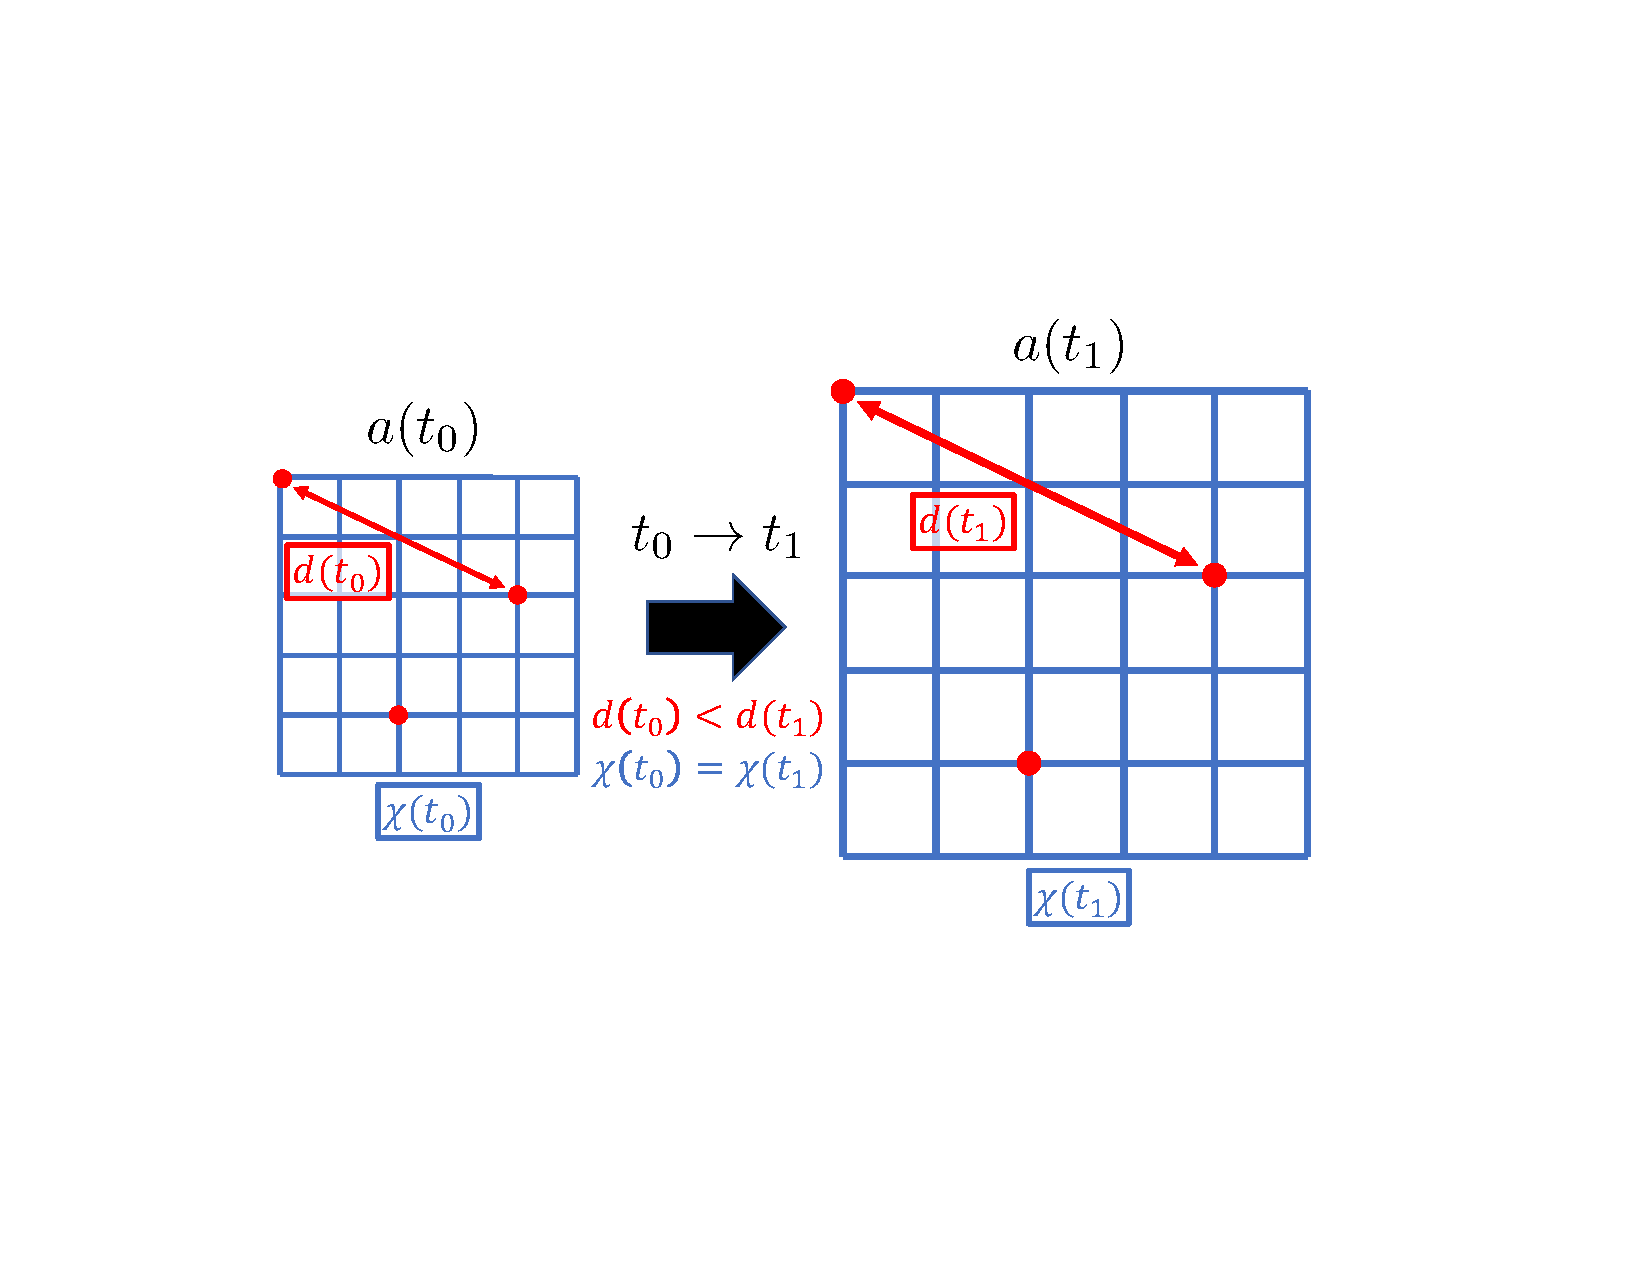
\includegraphics[width=0.9\linewidth, trim=3cm 5.5cm 3cm 5cm, clip]{ScientificMotivation/Figures/comoving_grid.pdf}
    \caption[A schematic of the comoving grid]{A schematic of the comoving grid. In the standard cosmological paradigm, the scale factor $a(t)$ grows with time, enlarging the distance between otherwise stationary objects, which are represented by red circles. However, in comoving coordinates, the distance between these objects remains constant.}
    \label{fig:comoving_grid}
\end{figure}

The solution Einstein's field equations given the FRW metric are
\begin{eqnarray}
    \left( \frac{\dot a}{a} \right)^{2} & = & \frac{8 \pi G}{3} \rho - \frac{k}{a^{2}} \\
    \frac{\ddot a}{a} & = & - \frac{4 \pi G}{3} \left( \rho + 3p \right) \, ,
    \label{eq:friedmann_equations}
\end{eqnarray}
where the overdots denote time derivatives, $\rho$ is energy density, and $p$ is isotropic pressure. These \textit{Friedman Equations} relate the universe's expansion history to that of its constituents and are the cornerstone of Big Bang cosmology. The expansion factor at present time is defined to be $a = 1$, and its time derivative is parameterized by the Hubble parameter
\begin{equation}
    H \equiv \frac{\dot a}{a} \, ,
    \label{eq:hubble_constant}
\end{equation}
which measures the rate at which space is expanding.

\begin{figure}
    \subfloat[\label{fig:hubble_diagram:a}]{
        \raisebox{1cm}{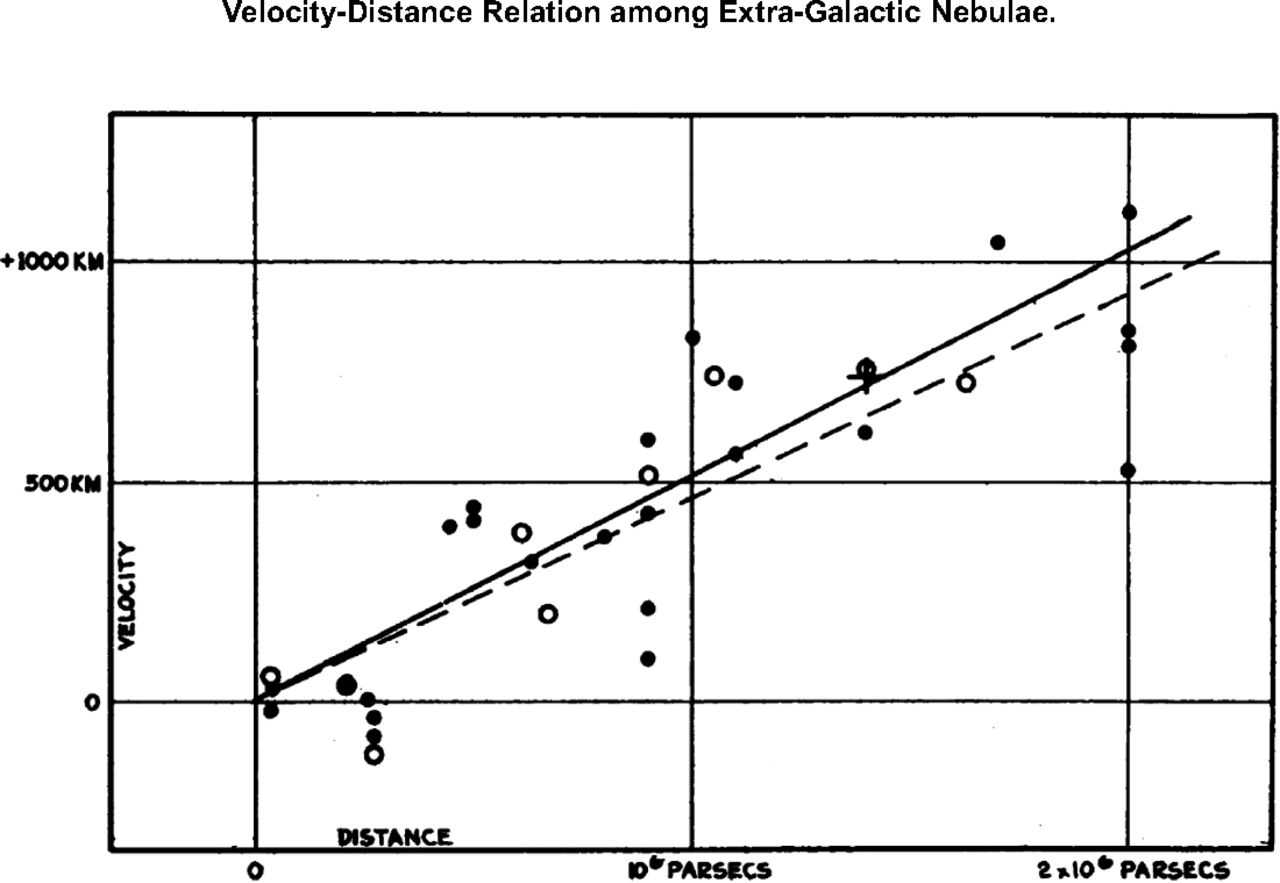
\includegraphics[width=0.48\linewidth]{ScientificMotivation/Figures/Hubble_redshiftRelation_1929.jpg}}
    }
    \subfloat[\label{fig:hubble_diagram:b}]{
        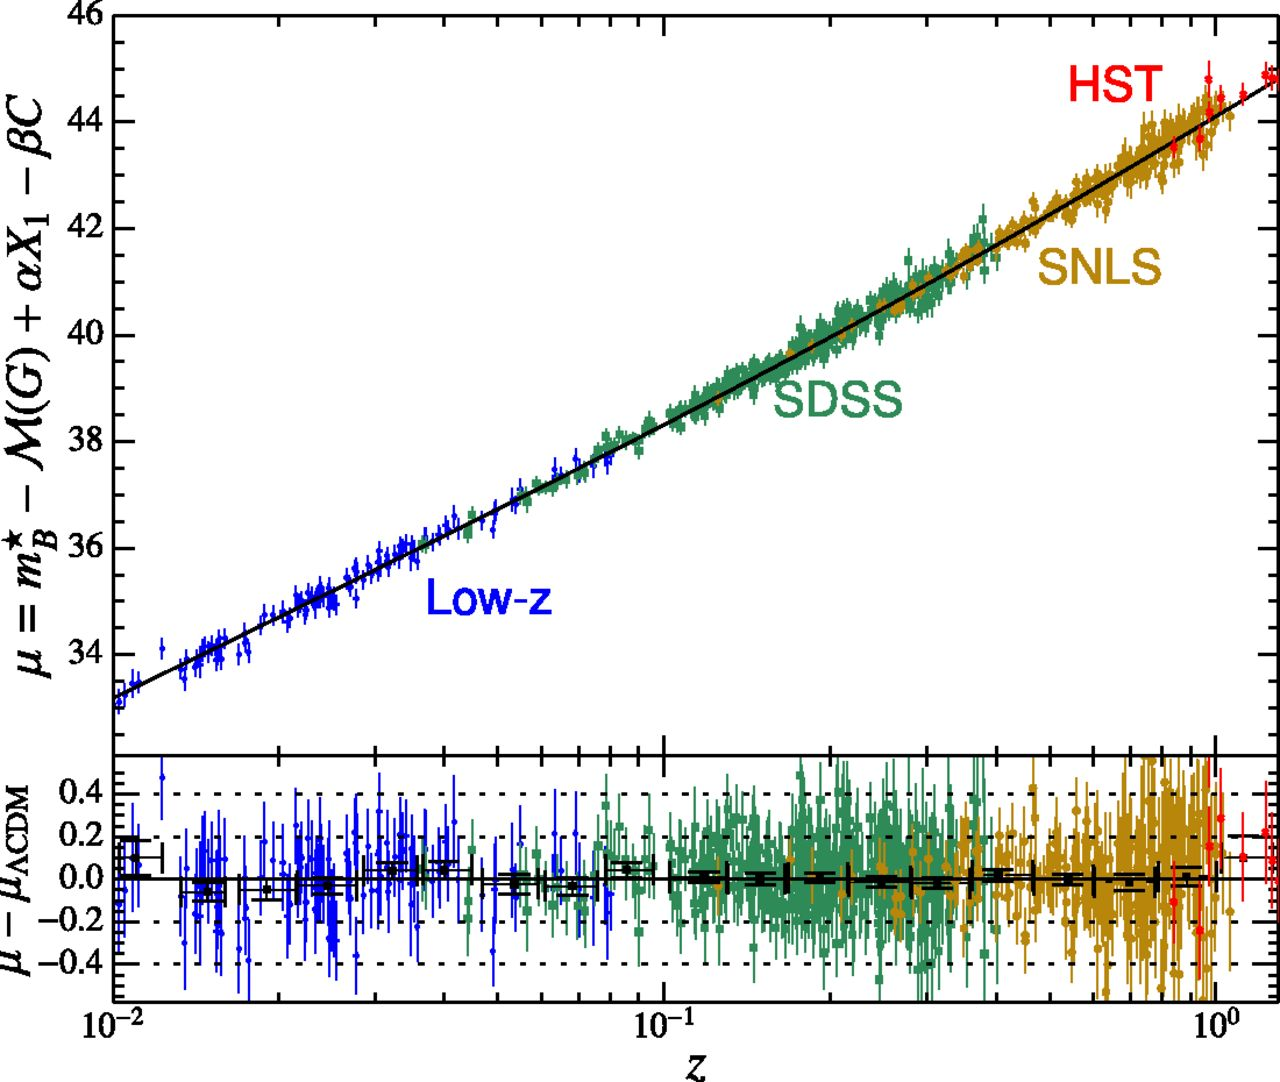
\includegraphics[width=0.48\linewidth]{ScientificMotivation/Figures/Bahcall_HubbleConstant_2015.jpg}
    }
    \caption[The original Hubble diagram and a modern version of it]{Two representations of the Redshift-velocity relationship, which is quantified by the Hubble constant. \ref{fig:hubble_diagram:a} shows Hubble's original diagram, published in 1929 \cite{hubble_relation_1929}. The filled circles and solid line show individual extra-galactic nebulae and distance-velocity relationship, respectively. The open circles and the dotted line show these nebulae grouped and fit. The clear trend demonstrates clearly that the universe is expanding. \ref{fig:hubble_diagram:b} shows a modern version of Hubble's plot, with collections of data from various experiments---Low-z, the Sloan Digital Sky Survey (SDSS), the Super Nova Legacy Survey, and the Hubble Space Telescope (HST)---which use supernovae to calibrate object distance \cite{bahcall_hubble_2015}.}
    \label{fig:hubble_diagram}
\end{figure}

The \textit{Hubble constant} $H_{0}$, or the current-time (a = 1) value of the Hubble parameter, was first measured by Edwin Hubble in 1929 using the redshift-distance relationship of extragalactic nebulae, as shown in Figure~\ref{fig:hubble_diagram:a}. Figure~\ref{fig:hubble_diagram:b} shows a a more modern measurement of $H_{0}$ from an assortment of telescopes and distant-ladder techniques, revealing a value of $H_{0} \approx 70$~km/s/MPc. While Hubble's measurement of turned out to be inaccurate, it was the first firm evidence for an expanding universe and birthed an era of precision cosmological measurements to characterize the dynamics of the universe on its largest scales.

We can conveniently rewrite the Friedmann equations in terms of the Hubble constant as
\begin{equation}
    H^{2} = H_{0}^{2} \left( \frac{\Omega_{r}}{a^{4}} + \frac{\Omega_{m}}{a^{3}} + \frac{\Omega_{k}}{a^{2}} + \Omega_{\Lambda} \right) \, ,
    \label{eq:friedmann_equation_densities}
\end{equation}
where $\Omega_{r}$, $\Omega_{m}$, $\Omega_{k}$, and $\Omega_{\Lambda}$ are the current-day densities of radiation, matter, curvature, and dark energy, respectively, with respect to the critical density
\begin{equation}
    \rho_{\mathrm{c}} = \frac{3}{8 \pi G} H_{0}^{2}\, .
    \label{eq:critical_density}
\end{equation}
The ratio of the actual density today to the critical density is given as $\Omega \equiv \rho_{0} / \rho_{\mathrm{c}}$ such that 
\begin{equation}
    \Omega = 1 + \frac{k}{H_{0}} \, ,
    \label{eq:total_density}
\end{equation}
The matter density $\Omega_{\mathrm{m}}$ includes that of dark matter, and the radiation density $\Omega_{\mathrm{r}}$ includes that of relativistic species. The best current estimates of the universe's constituents---most of which come from the Planck satellite mission---are shown in Table~\ref{tab:cosmological_parameters}. 

\begin{table}[]
    \centering
    \begin{tabular}{c|c}
         Parameter & Value \\
         \hline
         \hline
         $H_{0}$ & $67.66 \pm 0.42$ \\
         \hline
         $\Omega_{\mathrm{b}} h^{2}$ & $0.02242 \pm 0.00014$ \\
         \hline
         $\Omega_{\mathrm{c}} h^{2}$ & $0.14240 \pm 0.00087$ \\
         \hline
         $\Omega_{\mathrm{\Lambda}}$ & $0.6889 \pm 0.0056$ \\
         \hline
    \end{tabular}
    \caption{Cosmological parameters from Table~2 in the Planck 2018 publication. The error bars represent 68\% confidence limits, $\Omega_{\mathrm{k}} = 0$, as is true in a flat universe.}
    \label{tab:cosmological_parameters}
\end{table}

%%%%%%%%%%%%%%%%%%%%%%%%%%%%%%%%
%%%%%%%%%%%%%%%%%%%%%%%%%%%%%%%%
%%%%%%%%%%%%%%%%%%%%%%%%%%%%%%%%

\section{Cosmic microwave background}
\label{sec:cmb}

One of the most prominent predictions of the Big Bang model is the existence of a remnant background radiation. Because the universe is formed by the adiabatic expansion of space, at very early times, energy densities are very high, and therefore the universe's constituents---photons, electrons, positrons, protons, neutrons, and neutrinos---are in thermal equilibrium, forming what is often called the \textit{primordial plasma}. As the universe expands, its energy density dilutes (except for that of the cosmological constant) as in Equation~\ref{eq:friedmann_equation_densities}, and as the ``soup'' of particles cools, particles begin to decouple from the primordial plasma, or \textit{freeze out}. This process is called \textit{Big Bang Nucleosynthesis}, and it determines much of what we know about cosmic particle abundances today.

The ground-state binding energy of Hydrogen is 13.6~eV, and at temperatures substantially larger than this, ionizing radiation keeps Hydrogen atoms from forming. When in this state, the radiation and baryons compose a plasma, often called the \textit{baryon-photon fluid}, that is in thermal equilibrium. However, as the universe expands, the radiation energy dilutes, and the universe's temperature falls. At $T \sim 3500$~K, protons and electrons begin to combine to form neutral hydrogen, which in turn reduces the coupling between the photons and the baryonic matter. At $T < 3200$~K, enough neutral hydrogen has formed such that the radiation and baryonic matter are effectively decoupled, and the universe transitions into a transparent state, in which photons are allowed to stream freely. This event of Hydrogen formation is called \textit{recombination}, and the remnant radiation is called the \textit{cosmic microwave background} (CMB).

After recombination, the CMB energy density continues to dilute as $\Omega_{\mathrm{r}} / a^{4}(t)$, and its wavelength redshifts as
\begin{equation}
    \lambda(z) = \frac{\lambda_{0}}{(1 + z)} \, ,
    \label{eq:redshift}
\end{equation}
where $\lambda_{0}$ is the wavelength today ($z$ = 0) and the redshift $z$ is related to the scale factor as
\begin{equation}
    a = \frac{1}{1 + z}\, .
    \label{eq:redshift_to_scale_factor}
\end{equation}
Therefore, given that the CMB is expected to have decoupled at $T \sim 3500$~K and a redshift of $z \sim 1100$, we expect to observe a $T_{\mathrm{CMB}} \sim 2.7$~K background radiation today.

The CMB was discovered by Arno Penzias and Robert Wilson in 1964---only 55 years ago---by accident when trying to remove a persistent noise source their large horn antenna. The source was measured to be uniform across the sky with a temperature of 3.5~K. Many years later, the spectrum of the background radiation was measured by the Far Infrared Absolute Spectrometer (FIRAS) on the Cosmic Background Explorer (COBE) satellite. The measurement, shown in Figure~\ref{fig:cmb_spectrum} was performed using a carefully calibrated Fourier Transform Spectrometer (FTS) and is beautifully described by a blackbody
\begin{equation}
    B_{\nu}(T) = \varepsilon \frac{2 \nu^{2}}{c^{2}} \frac{h \nu}{e^{h \nu / (k_{\mathrm{B}} T)} - 1} \, , 
\end{equation}
with emissivity $\varepsilon = 1$ and temperature $T_{\mathrm{CMB}} = 2.73$~K. The current best estimate of the CMB temperature is
\begin{equation}
    T_{\mathrm{CMB}} = 2.7255 \pm 0.0006 \, ,
    \label{eq:cmb_temperature}
\end{equation}
which recalibrates the FIRAS data using data from WMAP, a CMB satellite that measured CMB anisotropies in the 1990s and early 2000s.

\begin{figure}
    \centering
    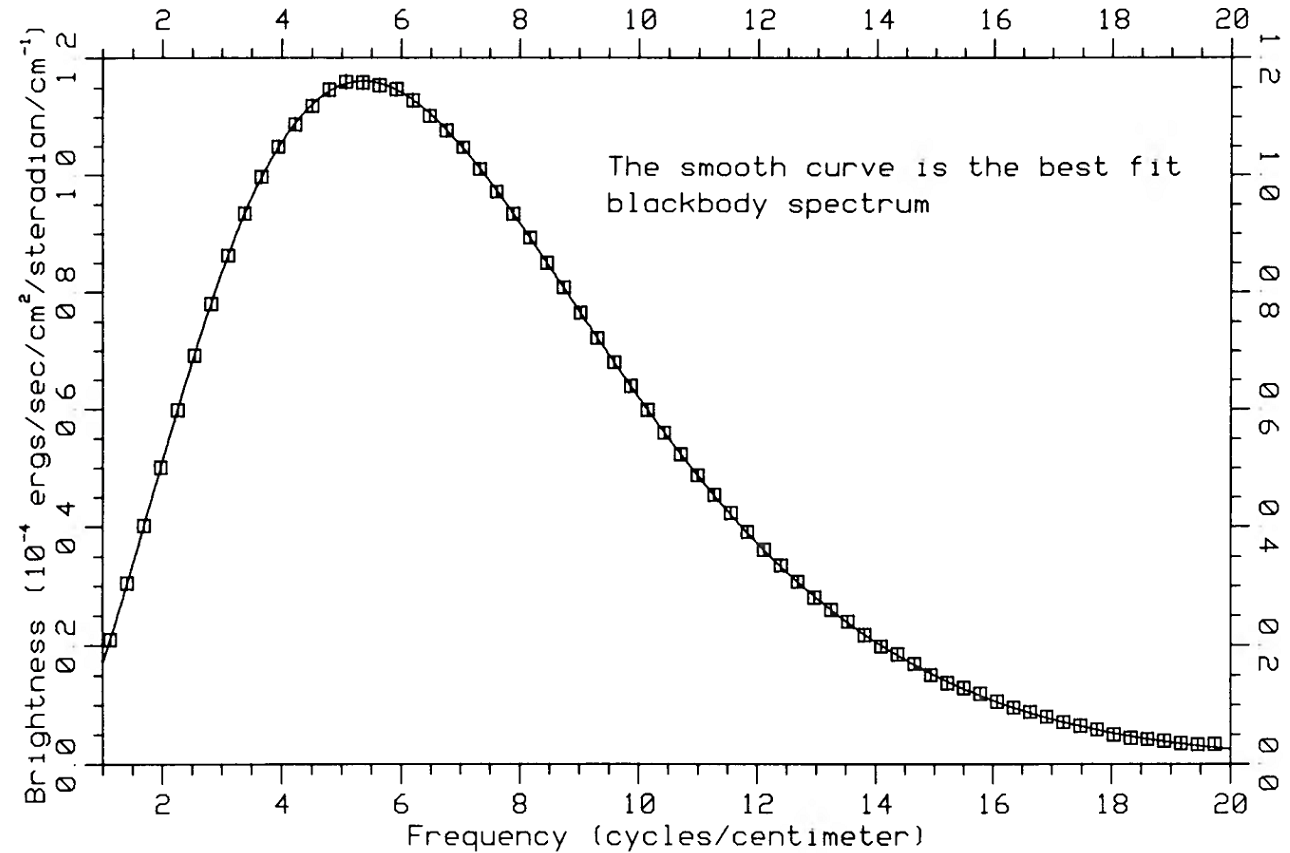
\includegraphics[width=0.7\linewidth]{ScientificMotivation/Figures/FIRAS_CMB_Spectrum_1990.png}
    \caption[FIRAS CMB spectrum (1990)]{Preliminary spectrum of the CMB measured by the FIRAS instrument on the COBE satellite, published in 1990 \cite{mather_preliminary_1990}. The box widths denote the frequency bins for each data point and heights denote a preliminarily stated error bar of 1\%. The error bar of the final spectrum, published in 1994, was orders of magnitude smaller \cite{fixsen_cosmic_1996}.}
    \label{fig:cmb_spectrum}
\end{figure}

In addition to FIRAS, the COBE satellite carried the Differential Microwave Radiometer, which made the first measurement of the CMB isotropy. The spatially mapped intensity fluctuations of the CMB were measured to be one part in ten thousand, demonstrating the extraordinary uniformity of the CMB across the sky. These intensity fluctuations offer a snapshot of the universe $\sim$~370,000 years after the Big Bang, and its hot and cold spots correspond to dark matter over- and under-densities in the primordial plasma. As we will discuss in Section~\ref{sec:anisotropies}, the CMB anisotropies are the seeds of structure formation on which our universe is built.

%%%%%%%%%%%%%%%%%%%%%%%%%%%%%%%%
%%%%%%%%%%%%%%%%%%%%%%%%%%%%%%%%
%%%%%%%%%%%%%%%%%%%%%%%%%%%%%%%%

\section{Inflation}
\label{sec:inflation}

Despite its success, the standard cosmological model fails to explain several outstanding mysteries. Some of these mysteries are at the interface of cosmology and particle physics,  such as $\Lambda$CDM's inability to describe the particle nature of dark matter and dark energy, its inability to describe the matter-antimatter asymmetry, and its predicted baryon abundance that is larger than that directly observed. However, some of the standard cosmological inconsistencies are ``internal,'' in that the assumptions of the model directly contradict the measurements on which it is built. The most prominent of these are...

\begin{itemize}
    \item Horizon problem: the universe appears to have equilibrated across super-horizon length scales, or larger distances than could have ever been in causal contact.
    \item Flatness problem: The universe observed today is very flat, and because any deviation from flatness grows with time, the universe must have begun with a flatness of one part in $\sim$~$10^{14}$, posing a fine-tuning issue.
    \item Magnetic monopole problem: magnetic monopoles are predicted by many grand unified theories, and yet we do not observe any.
    \item Initial conditions: $\Lambda$CDM shows that density perturbations in the early universe evolved into the large-scale structure that we see today. However it does not describe where these initial perturbations come from.
\end{itemize}

There have been several proposed extensions proposed to the Standard Model, but the most popular is \textit{inflation}. The theory of inflation states the universe went through a brief period of exponentially rapid expansion before the Standard Cosmological evolution began.

\begin{figure}[!t]
    \centering
    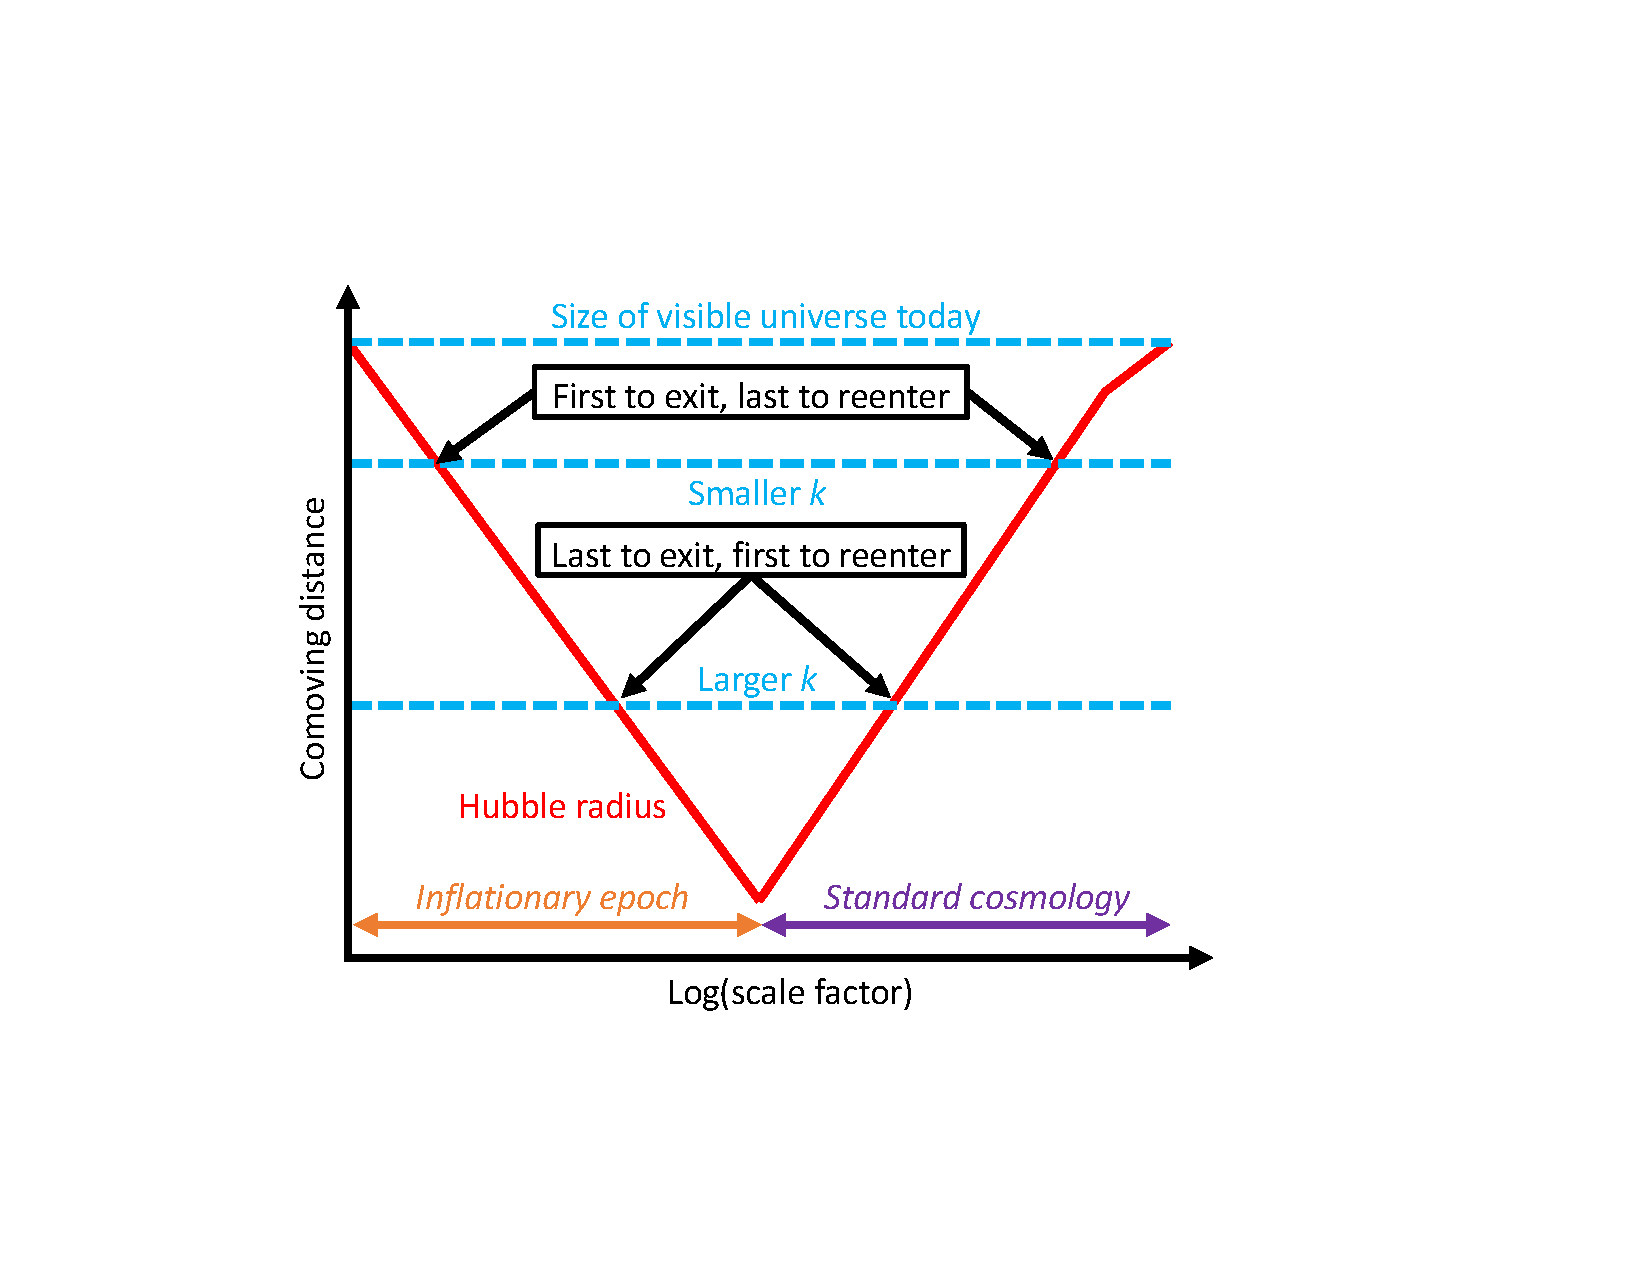
\includegraphics[width=0.6\linewidth, trim=5cm 4cm 7cm 4cm, clip]{ScientificMotivation/Figures/mode_exit_enter.pdf}
    \caption[A figure of mode exit and reentry in in the inflationary paradigm]{A qualitative representation of the relationship between the Hubble Radius---or equivalently the causal horizon---in units of comoving distance vs the scale factor during both the inflationary and standard cosmological epochs. During inflation, the Hubble radius shrinks, freezing length scales that were once in causal contact outside the causal horizon. During the standard cosmological evolution, the Hubble radius grows, and these scales reenter the horizon, allowing them to evolve. The horizontal lines show that small-scale fluctuations exit/enter the horizon first while large-scale fluctuations exit/enter the horizon last. The last scattering surface (LSS) is shown by a blue dotted line, and the kink in the Hubble radius at late times represents the transition from a radiation-dominated universe to a matter-dominated one.}
    \label{fig:mode_entry}
\end{figure}

Figure~\ref{fig:mode_entry} shows a schematic of how the inflationary epoch impacts both spacetime and causal distances. During inflationary expansion, all energy other than that of the inflation field---often called the ``inflaton''---is diluted away, enabling spacetime to expand exponentially.  This exponential expansion is not so different from the accelerating expansion that we witness today, which arises from the dominance of dark energy. Because this exponential expansion enables space to expand faster than the speed of light, the Hubble radius $R_{\mathrm{H}} = 1 / H$, or the length scale that could have at any time been in causal contact, shrinks in comoving coordinates. Note that the $1 / H_{0}$ roughly corresponds to the size of the observable universe today.

The dynamics of the inflationary epoch is governed by the \textit{inflaton}. If we assume that the inflaton is a scalar field $\phi$, as is often the case in the simplest inflationary theories, the Einstein field equations become
\begin{eqnarray}
    & & \ddot{\phi} + 3 H \dot{\phi} + V'[\phi] = 0 \\ 
    & & H^{2} = \frac{\rho_{\phi}}{24 \pi G} \\
    & &\rho_{\phi} = \frac{1}{2} \dot{\phi}^{2} + V[\phi] \, ,
    \label{eq:inflaton}
\end{eqnarray}
where $\phi$ is the inflaton field, $V[\phi]$ is the inflationary potential, and $\rho_{\phi}$ is the inflaton energy density. The first equation, which governs the inflaton's evolution, is nothing more than that of a harmonic oscillator, damped by the Hubble parameter. 

In order to solve the flatness, and horizon problems, the inflaton must follow several \textit{slow-roll} conditions, the dynamics of which are similar to the familiar behavior of a particle in a potential. The slow roll conditions are often given in terms of the \textit{slow-roll parameters}
\begin{equation}
    \epsilon \equiv \frac{m_{\mathrm{pl}}^{2}}{2} \left( \frac{V'[\phi]}{V[\phi]} \right)^{2} \ll 1 \; \; ; \; \; \eta \equiv m_{\mathrm{pl}}^{2} \left| \frac{V''[\phi]}{V[\phi]} \right|, ,
    \label{eq:slow_roll_parameters}
\end{equation}
where $m_{\mathrm{pl}} \equiv \sqrt{\hbar c / G} \sim 10^{19}$~GeV is the Planck mass. These slow roll parameters in turn determine the number of e-folds---or the logarithmic duration---over which inflation occurred
\begin{equation}
    N_{e} = \frac{1}{m_{\mathrm{pl}}} \left| \int_{\phi_{\mathrm{end}}}^{\mathrm{\phi}} \frac{\dd \phi}{\sqrt{2 \epsilon(\phi)}} \right| \simeq 60 - \log{\frac{10^{16} \, \mathrm{GeV}}{V^{1/4}}} \, ,
    \label{eq:efolds}
\end{equation}
where $V$ is the \textit{energy scale of inflation}. As suggested by the approximation in Equation~\ref{eq:efolds}, the number of e-folds needed to resolve the inconsistencies of the standard model is $\sim$~60, which determines, to within an order of magnitude or two, the inflationary energy scale.

\begin{figure}[!t]
    \centering
    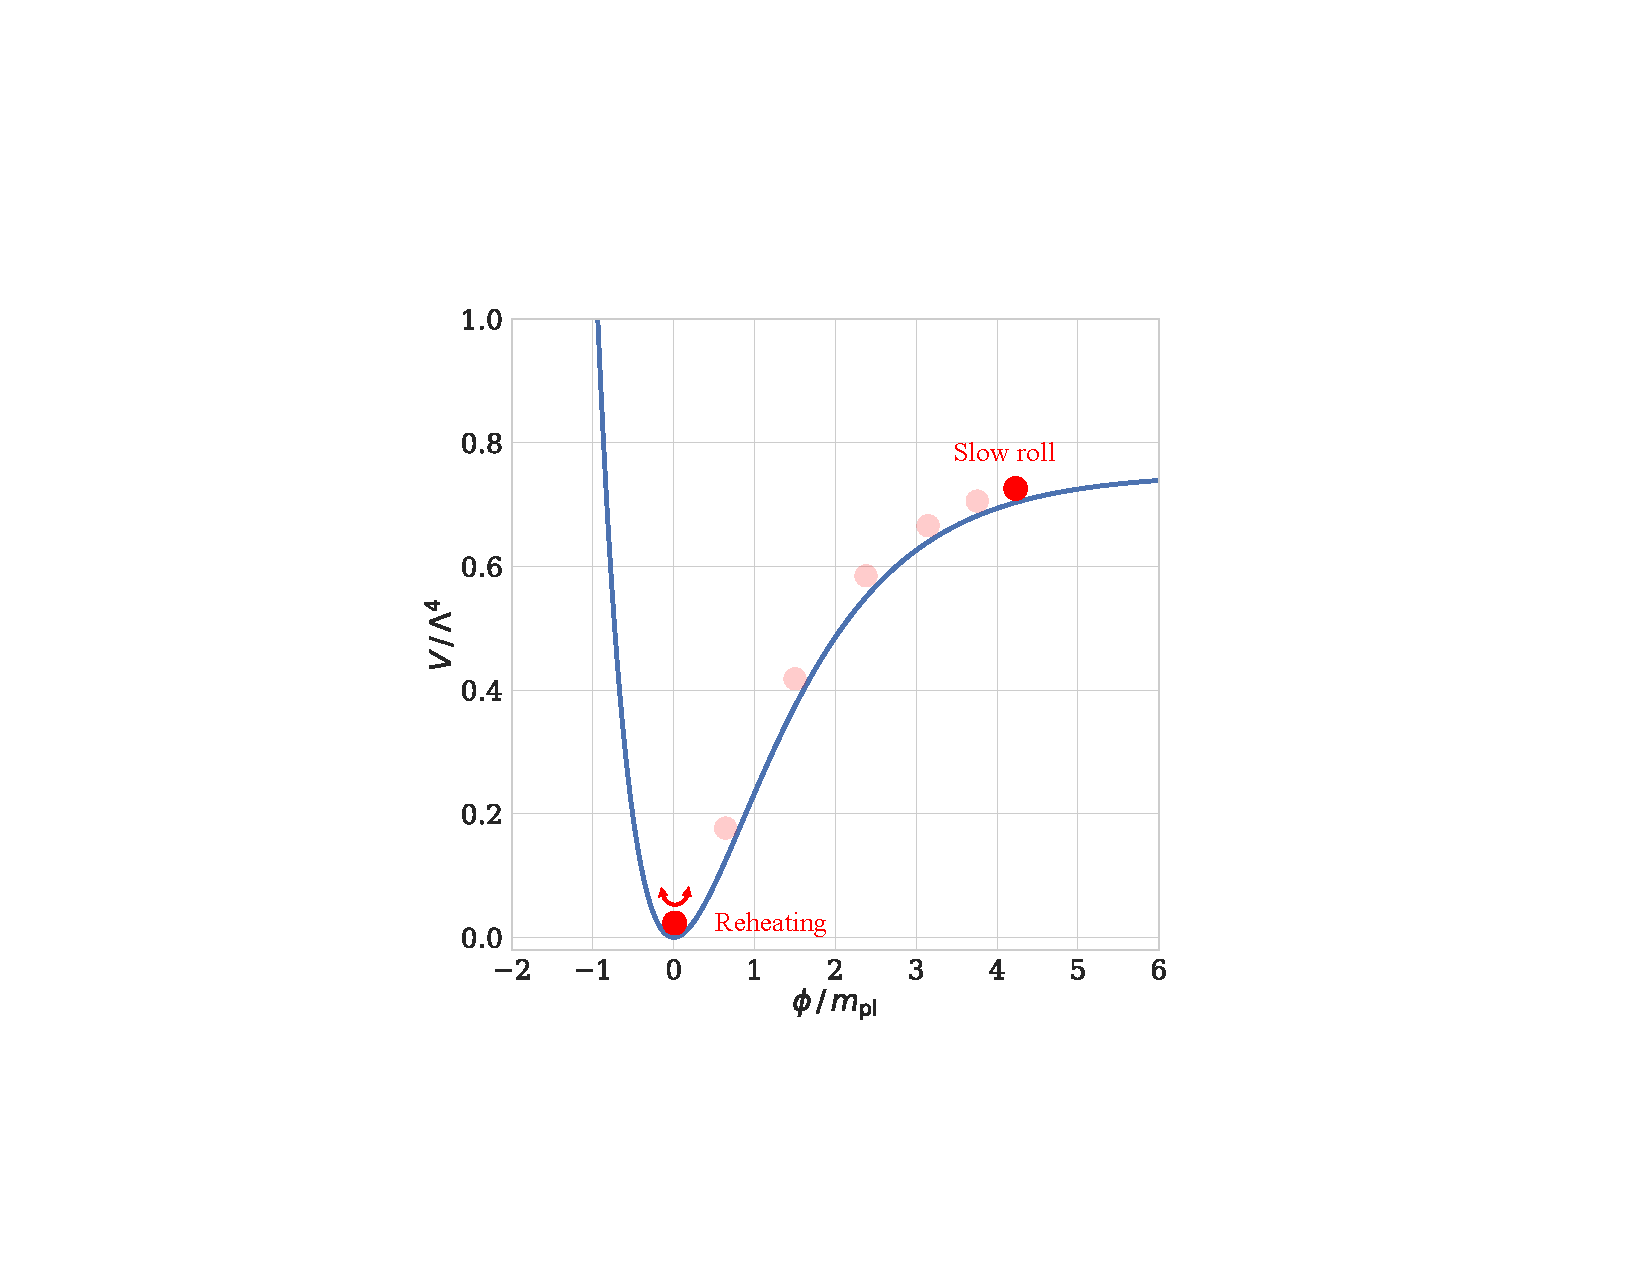
\includegraphics[width=0.7\linewidth, trim=6cm 4cm 6cm 5cm, clip=True]{ScientificMotivation/Figures/inflation_potential.pdf}
    \caption[The $R^{2}$ inflationary potential, which serves as an instructive example of slow-roll inflation.]{}
    \label{fig:inflation_potential}
\end{figure}

As an instructive example, let us consider the potential for Alexei Starobinsky's $R^{2}$ Inflationary Model. This particular model is classified as being \textit{small field} and is derived from a proposed modification to the Einstein-Hilbert action
\begin{equation}
    S = \frac{1}{2 \kappa} \int R \sqrt{| g |} \dd^{4}x \, \rightarrow S_{R^{2}} = \frac{1}{2 \kappa} \int \left(R + \frac{R^{2}}{6 M^{2}} \right) \sqrt{| g |} \dd^{4}x \, ,
    \label{eq:R2_action}
\end{equation}
where $\kappa \equiv 8 \pi G / c^{4}$ is so-called Einstein gravitational constant, $R$ is the Ricci curvature, and $M$ is the model parameter. The potential is found from solving the $R^{2}$ action
\begin{equation}
    V_{R^{2}}[\phi] = \Lambda^{4} \left[ 1 - \exp \left( - \sqrt{2 / 3} \phi / m_{\mathrm{pl}} \right) \right]^{2} \, ,
    \label{eq:starobinsky_potential}
\end{equation}
where $\Lambda$ is the cosmological constant.
The potential is shown in Figure~\ref{fig:inflation_potential} along with a cartoon of the how the inflaton evolves according to Equation~\ref{eq:inflaton}. At $t = 0$, the inflaton is said to be in a ``false vacuum,'' or equivalently an unstable equilibrium. The false vacuum can be constructed in many ways, such as a saddle point, a local minimum in $V[\phi]$, or a flat region, such as for the $R^{2}$ model. At the beginning of inflation, the inflaton \textit{rolls} slowly such that the kinetic term $3 H \dot{\phi} \approx 0$, enabling exponential expansion. However, as the kinetic term grows, both due to an exponentially growing Hubble parameter and due to increasing inflaton evolution, and as the potential term falls near zero, the inflaton decays in a process called \textit{reheating} into the constituents of the standard model. At this point, inflation ends, and the standard cosmological evolution begins.

There are several important outcomes of the inflationary epoch that are compelling within the framework of modern cosmology. First, the the inflationary expansion of spacetime---or equivalently the inflationary contraction of the Hubble radius---allowed the entire observable universe to thermalize prior to $\Lambda$CDM evolution, which solves the horizon problem. Second, the exponential expansion of space would've vastly diluted any spacetime curvatuve that was present at the Big Bang, giving rise to the flat universe we observe today. Third, in a similar manner, the rapid expansion of space would've vastly reduced the density of magnetic monopoles predicted at grand-unified energy scales to a scarcity consistent with their apparent nonexistence today. And finally, quantum fluctuations of the inflation field would have coupled to the metric, in turn seeding the Gaussian-random density variations that we observe in the CMB, hence solving the initial conditions problem.

Despite inflation's elegance and wide popularity, it is not the only proposed extension to the standard model that solves the flatness, horizon, monopole, and intial conditions problems. A prominent competitor is the Ekpyrotic model, which states that the universe is trapped in a never-ending cycle of expanding and collapsing. While Ekpyrosis also solves the horizon, flatness, magnetic monopole, and initial conditions problems, there is one signature that if observed would be a smoking-gun proof that the inflationary paradigm is indeed true: primordial gravitational waves.

Perturbations to the metric are typically classified into three categories: scalar, vector, and tensor. The scalar perturbations arise from density fluctuations, which are sourced by gravity and therefore evolve with underlying dark matter overdensities. Vector perturbations arise from the vortical motions of matter, which are not enhanced by gravity and therefore rapidly die out as the universe expands. Tensor perturbations arise from transverse-traceless perturbations to the metric that propagate by stretching and compressing spacetime, and therefore these tensor perturbation are equivalent to \textit{gravitational waves}. While both inflatin and Ekpyrosis produce Gaussian-random scalar fluctuations, only inflation would have produced a background of primordial gravitational waves.

It is both convenient and powerful to discuss density fluctuations in terms of its power spectrum
\begin{equation}
    \left< \delta(\vec{k}) \delta(\vec{k}') \right> \sim \frac{\delta^{3}(\vec{k} - \vec{k}')}{k^{3}} P(\vec{k})
    \label{eq:density_power_spectrum}
\end{equation}
where the $\sim$ denotes the limit of no mode coupling---enforced by the three-dimensional Dirac delta function---and where $k = | \vec{k} |$. It's worth emphasizing that $k$ is a wavenumber, and therefore large $k$ corresponds to short lengthscales and vice versa. A given mode is able to evolve as long as its wavelength is shorter than the Hubble radius $R_{\mathrm{H}}$, or equivalently when $k \lesssim a H$. As shown in Figure~\ref{fig:mode_entry}, during inflation the Hubble radius rapidly decreases, \textit{freezing out} modes such that they can no longer evolve. In other words, the superluminal expansion of space separates points in space that before inflation were in causal contact. When $k < a H$, the mode can no longer evolve, and it is ``frozen'' until the Hubble radius expands enough for the mode to re-enter the horizon. 

While the Gaussian fluctuations of the inflaton field are thought to be scale independent, the modes exit the horizon from low $k$ to high $k$ as the inflation field $\phi$ rolls down the potential $V[\phi]$, as shown in Figure~\ref{fig:mode_entry}. Therefore, there is a slight tilt in the expected scalar spectrum
\begin{equation}
    P_{\zeta}(k) \equiv A_{\mathrm{s}} \left( \frac{k}{k_{*}} \right)^{n_{\mathrm{s}}(k) - 1} \sim \frac{H_{*}^{2}}{\epsilon_{*} m_{\mathrm{pl}}^{2}} \, ,
    \label{eq:scalar_spctrum}
\end{equation}
where $H_{*}$ and $\epsilon_{*}$ denote the values of the Hubble parameter and the first slow roll parameter, respectively, when the mode $k$ exited the horizon. The spectral tilt is parameterized by the \textit{scalar index}
\begin{equation}
    n_{\mathrm{s}}(k) \equiv 1 + \frac{\dd \log P_{\zeta}(k)}{\dd \log k}
    \, .
    \label{eq:scalar_index}
\end{equation}
In a similar manner, the power spectrum of the tensor perturbations follows the relation
\begin{equation}
    P_{\mathrm{t}}(k) \equiv A_{\mathrm{t}} \left( \frac{k}{k_{*}} \right)^{n_{\mathrm{t}}(k)} \sim \left( \frac{H_{*}}{m_{\mathrm{pl}}} \right)^{2} \, ,
    \label{eq:tensor_spectrum}
\end{equation}
and the tensor index is defined as
\begin{equation}
    n_{\mathrm{t}}(k) \equiv \frac{\dd \log P_{t}(k)}{\dd \log k} \, .
    \label{eq:tensor_index}
\end{equation}
Using these conventions, we expect $n_{\mathrm{s}}$ to be close to 1 and $n_{\mathrm{t}}$ to be close to 0, and we expect each to have a slightly negative slope with $k$. 

The amplitude of the tensor power spectrum is often quoted using the \textit{tensor-to-scalar ratio}
\begin{equation}
    r_{*} \equiv \frac{P_{\mathrm{t}}(k_{*})}{P_{\mathrm{\zeta}}(k_{*})} = \frac{A_{\mathrm{s}}}{A_{\mathrm{t}}} \sim 16 \frac{V_{*}}{A_{\mathrm{s}} m_{\mathrm{P}}^{4}} \, ,
    \label{eq:tensor_to_scalar_ratio}
\end{equation}
where $k_{*}$ is a mode number often chosen by convention by convention to be $k_{*} = 0.05$~$\mathrm{MPc^{-1}}$ and where $V_{*}$ is the inflationay energy scale when mode $k_{*}$ exits the horizon. The tensor-to-scalar ratio can be written in terms of the energy scale of inflation as
\begin{equation}
    V_{*}^{1/4} = 10^{16} \, \mathrm{GeV} \, \left( \frac{r_{*}}{0.01} \right)^{1/4} \, .
    \label{eq:tensor_to_scalar_energy_scale}
\end{equation}
Because the the dependence of the inflationary potential on the tensor to scalar ratio is shallow, a detection of $r_{*}$ would provide a tight constrain $V_{*}$. However, if $V_{*}$ is much lower than the grand unified energy scale $10^{19}$~GeV, then $r_{*}$ may be undetectably small.

%%%%%%%%%%%%%%%%%%%%%%%%%%%%%%%%
%%%%%%%%%%%%%%%%%%%%%%%%%%%%%%%%
%%%%%%%%%%%%%%%%%%%%%%%%%%%%%%%%

\section{CMB anisotropies}
\label{sec:anisotropies}

As discussed in Section~\ref{sec:cmb}, CMB anisotropies trace the underlying dark matter density fluctuations at the time of recombination, and therefore studying their properties illuminates physics of the early universe. The latest full-sky measurement of CMB temperature and polarization anisotropies is from the Planck satellite, and their maps are shown in Figure~\ref{fig:cmb_maps}. 

\begin{figure}[!ht]
    \centering
    \subfloat[\label{fig:cmb_maps:a}]{
        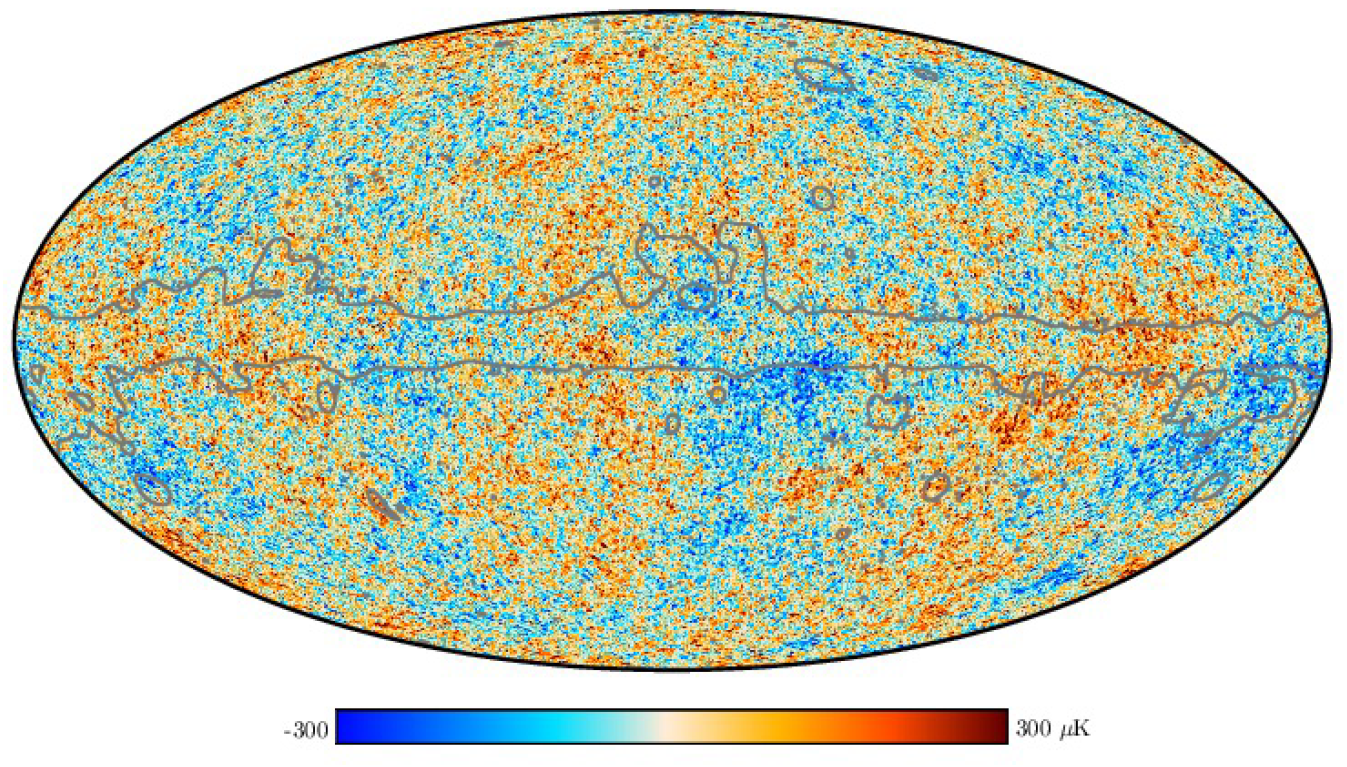
\includegraphics[width=0.7\linewidth]{ScientificMotivation/Figures/Planck_CMB_temperature_2019.png}
    }
    \hfill
    \subfloat[\label{fig:cmb_maps:b}]{
        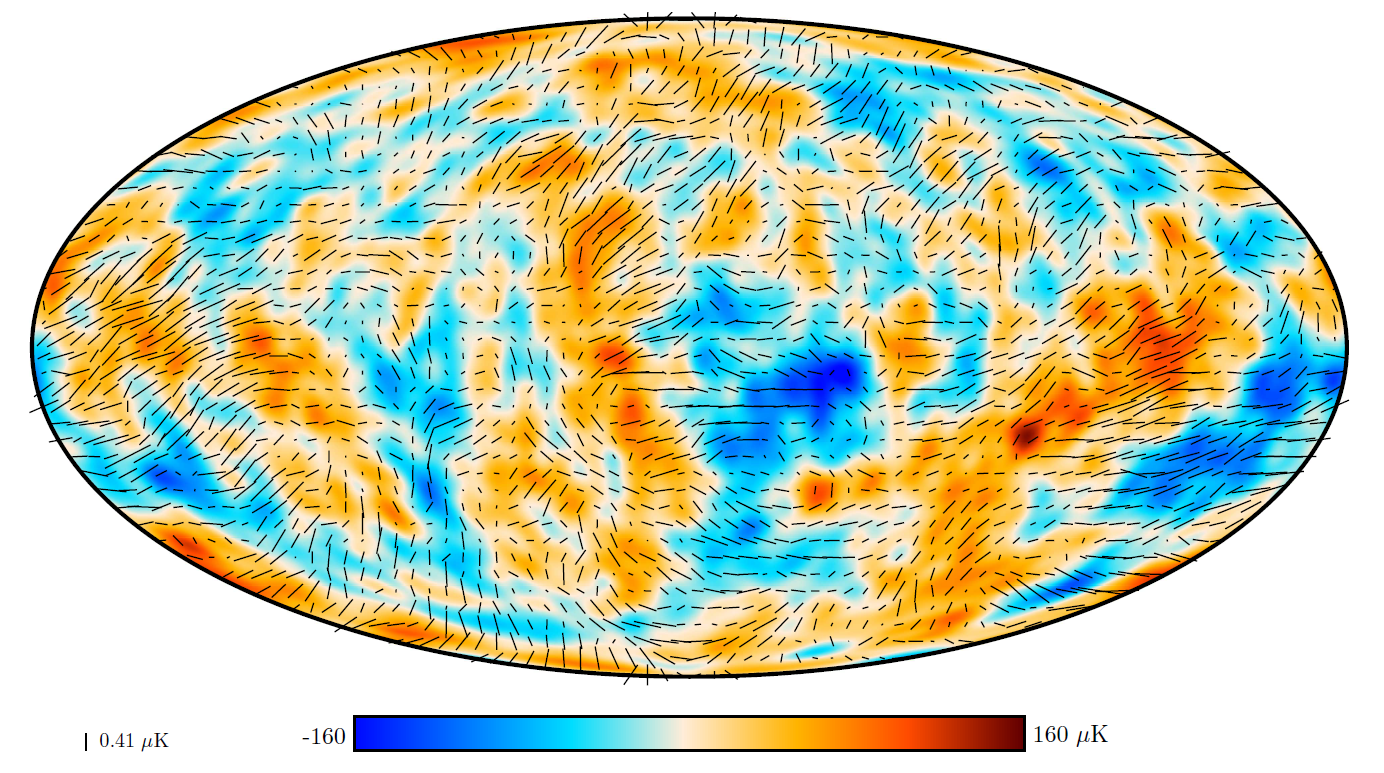
\includegraphics[width=0.7\linewidth]{ScientificMotivation/Figures/Planck_CMB_polarization_2019.png}
    }
    \caption[Planck full-sky CMB temperature and polarization maps (2018)]{Full-sky map of the CMB as presented in the Planck satellite 2018 data release \cite{planck_collaboration_planck_2019}. \ref{fig:cmb_maps:a} shows the temperature anisotropies, with the dominant foreground regions, which are centered around the galactic plane, masked out. \ref{fig:cmb_maps:b} shows the polarization anisotropies smoothed to an angular resolution of 5 degrees for visual clarity.}
    \label{fig:cmb_maps}
\end{figure}

Because the CMB pervades all space and therefore fills the full sky, we can conveniently decompose its temperature fluctuations into spherical harmonics
\begin{equation}
    \Delta T(\hat{n}) = \sum_{\ell = 0}^{\infty} \sum_{m = \ell}^{\ell} a_{\ell m} Y_{\ell m}(\hat{n}) \, ,
    \label{eq:spherical_harmonics}
\end{equation}
where $\hat{n}$ denotes a location on the sky, $(\ell, m)$ are the mode numbers, and $a_{\ell m}$ are the mode amplitudes. As predicted by inflation, the anisotropies of the CMB are isotropic (except the dipole, which arises due to our local motion with respect to the cosmic rest frame) and largely\footnote{As we discuss in Section~\ref{sec:foregrounds}, secondary anisotropies give rise to small levels of non-Gaussianity.} Gaussian, allowing their statistics to be well-described by the temperature power spectrum
\begin{equation}
    \left< \Delta T(\hat{n}) \Delta T(\hat{n}') \right> = \frac{1}{4 \pi} \sum_{\ell = 0}^{\infty} (2 \ell + 1) \, C_{\ell} P_{\ell}(\hat{n} \cdot \hat{n}') \, ,
    \label{eq:temperature_power_spectrum}
\end{equation}
where $P_{\ell}(\cos \theta_{\mathrm{sky}})$ are Legendre Polynomials and the mode variances are defined to be
\begin{equation}
    \left< a_{\ell m} a^{*}_{\ell' m'} \right> = \delta_{\ell m} \delta_{\ell' m'} C_{\ell} \, .
    \label{eq:C_ell}
\end{equation}
$C_{\ell}$ is the variance of the distribution for all $-\ell < m < \ell$ and is a physical measure of the fluctuations for mode $\ell$. Because $\ell = 1$ corresponds to the dipole, the simple relationship 
\begin{equation}
    \theta_{\mathrm{sky}} \sim \frac{180^{\circ}}{\ell} \, ,
    \label{eq:ell_theta_relation}
\end{equation}
relates spherical harmonic mode number to angle on the sky.

For a given $\ell$, there are only $2 \ell + 1$ $m$'s, which means there is a limit to how well one can measure each mode's variance $C_{\ell}$. This limit is called \textit{cosmic variance} and is defined as
\begin{equation}
    \Delta C_{\ell}^{2} = \frac{2}{(2 \ell + 1) f_{\mathrm{sky}}} C_{\ell}^{2} \, ,
    \label{eq:cosmic_variance}
\end{equation}
where $f_{\mathrm{sky}}$ is the fraction of the sky which is measured. The reality of cosmic variance has two important implications for CMB anisotropy measurements. First, because $\Delta C_{\ell} \propto C_{\ell}$, one cannot measure the any given $a_{\ell m}$ distribution with infinite precision, no matter how big the signal is. Second, because larger angular scales have fewer $m$'s, their measurement is more likely to become \textit{cosmic-variance limited}, often motivating larger sky coverage $f_{\mathrm{sky}}$ when measuring low-$\ell$.

\begin{figure}[!t]
    \centering
    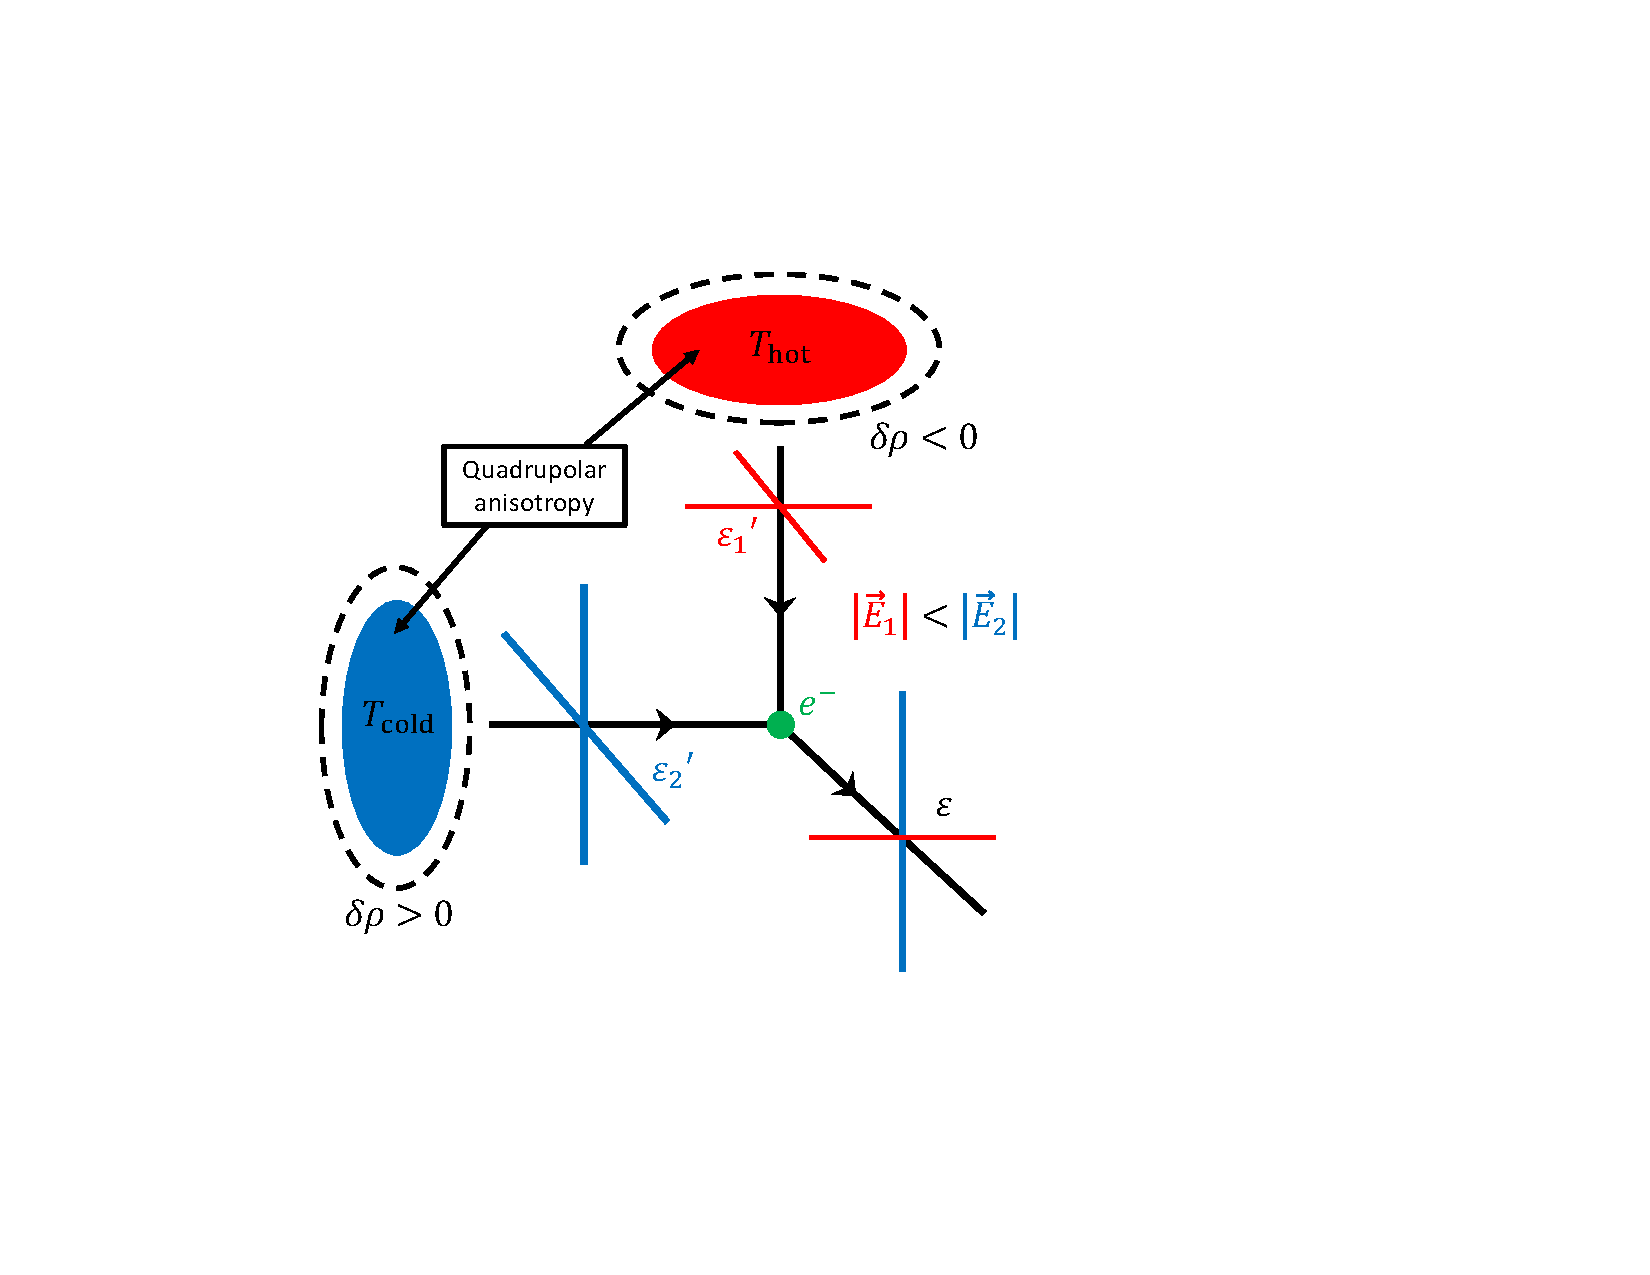
\includegraphics[width=0.5\linewidth, trim=5cm 5cm 10cm 4.5cm, clip]{ScientificMotivation/Figures/thomson_scattering.pdf}
    \caption[Thomson scattering of CMB quadrupolar anisotropies]{A schematic of how temperature anisotropies give rise to linear CMB polarization. Hot/cold spots correspond to gravitational over/underdensities and as photons climb/fall out of these potential wells, they lose/gain momentum $p = h \lambda$, which in turn causes their wavelength to shift down/up. Therefore, ``hot'' photons emerge from \textit{under}densities, while ``cold'' photons emerge from \textit{over}densities. At last scattering, these photons Thomson scatter from a ``taget'' electron $e^{-}$, and when the temperature anisotropy is quadrupolar, the scattered electric fields are not equal $|\vec{E}_{1}| < |\vec{E}_{2}|$, giving rise to a small degree of linear polarization.}
    \label{fig:thomson_scattering}
\end{figure}

In addition to temperature anisotropies, the CMB also contains polarization fluctuations. The CMB is polarized by Thomson scattering of quadrupolar anisotropies at the last scattering surface, as shown in Figure~\ref{fig:thomson_scattering}. The resulting polarization pattern on the sky is often conveniently decomposed into so-called \textit{E-modes} and \textit{B-modes}, which in the \textit{flat-sky approximation} are written as
\begin{eqnarray}
    E(\vec{\ell}) & = & Q(\vec{\ell}) \cos(2 \phi_{\vec{\ell}}) + U(\vec{\ell}) \sin(2 \phi_{\vec{\ell}}) \\
    B(\vec{\ell}) & = & U(\vec{\ell}) \cos(2 \phi_{\vec{\ell}}) - Q(\vec{\ell})\sin(2 \phi_{\vec{\ell}}) \, ,
    \label{eq:emodes_bmodes}
\end{eqnarray}
where $Q = \left< \left| E_{x} \right|^{2} \right> - \left< \left| E_{y} \right|^{2} \right>$ and $U = \left< \left| E_{a} \right|^{2} \right> - \left< \left| E_{b} \right|^{2} \right>$ are the linear-polarization Stokes parameters, $\vec{\ell}$ is the two-dimensional Fourier mode vector, which replaces the ($\ell$, $m$) indices, and $\phi_{\vec{\ell}}$ is the orientation of the mode vector. There are several important properties to notice about the E/B composition. First of all, they are spin-2 fields, meaning that they flip sign under a $\pi/2$ rotation. Secondly, unlike with $Q$ and $U$ explicitly, $E$ and $B$ are not defined with respect to a fixed coordinate system but are instead defined by their symmetry. Figure blah shows an illustration of each basis vector for comparison. E-modes have zero curl and a non-zero divergence, while B-modes have a zero divergence and a non-zero curl. In other words, E-modes have no handedness---or are mirror-symmetric---while B-modes do.

\begin{figure}[!t]
    \centering
    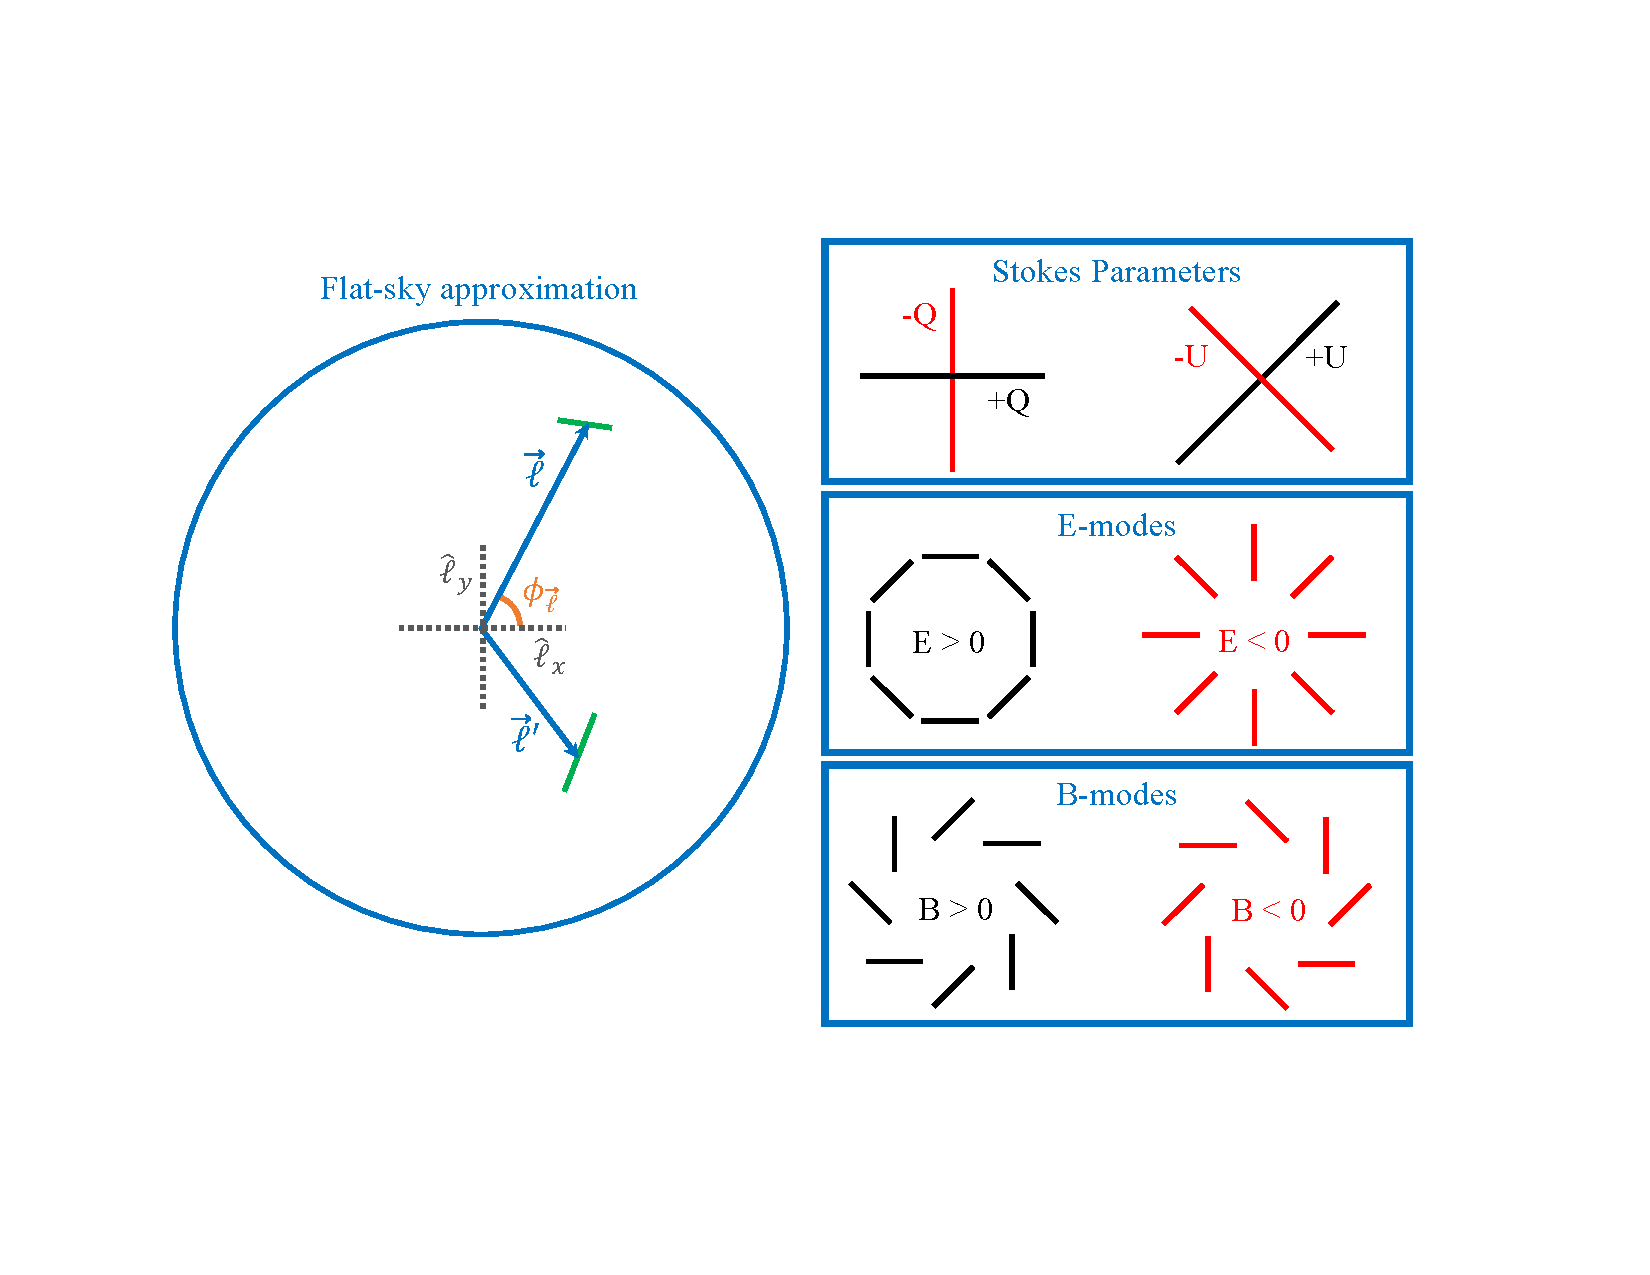
\includegraphics[width=0.8\linewidth, trim=2.5cm 4cm 3.5cm 4cm, clip]{ScientificMotivation/Figures/emodes_bmodes.pdf}
    \caption[Stokes parameters, E-modes, B-modes in the flat-sky approximation]{A schematic of the flat-sky approximation, which quantifies the spherical-harmonic modes using vector $\vec{\ell}$ instead of ($\ell$, $m$). In this scheme, the Stokes vectors Q/U are converted to E-modes and B-modes using Equations~\ref{eq:emodes_bmodes}. As shown in the right panel, E-modes are parity-even, while B-modes are parity-odd. The B-modes' handedness means that they cannot be generated by scalar fluctuations but only by tensor.}
    \label{fig:emodes_bmodes}
\end{figure}

The E-mode/B-mode decomposition is a powerful tool to study the CMB polarization. Because B-modes are only created by tensor perturbations, they are a \textit{null channel} via which primordial gravitational waves can be probed. In other words, a primordial B-mode detection would be a smoking-gun proof of inflation, and such a detection is not limited by cosmic variance (see Equation~\ref{eq:cosmic_variance}).\footnote{In reality, B-mode foregrounds obfuscate the gravitational wave signal, as we will discuss soon} In addition, though only generated by scalar perturbations, E-modes offer their own wealth of information about the univere and its evolution. Just as temperature anisotropies measure the density field of the primordial plasma, E-modes measure the \textit{velocity} field. Additionally, because the CMB is polarized at only the $\sim$~10\% level, the E-mode signal is substantially smaller than that of intensity, allowing for improved cosmic variance in the measurement of both the E-mode variance and the E-mode + temperature correlation. 

%%%%%%%%%%%%%%%%%%%%%%%%%%%%%%%%
%%%%%%%%%%%%%%%%%%%%%%%%%%%%%%%%
%%%%%%%%%%%%%%%%%%%%%%%%%%%%%%%%

\section{CMB power spectrum}
\label{sec:cmb_power_spectrum}

As discussed in Section~\ref{sec:anisotropies}, the fluctuations of the CMB temperature are Gaussian random and are therefore characterized by their variance. This variance depends mode number $\ell$ and is therefore well described by a power spectrum, which measures the amount of fluctuation per angular scale. In spherical-harmonic coordinates, the power spectrum is often written as
\begin{equation}
    D_{\ell}^{XX} = \frac{\ell (\ell + 1) C_{\ell}^{XX}}{2 \pi} \, ,
    \label{eq:D_ell}
\end{equation}
which is chosen for convention because it gives a temperature power spectrum that is roughly flat in $\ell$-space. Here, $XX = (TT, EE, BB, TE, TB, EB)$, noting that we can take various auto and cross spectra between temperature, E-mode, and B-mode fluctuations.

\begin{figure}[!t]
    \centering
    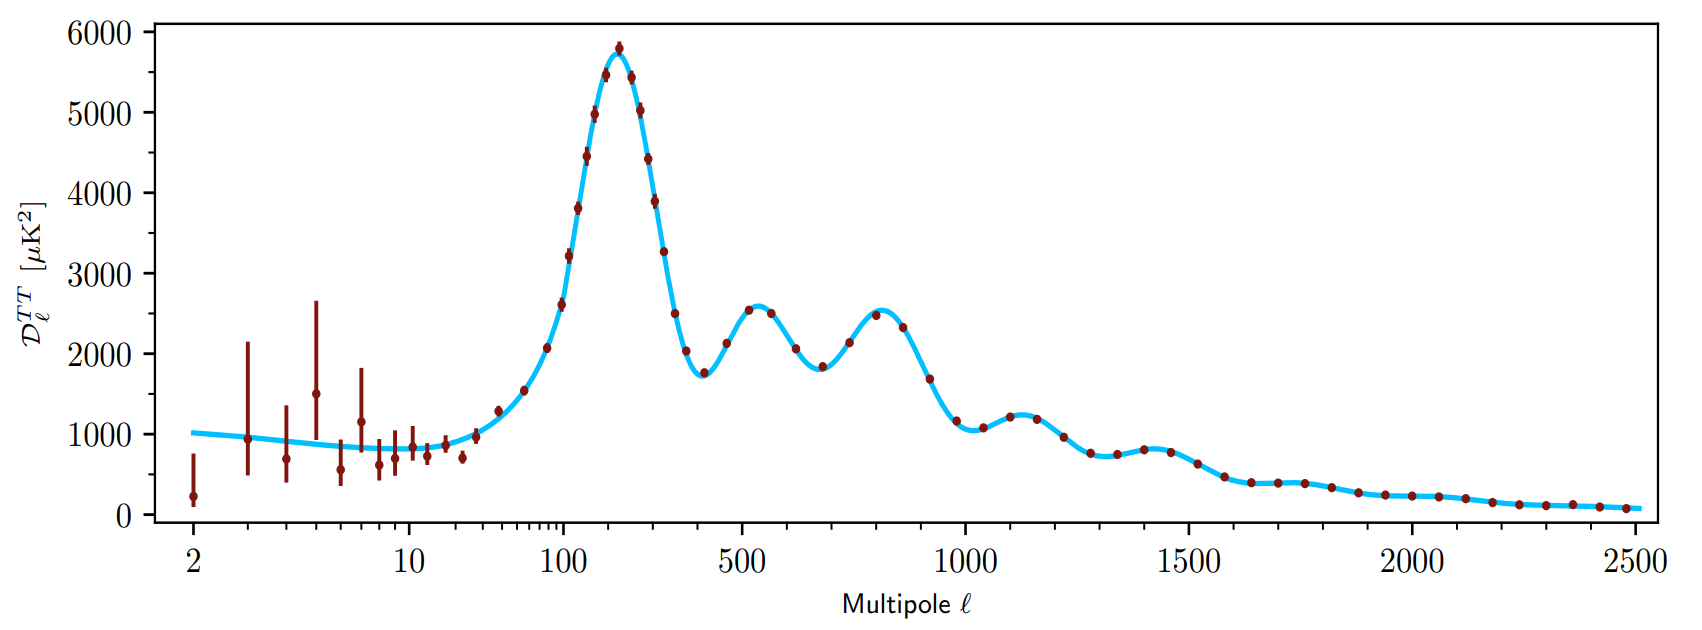
\includegraphics[width=\linewidth]{ScientificMotivation/Figures/Planck_CMB_temperatureSpectrum_2019.png}
    \caption[Planck TT power spectrum]{Autocorrelation power spectrum of the CMB temperature anisotropies as a function of angular scale, as determined using the Planck 2018 data release \cite{planck_collaboration_planck_2019}. The fit corresponds to a $\Lambda$CDM model with six free cosmological parameters: $\Omega_{\mathrm{m}}$, $\Omega_{\mathrm{b}}$, $\theta_{\mathrm{MC}}$, $\tau$, $n_{\mathrm{s}}$, $A_{\mathrm{s}}$. The exquisite precision over a wide range of angular scales is limited by cosmic variance, which fundamentally limits how well we can characterize the statistics of a single realization of the universe.}
    \label{fig:cmb_tt_spectrum}
\end{figure}

The temperature power spectrum, as measured by the Planck satellite, is shown in Figure~\ref{fig:cmb_tt_spectrum}, and it contains several important features that are worth noting. Mirroring the discussion in Section~\ref{sec:inflation}, we move from low-$\ell$ to high-$\ell$, which corresponds to the first/last modes to exit/enter the horizon in Figure~\ref{fig:mode_entry}. At $\ell \lesssim 100$, or on angular scales $\theta_{\mathrm{sky}} \lesssim 1^{\circ}$, the spectrum is nearly flat. These modes exist outside of the horizon at the time of last scattering and therefore have not evolved since they exited the horizon during the inflationary epoch. In principle, these low-$\ell$ modes could be used to measure $r$, as gravitational waves give rise to temperature fluctuations. However, $D_{\ell}^{TT}$ is dominated by gravitational redshifting at the surface of last scattering, also called the \textit{Sachs-Wolfe Effect}, and the measurement precision is limited by cosmic variance.

Moving to higher-$\ell$, there is a series of peaks which are generated by baryon acoustic oscillations (BAOs). Because these modes are of a shorter length scale, they enter the horizon before recombination and therefore evolved according to the physics of the primordial plasma. BAOs are acoustic waves that arise from compression due to gravitational dark matter overdensities and rarefaction due to photon pressure in the primordial fluid. The peaks in the spectrum correspond to the scales at which the oscillations are at maximum rarefaction (odd peaks) and maximum compression (even peaks). When the CMB decoupled, the baryonic matter was frozen into place, and their remnant was imprinted onto the CMB anisotropies. As the universe continues to evolve after recombination, the underlying dark matter densities cause the baryons to accumulate, leading to the formation of structure that we observe today. At $\ell \gtrsim 1000$ the BAO peaks are suppressed by \textit{Silk damping}, which arises when the length scale of the BAOs is shorter than the photon diffusion length. The impact of Silk damping is heightened by the finite duration of recombination, when the universe phase transitions from opaque to quite transparent. During the recombination epoch, the photon diffusion length increases rapidly, pushing the Silk damping tail to lower $\ell$ than if recombination had been instantaneous. 

As is evident in Figure~\ref{fig:cmb_spectrum}, the measurement of the temperature power spectrum is exquisite. The Planck satellite measured the full spectrum to nearly cosmic variance, and the data is described to very high prevision by $\Lambda$CDM. In addition, a plethora of experiments have independently verified the shown $TT$ spectrum across a range of $\ell$ from 2~$\sim$~5000 (above this scale, the measured temperature power spectrum becomes dominated by unresolved point sources, which are difficult to remove).

\begin{figure}[!t]
    \subfloat[\label{fig:cmb_ee_bb_spectrum:a}]{
        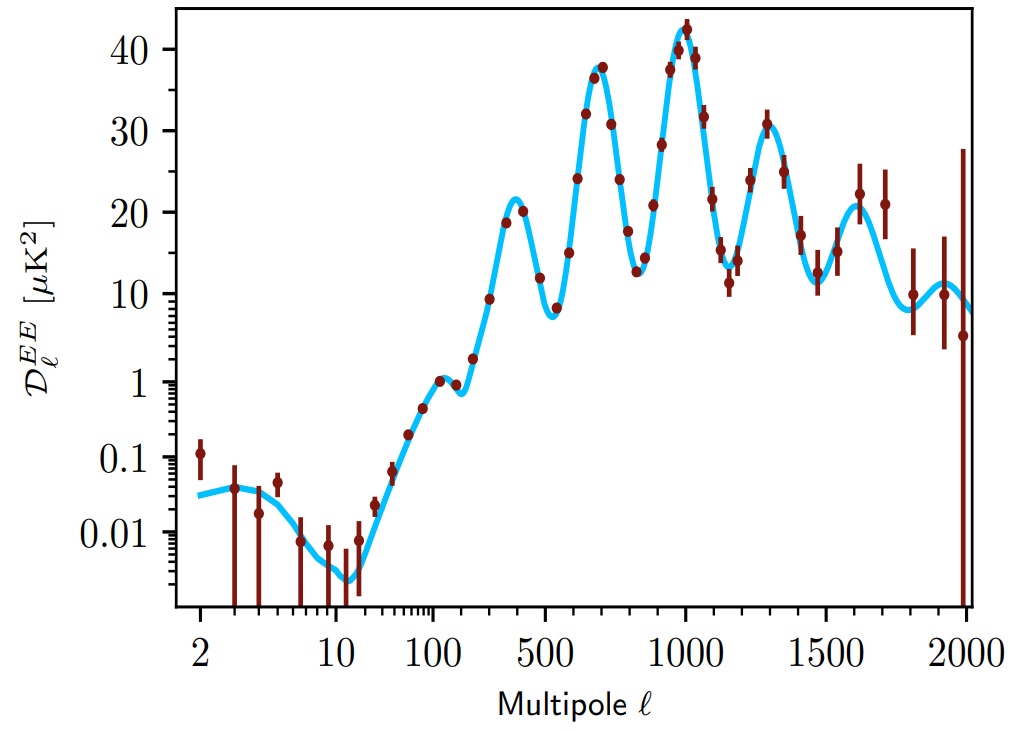
\includegraphics[width=0.6\linewidth, trim=0cm 0cm 0cm 0cm, clip]{ScientificMotivation/Figures/Planck_CMB_EEspectrum_2019.png}}
    \subfloat[\label{fig:cmb_ee_bb_spectrum:b}]{
        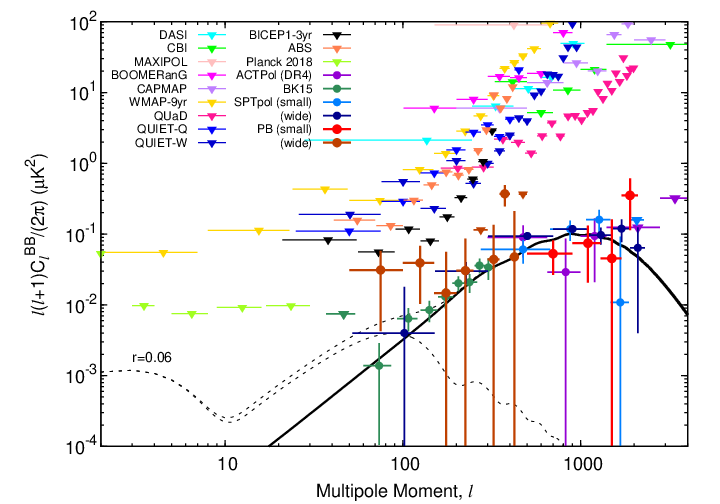
\includegraphics[width=0.6\linewidth, trim=0cm 0cm 0cm 0cm, clip]{ScientificMotivation/Figures/bb_yuji.png}}
    \caption{Power spectrum of the CMB E-mode anisotropies as measured by Planck (top panel) and B-mode anisotropies as measrued by several experiments. The $EE$ features are due to the velocity field of BAO and its fit uses the same cosmological parameters as that of Figure~\ref{fig:cmb_tt_spectrum}, while the B-mode spectrum arises due to gravitational lensing of the E-modes. The dotted lines represent the current 95\% upper limits on the primordial B-mode spectrum.}
    \label{fig:cmb_ee_bb_spectrum}
\end{figure}

CMB polarization measurements have just recently begun to come into focus. The EE spectrum, shown in the top panel of Figure~\ref{fig:cmb_ee_bb_spectrum}, is also generated by BAO but is the result of photon velocities, which create redshifts that when quadrupolar about the scattering electron, creating polarization via Thomson Scattering. Because quadrupolar BAO fluctuations are are less prominent than those of the monopole, the CMB's polarization fraction $\lesssim$~10\%, and the $EE$ spectrum is orders of magnitude below that of $TT$. Additionally, though both generated by BAO, the velocity-generated $EE$ peaks are out of phase with the density-generated $TT$ peaks. At $\ell \gtrsim 1500$, photon diffusion damps the $EE$ spectrum similarly to $TT$, but at low-$\ell$, the physics of temperature an polarization anisotropies are distinct. Because there is no polarization analog to the Sachs-Wolfe Effect, the the polarization spectrum at 10~$<$~$\ell$~$<$~100 has a slope of $\ell (\ell + 1)$, corresponding to a scale-independent variance $C_{\ell}^{EE}$. On very large scales $\ell$~$<$~10, there is an excess anisotropy which corresponds to modes that reentered after the epoch of \textit{reionization}, which is when the interstellar medium is ionized by radiation from stars. CMB photons recouple to this interstellar plasma and late-time dark matter fluctuations, and this in turn generates additional Thomson scattering. The height of this peak  $\tau$  

The primordial BB spectrum is only present if primordial gravitational waves are generated by inflation. The polarization mechanism is similar to that of the E-modes, except instead of acoustic oscillations generating the photon redshifts, it is the distortion of the underlying metric by gravitational waves. Because tensor modes are not enhanced by gravitational structure, such as is true for acoustic oscillations, they are quickly washed out after reentering the horizon. Therefore, the primordial $BB$ peak is theorized to be at $\ell \sim 100$, above which it rapidly decreases. This reality makes a measurement of $n_{\mathrm{t}}$ an extraordinary challenge, especially in the presence of gravitationally lensed B-modes.

%%%%%%%%%%%%%%%%%%%%%%%%%%%%%%%%
%%%%%%%%%%%%%%%%%%%%%%%%%%%%%%%%
%%%%%%%%%%%%%%%%%%%%%%%%%%%%%%%%

\section{Foregrounds}
\label{sec:foregrounds}

As mentioned in Section~\ref{sec:cmb_power_spectrum}, the BB spectrum, while in theory a null probe of tensor modes, is in reality obfuscated by foregrounds. An accurate characterization and removal of these foregrounds is becoming increasingly central to an effective primordial B-mode measurement.

The first B-mode foreground is that of gravitational lensing. After last scattering, photons stream freely, but their paths are altered by intervening gravitational structure, as dark matter distorts the underling metric (as in Equation~\ref{eq:einstein_field_equation}). When viewing the CMB, these deflections distort the temperature and polarization maps, inducing non-Gaussian affects that includes the coupling of E-modes and B-modes. The spectrum of these \textit{lensing B-modes} is the convolution of the line-of-sight gravitational potential and the E-mode power, and its spectrum peaks at a similar angular scale to that of the E-modes, at $\ell \sim 1000$. When $\ell \gtrsim 200$, the lensing B-mode power is larger than the B-mode power for $r \sim 0.1$, making a measurement of the tensor spectral index $n_{\mathrm{t}}$ extraordinarily challenging in any circumstance. When $r \lesssim 0.01$, lensing B-modes swamp primordial B-modes for all $\ell \gtrsim 50$, necessitating a process called \textit{delensing} to reveal the primoridal B-mode signal. While still in its infancy, removing 90+\% of lensing power is an extraordinary challenge and is pushing CMB observatories to measure a wide range of angular scales $\ell$~10~$\sim$~1000.

It's worth noting that at very low-$\ell$, there is another peak in B-mode power which is not buried by lensing B-mode power. This peak is due to reionization---an epoch at $z \sim 6$ when diffuse neutral hydrogen once again ionizes due to ultraviolet radiation from stars---and offers an alternative to delensing. Measuring such larger angular scales from the ground is very difficult (see Section HWP for a detailed discussion), and even in the event of a prefect measurement, its precision will be limited by cosmic variance. Nonetheless, the reionization peak is one of the most promising avenues to measure primordial B-modes and is the target of the Cosmology Large Angular Scale Surveyor (CLASS) experiment and future satellite experiments, such as LiteBIRD. 

The second foreground contaminant to primordial B-modes is that of the Milky Way. The interstellar medium (ISM) is filled with dust, which is a complex composition of tiny grains that absorb and emit thermal radiation. While the dust is concentrated around the galactic plane, it is bright enough to contaminate even the cleanest portions of the sky. In addition, the ISM is filled with synchrotron radiation, generated by relativistic charged particles whirling through the galaxy's magnetic field. While the galactic magnetic field isn't presently well understood, it is known to have coherent structure, and synchrotron radiation is known to be highly polarized. 

Dust and synchrotron is 

\begin{figure}[!ht]
    \subfloat[\label{fig:cmb_ee_spectrum:a}]{
        \raisebox{0.6cm}{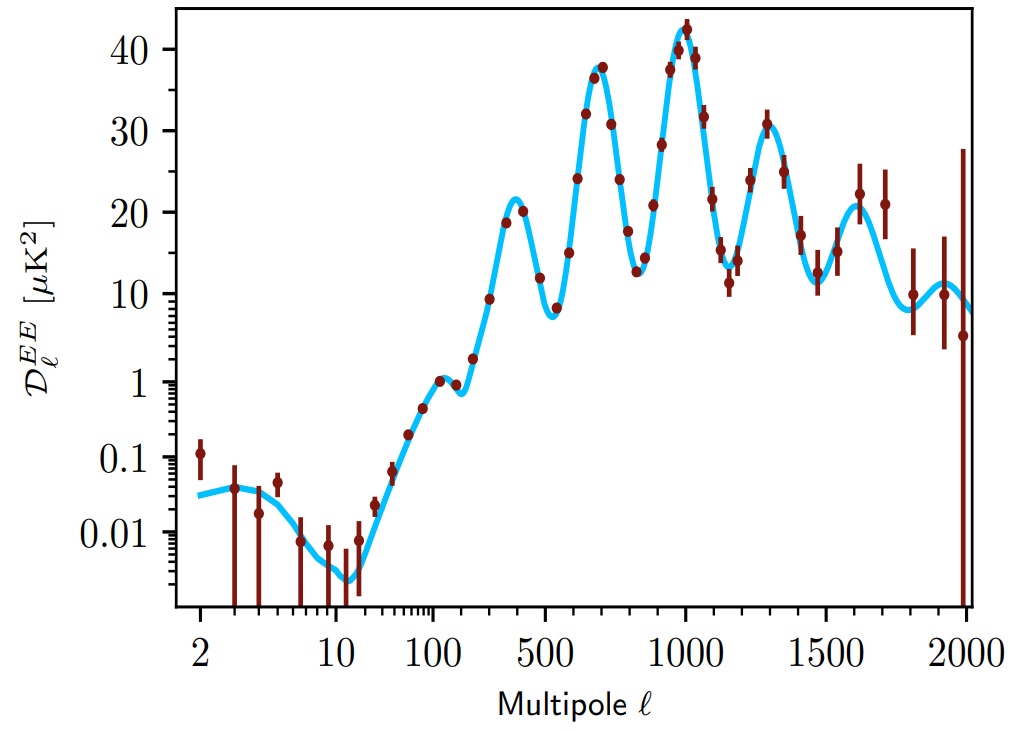
\includegraphics[width=0.45\linewidth]{ScientificMotivation/Figures/Planck_CMB_EEspectrum_2019.png}}
    }
    \hfill
    \subfloat[\label{fig:cmb_ee_spectrum:b}]{
        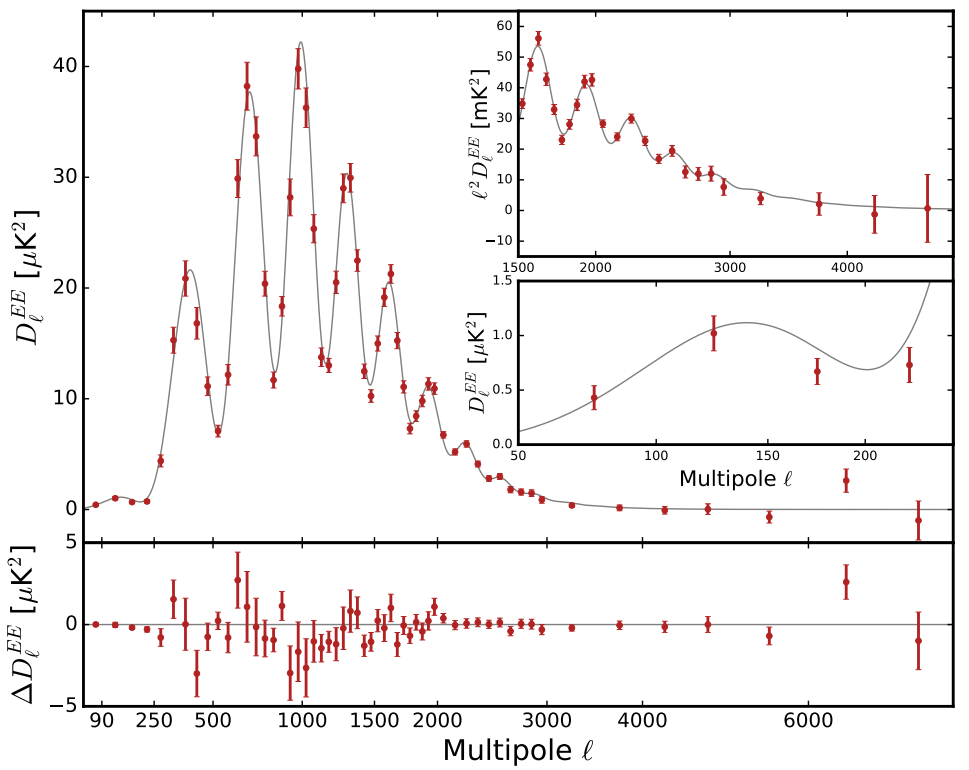
\includegraphics[width=0.51\linewidth]{ScientificMotivation/Figures/SPT_CMB_EEspectrum_2018.png}
    }
    \caption[Planck and SPT EE power spectra]{Autocorrelation power spectra of the CMB E-mode anisotropies as a function of angular scale. \ref{fig:cmb_ee_spectrum:a} shows the EE measurement presented in the Planck 2018 data release and shows exquisite agreement with the best-fit $\Lambda$CDM model to $\ell \sim 1500$ \cite{planck_collaboration_planck_2019}. \ref{fig:cmb_ee_spectrum:b} shows the EE measurement presented by the SPT collaboration in 2018, agreeing closely with the Planck spectrum at low-$\ell$ while also fitting the model well out to smaller angular scales.}
    \label{fig:cmb_ee_spectrum}
\end{figure}

\begin{figure}
    \centering
    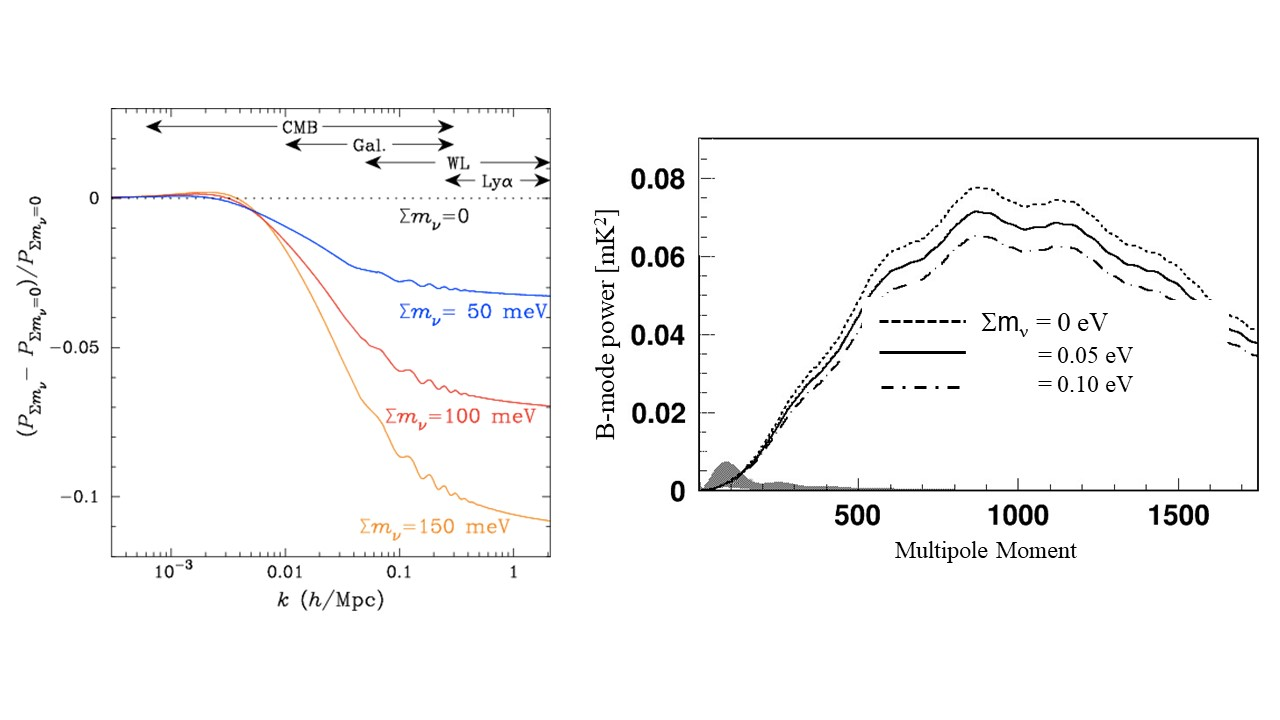
\includegraphics[width=\linewidth, trim=0cm 2cm 0cm 2cm, clip]{ScientificMotivation/Figures/neutrino_ps.jpg}
    \caption[Effect of cosmic neutrinos on the matter and CMB B-mode power spectra]{Effect of cosmic neutrinos on the matter and CMB B-mode power spectra. The figure on the left shows the fractional suppression in matter power vs neutrino mass, compared to the hypothetical case of no neutrinos. The degree of suppression is governed by the fraction of matter that sreams freely and hence smears structure on small scales. The figure on the right shows the impact of cosmic neutrinos on the CMB B-mode power spectrum. The structure suppression at these earlier times is governed by the point at which the neutrinos transition from relativistic to non-relativistic particles, which in turn impacts the physics of the early-time Integrated Sachs-Wolfe effect. The larger the neutrino mass, the earlier the universe transitions from radiation-dominated to matter-dominated, and hence the less strucutre seen in the CMB. \cite{abazajian_neutrino_2015}}
    \label{fig:neutrino_ps}
\end{figure}

\begin{figure}[!ht]
    \subfloat[\label{fig:foreground_spectra:a}]{
        \raisebox{0.5cm}{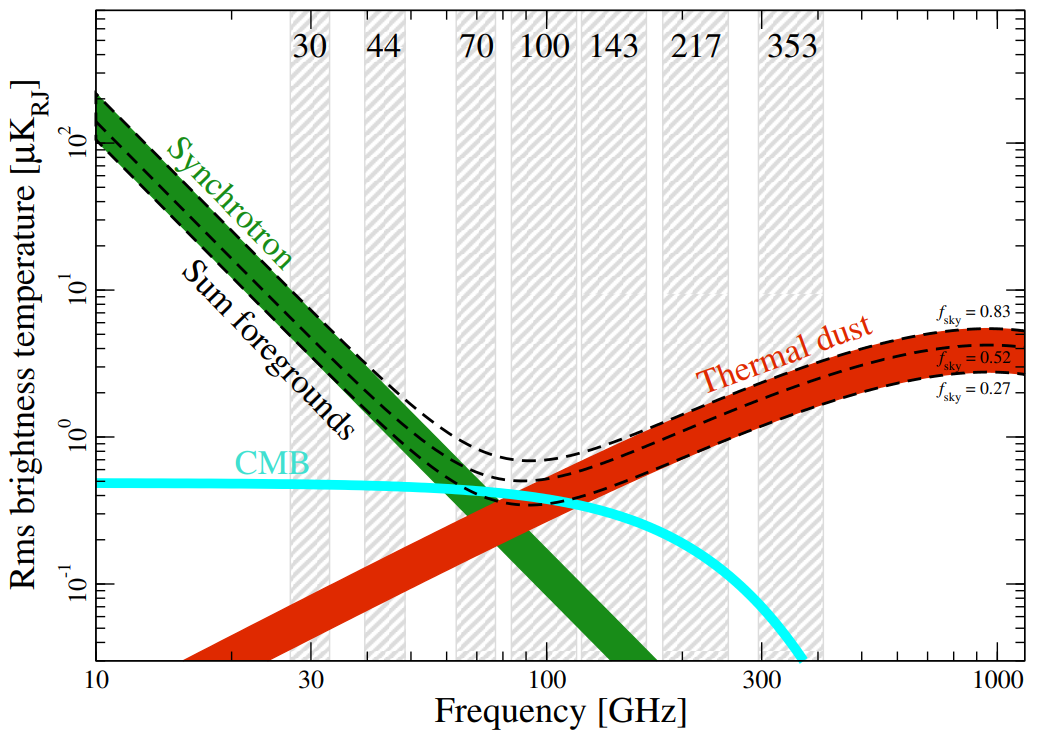
\includegraphics[width=0.45\linewidth]{ScientificMotivation/Figures/Foreground_spectrum_Planck_2019.png}}
    }
    \hfill
    \subfloat[\label{fig:foreground_spectra:b}]{
        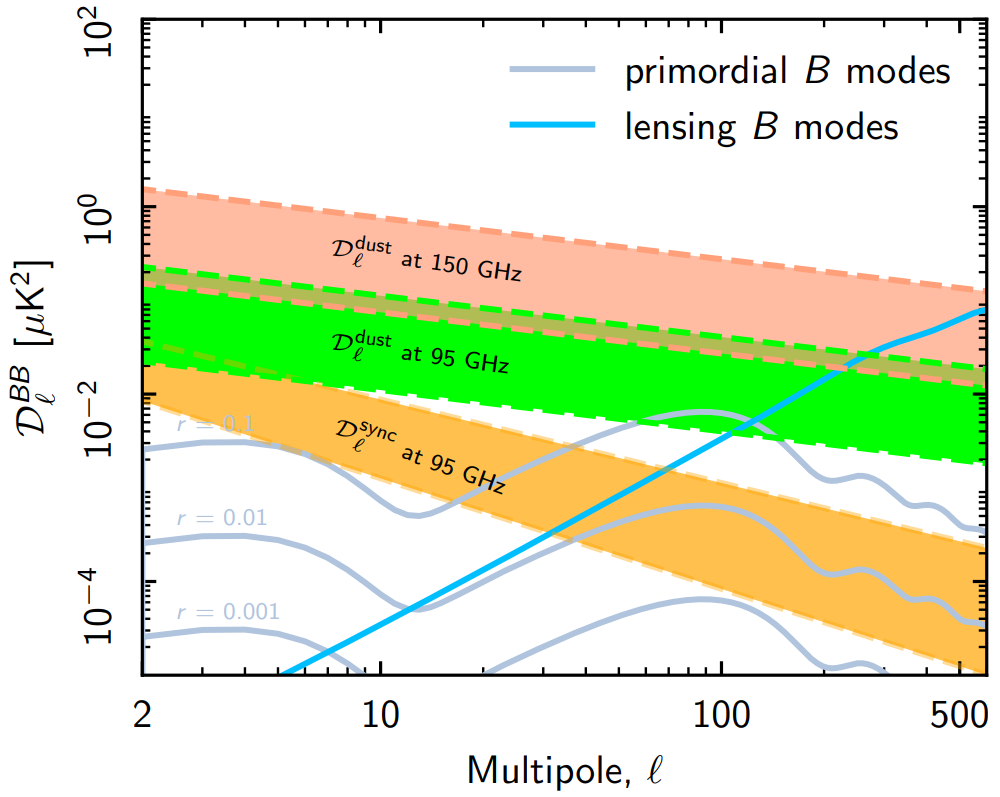
\includegraphics[width=0.45\linewidth]{ScientificMotivation/Figures/Foreground_angularSpectrum_Planck_2019.png}
    }
    \caption[Polarized foreground frequency and angular power spectra]{The intensity of polarized synchrotron and dust compared to that of the CMB. \ref{fig:foreground_spectra:a} shows spatially averaged foreground brightness vs frequency for various fractions of the sky \cite{planck_collaboration_planck_2019}. \ref{fig:foreground_spectra:b} shows the angular power spectrum of dust and synchrotron at two common CMB observation frequencies, compared to the lensing B-mode spectrum and a possible primordial B-mode spectra \cite{planck_collaboration_planck_2018}.}
    \label{fig:foreground_spectra}
\end{figure}

\section{State of the field}

\begin{figure}[!ht]
    \subfloat[\label{fig:bb_spectrum:a}]{
        \raisebox{1.1cm}{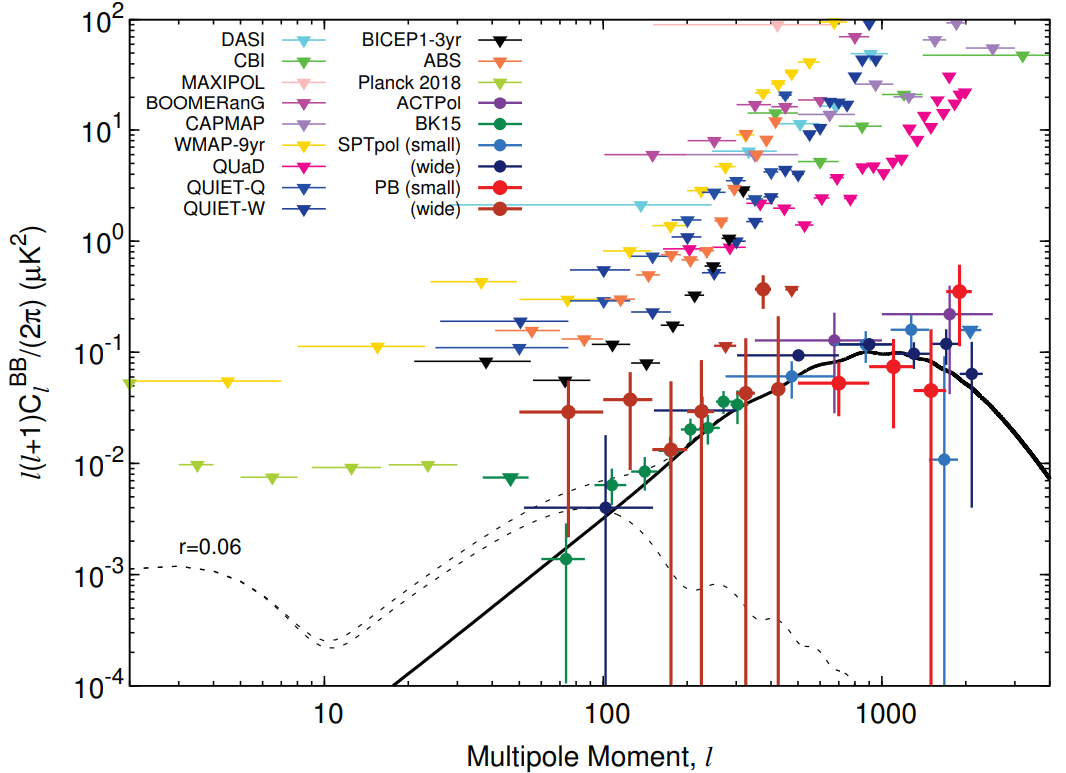
\includegraphics[width=0.45\linewidth]{ScientificMotivation/Figures/Yuji_BB_spectrum.png}}
    }
    \hfill
    \subfloat[\label{fig:bb_spectrum:b}]{
        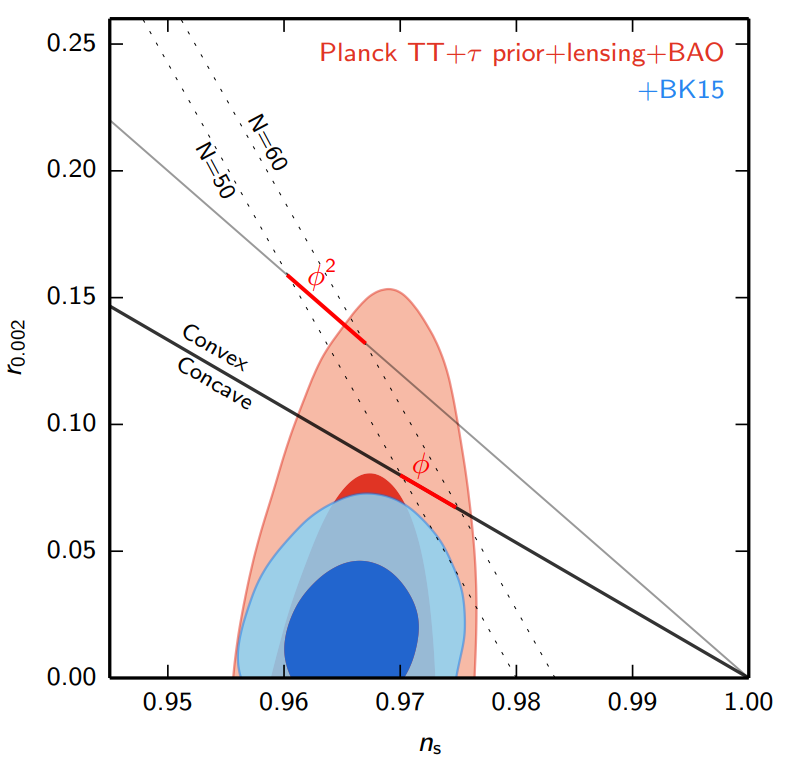
\includegraphics[width=0.45\linewidth]{ScientificMotivation/Figures/Keck_r_ns_2018.png}
    }
    \caption[Current state of the BB measurement and exclusion regions in the r vs $n_{\mathrm{s}}$ plane]{The current state of the CMB B-mode polarization autocorrelation power spectrum, as well as it implications for constraints on inflation. \ref{fig:bb_spectrum:a} shows the history of B-mode measurements made by various experiments. The triangles represent upper limits, and the circles and crosses represent central values and uncertainties, respectively. The solid line is the best-fit, foreground-subtracted lensing spectrum as determined by the latest BICEP/Keck result, and the dotted line represents the current upper bound on $r$, which parameterizes primordial gravitational waves. Figure courtesy of Dr. Yuji Chinone. \ref{fig:bb_spectrum:b} shows the exclusion contours in the $r$-$n_{\mathrm{s}}$ plane when combining data from BAO, Planck, and BICEP/Keck \cite{array_bicep2_2018}.}
    \label{fig:bb_spectrum}
\end{figure}

\chapter{CMB instrument overview}
\label{ch:cmb_instrument_overview}

One of the most powerful and prominent methods to study the Big Bang model laid out in Chapter~\ref{ch:scientific_motivation} is to study CMB temperature and polarization anisotropies with high precision. Such an endeavor requires specialized telescopes that are designed specifically to be sensitive at millimeter wavelengths. These telescopes are then used to map the CMB---or to measure its intensity and polarization fluctuations as a function of sky coordinate---by scanning its field of view across the sky.

Modern-day CMB instruments are \important{background limited}, meaning that their sensitivity is limited by fluctuations in optical signal itself, as opposed to detector or electrical noise. Given this reality, the current state of the art is deploy more detectors whose outputs can be averaged to improve signal to noise. This is in contrast to the earlier days of CMB instrumentation, which primarily invested resources to make a small number of detectors as sensitive as possible. Of course, improving per-detector sensitivity is critically important and is still an active area of research, but scaling to large detector arrays is a relatively new phenomenon that drives many of the research areas presented in this document.

In this section, we break down CMB instrumentation into three categories that are particularly relevant to the proceeding research: optics, thermal design, and detectors. The following subsections present these subsystems in the context of two CMB observatories which are most relevant to the work presented in this thesis: Simons Array and Simons Observatory.

%%%%%%%%%%%%%%%%%%%%%%%%%%%%%%%%
%%%%%%%%%%%%%%%%%%%%%%%%%%%%%%%%

\subsection{Simons Array}
\label{sec:simons_array_description}

Simons Array (SA) is a CMB observatory consisting of three identical telescopes, each with its own distinct receiver cryostat. The three receivers are called POLARBEAR-2a (PB-2a), PB-2b, and PB-2c, and their designs are reminiscent of their predecessor experiment, POLARBEAR, which observed at the SA site from 2012 to 2018. PB-2a and PB-2b have observation bands centered at 90 and 150~GHz, while PB-2c have bands at 220 and 270~GHz. Each receiver contains 1,897 dichroic (or being sensitive to two color simultaneously) detector pixels, which represents a substantial leap in both detector count and technical complexity compared to POLARBEAR.

%%%%%%%%%%%%%%%%%%%%%%%%%%%%%%%%
%%%%%%%%%%%%%%%%%%%%%%%%%%%%%%%%

\subsection{Simons Observatory}
\label{sec:simons_observatory_description}

Simons Observatory (SO) is an upcoming CMB observatory consisting of one large aperture telescope (LAT) and four small aperture telescopes (SATs). The LAT has one LAT receiver (LATR) that can house up to 13 individual optics tubes (OTs), while each small aperture telescope includes only one optics tube. Each optics tube in SO is dichroic and is one of three frequency varieties: low-frequency (LF) at 30~and~40~GHz, mid-frequency (MF) at 90~and~150~GHz, and ultra-high-frequency (UHF) at 220~and~270~GHz. 

Each LATR OT is designed to house three detector wafers, while each SAT OT is deisnge to house seven. The LAT and SAT detector wafer designs are shared between the telescopes, and the detector counts are 148 per LF wafer, and 1,728 per MF and UHF wafer. The distribution of frequencies within the LATR is discussed in Section~\ref{sec:bolocalc_informing_so_design}, but assuming two LF OTs, 8 MF OTs, and 3 UHF OTs, the LAT can hold up to $\approx$~58,000 detectors, while the SATs, assuming one LF OT, two MF OTs, and one UHF OT, can hold up to $\approx$~37,000. Therefore, SO represents a substantial advance in detector count, which in turn will lead to unprecedented sensitivity but also gives rise to unprecedented challenges regarding technological complexity.

%%%%%%%%%%%%%%%%%%%%%%%%%%%%%%%%
%%%%%%%%%%%%%%%%%%%%%%%%%%%%%%%%
%%%%%%%%%%%%%%%%%%%%%%%%%%%%%%%%

\section{Observation site}
\label{sec:observation_site}

Observing the CMB from the ground is challenging. The atmosphere both scatters and absorbs CMB radiation and forms complex structures that evolve in both time and space via non-linear processes. This reality results in a both temporally and spatially varying sky intensity that obfuscates the CMB signal. In order to limit this obfuscation, CMB observatories at high elevation, where the air is thin, and in dry conditions, where the humidity is low. In this section, we focus specifically on the observation site for SO and SA, which is located in the Atacama Desert of northeastern Chile.

%%%%%%%%%%%%%%%%%%%%%%%%%%%%%%%%
%%%%%%%%%%%%%%%%%%%%%%%%%%%%%%%%

\subsection{Sky intensity}
\label{sec:sky_intensity}

The most important parameter for an effective CMB observation site is the sky's mm-wave brightness. When discussing sky intensity, radio astronomers often refer to its ``temperature,'' which is defined as
\begin{equation}
    T_{\mathrm{eff}} = \varepsilon T_{\mathrm{phys}} \, ,
    \label{eq:sky_temperature}
\end{equation}
where $T_{\mathrm{phys}}$ is the sky's physical temperature and where $T_{\mathrm{sky}}$ is what's often called the \important{effective temperature}, or the \important{Rayleigh-Jeans temperature}. This relation is handy because in the Rayleigh-Jeans (RJ) limit where $h \nu \ll k_{\mathrm{B}} T_{\mathrm{phys}}$ and where the instrument entendue is $A \Omega = \lambda^{2}$, power and effective temperature are related as
\begin{equation}
    P_{\mathrm{RJ}} = k_{\mathrm{B}} T_{\mathrm{eff}} \Delta \nu \, ,
    \label{eq:RJ_power}
\end{equation}
where $k_{\mathrm{B}}$ is the Boltzmann constant and $\Delta \nu$ is the detection bandwidth. Atmospheric emission is a major source of mm-wave photons for ground experiment, which in turn is a major source of photon noise (see Section~blah). Additionally, atmospheric transmissivity is roughly $\eta_{\mathrm{ATM}} \approx 1 - \varepsilon_{\mathrm{ATM}}$, and therefore limiting atmospheric emission is synonymous with increasing its transparency to CMB photons. 

There are two primary constituents in the atmosphere that absorb/emit mm-wave radiation: water and oxygen. Water becomes increasingly prominent at higher frequencies, both attenuating the CMB and emitting parasitic thermal radiation, while oxygen has absorption lines that, at $\sim$~100~GHz are due to rotational quanta of the $\mathrm{H_{2}O}$ molecule. As a result, water has a broadband impact on atmospheric opacity, while oxygen has impacts which are limited to relatively narrow frequency bands. The effective temperature of the depends on the line integral of its optical depth along the telescope's line of sight, which to leading order scales as
\begin{equation}
    T_{\mathrm{ATM}} \appropto \frac{1}{\sin \theta_{\mathrm{El}}} \, ,
    \label{eq:atmospheric_brightness_elevation_dependence}
\end{equation}
where $\theta_{\mathrm{El}}$ is the elevation of the telescope's boresight above the horizon. Due to this relation, scan strategies must consider sensitivity vs. elevation when optimizing how to scan the CMB (see Section~\ref{sec:scan} for more details).

\begin{figure}[!t]
    \centering
    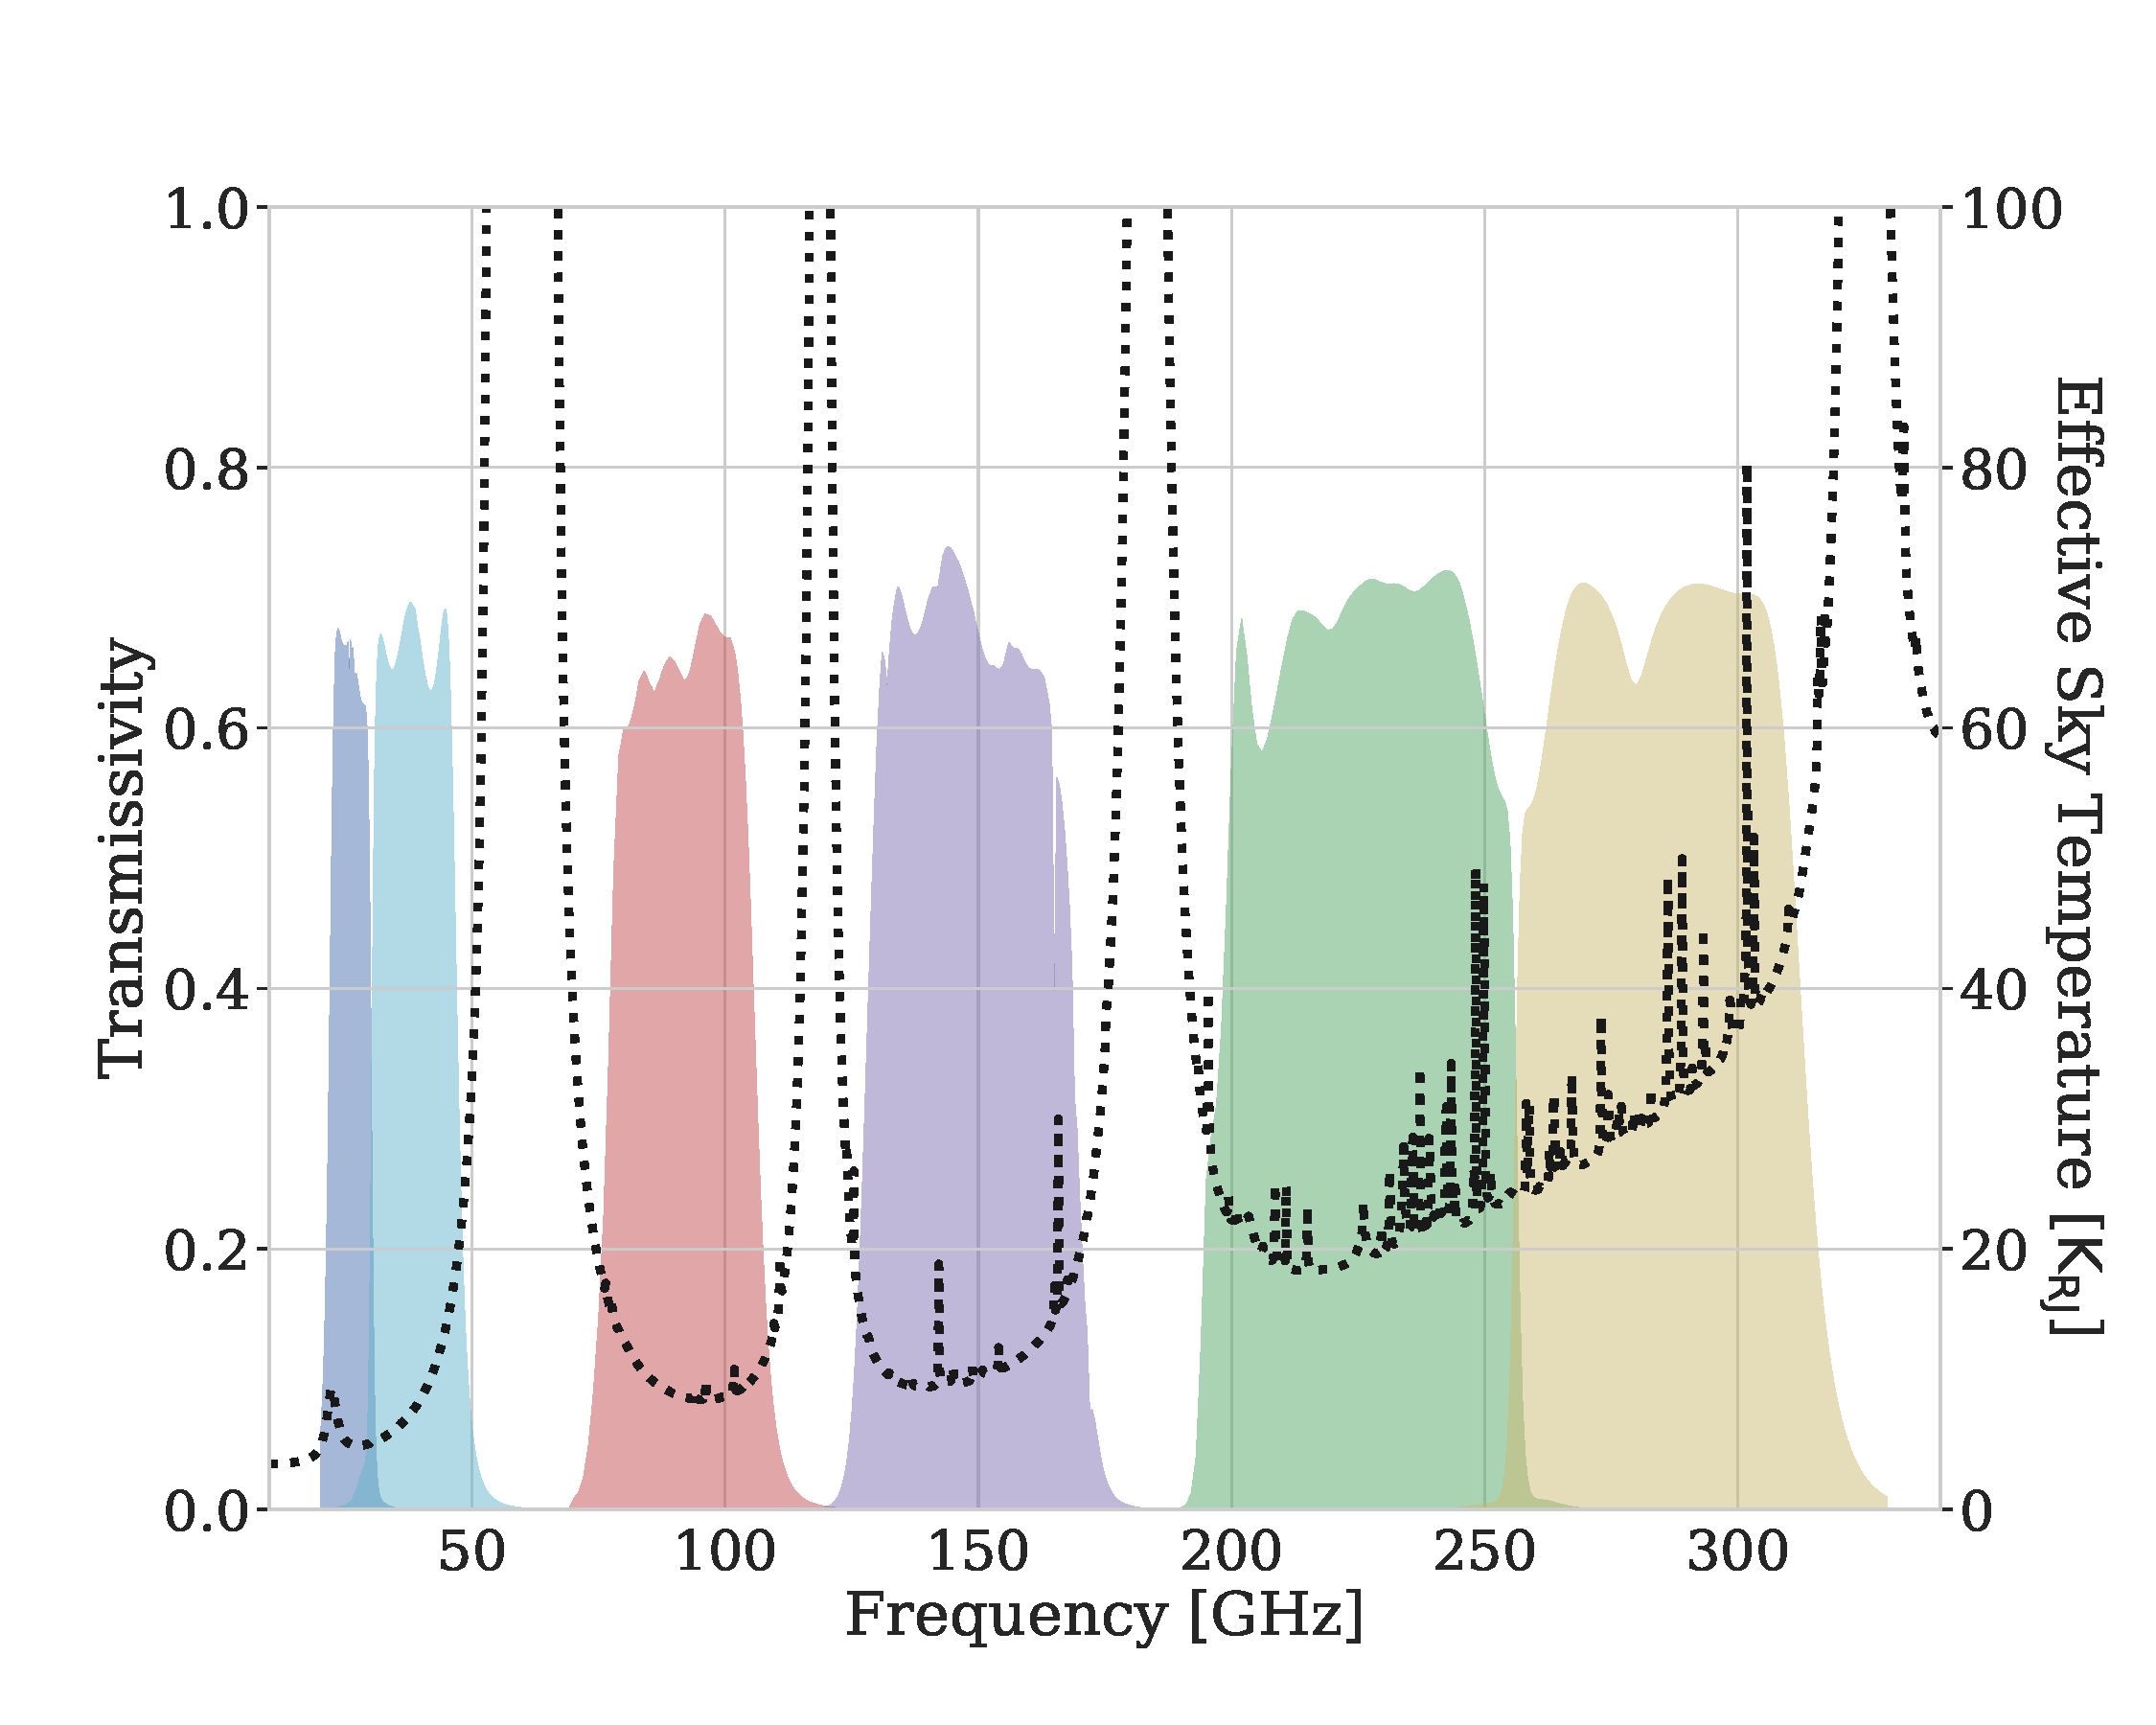
\includegraphics[width=0.8\linewidth, trim=0cm 1cm 0cm 2cm, clip]{InstrumentOverview/Figures/so_bands.pdf}
    \caption{The SO detector bands overplotted onto the Atacama sky's effective RJ temperature at 1.4~mm PWV and 50~deg elevation. The observation bands are placed in what are referred to as \important{atmospheric window} between the oxygen absorption/emission lines at $\sim$~60, 120, 180, and 330~GHz. The precipitous increase in atmospheric brightness temperature at high frequency is due to the increasing emissivity of water vapor in the far IR. This excess emission not only increases noise in the high-frequency bands but also increases the intensity the impact of atmospheric fluctuations, which makes 1/f noise mitigation challenging in the UHF bands.}
    \label{fig:so_bands_atacama}
\end{figure}

In order to quantify the amount of water in the atmosphere, we monitor the \textit{precipitable water vapor} (PWV), which is the height of liquid water equal to the amount of water vapor in an imaginary column from the ground to outer space. Emission due to water, and therefore the impact of PWV, increases with increasing frequency. To leading order, which applies reasonably well at low frequencies and small water composition, the sky intensity scales as
\begin{equation}
    T_{\mathrm{ATM}} \appropto \mathrm{PWV} \, .
    \label{eq:atmospheric_brightness_pwv_dependence}
\end{equation}
In practice, Equations~\ref{eq:atmospheric_brightness_elevation_dependence} and ~\ref{eq:atmospheric_brightness_pwv_dependence} are not used and are instead replaced by molecular simulations of the atmosphere's absorption and scattering profile, but these relations are nonetheless useful guides of water and oxygen's impact on atmospheric brightness. 

%%%%%%%%%%%%%%%%%%%%%%%%%%%%%%%%
%%%%%%%%%%%%%%%%%%%%%%%%%%%%%%%%

\subsection{Chile site}
\label{sec:sky_intensity}

\begin{figure}[!t]
    \centering
    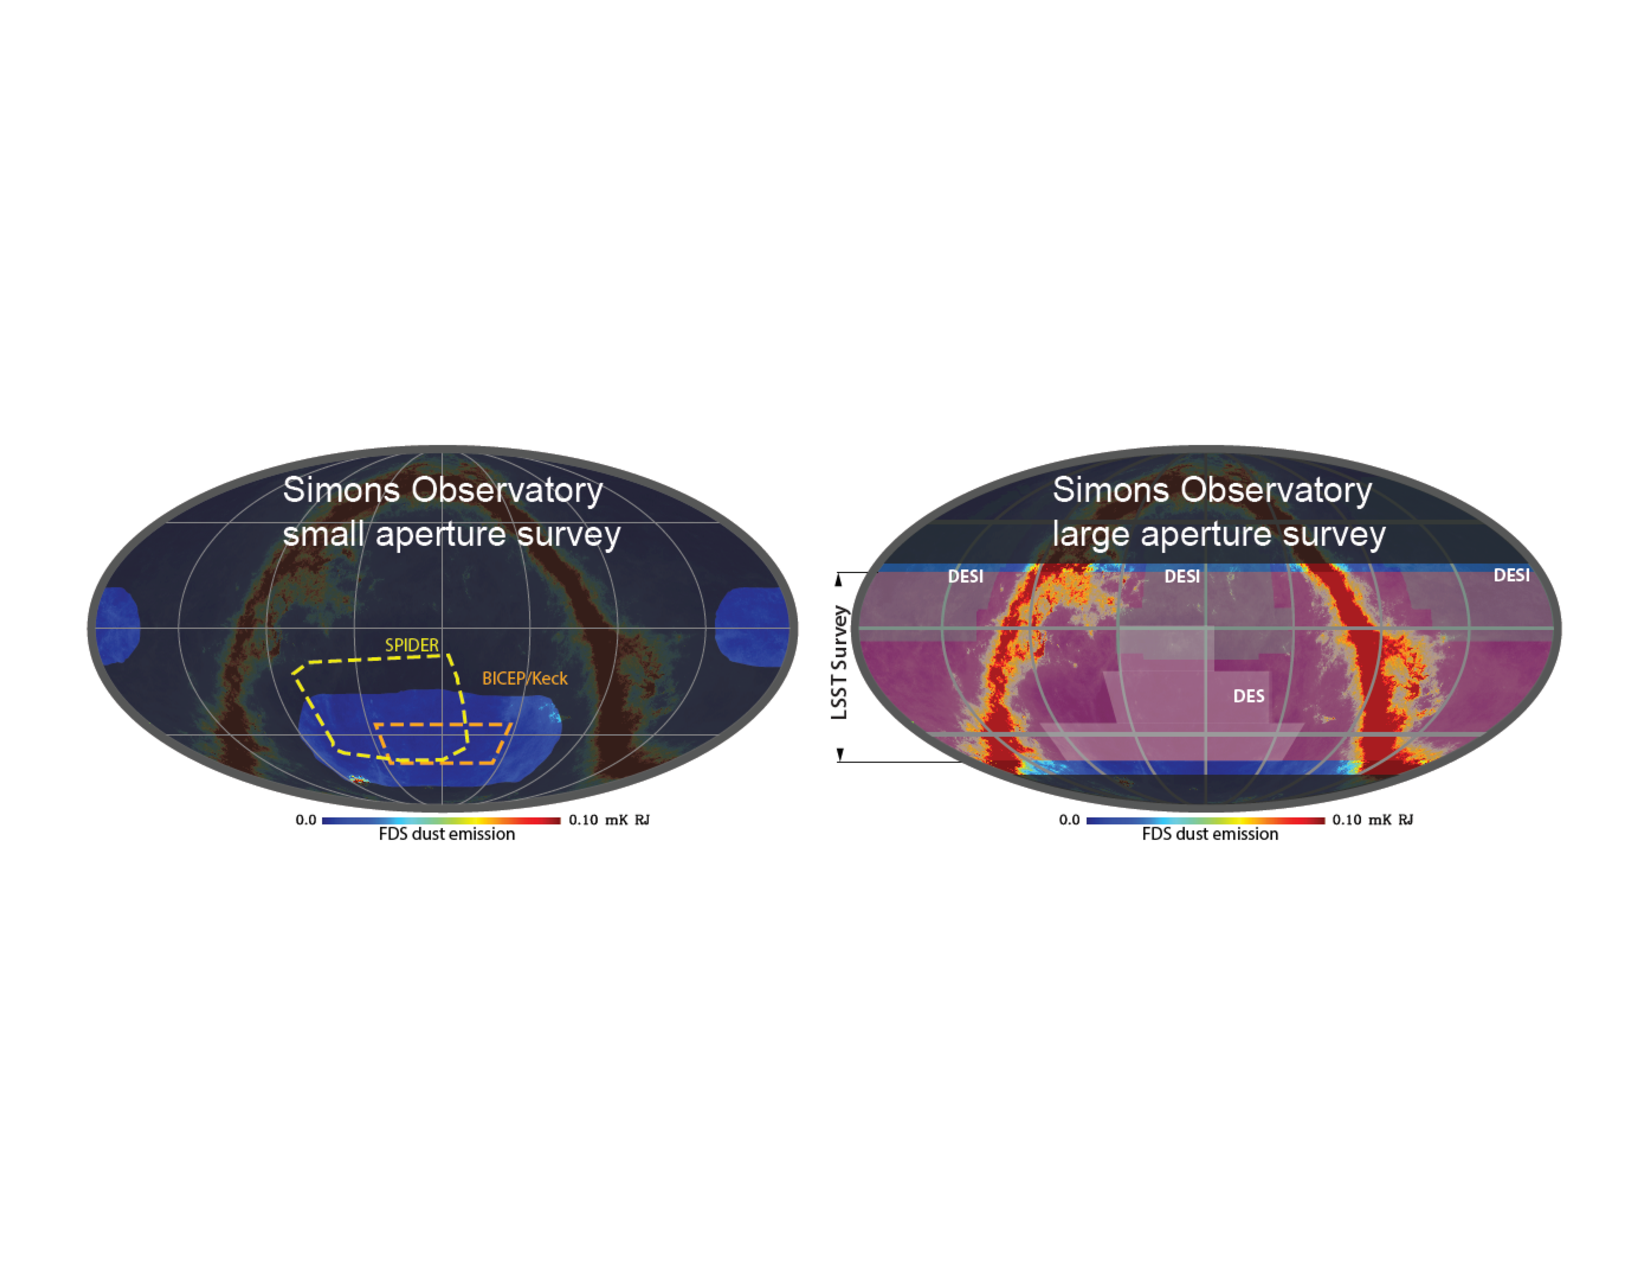
\includegraphics[width=\linewidth, trim=1cm 7cm 1cm 7cm, clip]{InstrumentOverview/Figures/so_survey.pdf}
    \caption{The LAT and SAT survey area for SO. The access to 70\% of the sky is a substantial advantage for the Atacama site compared to other sites, such as that at the South Pole.}
    \label{fig:so_survey}
\end{figure}

In order to minimize both the attenuation of the CMB and the parasitic photons due to the atmosphere, it is advantageous to observe through both as little and as dry of air as possible. The most effective approach to limit atmospheric power is to build a satellite and measure the CMB from beyond the Earth's atmosphere. While leaving Earth is certainly an effective technique to minimize the impact of its atmosphere, launching and operating a satellite costs $\sim$~billions of dollars and carries high risk, as the instrument cannot be serviced after launch. Despite these limitations, some of the most successful CMB instruments were satellite missions, including Planck and WMAP, which are discussed in Section~blah. Another effective strategy to avoid the atmosphere is to launch a high-altitude balloon, which can float at $\sim$~100,000~ft elevation, which is above $>$~99\% of the atmosphere. Though also an effective atmosphere-mitigation technique, balloons have observation lifetimes that are limited by their flight duration, and while they are much cheaper than satellites, they face the same challenges of not being able to fix the instrument after launch. For these practical reasons, observing the CMB from the ground is a competitive technique if you can do so from the right location.

\begin{figure}[!t]
    \centering
    \subfloat[\label{fig:site_photo}]{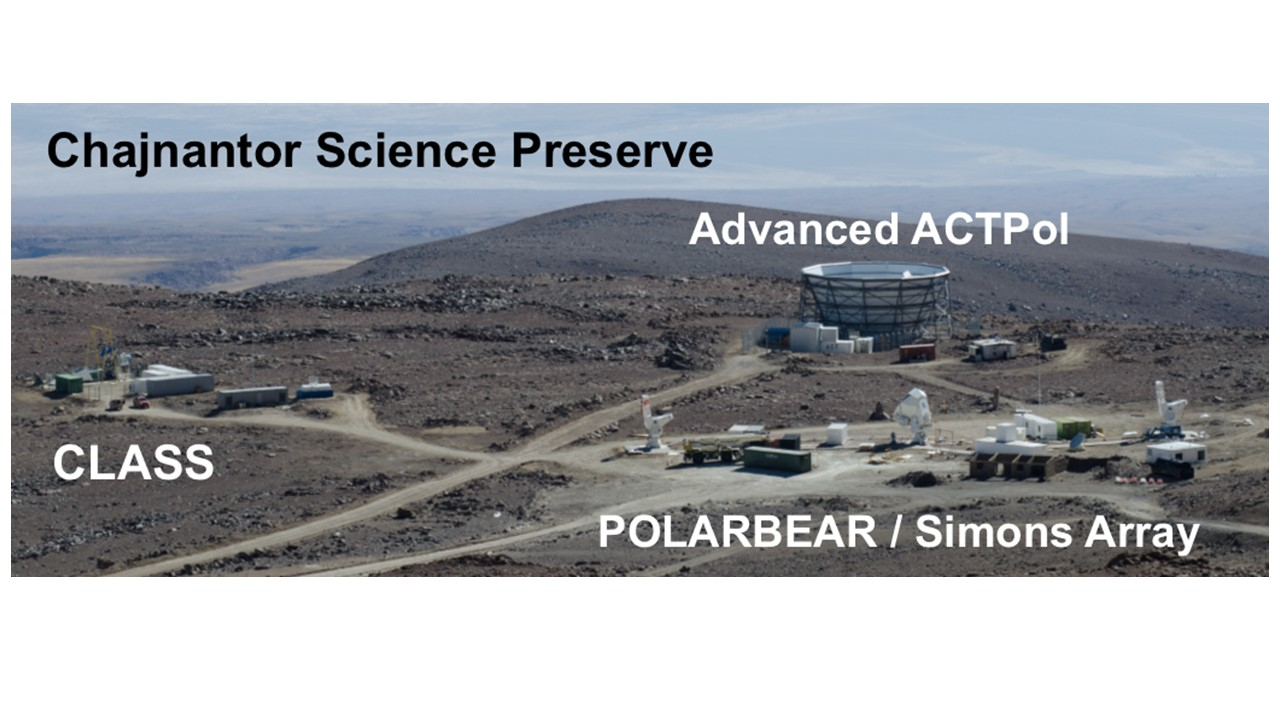
\includegraphics[width=\linewidth, trim=0cm 3.5cm 0cm 4cm clip]{InstrumentOverview/Figures/chajnantor_site.jpg}}
    \hfill
    \subfloat[\label{fig:pwv_distribution}]{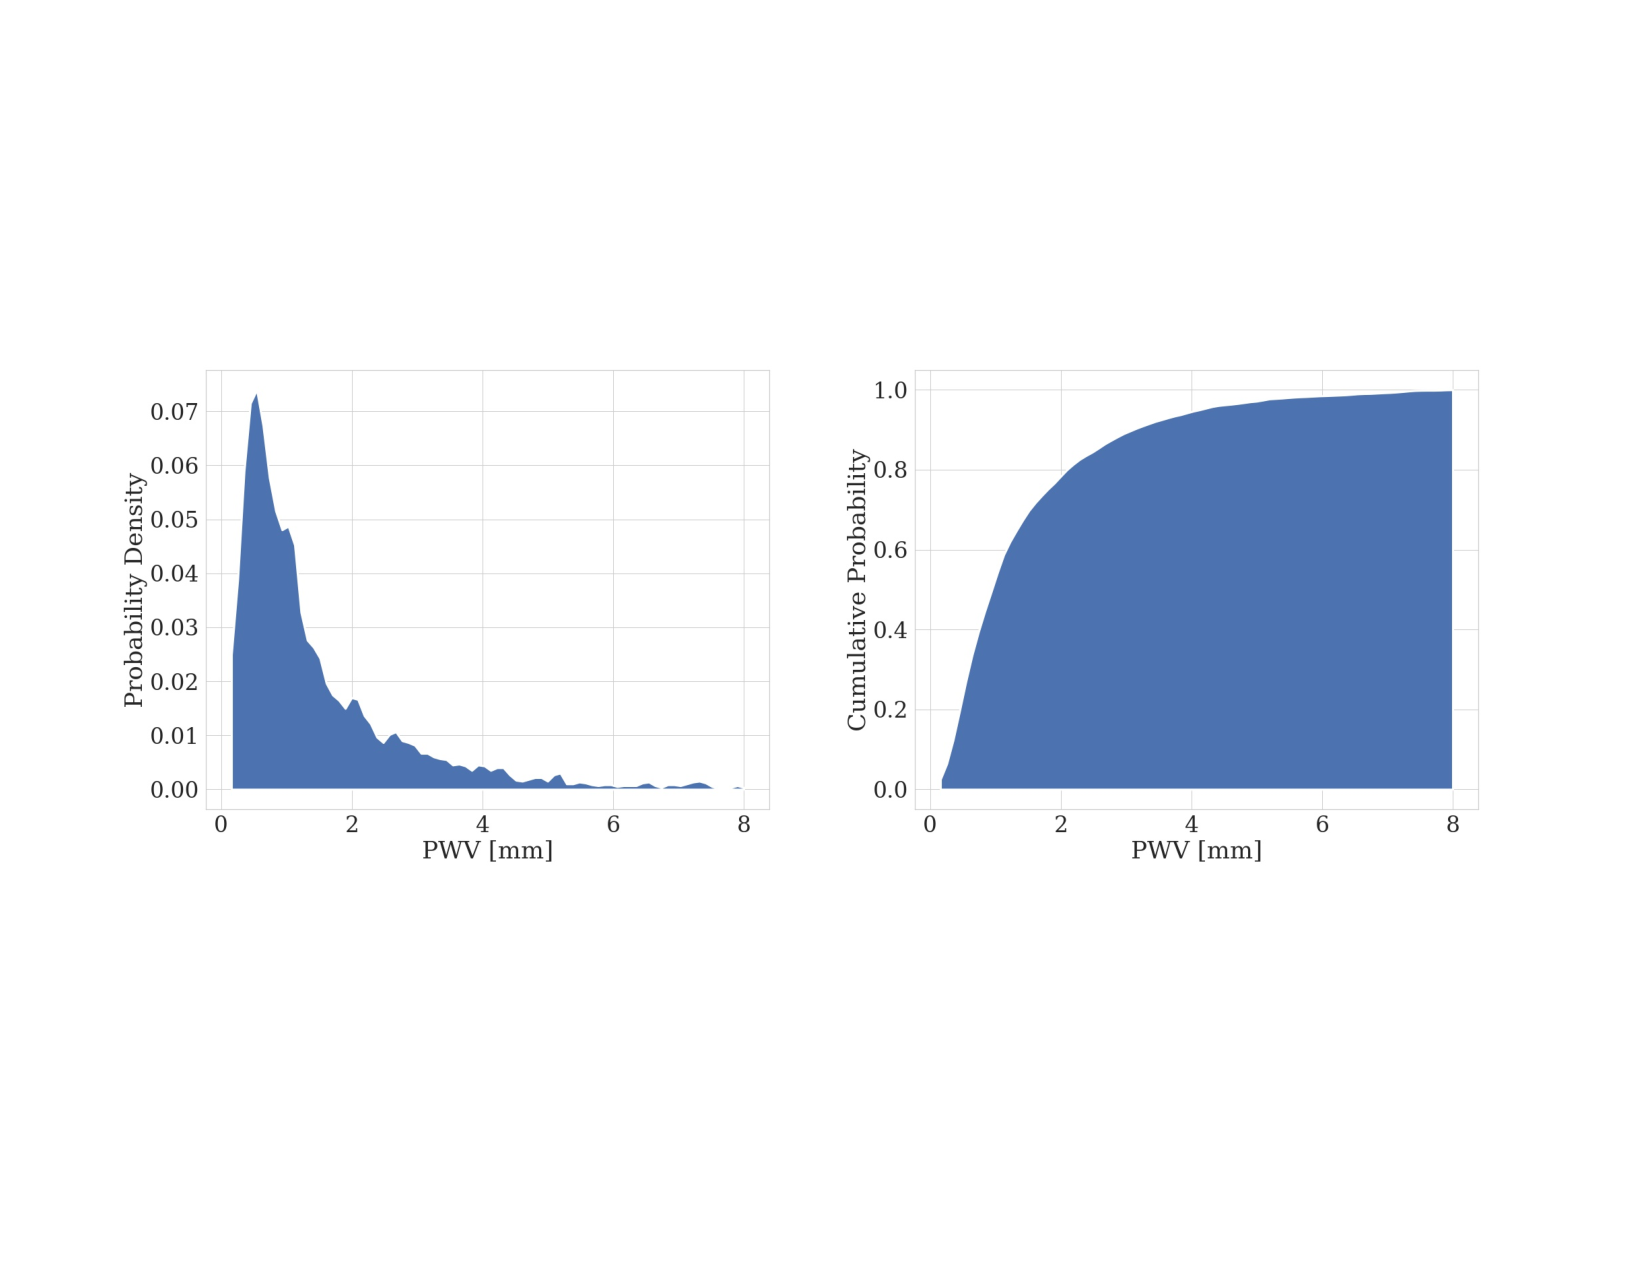
\includegraphics[width=0.95\linewidth, trim=2cm 7cm 3cm 6cm, clip]{InstrumentOverview/Figures/chile_pwv.pdf}}
    \caption[Chajnantor site]{Top panel: photograph of the observation site for Simons Array. Three PB2-style telescopes operate at 5,200 m elevation and neighbor Advanced ACT, CLASS, and Simons Observatory. PB2b operates on the southernmost of these three telescopes, which is furthest to the left. Figure courtesy of Nathan Stebor. Bottom panel: probability density and cumulative probability for PWV at the POLARBEAR-2 observation site. The median value is near 1 mm, where the value is below 2 mm nearly 80\% of the time. The dry conditions, combined with the thin atmosphere, make the Chajnantor site ideal for mm-wave astronomy observations.}
    \label{fig:pwv_distribution}
\end{figure}

Both SA and SO observe the CMB from the Chajnantor Science Preserve in the Atacama Desert of Chile on Cerro Toco. Located at 5,200~m elevation and in one of the most arid climates on Earth, Cerro Toco offers some of the best observing conditions that can be achieved terrestrially. Additionally, with its latitude of $\approx$~$-23^{\circ}$ has access to $>$~70\% of the sky, which in turn offers ample opportunity both to reduce cosmic variance by measuring a more angular modes (see Equation~\ref{eq:cosmic_variance}) and to cross correlate with other surveys. Also, because the sky rises, sets, and rotates during the course of the day in Chile, sky patches can easily be scanned in different directions---a technique called \important{cross linking}---which is a powerful tool to mitigate scan-dependent systematic errors. These last two characteristics are in contrast to another widely-used CMB observation site, the South Pole, which has access to a smaller fraction of the sky and offers no sky rotation. Figure shows the location of the Chile observation site, as well as a recent photograph of the Chilean observational site. Neighboring to SA and SO are the Atacama Cosmology Telescope (ACT) and the Cosmology Large Angular Scale Surveyor (CLASS).

Figure~\ref{fig:pwv_distribution} shows a probability distribution of the PWV during PB-1's second observation season. The median is near 1~mm, and for reference, the annual median PWV for Portland, Oregon is 20~mm, demonstrating that indeed, high-elevation, desert conditions of the Chilean observation site is indeed quite dry.

%%%%%%%%%%%%%%%%%%%%%%%%%%%%%%%%
%%%%%%%%%%%%%%%%%%%%%%%%%%%%%%%%
%%%%%%%%%%%%%%%%%%%%%%%%%%%%%%%%

\section{Optics}
\label{sec:simons_array_optics}

In its simplest form, the purpose of a CMB telescope is to image the sky onto an array of detectors with low distortion and high throughput, all while introducing minimal parasitic loading. Because 100~GHz optics are no widely available in the private sector, CMB telescopes are custom designed using unique materials that have favorable optical properties at microwave frequencies. In addition, in order to minimize photon loading, CMB optical systems are cooled to cryogenic temperatures, which both improves their transparency and limits their thermal emission. In this section, we overview the elements of the SA and SO optical systems that are relevant to the research presented in this thesis. We start by discussing SA in detail, and then we formulate a discussion of the SO optics by highlighting its differences to that of SA.

There are many figures of merit when evaluating an optical system, including field of view,  angular resolution, optical efficiency, magnification/plate scale, and (polarized) image fidelity. While each of these is important and interesting, the following subsections will focus only on what is relevant to the primary research of this thesis. 

%%%%%%%%%%%%%%%%%%%%%%%%%%%%%%%%
%%%%%%%%%%%%%%%%%%%%%%%%%%%%%%%%

\subsection{Telescope and receiver optics}
\label{sec:telescope_optics}

The SA telescope is shown as part of Figure~\ref{fig:pb2_telescope} and is composed of two monolithic mirrors that together form an off-axis Gregorian configuration. The primary mirror is a parabolic reflector that focuses incoming parallel rays onto the \textit{prime focus}. The image at prime focus is diffraction limited over only a small field of view and is therefore reimaged by an ellipsoidal secondary mirror onto the \textit{Gregorian focus}. While improved with respect to that of the primary mirror, this focus is not telecentric and still has only a moderate diffraction-limited field of view (FOV), and therefore a \textit{receiver cryostat} (also often referred to as the \textit{camera}) is employed to reimage the telescope image onto the detector array. The telescope mirrors are part of a compact telescope assembly, a photo of which is shown in Figure~\ref{fig:pb2_telescope}, which is designed to be nimble in order to enable more flexibility (speed, acceleration, elevation range, etc.) in how sky patches are scanned.

The advantages of the off-axis Gregorian design are its compactness and its satisfying the \important{Mizuguchi-Dragone} condition, which limits cross polarization by correcting any polarization rotation on the primary mirror with the secondary. The disadvantages of the SA telescope are that its mirrors are at ambient temperatures, which necessitates tight control of stray light to limit the number of 300~K photons that travel into the receiver, and that the off-axis design induces intensity to polarization (I-to-P) leakage along the y direction due to the finite conductivity of the mirror's metal, which is a systematic effect that must be subtracted from the detector data.

The SA receiver cryostat, which is also shown in Figure~\ref{fig:pb2_telescope}, contains three reimaging lenses: the field lens, aperture lens, and collimator lens. The field lens is effectively responsible for adjusting the speed of the optics at secondary focus, while the aperture and collimator lenses form an image of the primary mirror at the \textit{Lyot stop} while also forming a high-fidelity, telecentric, large-field-of-view sky image at the focal plane. All three lenses are made of alumina, which is sintered/amorphous aluminum oxide $\mathrm{Al_{2}O_{3}}$ with a high index or refraction in mm-wave ($n \approx 3.1$), and are cooled to $\approx$~4~K.

\begin{figure}
    \centering
    \subfloat[\label{fig:pb2_telescope_photo}]{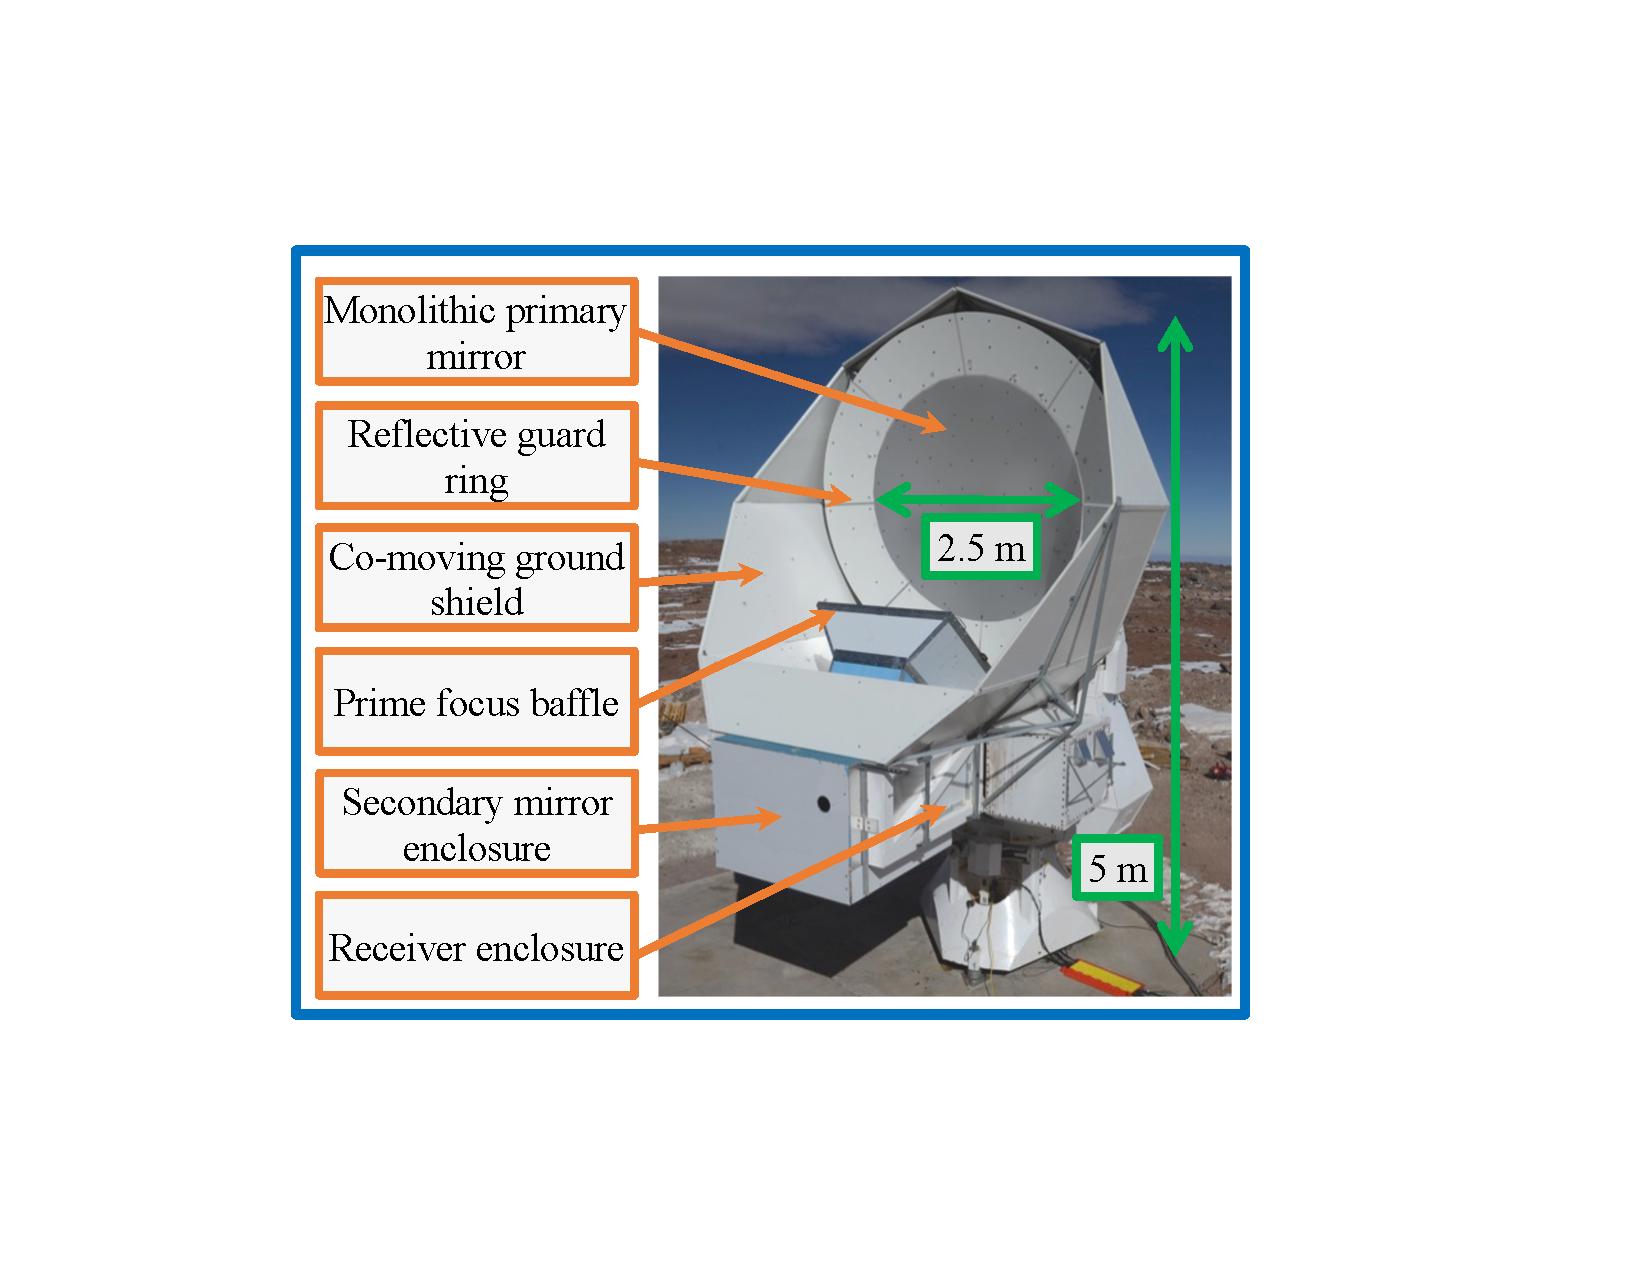
\includegraphics[width=0.9\linewidth, trim=0cm 4cm 0.5cm 4cm, clip]{InstrumentOverview/Figures/PB2b_telescope.pdf}}
    \hfill
    \subfloat[\label{fig:pb2_telescope_cad}]{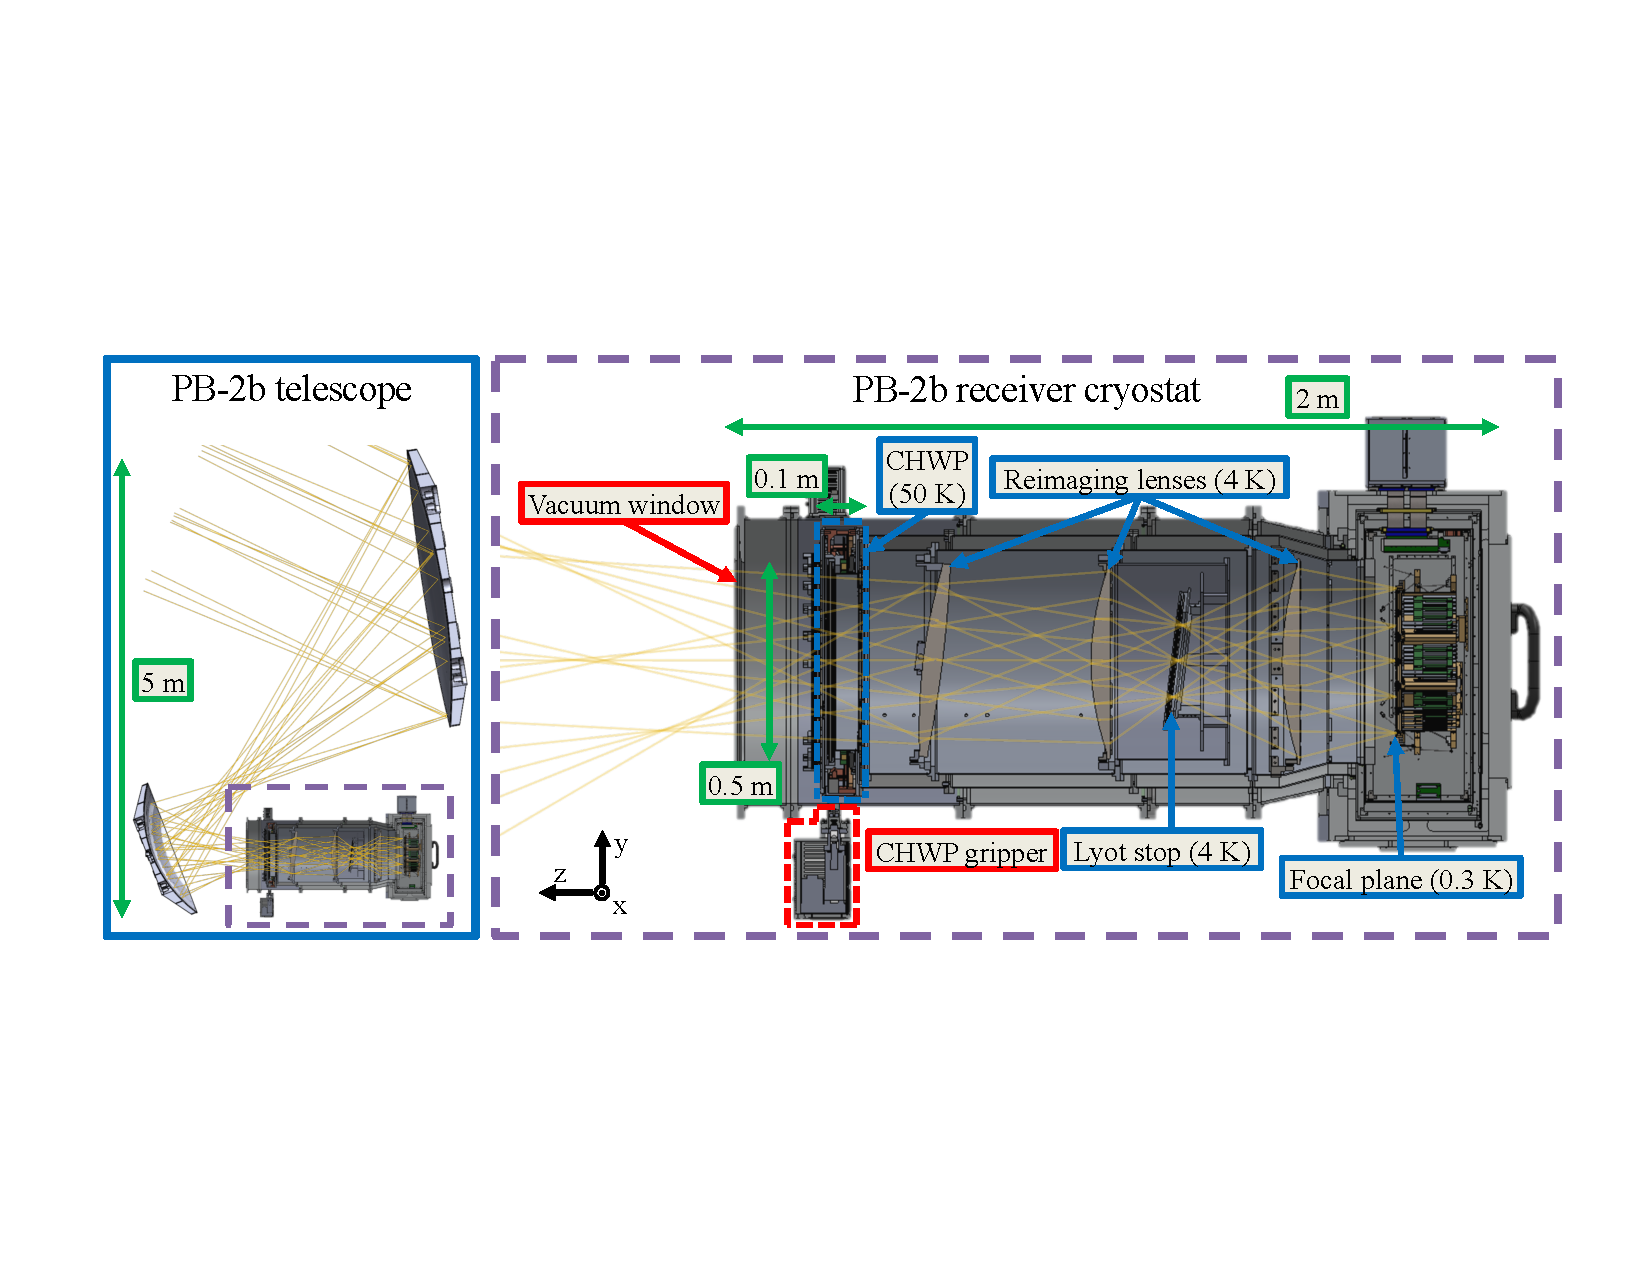
\includegraphics[width=\linewidth, trim=1.5cm 5.5cm 1.5cm 6cm, clip]{InstrumentOverview/Figures/PB2b_telescope_receiver.pdf}}
    \caption[POLARBEAR-2 telescope]{Photograph of the POLARBEAR-2 telescope. The primary and secondary mirros for an off-axis Gregorian pair. The primary reflector has a diameter of 3 m, which provides arcminute-scale angular resolution, but the compact design allows for relatively easy telescope motion. This unique combination of a large reflector and compact telescope provides POLARBEAR-2 with observational versatiliy.}
    \label{fig:pb2_telescope}
\end{figure}

The SO telescopes are shown in Figure~\ref{fig:so_telescope} and are of two varieties: a large-aperture telescope (LAT) and a small-aperture telescope (SAT). The LAT is composed of two paneled mirrors (not monolithic) which together form a crossed Dragone configuration. While less compact than the off-axis Gregorian that SA uses, the crossed Dragone (CD) offers many appealing optical properties, including outstanding image quality over a large field of view. For this reason, some small aperture telescopes in the CMB field use a CD optical system re-imaging optics. SO does, however, employ the LAT receiver cryostat (LATR) to re-image the LAT focus onto an array of up to 13 discrete focal planes, each with its own optics tube (OT). In order to push the limits of the FOV, each optics tube uses an alumina wedge that corrects the wavefront at the start of each OT such that the chief ray is approximately parallel to each OT's boresight. Then, three silicon reimaging lenses at 1~$\sim$~4~K re-image onto a detector array, through a Lyot stop, in a similar manner to the SA receiver.

The SO SAT is designed only to measure large-angular-scale CMB fluctuations, and therefore it has a smaller aperture than that of the SA and SO large-aperture telescopes. Its aperture stop is at $\sim$~2~K and is located near the vacuum window. The imaging optics comprise three silicon lenses at 1~$\sim$~2~K which image onto a $\approx$~400~mm diameter focal plane. This simpler design is much cheaper than the LAT, enabling four SATs to be constructed and operated in parallel.

\begin{figure}
    \centering
    \subfloat[\label{fig:lat_cad}]{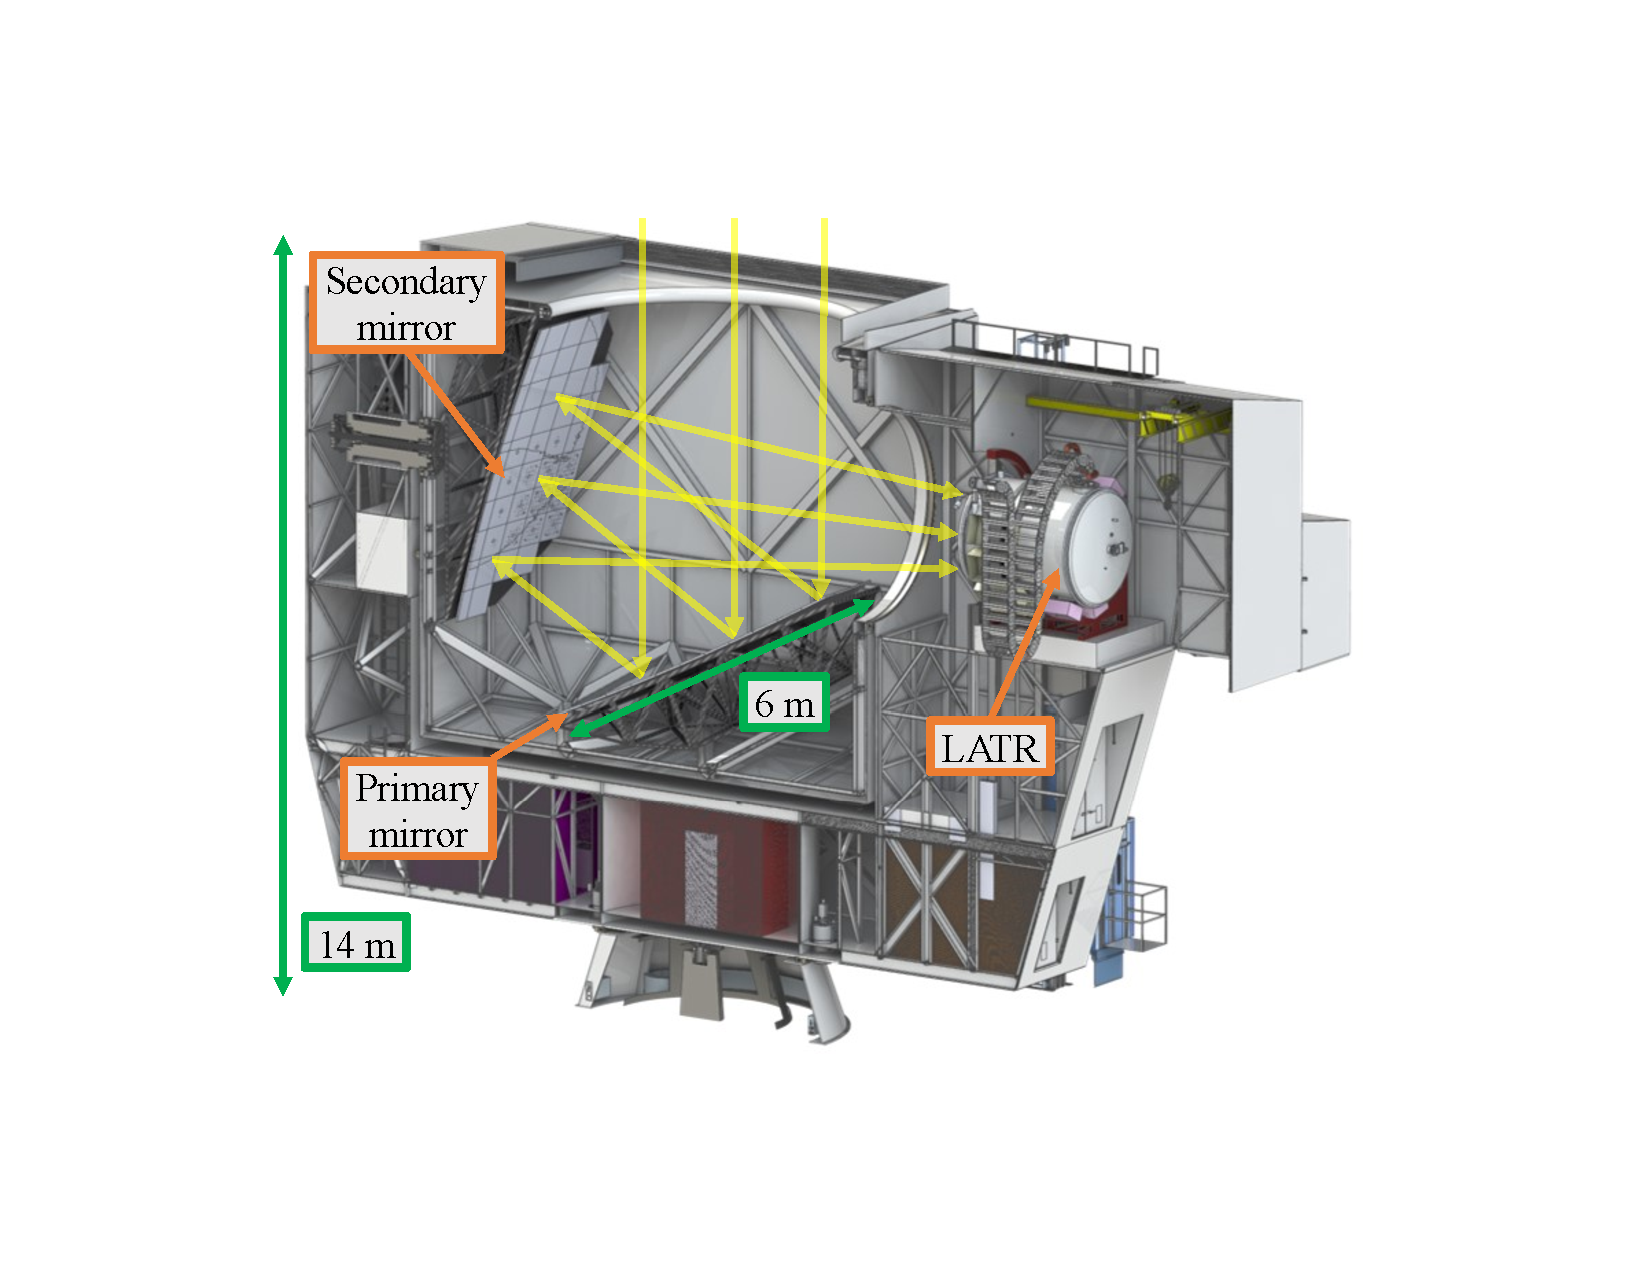
\includegraphics[width=0.7\linewidth, trim=3cm 3cm 3cm 3cm, clip]{InstrumentOverview/Figures/lat_cad.pdf}}
    \hfill
    \subfloat[\label{fig:lat_cad}]{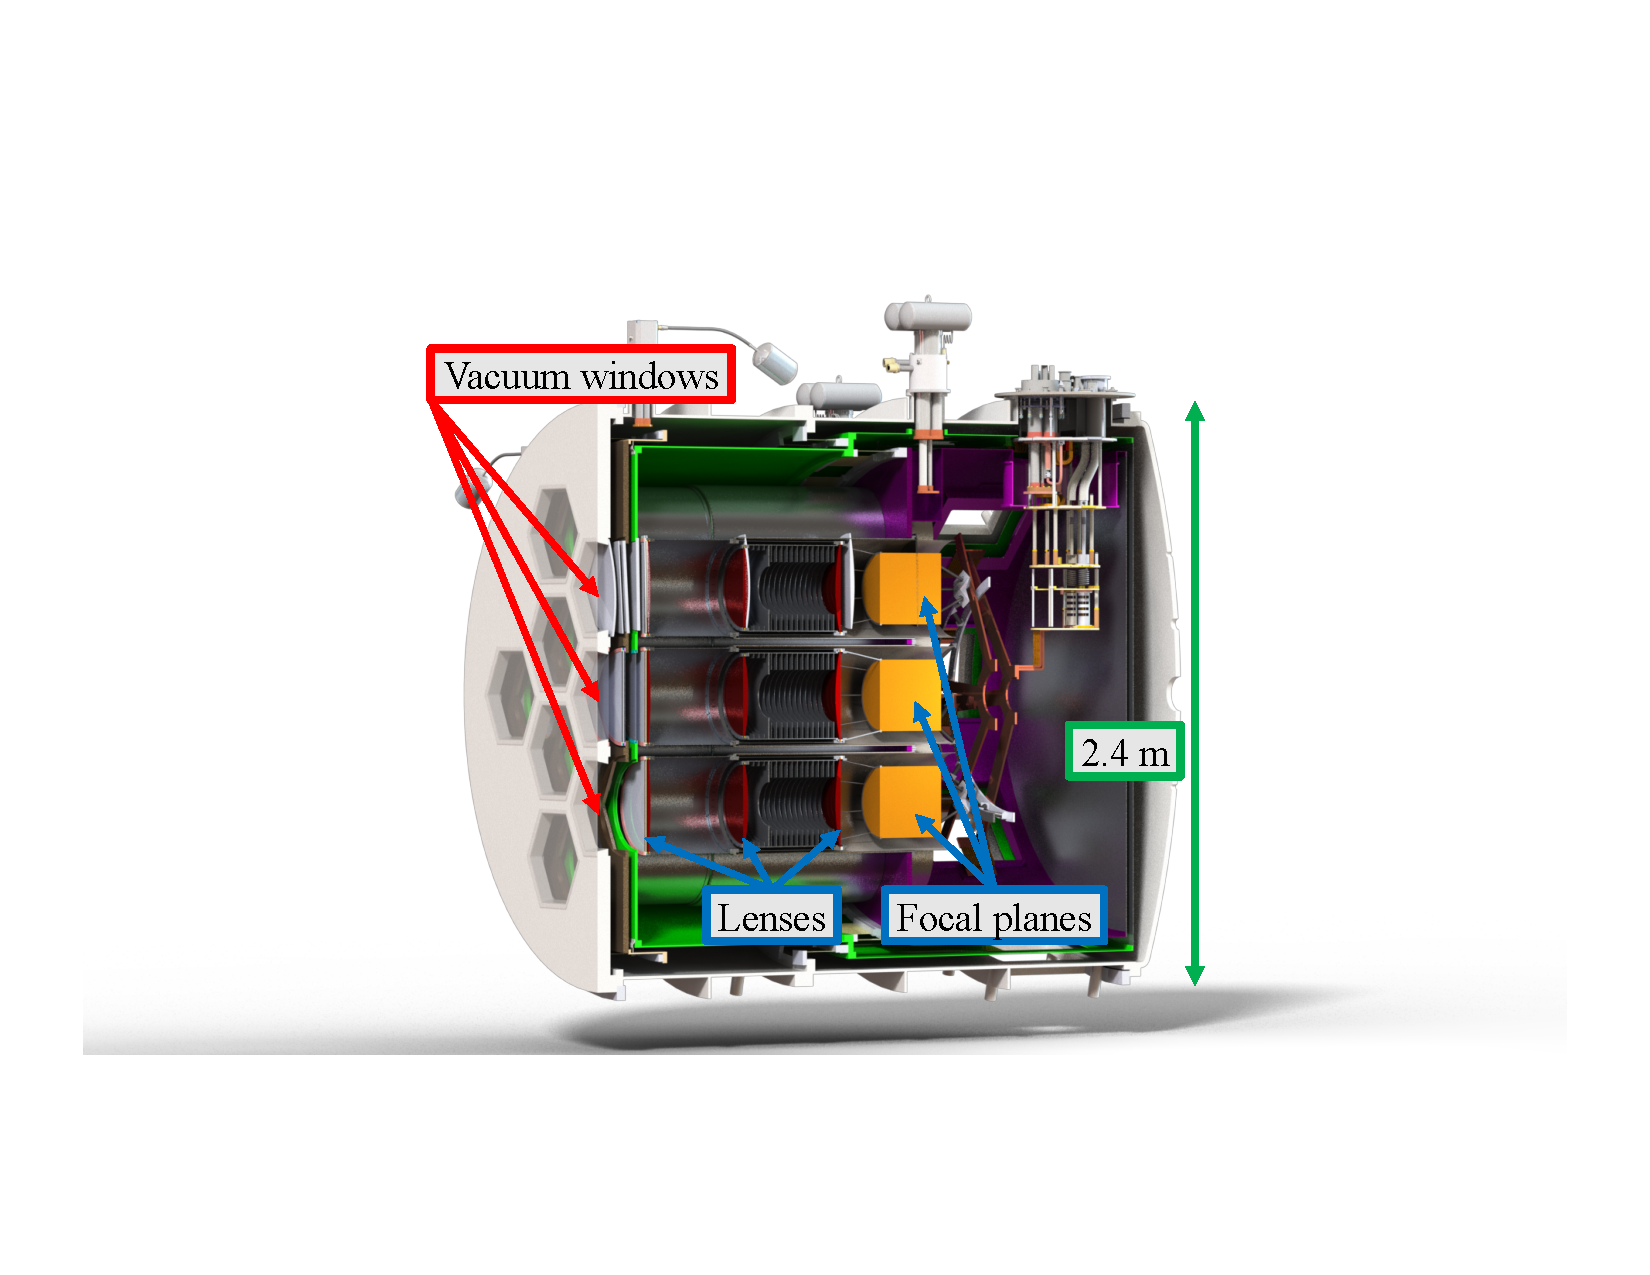
\includegraphics[width=0.5\linewidth, trim=7cm 4cm 7cm 5cm, clip]{InstrumentOverview/Figures/latr_cad.pdf}}
    \subfloat[\label{fig:lat_cad}]{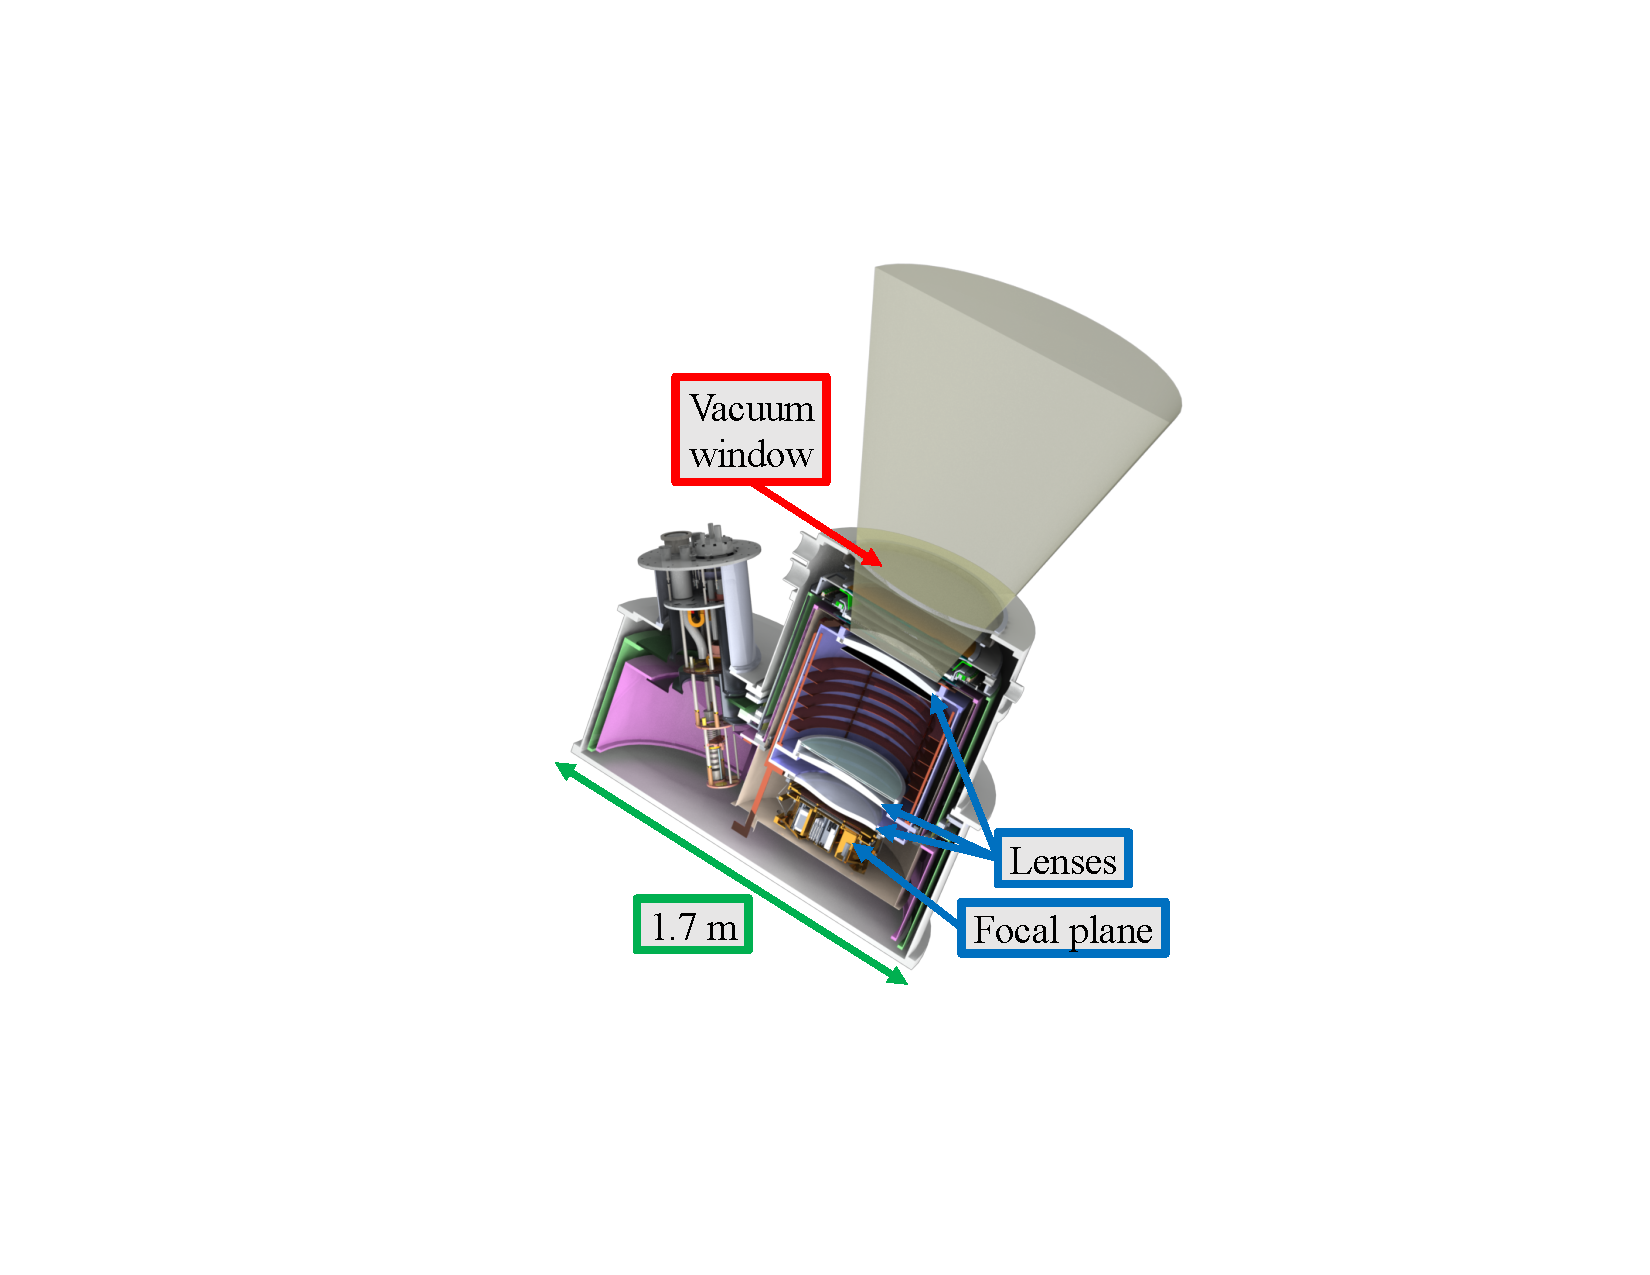
\includegraphics[width=0.5\linewidth, trim=7cm 5cm 7cm 4cm, clip]{InstrumentOverview/Figures/sat_cad.pdf}}
    \caption{Caption}
    \label{fig:so_telescope}
\end{figure}

All SA receivers and all SO SATs employ sapphire continuously-rotating half-wave plate (HWP) polarization modulators. The SA HWPs are located near the receiver's vacuum window, which is near the telescopes Gregorian focus, while the SO SAT HWPs are located directly in front of the aperture stop. HWPs are are a powerful tool to modulate sky polarization while rejecting the unpolarized atmosphere, which in turn suppresses atmospheric low-frequency noise and enables improved sensitivity to large angular scale modes. HWPs are a central research topic of this thesis document, and therefore we forego details here for a comprehensive discussion in Chapters~blah.

The most important shared characteristics of the SA and SO telescopes systems is that they are diffraction limited and FOV limited, that each receiver and optics tube images the sky onto the focal plane with high image fidelity and telecentricity, and that the diffraction-limited throughput of the system is limited by the aperture stop (or, more specifically for the SA and SO LAT, the Lyot stop). These properties are underlying assumptions for many of the calculations in Chapters to follow and are a good approximation for the presented telescope designs.

%%%%%%%%%%%%%%%%%%%%%%%%%%%%%%%%
%%%%%%%%%%%%%%%%%%%%%%%%%%%%%%%%

\subsection{Focal plane optics}
\label{sec:focal_plane_optics}

As discussed in the previous section, the telescope and receiver cryostat optics image the sky onto a focal plane. The job of the focal plane optics is to then couple the telescope image to detectors. The focal plane is comprised of discrete \important{detector pixels}, each of which is sensitive to two polarizations and two colors. PB-2a, PB-2b, two SATs, and some LAT OTs observe at 90 and 150~GHz (MF), PB-2c, one SAT, and some other LAT OTs observe at 220 and 270~GHz (UHF), and one SAT and the remaining LAT OTs observe at 30 and 40~GHz (LF).  Given this configuration, the goal of the focal plane optics is to achieve high throughput across broad bandwidths while also limiting out-of-band power.

\begin{figure}[!t]
    \centering
    \subfloat[\label{fig:focal_plane_optics:a}]{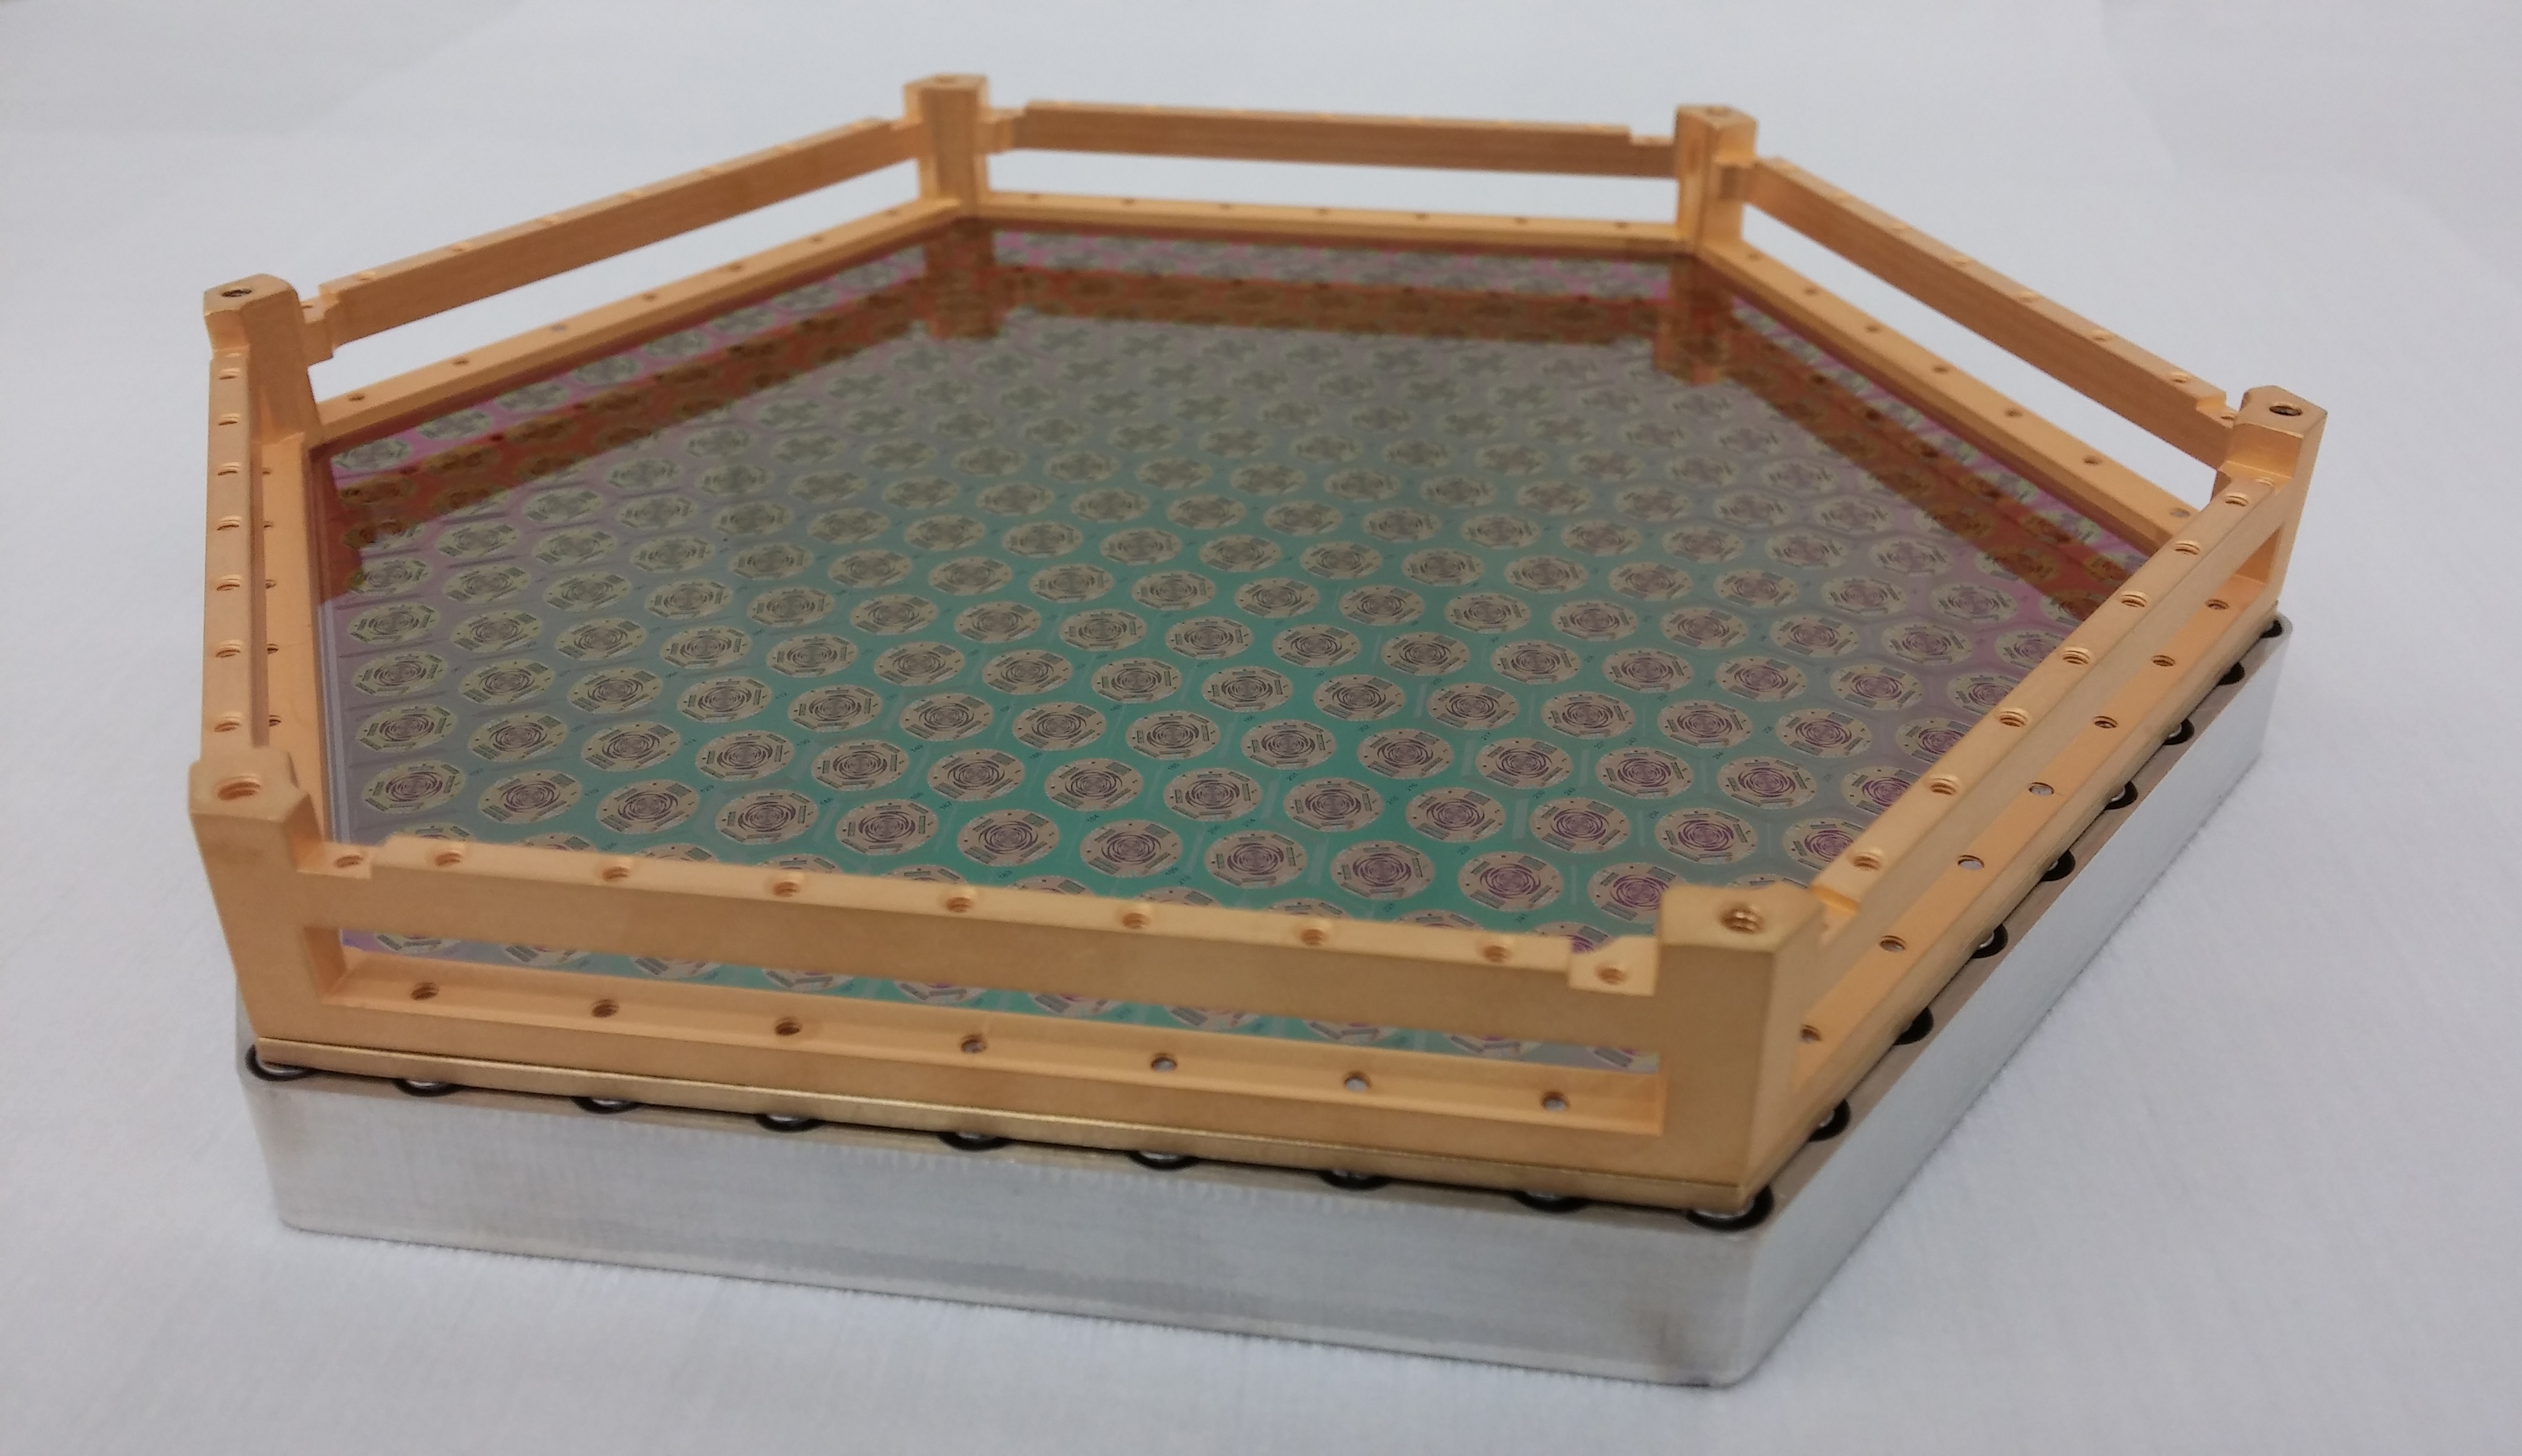
\includegraphics[width=0.48\linewidth, trim=0cm 0cm 0cm -0.2cm, clip]{InstrumentOverview/Figures/PB2_antennas.jpg}}
    \subfloat[\label{fig:focal_plane_optics:b}]{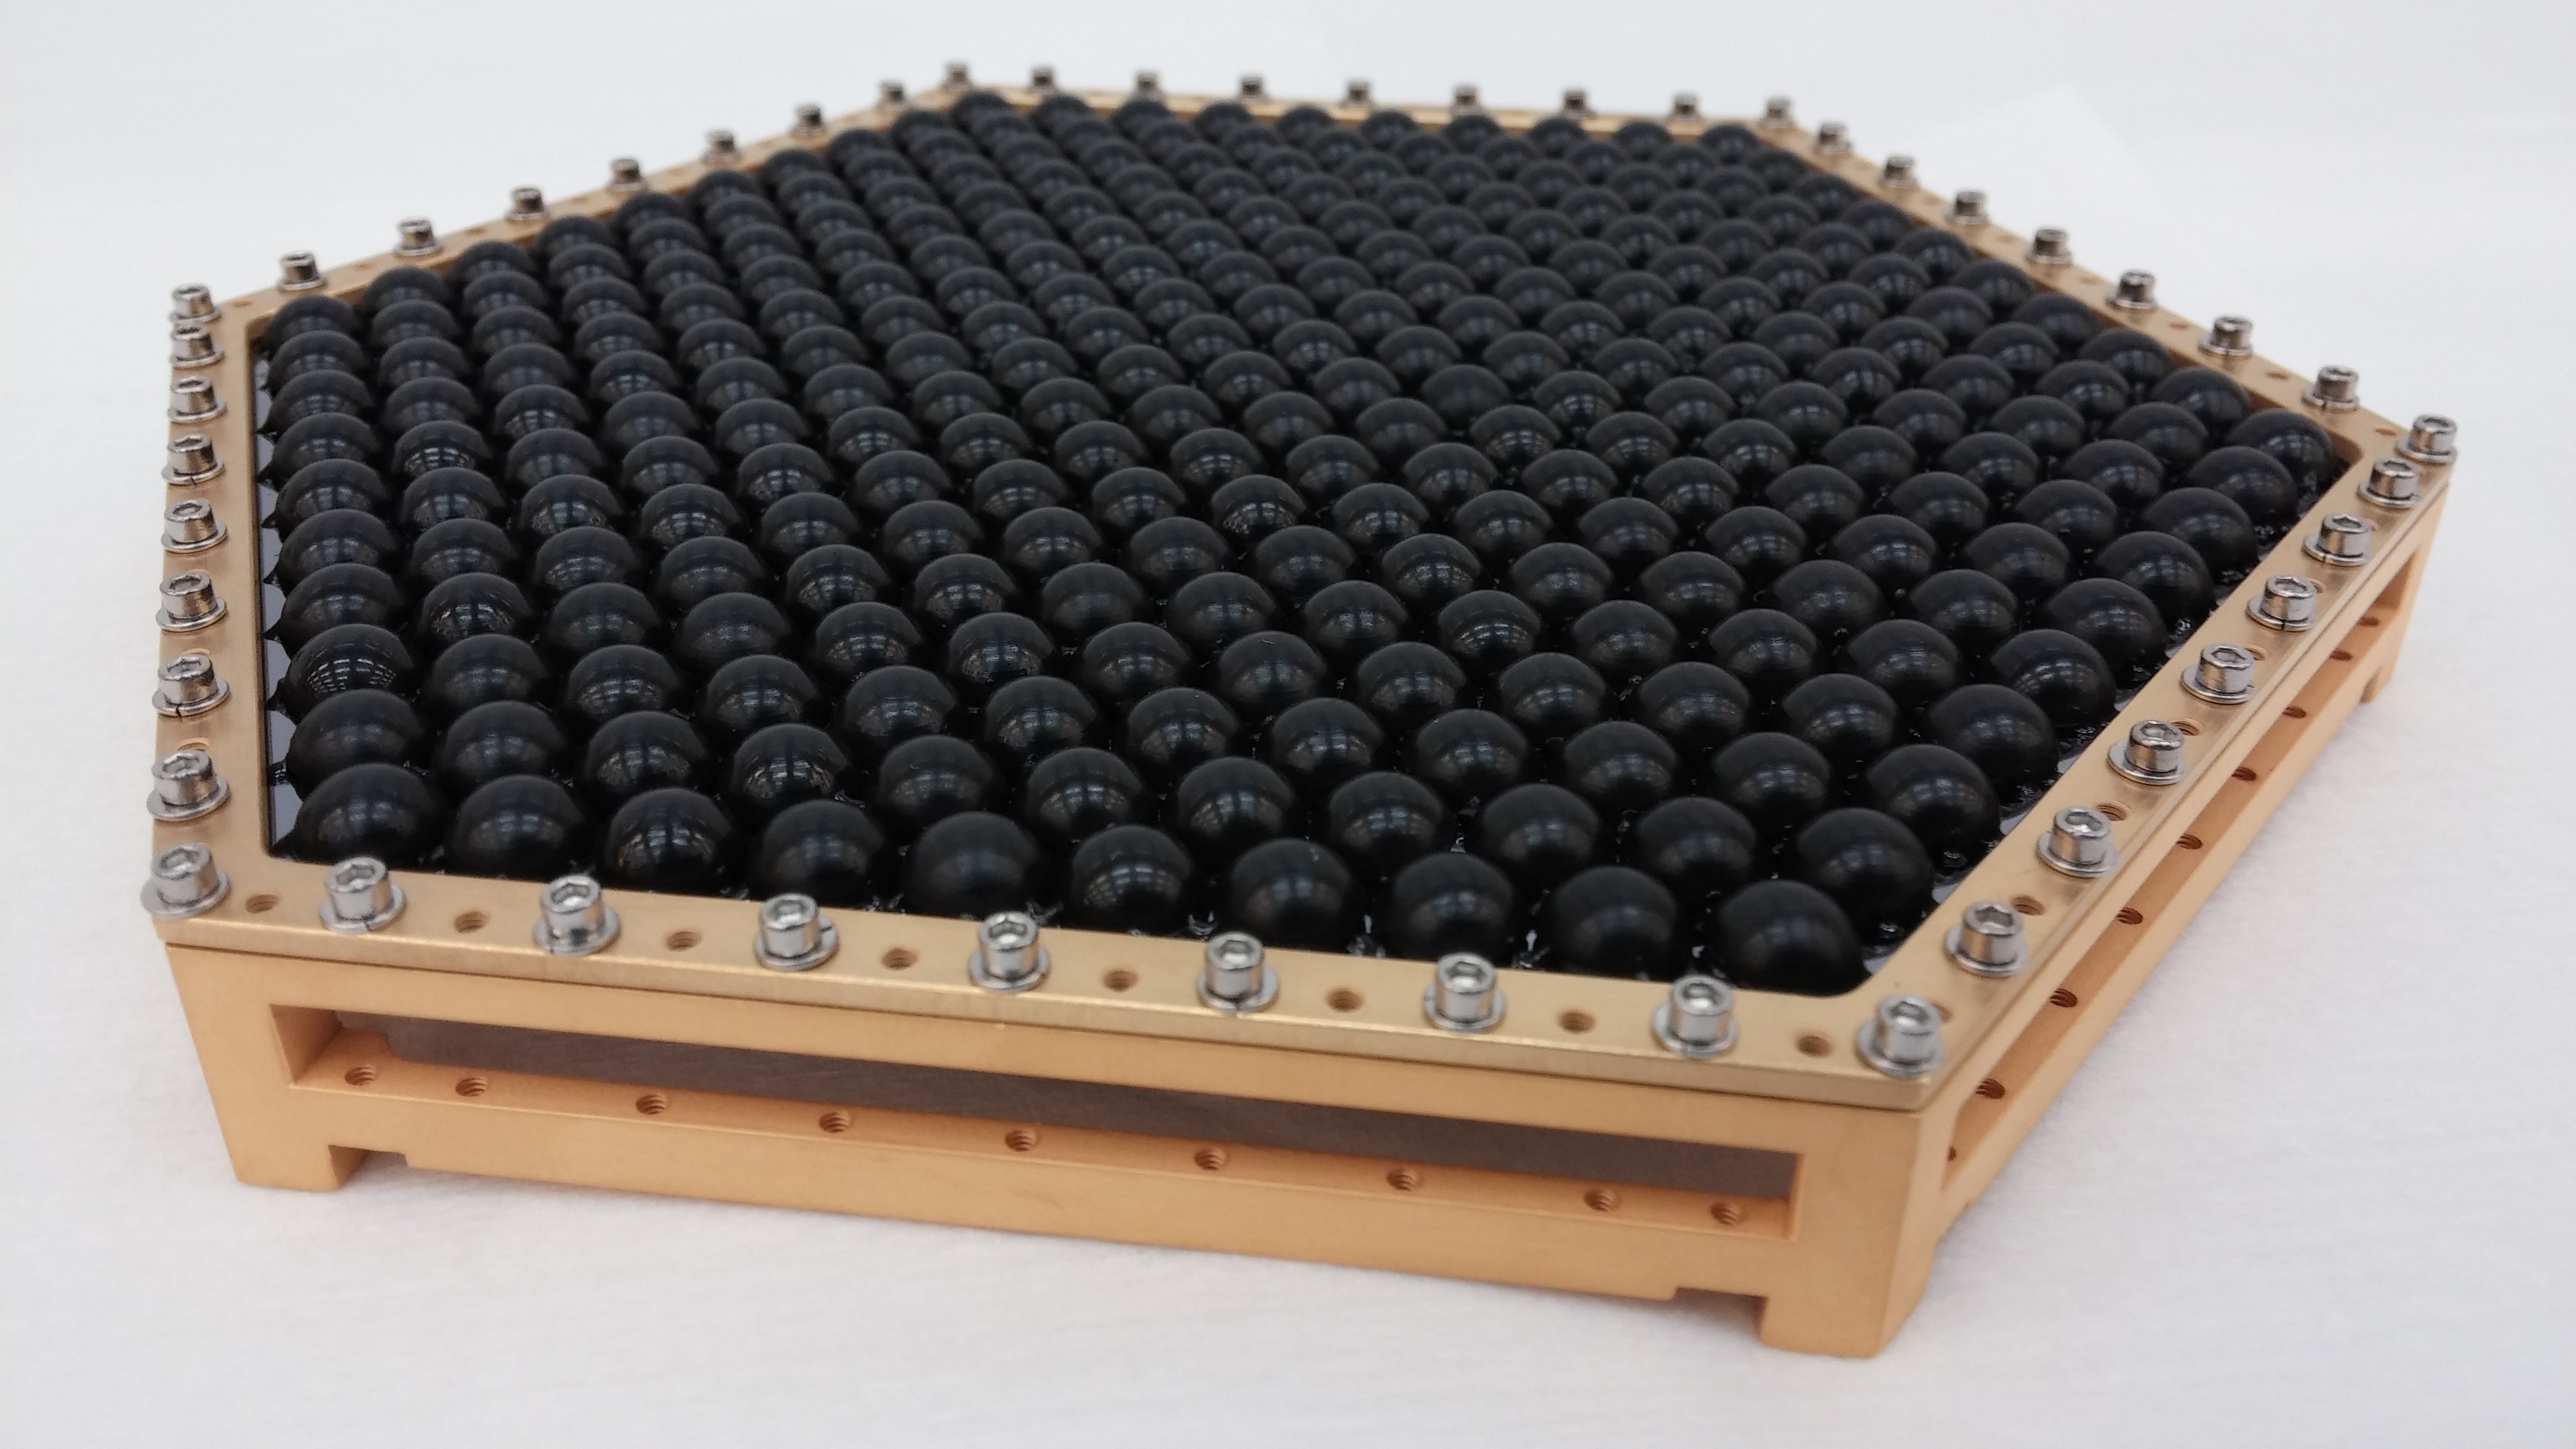
\includegraphics[width=0.48\linewidth, trim=0cm -1cm 0cm 0cm, clip]{InstrumentOverview/Figures/PB2_lenslets.jpg}}
    \hfill
    \subfloat[\label{fig:focal_plane_optics:c}]{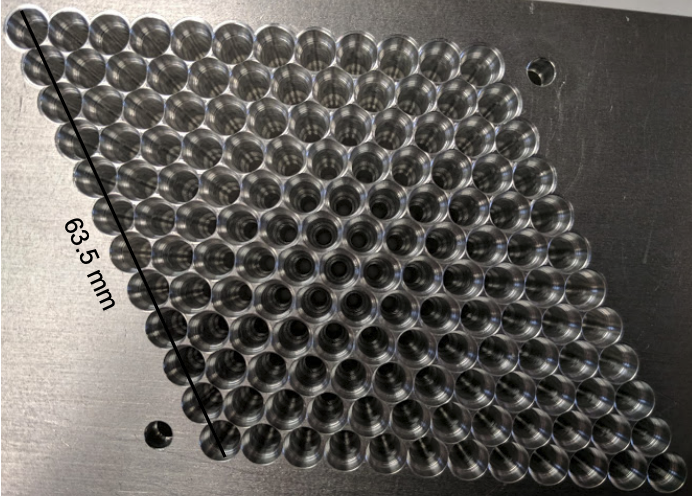
\includegraphics[width=0.48\linewidth, trim=0cm 0cm 0cm 0cm, clip]{InstrumentOverview/Figures/SO_horns.png}}
    \subfloat[\label{fig:focal_plane_optics:d}]{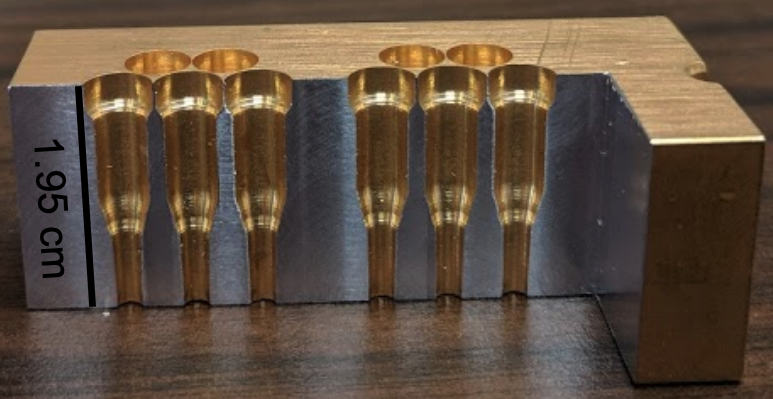
\includegraphics[width=0.48\linewidth, trim=0cm -2.9cm 0cm 0cm, clip]{InstrumentOverview/Figures/SO_horns_crossSection.png}}
    \caption[Simons Array and Simons Observatory focal plane optics]{SA and SO focal plane optics. (a) shows a PB-2a wafer, which has 271 dichroic detector pixels comprised of sinuous antennas which sense 90 and 150~GHz, and (b) shows the lenslet array that focuses light onto the antennas. In this photo, the lenslets are AR coated with two layers of Stycast, which is the lenslet technology used by PB-2a and PB-2b, but PB-2c and SO are researching alternative lenslet AR coating technologies. (c) and (d) show a prototype feedhorn array for 90/150~GHz pixels on SO. The spline profile optimizes for favorable beam properties while packing the pixels closely without optical crosstalk. Sinuous and lenselt photos courtesy of Aritoki Suzuki, and feedhorn photos courtesty of Sara Simon.}
    \label{fig:focal_plane_optics}
\end{figure}

The SA detector arrays are composed of seven \important{detector wafers}, each of which contains 271 detector pixels. The sensing element for the SA detector pixels is a planar sinuous antenna coupled to a hemispherical lenslet. The reimaging lenses focus the light onto the tip of the lenslet, which in turn re-focuses the light onto the antenna feed. The sinuous antenna is a fractal antenna whose logarithmically repeating pattern make sensitivie over a broad bandwidth. The high- and low-frequency cutoffs of the antenna are set by the minimum feature size and by the overall antenna size, respectively. After the incident radiation is collected by the antenna, a transmission line carries the light through on-chip bandpass filters, which separate the 90~and~150~GHz bands while rejecting out-of-band radiation. The band-pass-admitted radiation is then dissipated onto a thermistor whose output is amplified, digitized, and stored as raw data. To ensure efficient coupling to the sinuous antenna, the lenslets are manufactured as precise hemispheres, are offset from the sinuous antenna by a silicon spacing wafer, and are oversized to ensure adequate collimation.

The SO LF detector arrays use the same lenslet-coupled antenna technique that SA does, but its MF and UHF arrays instead employ feed horns coupled to planar, lithographed polarization-discriminating orthomode transducers. A feed horn is effectively an impedance-matched waveguide, designed to transform waves propagating in free space into wave-guide modes, which can then be routed, manipulated, and detected. Feed horns come in many different varieties, and perhaps the most common type have corrugations along its walls to prevent substrate modes that can in turn induce a side-lobe response. While corrugations are a tried and true technique to obtain a Gaussian, symmetric pixel response, they are not space efficient and therefore give rise to a substantial fraction of the focal plane area being optically inactive. To combat this issue, SO (building the work of Advanced ACT) uses smooth-walled feed horns with spline-profiled shapes to optimize over several performance metrics, including coupling to the telescope optics, cross polarization, and beam shape. Without corrugations, the array of feed horns can be very dense, with only hundreds of microns separating adjacent detector pixels. This setup in turn increases the detector count per telescope, which improves the sensitivity of the experiment.

%%%%%%%%%%%%%%%%%%%%%%%%%%%%%%%%
%%%%%%%%%%%%%%%%%%%%%%%%%%%%%%%%

\subsection{Telescope to focal plane coupling}
\label{sec:beam_coupling}

Given a high-level overview of the SA and SO pixel architectures, we now move to quantify the coupling between the focal plane and the telescope, which is central to many of the sensitivity calculations in following chapters. Assuming a diffraction-limited optical system, the magnification of the optics tube is quantified by the \important{F-number} (also sometimes called the ``focal ratio'') at the focal plane
\begin{equation}
    F = \frac{D_{\mathrm{apert}}}{f} \, ,
    \label{eq:fnumber}
\end{equation}
where $D_{\mathrm{apert}}$ is the diameter of the aperture stop (or, for the SA telescope and SO LAT, the Lyot stop) and $f$ is the focal length of the focal plane image. The F-number quantifies the magnification of the optical system: given a fixed aperture size, a larger/smaller F-number leads to a smaller/larger focal plane size or equivalently a smaller/larger magnification.

\begin{figure}
    \centering
    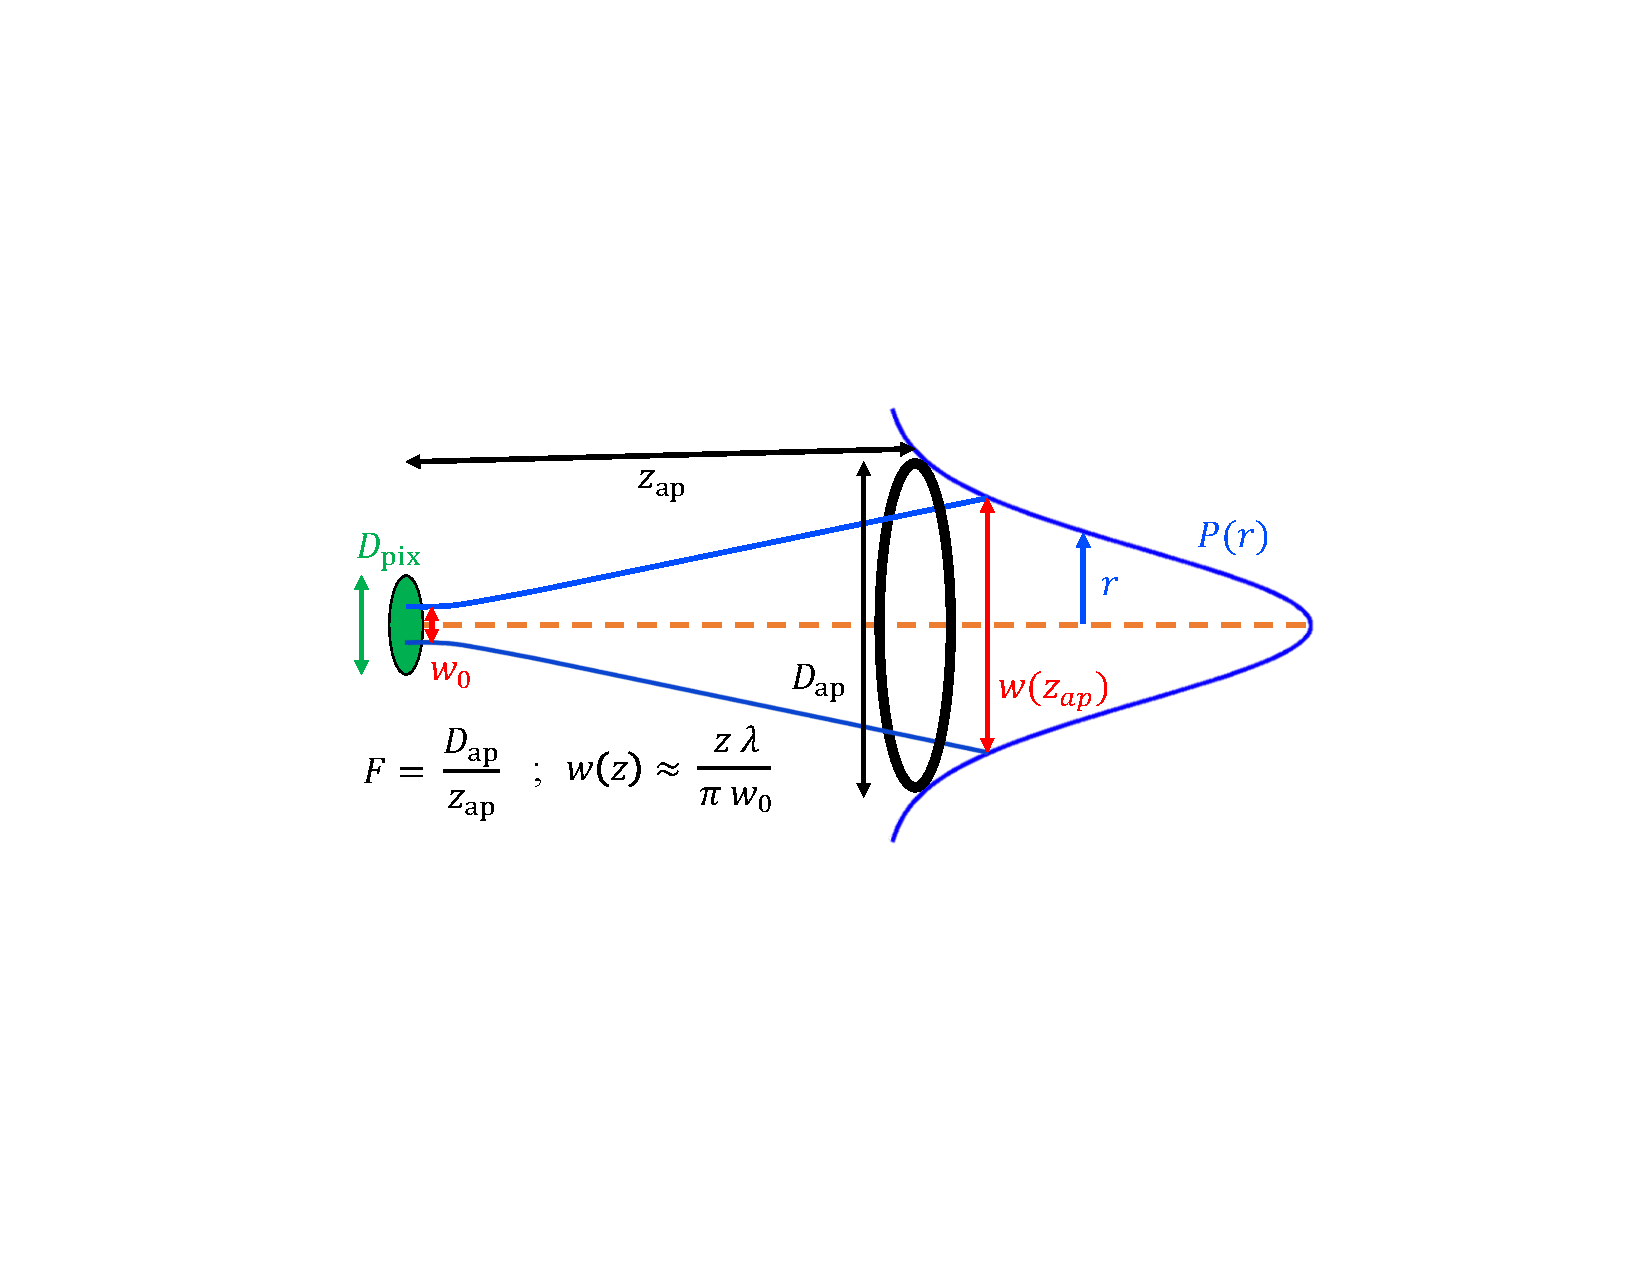
\includegraphics[width=\linewidth, trim=5cm 7cm 5cm 7cm, clip]{InstrumentOverview/Figures/beam_coupling_efficiency.pdf}
    \caption{A schematic of how the green detector pixel with diameter $D_{\mathrm{pix}}$ might illuminate the aperture stop of diameter $D_{\mathrm{ap}}$ and distance $z_{\mathrm{ap}}$ from the focal plane. The size of the beam at the aperture $w(z)$ is inversely proportional to its beam waist $w_{0}$, and the approximation applies in the \important{Rayleigh limit} where $z \gg w_{0}$.}
    \label{fig:beam_coupling_efficiency}
\end{figure}

As long as the pixels are large compared to the wavelength, they will induce minimal diffractive ringing, and therefore their \important{beam} (or equivalently, their response as a function of opening angle and/or x/y/z position) is well-approximated by a Gaussian function. In particular, detector's far-field response is given as
\begin{equation}
    B_{\mathrm{pix}}(\theta, \lambda) = \exp \left( \frac{-\theta^{2}}{2 \theta_{\mathrm{pix}}^{2}} \right) \, ,
    \label{eq:detector_pixel_beam}
\end{equation}
$\theta$ is the ray angle with respect to zenith and where
\begin{equation}
    \theta_{\mathrm{pix}} = \frac{\lambda}{\pi w_{0}} \, .
    \label{eq:pixel_beam_divergence}
\end{equation}
Here, the angular width of the pixel beam is inversely proportional to its \important{beam waist} $w_{0}$, which in turn can be related to the pixel diameter $D_{\mathrm{pix}}$ under the assumption of diffraction-limited optics
\begin{equation}
    w_{0} = \frac{D_{\mathrm{pix}}}{w_{\mathrm{f}}} \, .
\end{equation}
The most important result of this diffraction-limited formalism is that larger/smaller pixels produce a tighter/wider beam, and this in turn impacts how the detector pixel couples to the telescope.

There are two useful ways to conceptualize the relationship between the telescope and focal plane optics. The first way is to think in the forward-time sense, which is to imagine photons propagating from the sky to the detectors. In this paradigm, the image formed by the telescope becomes smaller with larger F-number (larger magnification), which in turn favors smaller pixels. The second and equally valid way is to think in the \important{reverse-time sense}, which is to imagine photons propagating form the detectors to the sky. In this paradigm, a larger F-number corresponds to a wider aperture, which in turn favors a wider pixel beam. While these two paradigms are equivalent, it will be most convenient to calculate telescope-pixel coupling efficiency from the pixel's perspective, in the reverse-time sense.

From the perspective of the detector pixel, the opening half angle of the aperture stop is
\begin{equation}
    \theta_{\mathrm{f}} = \arctan \left( \frac{1}{2 F} \right) \approx \frac{1}{2 F}\, ,
    \label{eq:stop_angle}
\end{equation}
where the approximation applies in the \important{paraxial limit}, or the small-angle regime. Given this angle, the coupling between the telescope and the detector pixel's beam is often called the \textit{beam coupling efficiency}
\begin{equation}
    \eta_{\mathrm{apert}} = \frac{\int_{0}^{{\theta_{\mathrm{f}}}} B_{\mathrm{pix}}(\theta, \lambda) \dd \theta}{\int_{0}^{{\pi / 2}} B_{\mathrm{pix}}(\theta, \lambda) \dd \theta} = 1 - \exp \left[ -\frac{\theta_{\mathrm{f}}^{2}}{2 \theta_{\mathrm{pix}}^{2}} \right] \approx 1 - \exp \left[ -\frac{1}{2} \left( \frac{\pi D_{\mathrm{pix}}}{w_{\mathrm{f}} F \lambda} \right)^{2} \right] \, ,
    \label{eq:beam_coupling_efficiency}
\end{equation}
where again the second equivalent relies on the paraxial approximation. Note that this beam-spill treatment only applies in the diffraction-limited paradigm, which has a constant throughput of $A \Omega = \lambda^{2}$. In other words, making the pixel bigger does not change the amount of light it can collect, but only the size of its far-field illumination.

\begin{figure}[!t]
    \centering
    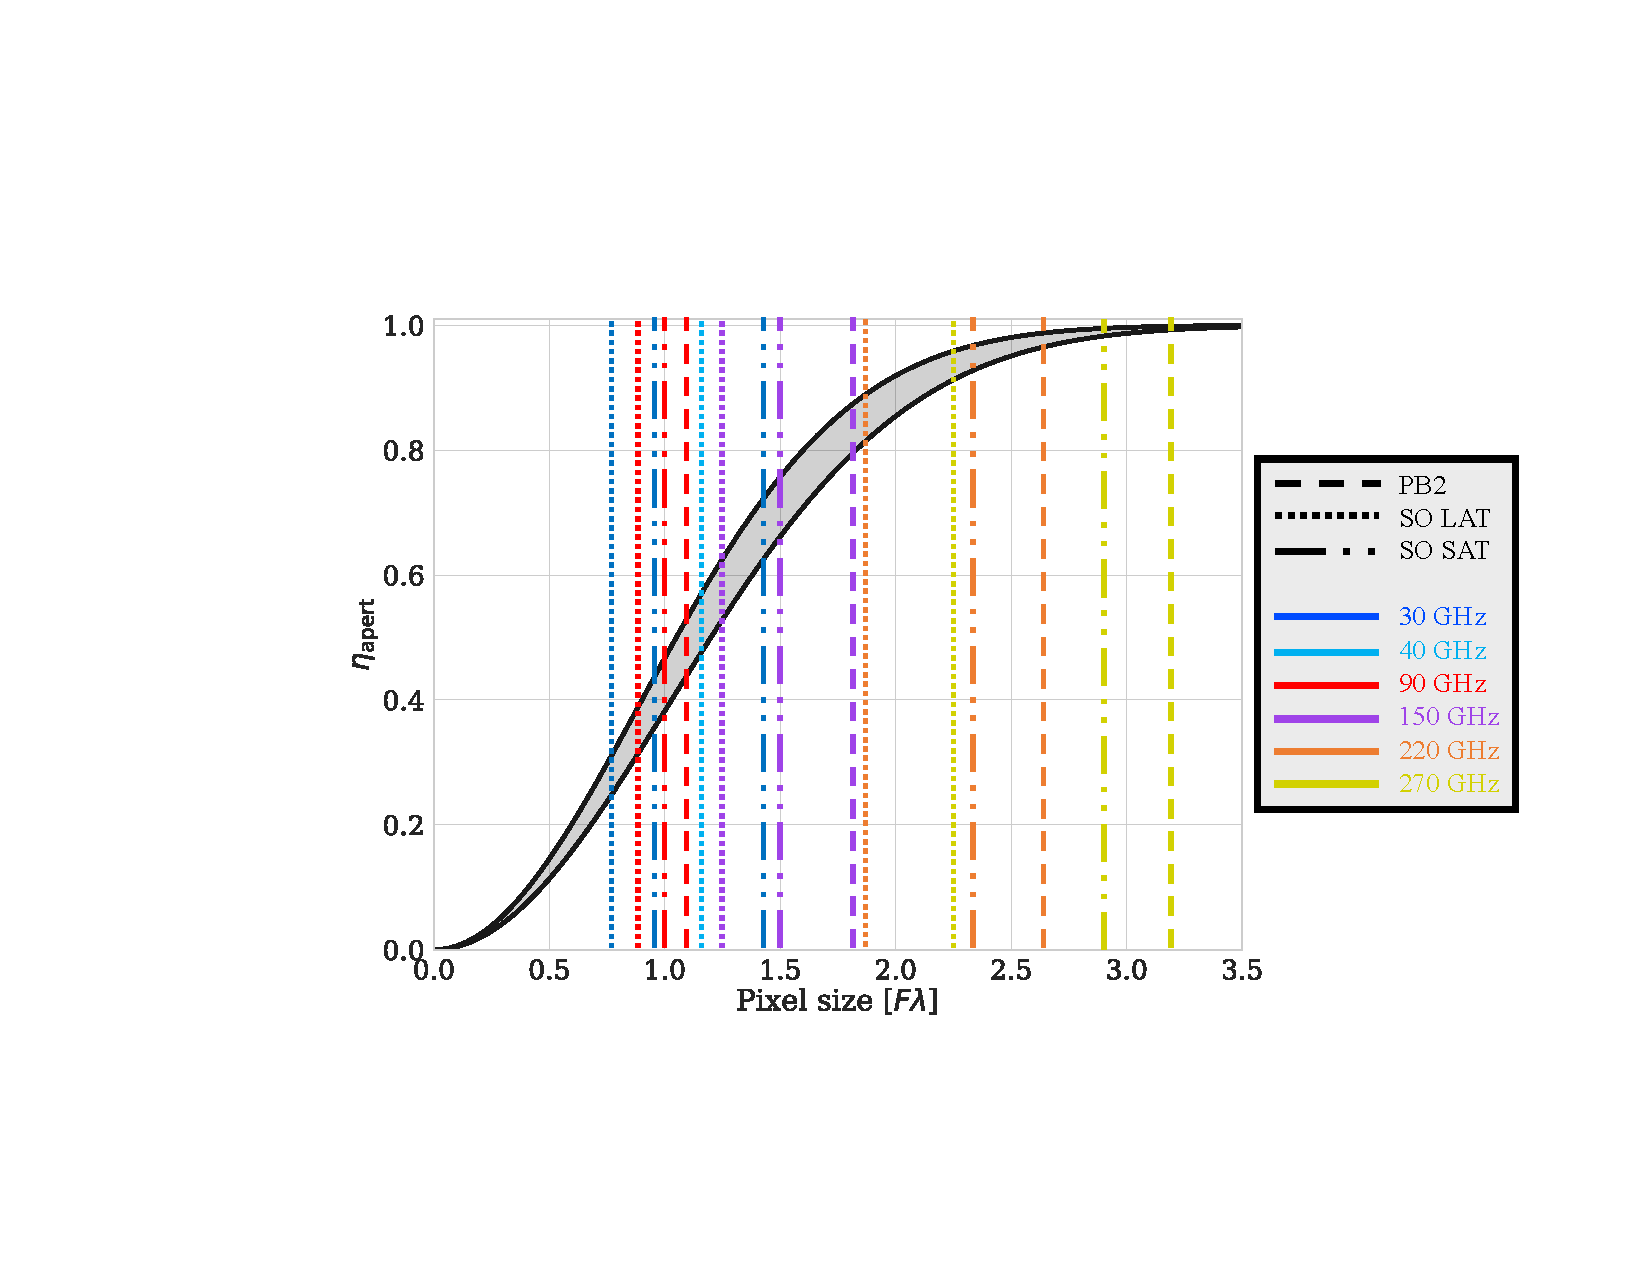
\includegraphics[width=\linewidth, trim=5cm 4cm 1cm 5cm, clip]{InstrumentOverview/Figures/aperture_eff_pix_sizes.pdf}
    \begin{tabular}{m{3.5cm}|m{3.5cm}|m{2cm}|m{3.5cm}|m{0.7cm}}
         Pixel & Coupling & $D_{\mathrm{pix}}$ [mm] & $D_{\mathrm{pix}} / F \lambda$ & $\eta_{\mathrm{spill}}$ \\
         \hline
         \hline
         SA 90/150~GHz & Lenslet + Sinuous & 6.8 & \shortstack{90~GHz: 1.1 \\ 150~GHz: 1.8} & \shortstack{0.54 \\ 0.85} \\
         \hline
         SA 220/270~GHz & Lenslet + Sinuous & 6.8 & \shortstack{220~GHz: 2.6 \\ 270~GHz: 3.2} & \shortstack{0.98 \\ 0.99} \\
         \hline
         SO LF & Lenslet + Sinuous & 18.3 & \shortstack{30~GHz LAT: 0.8 \\ 30~GHz SAT: 1.0 \\ 40~GHz LAT: 1.1 \\ 40~GHz SAT: 1.5} & \shortstack{0.25 \\ 0.37 \\ 0.48 \\ 0.65}\\
         \hline
         SO MF & Feed horn & 5.3 & \shortstack{90~GHz LAT: 0.8 \\ 90~GHz SAT: 1.0 \\ 150~GHz LAT: 1.2 \\ 150~GHz SAT: 1.5} & \shortstack{0.25 \\ 0.37 \\ 0.51 \\ 0.71} \\
         \hline
         SO UHF & Feed horn & 5.3 & \shortstack{220~GHz LAT: 1.8 \\ 220~GHz SAT: 2.3 \\ 270~GHz LAT: 2.2 \\ 270~GHz SAT: 2.9} & \shortstack{0.79 \\ 0.92 \\ 0.90 \\ 0.97} \\
         \hline
    \end{tabular}
    \caption{Beam coupling efficiencies for SA and SO detectors. The top panel shows the shows the loation of the pixel sizes in units of $F \lambda$ along the $\eta_{\mathrm{apert}}$ curve, and the shaded region represents $2.8 \geq w_{\mathrm{f}} \geq 3.2$. There is a clear clustering of pixel sizes in the area of 1.0~$F \lambda$, which is a natural optimum that we discuss in great detail in Chapter~\ref{ch:white_noise_correlations}.}
    \label{fig:beam_coupling_eff_pixel_sizes}
\end{figure}



As evidenced by the beam coupling efficiencies in Table~\ref{tab:beam_coupling_efficiencies}, the SA and SO detector pixels are substantially illuminating the stop. While this degrades per-detector sensitivity, it allows more detectors to be packed onto the focal plane, improving overall instrument performance. In this paradigm, it is critically important for the aperture stop to be as cold as possible to limit the parasitic loading on the detectors. 

%%%%%%%%%%%%%%%%%%%%%%%%%%%%%%%%
%%%%%%%%%%%%%%%%%%%%%%%%%%%%%%%%

\subsection{Anti-reflection coatings}
\label{sec:instrument_overview_ar_coatings}

SA and use alumina and silicon refracting optics, which have a large index of refraction ($n_{\mathrm{alumina}} \approx 3.1$, $n_{\mathrm{silicon}} \approx 3.4$) compared to that of vacuum $n = 1$. Therefore, without anti-reflection (AR) coatings, a bare vacuum-optic interface, will have a reflectivity of $R = [(n - 1) / (n + 1)]^{2} \sim 30$\% at normal incidence and even worse at oblique angles. Given that each lens has two surfaces and that there are three lenses per optics tube, the transmittivity of the receiver without any anti-reflection (AR) coatings would be $T = (1 - r)^{6} = 15$\%. In addition, such large reflectivities encourage multiple reflections within the cryostat that can great near-field images that can show up as \textit{ghosts} in the resulting sky image. Therefore, AR coatings play a critical role in the optical performance of the receiver. AR coatings are discussed in greater detail in Section~blah.

\begin{figure}[!t]
    \centering
    \subfloat[\label{fig:cmb_instrument_ar_coatings:a}]{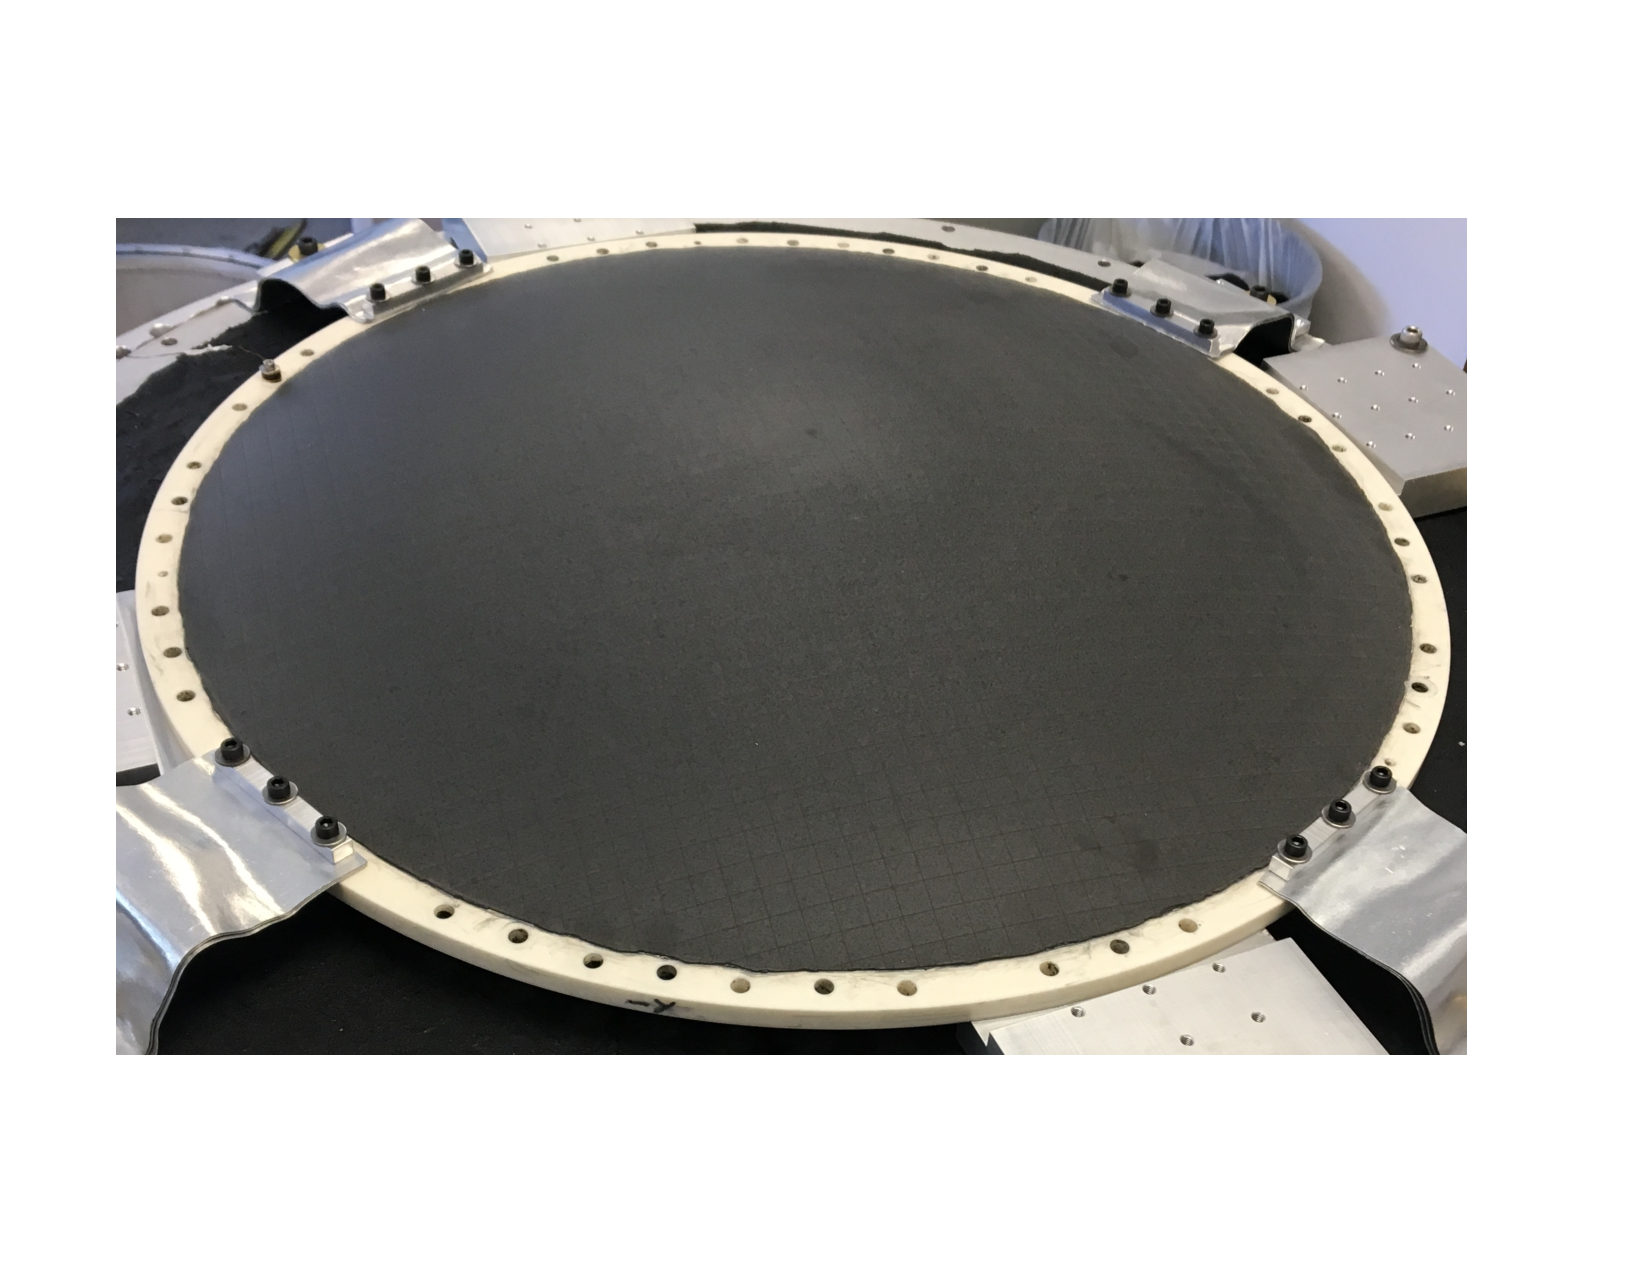
\includegraphics[width=0.48\linewidth, trim=2cm 4cm 2cm 4cm, clip]{InstrumentOverview/Figures/epoxy_ar_coating_example.pdf}}
    \subfloat[\label{fig:cmb_instrument_ar_coatings:b}]{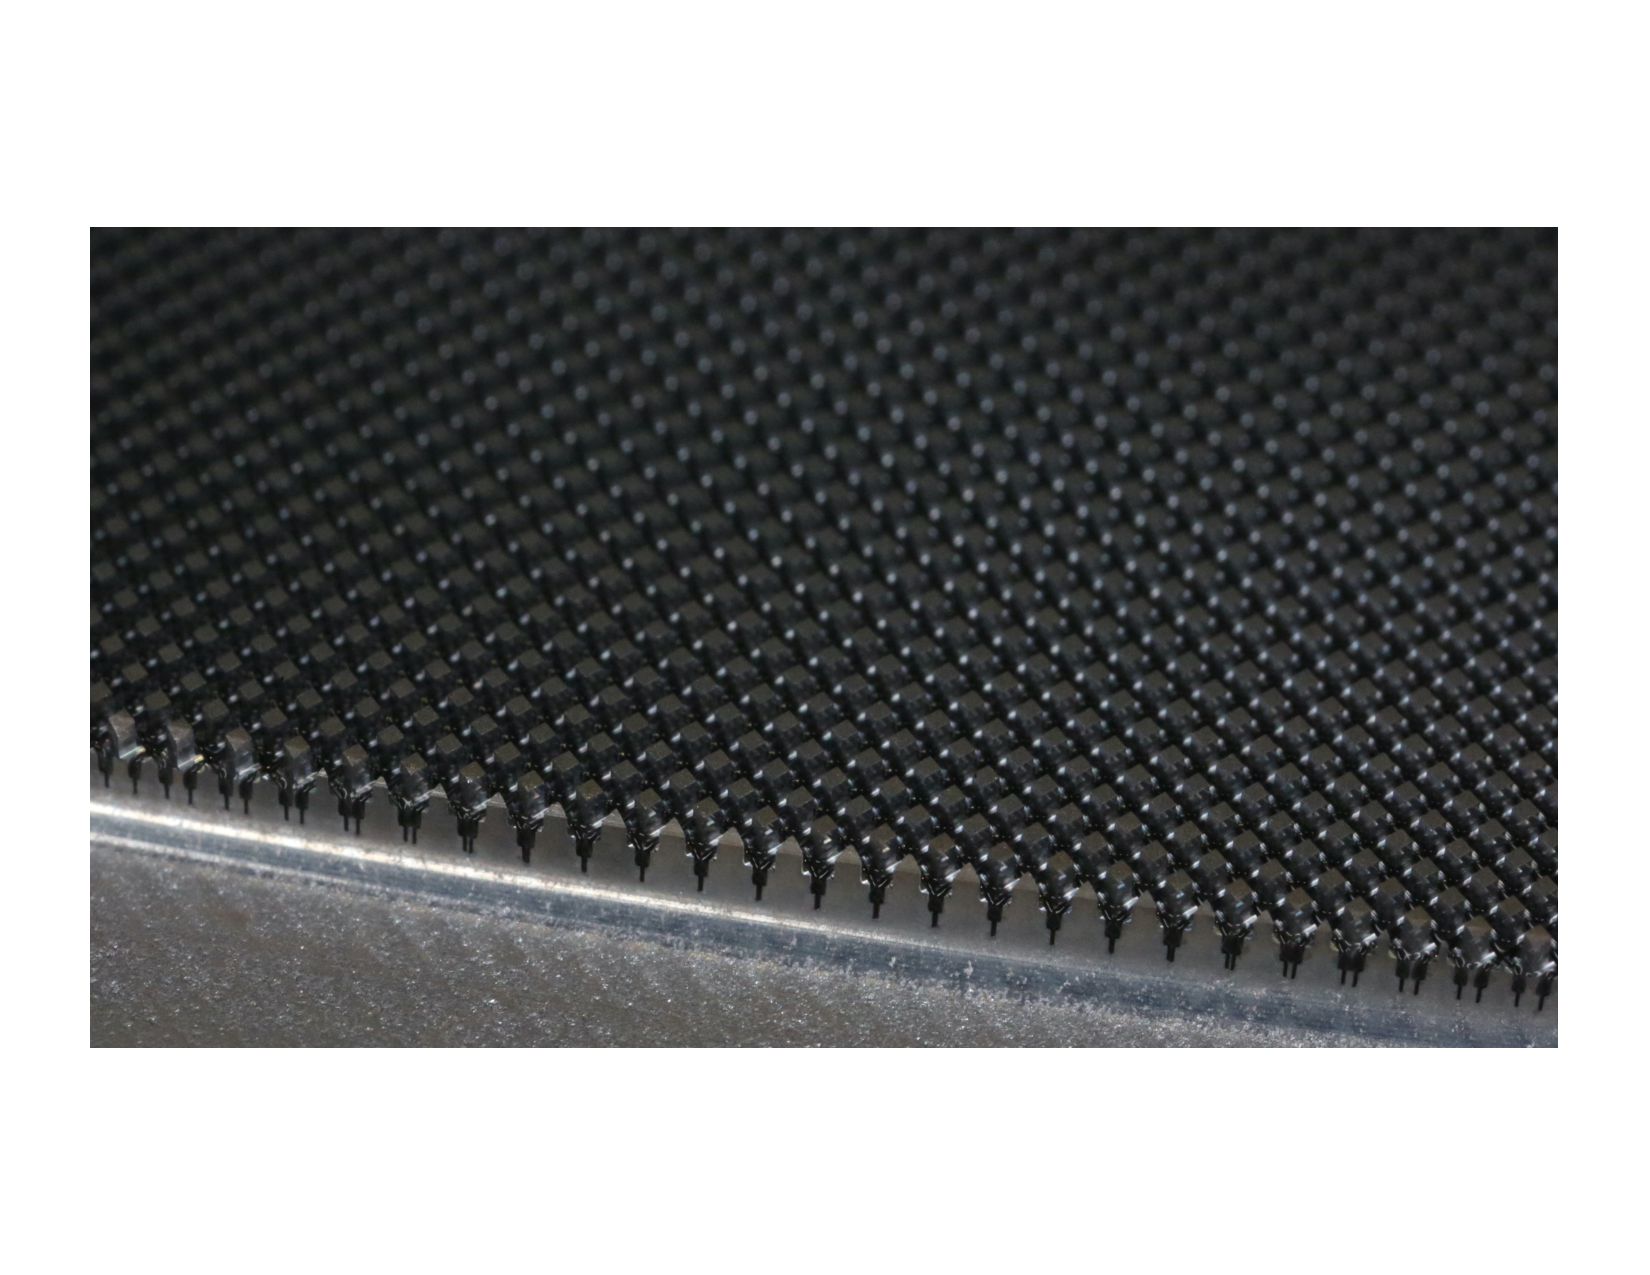
\includegraphics[width=0.48\linewidth, trim=2cm 4cm 2cm 4cm, clip]{InstrumentOverview/Figures/metamaterial_ar_coating_example.pdf}}
    \caption{AR coating technologies used within SA and SO. (a) shows the PB-2b field lens coated with two layers of epoxy mounted in a cryostat at LBNL right before thermal testing. The dicing lines are for strain relief and are cut by a UV laser, and the diameter of the part is 500~mm. (b) shows an SO MF silicon lens with three layers of metamaterial AR. The pitch between ``pillars'' is 0.4~mm. The silicon photo is courtesy of Joey Golec.}
    \label{fig:cmb_instrument_ar_coatings}
\end{figure}

SA's alumina/silicon AR coatings are composed of several technologies that have matured during the course of the project. All coatings are dicrhoic and comprise two distinct layers with optimal index and optimal thickness. In PB-2a, the curved sides of the lenses are coated with two layers of Stycast epoxy, which is molded onto the surface during the epoxy cure and milled to thickness after the mold is removed. The flat sides of the lenses are coated with a bottom layer of plasma-sprayed Mullite and a top layer of an expanded polyimide foam glued using melted low-density polyethylene. The former technology was developed at Berkeley in California, while the latter was developed at the KEK high-energy laboratory in Japan. PB-2 and PB-2c, on the other hand use plasma-sprayed alumina loaded with various fillers to adjust the layer's index. The layers are applied directly onto the lens surface with a finely tuned thickness, and the density is controlled via tuning of plasma-spay parameters, which in turn controls the layer density. Each of these technologies have their own advantages and disadvantages, but all of them attain a reflectivity of $\sim$~1\%, amounting to a total lens throughput of $\sim$~90\%. Given the huge importance of AR coatings in the receiver, the UC Berkeley group invests substantial resources into the development of higher-throughput, scalable, cost-effective AR coatings both for SA and for future experiments. This has led to substantial advancements in the technology, which we discuss in further detail in Section~blah.

SO's on the other hand uses \important{metamaterial} AR coatings for their alumina and silicon optics. This technique involves cutting sub-wavelength structures into the optic's surface whose geometry allows silicon/alumina and vacuum to combine to give an effective dielectric constant. This method has several advantages over the more ``traditional'' approach of adding materials to the surface. First, there are no concerns about cryogenic delamination, because there is no CTE mismatch between AR materials and the base lens materials. Second, the dielectric constant is (in theory) fully tunable via simply adjusting the sub-wavelength structure geometry. This tuning mechanism is in contrast to using plastics or epoxies, for example, which require a precise material composition to achieve the desired index that is often not easily tuned. Third, there is a smaller penalty for adding more layers, which is also driven by the lack of CTE mismatch issues. Therefore SO cuts three AR layers for their two-color instruments, which provides $\sim$~0.1\% in-band reflection, as opposed to two-layer coating which only achieves $\sim$~1\%. Not until recently have metamaterials on alumina been demonstrated, and therefore SO will be the first experiment to field sub-wavelength structures on ceramics.

%%%%%%%%%%%%%%%%%%%%%%%%%%%%%%%%
%%%%%%%%%%%%%%%%%%%%%%%%%%%%%%%%
%%%%%%%%%%%%%%%%%%%%%%%%%%%%%%%%

\section{Thermal Design}
\label{sec:optics_thermal_design}

In addition to providing a high-fidelity image of the sky onto the focal plane, the receiver the receiver optics need to reject huge amounts of infrared (IR) radiation in order to cool the detectors to sub-Kelvin temperatures. While the details of the SA and SO thermal filtering schemes differ in several ways, in this section we focus our discussion on that of SA, which will highlight the key principles of IR rejection while providing the necessary background information for SA thremal discussions in following chapters. 

As noted, the SA receiver has a 0.5~m diameter window and that the ambient temperature at the site is, on average, $\approx$~273~K, the radiative load on the cryostat is $\sim$~300~W. The sub-K refrigerator at a 0.3~K base temperature, on the other hand, has only $\sim$~5~$\mathrm{\mu W}$ of cooling power. Therefore, the receiver \important{optical stack}, which consists of not only its lenses but also several thermal filters, must reject power at one part $\sim 10^{8}$ while also being transparent to CMB photons at $\sim$~100~GHz.

\begin{figure}[!t]
    \centering
    \subfloat[\label{fig:pb2_filters:a}]{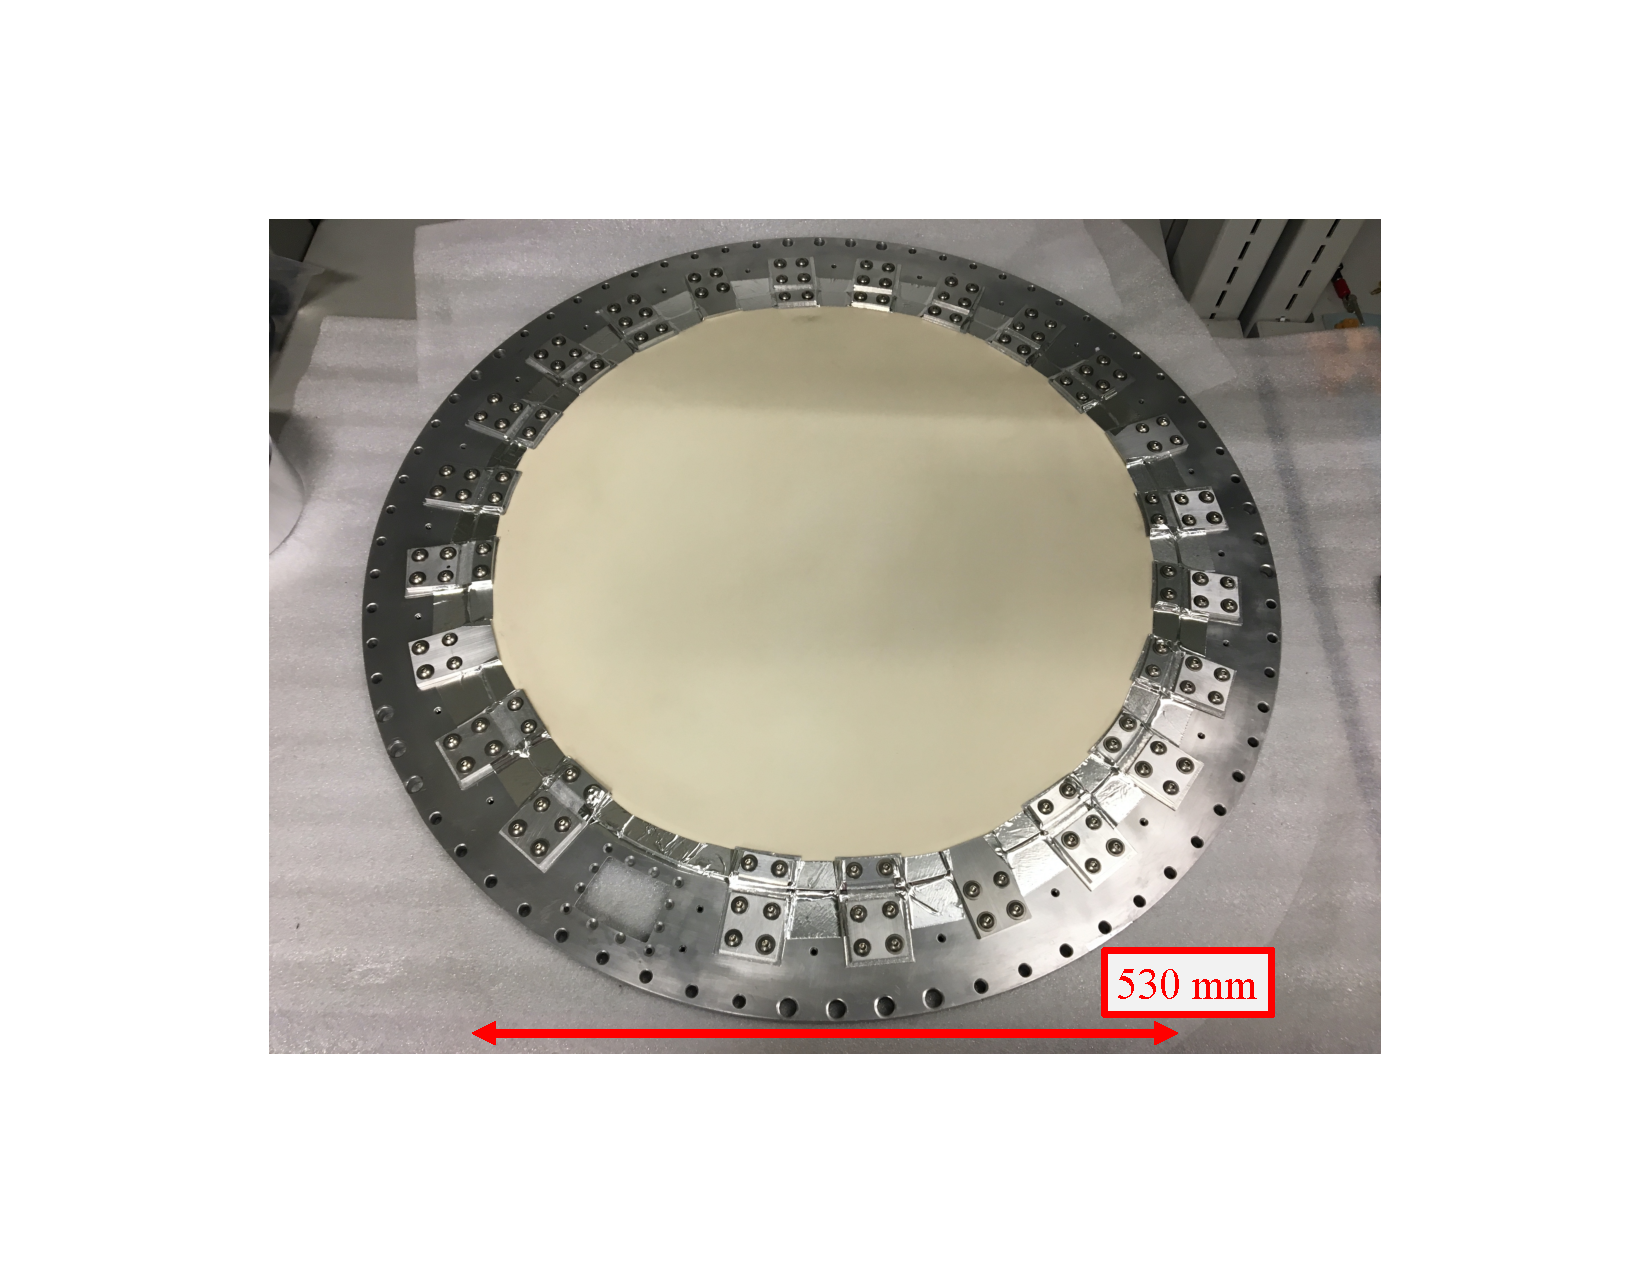
\includegraphics[width=0.48\linewidth, trim=5.5cm 3.5cm 5.5cm 3.5cm, clip]{InstrumentOverview/Figures/IRF_photo.pdf}}
    \subfloat[\label{fig:pb2_filters:b}]{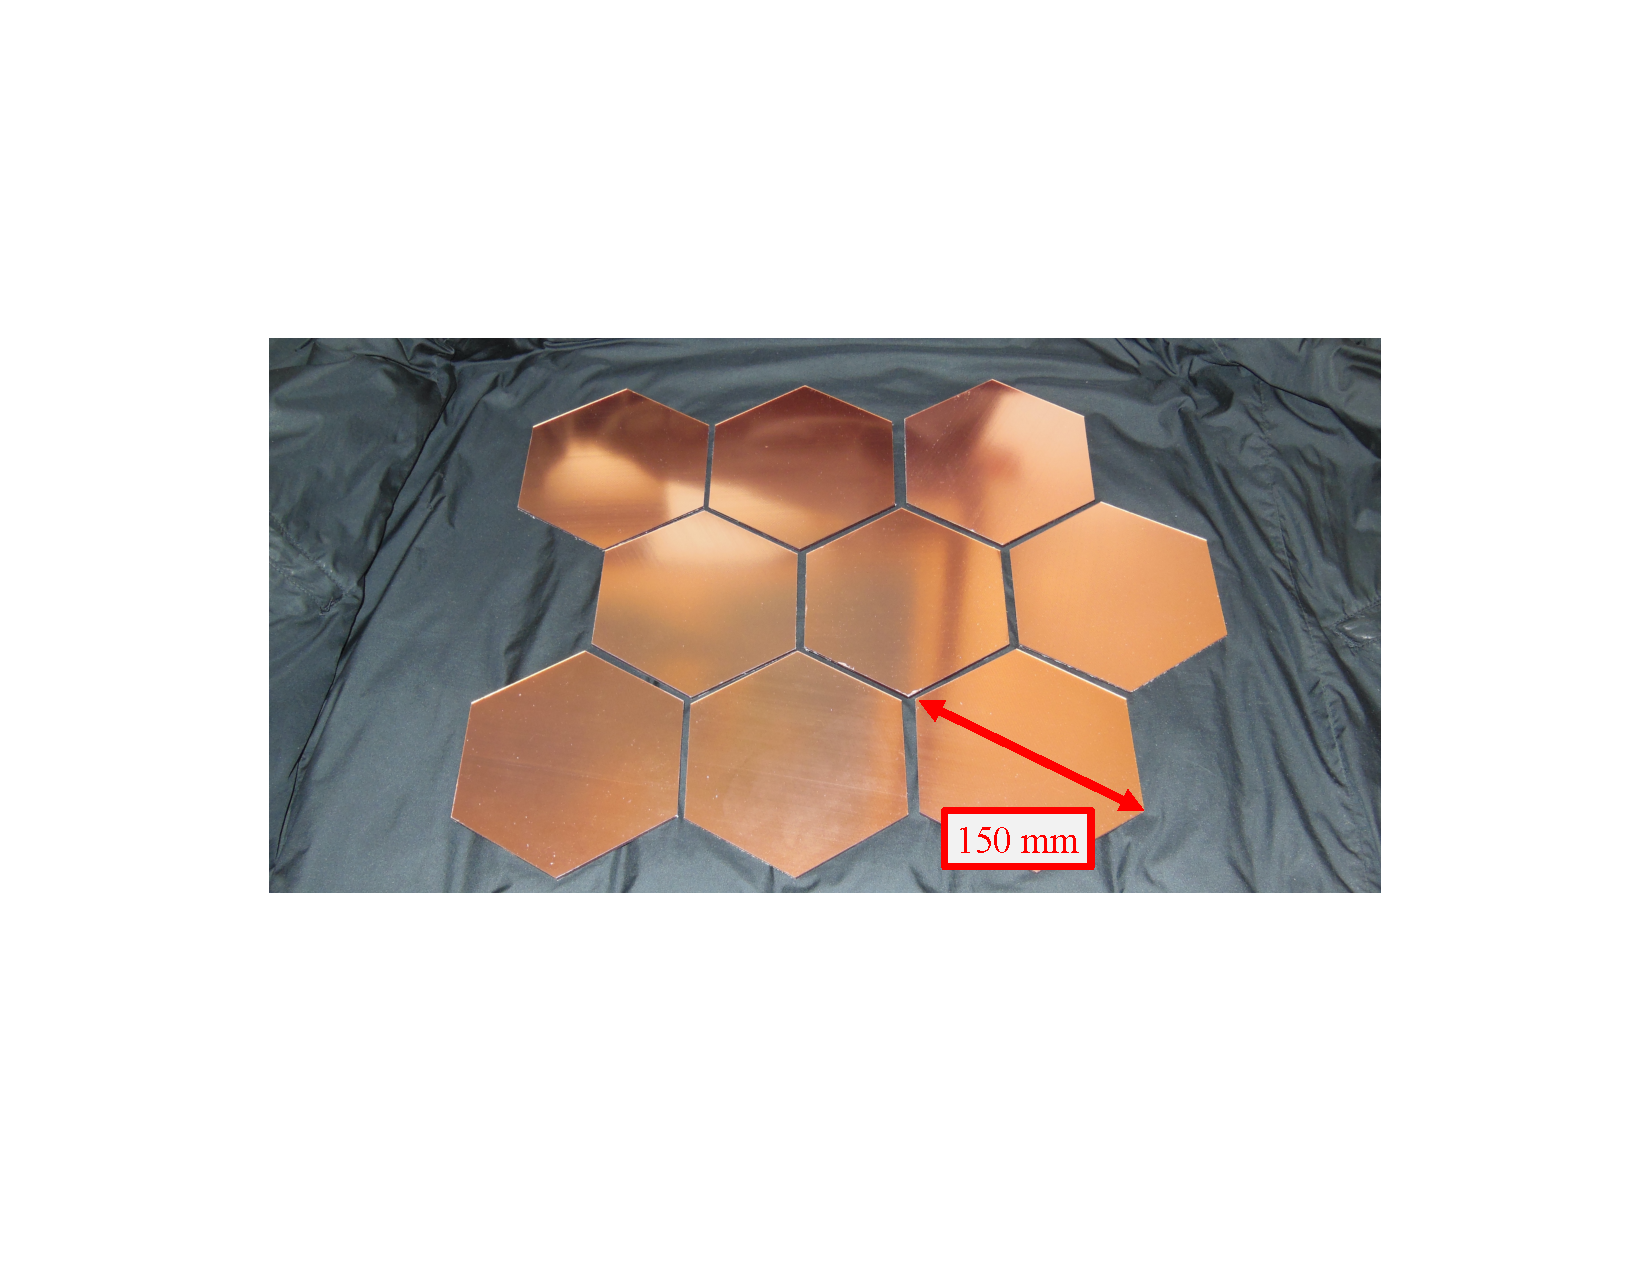
\includegraphics[width=0.48\linewidth, trim=7.2cm 5cm 7cm 5cm, clip]{InstrumentOverview/Figures/MMF_photo.pdf}}
    \caption{Caption}
    \label{fig:pb2_filters}
\end{figure}

The receiver cryostat consists of three stages, which are shown in Figure~\ref{fig:pb2_telescope}: the 50~K stage, 4~K stage, and mK stage. The 50 and 4~K stages are cooled by two Cryomech PT-415 pulse-tube refrigerators (PTRs), one of which is connected to the optics tube near the field lens, and the other of which is connected to the \important{backend} (BE). This dual-cooler system distributes the cryogenic load, dumping most of the radiative power on the OT PTR and most of the wiring-induced conductive load onto the BE PTR. Each PTR has two stages, one of which sinks $\sim$~tens of watts on the 50~K stage and another that sinks $\sim$~1~W on the 4~K stage. Given this configuration, the cryostat is built as a Russian doll of concentric shells from 300~K (the vacuum shell) to 4~K, each mounted with hollow G10 tubes, which have a low thermal conductivity, and covered with \important{multi-layer insulation} (MLI) to limit radiative loads. The mK stage is cooled by a \important{Helium-3 refrigerator}, which leverages the low boiling point of the $\mathrm{He_{3}}$ isotope to cool the focal plane to $\approx$~0.3~K. The cooling power of the mK fridge is only $\sim$~5~$\mathrm{\mu W}$, and because entropic transfer is obtained by boiling $\mathrm{He_{3}}$, the fridge must be recharged every day or two and therefore has a sub-unity duty cycle. 

In order to both keep the focal plane cold, the SA optics include a combination of absorptive and reflective IR filters. The absorptive filters are made of alumina and include a 2~mm thick flat piece at 50~K as well as the lenses at 4~K, which in addition to being refractors are good IR absorbers. These alumina optics are designed to absorb radiation $\gtrsim$~1~THz and are mounted to have high thermal conductivity to the 4~K stage, which is in turn tightly coupled to the PTC. In addition, alumina has a high thermal conductivity, which is important for keeping the optics close to isothermal and hence avoid radial thermal gradients between the optic's center (where most of the IR power propagates) and its edge (where it is thermally sunk). The reflective filters are developed at Cardiff University and are a metamaterial-layer, capacitive grid that act as low-pass reflectors.

The effectiveness of the absorptive filters relies on their conductivity to their respective cryogenic stage, and therefore much attention is payed to how the alumina optics are mounted. This strapping task is made even more challenging by the differential coefficient of thermal expansion (CTE) between the aluminum cryogenic stage and the alumina IR filter. Alumina has a CTE of $\approx$~5~ppm/C, while alumina has a CTE of $\approx$~30~ppm/C, and therefore we cannot clamp the alumina optics directly to the alumina stage without risking fracturing the alumina.

While the SO design shares many of the same principles as that of SA, there are a few key differences that ought to be highlighted. First, SO uses silicon lenses with metamaterial AR coatings. Silicon's IR absorptivity is generally lower than that of alumina and depends strongly on its resistivity, which in turn changes with temperature. Given these constraints, the SO design relies less on the lenses and more on additional filters to reject IR radiation. Second, the SO focal planes are cooled by dilution refrigerators (DRs), which operate continuously (unity duty cycle) and provide $\sim$~100~$\mathrm{\mu W}$ of cooling power at $\approx$~0.1~K. In addition, the dilution fridge has a 1~K stage with $\sim$~10~mW of cooling power, which is used to cool the LAT Lyot stop and the SAT aperture stop, as well as the lenses. Because of the DR, the SO lenses are generally cooler than those of SA, the detector operating temperatures are lower, the observation efficiency is higher, and cooling margin on the mK stage is larger.

%%%%%%%%%%%%%%%%%%%%%%%%%%%%%%%%
%%%%%%%%%%%%%%%%%%%%%%%%%%%%%%%%
%%%%%%%%%%%%%%%%%%%%%%%%%%%%%%%%

\section{Detectors}
\label{sec:simons_array_detectors}

As discussed in Section~\ref{sec:simons_array_optics}, the telescope optics couple to the detectors through an optical coupling element (either a lenslet-coupled sinuous antenna or a feed-horn-coupled OMT) via impedance-matched transmisson lines mated to on-chip bandpass filters. At this point, the filtered radiation finally reaches a \important{transition-edge sensor bolometer} (TES), which SA and SO use to detect changes in sky power. 

%%%%%%%%%%%%%%%%%%%%%%%%%%%%%%%%
%%%%%%%%%%%%%%%%%%%%%%%%%%%%%%%%

\subsection{TES operation}
\label{sec:tes_operation}

\begin{figure}[!t]
    \centering
    \subfloat[\label{fig:bolometer_operation:a}]{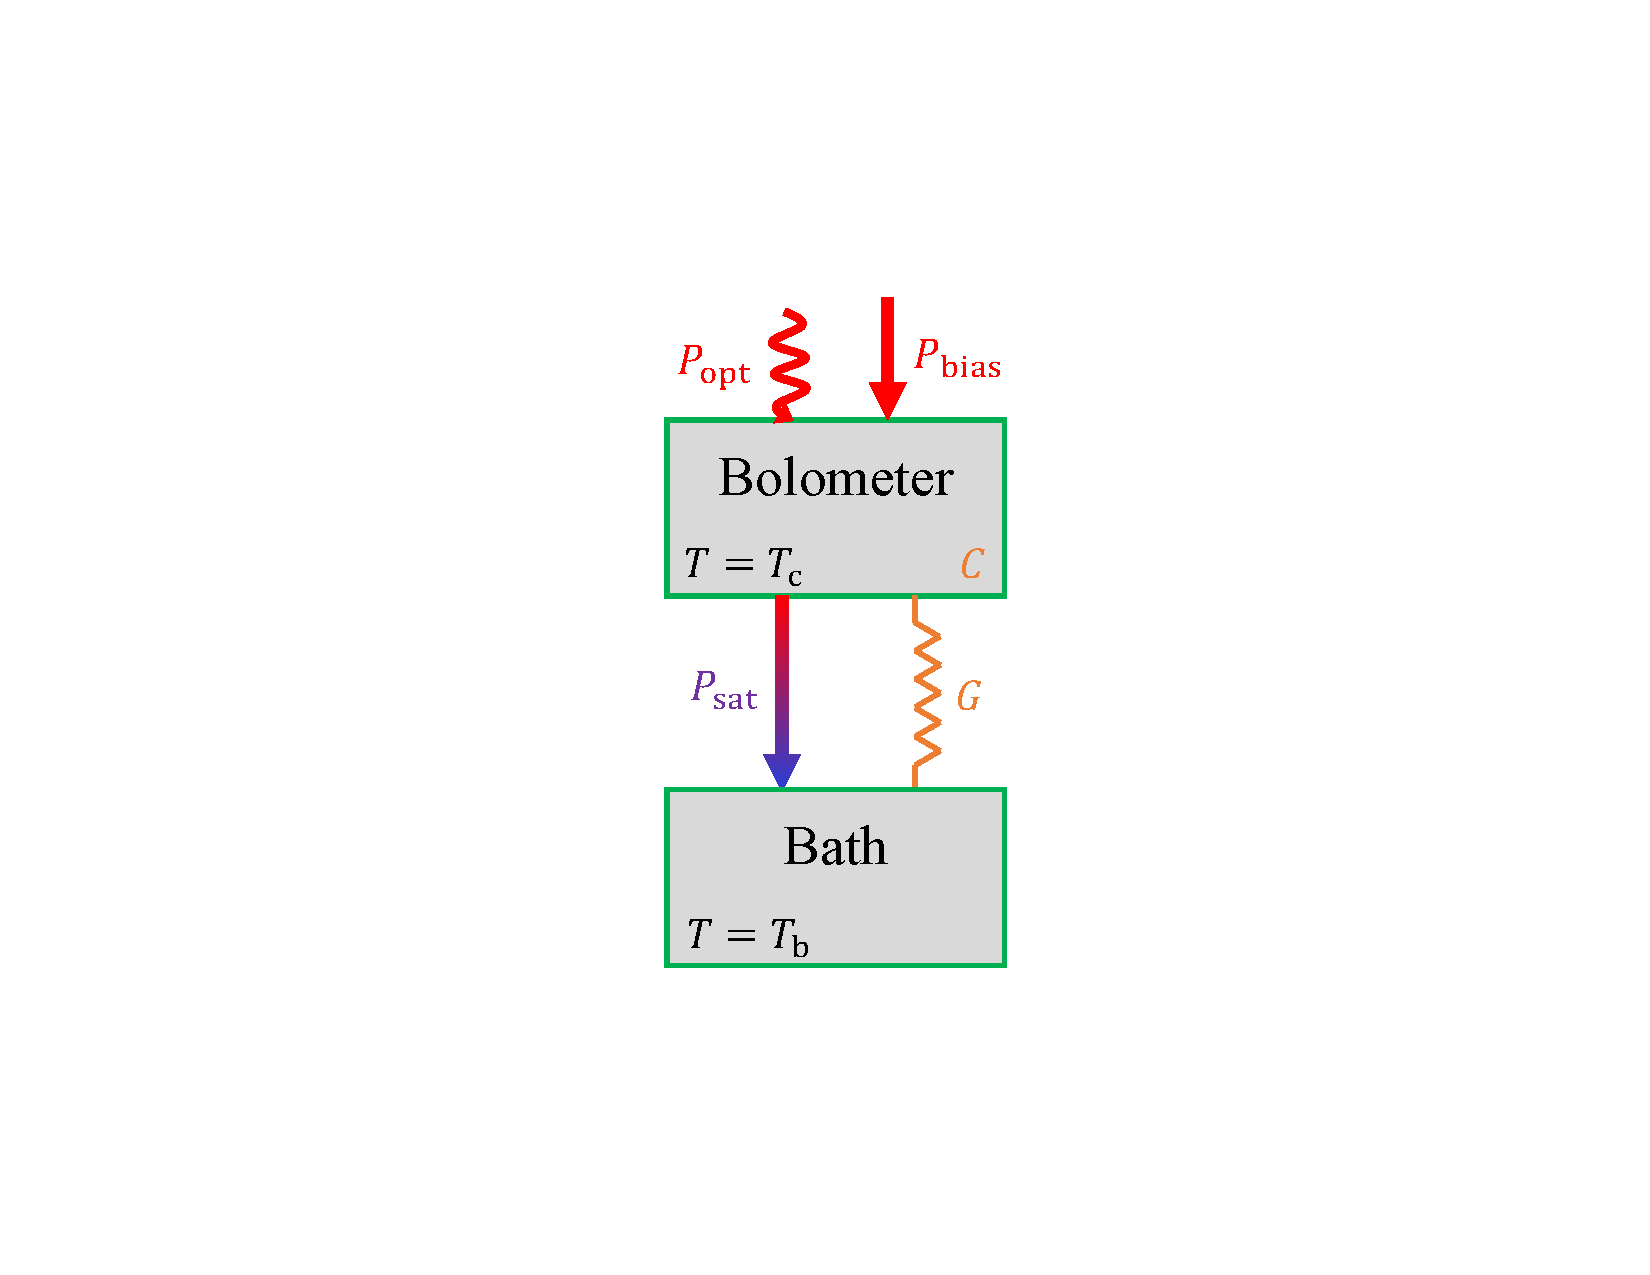
\includegraphics[width=0.35\linewidth, trim=10cm 3.5cm 10cm 5cm, clip]{InstrumentOverview/Figures/bolometer_operation.pdf}}
    \subfloat[\label{fig:bolometer_operation:b}]{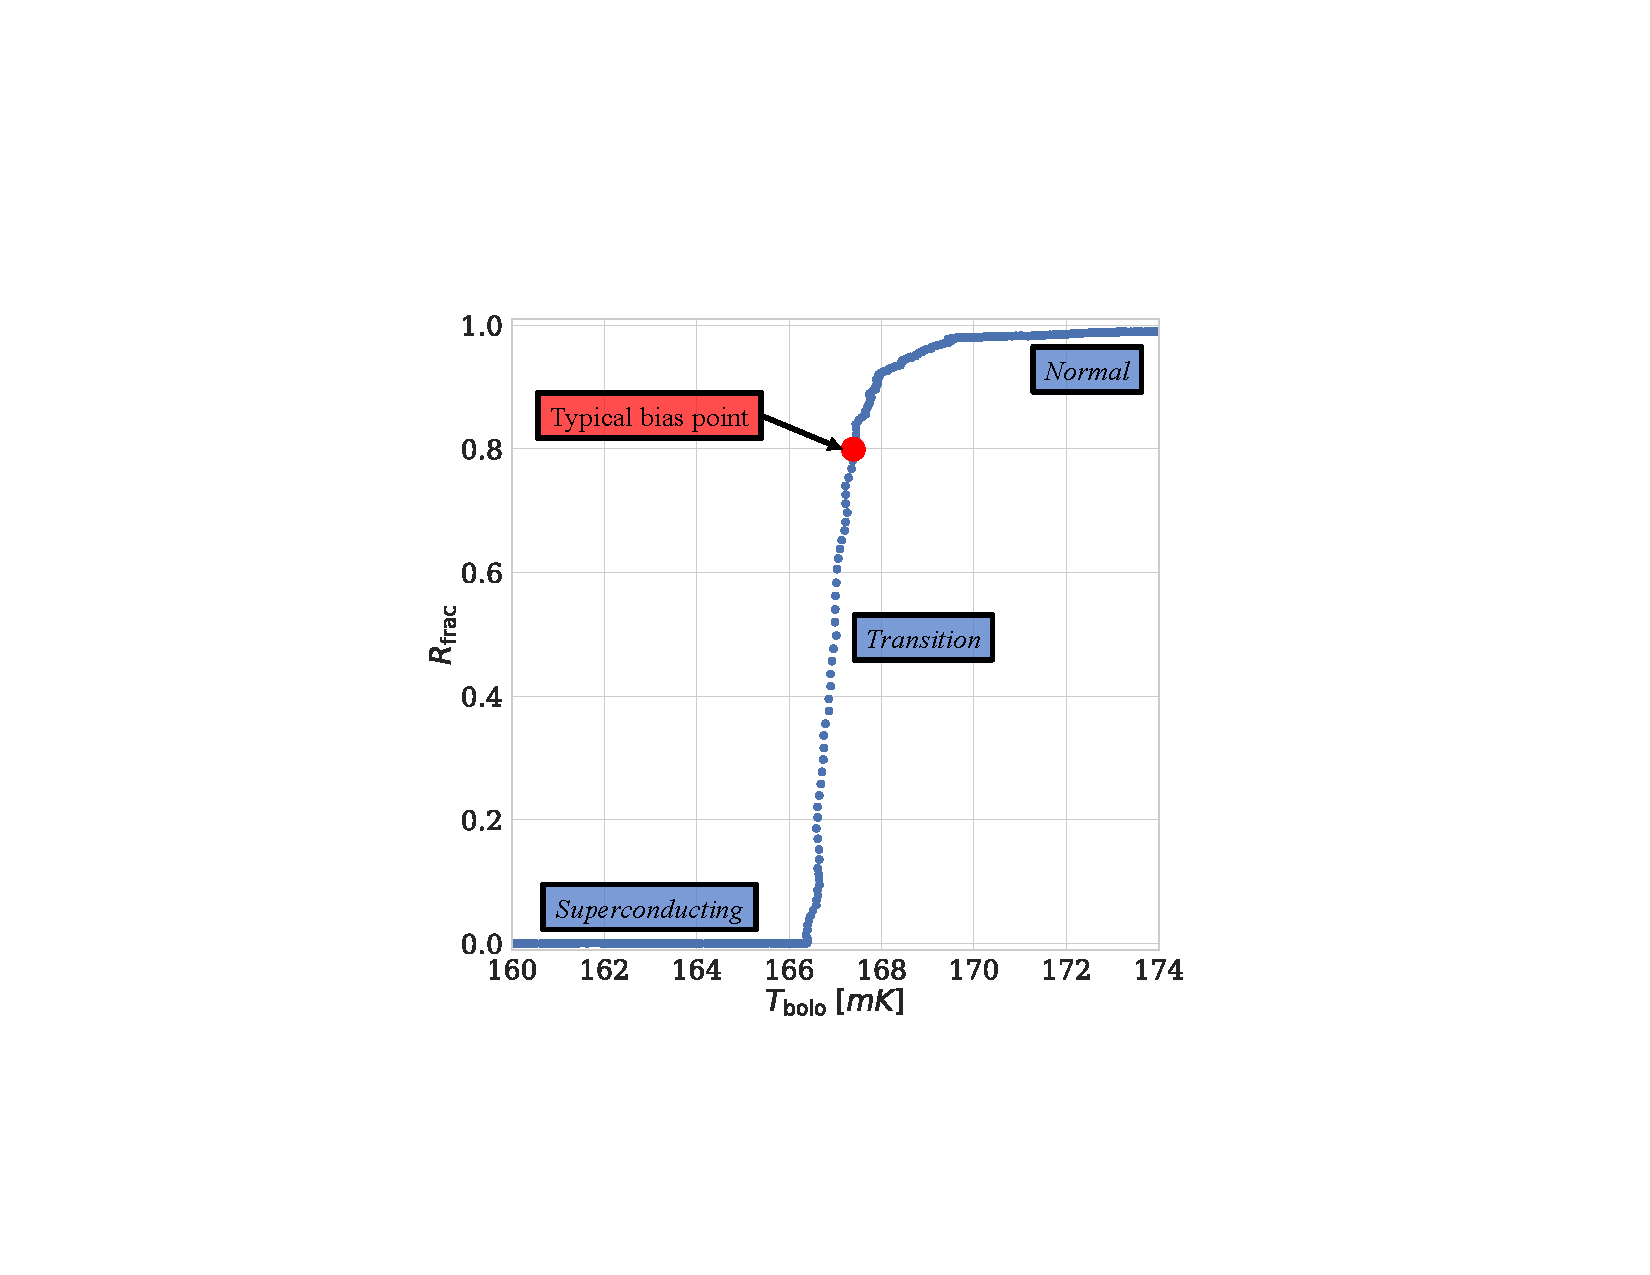
\includegraphics[width=0.63\linewidth, trim=7cm 4cm 7.5cm 5cm, clip]{InstrumentOverview/Figures/bolometer_transition.pdf}}
    \caption[Description of bolometer operation]{(a) A schematic of bolometer operation along side transition data from a TES detector for SO. The bolometer thermal element is held at its superconducting transition temperature in the presence of an optical load and an electrical (bias) load, which is balanced by a tuned thermal conduction to a thermal bath. The bias point is chosen such that, in the presence of an optical power fluctuation, $\mathrm{d}R / \mathrm{d}P_{\mathrm{opt}}$---and therefore $S = \mathrm{d}I / \mathrm{d}P_{\mathrm{opt}}$, which is called the detector responsivity---is large. In the plot on the right-hand side, the bias point is chosen to be 0.8 $\Omega$, which is approximately half of the bolometer's normal resistance.}
    \label{fig:bolometer_operation}
\end{figure}

Figure~\ref{fig:bolo_operation} shows a schematic for how the TES operates. A superconducting film is voltage biased such that the average electrical power on the bolometer is
\begin{equation}
    P_{\mathrm{bias}} = \frac{V_{\mathrm{bias}}^{2}}{R_{\mathrm{bolo}}} \, ,
    \label{eq:bolometer_p_bias}
\end{equation}
such that the total power on the bolometer is the sum of the bias power and the sky power $P_{\mathrm{opt}}$
\begin{equation}
    P_{\mathrm{tot}} = P_{\mathrm{elec}} + P_{\mathrm{opt}} \, .
    \label{eq:bolometer_power_equilibrium}
\end{equation}
The power that the TES is capable of dissipating is governed by a connection to a thermal bath with temperature $T_{\mathrm{b}}$ via a thermal link with conductivity $G$
\begin{equation}
    P_{\mathrm{sat}} = G (T_{\mathrm{c}} - T_{\mathrm{b}}) \, .
    \label{eq:saturation_power}
\end{equation}
This \important{saturation power} dictates both how much power the bolometer can absorb before saturating and how much power is due to electrical bias vs. optical power in a given optical environment. Explicitly, during normal operation, $P_{\mathrm{tot}} = P_{\mathrm{sat}}$. 

To most easily understand the bolometer's behavior in the presence of changing sky signal, consider a single Fourier mode with angular frequency $\omega$ of the optical power
\begin{equation}
    P_{\mathrm{tot}} + \delta P_{\mathrm{opt}}e^{i \omega t} + \frac{\\d P_{\mathrm{bias}}}{\\d T} \delta T e^{i \omega t} = G (T_{\mathrm{c}} - T_{\mathrm{b}}) + (g + i \omega C) \delta T e^{i \omega t} \, .
    \label{eq:changing_bolometer_power}
\end{equation}
Here, $g = \delta P / \delta T$ is the \textit{dynamic} thermal conductance and $C$ is the bolometer's heat capacity, as shown in Figure~\ref{fig:bolo_operation}. Isolating the time-varying parts gives
\begin{equation}
    \delta P_{\mathrm{opt}} = \left[ \frac{P_{\mathrm{bias}} \alpha}{T_{c}} + g + i \omega C \right] \delta T \, .
    \label{eq:time_varying_optical_power}
\end{equation}
This equation represents an optical-power-to-bolometer-temperature amplifier with a loop gain of
\begin{equation}
    \mathcal{L}(\omega) = - \frac{\delta P_{\mathrm{bias}}}{\delta P_{\mathrm{opt}}} = \frac{P_{\mathrm{bias}} \alpha}{g T_{c} (1 + i \omega \tau_0)}  = \frac{\mathcal{L}}{1 + i \omega \tau_{0}} \, .
\end{equation}
where $\mathcal{L} = P_{\mathrm{bias}} \alpha / (g T_{c})$ is the open loop gain. The bolometer's responsivity is defined to be the change in current it outputs vs change in optical power
\begin{equation}
    S_{\mathrm{I}} \equiv \frac{\dd I}{\dd P_{\mathrm{opt}}} = \frac{-\tilde{S}_{\mathrm{fact}}}{V_{\mathrm{bias}}} \frac{\mathcal{L}}{\mathcal{L} + 1} \frac{1}{1 - i \omega \tau} \, ,
    \label{eq:bolometer_responsivity}
\end{equation}
where the time constant is $\tau = (C / G) / (\mathcal{L} + 1)$ and where the responsivity factor depends on whether the bolometer is AC or DC biased
\begin{equation}
    \tilde{S}_{\mathrm{fact}} = 
    \begin{cases}
        1        & \text{if } V_{\mathrm{bias}} \mathrm{\; is \; DC} \\
        \sqrt{2} & \text{if } V_{\mathrm{bias}} \mathrm{\; is \; AC \; RMS}
    \end{cases}
    \label{eq:readout_responsivity}
\end{equation}
In the limit of high loop gain, the responsivity becomes
\begin{equation}
    S_{\mathrm{I}} \approx - \frac{\tilde{S}_{\mathrm{fact}}}{V_{\mathrm{bias}}} \;\;\; \mathrm{if} \;\;\; \mathcal{L} \gg 1 \, .
    \label{eq:responsivity_high_loop_gain}
\end{equation}

The most important characteristics of the TES bolometer are (1) when it is voltage biased, it is stabilized by \important{electrothermal feedback}, namely that $\frac{\dd P_{\mathrm{bias}}}{\dd T}$ is negative
\begin{equation}
    \frac{\dd P_{\mathrm{bias}}}{\dd T} = - \frac{V_{\mathrm{bias}}^{2}}{R^{2}} \frac{\dd R}{\dd T} \, ,
    \label{eq:electrothermal_feedback}
\end{equation}
(2) that $\frac{\dd R}{\dd T}$ is large enough to provide a large loop gain, and (3) that its impedance is low. The final point is important for how the bolometer current signal is amplified, which we discuss below.

%%%%%%%%%%%%%%%%%%%%%%%%%%%%%%%%
%%%%%%%%%%%%%%%%%%%%%%%%%%%%%%%%

\subsection{TES readout}
\label{sec:tes_readout}

In order to digitize the detector signals, both SA and SO multiplex TES readout using superconducting quantum interference devices (SQUIDs). SQUIDs are transimpedance amplifiers with low input impedance and large gain, and they operate by sensing current changes across the bolometer (as in Equation~\ref{eq:bolometer_responsivity}) using Josephson junctions. SQUIDs are suitable to read $\mu A$ currents across a large bandwidth ($\sim$~100~GHz), and their low input impedance makes them well-suited for TESes, which operate at low resistances ($\sim$~1~$\Omega$ for SA, $\sim$~10~$m \Omega$ for SO). Multiplexed readout enables many mK detectors to be sensed on one 4~K amplifier, decreasing the number of wires that need to run from the 4~K stage to the mK stage, in turn reducing the thermal load on the focal plane. SA uses a technique called \important{digital frequency multiplexing} (dfMUX), while SO uses a technique called \important{microwave multiplexing} ($\mathrm{\mu}$MUX), both of which we briefly overview below.

\begin{figure}[!t]
    \centering
    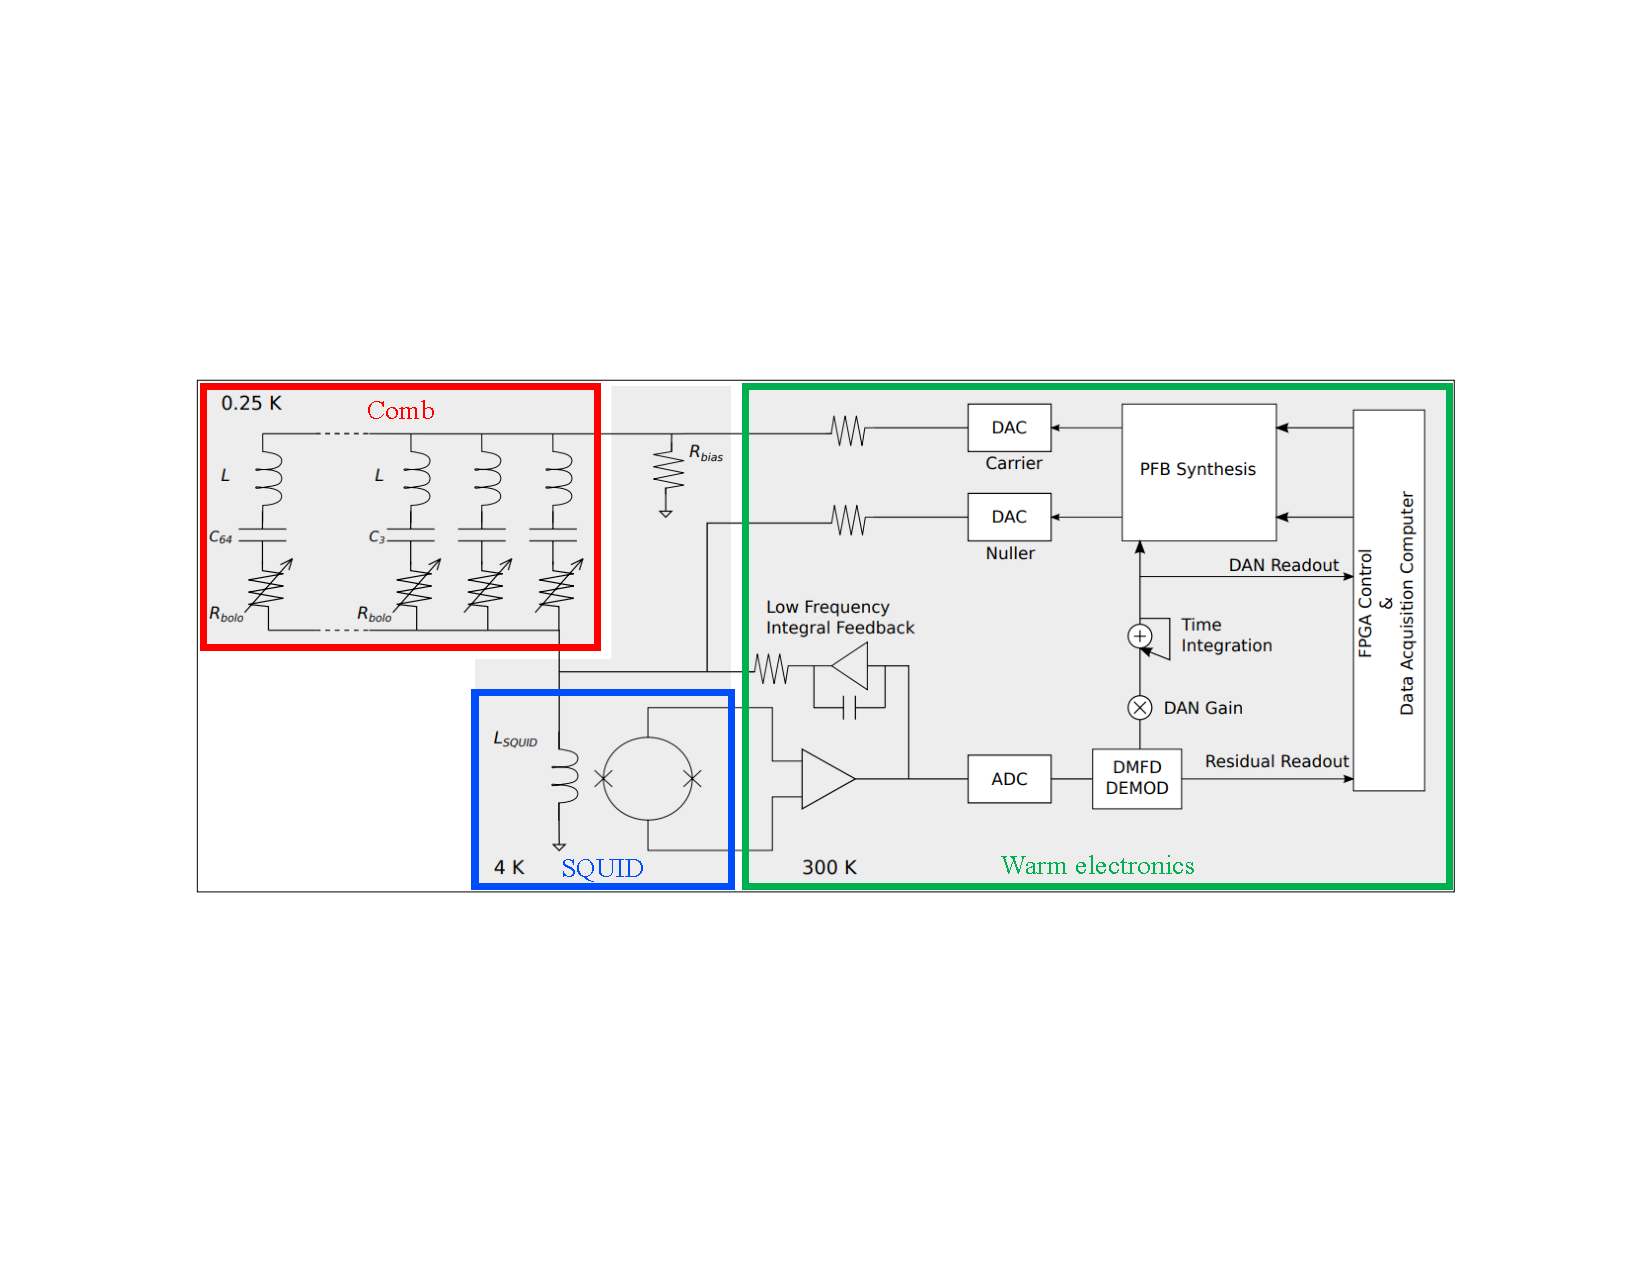
\includegraphics[width=\linewidth, trim=3cm 6.3cm 3cm 6.3cm, clip]{InstrumentOverview/Figures/dfmux_readout.pdf}
    \caption{Caption}
    \label{fig:dfmux_readout}
\end{figure}

SA's dfMUX scheme reads out 38 mK bolometers per 4~K SQUID at MHz frequencies. Each bolometer's bias/readout frequency is constructed by placing it in series with a tuned \important{LC resonator}, creating a ``comb'' of 38 low-impedance, non-overlapping ``peaks'' between 1~$\sim$~5~MHz. These frequency channels are then biased by a matching comb of AC waveforms, and when sky power changes on a given channel, this results in a change in the AC current across the bolometer. All 38 current waveforms are fed to one SQUID, are amplified into voltages, and are further amplified subsequently demodulated by a system of ambient electronics.

\begin{figure}[!t]
    \centering
    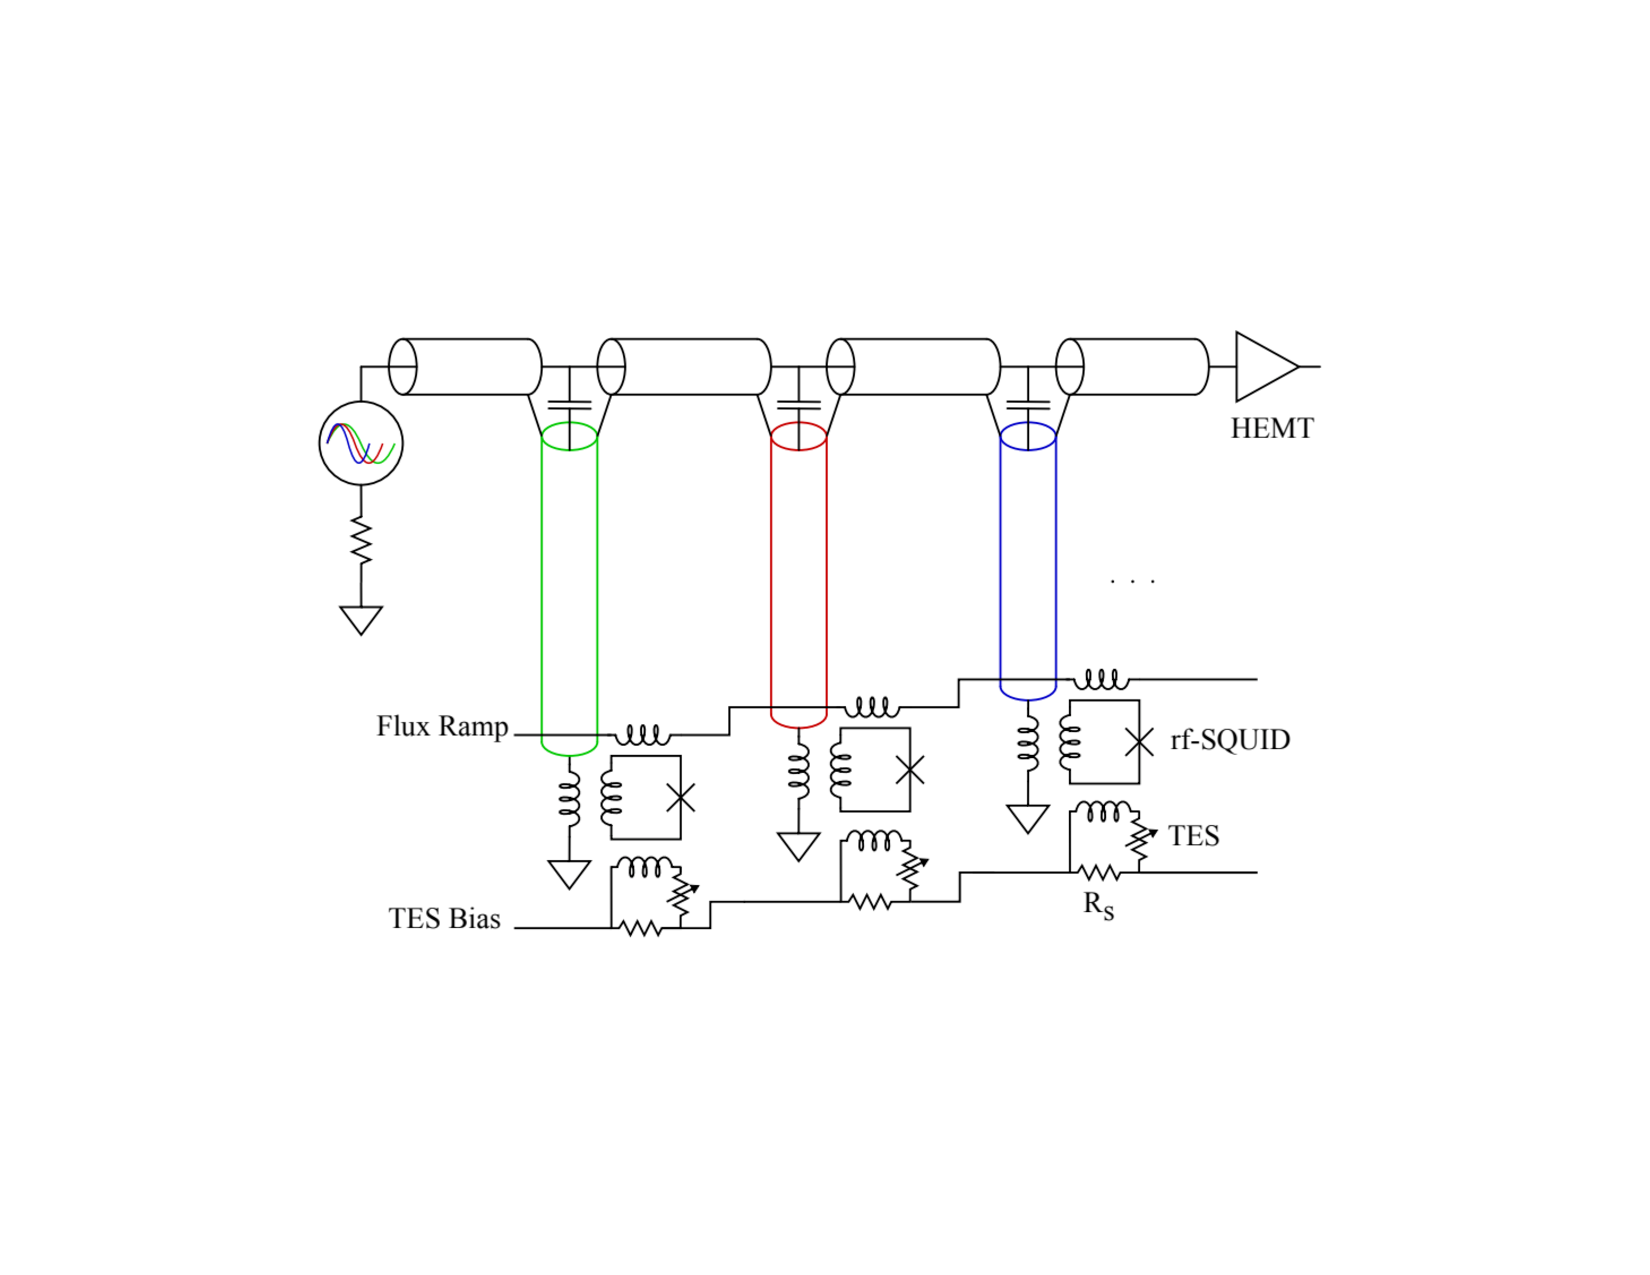
\includegraphics[width=\linewidth, trim=4cm 5.5cm 4cm 5cm, clip]{InstrumentOverview/Figures/umux_readout.pdf}
    \caption{Caption}
    \label{fig:umux_readout}
\end{figure}

SO's $\mathrm{\mu}$MUX scheme reads out $\sim$~1,000 mK bolometers coupled to $\sim$~1,000 mK SQUIDs (one SQUID per bolometer) per 4~K high-electron-mobility transistor (HEMT) amplifier at GHz frequencies. Instead of putting an LC resonator in series with the bolometer and using the same tone to both bias bolometer and sense its resistance changes, SO decouples the signal used to read out the bolometer and the signal used to bias it. As shown in Figure~blah, the TESes are biased with a DC voltage and are in series with an inductor. This inductor is coupled to a SQUID, which is in turn inductively coupled to an LC resonator. When the current across the bolometer changes, so does the SQUID-resonator effective inductance, in turn modulating the LC resonant frequency. When the resontator's impedance changes, so does the reflected signal, which is amplified by a broadband high-electron-mobility transistor (HEMT) amplifier and subsequently digitized by warm electronics. Because the probe (the LC resonator biases) and the bolometer voltage bias are separate in this scheme, $\mathrm{\mu}$MUX can operate at much higher frequencies and therefore multiplex more detectors on each amplifier.

While dfMUX and $\mathrm{\mu}$MUX are powerful techniques to read out the bolometer array, they have many challenges two of which are important for discussion to follow. First is bolometer responsivity, which is governed by its loop gain and depends heavily on implementation details, including the high-frequency impedances of the wiring, the effectiveness of the electromagnetic shielding, and the uniformity and consistency of the detector and resonator fabrication. Parasitic effects at high frequencies can be difficult to control and therefore can lead to substantial variations in how sky power is converted to analog-to-digital converter (ADC) counts. Second is readout noise, which depends on a plethora of factors, including SQUID noise, grounding quality, and detector bias parameters. Many of these factors are particularly prominent at higher frequencies and therefore are critical for dfMUX and $\mathrm{\mu}$MUX as opposed to other readout schemes (such as time-domain multiplexing). Because SA and SO push to very low thermal and optical noise, readout noise characterization and modeling are essential to an accurate assessment of instrument sensitivity.

%%%%%%%%%%%%%%%%%%%%%%%%%%%%%%%%
%%%%%%%%%%%%%%%%%%%%%%%%%%%%%%%%

\section{Technical objectives}


%%%%%%%%%%%%%%%%%%%%%%%%%%%%%%%%
%%%%%%%%%%%%%%%%%%%%%%%%%%%%%%%%
%%%%%%%%%%%%%%%%%%%%%%%%%%%%%%%%
%%%%%%%%%%%%%%%%%%%%%%%%%%%%%%%%

%\part{Noise modeling}

\chapter{Instrument Sensitivity}
\label{ch:cmb_instrument_sensitivity}

As overviewed in Section~\ref{sec:simons_array}, telescopes for observation of CMB polarization anisotropies are complex systems that rely on high-quality optical, thermal, and detection performance to be successful. Instrument performance is typically broken into two categories: \important{sensitivity} and \important{systematics}. Sensitivity is a simplistic measure of the instrument's signal to noise and relies, at its core, on only two factors: the amount of noise in your detectors, and the optical throughput of the system to a given signal on the sky. Sensitivity analyses typically assume a white noise spectrum (in other words, that all noise fluctuations are Gaussian, uncorrelated, and equal across all time scales) and a fixed sky signal. Systematics, on the other hand, are substantially more complex and involve effects such as optical sidelobes, intensity-to-polarization leakage, cross polarization, scan-synchronous signal, low-frequency noise, detector gain drift, focal plane temperature changes, readout pathologies, etc. In this sense, an accurate analyses of systematic effects requires a deep knowledge of the instrument and is a prerequisite to understanding not only system performance but the science data itself.

As detailed in Chapter~blah, a primary product of this dissertation is the development of a sensitivity calculator useful for both instrument design and forecasting and for instrument characterization. As a precursor to that discussion, we present the sensitivity calculation itself in this chapter, noting key advancements made as part of the presented research.

%%%%%%%%%%%%%%%%%%%%%%%%%%%%%%%%
%%%%%%%%%%%%%%%%%%%%%%%%%%%%%%%%
%%%%%%%%%%%%%%%%%%%%%%%%%%%%%%%%

\section{Noise spectrm}
\label{sec:sensitivity_noise_spectrum}

Sensitivity is often quantified in terms of the instrument's signal-to-noise ratio (SNR). In experiments that use photodetectors, such as mm-wave telescopes, SNR is often expressed in terms of \important{noise-equivalent power}, which is defined to be the signal power that gives a SNR of one given one Hz of output bandwidth. In this sense, NET is spectral quantity, and the amount of noise in a given sample depends on both the shape of the noise spectrum and on the integration bandwidth
\begin{equation}
    \left< \sigma_{\mathrm{P}}^{2} \right> = \int_{f_{\mathrm{lo}}}^{f_{\mathrm{hi}}} \left| \mathrm{NEP}(f) \right|^{2} \dd f \, ,
    \label{eq:net_spectrum_integrate}
\end{equation}
where here $f$ is \important{audio frequency} (in contrast to \textit{microwave frequencies}, which describe the vibrations of electromagnetic radiation).

When estimate the sensitivity of CMB instruments, the noise is often approximated to be ``white,'' or independent of frequency. In this case, the integral in Equation~\ref{eq:net_spectrum_integrate} becomes
\begin{equation}
    \left< \sigma_{\mathrm{P}}^{2} \right> = \left| \mathrm{NEP}\right|^{2} \Delta f \, ,
    \label{eq:net_white_spectrum}
\end{equation}
where $\Delta f$ is the \important{output bandwidth}. To understand the meaning of the output bandwidth, consider the Nyquist sampling theorem, which relates the \textit{maximum} integration bandwidth $\Delta f_{\mathrm{max}}$ to the sampling rate $1 / \Delta t_{\mathrm{samp}}$ as
\begin{equation}
    \Delta f_{\mathrm{max}} = \frac{1}{2 \Delta t_{\mathrm{samp}}} \, ,
    \label{eq:output_bandwidth_nyquist_frequency}
\end{equation}
When $\Delta f = f_{2} - f_{1} = f_{\max} - 0$, as is often the case when measuring an unmodulated signal, $f_{\mathrm{max}}$ is called the \important{Nyquist Frequency}.

NEP in CMB experiments is generally decomposed into photon noise, bolometer thermal noise, readout/amplifier noise, TES Johnson noise, and extraneous noise sources, each of which we detail in the sections to follow. These noise sources are typically assumed to be white and uncorrelated, meaning that they can be simulated independently and that their amplitudes add in quadrature. After estimating the NEP of a given detector output, it is then useful to estimate instrument signal to noise in terms of a given sky signal, which which is often given in temperature units and is referred to as \important{noise-equivalent temperature} (NET). NET is a common figure of merit for instrument sensitivity, and an accurate estimate relies on an accurate understanding of many aspects of the instrument, including the ambient optical environment, telescope + receiver optical throughput, bolometer and SQUID noise, spillover both inside and outside of the cryostat, and beam coupling efficiency (see Equation~\ref{eq:beam_coupling_efficiency}).

%%%%%%%%%%%%%%%%%%%%%%%%%%%%%%%%
%%%%%%%%%%%%%%%%%%%%%%%%%%%%%%%%
%%%%%%%%%%%%%%%%%%%%%%%%%%%%%%%%

\section{Photon statistics}
\label{sec:sensitivity_photon_statistics}

As briefly alluded to in Section~\ref{sec:sensitivity_optical_power_detail}, it is often convenient to describe the propagation of radiation through the optical system to the detector in terms of \important{modes}. A single mode of the electric field is given by
\begin{equation}
    E_{p}(\vec{r}, t) = E_{0} \sin \left( \vec{k} \cdot \vec{r} - \omega t \right) \, ,
    \label{eq:electromagnetic_mode}
\end{equation}
where $\vec{r}$ is position, $t$ is time, $\vec{k} = (2 \pi \nu / c) \hat{k}$ is the wave vector, $\omega = c k$ is the light's angular frequency, and the index $p$ denotes a single polarization. The important characteristic of an electromagnetic mode is that it is described by a single vibrational component of microwave frequency $\nu$ and is therefore best represented in frequency space.

The quantum mechanical analog to electromagnetic modes are \important{coherent states}, which, as the name suggests, is a basis of full coherence. Coherent states are eigenvectors of the photon creation operator $a^{\dagger}_{\vec{k} p}$
\begin{equation}
    a^{\dagger}_{\vec{k} p} \left| \alpha_{\vec{k} p} \right> = \alpha_{\vec{k} p} \left| \alpha_{\vec{k} p} \right> \, .
    \label{eq:coherent_state_eigenbasis}
\end{equation}
It is also useful to define the electric field operator as
\begin{equation}
    \hat{E}_{p}^{(+)}(\vec{r}, t) \left| \alpha_{\vec{k} p} \right> = E_{p}(\vec{r}, t) \left| \alpha_{\vec{k} p} \right> \, ,
    \label{eq:electric_field_operator_definition}
\end{equation}
where here, the classical quantity $E_{p}(\vec{r}, t)$ is the observable quantity. Given Equations~\ref{eq:coherent_state_eigenbasis} and~\ref{eq:electric_field_operator_definition}, we can relate the electric field operator for a single electromagnetic mode to the photon operator for a coherent state as
\begin{equation}
    \hat{E}_{p}^{(+)}(\vec{r}, t) = \sqrt{\frac{\hbar \omega}{2 \varepsilon_{0} v}} a_{\vec{k} p}^{\dagger} \sin(\vec{k} \cdot \vec{r} - \omega t) \, ,
    \label{eq:electric_field_operator_single_mode}
\end{equation}
where here $\hbar$ is the reduce Planck constant, $\varepsilon_{0}$ is the permittivity of free space, $v$ is the volume of space of interest. Equation~\ref{eq:electric_field_operator_single_mode} show that by understanding the quantum fluctuations of the \textit{quantum} coherent state $\left| \alpha_{\vec{k} p} \right>$, we can understand the photon noise in a \textit{classical} field $E_{p}(\vec{r}, t)$.

In order to study the statistics of thermal light, we can assume that the probability of finding a photon is governed by the Boltzmann probability distribution
\begin{equation}
    P_{n} = \frac{\exp \left( - E_{n} / k_{\mathrm{B}} T \right)}{\sum_{n = 0}^{\infty} \exp \left( - E_{n} \ k_{\mathrm{B}} T \right)} \, ,
    \label{eq:boltzmann_distribution}
\end{equation}
where the energy of the harmonic oscillator state $n$ is given by
\begin{equation}
    E_{n} = \left( n + \frac{1}{2} \right) \hbar \omega \, ,
    \label{eq:harmonic_oscillator_energy}
\end{equation}
and where here, again is related to microwave frequency as $\omega = 2 \pi \nu$. Noting that the zero-point energy cancels out when Equation~\ref{eq:harmonic_oscillator_energy} is substituted into Equation~\ref{eq:boltzmann_distribution}, it is convenient to define the factor 
\begin{equation}
    U = \exp \left(- \hbar \omega / k_{\mathrm{B}} T \right) \, ,
    \label{eq:boltzmann_energy_factor}
\end{equation}
such that the probability distribution can be rewritten as 
\begin{equation}
    P_{n} = \frac{U^{n}}{\sum_{n = 0}^{\infty} U^{n}} = \left( 1 - U \right) U^{n} \, ,
    \label{eq:boltzmann_probability_simplified}
\end{equation}
where we have invoked the geometry series relation $\sum_{n = 0}^{\infty} U^{n} = (1 - U)^{-1}$. Given this simplified form for the probability distribution, we can calculate the mean photon occupation number as
\begin{equation}
    \left< n \right> = \sum_{n = 0}^{\infty} n P_{n} = \left( 1 - U \right) \sum_{n = 0}^{\infty} n U^{n} = \frac{U}{1 - U} \, ,
    \label{eq:mean_photon_count_probability_distribution}
\end{equation}
where we have used the relation $\sum_{n} n U^{n} = U \partial / \partial U \sum_{n} U^{n}$ and have once again invoked the geometry series relation $\sum_{n = 0}^{\infty} U^{n} = (1 - U)^{-1}$. Substituting Equation~\ref{eq:boltzmann_energy_factor} into Equation~\ref{eq:mean_photon_count_probability_distribution} gives the mean photon number for thermal light of temperature $T$ at frequency $\omega$
\begin{equation}
    \left< n \right> = \frac{1}{\exp \left( \hbar \omega / k_{\mathrm{B}} T \right) - 1} \, ,
    \label{eq:photon_occupation_number}
\end{equation}
which is the familiar \important{Bose-Einsten distribution}.

\begin{figure}[!t]
    \centering
    \subfloat[\label{fig:photon_statistics:a}]{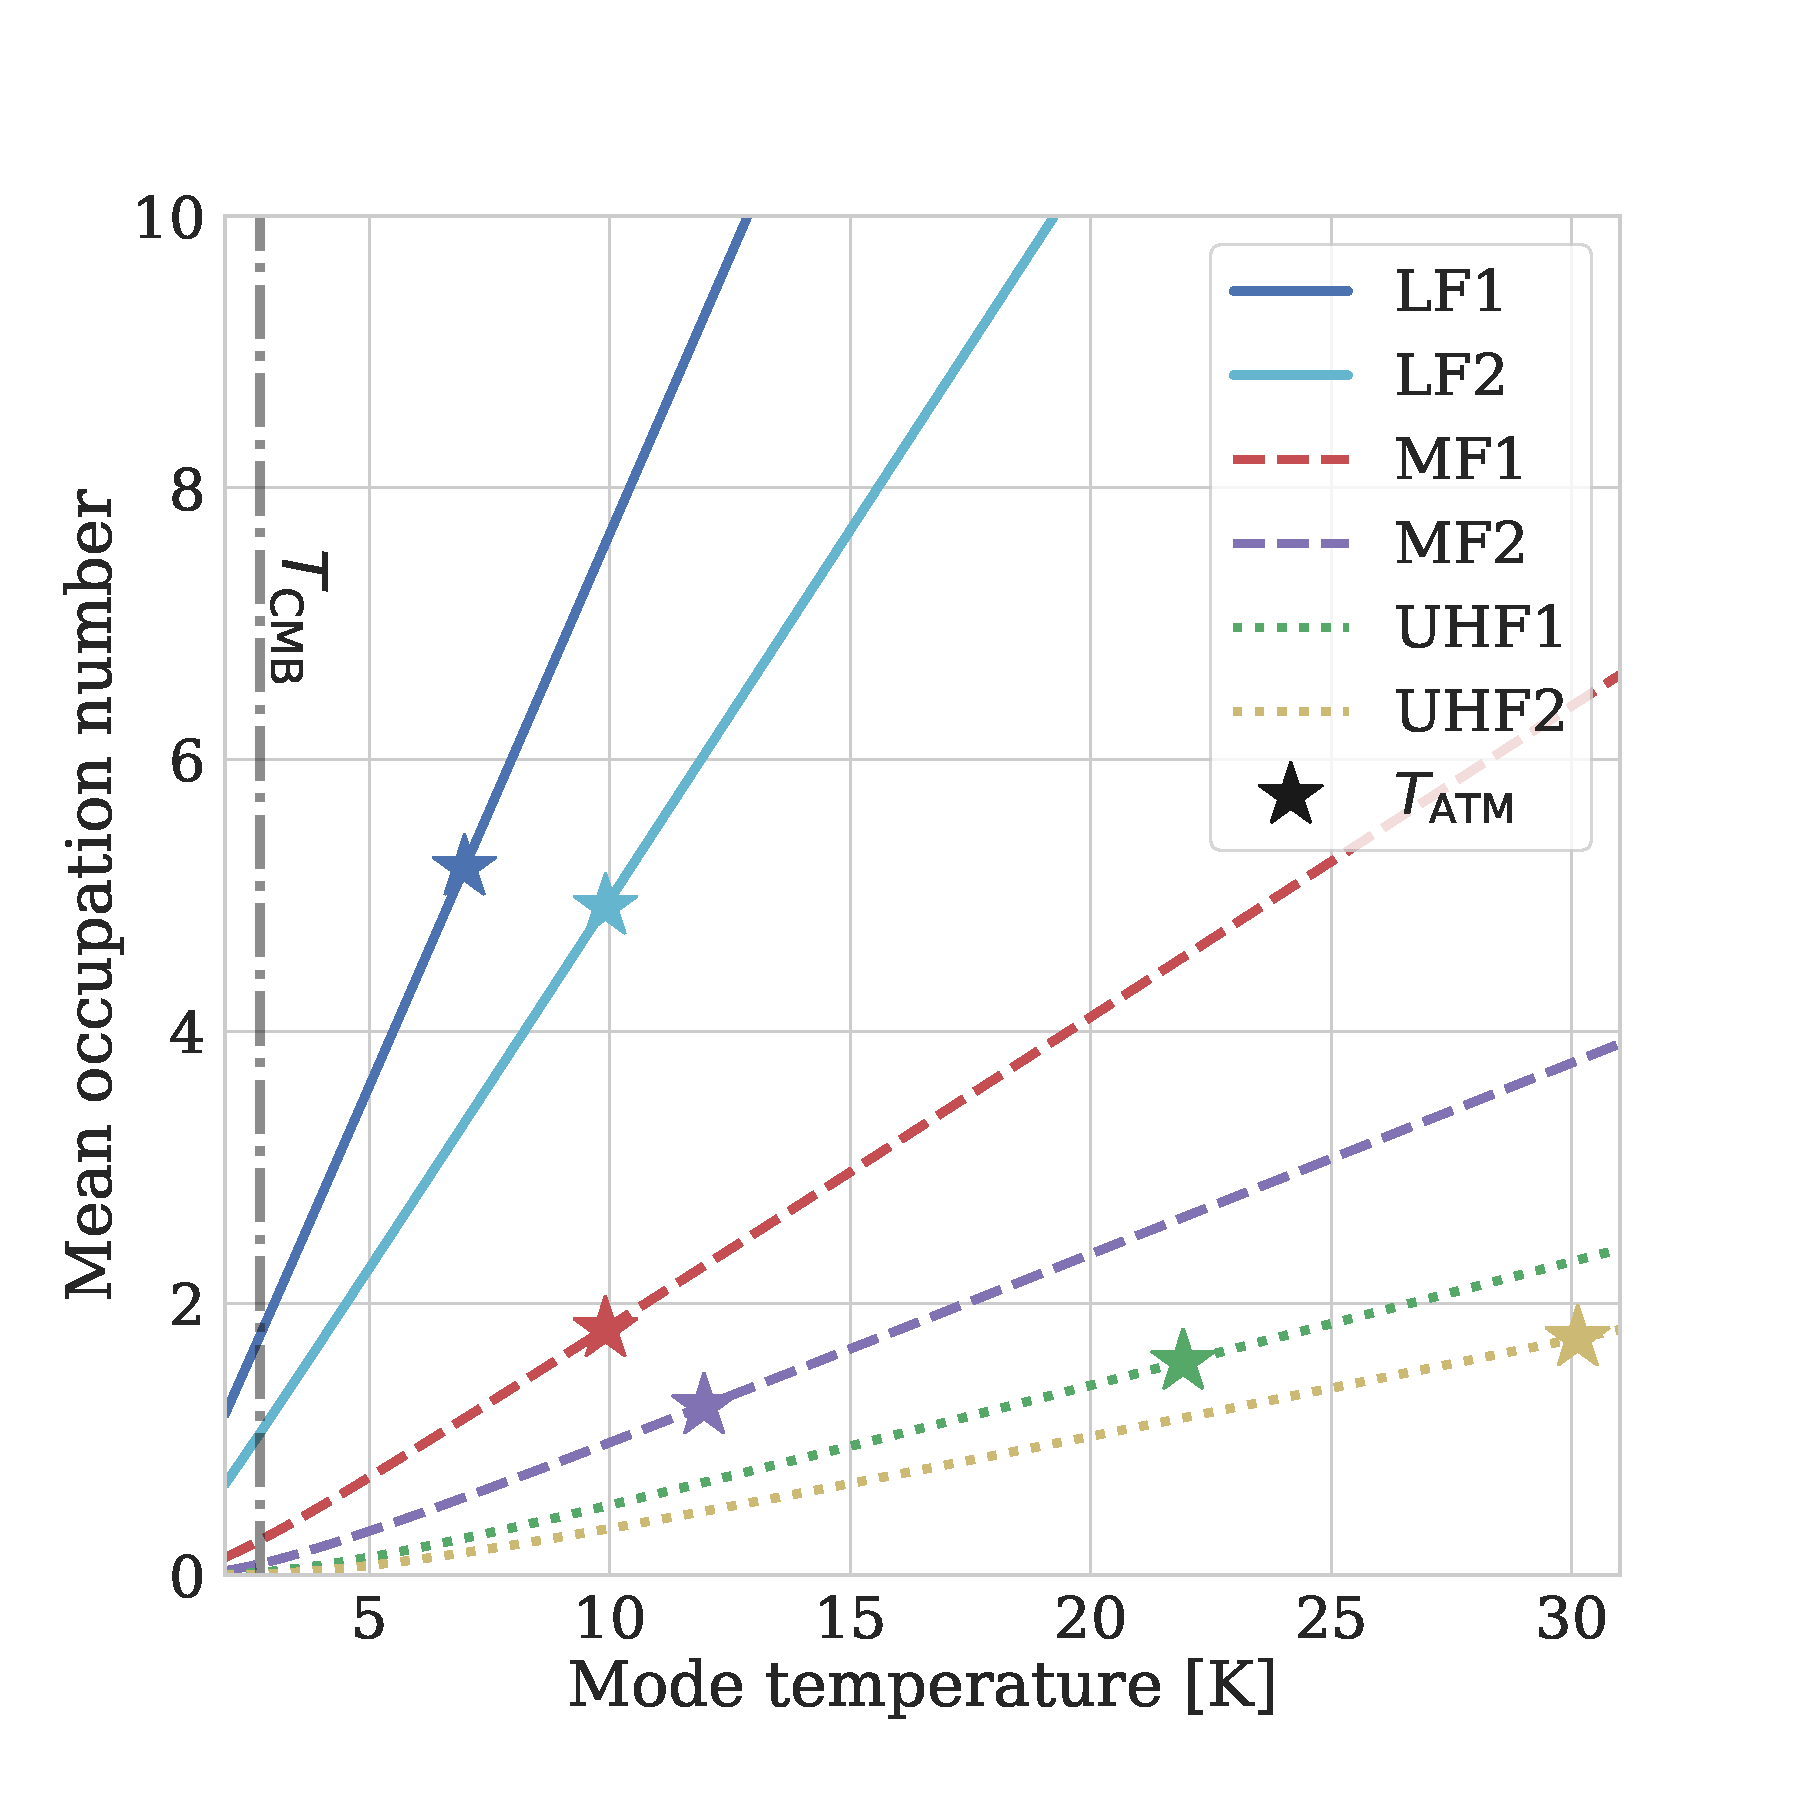
\includegraphics[width=0.48\linewidth, trim=0cm 1cm 2cm 3cm, clip]{SensitivityCalculation/Figures/mean_occupation_number.pdf}}
    \subfloat[\label{fig:photon_statistics:b}]{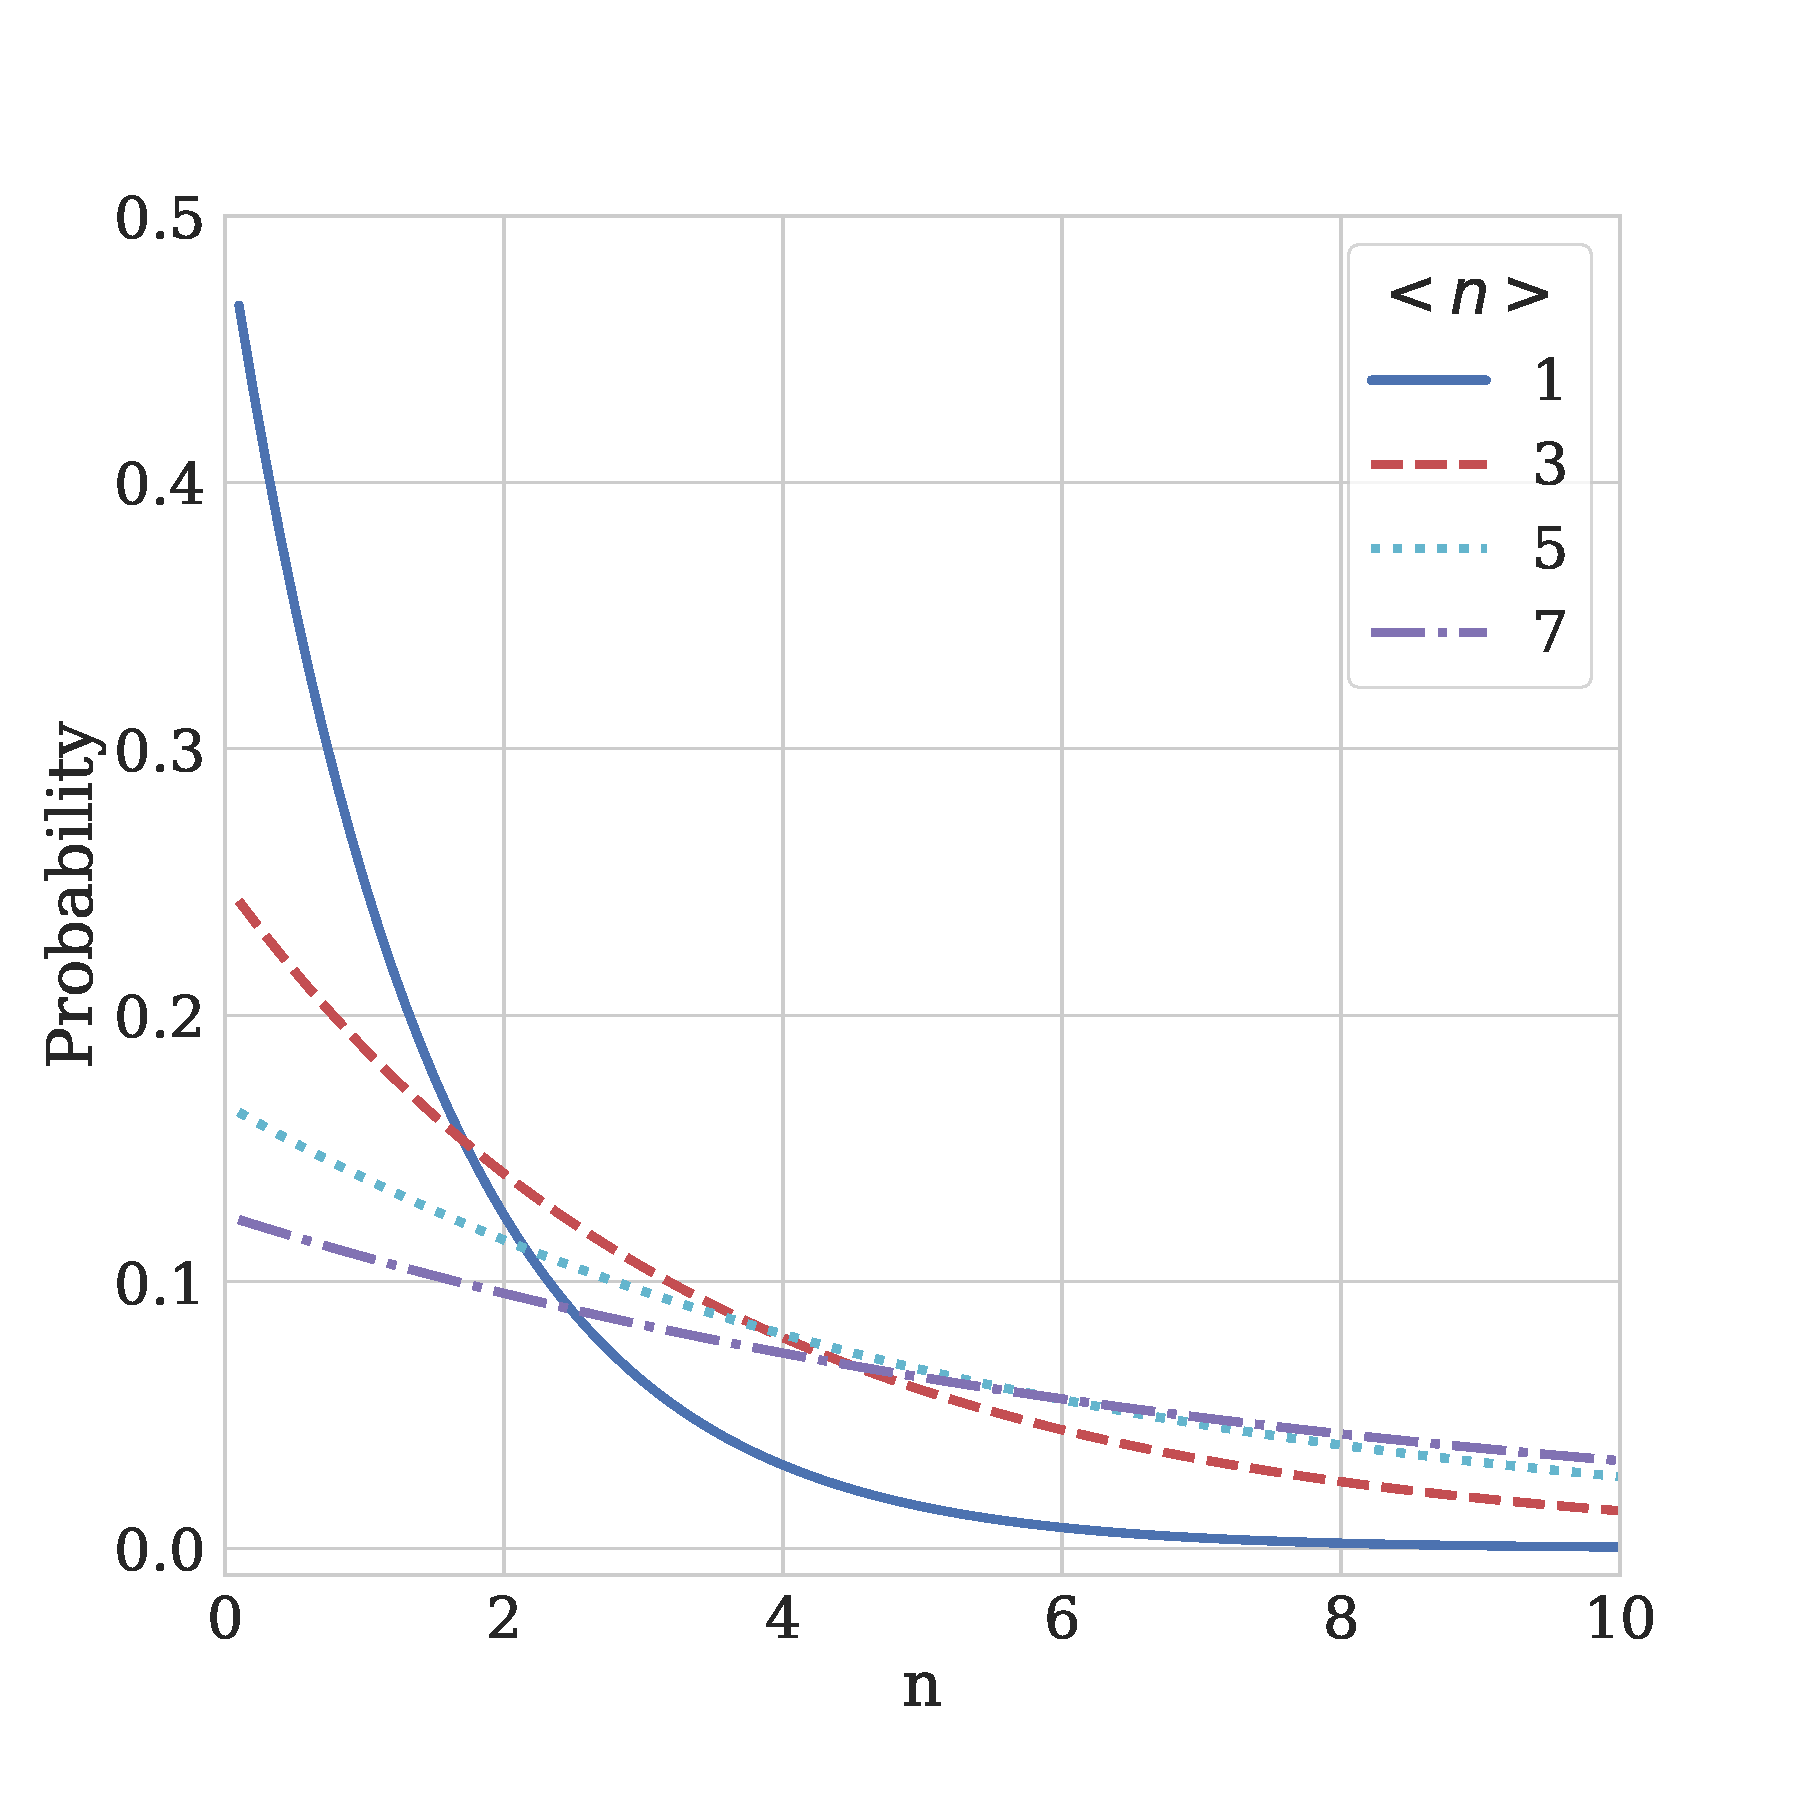
\includegraphics[width=0.48\linewidth, trim=0cm 1cm 2cm 3cm, clip]{SensitivityCalculation/Figures/occupation_number_distribution.pdf}}
    \caption{(a) is the mean occupation number vs mode temperature integrated over the SO bands. The atmospheric temperature for each band is marked with a star, and the CMB temperature is marked with a vertical line. (b) is the probability distribution vs mode number for various mean occupation numbers. The probability broadens with increasing $\left< n \right>$, which in turn gives rise to larger mode fluctuations, while at smaller $\left< n \right>$ the distribution looks increasingly Poissonian.}
    \label{fig:my_label}
\end{figure}

Now that we have an expression for the \textit{mean} photon count, we move to find an expression for the RMS photon count fluctuations
\begin{equation}
    \left( \Delta n \right)^{2} = \sum_{n} \left(n - \left< n \right> \right)^{2} P_{n} = \left< n ^{2} \right> - \left< n \right>^{2} \, .
    \label{eq:photon_variance_probability_distribution}
\end{equation}
In order to simplify this expression, it is useful to rewrite $P_{n}$ by plugging $U = \left< n \right> \ (1 + \left< n \right>)$ into Equation~\ref{eq:boltzmann_probability_simplified} to obtain
\begin{equation}
    P_{n} = \frac{\left< n \right>^{n}}{\left( 1 + \left< n \right> \right)^{1 + n}} \, .
    \label{eq:boltzmann_probability_in_terms_of_mean}
\end{equation}
In addition, it is useful to write the $P_{n}$ in terms of its \textit{factorial moments}
\begin{equation}
    \left< \frac{n !}{\left( n - r \right) !} \right> = \sum_{n} n \left( n - 1 \right) \left( n - 2 \right) ... \left( n - r + 1 \right) P_{n} = r ! \left< n \right>^{r} \, ,
    \label{eq:factorial_moments_boltzmann}
\end{equation}
where the last equality comes from plugging Equation~\ref{eq:boltzmann_probability_in_terms_of_mean} in for $P_{n}$ (citation needed for Loudon). We can then use Equation~\ref{eq:factorial_moments_boltzmann} with $r = 2$ to find
\begin{equation}
    \left< n (n - 1) \right> = 2 \left< n \right>^{2} \, ,
    \label{eq:factorial_second_moment}
\end{equation}
which can finally be plugged into Equation~\ref{eq:photon_variance_probability_distribution} to obtain the relation
\begin{equation}
    \left( \Delta n \right)^{2} = \left< n \right> + \left< n \right>^{2} \, .
    \label{eq:photon_count_fluctuations}
\end{equation}
When the mean photon occupation number is $\left< n \right> \ll 1$, which is true when $\hbar \omega \gg k_{\mathrm{B}} T$, Equation~\ref{eq:photon_count_fluctuations} reduces to $\left( \Delta n \right)^{2} \approx \left< n \right>$, which is true of a Poisson distribution. Therefore, in the high-frequency and/or low-temperature limit, photon noise is \important{shot noise} and fluctuations are uncorrelated. On the other hand, when the occupation is $\left< n \right> \gg 1$, which is true when $\hbar \omega \ll k_{\mathrm{B}} T$, Equation~\ref{eq:photon_count_fluctuations} reduces to $\left( \Delta n \right)^{2} \approx \left< n \right>^{2}$, which is true of an exponential distribution. Therefore, in the low-frequency and/or high-temperature limit, photon noise is (what is often called) \important{Bose noise} and fluctuations are, in general, correlated.

%%%%%%%%%%%%%%%%%%%%%%%%%%%%%%%%
%%%%%%%%%%%%%%%%%%%%%%%%%%%%%%%%
%%%%%%%%%%%%%%%%%%%%%%%%%%%%%%%%

\section{Photon NEP}
\label{sec:sensitivity_photon_nep}

According to Equation~\ref{eq:photon_count_fluctuations}, the variance of the photon occupation number for a given mode is determined solely by the mean occupation number. In this section, we relate those photon count statistics to those of optical power and outline the calculation of photon NEP.

Under the assumption that each optic is an isothermal blackbody, the power spectral density $p_{i}(\nu)$ for optical element $i$ is determined by its physical temperature $T_{i}$, the aggregate transmissivity of all optics between it and the detector $\left[ \eta_{i+1} (\nu) , \ldots , \eta_{N_{\mathrm{elem}}} (\nu) \right]$, its emissivity $\epsilon_{i} (\nu)$, its spillover fraction $\beta_{i} (\nu)$, the effective temperature of the spillover radiation $T_{\beta ; i}$, its scattering fraction $\delta_{i} (\nu)$, and the effective temperature of the scattered radiation $T_{\delta ; i}$
\begin{align}
    p_{i} \left( \nu \right) =
    \prod_{j = i + 1}^{N_{\mathrm{elem}}} \eta_{j} (\nu) \left[ \epsilon_{i} (\nu) S(T_{i}, \nu) + \beta_{i}(\nu) S(T_{\beta;i}, \nu) + \delta_{i}(\nu) S(T_{\delta; i}, \nu) \right] \, .
    \label{eq:pow_spec_density}
\end{align}
Here, the power spectral density function $S(T, \nu)$ of the emitted, scattered, and spilled power from each element into a mode with frequency $\nu$ is given by the Planck spectral density
\begin{equation}
    S(T, \nu) = A \Omega \frac{h \nu^{3}}{c^{2}} n(T, \nu) = h \nu n(T, \nu) \, ,
    \label{eq:planck_spectrum}
\end{equation}
where $n(T, \nu)$ is the Bose occupation number defined in Equation~\ref{eq:photon_occupation_number}, and where for a diffraction-limited, single-moded detector, the entendue $A \Omega$ is given by the square of the detected wavelength
\begin{equation}
    A \Omega = \left( \frac{c}{\nu} \right)^{2} = \lambda^{2} \, .
    \label{eq:aomega}
\end{equation}

For a single mode governed by a single blackbody source with a single temperature, power fluctuations are 
\begin{equation}
    \left(\Delta P_{\mathrm{mode}} \right)^{2} = \left(h \nu \right)^{2} \left( \left< n \right> + \left< n \right>^{2} \right) \, .
    \label{eq:photon_power_fluctuations_single_mode}
\end{equation}
Generalizing this relation to encompass all modes within the entendue $A \Omega$ and across all frequencies gives us the photon NEP for bolometeric detection
\begin{equation}
    \mathrm{NEP}_{\mathrm{ph}} = \sqrt{2 \int_{0}^{\infty} \left[ h \nu \sum_{i=1}^{N_{\mathrm{elem}}} p_{i} (\nu) + \left( \sum_{i=1}^{N_{\mathrm{elem}}} p_{i} (\nu) \right)^{2} \right] B^{2}(\nu) \mathrm{d} \nu} \, .
    \label{eq:nep_ph}
\end{equation}
where $\nu$ is microwave frequency, $p_{i}(\nu)$ is the power spectral density of optical element $i$ at the detector input, the summation contains all $N_{\mathrm{elem}}$ optical elements including the sky, telescope, and camera, and $B(\nu)$ is the detector transmissivity vs. frequency, also called the \important{detector band}. This relation is often approximated as
\begin{equation}
    \mathrm{NEP_{ph}} \approx \sqrt{2 \left[ h \nu_{\mathrm{c}} P_{\mathrm{opt}} + \frac{P_{\mathrm{opt}}^{2}}{\Delta \nu} \right]} \, ,
\end{equation}
where $\nu_{\mathrm{c}}$ and $\Delta \nu$ are the central frequency and bandwidth of the detector band $B(\nu)$, where the total detected optical power is
\begin{equation}
    P_{\mathrm{opt}} = \int_{0}^{\infty} \left[ \sum_{i=1}^{N_{\mathrm{elem}}} p_{i}(\nu) \right] B(\nu) \mathrm{d} \nu \, ,
    \label{eq:popt}
\end{equation}
and where the approximation remains valid in the Rayleigh-Jeans limit $h \nu \ll k_{\mathrm{B}} T$.

%%%%%%%%%%%%%%%%%%%%%%%%%%%%%%%%
%%%%%%%%%%%%%%%%%%%%%%%%%%%%%%%%
%%%%%%%%%%%%%%%%%%%%%%%%%%%%%%%%

\section{Optical power}
\label{sec:sensitivity_optical_power}

As shown in Section~\ref{sec:sensitivity_photon_nep}, calculating photon noise comes down to an accurate understanding of $p(\nu)$, which is defined in Equation~\ref{eq:pow_spec_density} and is governed by emissivity, spillover, scattering, and transmissivity. In this section, we detail how $p(\nu)$ is calculated.

\begin{figure}
    \centering
    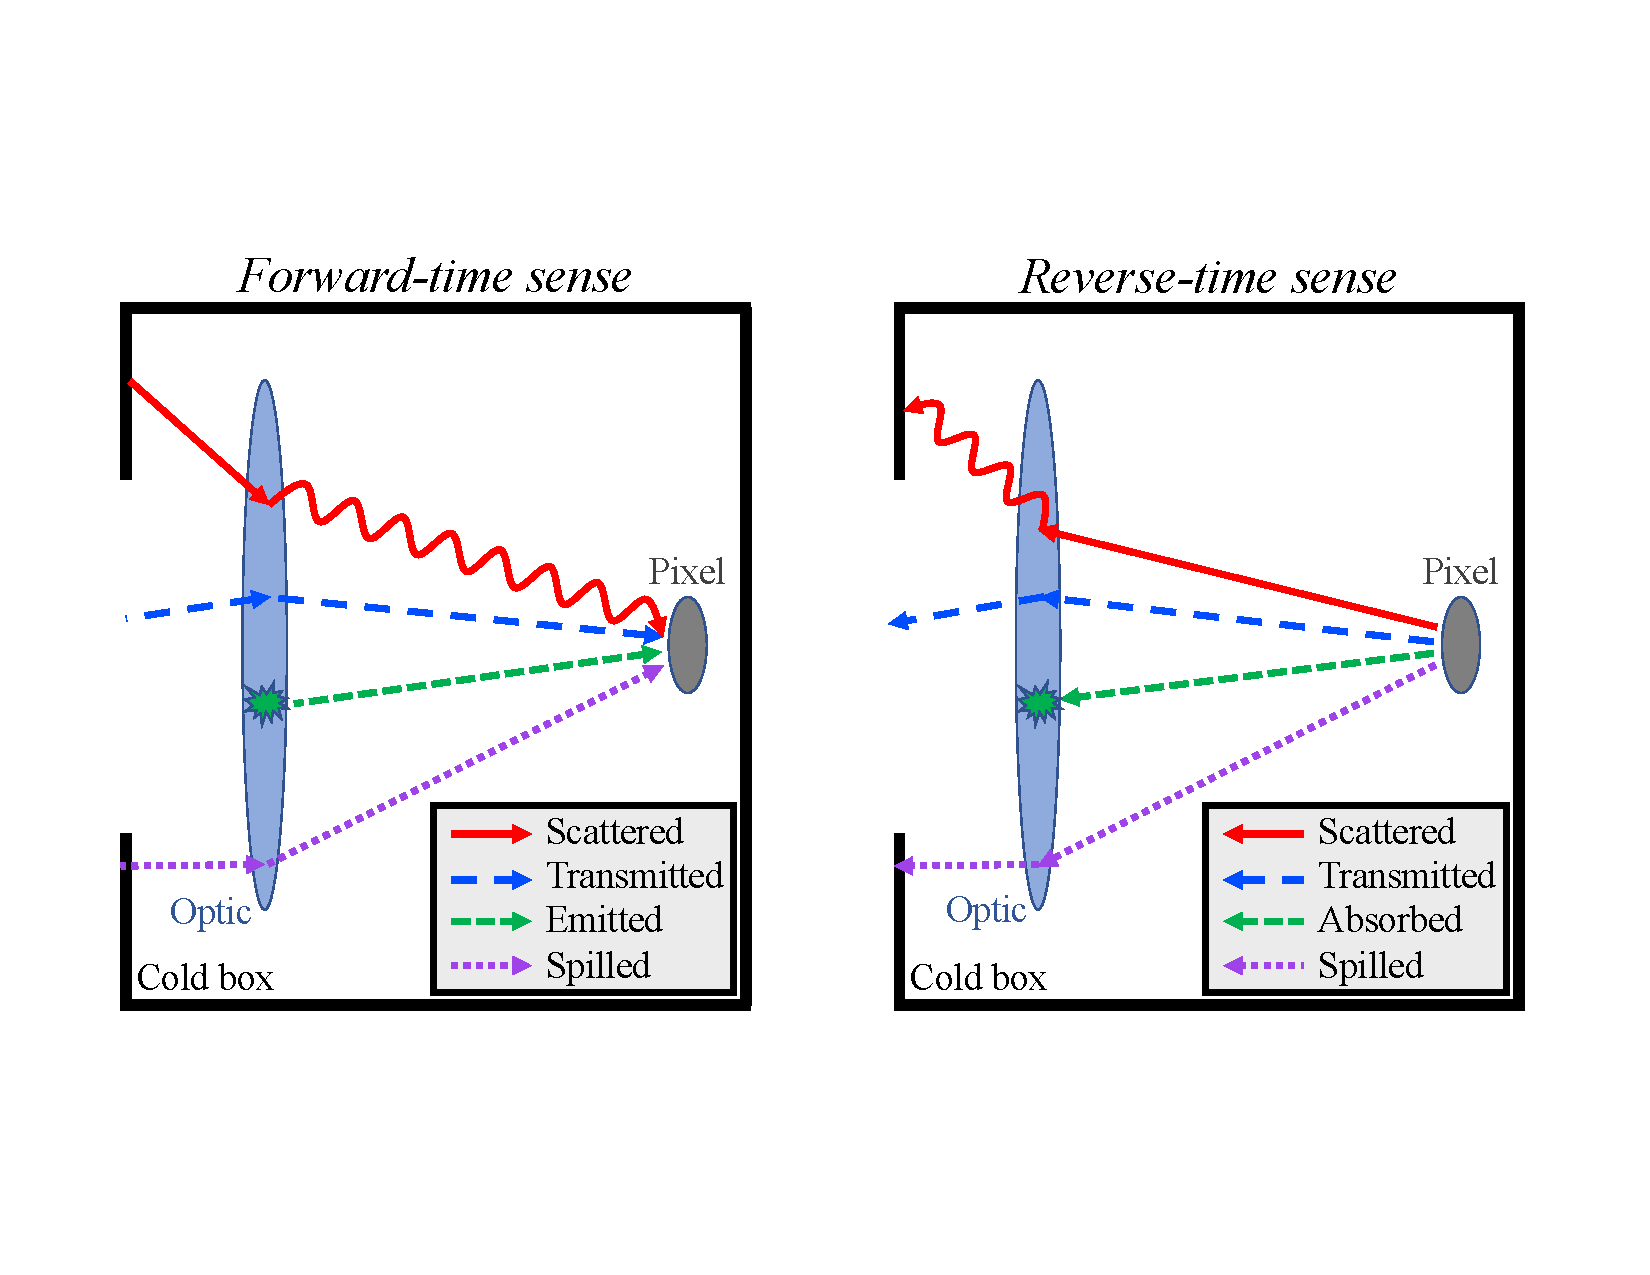
\includegraphics[width=\linewidth, trim=2cm 4cm 2cm 4cm, clip]{SensitivityCalculation/Figures/reverse_time_sense.pdf}
    \caption{A schematic to visually demonstrate the concept of reverse-time sense calculations as they apply to transmissivity, absorptivity/emissivity, scattering fraction, and spillover fraction. Most often when estimating sensitivities, it is useful to think in the reverse-time sense, or in the paradigm of the detector pixel emitting towards the sky.}
    \label{fig:reverse_time_sense}
\end{figure}

Assume that the optical stack, which comprises the telescope's mirrors, the receiver's lenses and filters, and the focal plane's optics, can be represented as a one-dimensional array of blackbody absorbers/emitters/attenuators in thermal equilibrium. While such a situation is not in general true, as temperature gradients develop across optics and IR loads and fridge performance vary in time, it is a reasonable approximation for the NET calculation, which is a white-noise estimate. There are four primary components to the optical load on the detector, and for each, it is most useful to think in the time-reverse sense.

%%%%%%%%%%%%%%%%%%%%%%%%%%%%%%%%
%%%%%%%%%%%%%%%%%%%%%%%%%%%%%%%%

\subsection{Emissivity and absorptivity}
\label{sec:sensitivity_emissivity}

\important{Emissivity} is the propensity of an optical element to emit mm-wave radiation. For dielectrics, the emissivity is determined by its loss tangent
\begin{equation}
    \tan \delta = \frac{2 \pi \nu \varepsilon'' + \sigma}{2 \pi \omega \varepsilon'} \approx \frac{\varepsilon''}{\varepsilon'} \, ,
    \label{eq:loss_tangent}
\end{equation}
where $\sigma$ is the conductivity, the dielectric constant is
\begin{equation}
    \varepsilon = \varepsilon' - i \varepsilon'' \, ,
    \label{eq:dielectric_constant}
\end{equation}
and the approximation applies for low-loss materials where $\varepsilon'' \ll \varepsilon'$. The emissivity of the dielectric can then be written as
\begin{equation}
    \epsilon_{\mathrm{diel}}(\nu) = 1 - \exp \left( - \frac{2 \pi \nu n t}{c} \tan \delta \right) \approx -\frac{2 \pi \nu t}{c} \tan \delta \, ,
    \label{eq:dielectric_emissivity}
\end{equation}
where $t$ is the optical thickness, $c$ is the speed of light in a vacuum, $n$ is the refractive index of the dielectric, and the approximation applies in the limit of a small loss tangent.

For conductors, such as mirrors, emissivity is generated by Ohmic losses
\begin{equation}
    \epsilon_{\mathrm{cond}}(\nu) = 1 - 4 \sqrt{\frac{\pi \nu \mu_{0}}{\sigma}} \, ,
    \label{eq:ohmic_loss_emissivity}
\end{equation}
where $\sigma$ is the conductivity and $\mu_{0}$ is the permeability of free space. Note that this equation assumes normal incidence, and at oblique angles, conductors skin depth is different for the S and P polarizations, which gives rise to slight differences in emissivities for different polarizations. While such small effects are indeed an important systematic effect for an accurate extraction of CMB polarization fluctuations, they are not important for sensitivity, which is concerned with spatially and polarization-averaged loading estimates.

Under the assumption that each optical element is a blackbody, its emission results from the thermodynamic motions of its composing molecules, which are Gaussian random and wide-band (as opposed to more complex materials with feature-filled emission spectra). In this paradigm, it is a very good assumption that the emissivity and absorptivity are equivalent
\begin{equation}
    \alpha(\nu) \equiv \frac{P_{\mathrm{abs}}}{P_{\mathrm{in}}} = \epsilon(\nu) \, .
    \label{eq:emissivity_absorptivity_equivalence}
\end{equation}
Therefore, not only does dielectric emission lead to parasitic loading, but it also leads to signal attenuation.

%%%%%%%%%%%%%%%%%%%%%%%%%%%%%%%%
%%%%%%%%%%%%%%%%%%%%%%%%%%%%%%%%

\subsection{Spillover fraction}
\label{sec:sensitivity_spillover_fraction}

\important{Spillover fraction} is the fraction of incident power that spills over the diffraction-limited area of a given optical element
\begin{equation}
    \beta(\nu) \equiv \frac{P_{\mathrm{spill}}(\nu)}{P_{\mathrm{in}}(\nu)} \, ,
    \label{eq:spillover_fraction_definition}
\end{equation}
where again, $P_{\mathrm{in}}(\nu)$ and $P_{\mathrm{spill}}(\nu)$ are in general frequency-dependent. Spillover fraction is most easily imagined in the reverse-time sense, from the perspective of the detector radiating towards the sky. If some power from a given pixel falls outside the ``imaged'' region of any optical element, this radiation will not propagate to the sky but will instead terminate somewhere else. Given that the detector can ``see'' these non-optical regions, then, flipping into the forward time sense, photons emitted from these non-optical regions are detected, which gives rise to optical power on the bolometer. 

The intensity of the spillover radiation is in turn governed by the \important{effective temperature of the spillover radiation} $T_{\beta}$. Often times in CMB experiments, when radiation spills over an optic (in the reverse-time sense), it ``lands'' on some surface. For example, if the spill is over the Lyot, that surface would be the stop, or if the spill is over a lens, that surface would be somewhere in the cryostat, or if the spill is over the primary mirror, that surface could be either the sky or the ground. The aggregate radiation from these surfaces is most conveniently described by an \textit{effective temperature}, which is often defined as
\begin{equation}
    T_{\mathrm{eff}} \equiv \varepsilon_{\mathrm{surface}} T_{\mathrm{surface}} \, ,
    \label{eq:effective temperature}
\end{equation}
where $T_{\mathrm{surface}}$ the surface's physical temperature and $\varepsilon$ is its emissivity. The astute reader will note that plugging $T_{\mathrm{eff}}$ into the Planck spectrum is not the same as using the spectrum for $T_{\mathrm{phys}}$ modified by the emissivity $\varepsilon{\mathrm{surface}}$. However, the equivalence is sufficient in the Rayleigh-Jeans limit, which often suffices for the CMB instrument calculations to follow.

%%%%%%%%%%%%%%%%%%%%%%%%%%%%%%%%
%%%%%%%%%%%%%%%%%%%%%%%%%%%%%%%%

\subsection{Scattering fraction}
\label{sec:sensitivity_scattering_fraction}

\important{Scattering fraction} is the fraction of incident power that is scattered by a given optical element
\begin{equation}
    \delta(\nu) \equiv \frac{P_{\mathrm{scatt}}(\nu)}{P_{\mathrm{in}}(\nu)} \, .
    \label{eq:scattering_fraction_definition}
\end{equation}
In a similar sense to spillover, scattering fraction is most easily imagined in the reverse-time sense, from the perspective of the detector radiating towards the sky. If some power from a given pixel is scattered by an optical element, this radiation will not propagate to the sky but will instead terminate onto some surface that will, in the forward-time sense, emit optical power on the bolometer. The intensity of the scattered radiation is also governed by the \important{effective temperature of the scattered radiation} $T_{\delta}$ and therefore also follows Equation~\ref{eq:effective temperature}.

There are many mechanisms for scattering, but the two most common in mm-wave experiments are Mie scattering and Ruze scattering. Mie scattering arises due to any irregularity in an otherwise homogeneous (or well-ordered) medium. Common examples in CMB telescopes are voids in dielectric substrates, air bubbles/gaps between anti-reflection coating layers, and sub-wavelength filler materials. In the limit that the scattering center is much smaller than the wavelength, which is often a good approximation in mm-wave telescopes, the Mie scattering is well-described by the Rayleigh scattering cross section
\begin{equation}
    \sigma_{\mathrm{Ray}} \equiv \frac{2 \pi^{5}}{3} \frac{d^{6}}{\lambda^{4}} \left( \frac{n_{2}^{2} - n_{1}^{2}}{n_{2}^{2} + 2 n_{1}^{2}} \right)^{2} \, ,
    \label{eq:rayleigh_scattering_cross_section}
\end{equation}
where $d$ is the diameter of the particle/void/deformity, $n_{2}$ is its refractive index, and $n_{1}$ is the refractive index of the medium. The aggregate impact of Rayleigh scatterers is then given by the Beer-Lambert Law
\begin{equation}
    \beta(\nu) = 1 - \exp \left( - \sigma_{\mathrm{Ray}} N z \right) \, ,
    \label{eq:beer_lambert_law}
\end{equation}
where $N$ is the number density of scatterers and $z$ is the optical path length of the scattering medium. Scattering is also a very important sensitivity parameter to calculate, characterize, and understand, especially because it does not improve with decreasing temperature, unlike dielectric loss.

Scattering from reflectors is typically due to their surface roughness and is quantified by Ruze scattering
\begin{equation}
    \beta_{\mathrm{Ruze}}(\nu) = 1 - \exp \left[ \left( \frac{4 \pi \sigma \nu}{c} \right)^{2} \right] \, ,
    \label{eq:ruze_scattering}
\end{equation}
where here $\sigma$ is the RMS roughness. At millimeter wavelengths, Ruze scattering tends to be small and therefore negligible for terrestrial experiments, but the impact of reflector scattering on sensitivity can be more prominent for low-load environments, such as in outer space, and can be an important factor when specifying mirror finishes.

%%%%%%%%%%%%%%%%%%%%%%%%%%%%%%%%
%%%%%%%%%%%%%%%%%%%%%%%%%%%%%%%%

\subsection{Reflectivity}
\label{sec:sensitivity_reflectivity}

\important{Reflectivity} is the fraction of incident power that is reflected away from any dielectric optic
\begin{equation}
    r(\nu) \equiv \frac{P_{\mathrm{refl}}(\nu)}{P_{\mathrm{in}}(\nu)} \, ,
    \label{eq:reflectivity_definition}
\end{equation}
Reflections arise at interfaces between media with different refractive indexes, and anti-reflection coatings are designed to limit these reflections. An in-depth discussion of AR coatings and their realized reflectivities is presented in Chapter~blah.

%%%%%%%%%%%%%%%%%%%%%%%%%%%%%%%%
%%%%%%%%%%%%%%%%%%%%%%%%%%%%%%%%

\subsection{Transmissivity}
\label{sec:sensitivity_reflectivity}

\important{Transmissivity} is the ratio of transmitted optical power to incident optical power
\begin{equation}
    \eta(\nu) \equiv \frac{P_{\mathrm{trans}}(\nu)}{P_{\mathrm{in}}(\nu)} \, ,
    \label{eq:transmissivity_definition}
\end{equation}
and is the product of absorptivity, spillover fraction, scattering fraction, and reflectivity
\begin{equation}
    \eta(\nu) = \left[ 1 - \alpha(\nu) \right] \left[ 1 - \beta(\nu) \right] \left[ 1 - \delta(\nu) \right] \left[ 1 - r(\nu) \right] \, .
    \label{eq:transmissivity_product}
\end{equation}
Transmissivity is effectively synonymous with transparency, and maximizing it is a core principle of high-throughput telescopes.

%%%%%%%%%%%%%%%%%%%%%%%%%%%%%%%%
%%%%%%%%%%%%%%%%%%%%%%%%%%%%%%%%

\subsection{Optical throughput and optical efficiency}
\label{sec:sensitivity_optical_throughput_optical_efficiency}

The \important{optical throughput} of the instrument is defined to be the total transmission through all optical elements in the telescope + camera, including the detector, and is defined as
\begin{equation}
    \eta_{\mathrm{through}} = \prod_{i=0}^{N_{\mathrm{inst}}} \eta_{i}
    \label{eq:throughput}
\end{equation}
where $N_{\mathrm{inst}}$ represents all optical elements within in the instrument and excludes the atmosphere. As noted in Section~\ref{sec:focal_plane_optics}, the aperture stop (or the Lyot stop in telescopes with reimaging optics) defines the angular resolution of the telescope and therefore truncates the beam from the detector pixels, leading to an an efficiency loss. Unlike other transmissivity degradations, that of the aperture is intentional, and therefore it is common to quote the \important{optical efficiency} of an instrument
\begin{equation}
    \eta_{\mathrm{eff}} = \frac{\eta_{\mathrm{through}}}{\eta_{\mathrm{apert}}} \, ,
    \label{eq:optical_efficiency}
\end{equation}
where $\eta_{\mathrm{apert}}$ is the aperture efficiency (also called the beam-coupling efficiency) defined in Equation~\ref{eq:beam_coupling_efficiency}. The theoretical maximum of $\eta_{\mathrm{eff}}$, in the limit of a perfectly transparent optical stack, is 100\%, while that of $\eta_{\mathrm{through}}$ is $1 - \eta_{\mathrm{apert}}$.

%%%%%%%%%%%%%%%%%%%%%%%%%%%%%%%%
%%%%%%%%%%%%%%%%%%%%%%%%%%%%%%%%

\subsection{Sky temperature and telescope temperature}
\label{sec:sensitivity_telescope_temperature_sky_temperature}

In the broadest sense, there are two ``sources'' of optical loading on the bolometer: the sky and the instrument
\begin{equation}
    P_{\mathrm{opt}} = P_{\mathrm{sky}} + P_{\mathrm{inst}} \, .
    \label{eq:sky_and_instrument_power}
\end{equation}
Here, sky power is given by
\begin{equation}
    P_{\mathrm{sky}} = \int_{0}^{\infty} \left[ \sum_{i}^{N_{\mathrm{sky}}} p_{i} (\nu) \right] B (\nu) \mathrm{d} \nu \, ,
    \label{eq:sky_power}
\end{equation}
where the summation runs over all $N_{\mathrm{sky}}$ sky sources, including the CMB, galactic dust emission, synchrotron emission, and atmospheric emission. In a similar manner, and instrument power is given by
\begin{equation}
    P_{\mathrm{inst}} = \int_{0}^{\infty} \left[ \sum_{i}^{N_{\mathrm{inst}}} p_{i} (\nu) \right] B (\nu) \mathrm{d} \nu \, ,
    \label{eq:inst_pow}
\end{equation}
where the summation runs over all $N_{\mathrm{inst}}$ instrument sources, such as the telescope mirrors, vacuum window, lenses, thermal filters, aperture stop, and focal plane coupling optics. 

Given the partition of the optical power on the detector into that due to the sky and that due to the instrument, it is common practice to describe each load in terms of an effective temperature
\begin{equation}
    P_{\mathrm{opt}} = \eta_{\mathrm{inst}} k_{\mathrm{B}} \Delta \nu \left( T_{\mathrm{sky}} + T_{\mathrm{inst}} \right) \, ,
    \label{eq:telescope_temperature_sky_temperature}
\end{equation}
where $\Delta \nu$ is the effective bandwidth, which is typically defined as the distance between the detector band's $B(\nu)$ -3~dB points. Equation~\ref{eq:telescope_temperature_sky_temperature} essentially describes the total power from the sky and the telescope as being due to a perfect blackbody placed in front of a 0~K telescope with efficiency $\eta_{\mathrm{inst}}$. This scheme allows parasitic power for telescope optics to be quickly compared against that of the sky, which is often useful during instrument design and characterization as a major goal of the instrument design to make $T_{\mathrm{tel}} < T_{\mathrm{sky}}$.

%%%%%%%%%%%%%%%%%%%%%%%%%%%%%%%%
%%%%%%%%%%%%%%%%%%%%%%%%%%%%%%%%
%%%%%%%%%%%%%%%%%%%%%%%%%%%%%%%%

\section{Bolometer thermal carrier NEP}
\label{sec:bolometer_thermal_carrier_noise}

Bolometer thermal carrier noise arises due to fluctuations in heat flow between the absorbing element and the bath to which it is weakly connected and is given by the equation
\begin{equation}
    NEP_{\mathrm{g}} = \sqrt{4 k_{\mathrm{B}} F_{\mathrm{link}} T_{\mathrm{c}}^{2} g}\, ,
    \label{eq:nep_g}
\end{equation}
where $T_{\mathrm{c}}$ is the bolometer operating temperature (which for a TES is equivalent to its superconducting transition temperature), $G$ is the thermal conductance from the absorbing element to the bath, and $F_{\mathrm{link}}$ is a numerical factor that depends on the link's thermal conduction index $n$
\begin{equation}
    F_{\mathrm{link}} = \frac{\int_{T_{\mathrm{b}}}^{T_{\mathrm{c}}} \left[ \frac{T k(T)}{T_{\mathrm{c}} k(T_{\mathrm{c}})} \right]^{2} \dd T}{\int_{T_{\mathrm{b}}}^{T_{\mathrm{c}}} \left[ \frac{k(T)}{k(T_{\mathrm{c}})} \right] \dd T} = \frac{n + 1}{2 n + 3} \frac{1 - \left( T_{\mathrm{b}} / T_{\mathrm{c}} \right)^{2n + 3}}{1 - \left( T_{\mathrm{b}} / T_{\mathrm{c}} \right)^{n + 1}} \, ,
    \label{eq:flink}
\end{equation}
where $T_{\mathrm{b}}$ is the bath temperature and where the conductivity between the bolometer and the bath is assumed to be $k(T) = k_{0} T^{n}$.

\begin{figure}
    \centering
    \subfloat[\label{fig:nepg_vs_Tc:a}]{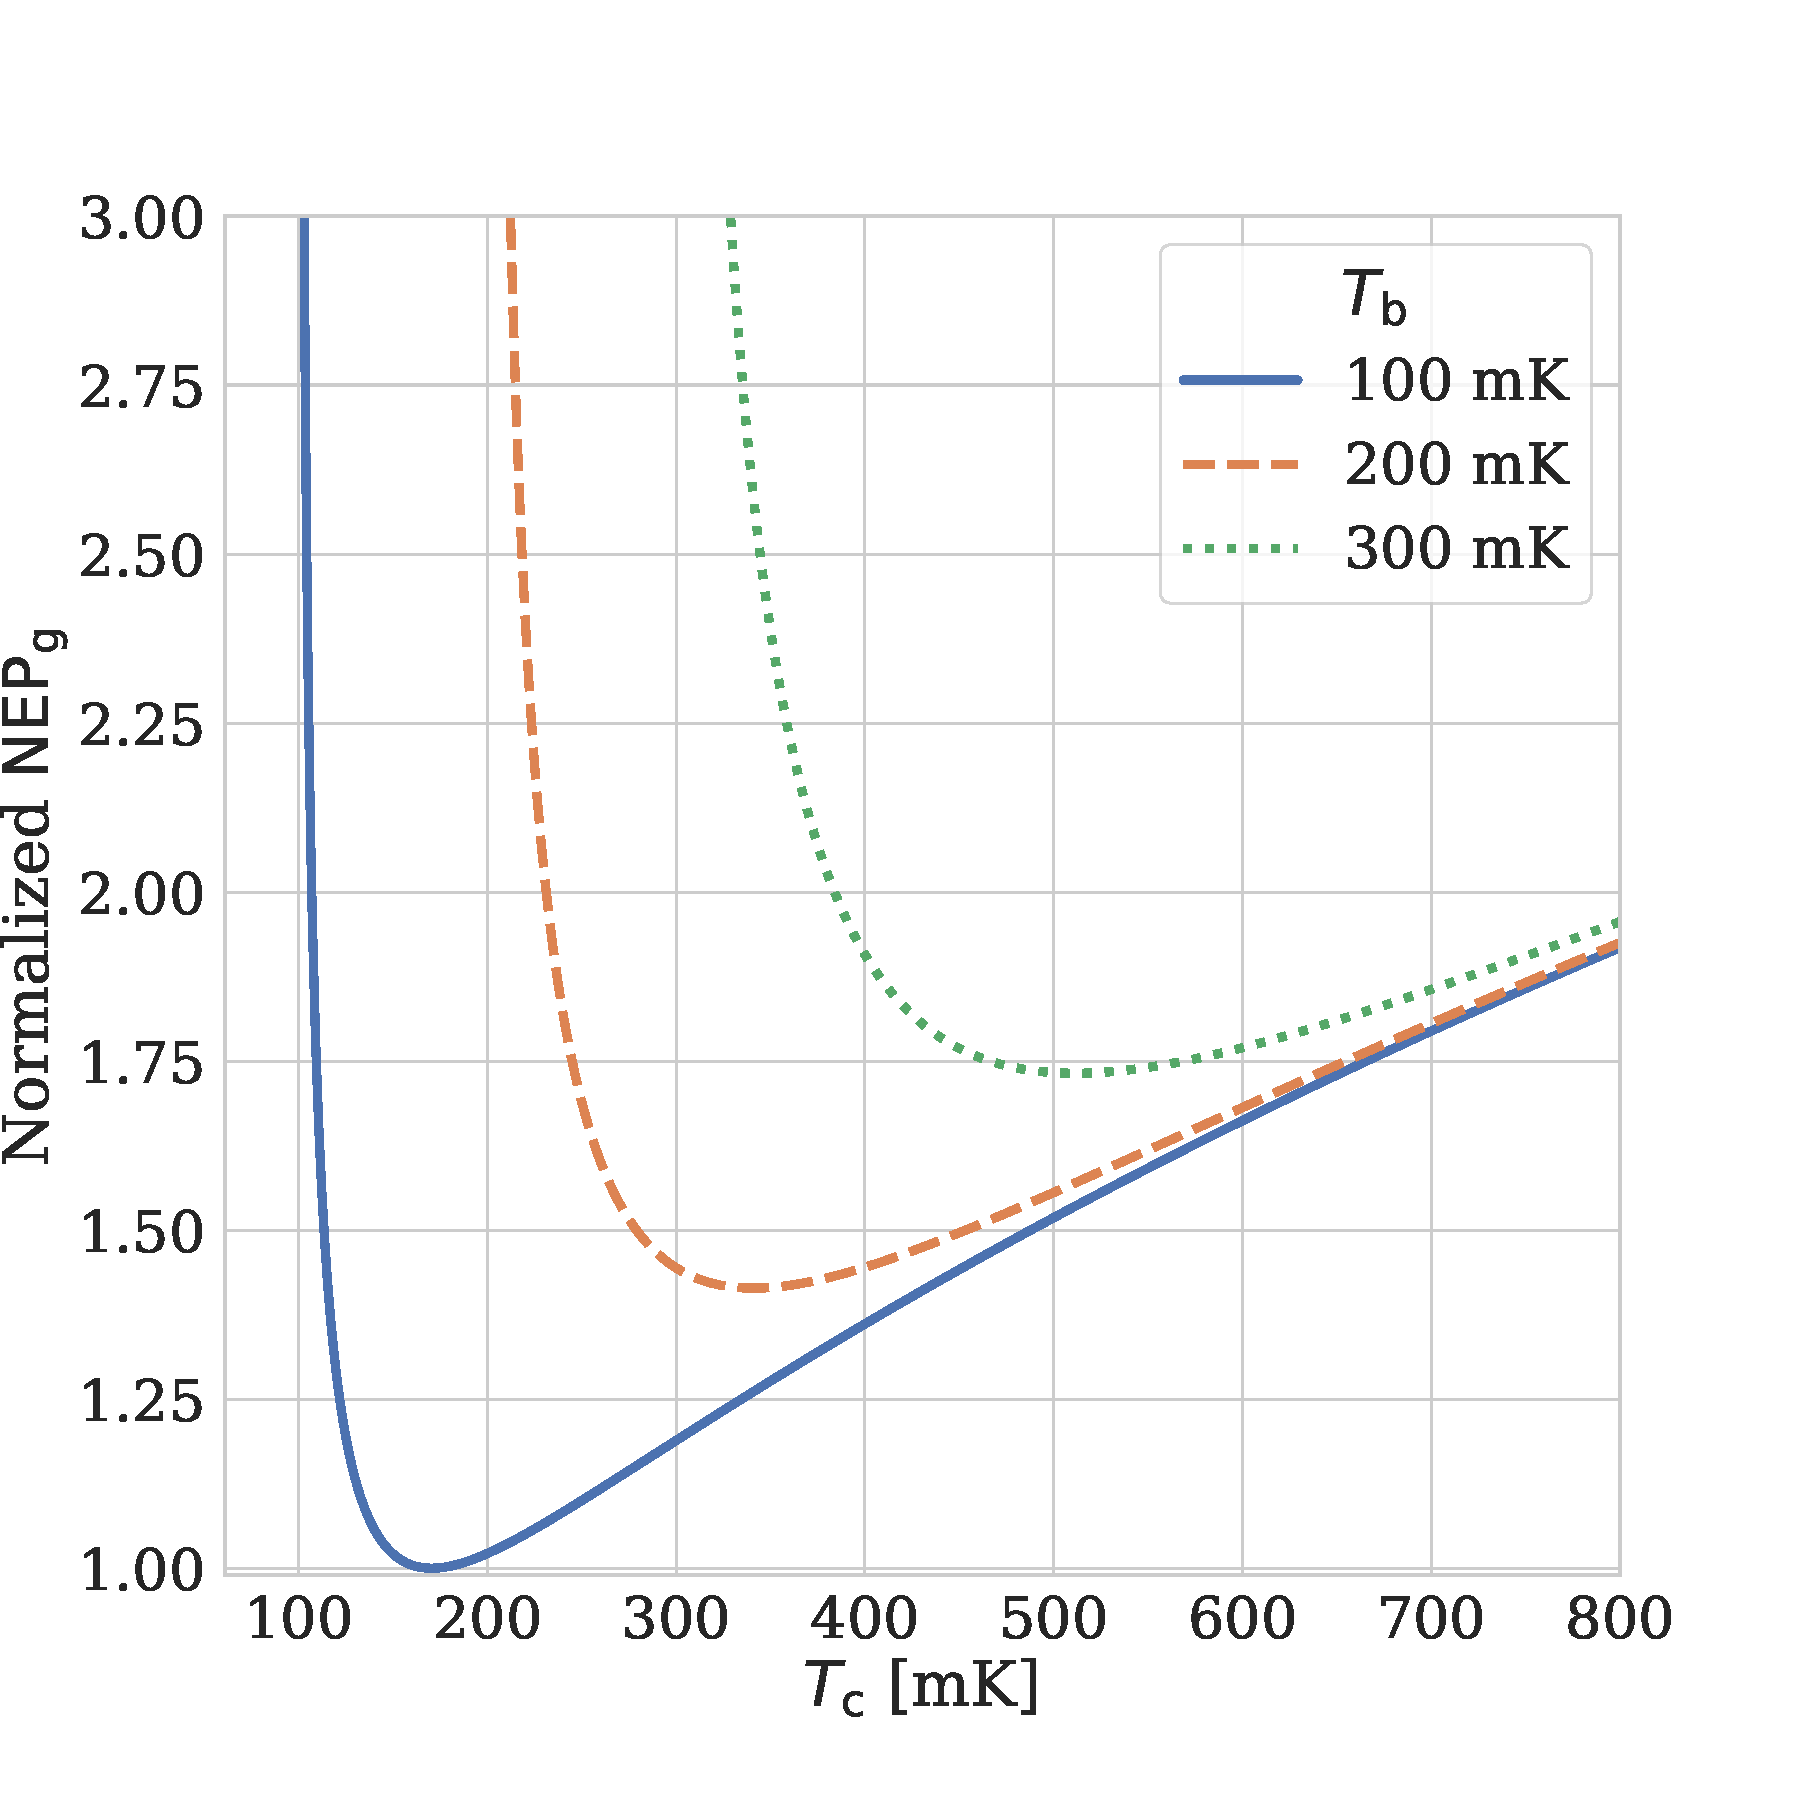
\includegraphics[width=0.48\linewidth, trim=0cm 1cm 2cm 3cm, clip]{SensitivityCalculation/Figures/NEPg_vs_Tc.pdf}}
    \subfloat[\label{fig:nepg_vs_Tc:b}]{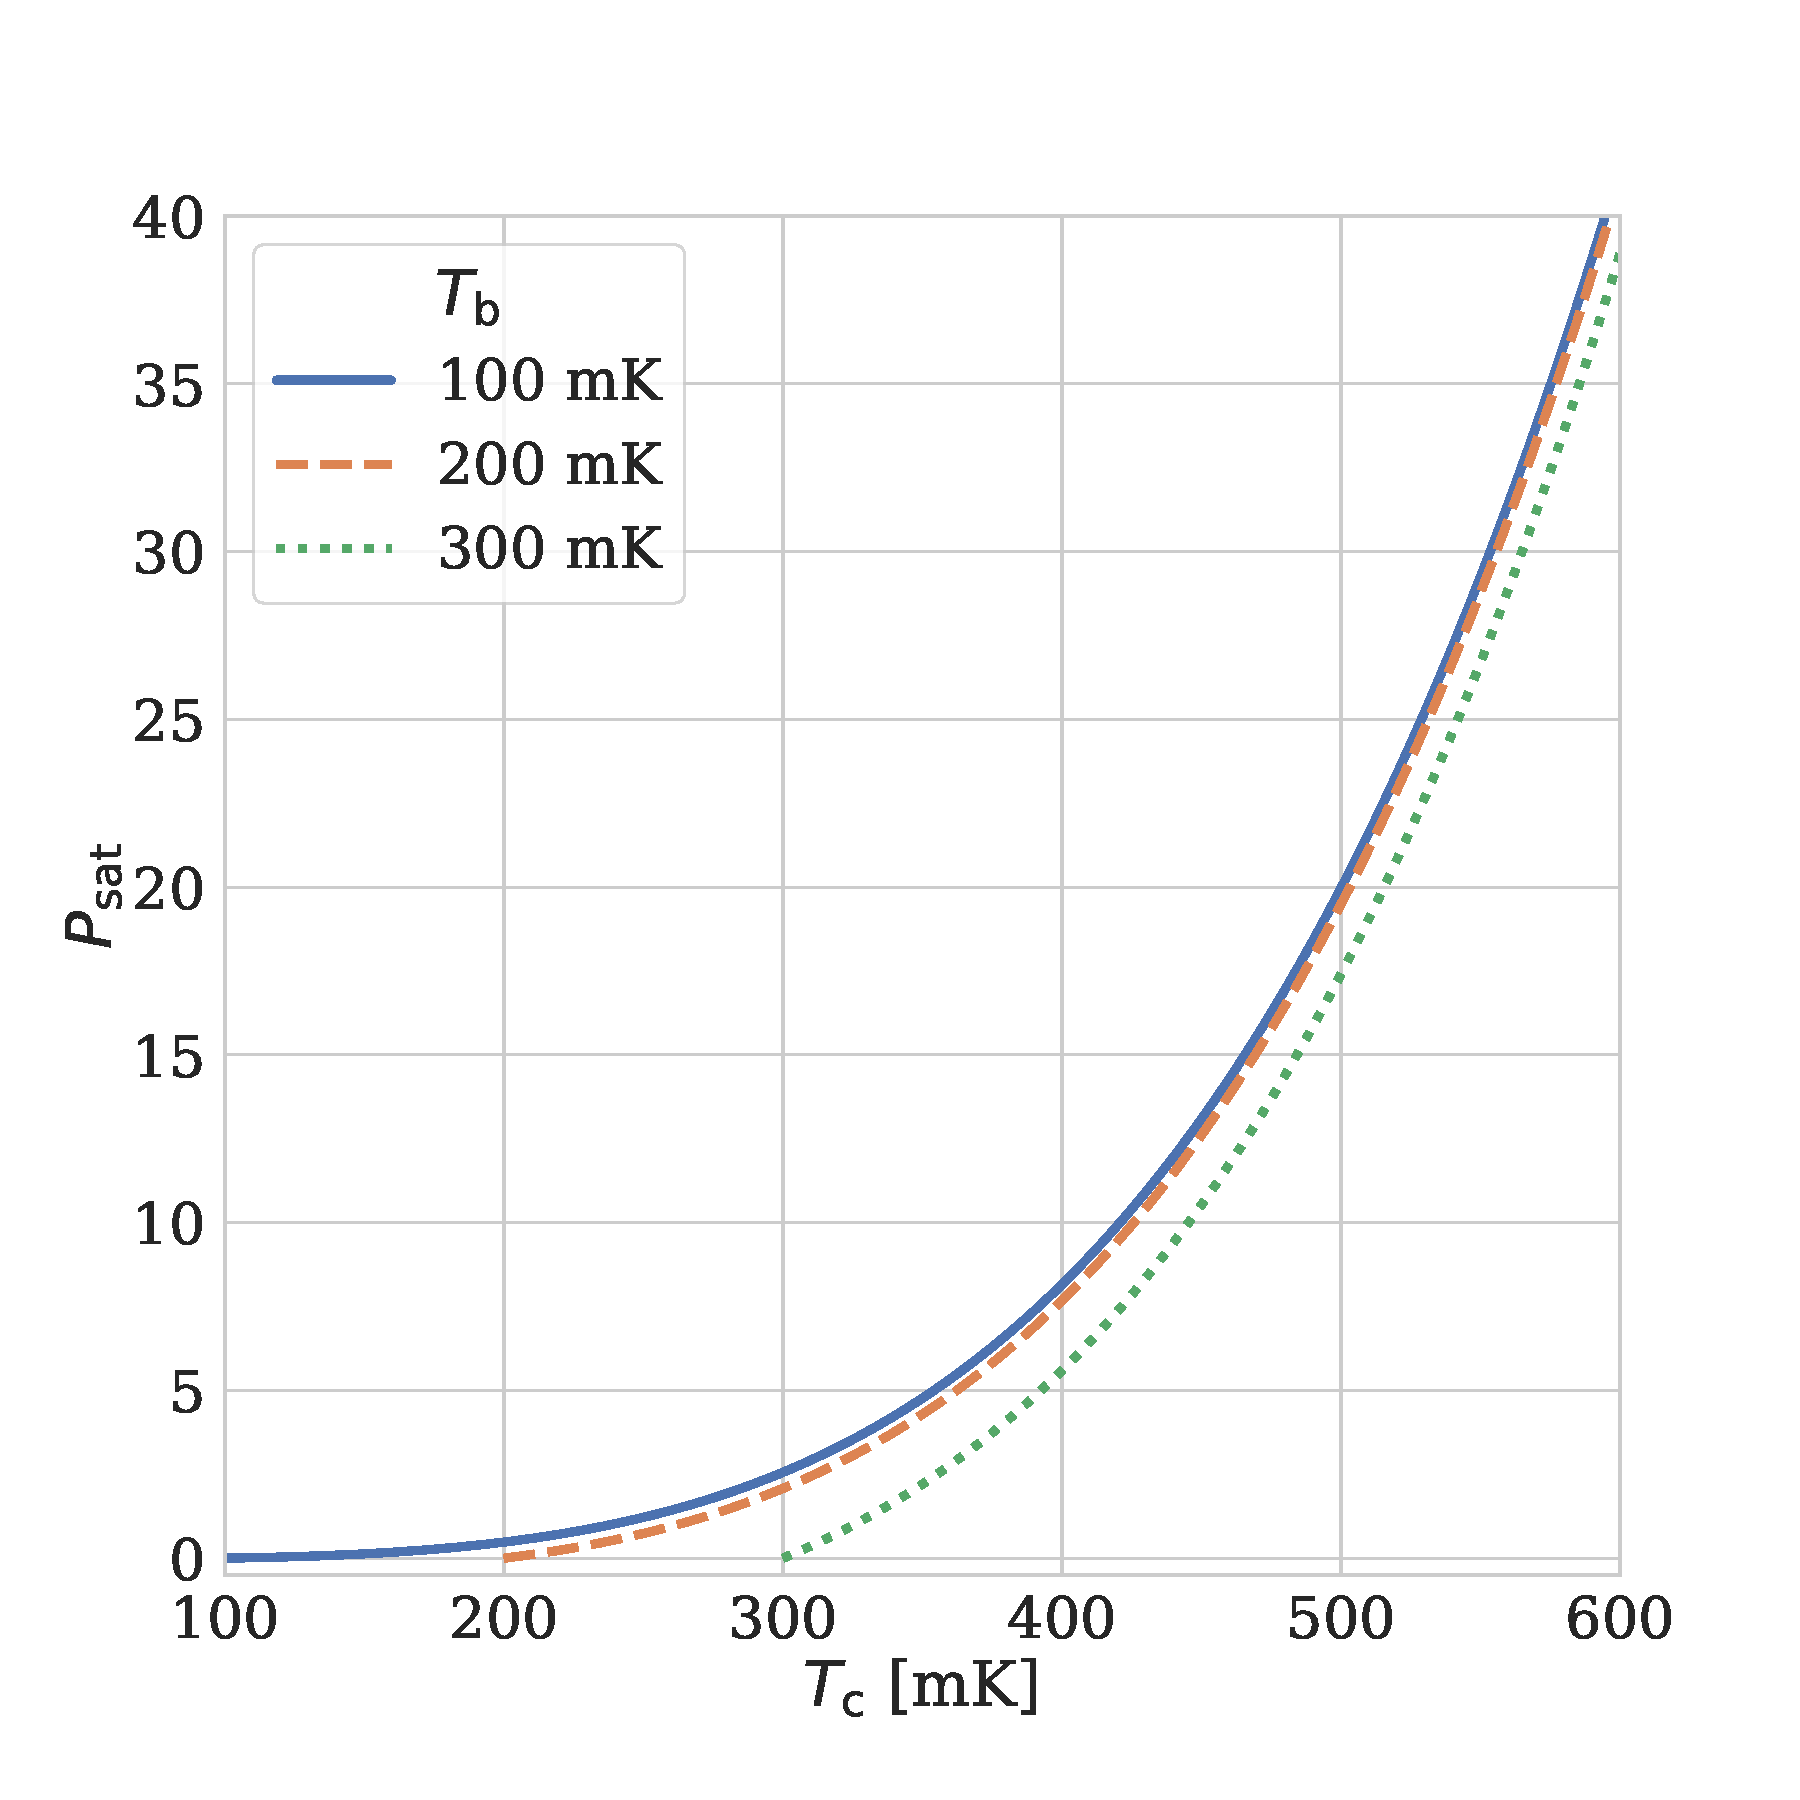
\includegraphics[width=0.48\linewidth, trim=0cm 1cm 2cm 3cm, clip]{SensitivityCalculation/Figures/Psat_vs_Tc.pdf}}
    \caption{Dependence of (a) $\mathrm{NEP_{g}}$ and (b) $P_{\mathrm{sat}}$ on bolometer transition temperature $T_{\mathrm{c}}$ for various bath temperatures $T_{\mathrm{b}}$. (a) assumes a constant $P_{\mathrm{sat}}$, and (b) assumes $A k_{0} / (n + 1) = 240$~$\mathrm{pW / mm \; K^{4}}$ and a bolometer ``leg'' length of 1~mm. Reducing bath temperature substantially improves thermal carrier noise while having little impact on saturation power. For a given $T_{\mathrm{b}}$, there optimum transition temperature is $T_{\mathrm{c}} \approx 1.7 T_{\mathrm{b}}$.}
    \label{fig:nepg_vs_Tc}
\end{figure}

The power flowing from the bolometer to the thermal bath is given by
\begin{equation}
    P_{\mathrm{sat}} = \int_{T_{\mathrm{b}}}^{T_{\mathrm{c}}} \frac{A}{l} k(T) \dd T = \frac{A}{l} \frac{k_{0}}{(n + 1)} \left( T_{\mathrm{c}}^{n + 1} - T_{\mathrm{b}}^{n + 1} \right)
    \label{eq:saturation_power_conductivity}
\end{equation}
where $A$ and $l$ are the cross sectional area and length, respectively, of the link between the TES and the thermal bath. We can then calculate the dynamic thermal conductance as
\begin{equation}
    g = \frac{\partial P_{\mathrm{sat}}}{\partial T} = \frac{A}{l} k_{0} T_{\mathrm{c}}^{n} \, .
    \label{eq:dynamic_conductance_a_over_l}
\end{equation}
While the details of the bolometer thermal link are familiar to those that design and fabricate bolometers, saturation power is typically what's measured, and therefore it's useful to rewrite $g$ as
\begin{equation}
    g = P_{\mathrm{sat}} (n + 1) \frac{T_{\mathrm{c}}^{n}}{T_{\mathrm{c}}^{n+1} - T_{\mathrm{b}}^{n+1}}
    \label{eq:g}
\end{equation}
Therefore, $NEP_{\mathrm{g}} \propto P_{\mathrm{sat}}$, making the tuning of saturation power important to optimizing detector sensitivity. Plugging this conductance into Equation~\ref{eq:nep_g} gives a more phenomenological form for thermal carrier noise
\begin{equation}
    \mathrm{NEP_{g}} = \sqrt{4 k_{\mathrm{B}} F_{\mathrm{link}} P_{\mathrm{sat}}} \sqrt{\frac{\left(n + 1 \right) T_{\mathrm{c}}^{n + 2}}{T_{c}^{n+1} - T_{\mathrm{b}}^{n + 1}}} \, .
    \label{eq:nep_g_phenomenological}
\end{equation}
While Equation~\ref{eq:nep_g_phenomenological} is fully determined by a relatively small set of measurable quantities, in reality $NEP_{\mathrm{g}}$ can vary depending on the specifics of the bolometer geometry, composition and fabrication. For example, transition-edge sensors (TES) have known pathological noise sources, such as flux flow noise and non-equilibrium Johnson noise, that increase the measured $NEP_{\mathrm{g}}$ beyond that of the theoretical presented here. Therefore, $F_{\mathrm{link}}$ is often determined empirically during non-optical characterization both in the lab.

%%%%%%%%%%%%%%%%%%%%%%%%%%%%%%%%
%%%%%%%%%%%%%%%%%%%%%%%%%%%%%%%%
%%%%%%%%%%%%%%%%%%%%%%%%%%%%%%%%

\section{Readout NEP}
\label{sec:sensitivity_readout_noise}

As presented in Section~\ref{sec:simons_array_detectors}, modern CMB detectors are low-impedance, voltage-biased bolometers read out using superconducting quantum interference device (SQUID) transimpedance amplifiers. SQUIDs are current sensors, and a modulation of power on a voltage-biased bolometer corresponds to a modulation of current at the amplifier input. Therefore, SQUID amplifier noise is typically characterized in terms of a noise-equivalent current NEI, which has units of $\mathrm{A /\sqrt{Hz}}$. In order to refer NEI to an NEP, we need to consider the bolometer responsivity $S_{\mathrm{I}} = \mathrm{d} I / \mathrm{d} P$. One useful way to quantify responsivity is via the relation
\begin{equation}
    S_{\mathrm{I}} = -S_{\mathrm{fact}} \frac{1}{V_{\mathrm{elec}}}
    \label{eq:approx_responsivity}
\end{equation}
where $V_{\mathrm{bias}}$ is the bias voltage across the bolometer. In the presence of electrothermal feedback, the bolometer responsivity can typically be written in terms of the bolometer DC loop gain $\mathcal{L}$, the bolometer time constant $\tau$, and the modulation mode frequency $\omega$ as
\begin{equation}
    S_{\mathrm{fact}} = -\tilde{S}_{\mathrm{fact}} \frac{\mathcal{L}}{\mathcal{L} + 1} \frac{1}{1 + i \omega \tau}
    \label{eq:responsivity}
\end{equation}
where $\tilde{S}_{\mathrm{fact}}$ is 1 if $V_{\mathrm{bias}}$ is DC (e.g. time-division multiplexing or microwave multiplexing) or $\sqrt{2}$ if it is AC (frequency-domain multiplexing), as shown in Equation~\ref{eq:readout_responsivity}.

Characterization of the bolometer loop gain $\mathcal{L}$ and time constant $\tau$ are hugely important to determining detector responsivity and hence to correctly calibrating sky power in Watts to amplifier output in ADC counts. As a result, detector responsivity is calibrated frequently in the field using both celestial sources and instrumental techniques. Given an accurate estimate of $S_{\mathrm{fact}}$, \important{readout NEP} can be written as
\begin{equation}
    \mathrm{NEP}_{\mathrm{read}} = \frac{\mathrm{NEI}}{S_{\mathrm{I}}} = \frac{\sqrt{R_{\mathrm{bolo}} P_{\mathrm{bias}}}}{S_{\mathrm{fact}}} \mathrm{NEI} \, ,
    \label{eq:nep_read}
\end{equation}
where we the RMS voltage bias $V_{\mathrm{bias}} = \sqrt{R_{\mathrm{bolo}} P_{\mathrm{bias}}}$.

Readout noise can in general be a conglomeration of a multitude of noise sources and electrical effects, and therefore readout NEI is not synonymous with SQUID NEI. SQUIDs noise is, in general, quite low $\sim$~5~pA/$\mathrm{\sqrt{Hz}}$, while noise in dfMUX systems (which are used by SA) can range anywhere from 10~$\sim$~50~pA/$\mathrm{\sqrt{Hz}}$ and noise in $\mu$MUX systems (which are used by SO) can be even higher. An effective technique to suppress the conversion of these noise sources to power is to minimize $R_{\mathrm{bolo}}$. SO bolometers are DC biased and have a resistance of $\mathcal{O}(10)$~$\mathrm{m \Omega}$, while SA bolometers are AC biased, necessitating a larger resistance to minimize the impact of parasitic series impedances (such as, for example, inductance in the cables and connectors between the SQUID at 4~K and the detectors on mK stage), and have a resistance of $\mathcal{O}(1)$~$\Omega$. Minimizing readout noise a central pursuit of modern experiments, especially as they face the challenges associated with large multiplexing factors at high frequency.

%%%%%%%%%%%%%%%%%%%%%%%%%%%%%%%%
%%%%%%%%%%%%%%%%%%%%%%%%%%%%%%%%
%%%%%%%%%%%%%%%%%%%%%%%%%%%%%%%%

\section{Johnson NEP}
\label{sec:johnson_noise}

Johnson noise arises due to thermal fluctuations in the bolometer which in turn cause resistance fluctuations. Johnson noise equivalent current $\mathrm{NEI}_{\mathrm{johnson}}$ is given by
\begin{equation}
    \mathrm{NEI}_{\mathrm{johnson}} = \frac{1}{\mathcal{L}} \sqrt{\frac{4 k_{\mathrm{B}} T_{\mathrm{c}}}{R_{\mathrm{bolo}}}} \, ,
    \label{eq:nei_johnson}
\end{equation}
where again, $T_{\mathrm{c}}$ the bolometer's operating temperature and $R_{\mathrm{bolo}}$ is its operating resistance. Johnson current noise can be converted to an NEP using the bolometer responsivity $S_{\mathrm{I}}$, which is defined in Equation \ref{eq:responsivity} as
\begin{equation}
    \mathrm{NEP}_{\mathrm{johnson}} = \frac{\mathrm{NEI}_{\mathrm{johnson}}}{S_{\mathrm{I}}} = \tilde{S}_{\mathrm{fact}} \frac{\mathcal{L} + 1}{\mathcal{L}^{2}} \left( 1 + i \omega \tau \right) \sqrt{4 k_{\mathrm{B}} T_{\mathrm{c}} P_{\mathrm{bias}}} \:,
    \label{eq:nep_johnson}
\end{equation}
where $P_{\mathrm{bias}}$ is defined in Equation \ref{eq:p_elec}. 

Two important notes regarding Equation~\ref{eq:nep_johnson}. First, in the limit of large loop gain $\mathcal{L} \gg 1$, which is often achievable for TES bolometers due to their large $\dd R / \dd T$, $NEP_{\mathrm{johnson}} \rightarrow 0$. Second, Johnson noise is suppressed by a factor of factor of $1 / \mathcal{L}$ with respect to readout noise. For these two reasons, it is often customary to ignore Johnson noise when estimate the NEP of TESes. Even in a worse-possible-case scenario of $\mathcal{L} = 1$, the estimated $\mathrm{NEI_{Johnson}}$ for SA (SO) bolometer is $\sim$~5~(20)~$\mathrm{pA / \sqrt{Hz}}$, which is far below the $\mathrm{NEI_{readout}}$ values discussed in Section~\ref{sec:sensitivity_readout_noise}. This comparison becomes even starker when assuming a healthier, more typical loop gain of, for example, $\mathcal{L}$~$\sim$~10.

%%%%%%%%%%%%%%%%%%%%%%%%%%%%%%%%
%%%%%%%%%%%%%%%%%%%%%%%%%%%%%%%%
%%%%%%%%%%%%%%%%%%%%%%%%%%%%%%%%

\section{NET}
\label{sec:sensitivity_calculation_net}

Assuming that the all detector noise sources are white and uncorrelated, the total detector NEP is given as
\begin{equation}
    \mathrm{NEP}_{\mathrm{det}} = \sqrt{\mathrm{NEP}_{\mathrm{ph}}^{2} + \mathrm{NEP}_{\mathrm{g}}^{2} + \mathrm{NEP}_{\mathrm{read}}^{2}}
    \label{eq:nep_det}
\end{equation}
where $\mathrm{NEP}_{\mathrm{ph}}$ is the photon NEP, $\mathrm{NEP}_{\mathrm{g}}$ is the thermal carrier NEP, and $\mathrm{NEP}_{\mathrm{read}}$ is the readout NEP.

Because a bolometer is built to measure fluctuations in the incident power due to fluctuations in the sky temperature, it is useful to convert bolometer NEP into a noise-equivalent sky temperature (NET) 
\begin{equation}
    \mathrm{NET}_{\mathrm{det}} = \frac{\mathrm{NEP}_{\mathrm{det}}}{\sqrt{2} \left( \mathrm{d} P / \mathrm{d} T_{\mathrm{sky}} \right)}
    \label{eq:net}
\end{equation}
where the $\sqrt{2}$ arises due to a unit conversion from output bandwidth $1 / \sqrt{\mathrm{Hz}}$ to integration time $\sqrt{s}$.

\begin{figure}[!t]
    \centering
    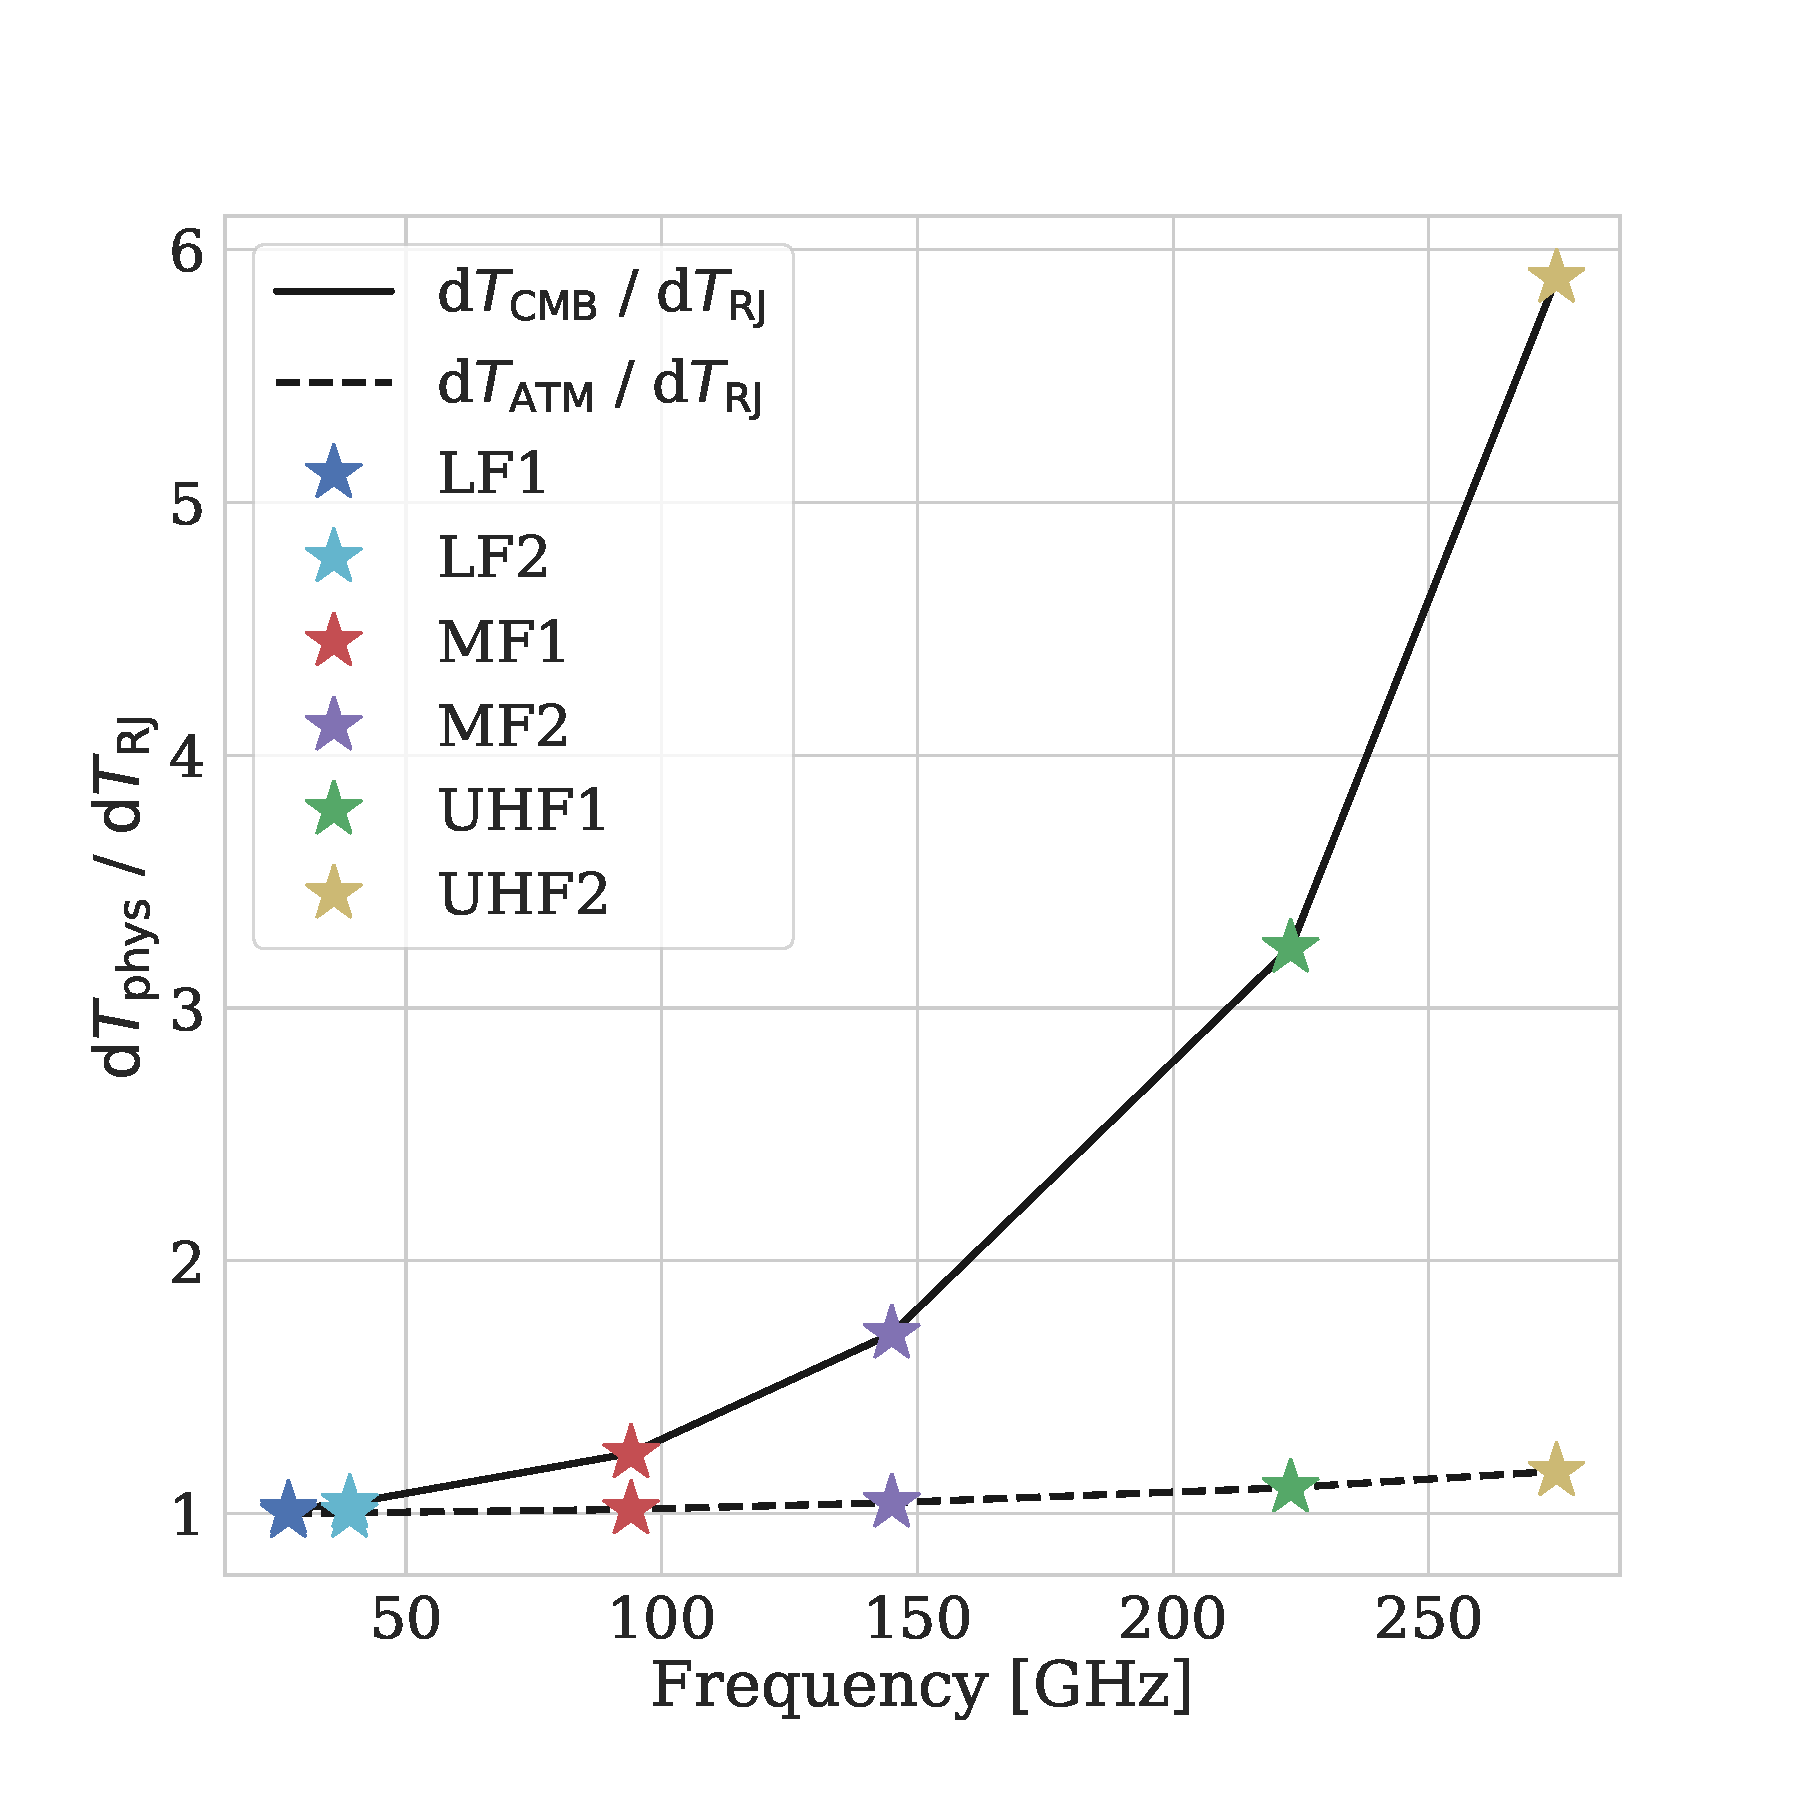
\includegraphics[width=0.6\linewidth, trim=1cm 1cm 1cm 3.5cm, clip]{SensitivityCalculation/Figures/dTcmb_dTrj_conversion.pdf}
    \caption{Conversion factor from RJ temperature fluctuations to that of a blackbody source with temperature $T_{\mathrm{phys}}$. The most commonly used factor is $\dd T_{\mathrm{CMB}} / \dd T_{\mathrm{RJ}}$, which is used to convert $\mathrm{NET_{RJ}}$ to $\mathrm{NET_{CMB}}$, but for reference, the conversion factor for a 10~K atmosphere is also plotted. These lines demonstrate that the Rayleigh-Jeans approximation works well for high temperatures and at low frequencies, and therefore it is often used to assess radio telescopes and IR telescopes that observe bright sources.}
    \label{fig:dTcmb_dTrj}
\end{figure}

CMB experiments often describe sky power referenced to either the CMB with physical temperature $T_{\mathrm{phys}} = T_{\mathrm{CMB}} = 2.725$~K or to some other source with Rayleigh-Jeans temperature $T_{\mathrm{RJ}}$. The conversion factor from fluctuations in the physical temperature of a blackbody with temperature $T_{\mathrm{phys}}$ to power is
\begin{equation}
    \frac{\mathrm{d} P}{\mathrm{d} T_{\mathrm{phys}}} = \xi \int_{0}^{\infty} \left[ \prod_{i=1}^{N_{\mathrm{elem}}} \frac{1}{k_{\mathrm{B}}} \left(  \frac{h \nu}{T_{\mathrm{phys}} \left( \exp \left[ h \nu / k_{\mathrm{B}} T_{\mathrm{phys}} \right] - 1 \right) } \right)^{2} \exp \left[h \nu / k_{\mathrm{B}} T_{\mathrm{phys}} \right] \right] B(\nu) \mathrm{d} \nu
    \label{eq:tcmb_fact}
\end{equation}
where $\xi$ is an overall signal degradation factor, which might be, for example, associated with poor far-field image formation at the focal plane, and $B(\nu)$ is the detector bandpass. The conversion factor for $\mathrm{K_{RJ}}$ is
\begin{equation}
    \frac{\mathrm{d} P}{\mathrm{d} T_{\mathrm{RJ}}} = \xi \int_{0}^{\infty} k_{\mathrm{B}} B(\nu) \mathrm{d} \nu
    \label{eq:trj_fact}
\end{equation}
where $B(\nu)$ is the detector bandpass. Note that Equation~\ref{eq:tcmb_fact} has units of $\mathrm{W / K_{CMB}}$ and that Equation~\ref{eq:trj_fact} has units of $\mathrm{W / K_{RJ}}$.

When reconstructing the sky during analysis, data from each detector are coadded in the map domain to improve signal to noise in the final map. To quantify this SNR increase in the time domain, we defined ``array NET'' as the inverse-variance-weighted average of the NETs of all yielded detectors within a given frequency channel
\begin{equation}
    \mathrm{NET}_{\mathrm{arr}} = \sqrt{\frac{1}{ \sum_{i}^{N_{\mathrm{det}}} 1 /  \mathrm{NET}_{i, \mathrm{det}}^{2}}} \Gamma \, ,
    \label{eq:net_inverse_variance_weight}
\end{equation}
where the sum is over all detectors in the array and where $\Gamma$ is a factor which quantifies the degree to which white noise is correlated between detector pixels on the focal plane (see Section~\ref{sec:sensitivity_calculation_correlation_factor} for more details). 

Equation~\ref{eq:net_inverse_variance_weight} is a useful estimate of aggregate NET as a common technique when combining data (across either multiple detectors or observations) is to weight the data by its inverse variance, to ensure that the highest SNR data is contributing the most power to the combined output. Under a simplifying assumption that all operational detectors have the same $\mathrm{NET_{det}}$, an assumption that is often invoked when forecasting \textit{median} sensitivity estimates, the inverse-variance weighted average becomes the simple average
\begin{equation}
    \mathrm{NET}_{\mathrm{arr}} = \frac{\mathrm{NET}_{\mathrm{det}}}{\sqrt{Y N_{\mathrm{det}}}} \Gamma
    \label{eq:net_arr}
\end{equation}
where $N_{\mathrm{det}}$ is the number of detectors in this frequency channel, $Y$ is the detector yield. Note that nonoperational detectors effectively have infinite $\mathrm{NET_{det}}$.

%%%%%%%%%%%%%%%%%%%%%%%%%%%%%%%%
%%%%%%%%%%%%%%%%%%%%%%%%%%%%%%%%
%%%%%%%%%%%%%%%%%%%%%%%%%%%%%%%%

\section{White-noise correlation factor}
\label{sec:sensitivity_calculation_correlation_factor}

It is possible to oversample the focal plane by deploying more detector pixels than there are non-overlapping spatial modes in the telescope optics. When the pixel density is higher than the mode density, Bose noise correlates between detector outputs. This slows the rate at which noise is averaged down during detector coaddition and is quantified in $\mathrm{NET_{arr}}$ via the factor $\Gamma$ in Equation~\ref{eq:net_arr}. A detailed derivation and discussion of white-noise correlations is discussed in Chapter~\ref{ch:white_noise_correlations}, but we briefly review the calculation here for the completeness of the sensitivity calculation presentation.

The number of optical modes in the telescope is determined by the sky beam size and by the field of view, and it is functionally synonymous with the number of non-overlapping telescope beams. For example, if the telescope's field of view is 5~deg and its beam size is 0.1~deg, the number of independent modes can be approximated as $(5 / 0.1)^{2}$. This description is rough and depends on the details of the beam profile and sidelobes, but this approximation is nonetheless intuitive and functional. In this paradigm, the telescope's magnification determines the linear dimension of the independent modes on the focal plane, which is $\approx 1.2$~$F \lambda$, as shown in Figure~blah. Therefore, if the detectors are packed more closely than $1.2$~$F \lambda$, their noise will start to correlate.

Intensity correlations are determined by the \important{Hanbury Brown-Twiss (HBT) coefficient}
\begin{equation}
    \gamma_{i,j} = \frac{\langle|e_{i}|^{2}|e_{j}|^{2}\rangle - \langle|e_{i}|^{2}\rangle\langle|e_{j}|^{2}\rangle}{\mathrm{RMS}\left(|e_{i}|^{2}\right) \, \mathrm{RMS}\left(|e_{j}|^{2}\right)} \, ,
\end{equation}
where $e_{i}$ is an integral of the electric field over the aperture for detector $i$ with beam $b_{i}(x,y)$ and optical path length to the source $\ell_{i}(x,y)$ 
\begin{equation}
    e_{i} = \iint \mathrm{d}x \, \mathrm{d}y \, e^{2 \pi i \ell_{i}(x,y)} \, b_{i}(x,y) \, E(x,y) \, .
\end{equation}
If the \textit{stop} is not 0~K, correlations can also arise due to radiation outside of the aperture as well. Again, these details are discussed in greater detail in Chapter~\ref{ch:white_noise_correlations}, but for now we focus only radiation within the aperture, which is typically the dominant noise contributor, especially for ground-based telescopes.

\begin{figure}
    \centering
    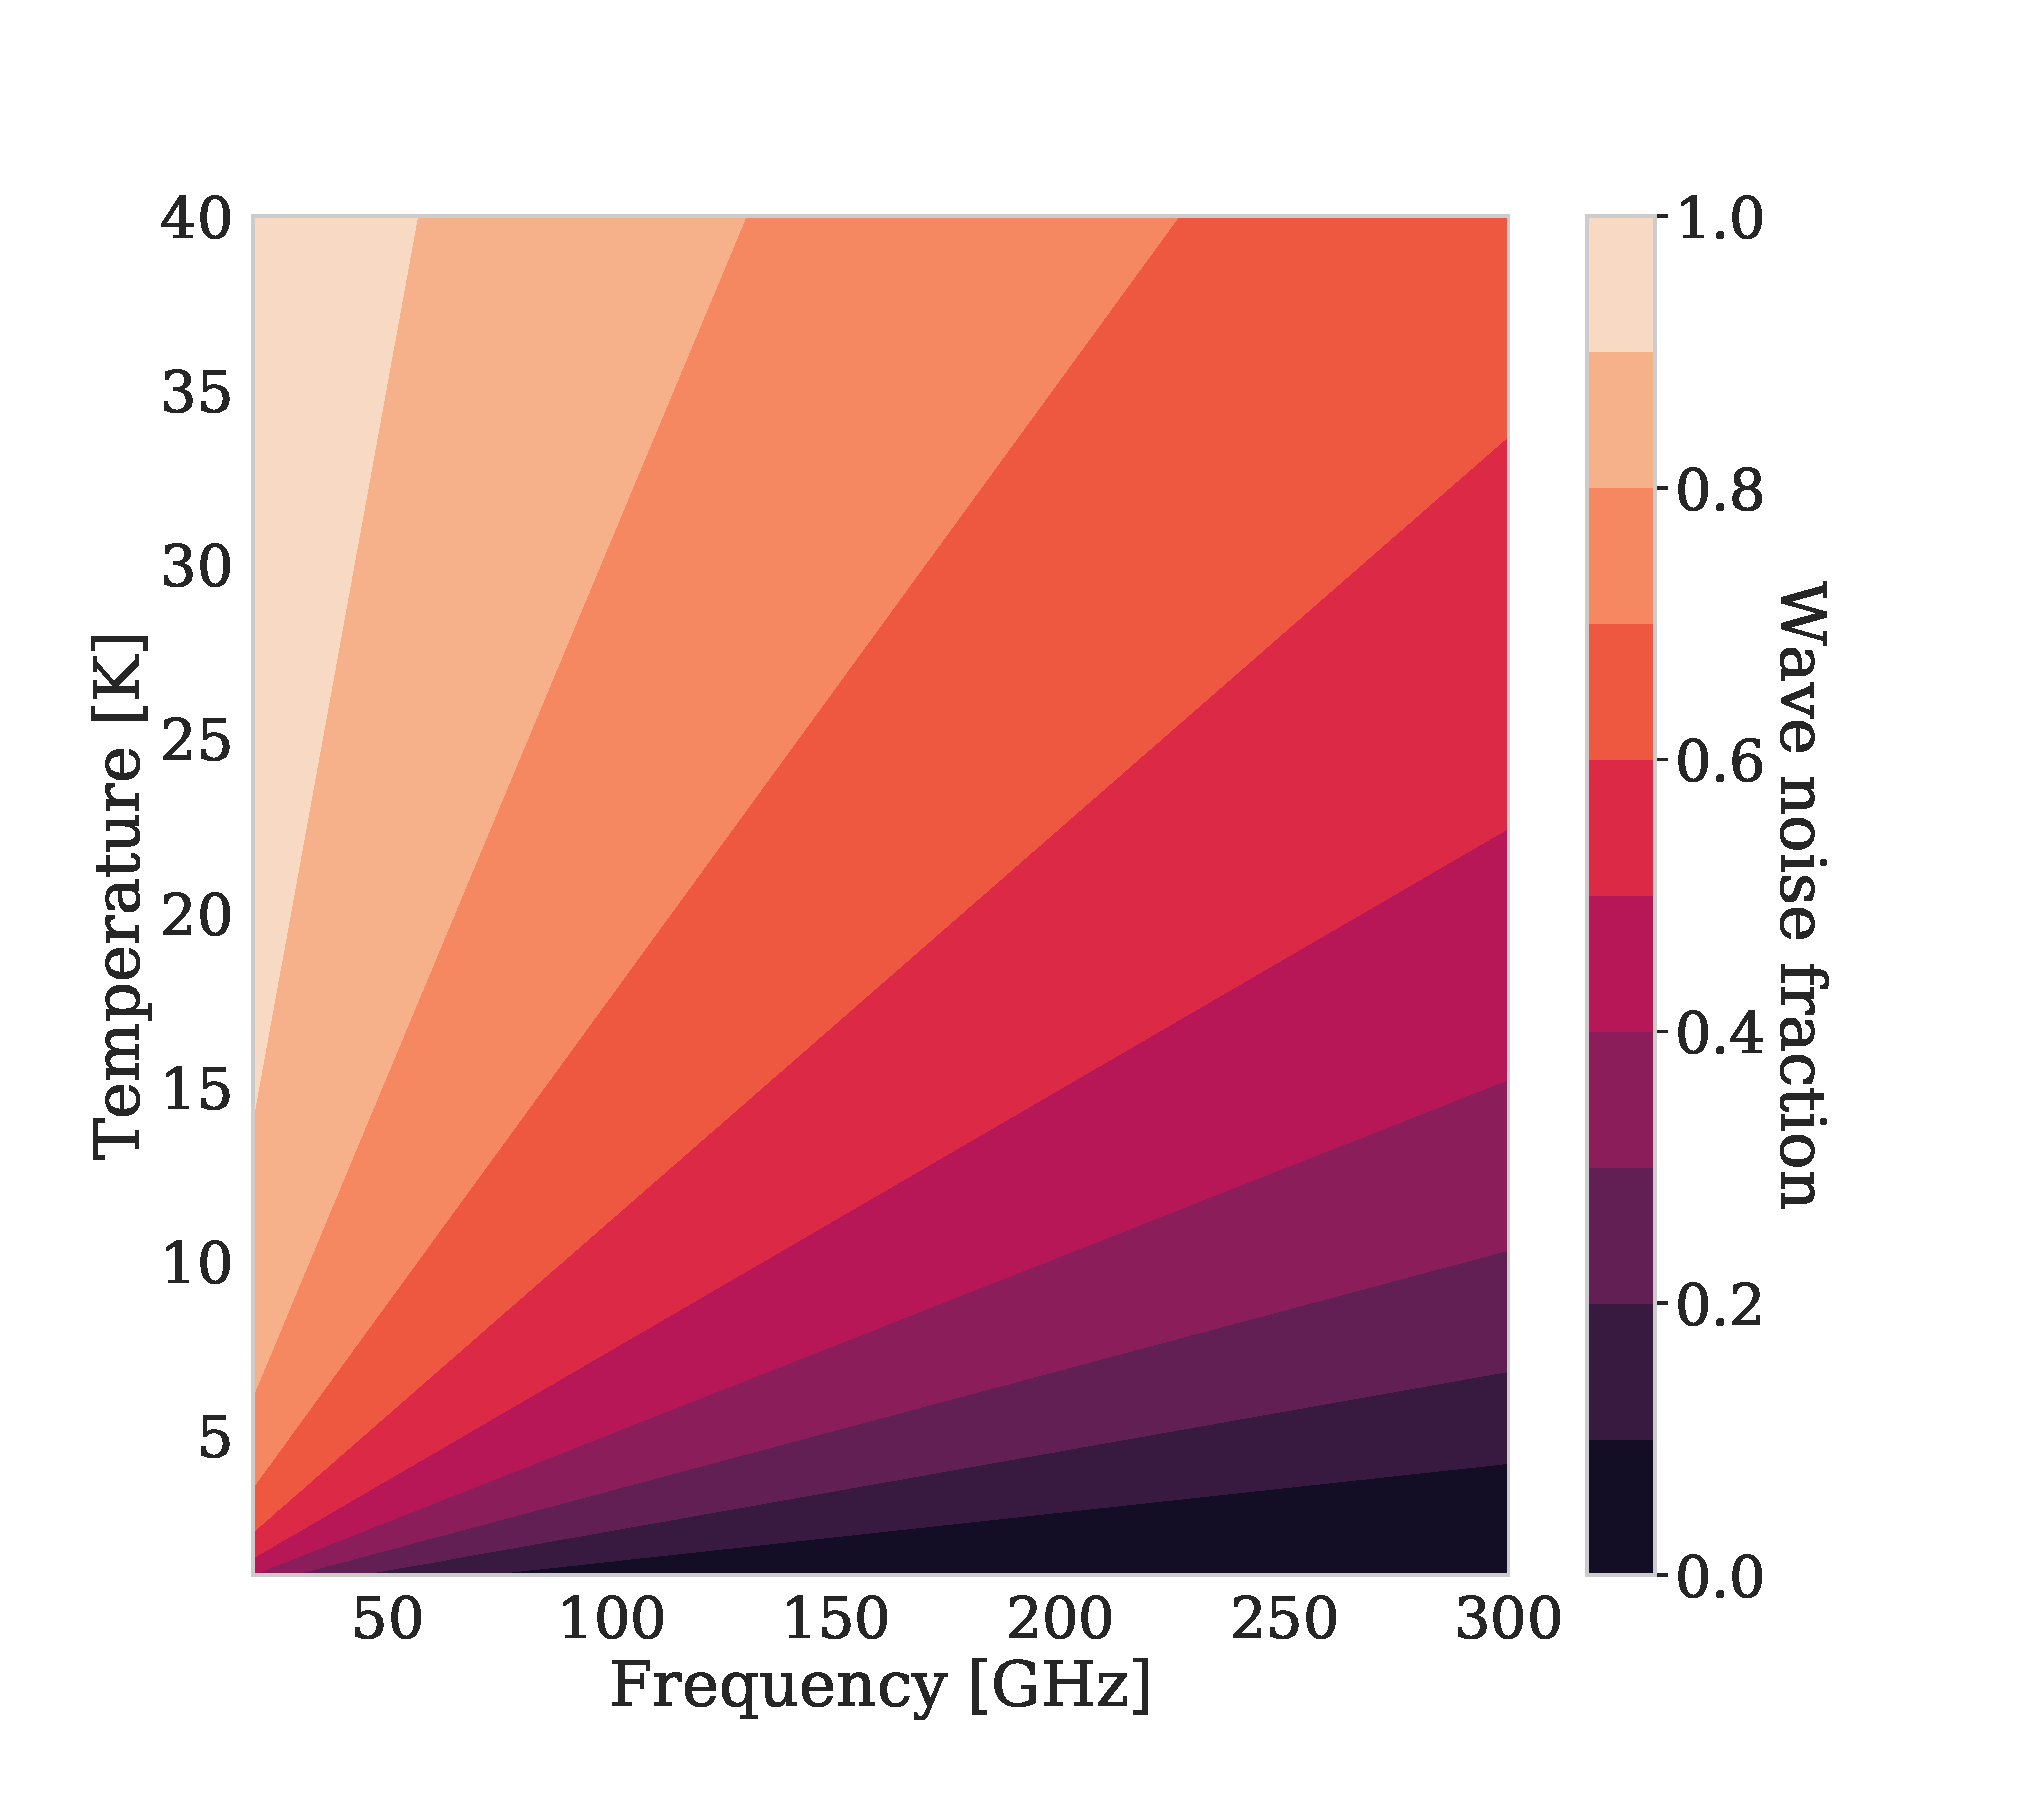
\includegraphics[width=0.65\linewidth, trim=1cm 1cm 1cm 3cm, clip]{SensitivityCalculation/Figures/bose_noise_fraction.pdf}
    \caption{Wave noise fraction, which is defined as $\mathrm{NEP_{wave}} / \sqrt{NEP_{wave}^{2} + NEP_{shot}^{2}}$, assuming a top-hat band of 20~GHz bandwidth and an optical throughput between the source and detector of 30\%.}
    \label{fig:bose_noise_fraction}
\end{figure}

The cumulative correlation coefficient $\gamma$ is given by a summation of the correlation coefficients between all $N_{\mathrm{pix}}$ detector pixels on the focal plane
\begin{equation}
    \gamma = \frac{1}{N_{\mathrm{pix}}-1} \sum_{i} \sum_{j \neq i} \gamma_{i,j}\,\, .
\end{equation}
These correlations then propagate to $\mathrm{NET_{arr}}$ by suppressing the degree to which wave noise is averaged down when inverse-variance averaging the detector data
\begin{equation}
    \mathrm{NET}_{\mathrm{arr}} = \sqrt{\frac{\mathrm{NET}^{2}_{\mathrm{shot}} + (1 + \gamma) \mathrm{NET}^{2}_{\mathrm{wave}} + 
    \mathrm{NET}^{2}_{\mathrm{g}} + \mathrm{NET}^{2}_{\mathrm{read}}}{Y N_{\mathrm{det}}}}\,\, .
\end{equation}
We can now write the array NET correlation suppression factor $\Gamma$ defined in Equation \ref{eq:net_arr} as
\begin{equation}
    \Gamma = \sqrt{1 + \frac{\gamma \, \mathrm{NET}^{2}_{\mathrm{wave}}}{\mathrm{NET}^{2}_{\mathrm{shot}} + \mathrm{NET}^{2}_{\mathrm{wave}} + \mathrm{NET}^{2}_{\mathrm{g}} + 
    \mathrm{NET}^{2}_{\mathrm{read}}}} \; .
    \label{eq:corr_fact}
\end{equation}
As evident in Equation~\ref{eq:corr_fact}, the impact of correlations on array NET depends not only on the the HBT coefficient but on the contribution of wave noise to the total noise in the system and on the optical correlation factor $\gamma$, further emphasizing the importance of an accurate $P_{\mathrm{opt}}$ estimate to an accurate estimate of $\Gamma$.

%%%%%%%%%%%%%%%%%%%%%%%%%%%%%%%%
%%%%%%%%%%%%%%%%%%%%%%%%%%%%%%%%
%%%%%%%%%%%%%%%%%%%%%%%%%%%%%%%%

\section{$N_{\mathrm{\ell}}$ and mapping speed}
\label{sec:N_ell_mapping_speed}

As presented in Section~\ref{sec:sensitivity_calculation_net}, NET has units of $\mathrm{\mu K \sqrt{s}}$ and is a measure noise in the detector time streams referenced to fluctuations in sky temperature. It is often useful to convert this time-domain noise into \important{map depth}, or noise in a sky-map domain, which defined as
\begin{equation}
    \sigma_{\mathrm{map}} = \mathrm{NET}_{\mathrm{arr}} \sqrt{\frac{4 \pi \left( 10,800 / \pi \right)^{2} f_{\mathrm{sky}}}{\eta_{\mathrm{obs}} t_{\mathrm{obs}}}} \, ,
    \label{eq:map_depth}
\end{equation}
in units of $\mathrm{K - arcmin}$. Here, we convert NET from a temporal spectral density to a spatial spectral density by dividing by the square root of \important{integration time}, which is the product of the observatory's lifetime $t_{\mathrm{obs}}$ and its observation efficiency $\eta_{\mathrm{obs}}$, and multiplying by the square root of sky area, which the total number of arcminutes on the sky multiplied the observed sky fraction $f_{\mathrm{sky}}$. In addition to having low NETs, map depth is improved by both integrating for longer and by observing smaller sky patches. However, as shown in Equation~\ref{eq:cosmic_variance}, a smaller sky fraction leads to a larger cosmic variance, and therefore the trade-off between map depth and sky coverage must be carefully considered when optimizing observation strategies to measure large angular scales. 

The figure of merit for power spectrum sensitivity is \important{$N_{\ell}$}, which measures RMS noise in $K^{2}$ in the CMB power spectrum as a function of angular multipole number $\ell$
\begin{equation}
    \Delta C_{\ell} = \sqrt{\frac{2}{\left( 2 \ell + 1 \right) f_{\mathrm{sky}}}} \left( C_{\ell} + N_{\ell} \right) \, ,
    \label{eq:N_ell_in_contex}
\end{equation}
where the first term is the cosmic variance discussed in Section~\ref{sec:cmb_power_spectrum}. $N_{\ell}$ due to white noise can in turn be written using what is often called the \important{Knox Formula}
\begin{equation}
    N_{\ell}^{\mathrm{white}} = 4 \sigma_{\mathrm{map}}^{2} e^{\ell^{2} \sigma_{\mathrm{beam}}^{2}} \, ,
    \label{eq:N_ell}
\end{equation}
where the exponential term is called the \important{beam transfer function} and $\sigma_{\mathrm{beam}}$ is the telescope's angular resolution. The degradation of noise at angular scales smaller than the beam is an important driver of the telescope's primary aperture size. For example, a large-aperture telescope with $\sigma_{\mathrm{beam}} = 0.1$~deg beam will make a much more sensitive measurement of at $\ell = 2,000$ than a small-aperture telescope with $\sigma_{\mathrm{beam}} = 1$~deg, even if the small-aperture telescope has much more sensitive detectors.

\begin{figure}[!t]
    \centering
    \subfloat[\label{fig:noise_curves:a}]{\includegraphics[width=0.48\linewidth, trim=5cm 3.8cm 4.9cm 3.8cm, clip]{SensitivityCalculation/Figures/SO_LAT_TT_noiseCurves.pdf}}
    \subfloat[\label{fig:noise_curves:b}]{\includegraphics[width=0.48\linewidth, trim=5cm 3.8cm 4.9cm 3.8cm, clip]{SensitivityCalculation/Figures/SO_SAT_BB_noiseCurves.pdf}}
    \caption{Forecasted $N_{\ell}$ \important{noise curves} for the SO LAT in temperature and the SO SAT in polarization. The NETs used to formulate these forecasts were calculated using BoloCalc, which is presented in Chapter~\ref{ch:bolocalc}, and the $\ell$ dependencies were found using Equations~\ref{eq:N_ell} and~\ref{eq:N_ell_low_frequency_noise}.}
    \label{fig:N_ell_noise_curves}
\end{figure}

It is important to note that Equations~\ref{eq:map_depth} and ~\ref{eq:N_ell} are crude approximations, and that the conversion from NET to map depth is in general a complicated product of the instrument behavior, observation strategy, and analysis pipeline. For example, telescope scans cover the sky non-uniformly, and the ``weight'' of a given sky pixel is often proportional to its ``hit count,'' or the number of times it was observed, which is in general nontrivial. In addition, time-domain filtering in the detector time streams can lead to sensitivity in the azimuth and elevation (Earth) coordinates differing substantially, and due to a changing sky load with elevation, the depth of a patch in general depends on where in the sky it is scanned. Finally, unlike the assumptions throughout this entire chapter, noise is \textit{not} white but instead increases at low frequencies. The phenomenon is call \important{1/f noise}, and it is typically modeled in $\ell$ space as
\begin{equation}
    N_{\ell} = N_{\ell}^{\mathrm{white}} + N^{\mathrm{red}} \left( \frac{\ell}{\ell_{\mathrm{knee}}} \right)^{\alpha_{\mathrm{knee}}} \, ,
    \label{eq:N_ell_low_frequency_noise}
\end{equation}
where the $\ell$ knee $\ell_{\mathrm{knee}}$, 1/f spectral index
$\alpha_{\mathrm{knee}}$ and 1/f noise amplitude $N^{\mathrm{red}}$ are usually determined empirically.

Noting that the figure of merit for any CMB power spectrum measurement is the noise in power spectrum space, it is quite useful for CMB instrumentalists to quantify instrument sensitivity in terms of \important{mapping speed}
\begin{equation}
    \mathrm{MS} \equiv \frac{1}{\mathrm{NET_{arr}}^{2}} = \frac{N_{\mathrm{det}} Y}{\mathrm{NET_{det}}^{2}} \, .
\end{equation}
Mapping speed quantifies the number of detector-hours needed to reach a specified CMB map depth and is therefore proportional to detector yield observation efficiency. As a result, mapping speed (or mapping speed per cost) is often used as figure of merit during experiment design and optimization.

%%%%%%%%%%%%%%%%%%%%%%%%%%%%%%%%
%%%%%%%%%%%%%%%%%%%%%%%%%%%%%%%%
%%%%%%%%%%%%%%%%%%%%%%%%%%%%%%%%

\section{Discussion}
\label{sec:sensitivity_discussion}
\chapter{White noise correlations}
\label{ch:white_noise_correlations}

Given that the paper is quite pedagogical, I expect this chapter to mimic it closely.
\chapter{BoloCalc: a sensitivity calculator}
\label{ch:bolocalc}

As the CMB field matures, the CMB research field is conglomerating the efforts of many institutions into a smaller number of larger projects. This model allows for larger-budget observatories that can field more detectors and build more complete, self-complimenting telescope designs. There are several challenges associated with coalescing the CMB field into these ``mega experiments,'' and one such logistical challenge is to integrate sensitivity codes into versatile, validated calculator. 

The effectiveness of a sensitivity calculator relies on a few core capabilities:
\medskip
\begin{enumerate}
    \item The code must be \textit{general and modular}, which allows it to simulate a wide variety instrument configurations. This capability is especially important during the early stages of observatory design, when many subsystems are are being optimized in parallel across larger parameter spaces.
    \item The code must be \textit{detailed and comprehensive}, which allows the instrument to be modeled with adequate accuracy. There dozens of inputs to any sensitivity calculation, and while some may be unimportant for one telescope, those same inputs may be hugely important to another. Therefore, it's important that the calculator be able to handle a wide variety of inputs. This capability is especially important during detailed instrument modeling, which can be compared to instrument measurements both in the lab or in the field.
    \item The code must be \textit{easy to use}, which will encourage its use widely throughout the collaboration.
\end{enumerate}
\medskip

With the rise of expansive projects such as Simons Observatory, LiteBIRD, and CMB-S4, so too does the need arise for a sensitivity calculator that can quickly evaluate observatory designs. In addition, with the maturation of SA, there is also a need for detailed sensitivity calculations against which measurements can be compared. In this chapter, we present \important{BoloCalc}, a generalized sensitivity calculator for CMB instrument characterization. The tool is publically available and is being actively used not only within the CMB community but also within IR and radio astronomy.

Because the sensitivity calculation is essential, every experiment in the CMB field has had its own sensitivity code, and because the calculation is straightforward, there has not been an effort to conglomerate these codes across collaborations. However, as the CMB field coalesces, the need for a standardized calculator continues to grow, and therefore BoloCalc's mission is to be so general as to meet the needs of past, ongoing, and upcoming experiments. When it was first conceived, BoloCalc was adapted from a MATLAB sensitivity notebook written by Aritoki Suzuki for the design of the POLARBEAR-2 (now PB-2a), and the PB-2 code was in turn adopted from from other codes before it. In this sense, the innovation of BoloCalc is as much logistical as it is fundamental, and its strength lies in its versatility and generality.

%%%%%%%%%%%%%%%%%%%%%%%%%%%%%%%%
%%%%%%%%%%%%%%%%%%%%%%%%%%%%%%%%
%%%%%%%%%%%%%%%%%%%%%%%%%%%%%%%%

\section{Calculator design}
\label{sec:bolocalc_design}

BoloCalc is a Python code that takes (typically) $\mathcal{O}(100)$ of user-defined inputs and calculates the outputs described in Chapter~\ref{ch:cmb_instrument_sensitivity}, including optical power $P_{\mathrm{opt}}$, photon, thermal, and readout NEP, NET, and mapping speed. While it exists as a standalone command-line tool, it also has a PyQt graphical user interface (GUI) which greatly enhances interaction with the input configuration files and adds real-time data visualization for a quicker, more comprehensive assessments of the outputs.

%%%%%%%%%%%%%%%%%%%%%%%%%%%%%%%%
%%%%%%%%%%%%%%%%%%%%%%%%%%%%%%%%

\subsection{Structure}
\label{sec:bolocalc_structure}

BoloCalc has a modular object-oriented structure, which allows for arbitrary mixtures of sites, telescopes, cameras, optics, focal planes, and detectors. A BoloCalc project has the parent-child structure shown in Fig.~\ref{fig:bolocalc_layout} and is built with four layers: experiments, telescopes, cameras, and channels, which are defined in Tab.~\ref{tab:bolocalc_layers}. Each experiment can have an arbitrary set of telescopes (at different sites), each telescope an arbitrary set of cameras, and each camera an arbitrary set of channels. Each layer of a BoloCalc project contains various user-defined parameters, and the inheritance structure follows that of parent-child such that each telescope inherits the parameters of its experiment, each camera inherits that of its telescope, and each channel that of its camera. This flexible inheritance structure has proven valuable to the designs of SO and LB, especially during their early stages when the number of telescopes, cameras, frequencies, and detectors were undecided and when rapid feedback was needed to evaluate various instrument configurations.

\begin{figure}[ht!]
    \centering
    \includegraphics[width=0.98\linewidth]{BoloCalc/Figures/OrgDiagram.pdf}
    \caption[Generic layout of a BoloCalc project]{Generic layout of a BoloCalc project. There are four layers to a project, each with its own set of parameters: (1) experiments, (2) telescopes, (3) cameras, and (4) channels.  There can be an arbitrary set of $N$ telescopes in each experiment, an arbitrary set of $M$ cameras in each telescope, and an arbitrary set of $P$ channels in each camera. Each telescope inherits the parameters of its parent experiment, each camera inherits that of its telescope, and each channel that of its camera. The black bullet points highlight some important parameter definitions that occur within each layer.}
    \label{fig:bolocalc_layout}
\end{figure}

\begin{table}[!ht]
	\centering
    \tabulinesep=0.8mm
	\begin{tabu}[t]{|| l | p{13cm} ||}
    \hline
    \textbf{Layer} & \textbf{Definition} \\
    \hline
    \hline
    Experiment & An assemblage of CMB telescopes. \\
    \hline
    Telescope & A platform that carries and points one or more cameras. It observes at a specified site with a specified observation strategy and can include warm reflectors. \\
    \hline
    Camera & A cryostat that houses cryogenic optics, filters, and detectors. Multiple cameras can be mounted on the same telescope. \\
    \hline
    Channel & A frequency band observed by some set of detectors within a camera. A multichroic camera will have multiple channels. \\
    \hline
    \end{tabu}
    \caption{Definitions of the layers used to build a BoloCalc project.  \label{tab:bolocalc_layers}} 
\end{table}

Table~\ref{table:telescope} shows the user-defined parameters for Layers 1--4 of a BoloCalc project. Layer 1 defines the foreground parameters for each experiment, which determines the celestial optical loading on the detector. While foregrounds contribute little in-band power relative to the atmosphere and CMB at $\sim$~100~GHz, they can become important to an accurate $P_{\mathrm{opt}}$ estimate for satellite experiments that observe at very high and/or low frequencies and therefore are included in BoloCalc for LB and similar missions \cite{litebird_spie_2018}. Layer 2 defines each telescope's atmospheric conditions, as well as its elevation distribution, observation time and efficiency, and sky fraction. Layer 3 defines each camera's optical chain and magnification, as well as its FOV and focal plane temperature. Layer 4 defines the channels within each camera, including the detector parameters, bandpasses, and antenna beam properties. This layered organization allows BoloCalc to seamlessly interface with the Experiment directory structure, which is shown in Figure~blah. 

The BoloCalc source code is composed of 30 classes which form a tree of inheritance with functional branches. Each of these classes serve a very specific function that when instantiated forms an efficient structure which is important for minimizing computation time. Computational efficiency is especially important when running Monte Carlo realizations of the experiment and when running parameter sweeps, which we describe in detail in the sections that follow.

%%%%%%%%%%%%%%%%%%%%%%%%%%%%%%%%
%%%%%%%%%%%%%%%%%%%%%%%%%%%%%%%%

\subsection{Input and output parameters}
\label{sec:bolocalc_input_parameters}

BoloCalc accepts 65 unique input parameters that are used to define all four experiment levels. The parameters are used to describe the foreground emission, the atmosphere and observation strategy, the camera optics, and the detector specifications. These together are used to generate an instrument model that is then simulated to generate the outputs, which are discussed in Section~\ref{sec:bolocalc_output_parameters}. Below is a list of the inputs, organized by level, along with their corresponding symbol in Section~\ref{ch:cmb_instrument_sensitivity}, which describes the sensitivity calculation.  

\noindent
\important{Level 1 parameters}, common to all telescopes in a given experiment:
\begin{itemize}
    \item Foregrounds
        \begin{itemize}
        \item Dust Temperature: $T_{d}$ in Equation~\ref{eq:dust}
        \item Dust Spectral Index: $n_{d}$ in Equation~\ref{eq:dust}
        \item Dust Amplitude: $A_{d}$ in Equation~\ref{eq:dust}
        \item Dust Scale Frequency: $\nu_{d}$ in Equation~\ref{eq:dust}
        \item Synchrotron Spectral Index: $n_{s}$ in Equation~\ref{eq:synch}
        \item Synchrotron Amplitude: $T_{s}$ in Equation \ref{eq:synch}
        \item Synchrotron Scale Frequency: $\nu_{s}$ in Equation~\ref{eq:synch}
        \end{itemize}
\end{itemize}

\noindent
\important{Level 2 parameters}, common to all cameras in a given telescope:
\begin{itemize}
    \item Observation parameters
        \begin{itemize}
        \item Sky Temperature: $T$ in Equation~\ref{eq:planck_spec}
        \item Site: site at which the telescope observes (see Section~\ref{sec:bolocalc_atmosphere}
        \item Elevation: telescope boresight elevation above the horizon
        \item PWV: precipitable water vapor (see Section~\ref{sec:bolocalc_atmosphere}
        \item Observation Time: $t_{obs}$ in Equation \ref{eq:map_depth}
        \item Sky Fraction: $f_{sky}$ in Equation~\ref{eq:map_depth}
        \item Observation Efficiency: $\eta_{obs}$ in Equation \ref{eq:map_depth}
        \item NET Margin: factor applied to all NETs within a telescope, which can be treated as contingency
        \end{itemize}
\end{itemize}

\noindent
\important{Level 3 parameters}, common to all channels in a given camera:
\begin{itemize}
    \item Camera parameters
        \begin{itemize}
        \item Boresight Elevation: boresight elevation of the camera with respect to the telescope boresight
        \item Optical Coupling: $\xi$ in Equations~\ref{eq:trj_fact} and~\ref{eq:tcmb_fact}
        \item F Number: $F$ in Equation~\ref{eq:aperture_eff}
        \item Bath Temp: $T_{b}$ in Equations~\ref{eq:nep_g},~\ref{eq:g}, and~\ref{eq:flink}
        \end{itemize}
\end{itemize}

\noindent
\important{Level 4 parameters}, common to all channels in a given camera:
\begin{itemize}
    \item Channel parameters
        \begin{itemize}
        \item Band Center: $\nu_{c}$ in Equation~\ref{eq:top_hat}
        \item Fractional Bandwidth: $f_{BW}$ in Equation~\ref{eq:top_hat}
        \item Pixel Size: $D_{pix}$ in Equation~\ref{eq:aperture_eff}
        \item Number of detectors per wafer
        \item Number of wafers per optics tube
        \item Number of optics tubes in this camera
        \item Waist Factor: $w_{f}$ in Equation~\ref{eq:aperture_eff}
        \item Detector optical efficiency: $\eta_{det}$ in Equations~\ref{eq:throughput} and~\ref{eq:band_eff_scale}
        \item Bolometer saturation power: $P_{sat}$ in Equations~\ref{eq:g} and~\ref{eq:nep_read}
        \item Psat Factor: $f_{psat}$ in Equation~\ref{eq:psat_fact}
        \item Carrier Index: $n$ in Equations~\ref{eq:g} and~\ref{eq:flink}
        \item Bolometer transition temperature: $T_{c}$ in Equations~\ref{eq:g},~\ref{eq:flink}, and~\ref{eq:nep_g}
        \item Tc Fraction: $f_{\mathrm{c}}$ in Equation~\ref{eq:foper}
        \item Thermal link factor: $F_{link}$ in Equations~\ref{eq:flink} and~\ref{eq:nep_g} \item Dynamic thermal conductance: $G$ in Equations~\ref{eq:g} and~\ref{eq:nep_g}
        \item Detector yield: $Y$ in Equation~\ref{eq:net_arr}
        \item Readout noise: NEI in Equation~\ref{eq:nep_read}
        \item Bolometer operating resistance: $R_{\mathrm{bolo}}$ in Equation~\ref{eq:nep_read}
        \item Responsivity factor: $S_{\mathrm{fact}}$ in Equations~\ref{eq:nep_read},~\ref{eq:responsivity}, and~\ref{eq:readout_responsivity}
        \item Readout noise fraction: $\Delta_{\mathrm{read}}$ in Equation~\ref{eq:frac_nep_read}
        \end{itemize}
    \item Optics parameters
        \begin{itemize}
        \item Temperature: $T_{\mathrm{i}}$ in Equation~\ref{eq:pow_spec_density}
        \item Emissivity/absorptivity: $\epsilon_{\mathrm{i}}$ in Equation~\ref{eq:pow_spec_density}
        \item Reflectivity: $r_{\mathrm{i}}$ in Equations~\ref{eq:popt},~\ref{eq:throughput}, and~\ref{eq:efficiency}
        \item Optical thickness: $t_{\mathrm{i}}$ in Equation~\ref{eq:dielectric_absorption}
        \item Refractive index: $n_{\mathrm{i}}$ in Equation~\ref{eq:dielectric_absorption}
        \item Loss Tangent: $\mathrm{tan} \delta_{\mathrm{i}}$ in Equation~\ref{eq:dielectric_absorption}
        \item Conductivity: $\sigma_{c}$ in Equation~\ref{eq:conductor_absorption}
        \item Surface Roughness: $\sigma_{r}$ in Equation~\ref{eq:ruze_scattering}
        \item Scatter fraction: $\delta_{i}$ in Equation~\ref{eq:pow_spec_density}
        \item Scatter temperature: $T_{\delta ; i}$ in Equation~\ref{eq:pow_spec_density}
        \item Spillover fraction: $\beta_{i}$ in Equation~\ref{eq:pow_spec_density}
        \item Spillover Temperature: $T_{\beta ; i}$ in Equation~\ref{eq:pow_spec_density}
        \end{itemize}
\end{itemize}
Some optics channel parameters are functionally redundant, offering the user multiple methods for calculating emissivity, efficiency, and scattering. For example, the absorptivity of a refractive optic can be entered explicitly, or it can be derived using loss tangent, thickness, and dielectric constant. In a similar manner, there are multiple ways to define certain channel parameters. For example, dynamic thermal conductance $g$ can either be defined explicitly or derived from $T_{\mathrm{c}}$, $T_{\mathrm{b}}$, and $n$. As another example, readout noise can either be defined using NEI, $R_{\mathrm{bolo}}$, and $P_{\mathrm{sat}}$ or it can be stated as a fraction of the detector NEP, offering some flexibility about the level of specificity needed to define its contribution. These flexibilities make BoloCalc useful for a wide range of scenarios, all the way from defining high-level specifications upon project conception to evaluating the impact of low-level measurements during instrument commissioning.

BoloCalc uses the presented input parameters and the equations in Chapter~\ref{ch:cmb_instrument_sensitivity} to calculate 12 \important{output parameters}: 
\begin{itemize}
    \item Optical Throughput: $\eta_{\mathrm{inst}}$ in Equation~\ref{eq:throughput}
    \item Optical Power: $P_{\mathrm{opt}}$ in Equation~\ref{eq:popt}
    \item Telescope Temperature: $T_{\mathrm{tel}}$ in Equation~\ref{eq:tel_temp}
    \item Sky Temperature: $T_{\mathrm{sky}}$ in Equation~\ref{eq:sky_temp}
    \item Photon NEP: $NEP_{\mathrm{ph}}$ in Equation~\ref{eq:nep_ph}
    \item Bolometer thermal NEP: $NEP_{\mathrm{g}}$ in Equation~\ref{eq:nep_g}
    \item Readout NEP: $NEP_{\mathrm{read}}$ in Equation~\ref{eq:nep_read}
    \item Detector NEP: $NEP_{\mathrm{det}}$ in Equation~\ref{eq:nep_det}
    \item Detector NET (CMB or RJ): $NET_{\mathrm{det}}$ in Equation~\ref{eq:net}
    \item Array NET (CMB or RJ): $NET_{\mathrm{arr}}$ in Equation~\ref{eq:net_arr}
    \item Correlation Factor: $\Gamma$ in Equation~\ref{eq:corr_fact}
    \item Map Depth: $\sigma_{\mathrm{s}}$ in Equation \ref{eq:map_depth}
\end{itemize}
These parameters are calculated for each channel in each camera, but the NETs, map depths, and mapping speeds are also combined via inverse-variance weighting (see Equation~\ref{eq:net_inverse_variance_weight}) at the telescope and experiment levels to give a an estimated \textit{total} sensitivity of multiple detector arrays across multiple cameras and telescopes. Median values of the given outputs are displayed in text tables, but histograms of the data are also available when running many MC instrument realizations to inspect the shape of the distributions. This capability is important for accurate forecasting, as NET distributions tend to be skewed and therefore poorly described using Gaussian distributions, even if the input distributions are Gaussian. 

In addition to outputting the sensitivity outputs described in Chapter~\ref{ch:cmb_instrument_sensitivity}, BoloCalc generates tables of optical power and optical throughput as a function of location within the camera's optics chain. An example of such a table is shown in Figure~blah. This functionality is quite useful for understanding the propagation of optical power through the telescope system and for identifying which areas of the experiment should receive the most attention when trying to improve $\mathrm{NEP_{ph}}$.

%%%%%%%%%%%%%%%%%%%%%%%%%%%%%%%%
%%%%%%%%%%%%%%%%%%%%%%%%%%%%%%%%

\subsection{User interface}
\label{sec:bolocalc_user_interface}

There are two ways to interact with BoloCalc. The first, which has been utilized throughout most of the calculator's lifetime, is through the command line. In this scheme, experiment inputs are set by directly modifying text tables, and outputs are also generated in text tables. There is the a class that loads the outputs in dictionaries, which can in turn be easily unpacked, plotted, and manipulated in a friendly environment, such as that of a Jupyter Notebook. While this first scheme is well-tested and completely self-sufficient, it is cumbersome at times and sets a barrier to entry for new users. Additionally, as is always the case with Python, errors in user inputs are not assessed until execution, and while BoloCalc logging and error tracing is both well developed and comprehensive, the burden of debugging at the command line can be a deterrent for casual users. Therefore, we have also developed a graphical user interface (GUI) using PyQt named \important{BoloCalc GUI} (BCG).

\begin{figure}
    \centering
    \includegraphics[width=0.8\linewidth, trim=6cm 3.4cm 6cm 3.4cm, clip]{PolarizationModulation/Figures/bolocalc_file_structure.pdf}
    \caption{BoloCalc file structure, showing how the file layout mimics the underlying class structure. This layout is modular, making it straightforward to update experiment versions, add telescopes and cameras, and visualize how the various sybsystems fit together.}
    \label{fig:bolocalc_file_layout}
\end{figure}

The GUI substantially improves the BoloCalc user experience in several ways. First, it removes the need for the user to interact with the command line and use text editors. Because BoloCalc has so many inputs, especially those of the optics (described in Section~\ref{sec:sensitivity_optical_power}), text files can be cumbersome to maintain. BCG acts as a wrapper around the input text files, allowing the user to modify parameters using line edits, combo boxes, and check boxes before saving them into the text files. In addition, BCG performs real-time error checking on user input and uses sub windows to control what inputs the user is allowed to enter. This transfers the error checking of inputs to the front end (when they are entered) as opposed to the back end (during Python interpreter operation). In other words, BCG's function to make sure that when the user runs the code, it's guaranteed to work. Second, BCG has embedded descriptions of input and output parameters in said parameter's edit window. This increases the transparency of the sensitivity calculation and provides immediate information about what outputs each parameter influences. While the BoloCalc user manual does lay out the equations in Section~\ref{ch:cmb_instrument_sensitivity} and clearly show which text-file parameter corresponds to which mathematical symbol, it is cumbersome to manage both the manual and the command prompt simultaneously, again acting as a barrier to more casual users. BCG's in-window definitions fix this issue and also act as a pedagogical tool to increase awareness around how the sensitivity calculation works.

\begin{figure}
    \centering
    \subfloat[\label{fig:bcg:a}]{\includegraphics[width=0.8\linewidth, trim=1cm 4cm 1cm 4cm, clip]{BoloCalc/Figures/bcg_optics.pdf}}
    \hfill
    \subfloat[\label{fig:bcg:b}]{\includegraphics[width=0.8\linewidth, trim=2.1cm 3.5cm 1.9cm 3.5cm, clip]{BoloCalc/Figures/bcg_band.pdf}}
    \caption{Two example of the BoloCalc GUI interface. (a) shows the toolbar for navigating between telescopes, cameras, and channels, and it shows a the table interface for editing optical parameters. The drop-down menus allow the values for each channel to be edited independently. (b) shows an example }
    \label{fig:bcg}
\end{figure}

Third, BCG provides real-time data visualization, both of inputs and, after running the code, the outputs. For example, BCG allows the user to view plots of input probability distributions for parameters, as well as bandpass functions for optics and detectors overplotted onto the assumed atmospheric profile. These functionalities provide immediate, informative feedback to the user on the instrument model and allows for rapid assessments of the assumed inputs by collaborators. The outputs can be either downloaded for plot generation by separate scripts, or they can be plotted with somewhat limited options directly in the UI. In a similar way to with the inputs, this allows for a quick assessment of simulation results even facilitates rapid compilation of documentation and presentations. Fourth, BCG effectively separates the BoloCalc code from the user interface, which is enormously useful for development purposes. Any changes in the underlying text files or source code are decoupled from the user, improving backwards compatibility and making the upgrade process more seamless. 

The most important goal of BCG is to make BoloCalc more accessible to wider range of potential users. During instrument design and development, many scientists are evaluating many aspects of a given instrument in parallel, and in the predominant workflow model, if they want feedback on the impact of their measurement on sensitivity, they must go through the collaboration's sensitivity expert, who is typically the one who wrote and manages that collaboration's sensitivity code. This is a barrier-to-entry problem that should be reduced by BCG for ongoing and future experiments, such as SO and CMB-S4, and we hope that whenever anyone from an undergrad to a principal investigator wonders how parameter X impacts output Y, they can quickly use BoloCalc via BCG to assess their curiosity.


%%%%%%%%%%%%%%%%%%%%%%%%%%%%%%%%
%%%%%%%%%%%%%%%%%%%%%%%%%%%%%%%%
%%%%%%%%%%%%%%%%%%%%%%%%%%%%%%%%

\section{Calculator features}
\label{sec:bolocalc_features}

BoloCalc has several features that distinguish it from its predecessor sensitivity codes. A strength of BoloCalc's object-oriented structure is that it is easy to upgrade and modify, and therefore many of the following subsections are the result of collaboration needs that have arisen throughout BoloCalc's lifetime.

%%%%%%%%%%%%%%%%%%%%%%%%%%%%%%%%
%%%%%%%%%%%%%%%%%%%%%%%%%%%%%%%%

\subsection{Site and atmosphere}
\label{sec:bolocalc_site_atmosphere}

BoloCalc uses atmosphere transmissivity and temperature vs. frequency when calculating $P_{\mathrm{opt}}$. Such a spectrum is often called an \important{atmospheric profile} and depends on the details of the observation site, including elevation above sea level, weather patterns, and sky access. There are three ways in which the atmosphere can be defined in BoloCalc: a constant temperature and transmissivity vs. frequency, a custom profile, and simulated profile selected via PWV and horizon elevation. In this section, we want to highlight the final method, which typically both most informative and accurate.

BoloCalc uses atmospheric profiles generated using the \important{AM atmospheric simulation code} developed at Harvard. AM is a \ct{C++} command-line tool which takes a configuration file that contains the details of the molecular composition of atmosphere at a given observation site. BoloCalc uses atmospheric profiles for three different observation sites: the Atacama, the South Pole, and the stratosphere, from where balloon-borne experiments typically observe. Atmospheric configurations for BoloCalc were provided by Denis Barkats and Scott Paine, and their mm-wave behavior has been compared to sky-temperature measurements of the South Pole Telescope and the Atacama Cosmology Telescope, showing excellent agreement. 

A side-by-side comparison of the assumed atmospheric configurations are shown in Figure~blah, and there are a few aspects to these files that are worth pointing out. (Talk a bit about the various assumptions and components here).

In order to offer ready access to the atmospheric profiles, BoloCalc includes an HDF5 file containing spectra over [0.1, 0.2, ... 1,000]~GHz for all three sites over a PWV range of [0, 0.1, ..., 8]~mm and over an elevation range of [0, 1, ..., 90]~deg above the horizon. Then, when the user defines the Layer 2 parameters \textit{site}, \textit{elevation}, and \textit{PWV}, BoloCalc accesses the corresponding profile using the Python class \ct{h5py}. The HDF5 construction is ideal for this functionality, as it offers fast look-up access to the atmospheric profiles without having to load them into memory. The quick access becomes even more important when running MC realizaions of the sky (see Section~\ref{sec:bolocalc_monte_carlo}).

Note that BoloCalc does not make any simplifying assumptions about how the atmospheric loading changes with elevation or PWV. However, as Figure~blah shows, the approximations are reasonable at low frequencies and low PWV and elevation. 

%%%%%%%%%%%%%%%%%%%%%%%%%%%%%%%%
%%%%%%%%%%%%%%%%%%%%%%%%%%%%%%%%

\subsection{Monte Carlo simulations}
\label{sec:bolocalc_monte_carlo}

From forecasting an instrument's scientific impact to measuring its performance in the field, there will always be uncertainties surrounding the sensitivity estimate, and quantifying these uncertainties is critical to every stage of the experiment. For example, when iterating on high-level design concepts during early stages, there will naturally be enormous error bars surrounding back-of-the-envelope calculations and crudely modeled simulations, and understanding how these uncertainties propagate to NET can inform how to formulate a proposal with adequate resource allocations, contingency scenarios, and properly calibrated science objectives. As an example on the other end of the spectrum, when using planet observations in the field to characterize the responsivity of the detectors, it is important to quantify measurement uncertainties, variations across the focal plane, and modelling limitations so as to not misinterpret the telescope's capabilities. Given the importance of uncertainty modeling, BoloCalc uses MC simulations of the instrument to generate histograms of output parameters.

BoloCalc accepts either a mean and standard deviation or a custom probability density for every input parameter. For custom spectral bands (see Section~\ref{sec:bolocalc_custom_bands}), every data point can be defined by a mean and standard deviation, and distributions in PWV and elevation correspond to an uncertainty in the atmospheric profile (see Section~\ref{sec:bolocalc_site_atmosphere}). BoloCalc breaks MC simulations into three levels: (1) realizations of the foregrounds, telescope, camera, and optics, (2) realizations of the sky, and (3) realizations of the detector parameters. The number realizations are defined separately for each level, meaning that for each of $N$ experiments, $M$ skies, are generated, and for each of $M$ skies, $P$ detectors are generated. Separating the simulation into these three categories is chronologically intuitive: (1) you build and field a telescope which after deployment is relatively static, and then (2) you observe with that telescope in a variety of sky conditions, and then (3) given the sky conditions, you calibrate detector operating parameters. Perhaps more importantly, this division is computationally efficient, as it allows the layers shown in Figure~\ref{fig:bolocalc_layout}) to be simulated from the top down.

In its current form, BoloCalc does not offer any functionality for defining correlated errors. Doing so in a general way would require the user to interact with a large correlation matrix, which is a substantial development project. Such a capability would be particularly useful for quantities whose fluctuations are obviously correlated, like temperatures of optical elements, which depend on the cryostat performance, or the waist factor of detectors in different channels, which share the same optical coupling element on multichroic detector pixels. To counteract this deficiency, BoloCalc offers a comprehensive parameter sweep functionality, which can be used to calculate input-output covariances manually.

%%%%%%%%%%%%%%%%%%%%%%%%%%%%%%%%
%%%%%%%%%%%%%%%%%%%%%%%%%%%%%%%%

\subsection{Parameter sweeps}
\label{sec:bolocalc_parameter_sweeps}

What most clearly separates BoloCalc from its predecessors is its parameter sweep functionality. When defining instrument specifications, it is critical to understand the derivatives of NET vs. various instrumental performance metrics. The scope of useful parameter-sweep studies is very large, and therefore BoloCalc's functionality is completely general in an effort to handle a wide variety of common inquiries such as NET vs. elevation, photon NEP vs. primary spillover, and readout NEP vs. saturation power.

BoloCalc allows you to simulate any sweep across any set of parameters across any of the channels in the experiment. There is an option to either calculate all possible permutations of the parameter sweeps or to sweep over them together, and the input vector can either be defined with linear spacing or passed via a custom input file. MC simulations can also be carried out for each parameter set, allowing the user to inspect not only how a parameter sweep changes the mean/median NET but also how it might change the shape of its distribution.

Parameter sweeps, especially when combined with MC simulations, can be computationally expensive, and therefore substantial effort has been put towards ensuring that BoloCalc sweeps are performed efficiently. To do this, an ``initial'' experiment realization is constructed, and as each parameter is changed, only the affected instrument aspects are resimulated. For example, if the user changes the detector optical efficiency of a 90~GHz bolometer in Camera~1, only the MC realizations of the 90~GHz detectors in Camera~1 are recalculated, while the the other channels (e.g. 150~GHz), the telescope optics, and all other cameras and telescopes are left untouched. However, if the spillover fraction of the telescope's primary mirror is varied, then all of the cameras and detectors in that telescope are recalculated, while other telescopes are left untouched. This top-down scheme enables for rapid iteration over many parameters on a time scale of minutes, even when simulating thousands of instrument realizations. 

The parameters sweep output files are carefully constructed for friendly inspection, and an \ct{output.py} class loads these files into dictionaries for easy plotting. In addition, BCG contains a comprehensive system of comboboxes that allows the user to plot any output vs. an arbitrary combination of input parameters, enabling even quicker and easier feedback to instrument designers.

%%%%%%%%%%%%%%%%%%%%%%%%%%%%%%%%
%%%%%%%%%%%%%%%%%%%%%%%%%%%%%%%%

\subsection{Custom bandpasses}
\label{sec:bolocalc_custom_bands}

BoloCalc offers two ways to handle \important{bands}, or input parameters that vary with frequency, such as absorptivity, transmissivity, reflectivity, spillover fraction, and scattering fraction. The first method is define a \important{top-hat band}
\begin{equation}
    B ( \nu) = 
    \begin{cases}
        0    & \text{if } \nu < \nu_{\mathrm{lo}} \\
        \alpha(\nu) & \text{if } \nu_{\mathrm{lo}} \leq \nu \leq \nu_{\mathrm{hi}} \\
        0    & \text{if } \nu > \nu_{\mathrm{hi}} \, ,
    \end{cases}
    \label{eq:bolocalc_tophat_band}
\end{equation}
where $\alpha(\nu)$ is, in general, a function of frequency and where the band edges $\nu_{\mathrm{lo}}$ and $\nu_{\mathrm{hi}}$ are defined by discontinuities. The most common top-hat band is when $\alpha(\nu) = \mathrm{const.}$, giving rise to a rectangular window function. The top-hat band definition is convenient because its spectral extent is defined by only band center $\nu_{\mathrm{c}}$ and fractional bandwidth $f_{\mathrm{BW}}$
\begin{align}
    \nu_{\mathrm{lo}} = \nu_{\mathrm{c}} - \frac{ \nu_{\mathrm{c}} \, f_{\mathrm{BW}}}{2} \label{eq:band_lo} \\
    \nu_{\mathrm{hi}} = \nu_{\mathrm{c}} + \frac{ \nu_{\mathrm{c}} \, f_{\mathrm{BW}}}{2} \label{eq:band_hi} \, ,
\end{align}
making the estimate of band-averaged quantities algebraically trivial.

In reality, bands have spectral features that arise due to any number of physical factors. For example, in an optical element, \important{Fabry-Perot} fringes in transmissivity appear due to peaks/troughs of maximum constructive/destructive interference. For another example, ripples develop in detector bands due to internal reflections between on-chip capacitors used to define the band itself. Also, bands in general have a roll-off that is not infinite, and the shape of this roll-off can be important for understanding the impact of, for example, atmospheric lines on $P_{\mathrm{opt}}$. For these reasons and more, BoloCalc accepts custom input bands (in either TXT or CSV format), with both mean parameter value and standard deviation over an array of frequencies. An additional feature is that BoloCalc also allows the band centers of these input bands to be either swept or assigned an uncertainty during MC simulations. Band center uncertainty is a major component of detector fabrication, and therefore this features has proven to be valuable for detector characterization and design feedback.

The frequency resolution of any BoloCalc simulation can be tuned to $\Delta f \geq 0.1$~GHz, offering the user another lever to optimize computation time vs. accuracy. For example, if a lab measurement of an optical element is performed with high frequency resolution, the user can opt to also run the BoloCalc simulation with high frequency resolution to best capture the impact of the optic measurement on NET. In the other limit, if the user is using band with minimal features (such as top-hats) but wants to run hundreds of thousands of simulations to best quantify the influences of measurement uncertainties, they can increase the frequency resolution to maintain a reasonable computation time. 

%%%%%%%%%%%%%%%%%%%%%%%%%%%%%%%%
%%%%%%%%%%%%%%%%%%%%%%%%%%%%%%%%
%%%%%%%%%%%%%%%%%%%%%%%%%%%%%%%%

\section{Calculator validation}
\label{sec:bolocalc_validation}

In 2014, BoloCalc was born to forecast NETs for LiteBIRD in order to inform the design of its detector arrays. In order to ensure its accuracy, the sensitivity code was checked against that of LiteBIRD's Japanese team, and all outputs were confirmed to be identical for a variety of input assumptions. During the same period, several sets of output parameters vs. input parameter sweeps were compared against legacy codes, such as those of POLARBEAR-2 (Aritoki Suzuki) and SPT-SZ (Nils Halverson) to ensure that mapping speed limits and scalings were consistent.

In 2016, during the early stages of SO, BoloCalc was further compared against sensitivity codes from ACT (Suzanne Staggs and Sarah Marie Bruno) to ensure that relative mapping speed scalings were consistent across many different parameters. This comparison was especially critical during this early period of calculating mapping speed vs. cost for a plethora of instrument configurations, some of which are discussed in Section~\ref{sec:bolocalc_informing_so_design}.

Shortly thereafter, as SO's instrument design matured and its science forecast paper was being actively worked on, BoloCalc models were built for POLARBEAR, ACTpol, Advanced ACTpol, and ABS, all of which have published array NETs against which the BoloCalc prediction were compared. This comparison covered a wide variety of frequencies from 30~GHz to 270~GHz and multiple detector, optical, and telescope infrastructures. For each case, the achieved array NET was within $1 \sigma$ of BoloCalc's median expectation, inspiring confidence that the calculator is indeed detailed and accurate enough to predict and characterize actual instrument performance. This final comparison is very important to the validity of the calculator for the broader CMB community, especially CMB-S4, and therefore we plan to publish our findings in an upcoming paper.

%%%%%%%%%%%%%%%%%%%%%%%%%%%%%%%%
%%%%%%%%%%%%%%%%%%%%%%%%%%%%%%%%
%%%%%%%%%%%%%%%%%%%%%%%%%%%%%%%%

\section{Informing the design of SO}
\label{sec:bolocalc_informing_so_design}

One of BoloCalc's primary applications has been to inform the design and development of SO. During SO's earliest stages, there were a menagerie of open questions about the instrument design. In order to make progress, SO needed an efficient feedback loop between the science team---which studies SO science targets and the needed map depths to achieve them---and the instrument team---which translates the science team's recommendations into an observatory concept and assess its technological feasibility and cost. During these early stages, BoloCalc was a crucial ``glue'' that bound these discussions together by calculating the NET of a given instrument design. In this section, we discuss some of BoloCalc's most important SO design studies both to showcase the calculator's utility and to highlight it's contributions to the resulting SO design. 

The SO design is discussed as part of Chapter~\ref{ch:cmb_instrument_overview}, but we review the basics here before diving into details. SO uses dichroic pixels and distributes its frequency bands between 27/39~GHz ``low-frequency'' (LF) pixels, 90/150~GHz ``mid-frequency'' (MF) pixels, and 220/270~GHz ``ultra-high-frequency'' (UHF) pixels. Lenslet-coupled sinuous antennas are baselined for the LF wafers, while a feedhorn and OMT architecture is baselined for the MF and UHF wafers. The wafers are distributed between cameras in the LAT, which each house three wafers\footnote{The LAT cameras have a FOV that can accommodate up to 4~wafers, allowing for future upgrades.}, and the SATs, which each house seven wafers.

%%%%%%%%%%%%%%%%%%%%%%%%%%%%%%%%
%%%%%%%%%%%%%%%%%%%%%%%%%%%%%%%%

\subsection{LATR architecture}
\label{sec:bolocalc_latr_design}

The LAT is the vehicle for SO's high-$\ell$ science, and its goal is to achieve arcminute resolution in 6 frequency bands from 30~GHz to 280~GHz across an 8~deg FOV. In order to achieve this goal, both the telescope and receiver need to be quite large and are therefore huge cost drivers. For this reason, among others, the LAT system was designed top-down, with the telescope design driving that of the LATR, which drove that of the optics tubes, which drove that of the detector arrays. Of course there was iteration and interaction among the teams that designed each subsystem, and the much of the optimization ran both ways, but for the LAT discussions to follow, much of the larger elements are held constant while the smaller elements are optimized.

The LAT has a field of view of $7.8^{\circ}$ that illuminates a 2.5~m diameter area at the telescope's focus. At this point, it is the job of the LATR to reimage the telescope image onto detector arrays. An early application of BoloCalc was to help determine how many optics tubes to deploy in the LATR. This question involves a complex mixture of telescope optics, cryo-vacuum engineering, mechanical design and assembly, reimaging optics, cost, and upgradability, 
%\cite{galitzki_so_2018,gallardo_lat_2018,orlowski-sherer_latr_2018,zhu_latr_2018,dicker_lat_2018}
but evaluating sensitivity was central to the decision making process.

Figure~\ref{fig:so_ot_configs} shows a study of three different optics-tube configurations that were considered for the LAT. This particular investigation involved a fixed telescope FOV and hexagonal camera packing. Config A has 19 ``small-diameter'' cameras with a maximum of one wafer per camera, Config B has 13 ``medium-diameter'' cameras with a maximum of four wafers per camera, and Config C has 7 ``large-diameter'' cameras with a maximum of seven wafers per camera. Pixel size was held constant and F-number (F/\#) varied with plate scale to maximize each camera's FOV.
%For more detail regarding the LAT optimization, see Dicker \textit{et al.} \cite{dicker_lat_2018}.

Each configuration impacts each camera subsystem (e.g. detectors, refractive optics, cryogenics, etc.) differently, but Fig.~\ref{fig:so_ot_configs:b} shows the relative maximum-achievable MS for each arrangement across all six frequency bands. As shown, Config B has the best overall MS at LF and MF, with only a marginal MS degradation at UHF. Driven in part by this MS calculation, Config B was chosen as the LATR architecture.

\begin{figure}[!t]
    \subfloat[\label{fig:so_ot_configs:a}]{
        \includegraphics[width=0.4\linewidth, trim=6cm 2cm 6cm 2.9cm, clip]{BoloCalc/Figures/StackedConfigs.pdf}
    }
    \subfloat[\label{fig:so_ot_configs:b}]{
        \includegraphics[width=0.58\linewidth, trim=1cm 1cm 2cm 2cm, clip]{BoloCalc/Figures/MSvsConfig.pdf}
    }
    \caption[Sensitivity comparison between candidate SO LAT configurations]{\ref{fig:so_ot_configs:a} shows three different camera packings that were investigated for the LAT. Config A has a maximum of 19~cameras with one~wafer per camera, Config B has 13~cameras with four~wafers per, and Config C has 7~cameras with seven~wafers per. Red circles represent UHF cameras, green MF, and blue LF. The outer-most black circle shows the maximum FOV offered by the telescope. Configs A and C do not fill the available telescope FOV due to limitations on the magnification and image quality of the cameras' reimaging optics. \ref{fig:so_ot_configs:b} shows the relative MS of each configuration for all six SO bands. Config B, when fully filled, is favored in all but the UHF bands.}
    \label{fig:so_ot_configs}
\end{figure}

%%%%%%%%%%%%%%%%%%%%%%%%%%%%%%%%
%%%%%%%%%%%%%%%%%%%%%%%%%%%%%%%%

\subsection{Camera magnification}
\label{sec:bolocalc_camera_magnification}

Another important application of BoloCalc within SO was to assess the impact of camera magnification on MS, which BoloCalc parameterizes using the F/\# at the focal plane. For a fixed FOV and pixel size, a smaller F/\# leads to higher spillover efficiency at the cold aperture stop and thus better sensitivity. However, if the F/\# is made too small, the Strehl ratio will begin to degrade at the edges of the focal plane, leading to fewer detectors with acceptable image quality. Therefore, it is useful to understand how rapidly MS varies with F/\# to inform the sensitivity impact of various reimaging optics designs. 

The degree to which a smaller F/\# improves MS depends on frequency and optical configuration. Figure~\ref{fig:bolocalc_so_fnum} shows the impact of F/\# on MS in both the LAT and the SAT given a fixed FOV and pixel size for the LF, MF, and UHF cameras. This calculation is combined with the results of ray-trace simulations to evaluate the performance of various camera optical designs.
%\cite{dicker_lat_2018}
The impact of F/\# on MS is most pronounced at low frequencies, where the spillover fraction and optical correlations tend to be largest. In contrast, the impact of F/\# on sensitivity is minimal at high frequencies where stop spillover and optical correlations tend to be small. Additionally, increasing per-detector throughput via a smaller F/\# most benefits the SAT, which does does not suffer from parasitic loading due to ambient-temperature mirrors. Section~\ref{sec:primspill} has more details on the impact of LAT warm spillover on MS.

\begin{figure}[!t]
	\subfloat[\label{fig:bolocalc_so_fnum:a}]{
    \includegraphics[trim={1.5cm, 0.2cm, 1.5cm, 1.5cm}, clip, width=0.48\linewidth]{BoloCalc/Figures/MSvsFnum_LAT.pdf}}
    \hfill
    \subfloat[\label{fig:bolocalc_so_fnum:b}]{
    \includegraphics[trim={1.5cm, 0.2cm, 1.5cm, 1.5cm}, clip, width=0.48\linewidth]{BoloCalc/Figures/MSvsFnum_SAC.pdf}}
    \caption{Relative MS vs. camera F/\# in each frequency band in (a) the LAT and (b) the SAT. Given a fixed FOV and pixel size, smaller F/\# improves MS, but the impact is greater at lower frequency and in the SAT. The curves for each frequency channel are individually peak-normalized. \label{fig:bolocalc_so_fnum}}
\end{figure}

%%%%%%%%%%%%%%%%%%%%%%%%%%%%%%%%
%%%%%%%%%%%%%%%%%%%%%%%%%%%%%%%%

\subsection{Pixel pitch}
\label{sec:bolocalc_pixel_pitch}

Another important input to instrument design is the pixel pitch on the focal plane. As described in Section~\ref{sec:beam_coupling}, CMB detectors are single-moded and diffraction limited, so the aperture stop spillover efficiency can be approximated as a Gaussian function, parameterized by the ratio of the pixel pitch to the beam waist $w_{\mathrm{f}} = D / w_{\mathrm{0}}$
\begin{equation}
	\eta_{\mathrm{stop}} = 1 - \exp \Big[ -\frac{\pi^{2}}{2} \Big( \frac{D}{\lambda F w_{\mathrm{f}}} \Big)^{2} \Big]\, ,
    \label{eq:gauss}
\end{equation}
where $D$ is the pixel pitch (or equivalently, the pixel diameter), $F$ is the F/\# at the focal plane, and $\lambda$ is the observation wavelength. Smaller pixels have lower efficiency through the stop but allow for denser detector packing. Therefore, for a fixed FOV, there exists a pixel pitch for each frequency that maximizes MS. 

Figure~\ref{fig:so_pixel_pitch} shows MS vs. pixel pitch, plotted in units of $F \lambda$, for all SO frequencies in the LAT and SAT. In general, smaller pixels give higher MS, as the MS gain due to increased pixel density is faster than the MS degradation due to reduced stop spillover efficiency. The optimal $F \lambda$ spacing is largest in the LF camera as optical correlations are strongest at low frequencies where the photon occupation number is large. Additionally, the optimal $F \lambda$ pixel pitch in the LAT is smaller than that of the SAT, as the LAT has more parasitic ambient-temperature loading (see Section~\ref{sec:bolocalc_primary_spillover} for further discussion of LAT warm spillover). We also confirmed that the trends found from assuming Gaussian beams (Equation~\ref{eq:gauss}) were consistent with the integrated $\eta_{\mathrm{stop}}$ from full beam simulations for prototype feedhorn and lenslet designs at multiple pixel sizes.

There are many considerations when choosing pixel pitch, including systematic effects due to observing with electrically small antennas,
%\cite{crowley_so_2018}
diffraction artifacts from aggressive aperture truncation, %\cite{gallardo_lat_2018}
readout multiplexing factor,
%\cite{dober_microwave_2017}
wirebond density,
%\cite{ho_so_2018} 
achievable saturation power, 
%\cite{koopman_advanced_2018}
feedhorn and/or lenslet fabrication limitations,
%\cite{beckman_so_2018,simon_so_2018}
cost, etc. Going to smaller sizes is not always favorable when these extraneous considerations are taken into account, but understanding the MS differences between various focal plane layouts has been a critical input to the pixel pitch study.

\begin{figure}[!t]
	\subfloat[\label{fig:so_pixel_pitch:a}]{
    \includegraphics[trim={1.5cm, 0.2cm, 1.5cm, 1.5cm}, clip, width=0.48\linewidth]{BoloCalc/Figures/MSvsPixelSize_LAT.pdf}}
    \hfill
    \subfloat[\label{fig:so_pixel_pitch:b}]{
    \includegraphics[trim={1.5cm, 0.2cm, 1.5cm, 1.5cm}, clip, width=0.48\linewidth]{BoloCalc/Figures/MSvsPixelSize_SAC.pdf}}
    \caption[Sensitivity comparison between candidate SO LAT configurations]{Relative MS in each frequency band in (a) the LAT and (b) the SAT against pixel pitch, plotted in units of $F \lambda$. Smaller pixels are favored until pitches $\sim$ 1.2~$F \lambda$, at which point the MS curve flattens due to detector-to-detector optical correlations. The curves for each frequency channel are individually peak-normalized.}
    \label{fig:so_pixel_pitch}
\end{figure}

%%%%%%%%%%%%%%%%%%%%%%%%%%%%%%%%
%%%%%%%%%%%%%%%%%%%%%%%%%%%%%%%%

\subsection{LAT primary spillover}
\label{sec:bolocalc_primary_spillover}

The LAT has a 6~m-diameter primary mirror, a 7.8~degree FOV, and up to 13~cameras in a 2.4~m diameter receiver that cover more than a decade in frequency 
%\cite{galitzki_so_2018,orlowski-sherer_latr_2018,dicker_lat_2018}.
Motivated by the immensity and complexity of the LAT system, effort has been devoted to understanding and controlling ambient-temperature spillover and scattering, 
%\cite{gallardo_lat_2018}
as minimizing optical loading is critical to maintaining low $\mathrm{NEP}_{\mathrm{ph}}$. 

Figure~\ref{fig:MSvsSpill} shows relative in-band optical power and MS in each frequency band as a function of LAT primary spillover fraction. The impact of primary spillover on both optical power and MS is largest at low frequencies, where loading due to other sources---such as atmospheric emission and camera thermal emission---is low and the optical efficiency---determined by the absorptivity of the lenses, filters, and on-chip transmission lines---is high. Additionally, the impact of primary spillover on MS is steep, making LAT optical simulations and baffling design a top priority within SO.

\begin{figure}[!t]
    \subfloat[\label{fig:so_primary_spillover:a}]{
    \includegraphics[trim={1.5cm, 0.1cm, 1.5cm, 1.5cm}, clip, width=0.48\linewidth]{BoloCalc/Figures/POvsPrimSpill_LAT.pdf}}
    \hfill
    \subfloat[\label{fig:so_primary_spillover:b}]{
    \includegraphics[trim={1.5cm, 0.1cm, 1.5cm, 1.5cm}, clip, width=0.48\linewidth]{BoloCalc/Figures/MSvsPrimSpill_LAT.pdf}}
    \caption[Impact of SO LAT primary spillover on optical power and mapping speed]{The relative optical power (a) and MS (b) in each LAT frequency band vs. primary spillover fraction. Lower spillover is always better for sensitivity, but the MS impact is more pronounced at low frequencies. The curves for each frequency channel are individually peak-normalized.}
    \label{fig:so_primary_spillover}
\end{figure}

%%%%%%%%%%%%%%%%%%%%%%%%%%%%%%%%
%%%%%%%%%%%%%%%%%%%%%%%%%%%%%%%%

\subsection{SAT aperture stop temperature}
\label{sec:bolocalc_sat_stop_temperature}

Because the SAT does not suffer from loading due to ambient-temperature mirrors, the most important contribution to $\mathrm{NEP}_{\mathrm{ph}}$ is the temperature of the aperture stop. Therefore, understanding how stop temperature impacts MS is critical to setting its cooling requirement. 
%\cite{galitzki_so_2018}
The SAT stop is cooled by the 1~K stage of the dilution refrigerator and is connected to that stage via a long heat strap. Sky-side IR is filtered out by a combination of IR shaders, reflective low-pass filters, and alumina absorbing filters. A calculation of NET vs stop temperature was used to inform the telescope's thermal design and heat strapping infrastructure.

Figure~\ref{fig:so_stop_temperature} shows relative in-band optical power and MS as a function of stop temperature for all the SAT frequency bands. The impact of stop temperature is largest at low frequencies where other sources of parasitic loading---such as atmosphere and lens emission---are small. Additionally, its impact is more dramatic in the low band of each dichroic pixel, as that channel has a lower stop spillover efficiency due a smaller $D / F \lambda$ pixel size (see Equation~\ref{eq:gauss}). Finally, its impact at high frequencies is negligible because the SAT UHF pixels are electrically large and therefore spill little power onto the stop. 

\begin{figure}[!t]
    \subfloat[\label{fig:so_stop_temperature:a}]{
    \includegraphics[trim={1.0cm, 0.1cm, 1.5cm, 1.5cm}, clip, width=0.48\linewidth]{BoloCalc/Figures/POvsStopTemp_SAC.pdf}}
    \hfill
    \subfloat[\label{fig:so_stop_temperature:b}]{
    \includegraphics[trim={1.0cm, 0.1cm, 1.5cm, 1.5cm}, clip, width=0.48\linewidth]{BoloCalc/Figures/MSvsStopTemp_SAC.pdf}}
    \caption{Relative optical power (a) and MS (b) in each frequency band vs. SAT aperture stop temperature. Lower stop temperature is always better for sensitivity, but the impact tends to be larger at low frequencies, where other sources of parasitic loading are small, and in the low band of each dichroic pixel, where the pixel antenna beams are largest. The curves for each frequency channel are individually peak-normalized. \label{fig:so_stop_temperature}}
\end{figure}

%%%%%%%%%%%%%%%%%%%%%%%%%%%%%%%%
%%%%%%%%%%%%%%%%%%%%%%%%%%%%%%%%

\subsection{Detector saturation power}
\label{sec:bolocalc_so_psat_optimization}

In addition to characterizing sources of optical loading, BoloCalc can also be used to investigate the impact of detector parameters on sensitivity, including operation temperature, thermal conductivity to the bath, and on-chip optical efficiency. Such calculations can be used to set tolerances on fabrication targets and provide evaluation criteria for detector testing and quality control. Figure~\ref{fig:so_psat} shows relative MS vs. bolometer saturation power $P_{\mathrm{sat}}$, plotted as a fraction of optical power $P_{\mathrm{opt}}$, for both the LAT and SAT in each frequency band. The lowest possible value for $P_{\mathrm{sat}} / P_{\mathrm{opt}}$ is $1$, which corresponds to zero voltage bias across the bolometer, and the typical range of values that ensure linear bolometer operation is 2--3. 

Selecting a $P_{\mathrm{sat}}$ depends on several considerations including detector linearity, 
%\cite{crowley_so_2018}
stability of observing conditions,
%\cite{stevens_so_2018} 
and uncertainty in expected optical loading, but lower saturation power is always better for sensitivity. The impact of $P_{\mathrm{sat}} / P_{\mathrm{opt}}$ is largest in the LF bands where $\mathrm{NEP}_{\mathrm{ph}}$ is smallest and hence where $\mathrm{NEP}_{\mathrm{g}}$ makes the largest contribution to the total NET. The impact of $P_{\mathrm{sat}} / P_{\mathrm{opt}}$ is similar in the LAT and SAT because $\sqrt{P_{\mathrm{sat}} / P_{\mathrm{opt}}} \appropto \mathrm{NEP}_{\mathrm{g}} / \mathrm{NEP}_{\mathrm{ph}}$ (see Equations~\ref{eq:nep_ph} and~\ref{eq:nep_g}), modulated only by wave noise, which is similar in both telescopes. 

As SO has matured, BoloCalc has continued to play a key role in connecting detector and optical design, as an accurate calculation of optical power on the bolometer is important to setting its target parameters. Additionally, as SO detectors begin to undergo evaluation and as the uncertainty in expected optical loading decreases, BoloCalc is increasingly useful for tuning detector performance to maximize MS.

\begin{figure}[!t]
	\subfloat[\label{fig:so_psat:a}]{
    \includegraphics[trim={0.8cm, 0.0cm, 1.5cm, 1.5cm}, clip, width=0.48\linewidth]{BoloCalc/Figures/MSvsPsat_LAT.pdf}}
    \hfill
    \subfloat[\label{fig:so_psat:b}]{
    \includegraphics[trim={0.8cm, 0.0cm, 1.5cm, 1.5cm}, clip, width=0.48\linewidth]{BoloCalc/Figures/MSvsPsat_SAC.pdf}}
    \caption{Relative MS for each frequency band in (a) the LAT and (b) the SAT as a function of saturation power $P_{\mathrm{sat}}$, plotted as a fraction of optical power $P_{\mathrm{opt}}$. $P_{\mathrm{sat}}$ impacts MS most at low frequencies, where $NEP_{\mathrm{ph}}$ is smallest, and the impact on the LAT and SAT is similar. The curves for each frequency channel are individually peak-normalized.}
    \label{fig:so_psat}
\end{figure}

%%%%%%%%%%%%%%%%%%%%%%

\subsection{Scan strategy}
\label{sec:scan}

Another application of the sensitivity calculator is to quantify the MS trade-offs of observing at different elevations, PWV values, and with various FOV sizes. These calculations can be used to optimize the map depth achieved using various scan strategies.
%\cite{stevens_so_2018}
BoloCalc utilizes atmospheric simulations of the Cerro Toco Atacama observation site\footnote{Simulations of the South Pole site are also available.} generated by the AM atmospheric modeling code\footnote{\url{https://www.cfa.harvard.edu/~spaine/am/}}, which uses data from the MERRA-2 meteorological reanalysis\footnote{\url{https://gmao.gsfc.nasa.gov/reanalysis/MERRA-2/}} as input. The output from AM produces results consistent with measured sky loading in existing Atacama experiments. The range of input elevations handled by BoloCalc is from 20--90~deg, and the range of input PWV values is from 0--8~mm. 

Figure~\ref{fig:so_scan_strategy} shows normalized LAT MS vs. PWV and elevation in its 90 and 150~GHz bands. The impact of elevation is more prominent in low band, while the impact of water is more prominent in the high band. Additionally, the gradient of MS vs. sky conditions is larger at higher frequency. 

\begin{figure}[!t]
    \subfloat[\label{fig:so_scan_strategy:a}]{
  	\includegraphics[trim={1.0cm, 0.0cm, 4.0cm, 2.5cm}, clip, width=0.48\linewidth]{BoloCalc/Figures/MSvsATM_90.jpg}}
  	\hfill
    \subfloat[\label{fig:so_scan_strategy:b}]{
  	\includegraphics[trim={1.0cm, 0.0cm, 4.0cm, 2.5cm}, clip, width=0.48\linewidth]{BoloCalc/Figures/MSvsATM_150.jpg}}
    \caption{Normalized MS vs. PWV and elevation at the Cerro Toco Atacama observation site in the 90 (a) and 150~GHz (b) bands in the LAT. The impact of elevation is more prominent in the low band, while the impact of water is more prominent in the high band. Additionally, the gradient of MS vs. sky conditions is larger at higher frequency. These tables are easy to generate using BoloCalc and are useful inputs to scan strategy optimization.}
    \label{fig:so_scan_strategy}
\end{figure}

%%%%%%%%%%%%%%%%%%%%%%%%%%%%%%%%
%%%%%%%%%%%%%%%%%%%%%%%%%%%%%%%%
%%%%%%%%%%%%%%%%%%%%%%%%%%%%%%%%

\section{Informing PB-2c Psats}
\label{sec:informing_pb2c_psats}

BoloCalc has also been used extensively to inform the design and characterization of SA. Unlike with SO, for which sensitivity calculations were used to make high-level architectural design choices, the SA design was quite mature by the time of BoloCalc's conception. Therefore, SA has relied on the calculator for lower-level analyses, including to evaluate anti-reflection coatings, readout pathologies, and detector bandpasses. In this section, we highlight BoloCalc's capability to inform these types of hardware considerations by presenting a sensitivity study used to inform PB2c detector saturation power targets.

As discussed in Section~\ref{sec:simons_array_detectors}, saturation power $P_{\mathrm{sat}}$ is the total power conducted from the TES to the thermal bath to which it is weakly connected. $P_{\mathrm{sat}}$ is tunable during the detector fabrication process primarily by tuning the geometry of the thermal link (see Equation~\ref{eq:saturation_power_conductivity}), specifically its $A / l$ ratio. $P_{\mathrm{sat}}$ needs to be large enough to avoid detector saturation but small enough to avoid excess $P_{\mathrm{bias}}$, which in turn leads to excess readout noise (see Equation~\ref{sec:sensitivity_readout_noise}). In other words, $P_{\mathrm{sat}}$ ought not to be too much larger or smaller than the expected optical load $P_{\mathrm{opt}}$. 

The optical load the detector depends on a plethora of factors, including telescope temperature, sky temperature (see Equation~\ref{eq:telescope_temperature_sky_temperature}) telescope optical efficiency, and detector efficiency. While measurements of individual telescope elements can be made in the lab, it is typically difficult to estimate telescope temperature with a high level of precision until the instrument is operating in the field. In a similar manner, the efficiency and bandpass of the detectors is measurable in the lab, but common systematics in Fourier Transform Spectroscopy can make an exact estimate of the on-chip loss difficult. As a result of these realities, the expected $P_{\mathrm{opt}}$ typically has large uncertainties that need to be accounted for when selecting a $P_{\mathrm{sat}}$ target. The optical load on the detectors also depends on weather conditions, which change as function of PWV and telescope boresight elevation. The probability of a given $T_{\mathrm{sky}}$ therefore depends on several factors, including time of year, scan strategy, observation/maintenance cycles, fridge cycle duration, and day-to-day weather patterns.

The goal of selecting an optimal $P_{\mathrm{sat}}$ is one of minimising $N_{\mathrm{\ell}}$ (see Section~\ref{sec:N_ell_mapping_speed}), which is related to mapping speed as
\begin{equation}
    N_{\mathrm{el}} \propto \frac{1}{\mathrm{MS} \; t_{\mathrm{obs}} \eta_{\mathrm{obs}}} \, ,
    \label{eq:bolocalc_N_ell_mapping_speed_relation}
\end{equation}
where $t_{\mathrm{obs}}$ is observation time, $\eta_{\mathrm{obs}}$ is observation efficiency, and MS is mapping speed. Assuming that the lifetime of the experiment is not impacted by the $P_{\mathrm{sat}}$ selection (e.g. that changing detector parameters doesn't require months of re-fabrication!) minimizing power-spectrum noise is analogous to maximizing the $\mathrm{MS} \, \eta_{\mathrm{obs}}$ product.

There are several competing factors when optimizing saturation power:
\begin{enumerate}
    \item Higher $P_{\mathrm{sat}}$ leads to high $\eta_{\mathrm{obs}}$, as it allows you to observe in the presence of higher $T_{\mathrm{sky}}$ and hence larger PWV. A probability density and cumulative probability distribution of PWV during the second season of POLARBEAR observations (2013-2014) is shown in Figure~\ref{fig:pwv_distribution}. As evidenced most clearly by the cumulative probability distribution, PWV is $<$~2.2~mm 80\% of the time and $<$~4~mm 90\% of the time. Conversely, lower $P_{\mathrm{sat}}$ will reduce $\eta_{\mathrm{obs}}$. 
    \item Higher $P_{\mathrm{sat}}$ leads to higher bolometer thermal carrier noise $\mathrm{NEP_{g}}$ and readout noise $\mathrm{NEP_{read}}$ (see Equations~\ref{eq:nep_g} and~\ref{eq:nep_read}), which in turn reduces MS. Conversely, lower $P_{\mathrm{sat}}$ leads to higher MS.
    \item Higher $T_{\mathrm{sky}}$ leads to higher $P_{\mathrm{opt}}$ and hence higher photon noise. Therefore, observations at larger PWV are less sensitive and therefore contribute less \textit{weight} to the final, observation-combined map depth.
\end{enumerate}
Given these factors, the problem of optimizing mapping speed is a problem of estimating $P_{\mathrm{opt}}$ and accurately understanding its scaling with $T_{\mathrm{sky}}$.

%%%%%%%%%%%%%%%%%%%%%%%%%%%%%%%%
%%%%%%%%%%%%%%%%%%%%%%%%%%%%%%%%

\subsection{Estimating $P_{\mathrm{opt}}$}
\label{sec:pb2c_psat_estimating_popt}

According to Equation~\ref{eq:telescope_temperature_sky_temperature}, there are two contributors to optical power on the detector $P_{\mathrm{opt}}$: telescope temperature and sky temperature. Telescope temperature has a distribution that is governed by uncertainties in instrument characterization. In other words, once the telescope is observing in the field, its temperature is relatively constant. Sky temperature, on the other hand, has much smaller uncertainties for a given PWV and elevation but follows a distribution that is governed by weather patterns and scan strategy. For the duration of this study, we assume a constant elevation of 50~deg above the horizon, allowing us to focus on the impact of PWV alone. Probability density functions for PB-2c telescope and sky temperatures are shown in Figure~\ref{fig:pb2c_psat_tel_sky_temp}. The sky temperature distribution traces that of PWV, as expected, while the telescope temperatures are reasonably well described by Gaussian distributions with 95\% confidence intervals of $\pm$~5~$\mathrm{K_{RJ}}$. Uncertainties in telescope temperature are primarily due to uncertainties in the performance of the 220/270~GHz AR coatings.

\begin{figure}[!t]
    \centering
    \subfloat{\includegraphics[width=0.48\linewidth, trim=0cm 0cm 0cm 0cm, clip]{BoloCalc/Figures/220_Psat_SkyTemp.pdf}}
    \subfloat{\includegraphics[width=0.48\linewidth, trim=0cm 0cm 0cm 0cm, clip]{BoloCalc/Figures/220_Psat_TelTemp.pdf}}
    \hfill
    \subfloat{\includegraphics[width=0.48\linewidth, trim=0cm 0cm 0cm 0cm, clip]{BoloCalc/Figures/270_Psat_SkyTemp.pdf}}
    \subfloat{\includegraphics[width=0.48\linewidth, trim=0cm 0cm 0cm 0cm, clip]{BoloCalc/Figures/270_Psat_TelTemp.pdf}}
    \caption{Probability distributions of sky temperature $T_{\mathrm{sky}}$ and telescope temperature $T_{\mathrm{tel}}$ in the PB-2c 220 and 270~GHz bands. A 50~deg telescope boresight elevation is assumed throughout, and therefore the $T_{\mathrm{sky}}$ distributions trade the Atacama PWV distribution shown in Figure~\ref{fig:pwv_distribution}. Variability in telescope temperature is dominated by uncertainties in optical throughput due to lens absorption and on-chip detector loss.}
    \label{fig:pb2c_psat_tel_sky_temp}
\end{figure}


Given probability distributions for $T_{\mathrm{sky}}$ and $T_{\mathrm{tel}}$, we can now use BoloCalc to run thousands of MC realizations of the instrument observing in various weather conditions. Because $P_{\mathrm{opt}} \propto \eta_{\mathrm{det}}$, we decide to break the degeneracy by considering four cases of detector optical efficiency: 20, 40, 60, and 80\%. By doing this delineation, we also provide some intution between the interplay between $P_{\mathrm{sat}}$ $\eta_{\mathrm{det}}$, both of which are governed by the detector fabrication process and are often assessed during the same suite of testing. The resulting $P_{\mathrm{opt}}$ distributions are shown in Figure~\ref{fig:pb2c_popt_cdf}. The distributions are very similar for the two bands are very similar, which might come as a surprise given that atmospheric emission is larger at 270~GHz than at 220. However, as suggested by Equation~\ref{eq:dielectric_emissivity}, absorptivity of dielectric optics increases with frequency, which in turn reduces the telescope's optical throughput. In fact, the worst in-band absorber in the PB-2c cryostat are the alumina lenses, which have an increasing loss tangent with frequency (this quality is what makes alumina an lucrative material for IR absorbing filters), compounding the effect in the 270~GHz band.

\begin{figure}[!t]
    \centering
    \subfloat[\label{fig:pb2c_popt_cdf:a}]{\includegraphics[width=0.48\linewidth, trim=0cm 0cm 0cm 0cm, clip]{BoloCalc/Figures/220_Psat_Popt_CDF_all.pdf}}
    \subfloat[\label{fig:pb2c_popt_cdf:b}]{\includegraphics[width=0.48\linewidth, trim=0cm 0cm 0cm 0cm, clip]{BoloCalc/Figures/270_Psat_Popt_CDF_all.pdf}}
    \caption[Expected optical power for PB2c in both the 220 and 270 GHz bands as simulated by BoloCalc]{\ref{fig:pb2c_popt_cdf:a} shows a historgram of the expected optical power in the 220 GHz band on PB2c given undertainties in dewar temperature, sky power, and detector bandpass, assuming a detector efficiency of 60\%. \ref{fig:pb2c_popt_cdf:b} shows the same histogram but for the 270 GHz band. The solid line denotes the median, and the dashed and dotted lines represent the 68\% and 95\% confidence levels, respectively. These plots demonstrate BoloCalc's ability to fold uncertainties in instrument parameters into the expected measured values.}
    \label{fig:pb2c_popt_cdf}
\end{figure}

It is worth emphasizing that the distributions in Figure~\ref{fig:pb2c_popt_cdf} fold uncertainties in the instrument configuration in with variations in sky load. Therefore, this plot can be thought of as the load for deploying an MC-generated instrument to observe an MC-generated sky. Another possible approach would be to handle the $T_{\mathrm{sky}}$ and $T_{\mathrm{tel}}$ separately in order to apply different observation strategies for different telescope realizations. Such an approach is reasonable, as the observation strategy can be tuned after learning about the instrument in the field. Such an analysis is involves too many details and independent variables for the PB-2c discussion, which was meant to quickly feedback to detector fabrication efforts. That said, BoloCalc is fully capable of running such parameter separations, and such a study may be interesting for other maturing experiments such as SO.

%%%%%%%%%%%%%%%%%%%%%%%%%%%%%%%%
%%%%%%%%%%%%%%%%%%%%%%%%%%%%%%%%

\subsection{Maximizing $\mathrm{MS} \times \eta_{\mathrm{opt}}$}
\label{sec:pb2c_psat_maximizing_ms}

Armed with optical power cumulative distributions in Figure~\ref{fig:pb2c_popt_cdf}, we are now in a position to calculate mapping speed as a function of both detector efficiency $\eta_{\mathrm{det}}$ and saturation power $P_{\mathrm{sat}}$. Figure~\ref{fig:pb2c_psat_ms} shows peak-normalized \textit{median} mapping speed vs $P_{\mathrm{sat}}$ in both the 220 and 270~GHz. As expected, mapping speed decreases with increasing saturation power, and the impact is larger for smaller detector efficiency $\eta_{\mathrm{det}}$, for which $\mathrm{NEP_{ph}}$ is smaller but $\mathrm{NEP_{read}}$ is larger. Because the $P_{\mathrm{opt}}$ distributions in Figure~\ref{fig:pb2c_popt_cdf} are similar, so are the mapping speed vs saturation power curves.

\begin{figure}
    \centering
    \subfloat[\label{fig:pb2c_psat_ms:a}]{\includegraphics[width=0.48\linewidth, trim=0cm 0cm 0cm 0cm, clip]{BoloCalc/Figures/220_Psat_MS_allEffs.pdf}}
    \subfloat[\label{fig:pb2c_psat_ms:b}]{\includegraphics[width=0.48\linewidth, trim=0cm 0cm 0cm 0cm, clip]{BoloCalc/Figures/270_Psat_MS_allEffs.pdf}}
    \caption{Mapping speed vs detector saturation power $P_{\mathrm{sat}}$ in the PB-2c 220 and 270~GHz, normalized to $P_{\mathrm{sat}} = 5$~pW. The impact of $P_{\mathrm{sat}}$ is more pronounced with detector efficiency $\eta_{\mathrm{det}}$ is small, as the relative contrubtions of bolometer thermal carrier noise $\mathrm{NEP_{g}}$ and readout noise $\mathrm{NEP_{read}}$ to the total detector NEP increases with decreasing photon noise $\mathrm{NEP_{ph}}$ (see Equation~\ref{eq:nep_det}).}
    \label{fig:pb2c_psat_ms}
\end{figure}

To quantify the impact of $P_{\mathrm{sat}}$ on observation efficiency $\eta_{\mathrm{obs}}$, we must decide on a \important{$P_{\mathrm{opt}}$ cutoff}, or an optical load above which the telescope will not observe,\footnote{There are practical inputs such weather-driven decisions, such as the fact that it's ill-advised to observe in falling snow, but such extraneous factors tend to only arise at larger PWVs than those considered by this analysis.} which is in turn used to find $\eta_{\mathrm{obs}}$ from the cumulative probabilities in Figure~\ref{fig:pb2c_popt_cdf}. Such a decision is driven by detector saturation considerations, or when $P_{\mathrm{opt}}$ becomes large enough with respect to $P_{\mathrm{bias}}$ that the bolometer acts non-linearly or even becomes unstable. We can define this cutoff power in terms of $P_{\mathrm{sat}}$ as
\begin{equation}
    P_{\mathrm{cut}} \equiv \mathrm{MIN}\left[ \frac{P_{\mathrm{sat}}}{P_{\mathrm{opt}}} \right] \, .
    \label{eq:psat_cutoff}
\end{equation}
$P_{\mathrm{cut}}$ is analogous to \important{PWV cutoff} in that it corresponds to a sky temperature $T_{\mathrm{sky}}$ above which the instrument does not observe given some realization of the telescope load $T_{\mathrm{tel}}$ and some $P_{\mathrm{sat}}$. 
Armed with a functional dependence of mapping speed and observational efficiency on saturation power, we now plot $\mathrm{MS} \times \eta_{\mathrm{obs}}$ for various $\eta{\mathrm{det}}$ and $P_{\mathrm{cut}}$ in Figure~\ref{fig:pb2c_psat_ms_obsEff}.

There are features of the $\mathrm{MS} \times \eta_{\mathrm{obs}}$ optimization that are worth highlighting. First, lower $P_{\mathrm{sat}}$ is favored for lower $P_{\mathrm{cut}}$. This is the expected behavior given the proportionality relation in Equation~\ref{eq:psat_cutoff}. Second, the $P_{\mathrm{sat}}$ that maximizes sensitilvity is lower for lower $\eta_{\mathrm{det}}$. This too is expected, as $P_{\mathrm{opt}} \propto \eta_{\mathrm{det}}$. Third, the mapping-speed penalty of fielding a higer $P_{\mathrm{sat}}$ than is necessary is most pronounced at lower $P_{\mathrm{cut}}$ and lower $\eta_{\mathrm{det}}$. This is because total NEP becomes increasingly photon-noise dominated with increasing $\eta_{\mathrm{det}}$, and when the $\mathrm{NEP_{ph}}$ is substantially larger than $\mathrm{NEP_{g}}$ and $\mathrm{NEP_{read}}$, the importance of $P_{\mathrm{sat}}$ on NET is less pronounced, therefore loosening its tolerance. Fourth, along a similar vein, the larger the smaller the $P_{\mathrm{cut}}$, the more $T_{\mathrm{sky}}$ scenarios you allow yourself to observe in, in turn allowing a broader range of $P_{\mathrm{sat}}$ values to be ``viable.'' This phenomenon is most clearly seen when contrasting highest and lowest $P_{\mathrm{cut}}$ values. The $P_{\mathrm{cut}} = 2$ case asserts that the bolometer bias must satisfy $P_{\mathrm{bias}} \geq P_{\mathrm{opt}}$, and in this case, for all $\eta_{\mathrm{det}}$, if the $P_{\mathrm{sat}} \leq 10$~pW, the detector is inoperable in \textit{any} sky-loading scenario. However, if the same bolometers are fielded and the cutoff requirement is relaxed to $P_{\mathrm{cut}} = 1.25$, then all of a sudden bolometers with $P_{\mathrm{sat}} = 10$~pW become optimal (in the $\eta_{\mathrm{det}} =$~(40, 60)\% cases). In reality, $P_{\mathrm{cut}}$ is determined in-situ, after learning about how the responsivitiy of the detector array scales with $P_{\mathrm{bias}}$ in the field. In the limit of a large $\dd R_{\mathrm{bolo}} / \dd T_{\mathrm{bolo}}$, the open loop gain $\mathcal{L} \gg 1$, and responsivities are maximized. However, if $\dd R_{\mathrm{bolo}} / \dd T_{\mathrm{bolo}}$ is shallow, then $\mathcal{L} \propto P_{\mathrm{bias}}$, and maintaining a larger $P_{\mathrm{bias}} / P_{\mathrm{opt}}$ ratio could be important for bolometer linearity. Hence, this analysis is performed for various $P_{\mathrm{cut}}$ values to help understand the dependence of $\mathrm{MS} \times \eta_{\mathrm{obs}}$ on it.

\begin{figure}[!t]
    \centering
    \subfloat[\label{fig:pb2c_psat_ms_obsEff:a}]{\includegraphics[width=0.48\linewidth, trim=1cm 1cm 1cm 1cm, clip]{BoloCalc/Figures/220_Psat_MS_obsEff.pdf}}
    %\hfill
    \subfloat[\label{fig:pb2c_psat_ms_obsEff:b}]{\includegraphics[width=0.48\linewidth, trim=1cm 1cm 1cm 1cm, clip]{BoloCalc/Figures/270_Psat_MS_obsEff.pdf}}
    \caption{Peak-normalized mapping speed MS vs detector saturation power $P_{\mathrm{sat}}$ in the PB-2c 220 and 270~GHz bands for various $P_{\mathrm{sat}}$ cutoffs $P_{\mathrm{cut}}$ (see Equation~\ref{eq:psat_cutoff}) and detector optical efficiencies $\eta{\mathrm{det}}$. The impact of deploying bolometers with overly conservative saturation powers is most pronounced at low $P_{\mathrm{cut}}$ and high $\eta_{\mathrm{det}}$.}
    \label{fig:pb2c_psat_ms_obsEff}
\end{figure}

The presented study was critically important to assign $P_{\mathrm{sat}}$ targets for PB-2c bolometers and to assess the viability of fabricated detectors for deployment. In addition, it is a useful demonstration of how BoloCalc can be used to optimize the detector array during late-stage instrument development.

%%%%%%%%%%%%%%%%%%%%%%%%%%%%%%%%
%%%%%%%%%%%%%%%%%%%%%%%%%%%%%%%%
%%%%%%%%%%%%%%%%%%%%%%%%%%%%%%%%

\section{Other applications}
\label{sec:bolocal_other_applications}

In this chapter, we have presented the design and application of BoloCalc within SA and SO. However, the sensitivity calculator's impact is much larger than with the presented research. 

BoloCalc was originally conceived and first used to inform the detector array design for LiteBIRD (LB), a Japanese-funded next-generation CMB satellite experiment whose mission is to map the entire sky from 40 to 400~GHz. In order characterize foregrounds with unprecedented precision, LB is deploying 15 observation bands within two separate on-board telescopes, and therefore optimizing the focal plane to achieve groundbreaking constraints on both cosmological parameters and inflationary gravitational waves was a major undertaking in the early stages. BoloCalc was at the heart of these efforts, generating a new 70-page ``sensitivity memo'' every few weeks as the instrument design evolved rapidly. Given this experience, BoloCalc has demonstrated applicability to CMB satellite missions and could be a useful tool for upcoming space-based observatories.

\begin{figure}
    \centering
    \includegraphics[width=0.7\linewidth, trim=5cm 3.5cm 5cm 3.5cm, clip]{BoloCalc/Figures/LiteBIRD_sensitivity.pdf}
    \caption{The distribution of bands and sensitivities for an early-stage incarnation (2016) of the LiteBIRD focal plane, as calculated by BoloCalc. The lower 12 bands are located in the low-frequency telescope (LFT), and the top three bands are located in the high-frequency telescope (HFT). Each detector pixel in the LFT is tri-chroic and is labeled with a distinct color. The y-axis is in units of $K_{\mathrm{CMB}}$, and the frequency dependence of synchrotron and dust emission are plotted with amplitudes that highlight the foreground minimum at $\approx$~70~GHz. The carbon-monoxide (CO) emission lines are only slightly polarized but are very bright and therefore are relegated to one band per line, avoiding overlapping band regions. Since this figure was made, the distribution of bands between telescopes and the projected sensitivities have changed, but the importance of this initial study continues to resonate through LiteBIRD's instrument design and mission concept.}
    \label{fig:litebird_bands}
\end{figure}

In addition, BoloCalc is making its way into other experiments as well, both within the CMB and outside of it. It has been used for as part of optical studies for BLAST, a far-IR balloon-borne telescope, and has been used as part of a cross-correlation feasibility study between 21-cm cosmology experiments and SO. Finally, the ultimate goal of BoloCalc is to be of use to the upcoming Department of Energy-funded CMB-Stage 4 (CMB-S4), which will turn a 300~million dollar budget into the ultimate ground-based measurement of CMB temperature and polarization anisotropies. In a similar way to SO, CMB-S4 will bring together many institutions, and therefore having a standardized, user-friendly, utilitarian sensitivity code will be essential to evaluate and advance the instrument design. Therefore, we hope that the calculator development presented in this dissertation will carry forward into the next generation of CMB experimentation and beyond.

%%%%%%%%%%%%%%%%%%%%%%%%%%%%%%%%
%%%%%%%%%%%%%%%%%%%%%%%%%%%%%%%%
%%%%%%%%%%%%%%%%%%%%%%%%%%%%%%%%
%%%%%%%%%%%%%%%%%%%%%%%%%%%%%%%%

%\part{Half-wave plates}

\chapter{Half-wave plate polarization modulation}
\label{ch:hwp_polarization_modulation}

The quest to measure primordial B-modes requires CMB instrumentation with not only unprecedented sensitivity but also with tight control of systematic effects. One such systematic effect for ground-based experiments is \important{low-frequency noise} (also called \important{1/f noise} to indicate increasing noise with decreasing frequency) in the detector data caused by fluctuations in atmospheric intensity due to wind, clouds, and other weather effects. Even though these fluctuations are unpolarized~\cite{Hanany2003PolarizationExperiments,Spinelli2011AExperiments}, because the atmosphere is much brighter than the CMB polarization signal, they are difficult to reject well enough to make a clean polarization measurement, especially on large angular scales where long-baseline (and therefore long-time-duration) scans are needed. We discuss atmospheric noise in more detail in Section~\ref{sec:atmospheric_1/f_noise}. Another such systematic effect are beam distortions caused by telescope optics, focal plane optics, and imperfect detector gain calibration~\cite{shimon_cmb_2008}. These \important{beam systematics} convert temperature fluctuations into polarization fluctuations and are also difficult to subtract at the level needed to measure the CMB polarization signal. We discuss polarized beam systematics in more detail in Section~\ref{sec:polarized_beam_systematics}.

There are a plethora of hardware and analysis remedies used to mitigate 1/f noise and beam systematics. One such method, which we alluded to above, is technique called \important{detector differencing}. The basic principle of detector differencing is to measure the exact same portion of the sky with two orthogonal polarimeters. Then, polarization can be extracted from the $x$ and $y$ polarimeters by taking their difference
\begin{equation}
    Q = \left< \left| E_{x} \right|^{2} \right> - \left< \left| E_{y} \right|^{2} \right> \, ,
    \label{eq:detector_differencing}
\end{equation}
where $| E_{x} |^{2}$ and $| E_{y} |^{2}$ are the intensities along the $x$ and $y$ directions and where the angle brackets denote statistical averages. $Q$ is one of the ``Stokes parameters'' in Section~\ref{sec:stokes_polarization}. Detector differencing works because \textit{unpolarized} fluctuations will vary $| E_{x} |^{2}$ and $| E_{y} |^{2}$ together, and therefore Equation~\ref{eq:detector_differencing} should in \textit{in theory} null the intensity component while extracting the polarized component. However, \textit{in practice}, differencing $| E_{x} |^{2}$ and $| E_{y} |^{2}$ subtracts intensity imperfectly, contaminating the polarization data with a residual \important{intensity-to-polarization leakage} (I-to-P). Again, because the atmospheric intensity is so much larger than that of CMB polarization, even minuscule residuals lead to challenging levels of I-to-P contamination. Detector differencing is a common and effective technique to extract CMB polarization at both the Atacama and South Pole observation sites, but the level of rejection needed to measure primordial B-modes, where the CMB signal is smallest and the 1/f atmospheric fluctuations are largest, motivates the development of alternative methods to measure CMB polarization.

\begin{figure}[!t]
    \centering
    \includegraphics[width=0.8\linewidth, trim=4.5cm 5cm 5cm 5cm, clip]{PolarizationModulation/Figures/detector_differencing.pdf}
    \caption{An idealized simulation to show how detector differencing rejects unpolarized atmospheric fluctuations. The left panels show ``dummy'' time-ordered data (TOD), and the right panels show the respective power spectral densities (PSDs). In this toy simulation, the $x$ and $x$ polarimeters measure white noise, which does not correlate between the two, and atmospheric 1/f noise, which does. After the two detectors are differenced $x - y$ to extract polarization, only the white noise is left over, and the effective 1/f knee in polarization is reduced from $\sim$~1~Hz to $\lesssim$~$10^{-2}$~Hz. While the 1/f rejection is excellent in this idealized case, in practice, there are uncorrelated 1/f noise drifts between the detectors, and if that correlation is not perfectly accounted for during detector differencing, there will be residual 1/f noise that will push the $x - y$ 1/f knee higher.}
    \label{fig:detector_differencing}
\end{figure}

One increasingly popular technique to reject unpolarized atmospheric fluctuations and improve polarization sensitivity on long time scales is to employ \important{continuous polarization modulation}. The essential operating principle of a \important{polarization modulator} is to modulate the celestial polarization signal while \textit{not} modulating the intensity signal. To demonstrate this principle in its simplest form, consider a modulator operating at frequency $f_{\mathrm{mod}} = \omega_{\mathrm{mod}} / 2 \pi$, which will generate a modulating \important{detector time stream} on a single polarimeter of
\begin{eqnarray}
    d_{\mathrm{m}}(t) & = & \left< \left| E_{x}(t) \right|^{2} \right> \cos \left[ \omega_{\mathrm{mod}} t \right] + \left< \left| E_{y}(t) \right|^{2} \right> \sin \left[ \omega_{\mathrm{mod}} t \right] \nonumber \\
    & = & \left( \left< \left| E_{x}(t) \right|^{2} \right> + \left< \left| E_{y}(t) \right|^{2} \right> \right) + \left( \left< \left| E_{x}(t) \right|^{2} \right> - \left< \left| E_{y}(t) \right|^{2} \right> \right) \cos \left[ 2 \omega_{\mathrm{mod}} t \right] \nonumber \\
    & = & I(t) + Q(t) \cos \left[ 2 \omega_{\mathrm{mod}} t \right] \, ,
    \label{eq:polarization_modulation_basic}
\end{eqnarray}
where here the first term $I(t)$ is the intensity signal and the second term is the polarization signal defined in Equation~\ref{eq:detector_differencing}. This hardware-based (as opposed to analysis-based) polarization separation technique, quantified by the modulation function $\cos \left[ 2 \omega_{\mathrm{mod}} t \right]$, has several advantages over analysis-based techniques. First, a \important{single polarimeter} can measure both $x$ and $y$ polarization states, and therefore detectors do not need to be differenced to extract sky polarization. Such a technique avoids issues associated with \important{gain mismatch}, which is an umbrella term to describe when the detector outputs from two detectors don't really measure the same intensity, due to differences in bias parameters, optical properties, or responsivity (see Section~\ref{sec:simons_array_detectors} for more details about detector operation). Second, the polarization signal $\left( \left< \left| E_{x} \right|^{2} \right> - \left< \left| E_{y} \right|^{2} \right> \right)$ is modulated at frequency $f_{\mathrm{mod}}$, which is a user-defined parameter. If $f_{\mathrm{mod}}$ is large enough, then the polarization signal will be modulated faster than atmospheric fluctuations---or in other words, $ Q(t) \cos \left[ 2 \omega_{\mathrm{mod}} t \right]$ will be faster than $I(t)$---in turn improving signal-to-noise in the polarization channel.

There are many different varieties of polarization modulators that have been deployed for CMB observation, and we encourage the curious reader to review the rich modulator literature. In this dissertation, though, we instead focus on the half-wave plate (HWP) polarization modulator, which is the topic of Chapters~\ref{ch:hwp_polarization_modulation}-\ref{ch:chwp_evaluation}. HWPs are becoming increasingly popular within the CMB community, and continuously rotating HWPs have been adopted by SA and SO as principle instrumentation to enable a primordial B-mode measurement at the Atacama observation site. In the sections to follow, we overview the operating principle of a sapphire HWP for multi-chroic receivers, make explicitly how they are used to mitigate 1/f noise and beam systematics, and discuss the precedent for using HWPs in SA.

%%%%%%%%%%%%%%%%%%%%%%%%%%%%%%%%
%%%%%%%%%%%%%%%%%%%%%%%%%%%%%%%%
%%%%%%%%%%%%%%%%%%%%%%%%%%%%%%%%

\section{Atmospheric 1/f noise}
\label{sec:atmospheric_1/f_noise}

The first systematic effect that a continuously rotating HWP is designed to mitigate are those due to atmospheric fluctuations. As discussed in Section~\ref{sec:sensitivity_telescope_temperature_sky_temperature}, sky intensity is often expressed in terms of its effective temperature, and as shown in Figure~\ref{fig:so_bands_atacama}, a typical sky temperature ranges from 5~$\sim$~30~K. In contrast, as shown in Figure~\ref{fig:bb_spectrum}, the CMB primordial B-mode polarization signal is $\sim$~100~$\mathrm{n K}$, meaning that the target cosmological signal is $\sim$50 million times fainter than the sky. Even given this monumental challenge, ground-based CMB experiments are still viable competitors to balloons and satellites in the hunt for primordial B-modes because (a) the atmosphere is unpolarized, and (b) the cosmic signal is fixed, while the atmosphere varies, allowing for atmospheric noise to be averaged down.

There are a few major components to atmospheric noise. First, as discussed in Section~\ref{sec:bolocalc_site_atmosphere}, atmospheric mm-wave emission increases photon noise in the detector output. This noise is white in nature and and is largely uncorrelated between detectors on the focal plane, and the best suppression methods are to observe at a site with low PWV and oxygen content. Second, there are coordinate-dependent fluctuations in atmospheric intensity generated by spatial variations in water vapor content, such as those due to clouds. Because these variations change during the course of an observation, they are, in general, averaged down and therefore don't appear as hot and cold spots in the sky maps.\footnote{It is worth noting that ground pickup does have a fixed spatial dependence and therefore is usually handled by templates that depend on telescope coordinate} Third, and most importantly, the atmosphere varies in time, and its fluctuations follow a 1/f noise spectrum. This final effect is mitigated by the use of a polarization modulator, and therefore it is worth discussing in some detail.

According to Errard \textit{et al.}~\cite{errard_modeling_2015}, atmospheric turbulence at the Atacama site follow a Kolmogorov spectrum $\mathcal{P}_{\mathrm{atm}} \propto 1 / k^{\alpha}$, where $k$ is the three dimensional wave number and $\alpha = -11/3$. Given this atmospheric spatial structure, the detector data follows a spectrum 
$\mathcal{P}_{\mathrm{det}} \propto f^{\alpha}$~\cite{errard_modeling_2015}.\footnote{Even though this spectrum does not strictly follow a $1 / f$ shape with $\alpha = 1$, it is still referred to as \textit{1/f noise}. In other words, the term ``1/f noise'' is synonymous with low-frequency noise, which can have any value for $\alpha$.} In addition to its spectral slope, atmospheric noise is often quantified by its \important{1/f knee}, which is defined as the frequency at which 1/f noise and white noise are equal and assumes a spectrum
\begin{equation}
    N(f) = N^{\mathrm{white}} + N^{\mathrm{red}} \left( \frac{f}{f_{\mathrm{knee}}} \right)^{\alpha} \, ,
    \label{eq:1/f_knee}
\end{equation}
which is analogous to the $\ell_{\mathrm{knee}}$ Equation~\ref{eq:N_ell_low_frequency_noise}. In fact, the detector data's audio frequency $f$ can be related to angular scale $\ell$ roughly via the telescope scan speed $f_{\mathrm{scan}}$ in degrees on the sky\footnote{Note here that scan speed \textit{in sky coordinates} $f_{\mathrm{scan}}$ is related to the telescope's azimuthal rotation frequency in \textit{ground coordinates} $f_{\mathrm{tel}}$ as $f_{\mathrm{scan}} \approx f_{\mathrm{tel}} \sin[\theta_{\mathrm{El}}]$, where $\theta_{\mathrm{el}}$ is the telescope's boresight elevation. As a limiting example, if you're telescope is pointing along the z-axis (referred to as \important{zenith}), you can spin it as much as you want in $x$ and $y$, but doing so doesn't change the boresight location on the sky.} per second as
\begin{equation}
    \ell \sim \frac{f}{f_{\mathrm{scan}}} \times 180^{\circ} \, ,
    \label{eq:scan_speed_to_ell}
\end{equation}
where the $\sim$ denotes that this conversion is rough and that in practice the $N(f) \rightarrow N_{\ell}$ \important{transfer function} is a complex operation. Nonetheless, a lower $f_{\mathrm{knee}}$ in general corresponds to a lower $\ell_{\mathrm{knee}}$, which in turn corresponds to better low-$\ell$ sensitivity. Therefore, controlling atmospheric 1/f noise is central to the pursuit of primordial B-modes between $50 \lesssim \ell \gtrsim 150$. 

In addition, the characteristic length scale of Kolmogorov fluctuations is $\sim$hundreds of meters, meaning that detectors whose projection through the atmosphere is closer than this distance will see correlated noise~\cite{errard_modeling_2015}. For this reason, the degree to which atmospheric fluctuations are correlated between detectors depends both on the telescope's field of view (FOV) and on whether or not the atmosphere appears in the telescope's far field, as determined by the Fraunhofer limit
\begin{equation}
    d_{\mathrm{far}} = \frac{2 D_{\mathrm{ap}}^{2}}{\lambda} \, ,
    \label{eq:fraunhofer_far_field_limit}
\end{equation}
where $D_{\mathrm{ap}}$ is the diameter of the telescope's primary aperture, and $\lambda$ is the observed wavelength. For example, the SO SAT, which is designed with low angular resolution and therefore has a primary aperture size of $\sim$~0.5~deg, has a FOV of $\approx$~20~deg and a far-field limit of $\sim$~200~m in the 90~GHz band. In this case, the majority of atmospheric fluctuations appear in the telescope's far field and have a correlation length smaller than the FOV. Because not all detectors see the same atmospheric variations, it is possible in the SAT to \important{deproject} the atmosphere using its image on the focal plane. As a counter example, consider an SA telescope, which has an aperture size of $\approx$~2.5~m, a four-degree FOV, and a far-field limit $\sim$~4,000~m in the 90~GHz band. In this second case, a substantial fraction of atmospheric fluctuations occur in the telescope's near field, and even those which are in the far field are correlated over regions larger than the telescope's FOV. Because atmospheric fluctuations are highly correlated across the full focal plane, they are said to be \important{common-mode fluctuations}. Removing such correlated signals from all detectors dramatically reduces an SA telescope's sensitivity to large-angular-scale CMB signals, and for this reason, among others, it is critically important to suppress the impact of common-mode atmospheric fluctuations in order to enable low-$\ell$ science on SA style telescopes.

%%%%%%%%%%%%%%%%%%%%%%%%%%%%%%%%
%%%%%%%%%%%%%%%%%%%%%%%%%%%%%%%%
%%%%%%%%%%%%%%%%%%%%%%%%%%%%%%%%

\section{Polarized beam systematics}
\label{sec:polarized_beam_systematics}

The second systematic effect mitigated by a HWP is I-to-P leakage caused either by non-idealities in the telescope optics or by differential optical response between two orthogonal polarimeters on the same detector pixel. These inadvertent conversions from intensity to polarization pose several challenges during data analysis, including CMB temperature fluctuations bleeding into polarization and residual atmospheric 1/f noise even after detector differencing (see Section~\ref{sec:atmospheric_1/f_noise}). These beam systematics are typically described in terms of their monopole, dipole, and quadrupole moments, as shown in Figure~blah.

\begin{figure}[!t]
    \centering
    \includegraphics[width=0.7\linewidth, trim=9.5cm 11cm 7.5cm 9cm, clip]{PolarizationModulation/Figures/beam_systematics.pdf}
    \caption{Differential beam systematics}
    \label{fig:beam_systematics}
\end{figure}

Monopole systematics arise due to either \important{differential gain} or \important{differential beam width} that when differenced give rise to a rotationally symmetric residual. Dipole systematics arise from \important{differential pointing}, which is the effect of the two detectors not being fully co-located on the sky. Quadrupole systematics arise from \important{differential ellipticity}\footnote{Quadrupolar effects can also arise from some combination of differential gain/beam width and differential pointing, but the resulting effect is practically identical to that of differential ellipticity, and so we choose not to discuss such higher-order combinations of effects.}, which is the effect of the two detectors having different beam \textit{shapes}, specifically having ellipticities whose major ellipse axes do not align. While monopole and dipole beam systematics can be removed by taking accurate beam maps and using them during analysis, the quadrupolar term is difficult to distinguish from the polarization signal itself, placing a huge importance on beam symmetry during instrument design and evaluation.

%%%%%%%%%%%%%%%%%%%%%%%%%%%%%%%%
%%%%%%%%%%%%%%%%%%%%%%%%%%%%%%%%
%%%%%%%%%%%%%%%%%%%%%%%%%%%%%%%%

\section{Sapphire achromatic HWP}
\label{sec:sapphire_achromatic_hwp}

Continuous HWP polarization modulation is a powerful tool to mitigate atmospheric 1/f noise and beam systematics. A detailed discussion of the HWP's workings are in the subsections to follow, but at its most basic level, a continuous HWP spins the sky polarization signal at a well-monitored frequency, which in turn modulates the signal on each polarimeter. This operation applies a time-dependent global rotation to the sky polarization signal, which in turn allows both polarimeters to measure each polarization state, and because the HWP does not---to leading order---modulate the intensity signal, the HWP eliminates the need for detector differencing to extract the incident polarization signal. In addition, if this continuous rotation is fast enough, the HWP up-converts to the sky polarization signal to temporal frequencies larger than those of the atmospheric /1f noise, therefore dramatically suppressing turbulence-induced, long-time-scale residuals in the demodulated detector data. 

In this section, we review the basics of HWP polarization modulation and discuss its applications to a sapphire achromatic HWP. Then, later in the chapter, we discuss the impact of HWP modulators on the CMB field and how these impacts are being leveraged by SA and SO.

%%%%%%%%%%%%%%%%%%%%%%%%%%%%%%%%
%%%%%%%%%%%%%%%%%%%%%%%%%%%%%%%%

\subsection{Stokes polarization}
\label{sec:stokes_polarization}

Polarization is often decomposed into one of two bases. The first, and perhaps most familiar to physicists, are Jones vectors. A Jones basis consists of two orthogonal basis vectors $(\hat{r}_{1}, \hat{r}_{2})$ and is used to describe fully polarized light propagating along the $\vec{r}_{3}$ direction
\begin{equation}
    \begin{pmatrix}
    E_{1}(t) \\
    E_{2}(t) \\
    0
    \end{pmatrix}
    =
    \begin{pmatrix}
    E_{0, 1} e^{i \phi_{1}} \\
    E_{0, 2} e^{i \phi_{2}} \\
    0
    \end{pmatrix}
    e^{i ( k r_{3} - \omega t)}\, ,
    \label{eq:jones_matrix_definition}
\end{equation}
where $E_{0, 1}$ and $E_{0, 2}$ are the wave amplitudes and where phase factors. In this basis, the polarization can be manipulated by a collection of \important{Jones matrices} which are used to both rotate linear polarization and convert to and from linear to circular polarization. The subset of these operations that will be most useful for our purposes are
\begin{eqnarray}
    \begin{pmatrix}
    E_{x} \\
    0 \\
    0
    \end{pmatrix}
    =
    \vec{E}
    \begin{pmatrix}
    1 & 0 \\
    0 & 0
    \end{pmatrix}
    \; \; & ; & \; \;
    \begin{pmatrix}
    0 \\
    E_{y} \\
    0
    \end{pmatrix}
    =
    \vec{E}
    \begin{pmatrix}
    0 & 0 \\
    0 & 1
    \end{pmatrix}
    \nonumber \\ % Newline
    \begin{pmatrix}
    E_{a} \\
    0 \\
    0
    \end{pmatrix}
    =
    \vec{E}
    \begin{pmatrix}
    1/2 & 1/2 \\
    1/2 & 1/2
    \end{pmatrix}
    \; \; & ; & \; \;
    \begin{pmatrix}
    0 \\
    E_{b} \\
    0
    \end{pmatrix}
    =
    \vec{E}
    \begin{pmatrix}
    1/2 & -1/2 \\
    -1/2 & 1/2
    \end{pmatrix}
    \label{eq:jones_matrices}
    \\ % Newline
    \begin{pmatrix}
    E_{l} \\
    0 \\
    0
    \end{pmatrix}
    =
    \vec{E}
    \begin{pmatrix}
    1/2 & -i/2 \\
    i/2 & 1/2
    \end{pmatrix}
    \; \; & ; & \; \;
    \begin{pmatrix}
    0 \\
    E_{r} \\
    0
    \end{pmatrix}
    =
    \vec{E}
    \begin{pmatrix}
    1/2 & i/2 \\
    -i/2 & 1/2
    \end{pmatrix} \nonumber \, ,
\end{eqnarray}
where here $\vec{E}$ is 100\% polarized in the $(\hat{x}, \hat{y})$ basis. These three Jones bases are shown in Figure~blah.

\begin{figure}[!t]
    \centering
    \includegraphics[width=\linewidth, trim=2cm 7cm 2cm 6cm, clip]{PolarizationModulation/Figures/stokes_parameters.pdf}
    \caption{Relationship between the Jones vectors and Stokes vectors. Linear polarimeters, such as those used to measure CMB polarization, are sensitive to Q and U but not V.}
    \label{fig:stokes_parameters}
\end{figure}

While Jones vectors are a familiar, simple description of \textit{fully} polarized light, the sources that astronomical experiments observe are only partially polarized, and there for the bases in Equation~\ref{eq:jones_matrices} are inconvenient to describe CMB polarimetry. Therefore, we introduce the \important{Stokes parameters}, which can be written in terms of the Jones vectors as
\begin{equation}
    \begin{array}{r@{}l}
    I &{}\equiv \left< \left| E_{x} \right|^{2} \right> + \left< \left| E_{y} \right|^{2} \right> \\
    Q &{}\equiv  \left< \left| E_{x} \right|^{2} \right> - \left< \left| E_{y} \right|^{2} \right> \\
    U &{}\equiv  \left< \left| E_{a} \right|^{2} \right> - \left< \left| E_{b} \right|^{2} \right> \\
    V &{}\equiv  \left< \left| E_{r} \right|^{2} \right> - \left< \left| E_{l} \right|^{2} \right> \, .
    \end{array}
    \label{eq:stokes_parameters}
\end{equation}
The Stokes representation of polarization has several advantages over that of the Cartesian representation for CMB measurements. First of all, they are written in terms of intensity $\left| E_{i} \right|^{2}$, which is useful for bolometers that detect power instead of amplitude and phase. Second, the Stokes vectors are inherently statistical and are a measure of the expectation value of the square field amplitude, denoted by the angle brackets $\left< \cdot \right>$. This characteristic is also useful for CMB mappers whose goal is to make many measurements of a given sky patch/source, average down the noise, and better constrain the expectation value of the polarization properties across the sky. Third, the Stokes parameters naturally handle partial polarization, and the polarization fraction is defined as
\begin{equation}
    P \equiv \frac{\sqrt{Q^{2} + U^{2} + V^{2}}}{I} \, .
    \label{eq:stokes_polarization_fraction}
\end{equation}
Finally, the Stokes decomposition is natural for extracting polarization via the differencing of orthogonal detectors, which is a common technique used in CMB experiments (more on this below). Relating back to Equation~\ref{eq:emodes_bmodes}, E-modes and B-modes are also nicely described in the basis of Stokes vectors, and for this reason, making $Q$ and $U$ maps of CMB polarization are a necessary analysis step on the path towards E-mode and B-mode maps.

While the math of polarization modulators can be equivalently described in either the Jones or Stokes bases, from now on, for the reasons laid out above, we work in the Stokes basis.

%%%%%%%%%%%%%%%%%%%%%%%%%%%%%%%%
%%%%%%%%%%%%%%%%%%%%%%%%%%%%%%%%

\subsection{Birefringent HWP}
\label{sec:birefringent_hwp}

A half-wave plate is a birefringent medium whose geometry is tuned to introduce a phase shift of $\pi$ between light along the medium's two birefringent axes. The dielectric tensor of such a birefringent material can be written as
\begin{equation}
    \varepsilon_{i j} = 
    \begin{pmatrix}
    \varepsilon_{\mathrm{e}} & 0 & 0 \\
    0 & \varepsilon_{\mathrm{o}} & 0 \\
    0 & 0 & \varepsilon_{\mathrm{o}} \\
    \end{pmatrix} \, ,
\end{equation}
where $\varepsilon_{\mathrm{e}}$ is medium's dielectric constant along the \important{extraordinary} axis and where $\varepsilon_{\mathrm{o}}$ is its dielectric constant along its \important{ordinary axes}. 

When an electromagnetic wave described by vector $\vec{E} = E_{0} \hat{k}$ enters the dielectric medium, it can be decomposed into an ordinary and extraordinary wave as
\begin{equation}
    \begin{array}{r@{}l}
    \vec{E}_{1} &{}= E_{1} \hat{e}_{1} \; ; \; \hat{e}_{1} \propto \left( 0, k_{z}, -k_{y} \right) \\
    \vec{E}_{2} &{}= E_{2} \hat{e}_{2} \; ; \; \hat{e}_{2} \propto \left( 1 - k_{x}^{2}, -k_{x} k_{y}, -k_{x} k_{z} \right) \, .
    \end{array}
    \label{eq:ordinary_extraordinary_waves}
\end{equation}
The phase velocities (or the velocity at which the wave propagates through the medium) of the ordinary and extraordinary waves are
\begin{equation}
    \begin{array}{r@{}l}
    v_{1} &{}= v_{o} \\
    v_{2} &{}= \sqrt{v_{e}^{2} \left( 1 - k_{x}^{2} \right) + v_{o}^{2} k_{x}^{2}} \, ,
    \end{array}
    \label{eq:ordinary_extraordinary_wave_velocities}
\end{equation}
where
\begin{equation}
    \begin{array}{r@{}l}
    v_{o} &{}\equiv \frac{c}{n_{o}} \\
    v_{e} &{}\equiv \frac{c}{n_{e}} \, ,
    \end{array}
    \label{eq:ordinary_extraordinary_axes_velocities}
\end{equation}
In the limit of normal incidence $\hat{k} = (0, 0, k_{z})$, $v_{2} = v_{e}$, and the basis vectors for the ordinary and extraordinary waves defined in Equation~\ref{eq:ordinary_extraordinary_waves} coincides with the ordinary and extraordinary axes of the birefringent medium $(\vec{e}_{1}, \vec{e}_{2}) = (\hat{\varepsilon}_{e}, \hat{\varepsilon}_{o})$.

\begin{figure}
    \centering
    \includegraphics[width=0.7\linewidth]{PolarizationModulation/Figures/Waveplate.png}
    \caption[Depiction of how a half-wave plate manipulates polarization orientation]{A half-wave plate is a birefringent medium whose thickness is tuned to introduce a 180 degree phase shift between the crystal-axis components of a linearly polarized input electric field. This phase shift rotates the polarization direction, mirroring it over the crystal's optical axis. This figure shows a perfect waveplate, which can only be achieved for a single wavelength, making a single-plate waveplate a narrow-band instrument \cite{noauthor_waveplate_2019}.}
    \label{fig:halfwave_plate_cartoon}
\end{figure}

A half-wave plate is a birefringent material whose thickness is tuned to generate a $\pi$ phase delay between light polarized along its ordinary and extraordinary axes. Assume that the birefringent dielectric is cut like shown in Figure~blah, such that $(\hat{\varepsilon}_{e}, \hat{\varepsilon}_{o})$ lie in the plane of the surface. If the plate has a thickness $d$, then the phase delay generated between the ordinary and extraordinary waves is
\begin{equation}
    \delta \phi = 2 \pi \left( \frac{d}{v_{e} / \nu} - \frac{d}{v_{o} / \nu} \right) = \frac{2 \pi \left( n_{e} - n_{o} \right) d}{\lambda} \, .
    \label{eq:birefringent_phase_delay}
\end{equation}
where $\lambda$ is the wavelength of the incident light in a vacuum. For a half-wave plate, $\delta \phi = \pi$, which gives the thickness of an ideal HWP to be
\begin{equation}
    d_{\mathrm{HWP}} = \frac{\lambda}{2 \left( n_{e} - n_{o} \right)} \, .
    \label{eq:hwp_ideal_thickness}
\end{equation}
Note that a HWP can only be ideal at a single frequency, and therefore when linearly polarized incident light has a wavelength $\neq \lambda$, the HWP doesn't perfectly preserve its linear polarization.

%%%%%%%%%%%%%%%%%%%%%%%%%%%%%%%%
%%%%%%%%%%%%%%%%%%%%%%%%%%%%%%%%

\subsection{Muller matrices}
\label{sec:muller_matrix_formalism}

In order to apply the phase-delay discussion in Section~\ref{sec:birefringent_hwp} to the Stokes parameters, we need to utilize the machinery of \important{Mueller matrices}, which are 4x4 matrix operators that act on the \important{Stokes} vector $\vec{S} = (I, Q, U, V)$. We can express the Mueller matrix operation as
\begin{equation}
    \vec{S}_{\mathrm{out}} = M \vec{S}_{\mathrm{in}} \, ,
    \label{eq:mueller_matrix_operation}
\end{equation}
where $\vec{S}_{\mathrm{in}}$ and $\vec{s}_{\mathrm{out}}$ are the input and output Stokes vectors, respectively. As shown in Figure~blah, a perfect HWP ``fips'' the input polarization with respect to its extraordinary axis. In terms of the Stokes parameters, this behavior is equivalent to inverting the Q polarization component to -Q (and V polarization to -V)
\begin{equation}
    M_{\mathrm{HWP}}^{\mathrm{ideal}}
    =
    \begin{pmatrix}
    1 & 0 & 0 & 0 \\
    0 & 1 & 0 & 0 \\
    0 & 0 & -1 & 0 \\
    0 & 0 & 0 & -1 \\
    \end{pmatrix} \, ,
    \label{eq:mueller_matrix_ideal_hwp}
\end{equation}
where here the extraordinary axis is assumed to be either vertical or horizontal. 

As mentioned earlier, a HWP made from a birefringent substrate is only perfect for a single input frequency: at frequencies increasingly far from $\lambda_{\mathrm{HWP}}$, the incident light is increasingly converted to elliptical polarization (or, equivalently, a mixture of linear and circular polarization). In order to calculate this effect, we introduce a more generalized Mueller matrix formalism for the HWP system. 

Consider an input Stokes vector
\begin{equation}
    \vec{S}_{\mathrm{in}}
    =
    I(\nu) 
    \begin{pmatrix}
    1 \\
    P_{\mathrm{in}} \cos 2 \alpha_{\mathrm{in}} \\ P_{\mathrm{in}} \sin 2 \alpha_{\mathrm{in}} \\
    0
    \end{pmatrix}
    \label{eq:mueller_matrix_Sin}
\end{equation}
where $I(\nu)$ is the intensity as a function of microwave frequency $\nu$, $P_{\mathrm{in}} = \sqrt{Q^{2} + U^{2}} / I$ is the input linear polarization fraction, and $\alpha_{\mathrm{in}}$ is the angle between the input polarization vector and a fixed coordinate system. Note that Stokes parameters are sometimes called a \important{spin-2 field} because they are symmetric under a $\pi / 2$ rotation. The effect of the HWP is to introduce a phase delay between the birefringent axes via the operation
\begin{equation}
    \vec{S}_{\mathrm{out}} = R(- \rho) \Gamma ( \delta) R(\rho) \vec{S}_{\mathrm{in}} \, ,
    \label{eq:single_hwp_mueller_matrix_operation}
\end{equation}
where $\delta$ is the phase delay defined in Equation~\ref{eq:birefringent_phase_delay}. The first and final operators on $S_{\mathrm{in}}$ are rotation matrices
\begin{equation}
    R(\Psi)
    =
    \begin{pmatrix}
    1 & 0 & 0 & 0 \\
    0 & \cos 2 \Psi & - \sin 2 \Psi & 0 \\
    0 & - \sin 2 \Psi & \cos 2 \Psi & 0 \\
    0 & 0 & 0 & 1 \\
    \end{pmatrix} \, ,
    \label{eq:rotation_mueller_matrix}
\end{equation}
and are used to rotate the Stokes vector into and out of the dielectric coordinate system $\hat{\varepsilon}_{i} = (\hat{\varepsilon}_{e}, \hat{\varepsilon}_{o}, \hat{\varepsilon}_{o})$. Once in the frame of the ordinary and extraordinary axes, the phase delay operator modifies the Stokes vector
\begin{equation}
    \Gamma(\delta)
    =
    \begin{pmatrix}
    1 & 0 & 0 & 0 \\
    0 & 1 & 0 & 0 \\
    0 & 0 & \cos \delta & -\sin \delta \\
    0 & 0 & \sin \delta & \cos \delta \\
    \end{pmatrix} \, ,
    \label{eq:mueller_phase_delay_matrix}
\end{equation}
which reduces to the idealized matrix in Equation~\ref{eq:mueller_matrix_ideal_hwp} when $\delta = \pi$.

%%%%%%%%%%%%%%%%%%%%%%%%%%%%%%%%
%%%%%%%%%%%%%%%%%%%%%%%%%%%%%%%%

\subsection{Achromatic HWP}
\label{sec:achromatic_hwp}

\begin{figure}[!t]
    \centering
    \includegraphics[width=\linewidth, trim=1.2cm 7cm 1.2cm 4cm, clip]{PolarizationModulation/Figures/HWP_cartoon.pdf}
    \caption{A cartoon of the sapphire achromatic HWP. Linearly polarized input light, with wave vector $\hat{k}$ and field vector $\vec{E}_{\mathrm{in}}(\nu)$, is rotated by twice its polarization angle $\theta_{\mathrm{in}}(t)$ with respect to the HWP axis---which coincides with the first sapphire piece's extraordinary crystal axis $n_{\mathrm{e}}$---plus a frequency-dependent phase $2 \phi(\nu)$. A continuously rotating HWP spins at a constant velocity $\mathrm{d} \chi / \mathrm{d} t = 2 \pi f_{\mathrm{HWP}}$, modulating the output field vector $E_{\mathrm{out}}(t)$ at $2 f_{\mathrm{HWP}}$ and the detected polarimeter power $\vec{d}(t)$ at $4 f_{\mathrm{HWP}}$.}
    \label{fig:ahwp_cartoon}
\end{figure}

As noted by Equation~\ref{eq:hwp_ideal_thickness}, a HWP of ``ideal'' thickness is only ideal for a single frequency, and as bandwidth increases, so too does the HWP's conversion of linear polarization into elliptical polarization. Since the CMB has no measurable circular polarization\footnote{There are theories of \textit{cosmological birefringence} that predict some amount of cosmic circular polarization, but these have not been measured or validated}, and because linear polarimeters are not capable of measuring circular polarization, this conversion from linear to elliptical polarization gives rise to a \important{polarization efficiency loss}, which is typically quantified by the HWP's \important{linear polarization modulation efficiency}
\begin{equation}
    \varepsilon_{\mathrm{mod}} = \frac{P_{\mathrm{out}}}{P_{\mathrm{in}}} \, ,
    \label{eq:linear_polarization_modulation_efficiency}
\end{equation}
where $P_{\mathrm{out}}$ is the output linear polarization fraction.

\begin{figure}[!t]
    \centering
    \includegraphics[width=\linewidth, trim=2cm 4cm 2cm 4cm, clip]{PolarizationModulation/Figures/poincare_sphere.pdf}
    \caption{Poincare sphere}
    \label{fig:poincare_sphere}
\end{figure}

One popular method to achieve broadband polarization modulation efficiency is to use an \important{achromatic HWP} (AHWP), or one that is less particular about the ``color'' of the incident light. There are many ways to achieve a broad bandwidth, including using engineered capacitive grids or metamaterial layers, but one particularly common solution, which SA and SO use, is to employ a Pancharatnam AHWP. The basic concept of a \important{Pancharatnam stack} is to increase the number of degrees of freedom that can be used to manipulate how the HWP transfers $\vec{S}_{\mathrm{in}}$ to $\vec{S}_{\mathrm{out}}$\footnote{This general concept is similar in spirit to that which is used to increase the bandwidth of anti-reflection coatings, a topic that we cover in detail in Chapter~blah} by increasing the number of birefringent plates that compose the HWP stack. Adding more plates modifies Equation~\ref{eq:single_hwp_mueller_matrix_operation} to become
\begin{equation}
    \vec{S}_{\mathrm{out}} = \prod_{i = 0}^{m} \left[ R(- \rho - \theta_{i}) \Gamma (\delta) R(\rho + \theta_{i}) \right] \vec{S}_{\mathrm{in}} \, ,
    \label{eq:ahwp_mueller_matrix_operation}
\end{equation}
where here $\theta_{i}$ is the orientation of each plate in the stack of $m$. The ordering of the product is from the sky towards the detector, or in other words, in the order in which the plates operate on the polarization.

An AHWP can be composed of a stack of any birefringent plates, but an appealing material selection for mm-wave observation is sapphire, which both is highly transparent at $\sim$~100~GHz with $\tan \delta \sim 10^{-4}$ (see Equation~\ref{eq:loss_tangent} for a discussion of dielectric loss) and has a large differential index $(n_{e} - n_{o}) \approx (3.4 - 3.05) \approx 0.35$, which in turn minimizes its thickness $d_{\mathrm{HWP}} \sim 3.5$~mm. For these reasons and others discussed in Section~blah, SA and SO use sapphire AHWPs as polarization modulators.

%%%%%%%%%%%%%%%%%%%%%%%%%%%%%%%%
%%%%%%%%%%%%%%%%%%%%%%%%%%%%%%%%
%%%%%%%%%%%%%%%%%%%%%%%%%%%%%%%%

\section{AHWP performance}
\label{sec:ahwp_performance}

Armed with the formalism for AHWPs given by Equation~\ref{eq:ahwp_mueller_matrix_operation}, we are now in a position to evaluate the performance of an AHWP for SA and SO. For the purposes of keeping the discussion focused, we will only inspect the MF cameras, which observe at 90 and 150~GHz, noting that much of this investigations transfers relatively trivially to the 34/40~GHz and 220/270~GHz cameras. 

\begin{figure}[!t]
    \centering
    \includegraphics[width=0.6\linewidth, trim=0cm 3cm 2cm 5cm, clip]{PolarizationModulation/Figures/ahwp_detector_modulation.pdf}
    \caption{Caption}
    \label{fig:ahwp_detector_output}
\end{figure}

Consider linearly polarized light $\vec{S}_{\mathrm{in}}$ generated by a narrow-band source that can sweep in frequency, as suggested by Figure~blah, illuminating a HWP with $m$ plates which in turn rotates the output light $\vec{S}_{\mathrm{out}}$ detected by a polarimeter $\vec{d}$. The detector can be modeled using the Mueller matrix
\begin{equation}
    G
    =
    \frac{1}{2}
    \begin{pmatrix}
    1 & 1 & 0 & 0 \\
    1 & 1 & 0 & 0 \\
    0 & 0 & 0 & 0 \\
    0 & 0 & 0 & 0 \\
    \end{pmatrix}
    \label{eq:detector_mueller_matrix}
\end{equation}
such that the detected signal is
\begin{equation}
    \vec{S}_{\mathrm{det}} = G \vec{S}_{\mathrm{out}} \, .
    \label{eq:detected_modulated_power}
\end{equation}
The effect of the polarimeter matrix $G$ is to admit intensity $I_{\mathrm{out}}$ and polarization $Q_{\mathrm{out}}$, but from the detector's perspective, it is simply seeing a modulating power as the HWP rotates. In the case of fully polarized output light $I_{\mathrm{out}} = \sqrt{Q_{\mathrm{out}}^{2} + U_{\mathrm{out}}^{2}}$, the detected power will swing between $[0, I_{\mathrm{out}}]$, but in the case of partially polarized light, the detected power will swing between $[(1 - P_{\mathrm{out}}) I_{\mathrm{out}}, I_{\mathrm{out}}]$, where again $P_{\mathrm{out}}$ is the output polarization fraction. Therefore, we can write the HWP modulation efficiency in terms of the detected intensity as
\begin{equation}
    \varepsilon_{\mathrm{mod}} = \frac{I_{\mathrm{det, max}} - I_{\mathrm{det, min}}}{I_{\mathrm{det, max}} + I_{\mathrm{det, min}}} \, ,
\end{equation}
where $I_{\mathrm{out, max}}$ and $I_{\mathrm{out, min}}$ are the maximum and minimum detected power, respectively.

In the following subsections, we briefly overview the calculation of modulation efficiency and phase for the AHWP at normal incidence and within the context of SA and SO's 90 and 150~GHz bands. However, the topic of AHWP performance is richly studied, and we encourage the interested reader to review published literature to learn about other effects, such as the impacts of increasing detection bandwidth, intensity to polarization leakage, effects at non-normal incidence, stack orientation optimization, among many other topics.

%%%%%%%%%%%%%%%%%%%%%%%%%%%%%%%%
%%%%%%%%%%%%%%%%%%%%%%%%%%%%%%%%

\subsection{Modulation efficiency}
\label{sec:modulation_efficiency}

\iffalse
\begin{figure}
    \centering
    \subfloat[\label{fig:ahwp_detector_output:a}]{\includegraphics[width=0.48\linewidth, trim=0cm 3cm 2cm 3cm, clip]{PolarizationModulation/Figures/ahwp_detector_modulation.pdf}}
    \subfloat[\label{fig:ahwp_detector_output:b}]{\includegraphics[width=0.48\linewidth, trim=0cm -5.5cm 0cm 2cm, clip]{PolarizationModulation/Figures/one_three_five_plates_modulation_efficiency_phase.pdf}}
    \caption{Caption}
    \label{fig:ahwp_detector_output}
\end{figure}
\fi

\begin{figure}[!t]
    \centering
    \includegraphics[width=0.7\linewidth, trim=0cm 1cm 0cm 3cm, clip]{PolarizationModulation/Figures/one_three_five_plates_modulation_efficiency_phase.pdf}
    \caption{Caption}
    \label{fig:my_label}
\end{figure}

Figure~blah shows $I_{\mathrm{out}}$ and the resulting $\varepsilon_{mod}$ as a function of frequency for one-, three-, and five-stack HWP along side the band-integrated detected intensity
\begin{equation}
    \left< I_{\mathrm{det}} \right> = \int_{0}^{\infty} I_{\mathrm{det}}(\nu) B(\nu) \dd \nu \, ,
\end{equation}
where here, $B(\nu)$ is the detector band. The resulting modulation efficiencies for the one-, three-, and five-stack scenarios are shown as part of Table~blah. There are several features that are worth pointing out from this study. First, a single-stack HWP has insufficient bandwidth for the PB2 bands (and by extension, the SO MF bands), giving rise to a $\approx$~25\% polarization efficiency loss in both the 90 and 150~GHz bands. This problem is exacerbated by thickness and index tolerances, which will inevitably move the $\varepsilon_{\mathrm{mod}}$ band higher/lower in frequency and therefore favor the 150/90~GHz band over the other. Second, the modulation efficiency gain of a five-stack HWP vs. a three-stack is small, and because a five-stack configuration is thicker and therefore more absorptive/emissive (see Equation~\ref{eq:dielectric_emissivity}), the three-stack is favored for SA and SO's dichroic receivers. Third, there is an apparent phase shift between the 90 and 150~GHz $\left< I_{\mathrm{det}} \right>$ vs. $\rho$ AHWP curves that isn't present for the single-stack configuration. This shift is an important feature of the AHWP which we discuss in the following subsection.

%%%%%%%%%%%%%%%%%%%%%%%%%%%%%%%%
%%%%%%%%%%%%%%%%%%%%%%%%%%%%%%%%

\subsection{Frequency-dependent phase}
\label{sec:frequency_dependent_phase}

The $\left< I_{\mathrm{det}} \right>$ vs. $\rho$ curves in Figure~blah can be modeled via the relation
\begin{equation}
    \left< I_{\mathrm{det}} \right> = \frac{I_{\mathrm{in}}}{2} \left[1  + \varepsilon_{\mathrm{mod}} P_{\mathrm{in}}  \cos \left( 4 \rho - 2 \alpha_{\mathrm{in}} - 4 \phi_{\nu} \right) \right] \, .
    \label{eq:analytic_function_fit_modulated_intensity}
\end{equation}
where here $\left< I_{\mathrm{in}} \right>$ is the input intensity integrated over the detector band $B(\nu)$. We can invert this relationship to write an analytic function for the frequency-dependent phase
\begin{equation}
    \phi_{\nu} = -\frac{1}{4} \arccos \left[ \frac{2 \left< I_{\mathrm{det}} \right> / \left< I_{\mathrm{in}} \right> - 1}{\varepsilon_{\mathrm{mod}} P_{\mathrm{in}}} \right] + \rho - \frac{1}{2} \alpha_{\mathrm{in}} \, .
    \label{eq:modulation_phase_function}
\end{equation}
Phase vs. frequency for the one-, three-, and five-stack HWPs are plotted in Figure~blah, and the band-integrated phases are shown as part of Table~blah.

The effect of the frequency-dependent phase is to rotate the detected polarization angle as a function of frequency. This polarization rotation is called \important{cross polarization} and is of critical importance to an accurate measurement of E-modes and B-modes. The topic of frequency-dependent polarization angle effects in CMB telescopes is an intensively studied topic, and an accurate understanding about how such effects can leak E-modes into B-modes---a phenomenon referred to as \important{EB leakage}---requires a full blown instrument simulation. However, we can gain some intuition from a relatively simple analysis that also gives an accurate leakage estimate.

The \textit{true} $Q$ and $U$ sky signals are modified by a global polarization angle rotation of $\Delta \alpha$ as
\begin{eqnarray}
    \left[ Q + i U \right]' & = & e^{-2 i \Delta \alpha} \left[ Q + i U \right] \nonumber \\
    \left[ Q - i U \right]' & = & e^{-2 i \Delta \alpha} \left[ Q - i U \right] \, .
\end{eqnarray}
As discussed in Section~\ref{sec:anisotropies}, we can decompose these these linear combinations of $Q$ and $U$ into spherical harmonics as
\begin{eqnarray}
    a_{2, \ell m} & = & \int \dd \Omega\,  Y^{*}_{\ell m}\left( \hat{n} \right) \left[ Q + i U \right]\left( \hat{n} \right) \nonumber \\
    a_{-2, \ell m} & = & \int \dd \Omega \, Y^{*}_{\ell m}\left( \hat{n} \right) \left[ Q - i U \right]\left( \hat{n} \right)
    \label{eq:alm_QU}
\end{eqnarray}
and the B-mode Fourier amplitude is written as
\begin{equation}
    a_{B, \ell m} = i \left[ a_{2, \ell m} - a_{-2, \ell m} \right] \, ,
    \label{eq:alm_B}
\end{equation}
such that the B-mode power spectrum amplitude is
\begin{equation}
    C_{\ell}^{BB} = \left< a_{B, \ell m} \, a_{B, \ell m}^{*} \right> \, ,
\end{equation}
where the angle brackets denote the statistical average. Using these these relationships, we can quantify the shift in the power spectrum as
\begin{equation}
    \mathrm{Bias}\left[ C_{\ell}^{BB} \right] \equiv \frac{C_{\ell}^{BB} - C_{\ell}^{BB \prime}}{C_{\ell}^{BB}} = \frac{\left( a_{2, \ell m}^{\prime} - a_{-2, \ell m}^{\prime} \right)^{2} - \left( a_{2, \ell m} - a_{-2, \ell m} \right)^{2}}{\left( a_{2, \ell m} - a_{-2, \ell m} \right)^{2}} \, .
    \label{eq:C_ell_BB_bias_modulation_phase}
\end{equation}
In general, a proper estimation of the BB bias due to polarization angle rotation $\mathrm{Bias}\left[ C_{\ell}^{BB} \right]$ requires an end-to-end simulation pipeline that accounts for how the detector data is filtered, how the maps are constructed, and how the power spectrum is calculated, especially because there are many other steps in the analysis process that can introduce their own EB leakage. However, we can make a very simple estimate by plugging $a_{2, \ell m} = [ Q + i U ]$, $a_{-2, \ell m} = [ Q - i U ]$, $a_{2, \ell m}' = [ Q + i U ] \exp[2 i \Delta \alpha]$, and $a_{-2, \ell m} = [ Q - i U ] \exp[2 i \Delta \alpha]$ into Equation~\ref{eq:C_ell_BB_bias_modulation_phase}, which allows to extract the simple relation
\begin{equation}
    \mathrm{Bias}\left[ C_{\ell}^{BB} \right] \sim \sin^{2} \left( 2 \Delta \alpha \right) \, .
    \label{eq:C_ell_BB_bias_simplified}
\end{equation}
As shown in Figure~\ref{fig:bb_spectrum}, given that B-mode power is $\gtrsim$~100x smaller than that of E-modes, any miscalibration of the HWP-dependent phase $\Delta \alpha$ needs to be $\lesssim$~1~deg to avoid biasing the BB spectrum in to a meaningful level.

\begin{figure}[!t]
    \centering
    \includegraphics[width=0.6\linewidth, trim=0cm 1cm 0cm 2cm, clip]{PolarizationModulation/Figures/angle_calibration_spectra.pdf}
    \caption{Caption}
    \label{fig:angle_calibration_spectra}
\end{figure}

Using the simple, approximation BB bias estimate given by Equation~\ref{eq:C_ell_BB_bias_simplified}, we can quickly quantify the effectiveness of various angle calibration techniques in mitigating EB leakage. The essential issue is that when using an AHWP, if you measure the polarization angle using a source with a different spectrum than that of the scientific sources---the CMB, galactic dust, and synchrotron emission---you will bias the polarization angle of said sources. In this sense, the problem of raised by the frequency-dependent phase $\phi_{\nu}$ in Equation~\ref{eq:modulation_phase_function} is one of understanding the spectral behaviors of the calibration source's spectrum.

Consider three methods for polarization calibration
\begin{enumerate}
    \item Self-calibration. This technique assumes a priori that there is no cosmic birefringence that could correlate CMB E-mode and B-mode polarization and therefore nulls $C_{\ell}^{EB}$ to calibrate the polarization angle.
    \item Calibration using a celestial source. Tau-A is a polarized supernova remnant that is bright at mm wavelengths and small enough to be a point source for the angular resolutions of most mm-wave telescopes. 
    \item Calibration using a terrestrial source. There are many techniques to use a man-made source to measure polarization that vary substantially with telescope aperture size, but we will highlight one method that was conceptually demonstrated on POLARBEAR, which is to reflect emission from the ground (which is $\sim$~300~K) from a sparse wire grid (SWG) to generate a small polarized signal.
\end{enumerate}
The diffraction-limited, single-moded, detected power spectra from Tau-A and the sparse wire grid are
\begin{eqnarray}
    p_{\mathrm{CMB}}(\nu) & = & \varepsilon_{\mathrm{CMB}} \frac{h \nu}{e^{h \nu / ( k_{\mathrm{B}} T_{\mathrm{CMB}} )} - 1} \\
    p_{\mathrm{\tau A}}(\nu) & = & A_{\mathrm{\tau A}} + B_{\mathrm{\tau A}} \nu^{\beta_{\mathrm{\tau A}}} \\
    p_{\mathrm{SWG}}(\nu) & = & \varepsilon_{\mathrm{SWG}} \frac{h \nu}{e^{h \nu / ( k_{\mathrm{B}} T_{\mathrm{gnd}} )} - 1} \, .
   \label{eq:tau_a_spectrum}
\end{eqnarray}
The first equation is that of the CMB with a polarization fraction $\varepsilon_{\mathrm{CMB}}$ that is assumed to be frequency independent.
In the second equation, $A_{\mathrm{\tau A}}$ and $B_{\mathrm{\tau A}}$ are Tau-A coefficients that give units of W / Hz, and $\beta_{\mathrm{\tau A}}$ is the spectral index, which according to blah is $\beta_{\mathrm{\tau A}} \approx -0.3$. The final equation is simply that of a blackbody with temperature of the Earth $T_{\mathrm{ground}}$, modified by the sparse wire grid's polarizing efficiency $\varepsilon_{\mathrm{SWG}}$. 

To inspect the possible miscalibration of the CMB polarization angle when calibrating that of the telescope using Tau-A and the SWG, we integrate the frequency-dependent phase over the detector band, weighted by the calibration spectrum, to find the a band-averaged instrument angle
\begin{equation}
    \alpha_{\mathrm{inst}} = \frac{\int_{0}^{\infty} \phi(\nu) B(\nu) p(\nu) \dd \nu}{\int_{0}^{\infty} B(\nu) p(\nu) \dd \nu} \, ,
    \label{eq:band_averaged_polarization_angle}
\end{equation}
where $B(\nu)$ is the detector band, $p(\nu)$ is the spectrum of the calibration source, and the frequency-dependent phase for the AHWP is given by Equation~\ref{eq:modulation_phase_function}. The results of the band-averaged angles for the 90 and 150~GHz bands (the primary CMB channels) are given in Table~\ref{tab:ahwp_angle_calibration_error}.

\begin{table}[!t]
    \centering
    \begin{tabular}{c|c|c}
        \hline
        Channel &  Tau-A $\Delta \alpha$ & SWG $\Delta \alpha$ [deg] \\
        \hline
        \hline
        90~GHz & 0.4 & -0.2 \\
        \hline
        150~GHz & 0.0 & 0.6 \\
        \hline
    \end{tabular}
    \caption{Angle calibration errors in the measurement of CMB polarization induced by using a three-stack HWP and either Tau-A or a sparse-wire-grid calibrator to measure the instrument's polarization angle.}
    \label{tab:ahwp_angle_calibration_error}
\end{table}

There are a few points that ought to be emphasized about this brief overview of the AHWP's frequency-dependent phase. First, this analysis is crude, and more rigorous and studies have been done for EBEX, which employed a five-stack AHWP for balloon-borne CMB observation, and for SO. However, the general conclusions are the same as we have shown here, which that even with no mitigation techniques, the BB bias introduced by the AHWP's frequency-dependent rotation is small. In fact, the typical uncertainty in the angle calibration of existing CMB experiments, such as POLARBEAR and ACT, is a the $\sim$~1~deg level, and therefore the addition of an AHWP to demonstrated optical systems is not expected to be a forbidding issue for SA and SO. Second, the problem presented here for CMB calibration is also true for foreground subtraction. Because dust and synchrotron emission have different spectra than the CMB, frequency-dependent angle effects need to be taken into account during component separation. We have not used Equation~\ref{eq:band_averaged_polarization_angle} to calculate dust angles, as the physics and analysis techniques surrounding foregrounds is beyond the scope of this discussion, but it is worth noting that having separate frequency channels to monitor foregrounds, in which the angle can be calibrated individually, is of crucial importance to correctly measuring contaminating polarization angles, adding another motivation for deploying many frequencies in a given observatory.

It is also worth noting that while these frequency-dependent effects have been deemed subdominant for SA and SO, they could become important for future missions with tighter systematic error budgets. Therefore, there is ongoing research into how AHWPs can be constructed to have a frequency-\textit{independent} angle, and the LiteBIRD team in particular has made substantial progress in this area. Finally, we have not included a comparison of $\Delta \alpha$ for the sinuous, which also has a wobble, because SA and SO use a technique called \important{wobble cancellation} to mitigate the frequency-dependent angle of the antennas. Because the sinuous antenna's meandering design has a handedness, half of the detectors on the array are mirrored, and therefore have a polarization wobble which is the inverse of its non-mirrored partners. Therefore, when maps from various detectors are coadded, the polarization, in principle, cancels, mitigating its effect. Early characterization of PB-2a has shown this technique to be working as expected, and therefore even though the sinuous and AHWP phase drifts are similar, the AHWP was generally (but not always) a greater focus during SA angle calibration studies.

%%%%%%%%%%%%%%%%%%%%%%%%%%%%%%%%
%%%%%%%%%%%%%%%%%%%%%%%%%%%%%%%%
%%%%%%%%%%%%%%%%%%%%%%%%%%%%%%%%

\section{Continuous polarization modulation}
\label{sec:continuous_polarization_modulation}

There are two modes of HWP polarization modulation. One method is to use a \important{stepped HWP}, which involves rotating the HWP in discrete steps between observations. This technique allows sky polarization to be observed with various global rotations, which is a powerful tool to separate cosmic polarization from that generated by the instrument. It also allows orthogonal polarimeters to measure the same sky polarization, providing a cross check of a various beam systematics. While the stepped half-wave plate mitigates beam systematics discussed in Section~blah, it does not mitigate 1/f atmospheric fluctuations, and therefore ground-based experiments often turn to the \important{continuously rotating HWP}.

\begin{figure}[!t]
    \centering
    \includegraphics[width=0.7\linewidth, trim=5cm 5cm 5cm 5cm, clip]{PolarizationModulation/Figures/amplitude_modulation_demo.pdf}
    \caption{A toy demonstration of amplitude modulation.}
    \label{fig:amplitude_modulation}
\end{figure}

SA and SO use continuously rotating sapphire AHWPs as polarization modulators, which simultaneously mitigate beam systematics and atmospheric 1/f noise. A continuously rotating HWP modulates an input polarized sky signal $[Q_{\mathrm{in}}(t) \pm i U_{\mathrm{in}}(t)]$ onto the a detector with output $d_{\mathrm{m}}(t)$ as
\begin{equation}
    d_{\mathrm{m}}(t) = I_{\mathrm{in}}(t) + \varepsilon_{\mathrm{mod}} \mathrm{Re} \{ \left[ Q_{\mathrm{in}}(t) \pm i U_{\mathrm{in}}(t) \right] \exp \left[ \mp i 4 \chi(t) \right] \} \, ,
    \label{eq:continuous_hwp_modulation_detected}
\end{equation}
where $\chi$ is the HWP rotation angle and $m(\chi) = \exp \left[ \mp i 4 \chi(t) \right]$ is often called the \important{modulation function}. A continuously rotating HWP aims to spin the birefringent stack with a steady velocity
\begin{equation}
    \chi(t) = 2 \pi f_{\mathrm{HWP}} t \, ,
    \label{eq:hwp_angle_frequency}
\end{equation}
such that the modulation frequency is
\begin{equation}
    f_{\mathrm{m}} = 4 f_{\mathrm{HWP}} \, .
    \label{eq:modulation_frequency}
\end{equation}
Equation~\ref{eq:continuous_hwp_modulation_detected} is in the time domain, but it is typically most powerful to conceptualize the HWP's operation in the Fourier domain. To provide some intuition, consider a sky signal composed of a single Fourier mode
\begin{equation}
    \left[ I_{\mathrm{in}} + Q_{\mathrm{in}} \pm U_{\mathrm{in}} \right](t) = \left[ I_{\mathrm{in}} + Q_{\mathrm{in}} \pm U_{\mathrm{in}} \right] \exp \left( i \omega_{\mathrm{sig}} t \right) \, ,
    \label{eq:sky_polarization_signal_single_mode}
\end{equation}
which when Fourier transformed becomes
\begin{equation}
    d_{\mathrm{m}}(\omega_{\mathrm{sig}}) = I(\omega_{\mathrm{sig}}) + \frac{1}{2} \left[ Q_{\mathrm{in}} + i U_{\mathrm{in}} \right](4 \omega_{\mathrm{HWP}} + \omega_{\mathrm{sig}}) +  \frac{1}{2} \left[ Q_{\mathrm{in}} - i U_{\mathrm{in}} \right](4 \omega_{\mathrm{HWP}} - \omega_{\mathrm{sig}}) \, ,
    \label{eq:modulated_detector_output_fourier_domain}
\end{equation}
where here $\omega_{\mathrm{HWP}} = 2 \pi f_{\mathrm{HWP}}$. There are two salient features of Equation~\ref{eq:modulated_detector_output_fourier_domain}. First, the polarized sky signals $\left[ Q_{\mathrm{in}} \pm i U_{\mathrm{in}} \right]$ are moved from frequency $\omega_{\mathrm{sig}}$ to frequencies $4 \omega_{\mathrm{HWP}} \pm \omega_{\mathrm{sig}}$, while the intensity sky signal is left at $\omega_{\mathrm{sig}}$. This is the signature of \important{amplitude modulation}, in which variations in the polarized sky signal modulate the amplitude of the HWP-generated \important{carrier signal} at $4 \omega_{\mathrm{HWP}}$. Stated in the time domain, this phenomenon arises the modulation operation multiplies $\exp(i \omega_{\mathrm{sig}} t)$ by $\exp(i 4 \omega_{\mathrm{HWP}})$, as $\sin(\omega_{\mathrm{sig}} t) \sin(4 \omega_{\mathrm{HWP}} t) = 1/2 [\cos((4 \omega_{\mathrm{HWP}} - \omega_{\mathrm{sig}}) t) - \cos((4 \omega_{\mathrm{HWP}} + \omega_{\mathrm{sig}}) t) ]$. Second, because the sky signals appear at frequencies $\pm \omega_{\mathrm{sig}}$ around the carrier frequency $4 \omega_{\mathrm{HWP}}$, it is important the HWP \important{side bands} $4 \omega_{\mathrm{HWP}} \pm \omega_{\mathrm{sig}}^{\mathrm{max}}$ are in a white-noise-dominated frequency regime. Stated another way, the HWP rotation frequency $f_{\mathrm{HWP}}$ needs to be large enough such that any science signals are up-converted to frequencies above that of the atmospheric 1/f noise. We discuss this requirement in more detail in Sections~blah and~blah.

%%%%%%%%%%%%%%%%%%%%%%%%%%%%%%%%
%%%%%%%%%%%%%%%%%%%%%%%%%%%%%%%%

\subsection{HWP synchronous signals}
\label{sec:hwp_synchronous_signals}

Equation~\ref{eq:continuous_hwp_modulation_detected}, while instructive, is only a portion of the signal from a real HWP. In addition to the modulated sky signal, the HWP generates \important{HWP synchronous signals} (HWPSS), which can be decomposed as
\begin{equation}
    \mathcal{P}_{\mathrm{HWPSS}} = \sum_{n = 1} \mathrm{Re}\{ \left[ A_{n}(t) e^{-i n \chi(t)} \right] \} \, ,
    \label{eq:hwpss}
\end{equation}
where $A_{n}$ is the amplitude of the $n$th HWP harmonic. There are many mechanisms by which HWPSSs are generated in detector timestreams, including differential thermal emission between the HWP's crystal axes ($n = 2$), differential reflection of incident intensity along its crystal axes ($n = 2$), differential transmission of the S and P polarizations of incident light at non-normal angles ($n = [2, 4, 6, ...]$), imperfections in the HWP sapphire stack or AR coatings (any $n$), rotation-synchronous electromagnetic signals generated by the drive mechanism (any $n$), and rotation-induced vibrations (any $n$), to name a few. While HWPSSs can, in general, appear at any harmonic $n$, the most prominent are typically those at $n = 2$ and $n = 4$, which are often referred to as $2 f_{\mathrm{HWP}}$ and $4 f_{\mathrm{HWP}}$ signals.

The most important HWPSSs to control in the system are those at $4 f_{\mathrm{HWP}}$, as $A_{4}(t) e^{- i 4 \chi(t)}$ is indistinguishable from $\mathrm{Re} \{ \left[ Q_{\mathrm{in}}(t) \pm i U_{\mathrm{in}}(t) \right] \exp \left[ \mp i 4 \chi(t) \right] \}$ in Equation~\ref{eq:continuous_hwp_modulation_detected}. This dangerous degeneracy between $4 f_{\mathrm{HWP}}$ signals and those from the sky motivates several hardware requirements for SA's HWP and has been a central point of HWP evaluation in predecessor experiments. Several of these requirements depend on the specifics of the HWP rotation device, but there are two primary \textit{optical} mechanisms that are highlighted in the sections to follow.

\begin{figure}[!t]
    \centering
    \includegraphics[width=\linewidth, trim=3cm 3cm 4cm 4cm, clip]{PolarizationModulation/Figures/ahwp_thermal_emission_hwpss.pdf}
    \caption{Differential thermal emission from an achromatic HWP, compared to if the three sapphire plate's crystal axes were aligned.}
    \label{fig:ahwp_differential_thermal_emission}
\end{figure}

The first optical mechanism for $4 f_{\mathrm{HWP}}$ HWPSSs is instrumental polarization generated by optics that are sky-side of the HWP. In an idealized telescope, the HWP modulator would be the first optical element, but in many cases, practical limitations, such as a large primary aperture size or the modulator needing to be cryogenically cooled, require the HWP to reside ``behind'' some fraction of the telescope optics. As shown in Figures~\ref{fig:pb2_telescope_cad} and~\ref{fig:so_telescope}, the PB-2b CHWP is located behind the telescope mirrors, vacuum window, and IR filters, while the SO SAT CHWP is similarly located behind the vacuum window and IR filters as well. Because the vacuum windows and IR filters do not have perfect AR coatings and because the SA mirrors are off-axis, there some amount of intensity-to-polarization leakage (I-to-P) generated by differential transmission of the S and P polarizations at non-normal incidence. This I-to-P signal is in turn modulated by the HWP, and its amplitude varies with that of sky intensity. The second optical mechanism for a $4 f_{\mathrm{HWP}}$ signal is that due to non-idealities in the sapphire stack. For example, imperfections or position-dependent thicknesses of the sapphire AR coatings can both generate polarized emission that varies as a function of HWP angle. Such detected $4 f_{\mathrm{HWP}}$ amplitude from such emission will then vary with HWP temperature, contaminating the sky signal. These two examples of optical $4 f_{\mathrm{HWP}}$ are only a subset of possible considerations, and we dig more deeply into other HWPSSs when discussing the hardware requirements of the SA HWPs presented in Chapters~blah and blah.

For a single-stack sapphire HWP, a primary generator of $2 f_{\mathrm{HWP}}$ is differential thermal emission between the ordinary and extraordinary crystal axes. Sapphire's extraordinary axis has both a larger index and a larger loss tangent than those of the ordinary axis, and therefore the two axes have different emissivities. This differential emission rotates with the HWP and shows up at $2 f_{\mathrm{HWP}}$ in the detector data. However, for a three-stack AHWP, the situation is more complicated, as differential emission from sky-side sapphire plates is rotated by detector-side plates. A key question for the AHWP is whether this more complicated has a $4 f_{\mathrm{HWP}}$ component, and if so, how large it is. Figure~blah shows the Mueller-matrix-simulated TOD and power spectral density (PSD) for the AHWP thermal emission, and while there are clear signals at $2 f_{\mathrm{HWP}}$ and $6 f_{\mathrm{HWP}}$, there are no signals at $4 f_{\mathrm{HWP}}$. This particular calculation is done for an ambient temperature AHWP, as thermal emission is the biggest concern for the PB-2a warm waveplate discussed in Chapter~blah.

%%%%%%%%%%%%%%%%%%%%%%%%%%%%%%%%
%%%%%%%%%%%%%%%%%%%%%%%%%%%%%%%%
%%%%%%%%%%%%%%%%%%%%%%%%%%%%%%%%

\section{HWPs for Simons Array}
\label{sec:hwps_for_simons_array}

Now that we have a mathematical framework to describe and assess AHWPs, we move to talk about their implementation within Simons Array (SA). Such a discussion for Simons Observatory, while interesting in its own right, is beyond the scope of this dissertation. Before discussing some SA HWP optical requirements in Section~blah, we first discuss the general philosophy the SA modulator implementation as well as the existing precedent that motivates it.

%%%%%%%%%%%%%%%%%%%%%%%%%%%%%%%%
%%%%%%%%%%%%%%%%%%%%%%%%%%%%%%%%

\subsection{The POLARBEAR HWP}
\label{sec:pb_hwp}

As described in Section~\ref{sec:optical_design}, SA consists of three telescopes with 2.5~m primary mirrors, providing an angular resolution of $\approx$~3~arcmin on the sky, in turn lensing B-mode measurements up to $\ell \sim 2,000$. The SA telescope design is functionally identical to that of its predecessor experiment POLARBEAR, which operated on the Huan Tran Telescope (HTT). Before discussion HWP polarization modulation on PB-1, it is useful to review a few principles of its telescope design, as such details provide a historical context for HWPs in SA.

The HTT's primary and secondary mirrors are in a compact crossed Gregorian configuration, which is designed to optimize telescope mobility and improve low-$\ell$ sensitivity. To understand this phenomenon, recall that atmospheric turbulence evolves with time due to wind, cloud movement, and other weather effects. If the timescale of this atmospheric evolution is shorter than the time it takes to scan across the angular scale of interest, the cosmic signal becomes buried beneath atmospheric fluctuations. In order to beat this atmospheric noise, the sky signal must be modulated on timescales shorter than that of the atmospheric fluctuations, and one way to accomplish this goal is to scan the sky quickly, or equivalently by scanning rapidly in azimuth. When \textit{not} using a HWP, the sky signal appears in side bands around the scan frequency $f_{\mathrm{scan}}$, and therefore, the larger the scan the speed, the smaller the atmospheric 1/f noise.

\begin{figure}
    \centering
    \subfloat[\label{fig:pb1_hwp:a}]{\includegraphics[width=0.5\linewidth, trim=0cm 0cm 0cm 0cm, clip] {PolarizationModulation/Figures/polarbear_telescope.png}}
    \subfloat[\label{fig:pb1_hwp:b}]{\includegraphics[width=0.5\linewidth, trim=5cm 1.5cm 5cm 5cm, clip]{PolarizationModulation/Figures/PB1_HWP_photo.pdf}}
    \caption{\textbf{Left panel}: A CAD cross section and ray trace of the PB-1 telescope. The PB-1 HWP is located at the prime focus, between the primary and secondary mirrors. Image courtesy of Satoru Takakura's paper. \textbf{Right panel}: A photograph of the PB-1 HWP at prime focus. It is protected from weather by a thin sheet of Muylar, in which the reflection of the primary mirror can be seen. Image courtesy of Satoru Takakura.}
    \label{fig:pb1_telescope_hwp}
\end{figure}

POLARBEAR has Goldilocks-type telescope design, having both a large enough aperture to measure lensing B-modes at $\ell \sim 1,000$ while also being compact enough to scan the sky rapidly, enabling enough large-angular-scale sensitivity to measure primordial B-modes at $\ell \sim 100$. For this reason among others, the initial POLARBEAR telescope design, which observed from 2012-2014, did not use a continuously rotating HWP but instead relied on rapid azimuth motion and effective detector differencing to mitigate 1/f noise in polarization. Such a technique enabled POLARBEAR to make the first polarization-only null-hypothesis rejection of lensing B-modes between $600 < \ell < 3,000$, but pushing to lower $\ell$ proved to be challenging for the reasons described in Sections~\ref{sec:atmospheric_1/f_noise} and~\ref{sec:polarized_beam_systematics}. Therefore, for POLARBEAR's third season of data between 2014-2016, it retroactively installed an ambient-temperature continuously rotating HWP at \important{prime focus} between its primary and secondary mirrors to improve 1/f noise performance.

\begin{figure}
    \centering
    \subfloat[\label{fig:pb1_hwp_performance:a}]{\includegraphics[width=0.5\linewidth, trim=0cm 0cm 0cm 0cm, clip]{PolarizationModulation/Figures/pb1_hwp_noise.png}}
    \subfloat[\label{fig:pb1_hwp_performance:b}]{\includegraphics[width=0.5\linewidth, trim=0cm -3cm 0cm 0cm, clip]{PolarizationModulation/Figures/pb1_Nell.png}}
    \caption{Demonstrated performance of the PB-1 HWP. \textbf{Left panel:} PSDs of time streams for coadded detectors cross the full focal plane. An additional I-to-P leakage subtraction is applied to further suppress the 1/f knee in polarization. \textbf{Right panel:} The $N_{\ell}$ curve for the third season of PB-1 data. The achieved $\ell_{\mathrm{knee}} \sim 90$ is a promising demonstration of the HWP's ability to enable low-$\ell$ B-mode science at the Atacama observation site.}
    \label{fig:pb1_hwp_performance}
\end{figure}

POLARBEAR's temporal in both intensity and demodulated polarization, as well as its achieved $N_{\ell}$ spectrum (see Equation~\ref{eq:N_ell_low_frequency_noise}), are shown in Figure~\ref{fig:pb1_hwp_performance}. After an additional I-to-P subtraction associated with detector non-linearity, the PB-1 HWP 1/f noise rejection is quite substantial, enabling white-noise-dominated stability down to frequencies $<$~5~mHz which in turn manifests as an $\ell_{\mathrm{knee}} \sim 90$. This HWP demonstration on PB-1 is central to HWP development within SA. Because the SA optical design is nearly identical to that of PB-1, the success of the POLARBEAR HWP acts a kind of ``existence proof'' that guides the SA HWPs' design and evaluation.


%%%%%%%%%%%%%%%%%%%%%%%%%%%%%%%%
%%%%%%%%%%%%%%%%%%%%%%%%%%%%%%%%

\subsection{The SA HWP}
\label{sec:sa_hwp}

Spurred onward by the successes of the PB-1 HWP, SA has adopted continuously rotating HWPs for their three dichroic telescopes. Before detailing the SA HWP requirements in Section~\ref{sec:sa_hwp_requirements}, it's worth providing a birds-eye view of the the general project structure. When SA was conceived, it was planned to be three POLARBEAR-2-style telescopes, one of which was already in the advanced stages of laboratory evaluation at the KEK High Energy Research Organization in Japan. PB-2 was originally designed to house a three-stack AHWP operating at 4~K near the Lyot stop, but as R\&D advanced, it became clear that a 4~K HWP would not be ready in time for instrument deployment. Therefore, PB-2a, the first installment of SA, opted to move the HWP to ambient temperature, in a similar manner to PB-1. Such a project decision decoupled the PB-2a AHWP development from that of the rest of the receiver, in turn accelerating the overall timeline field operation. However, given their later conception in 2016, PB-2b and PB-2c aimed to move the AHWP back into the cryostat in an effort to suppress photon noise and improve instrument sensitivity. In order to avoid the same problems encountered with PB-2a's 4~K AHWP, the PB-2b/c HWP is located on the 50~K stage, which in turn relaxes several of its mechanical requirements (see Section~\ref{sec:chwp_design_requirements}) and enables its parallel development with the receiver cryostat, just as was so powerful for PB-2a. 

For all three SA receivers, the AHWP was outside of the ``original'' design, and therefore much of the design effort focuses on implementing the modulator effectively without degrading the system's ``heritage'' performance too much. In this way, both in Section~\ref{sec:sa_hwp_requirements} and in Chapters~\ref{ch:pb2a_whwp} through~\ref{ch:chwp_evaluation}, the relevant benchmarks for HWP performance are with respect to the instrument \textit{without} a HWP. Even given this evaluatory approach, we encourage the reader to remember that HWP polarization modulation was always a goal of the POLARBEAR-2 instrument designs. The SA developments also occurred simultaneously with the PB-1 HWP characterization and analysis, and therefore the PB-1 analysis work--in particular that conducted by Satoru Takakura and Neil Goeckner-Wald--play a large role in motivating and framing many of the hardware discussions to follow.

%%%%%%%%%%%%%%%%%%%%%%%%%%%%%%%%
%%%%%%%%%%%%%%%%%%%%%%%%%%%%%%%%
%%%%%%%%%%%%%%%%%%%%%%%%%%%%%%%%

\section{SA HWP requirements}
\label{sec:sa_hwp_requirements}

The content of this dissertation focuses on HWP development for PB-2a and PB-2b, which both observe at 90 and 150~GHz. While we have also worked substantially on the PB-2c HWP, it shares many characteristics with that of PB-2b, and therefore we relegate its detail to future papers led by other authors. In the following section, we discuss the HWP requirements that are common to both the PB-2a and PB-2b HWPs, including sapphire tolerances, rotational velocity, and angle encoder noise.

%%%%%%%%%%%%%%%%%%%%%%%%%%%%%%%%
%%%%%%%%%%%%%%%%%%%%%%%%%%%%%%%%

\subsection{Modulation efficiency}
\label{sec:sa_hwp_requirements_modulation_efficiency}

The first requirement for the SA AHWP is to preserve linear input polarization fraction. As demonstrated in Figure~\ref{fig:poincare_sphere}, an imperfect AHWP converts input linear polarization Q/U into circular polarization V, which is indistinguishable from intensity to a linear polarimeter. Polarized mapping speed (see Equation~\ref{eq:bolocalc_N_ell_mapping_speed_relation}) is related to polarization efficiency as $\mathrm{MS} \propto \varepsilon_{\mathrm{mod}}^{2}$, and therefore it is critically important to maximize polarization efficiency. For SA, we mandate that the AHWP modulation efficiency be $>$~95\%.

\iffalse
\begin{figure}[!t]
    \centering
    \includegraphics[width=\linewidth, trim=1.2cm 6cm 1.2cm 5.5cm, clip]{PolarizationModulation/Figures/modulation_efficiency_three_five_stack.pdf}
    \caption{Caption}
    \label{fig:modulation_efficiency_three_five_stack}
\end{figure}
\fi

\begin{figure}
    \centering
    \subfloat[\label{fig:modulation_effciency_countors:a}]{\includegraphics[width=0.5\linewidth, trim=0.7cm 1cm 1.3cm 3cm, clip]{PolarizationModulation/Figures/modulation_efficiency_three_plates_alignment.pdf}}
    \subfloat[\label{fig:modulation_effciency_countors:b}]{\includegraphics[width=0.5\linewidth, trim=0.7cm 1cm 1.3cm 3cm, clip]{PolarizationModulation/Figures/modulation_efficiency_five_plates_alignment.pdf}}
    \caption{Caption}
    \label{fig:modulation_effciency_countors}
\end{figure}

Modulation efficiency of an AHWP depends on the thickness of its sapphire plates on their relative orientations. The optimization of these parameters for thee- and five-stack AHWPs has been studied in detail by Tomotake Matsumura \textit{et al.}, and the results of that study are shown in Figure~\ref{fig:modulation_efficiency_three_five_stack}. Assuming that the AHWPs are well-enough constructed, a general rule for bandwidth as a function of a number of plates is $\sim [30, 100, 150]$~GHz for a $[1, 3, 5]$-stack HWP. The the total bandwidth for PB-2a/b is $\approx$~110~GHz, and therefore we adopt a 3-stack HWP for both receivers. While it is true that a five-stack strictly does better from the perspective of modulation efficiency, more sapphire windows increased absorptivity, thermal emission, and assembly complexity, all of which have stronger impacts on experiment performance than the $\sim$~1\% mapping speed gains of moving from three plates to five.

Given the three stack design, we can now calculate tolerances on the relative alignment between the plates and on the thickness of the plates. We investigate the impact on modulation by assuming a uniform distribution between the $\pm$ values---as is common practice in manufacturing---and simulating 1,000 Monte Carlo realizations of the resulting band-averaged modulation efficiency in the 90 and 150~GHz bands. The result is shown in Figure~blah, and the resulting thickness and alignment tolerances for PB-2a/b are shown in Table~blah.

%%%%%%%%%%%%%%%%%%%%%%%%%%%%%%%%
%%%%%%%%%%%%%%%%%%%%%%%%%%%%%%%%

\subsection{Rotation velocity}
\label{sec:rotation_velocity}

Another requirement that is common to PB-2a and PB-2b is the HWP's rotational velocity. Recall from Section~\ref{sec:continuous_polarization_modulation} that the polarization modulation frequency $f_{\mathrm{m}}$ is related to the HWP rotation frequency $f_{\mathrm{HWP}}$ as $f_{\mathrm{m}} = 4 f_{\mathrm{HWP}}$. There are two requirements on the modulation frequency that set lower bounds on speed. First, the HWP must rotate fast enough to suppress 1/f noise in the demodulated timestream. In order to do this, the \important{signal side bands} must be in the white-noise dominated temporal regime of the raw data spectrum. The signal side bands $\Delta f_{\mathrm{sig}}$ is the range of frequencies around the \important{carrier frequency} $f_{\mathrm{m}}$ at which the sky signal is modulated. Because faster sky signals appear further from the carrier (see Figure~blah), the \important{modulation bandwidth} is determined by the fastest signal that can be resolved during demodulation.

\begin{figure}
    \centering
    \includegraphics[width=0.5\linewidth, trim=0cm 1cm 1cm 2cm, clip]{PolarizationModulation/Figures/hwp_rotation_frequency.pdf}
    \caption{A notional depiction of HWP modulation band with respect to a dummy-generated, possible raw data PSD, whose 1/f noise is predominantly due to atmospheric fluctuations.}
    \label{fig:hwp_rotation_frequency}
\end{figure}

As discussed in Section~\ref{sec:atmospheric_1/f_noise} and shown in Equation~\ref{eq:scan_speed_to_ell}, the maximum resolvable $\ell_{\mathrm{max}}$ is related to the telescope scan speed as
\begin{equation}
    \ell_{\mathrm{max}} \sim \frac{f_{\mathrm{max}}}{f_{\mathrm{scan}}} \times 180^{\circ} \, .
    \label{eq:maximum_ell_to_modulation_bandwidth}
\end{equation}
As discussed in Section~\ref{sec:optical_design}, PB-2a/b have an angular resolution of $\approx$~3~arcmin at 150~GHz, and if we assume the same telescope scan speed as that used during PB-1's second season of $f_{\mathrm{scan}} = 0.4^{\circ}/\mathrm{sec}$, then the full range of angular scales are resolved within $\Delta f_{\mathrm{sig}} = 2 f_{\mathrm{max}} \approx 4$~Hz of bandwidth. To provide some margin for filtering to higher $\ell$, PB-2a/b reserves 
\begin{equation}
    f_{\mathrm{m}} \pm \Delta f_{\mathrm{sig}} = f_{\mathrm{m}} \pm 4 \; \mathrm{Hz} \, .
\end{equation}
As suggested by the PB-1 intensity PSD shown in Figure~\ref{fig:pb1_hwp_performance}, the atmospheric 1/f knee at the Chile observation site is 1~$\sim$~2~Hz,and therefore we set $f_{\mathrm{m}} \geq 8$~Hz and $f_{\mathrm{HWP}} \geq 2$~Hz, placing the signal band comfortably clear of unpolarized 1/f noise. A depiction of the PB-2 HWP modulation band plotted on top of a dummy intensity PSD is shown in Figure~\ref{fig:hwp_rotation_frequency}.

%%%%%%%%%%%%%%%%%%%%%%%%%%%%%%%%
%%%%%%%%%%%%%%%%%%%%%%%%%%%%%%%%

\subsection{Angle encoding noise}
\label{sec:angle_encoding_noise_requirement}

The final requirement that is common to both the PB-2a and PB-2b HWP systems is the accuracy with which the HWP's rotation angle is reconstructed. An error in the measurement of the rotation angle gives rise an error in the measurement of rotation synchronous signals, which prevents such signals from being fully subtracted during demodulation. 

Both the PB-2a and PB-2b HWPs are located behind the telescope's off-axis mirrors, which induce I-to-P along the $y$ direction (see Fig.~\ref{fig:pb2_ray_trace}). PB-1 measures up to $\approx$~180~$\mathrm{mK_{\mathrm{RJ}}}$ of I-to-P at the prime focus of an SA-style telescope, largely due to emission from the primary reflector.\cite{takakura_performance_2017} Because the PB-2b CHWP is located behind the primary \textit{and} secondary mirrors, we conservatively\footnote{In reality, we expect the I-to-P from the secondary reflector to be less than that of the primary due to its being ellipsoidal with a smaller incident angle. However, the secondary mirror's emission has not been studied in detail, and so we assert that each mirror generates similar I-to-P leakage in order to set a conservative angle jitter requirement.} assert an I-to-P amplitude of
\begin{equation}
    A_{4}^{0} \sim 400 \; \mathrm{mK_{\mathrm{RJ}}} \, ,
    \label{eq:4f_amp}
\end{equation}
where here $\mathrm{K_{RJ}}$ is Rayleigh-Jeans temperature. This mirror polarization is modulated at 4$f_{\mathrm{HWP}}$, and a mismeasurement $\Delta \chi$ of the CHWP angle $\chi$ modifies the 4$f_{\mathrm{HWP}}$ amplitude $A_{4}(\chi)$ as
\begin{eqnarray}
    A_{4}(\chi) & = & A_{4}^{0} \mathrm{cos}(4 \left[ \chi + \Delta \chi \right] ) \nonumber \\ & \approx & A_{4}^{0} \mathrm{cos}(4 \chi) - 4 \, A_{4}^{0} \mathrm{sin}(4 \chi) \Delta \chi \, ,
    \label{eq:freq_mod}
\end{eqnarray}
\noindent
such that
\begin{equation}
    \Delta A_{4} = -4 \, A_{4}^{0} \mathrm{sin}(4 \chi) \Delta \chi \, .
    \label{eq:delta_chi}
\end{equation}
Assuming that the angle jitter is random, its average effect on the detected noise spectrum is
\begin{equation}
    \mathrm{NET_{CMB}^{HWP}} = 2 \sqrt{2} \,  \frac{\mathrm{d} T_{\mathrm{CMB}}}{\mathrm{d} T_{\mathrm{RJ}}} \, A_{4}^{0} \, \sigma_{\chi} \, ,
    \label{eq:encoder_noise}
\end{equation}
\noindent
where $\sigma_{\chi}$ is the root mean square (RMS) of $\Delta \chi$, $\mathrm{NET_{CMB}^{HWP}}$ is the noise equivalent CMB temperature (see Equation~\ref{eq:net}) of the angle jitter, and $\mathrm{d} T_{\mathrm{CMB}} / \mathrm{d} T_{\mathrm{RJ}} = 1.7$ is evaluated at 150~GHz. 

All detectors on the focal plane are demodulated using the same angle encoder data, and therefore any noise in the encoder reconstruction is common to all detectors. Therefore, in order for angle encoder noise to not significantly contribute to the noise of the detector array, $\mathrm{NET_{CMB}^{HWP}}$ needs to be subdominant to the \textit{array NET}, which is forecasted to be $\mathrm{NET_{CMB}^{arr}} = 5.8 \mathrm{\mu K / \sqrt{Hz}}$ for both PB-2a and PB-2b. Given this constraint, the angle noise requirement for the SA HWPs is
\begin{equation}
    \sigma_{\chi} \ll 3 \, \mathrm{\mu rad / \sqrt{Hz}} \, .
\end{equation}
This requirement drives several aspects of the HWP designs, including excellent rotation stability, low encoder noise, and sufficient encoder resolution.

%%%%%%%%%%%%%%%%%%%%%%%%%%%%%%%%
%%%%%%%%%%%%%%%%%%%%%%%%%%%%%%%%

\subsection{Temperature stability}
\label{sec:sa_hwp_requirement_temperature_stability}

%%%%%%%%%%%%%%%%%%%%%%%%%%%%%%%%
%%%%%%%%%%%%%%%%%%%%%%%%%%%%%%%%

\subsection{Vibration}
\label{sec:sa_hwp_requirement_temperature_stability}


\chapter[PB-2a WHWP]{A warm HWP for PB-2a}
\label{ch:pb2a_whwp}

Building on the successes of its predecessor experiment POLARBEAR (PB-1), Simons Array (SA) employs an acrhomatic half-wave plate (AHWP) polarization modulator on each of its three telescopes. POLARBEAR-2a (PB-2) fields an ambient-temperature HWP---or a ``warm'' HWP (WHWP)---operating in front of the receiver cryostat vacuum window, while PB-2b and PB-2c employ a cryogenic HWP (CHWP) located inside the cryostat (see Chapter~\ref{sec:telescope_optics} for more details). In this chapter, we discuss the WHWP for POLARBEAR-2a (PB-2a), including its requirements, design, construction, and laboratory evaluation.

Before diving into the specifics of the WHWP instrument, we review the historical context surrounding the PB-2a experiment, which motivates several of the WHWP's design trajectories. Before SA came to be in 2015, POLARBEAR-2 (prior to the ``a/b/c'' labels) was a fully-funded, joint venture between researchers at the KEK high energy research organization in Japan\footnote{KEK CMB group: https://www2.kek.jp/proffice/archives/intra-e/feature/2009/CMB.html} and researchers at UC Berkeley. The PB-2 receiver cryostat was designed and built in Japan, the PB-2 detectors and readout were developed and fabricated in Berkeley, and the telescope, nearly identical to that of PB-1, was constructed commercially in Italy. The principle of the PB-2 design were to leverage PB-1's effective technologies---such as the Huan Tran Telescope, lenslet-coupled antennas, and frequency-domain multiplexing---to build another world-class instrument with via a concentrated set of hardware upgrades, and some of the most prominent upgrades to PB-2 over PB-1 were a dichroic receiver, a larger-diameter optics tube and focal plane to enable a larger field-of-view (FOV), and a higher-frequency readout system to facilitate a larger multiplexing factor.

The original PB-2 design included a continuously rotating HWP operating at 4~K located at the Lyot stop. However, deploying an AHWP deep within the cryostat proved to be an enormous technical challenge, and as PB-2's deployment neared, it became clear that the HWP subsystem needed to be descoped. In 2014, PB-2 moved its AHWP from the Lyot stop to outside of the cryostat, dramatically reducing the technological challenges surrounding the HWP's development and construction. Therefore, the presented WHWP research was conducted at UC Berkeley between 2014 and 2016 in parallel with the commissioning of the PB-2's detectors, readout, and optics tube. Shortly following the PB-2 HWP descope, SA was born, PB-2 became PB-2a, and CHWPs for PB-2b and PB-2c became a pivotal development path, as discussed in Chapters~\ref{ch:chwp_design} and~\ref{ch:chwp_evaluation}.

The PB-2a WHWP is a three-stack Pancharatnam sapphire AHWP designed to modulate linear polarization for 90 and 150~GHz detectors simultaneously. It is located directly in front of the receiver cryostat's vacuum window and has a clear aperture diameter of 480~mm. In the following sections, we present the WHWP's requirements, optical and mechanical design, and evaluation in the laboratory. The presented system has deployed to Chile and is ready to operate following the commissioning of the PB-2a detectors and readout.

%%%%%%%%%%%%%%%%%%%%%%%%%%%%%%%%
%%%%%%%%%%%%%%%%%%%%%%%%%%%%%%%%
%%%%%%%%%%%%%%%%%%%%%%%%%%%%%%%%

\section{Requirements}
\label{sec:pb2a_whwp_requirements}

The PB-2a WHWP shares several design requirements with those of all SA HWPs, which are described in Section~\ref{sec:sa_hwp_requirements}, including a 2~Hz rotational velocity, $>$~95\% modulation efficiency, and an angle encoder noise of $\ll$~3~$\mathrm{\mu K / \sqrt{Hz}}$. However, there are several other requirements specific to the WHWP that we review in this section, including its aperture diameter, reflectivity, and emissivity.

%%%%%%%%%%%%%%%%%%%%%%%%%%%%%%%%
%%%%%%%%%%%%%%%%%%%%%%%%%%%%%%%%

\subsection{Clear aperture diameter}
\label{sec:pb2a_whwp_clear_aperture_diameter}

There are two possible locations for the WHWP within the PB-2a system, each of which is shown in Figure~\ref{fig:pb2a_whwp_aperture_size}. The first location is at prime focus between the primary and secondary mirrors as was done in PB-1. The advantage of the prime-focus location is the small clear aperture diameter\footnote{The clear aperture diameter descries a circle that is unobstructed by any non-optical components.} needed to admit the beam\footnote{The telescope's beam is defined to be the collection of reverse-time-sense rays from all detectors on the focal plane. See Figure~\ref{fig:pb2a_whwp_aperture_size:a} for a visual representation.}, which in turn relaxes many aspects of the optical and mechanical designs. However, there are several disadvantages to operating the CHWP between the telescope's mirrors. First, the prime focus is the focus\footnote{The telecentric FOV of the primary mirror alone is small, and therefore the prime focus is only a true focus pixels for a small subset of detector pixels, as. Even so, the beam for all detectors at prime focus is tightly collimated relative to the rest of the imaging system.} of the primary mirror, and therefore each detector pixel illuminates a small fraction of a prime-focus HWP's surface, as shown in the left panel of Figure~\ref{fig:pb2a_whwp_aperture_size:b}. This optical configuration is prone to half-wave plate synchronous signals (HWPSSs) caused by position-dependent (and therefore rotation-angle-dependent) variations in the WHWP's optical assembly, such as defects in the anti-reflection (AR) coating or in the sapphire stack. Second, a prime-focus HWP is far from the cryostat, making it particularly exposed to 300~K scattering and stray reflections, which in turn increase parasitic optical power on the detectors. In addition, while much of this scattered radiation (in the time-reverse sense) is expected to ``land'' on the telescope's comoving\footnote{Comoving refers to any structure that is attached to the telescope such that it moves with telescope boresight.} baffling, some will ``escape'' the telescope structure and ``land'' on the ground. This \important{ground pickup} introduces azimuth- and elevation-dependent signals in the detector data that, while removable, degrade signal to noise, especially on large angular scales. Third, placing an optical element between the mirrors of a crossed Dragone configuration breaks the \important{Mizuguchi-Dragonne (MD) condition}, which is the secondary mirror's ability to correct cross polarization induced by the primary. This \important{MD breaking} was studied in detail for the PB-1 system and is expected to be larger in PB-2a due to a larger field of view and the AHWP's frequency-dependent angle.

\begin{figure}[!t]
    \centering
    \subfloat[\label{fig:pb2a_whwp_aperture_size:a}]{\includegraphics[width=0.9\linewidth, trim=2.5cm 5cm 2.5cm 5cm, clip]{PB2aWHWP/Figures/pb2a_whwp_ray_trace.pdf}}
    \hfill
    \subfloat[\label{fig:pb2a_whwp_aperture_size:b}]{\includegraphics[width=0.75\linewidth, trim=2.5cm 5cm 2.5cm 4.2cm, clip]{PB2aWHWP/Figures/pb2a_whwp_aperture_size.pdf}}
    \caption[PB-2a ray trace simulation and the resulting WHWP clear aperture diameter requirement.]{PB-2a ray trace simulation and the resulting WHWP clear aperture diameter requirement. Figure~\ref{fig:pb2a_whwp_aperture_size:a} is a Zemax ray trace simulation of the PB-2a optical system including the telescope mirrors and reimaging optics. Each color corresponds to a distinct pixel on the focal plane. Figure~\ref{fig:pb2a_whwp_aperture_size:b} shows the \important{ray footprint} at both the cryostat window and prime focus planes. The WHWP's 480~mm clear aperture diameter has a wider margin at prime focus, each pixel's illumination pattern is larger at the cryostat window, in turn reducing HWPSSs due to non-uniformities in the optical stack.}
    \label{fig:pb2a_whwp_aperture_size}
\end{figure}

For these reasons, among others, the PB-2a WHWP is located at the second possible location, directly in front of the receiver cryostat. While this location requires a larger clear aperture diameter, it has a few key advantages over the prime-focus location. First, it is broadly illuminated by each detector pixel, as shown in the right panel of Figure~\ref{fig:pb2a_whwp_aperture_size:b}. This wider illumination pattern better averages each detector's beam over any position-dependent WHWP defects, hence reducing HWPSSs amplitudes. Second, the the vacuum-window location is both close to the cryostat and deep within the telescope baffling. Therefore, reflections at the WHWP  are (in the time-reverse sense) much more likely to land on cold surfaces, hence reducing the optical load on the detectors. In addition, any light scattered by the WHWP is much more likely to terminate on the telescope's comoving baffling, suppressing ground-synchronous signals compared to those induced by a prime-focus HWP. Finally, an AHWP at the cryostat window does not break the MD condition and hence induces minimal cross polarization. Despite the advantages of this second location, pushing the WHWP to a larger clear aperture diameter introduces other optical and mechanical challenges, which we discuss in the following sections, but PB-2a found the benefits to outweigh the risks.

Given its location directly in front of the receiver cryostat's vacuum window, the WHWP's clear aperture requirement is determined by assessing the \important{ray footprint} at the WHWP aperture plane, which is shown in the right panel of Figure~\ref{fig:pb2a_whwp_aperture_size:b}. The diametrical extent of the rays across the focal plane is 430~mm, and in order to provide margin for diffraction effects and alignment tolerances, we set a clear aperture requirement of $\geq$~480~mm.

%%%%%%%%%%%%%%%%%%%%%%%%%%%%%%%%
%%%%%%%%%%%%%%%%%%%%%%%%%%%%%%%%

\subsection{Emissivity and reflectivity}
\label{sec:pb2a_whwp_emissivity_relfectivity_requirements}

The most impactful consequence of moving the PB-2a HWP from the 4~K stage to 300~K is the corresponding increase in mm-wave power on the detectors. As discussed in Chapter~\ref{ch:cmb_instrument_sensitivity}, a CMB instrument's noise-equivalent temperature (NET) increases sharply \important{in-band optical power},\footnote{In-band optical power is defined to be the optical power within the detectors' observation bands, which for PB-2a are centered at 90 and 150~GHz and have bandwidths of $\sim$~30 and~$\sim$~40~GHz, respectively.} and therefore controlling WHWP thermal emission is central to mitigating sensitivity degradation. Along a similar vein, low reflectivity is central to the WHWP's success, not only because reflecting CMB photons decreases signal-to-noise but also because reflections from the WHWP surface are susceptible to landing on 300~K surfaces,\footnote{In contrast, ``warm reflections'' are less of an issue for cryogenic optics, which are deep within the cryostat and therefore are much more likely to reflect to cold surfaces, which in turn reduces the in-band optical load.} which in turn can dramatically increase in-band optical loading. While emissivity and reflectivity are largely decoupled physical effects, we discuss them together because the AR coating optimization, which is presented in Section~\ref{sec:pb2a_whwp_ar_coating}, considers trade-offs between the two.

\begin{figure}[!t]
    \centering
    \includegraphics[width=\linewidth, trim=3cm 1cm 0cm 2.5cm, clip]{PB2aWHWP/Figures/pb2a_whwp_absorption_reflection_mappingSpeed.pdf}
    \caption[Impact of WHWP emissivity and reflectivity on PB-2a mapping speed.]{The impact of WHWP emissivity and reflectivity on PB-2a mapping speed in the 90 and 150~GHz bands using the measured optical properties shown in the table of Figure~\ref{fig:pb2a_whwp_bandpass}. The impact of emissivity is much stronger than that of reflectivity, which drives the AR coating design. While 150~GHz absorption tends to be generally larger than that at 90~GHz, the impact of emissivity itself is similar between the bands.}
    \label{fig:pb2a_whwp_emissivity_reflectivity_mappingSpeed}
\end{figure}

Figure~\ref{fig:pb2a_whwp_emissivity_reflectivity_mappingSpeed} shows PB-2a mapping speed (see Section~\ref{sec:N_ell_mapping_speed}) vs. WHWP emissivity and reflectivity. As demonstrated by the contour's orientation, instrument sensitivity depends more strongly on emissivity than on reflectivity, especially in the 150~GHz band, and for this reason, the PB-2a WHWP's AR coating is designed to minimize emissivity more aggressively than reflectivity.

%%%%%%%%%%%%%%%%%%%%%%%%%%%%%%%%
%%%%%%%%%%%%%%%%%%%%%%%%%%%%%%%%
%%%%%%%%%%%%%%%%%%%%%%%%%%%%%%%%

\section{Optical design}
\label{sec:pb2a_whwp_optical_design}

The PB-2a WHWP's \important{optical stack} is designed for high linear polarization modulation efficiency, low emissivity, and low reflectivity. It consists of three 512~mm-diameter, 3.75~mm-thick, $\alpha$-cut\footnote{An $\alpha$-cut sapphire plate's ordinary axis is normal to its surface such that normally incident light experiences optical birefringence. Another common orientation is c-cut sapphire, whose extraordinary axis is normal to its surface. This latter configuration is often used for sapphire windows, which aim to preserve incident polarization properties. Because there are two $\alpha$-axes and only one c-axis, it is substantially easier to grow large-diameter birefringent sapphire windows than non-birefringent.} sapphire plates fabricated via the advanced heat-exchange method at Guizhou Haotian Optoelectronics Technology (GHTOT)\footnote{GHTOT: http://www.ghtot.com/}. The plates are cut and ground with an $\alpha$-plane alignment of $\pm$ 2 degrees, a surface parallelism of $\pm$ 100 $\mu$m, and a surface roughness of 0.5 $\mu$m RMS, as determined at the manufacturer using a combination of micrometer and coordinate-measuring machine (CMM) measurements.

\begin{figure}[!t]
    \centering
    \includegraphics[width=\linewidth, trim=4cm 9cm 3cm 8cm, clip]{PB2aWHWP/Figures/pb2a_whwp_optical_stack_exploded.pdf}
    \caption{An exploded view of the WHWP optical stack, which is comprised of the Pancharatnam sapphire and a two-layer AR coating of HDPE and Rogers RT/Duroid RO3006.}
    \label{fig:pb2a_whwp_optical_stack_exploded}
\end{figure}

The AR coating comprises a top layer of 380~$\mu$m-thick of high-density polyethylene (HDPE)  from New Process Fibre (NPF)\footnote{NPF: http://www.newprocess.com/} and a bottom layer of 270~$\mu$m-thick of RT/Duroid RO3006\footnote{RO3006: https://rogerscorp.com/advanced-connectivity-solutions/ro3000-series-laminates/ \\ ro3006-laminates} circuit board laminate from Rogers Corporation. The AR layers are pressed onto the sapphire using ambient pressure, a technique that eliminates thermal emission associated with glue layers and avoids potential AR delamination during WHWP operation in the field. The table in Figure~\ref{fig:pb2a_whwp_mod_eff_spectrum} presents the measured parameters of the optical stack. The AR indexes were obtained using a Fourier Transform Spectrometer (FTS) (see Figure~\ref{fig:pb2a_whwp_bandpass}), the sapphire indexes using an FTS with aligned wiregrids on either side of the sample, and the loss tangents using the thermal emission apparatus described in Section~\ref{sec:pb2a_whwp_sapphire}. In the following subsections, we discuss the details of the WHWP's sapphire and AR coating.

%%%%%%%%%%%%%%%%%%%%%%%%%%%%%%%%
%%%%%%%%%%%%%%%%%%%%%%%%%%%%%%%%

\subsection{Sapphire}
\label{sec:pb2a_whwp_sapphire}

PB-2a selects sapphire as the birefringent substrate for its WHWP. Sapphire is single-crystal aluminum oxide $\mathrm{Al_{2}O_{3}}$ and has a large differential index $n_{\mathrm{e}} - n_{\mathrm{o}} \approx 0.35$ (see Equation~\ref{eq:hwp_ideal_thickness}) and a small loss tangent at $\sim$~100~GHz, making it ideal for CMB applications. The PB-2a sapphire is fabricated by GHTOT, which located in the Guizhou province in China. GHTOT produces among the largest sapphire in the world for an extraordinarily affordable price of $\sim$~5$\times$ less than U.S. competitors. GHTOT's sapphire boules\footnote{A ``boule'' is an industry term to describe the sapphire bulk that is removed from the furnace in which the sapphire is grown.} are grown using the \important{heat exchanger method (HEM)}  over the course of $\sim$weeks. After growth, the boule is inspected for ``smoke''---or microscopic defects such as bubbles or microcracks---the windows are cut from the boule using a wire saw, the crystal axis orientation is measured using x-ray diffractometry, and the windows are machined to their final shape via Blanchard grinding. One of the most challenging aspects of the PB-2a sapphire manufacturing process is the windows' high aspect ratio, which makes them particularly vulnerable to cracking during grinding. Therefore, GHTOT carefully approaches the final thickness with several passes of the grinding wheel, which both gives precise control of the overall part thickness and improves manufacturing yield.

\begin{figure}[!t]
    \centering
    \includegraphics[width=0.7\linewidth, trim=0cm 3cm 3cm 3cm, clip]{PB2aWHWP/Figures/SapphirePicture.pdf}
    \caption[Photograph of GHTOT large diameter sapphire]{A photograph of the author holding the 512~mm-diameter GHTOT sapphire. The piece is ground to $\sim$ 0.1 $\mu$m surface roughness, giving it a frosty finish. Photo courtesy of Chris Raum (UC Berkeley).}
    \label{fig:sapphire_photo}
\end{figure}

Aside from cost and lead time, there are two primary considerations when assessing the usability of GHTOT sapphire for the PB-2a WHWP. The first consideration is the \important{optical diameter}, or the diameter which satisfies optical specifications. The PB-2a sapphire pieces are 512~mm in which allows the sapphire's fixture (see Section~\ref{sec:pb2a_whwp_mechanical_assembly}) to clamp $\Delta R = 5$~mm at the edge and allow for a $500$~mm clear aperture diameter, enabling the WHWP to meet its clearance specification of 480~mm with a comfortable margin for additional baffling and alignment tolerances. The second consideration is the sapphire's purity. In order to minimize its emissivity, the sapphire should be free of common contaminants, such as Titanium, Chromium, and Vanadium.\footnote{Pure sapphire is \textit{technically} called corundum, but the industry standard is to use ``sapphire'' as a blanket term for single-crystal aluminum oxide, no matter the purity.} Maintaining low impurity levels during sapphire growth is a challenging aspect of the manufacturing process and therefore was a fixation of PB-2a's sapphire selection process. GHTOT measures impurities in their sapphire boules using glow discharge mass spectroscopy (GDMS), and the bulk has $<$~1 part per million of all but tungsten, of which the growth crucible made. A photo of the GHTOT sapphire is shown in Figure~\ref{fig:sapphire_photo}, and the neutrality of the color is an excellent indicator of low impurity levels.

%%%%%%%%%%%%%%%%%%%%%%%%%%%%%%%%
%%%%%%%%%%%%%%%%%%%%%%%%%%%%%%%%

\subsection{Anti-reflection coating}
\label{sec:pb2a_whwp_ar_coating}

In order to meet PB-2a's performance targets in both the 90 and 150~GHz bands, the WHWP employs a dual-layer AR coating, as shown in Figure~\ref{fig:pb2a_whwp_optical_stack_exploded}. The chief objective of any AR coating is to minimize reflectivity, and the performance of PB-2a's AR coatings directly impacts the optical throughput of the telescope. For this reason, AR coatings are a an active research area within the scope of cutting-edge CMB instrumentation. Chapter~\ref{ch:sapphire_ar_coating} talks about AR coatings for cryogenic optics and presents a more comprehensive overview of techniques to minimize reflection, but in this section, we focus on the AR coating's construction and its impact on instrument sensitivity, as shown in Figure~\ref{fig:pb2a_whwp_emissivity_reflectivity_mappingSpeed}.

The PB-2a WHWP AR coating consists of two layers that slowly impedance match from the index of air $n_{\mathrm{air}} = 1$ to that of the sapphire $(n_{e} + n_{o}) / 2 = 3.21$. To leading order, the ideal AR indexes are (see Section~blah) $n_{\mathrm{bot}} = 2.31$ and $n_{\mathrm{top}} = 1.40$, and their ideal thicknesses are $\lambda_{\mathrm{c}} / (4 n)$, where $\lambda_{\mathrm{c}}$ is the AR band's central frequency. For PB-2a, $\nu_{\mathrm{c}} = c / \lambda_{\mathrm{c}} = 124$~GHz is directly between the two band centers. In addition to low reflectivity, it is critical that the AR layers be low emissivity to limit parasitic detector loading. According to Figure~\ref{fig:pb2a_whwp_emissivity_reflectivity_mappingSpeed}, the coating's emissivity is more important than its reflectivity, and therefore the PB-2a WHWP AR coating design employs materials with low mm-wave absorptivity.

The materials available for an ambient mm-wave AR coating are limited. Organic compounds, which are abundant in most commercially available products, absorb at $\sim$~100~GHz, and therefore our search is restricted to inorganic materials such as polyethylenes, fluoropolymers, and ceramics. The table in Figure~\ref{fig:pb2a_whwp_ar_layers} presents a catalog potential AR candidate materials measured using a 50~$\sim$~300~GHz FTS at UC Berkeley during WHWP development. Upon combining and simulating the achievable AR spectra for all permutations of the evaluated materials, we select RT/Duroid RO3006 circuit board laminate\footnote{The sheets are manufactured with copper cladding into which the desired circuit is etched. Therefore, our first step before using the sheets is to strip the copper, which we do using large baths of Ferric Chloride.} from Rogers Corporation as our bottom layer and high-density polyethylene (HDPE) as our top layer. RO3006 is a matrix of PTFE loaded with alumina grains which tune its dielectric constant, while the selected HDPE is manufactured by New Process Fibre (NPF) via a high-precision extrusion process. Both of these materials are low-loss in the PB-2a frequency range and have reproducible refractive indexes, making them suitable AR candidates.

\begin{figure}[!t]
    \centering
    \begin{tabu}{| c | c | c |}
	\hline
	Material & Measured $n$ & Measured $\tan \delta$ [$10^{-4}$] \\
	\hline
	\hline
	PTFE & $1.45 \pm 0.01$ & $3.0 \pm 1.5$\\
	\hline
	LDPE & $1.50 \pm 0.01$ & $10.2 \pm 2.4$ \\	
	\hline
	\textbf{HDPE} & $1.55 \pm 0.01$ & $0.5 \pm 1.0$ \\	
	\hline
	RT5880 & $1.56 \pm 0.01$ & $16.0 \pm 1.2$ \\ 
	\hline
	UHMWPE & $1.58 \pm 0.01$ & $2.6 \pm 6.2$ \\
	\hline
	RO3003 & $1.77 \pm 0.03$ & $21.1 \pm 0.8$ \\
	\hline
	\textbf{RO3006} & $2.52 \pm 0.01$ & $56.5 \pm 2.7$ \\
	\hline
	RT6006 & $2.86 \pm 0.02$ & $89.9 \pm 1.7$ \\
	\hline
	\end{tabu}
	\centering
    \subfloat[\label{fig:pb2a_whwp_ar_layers:a}]{\includegraphics[width=0.48\linewidth, trim=5cm 4cm 4cm 3cm, clip]{PB2aWHWP/Figures/whwp_ar_ro3006.pdf}}
    \subfloat[\label{fig:pb2a_whwp_ar_layers:b}]{\includegraphics[width=0.48\linewidth, trim=5cm 4.2cm 4cm 2.8cm, clip]{PB2aWHWP/Figures/whwp_ar_hdpe.pdf}}
    \caption[AR coating candidates for the PB-2a WHWP and their measured indexes and loss tangents, as well as the measured spectra of selected materials.]{The table presents measured indexes and loss tangents for candidate AR materials using UC Berkeley FTS data. Because the films are thin, they were pressed onto an alumina substrate, and the spectra were compared to that without the AR film. The selected materials are bolded: HDPE for the top layer, RO3006 for the bottom layer. Figures~\ref{fig:pb2a_whwp_ar_layers:a} and~\ref{fig:pb2a_whwp_ar_layers:b} show the measured FTS spectra between 80 and 220~GHz for the RO3006 (left panel) and HDPE (right panel). Blue lines show the alumina$+$film fringe, the green line shows the alumina-alone fringe, and the red line shows the fit. The ``fast'' fringe pattern is due to the $\sim$1/4" alumina substrate, and the ``slow'' modulation of the fast fringe is used to extract the AR layer's refractive index.}
    \label{fig:pb2a_whwp_ar_layers}
\end{figure}

As shown in Figure~\ref{fig:ar_layers}, HDPE has an index of $n_{\mathrm{HDPE}} = 1.55$ while the Duroid has an index of $n_{\mathrm{3006}} = 2.52$. Both of these indexes are substantially larger than the targets of $(n_{\mathrm{top}}, n_{\mathrm{bot}}) = (1.40, 2.31)$, which in turn increases its reflectivity compared to the idealized case. In addition, such thin plastics are difficult to machine\footnote{The difficulty of machining the AR coatings is in part because we do not glue them down, as discussed later in this section. If we had instead glued the coatings to the flat, rigid sapphire windows, they would have been more easily tuned using a CNC. See Section~blah for more details about plastic AR machining.} due to their being flimsy and therefore difficult to fixture, an for this reason, PB-2a uses both the HDPE and RO3006 at stock thickness, which are $\approx$~25~$\mathrm{\mu m}$ thicker than optimal. This choice programmatically motivated design feature facilitated the on-time arrival of the WHWP to meet the PB-2a receiver in Chile.

\begin{figure}[!t]
    \centering
    \includegraphics[width=\linewidth, trim=3cm 1cm 3cm 3cm, clip]{PB2aWHWP/Figures/pb2a_whwp_glue_layer_impact.pdf}
    \caption[Impact of a potential glue layer on PB-2a WHWP emissivity and reflectivity.]{The impact of a potential epoxy glue layer, assumed to have an index of $n_{\mathrm{glue}} = 1.7$ and an ambient-temperature loss tangent of $\tan \delta = 0.01$, on the emissivity and reflectivity of the WHWP. Because the glue layers create index mismatches, reflectivity increases sharply with glue thickness, especially at 150~GHz.}
    \label{fig:pb2a_whwp_glue_layer_impact}
\end{figure}

Because minimizing emissivity and reflectivity is central to the AR coating design, the impact of adhesive layers is a major concern for the WHWP's construction. A typical practice throughout the CMB field is to affix plastic AR layers using an adhesive such as epoxy or rubber cement.\footnote{Low-density polyethylene (LDPE) is also often used as a uniform, low-loss adhesive by heat pressing the AR coating onto the optic above the LDPE's melting temperature. This technique for 500~mm-diameter optics is difficult and requires substantial, dedicated infrastructure and therefore was not considered deeply for PB-2a.} While adhesives are relatively straightforward to implement during fabrication, they introduce several complications to the optical assembly. First, the glue adds additional dielectric layers between the AR layers and the sapphire windows. In order for these layers to impact WHWP's reflectivity negligibly, they must be much thinner than the wavelength of interest. As an example, generic epoxy\footnote{``Generic'' describes epoxies without any fillers, such as Stycast 1266.} typically has a refractive index of $n = 1.7$, which causes index mismatches throughout the stack that are especially large between the sapphire windows.\footnote{Because sapphire is not infinitely rigid, clamping an unadhered sapphire stack at its edge causes the first and third pieces to bow away form the second, which in turn creates $\sim 100$~$\mathrm{\mu m}$ gaps between the sapphire windows.} In addition, adhesives are quite lossy at room temperature ($\tan \delta \sim 10^{-2}$), which also necessitates a very thin layer to avoid degrading instrument performance. Figure~\ref{fig:pb2a_whwp_glue_layer_impact} shows WHWP emissivity and reflectivity as function of glue layer thickness, and even a 20~$\mathrm{\mu m}$ substantially increases both WHWP reflection and absorption.

Second, adhesive layers are difficult to make uniform. This is in contrast to other layers in the WHWP's optical stack, which are specifically fabricated for uniformity (extrusion for the plastic AR layer, and HEM growth for the sapphire). Therefore, the adhesive layer is the most likely optical-stack element to create position-dependent emissivity which in turn generates HWPSSs. Third, ambient temperature typically fluctuates between $-20^{\circ}$ to $20^{\circ}$ at the Chile site, and every time the sun rises and sets, the WHWP expands and contracts, stressing the bond between the AR layers and sapphire windows, which have different coefficients of thermal expansion (CTEs). This repeated stress can lead to progressive AR delamination during the course of PB-2a's lifetime that can be difficult to detect during in-situ data quality assessment.

\begin{figure}[!t]
    \centering
    \includegraphics[width=0.8\linewidth, trim=1cm 7cm 2cm 6cm, clip]{PB2aWHWP/Figures/pb2a_whwp_ar_coating_vacuum_bag.pdf}
    \caption{A cross-sectional view of the vacuum module. The HDPE AR layers are glued to aluminum annuli which mate to o-ring seals on the rotor. When the module is evacuated, atmospheric pressure presses the AR layers onto the sapphire, eliminating the need for glue layers.}
    \label{fig:pb2a_whwp_vacuum_bagging}
\end{figure}

For the reasons laid out above, we press the AR coating and sapphire windows together using a vacuum bagging technique in order to avoid adhesives. A cross sectional CAD drawing of the AR coating assembly is shown in Figure~\ref{fig:pb2a_whwp_vacuum_bagging}, and a photo of the fully-assembled WHWP, including the AR coating, is shown in Figure~\ref{fig:whwp_assem}. The basic principle of the bagging method is to create a vacuum space using the outermost HDPE layers such that ambient pressure forces the sapphire stack and AR layers together. Each HDPE sheet is glued using Stycast 2850FT\footnote{Stycast 2850FT is often used to seal vacuum spaces, and because its CTE is matched to that of aluminum, the integrity of its seal is (empirically) robust to ambient temperature variations.} to an aluminum ``window clamp'' ring, which in turn interfaces to the rotor stage via o-rings to create a seal, and the bag is pumped out via a valved vacuum port. Maintaining sufficiently low pressure for $\sim$months of continuous operation is challenging due to the vacuum chamber's having a relatively small volume. Therefore, a tubular chamber was added to the rotor to increase the low-pressure volume and is shown in Figure~\ref{fig:whwp_assem:b}.

%%%%%%%%%%%%%%%%%%%%%%%%%%%%%%%%
%%%%%%%%%%%%%%%%%%%%%%%%%%%%%%%%
%%%%%%%%%%%%%%%%%%%%%%%%%%%%%%%%

\section{Mechanical assembly}
\label{sec:pb2a_whwp_mechanical_assembly}

The WHWP mount and rotation stage must spin the 500~mm-diameter optical stack at 2~Hz more than 100~million times throughout PB-2a's observational lifetime. Furthermore, the HWP assembly must minimize vibrational coupling to the telescope and receiver, maintain adequate rotational stability, accommodate in-field optical alignment, and be robust against mechanical failure. In this section, we describe several key features of the PB-2a HWP mechanical assembly shown in Figure~\ref{fig:whwp_assem}.

\begin{figure}[!t]
    \centering
    \subfloat[\label{fig:whwp_assem:a}]{\includegraphics[width=0.48\linewidth, trim=1.5cm -1.5cm 1.5cm 2cm, clip]{PB2aWHWP/Figures/WHWP_photo.pdf}}
    \subfloat[\label{fig:whwp_assem:b}]{\includegraphics[width=0.48\linewidth,trim=6cm 4cm 8cm 4cm, clip]{PB2aWHWP/Figures/pb2a_whwp_hoisted.pdf}}
    \caption[Photos of the PB-2a WHWP mechanical assembly.]{Photos of the PB-2a WHWP mechanical assembly. \ref{fig:whwp_assem:a} a shows the fully-assembled HWP on its teststand at Berkeley. Important aspects of the design include a vacuum module to apply the AR coating, a servo motor coupled to a timing belt for modularity and rotational stability, and vibration damping mounts to mechanically isolate the HWP from the receiver cryostat. \ref{fig:whwp_assem:b} shows the WHWP mounted on the PB-2a telescope. The secondary mirror is covered with blue foam, and the receiver cryostat was not yet installed during this test fit. The tubular structure on the rotor adds volume to the AR vacuum bag.}
    \label{fig:whwp_assem}
\end{figure}

%%%%%%%%%%%%%%%%%%%%%%%%%%%%%%%%
%%%%%%%%%%%%%%%%%%%%%%%%%%%%%%%%

\subsection{Mount}
\label{sec:pb2a_whwp_mount}

The WHWP mount is designed to maximize configurational flexibility and minimize rotation-induced vibrations coupled to the telescope. The mount attaches to the telescope's boom via a series of 80/20 rails and rotational stages, allowing for fine control along three translational and two rotational axes. Additionally, the mount is capable of positioning the HWP either in front of the cryostat window or between the primary and secondary mirrors, as in PB-1. This locational flexibility allows for in situ evaluation of HWP-related aberrations, instrumental polarization, and beam coverage. In order to ensure that WHWP vibrations are isolated from the telescope and vice versa, the assembly is coupled to the telescope using a series of independent rubber sandwich mounts oriented both tangentially and axially to the HWP rotation axis. To isolate the sapphire from vibrations in the bearing, the optical stack is clamped by a thin rubber gasket.

%%%%%%%%%%%%%%%%%%%%%%%%%%%%%%%%
%%%%%%%%%%%%%%%%%%%%%%%%%%%%%%%%

\subsection{Rotation stage}
\label{sec:pb2a_whwp_rotation_stage}

The WHWP rotation stage comprises a large-bore bearing, a timing-belt-coupled gear system, and a servo motor. For rotor-stator coupling, we employ a 635~mm-diameter matched-pair thin-section ball bearing from SilverThin
Bearings\footnote{SilverThin Bearings: http://www.silverthin.com/}. This bearing is a scaled-up version of that used on PB-1 and is chosen for its demonstrated success at the observation site. The bearing is preloaded to meet product specifications and is lubricated with a low-temperature-compatible grease to accommodate on-site weather conditions. The bearing's races are stainless steel, and the bearing clamps are 7075 aluminum to minimize weight. To validate mechanical compatibility with Chilean conditions, we perform bearing stress and thermal tests to ensure robustness against premature wear and seizing. 

The drivetrain is a 400~W, 60~mm AC servo from Applied Motion Products\footnote{Applied Motion: http://www.applied-motion.com/}. This motor accommodates our estimated peak and continuous torque requirements with a safety factor of $\approx$~3 and avoids electrical switching noise present in comparable stepper motors. The servo is tuned to provide loose feedback, keeping the motor from overheating and utilizing the rotor’s large moment of inertia to maintain stable rotation. The drivetrain is connected to the rotor via a Kevlar-reinforced timing belt and a commercial tensioner pulley, a system that allows for easy installation of replacement parts at the observation site. When on the telescope, the WHWP operates in the weatherproofed receiver enclosure, making it safe from winds and snow but not from fluctuations in ambient temperature. Therefore, all WHWP components are rated to $-20^{\circ}$~C.

%%%%%%%%%%%%%%%%%%%%%%%%%%%%%%%%
%%%%%%%%%%%%%%%%%%%%%%%%%%%%%%%%

\subsection{Angle encoder}
\label{sec:pb2a_whwp_angle_encoder}

In order to suppress jitter in the WHWP angle reconstruction that can add noise during the analysis process, we must achieve a timing resolution much finer than 10~ms, which would be the digitization noise level if we naively read out the encoder at the 100~Hz detector sampling rate. We utilize a commercial optical encoder from RSF Elektronik\footnote{RSF: http://www.rsf.at/en/} that consists of a steel tape with 10,000 reflective lines and an infrared read head, as shown in Figure~\ref{fig:pb2a_whwp_encoder:a}. The encoder tape is mounted on a 636~mm-diameter aluminum ring such that its surface maintains a radial distance of 0.75~$\pm$~(0.4, 0.2)~mm from the read head during WHWP rotation. This system provides 6.5~arcsec resolution via 4-times interpolation.

\begin{figure}[!t]
    \centering
    \subfloat[\label{fig:pb2a_whwp_encoder:a}]{\includegraphics[width=0.48\linewidth, trim=5cm 0.5cm 3cm 5cm, clip]{PB2aWHWP/Figures/pb2a_whwp_encoder.pdf}}
    \subfloat[\label{fig:pb2a_whwp_encoder:b}]{\includegraphics[width=0.48\linewidth, trim=2.5cm 1cm 4.5cm 2.5cm, clip]{PB2aWHWP/Figures/DrivePSD.pdf}}
    \caption[The PB-2a WHWP encoder mechanism and performance.]{Figure~\ref{fig:pb2a_whwp_encoder:a} shows a photograph of the encoder tape and read head. Read head gap tolerance is $+$~0.4~mm / $−$~0.2~mm, necessitating $<$~0.03 ellipticity for the 635~mm-diameter encoder tape mounting ring. Figure~\ref{fig:pb2a_whwp_encoder:b} shows a power spectral density of the HWP rotation at $\approx$~2.2~Hz over a five-minute period. The excellent rotational stability of the drive train demonstrates the effectiveness of the servo/timing belt system.}
    \label{fig:pb2a_whwp_encoder}
\end{figure}

To read out the encoder, we use an Arduino Leonardo ETH microcontroller. The Arduino samples the encoder signal at 40 kHz and averages the data down at the 100 Hz detector sampling to achieve WHWP angle resolution of
\begin{equation}
    \sigma_{\chi} = \frac{30 \, \mathrm{\mu rad}}{\sqrt{12}} \sqrt{\frac{1}{16 \times 10^{3} \, \mathrm{Hz}}} = 0.7 \, \frac{\mathrm{\mu rad}}{\sqrt{\mathrm{Hz}}} \, , 
\end{equation}
where $30 \, \mathrm{\mu rad} = 6.5$~arcsec is the encoder resolution, $1 / \sqrt{12}$ is the standard deviation of a uniform distribution for the Arduino's sampling randomly between encoder ticks, and 16~kHz is the Arduino sampling rate. This noise level meets the $\ll$~3~$\mathrm{\mu rad}$ requirement presented in Section~\ref{sec:angle_encoding_noise_requirement}. After collecting a set number of encoder ticks, the Arduino then compiles a UDP packet containing the HWP angle and a universal timestamp (IRIG) and sends it to a central computer where it is verified and paired with a matching data packet. Using a microcontroller eliminates the need for a WHWP-dedicated computer and allows for cheap, quick replacement in the case of failure at the site.

%%%%%%%%%%%%%%%%%%%%%%%%%%%%%%%%
%%%%%%%%%%%%%%%%%%%%%%%%%%%%%%%%

\subsection{Mechanical validation}
\label{sec:pb2a_whwp_mechanical_validation}

To validate the WHWP rotation mechanism, we evaluate vibration damping, bearing robustness, rotational stability, and the lifetime of the vacuum module. Figure~\ref{fig:pb2a_whwp_encoder:b} shows the power spectral density of $\approx$~2.2~Hz WHWP rotation read out at 16~kHz for five minutes. The sharpness of the central peak demonstrates outstanding rotational stability and therefore validates the effectiveness of the servo/timing belt system. We run the WHWP continuously in the lab for $\sim$~1~week, checking the pressure in the AR vacuum assembly before and after the test to ensure that the act of rotation does not affect the rate of pressure change. In addition, after the WHWP moved to the Chile site, we tested it outdoors to ensure that it is indeed robust to ambient conditions and fitted it to the telescope before the receiver was installed, as shown in Figure~\ref{fig:whwp_assem:b}. WHWP vibration of the telescope structure was found to be negligible.

%%%%%%%%%%%%%%%%%%%%%%%%%%%%%%%%
%%%%%%%%%%%%%%%%%%%%%%%%%%%%%%%%
%%%%%%%%%%%%%%%%%%%%%%%%%%%%%%%%

\section{Optical evaluation}
\label{sec:pb2a_whwp_optical_evaluation}

As described in Section~\ref{sec:pb2a_whwp_emissivity_relfectivity_requirements}, the primary merit figures for the PB-2a WHWP performance are transmissivity, emissivity, and linear polarization modulation efficiency. There are two different modes we use to evaluate optical performance, which are cross-checked for consistency. In the first mode, we evaluate the optical properties of each optical-stack component. The AR evaluation is presented in Section~\ref{sec:pb2a_whwp_ar_coating}, so in this section we focus on the evaluation of the sapphire loss tangent, index, and crystal axis orientation. Measured sapphire and AR optical constants are in the table in Figure~\ref{fig:pb2a_whwp_mod_eff_spectrum}, and these individual-layer index and loss values can be used to simulate the performance of the assembled WHWP. In the second mode, we measure both transmissivity and band-averaged modulation efficiency of the assembled optical stack directly. In this section, we present the details of these measurements as well as their implications for the WHWP's performance in the field.

\begin{figure}[!t]
    \centering
    \subfloat[\label{fig:pb2a_whwp_mod_eff_spectrum:a}]{\includegraphics[width=0.48\linewidth, trim=3.5cm 1cm 5cm 2.8cm, clip]{PB2aWHWP/Figures/HWP_ModEff.pdf}}
    \subfloat[\label{fig:pb2a_whwp_mod_eff_spectrum:b}]{\includegraphics[width=0.48\linewidth, trim=3.5cm 1cm 5cm 2.8cm, clip]{PB2aWHWP/Figures/HWP_Phase.pdf}}
    \vspace{0.2cm}
    \centering
    	\centering
	\begin{tabu}{| c | c | c | c |}
	\hline
	%\multicolumn{4}{|c|}{Measured Stack Performance} \\
	%\hline
	Stack Element & Thickness [mm] & Index of Refraction & Loss Tangent [$\mathrm{10^{-4}}$] \\
	\hline
	\hline
	Top AR Layer: HDPE & $0.38 \pm 0.04$ & $1.55 \pm 0.01$ & $0.5 \pm 1.0$ \\
	\hline
	Bot AR Layer: RO3006 & $0.27 \pm 0.02$ & $2.52 \pm 0.01$ & $56.5 \pm 2.7$ \\
	\hline
	Ordinary Axis & \multirow{2}{*}{$3.75 \pm 0.01$} & $3.05 \pm 0.03$ & $0.1 \pm 1.3$ at 95 GHz \\
	\cline{1-1} \cline{3-3}
	Extraordinary Axis & & $3.38 \pm 0.03$ & $1.1 \pm 1.3$ at 150 GHz \\
	\hline
	\end{tabu}
    \caption[The modulation efficiency and phase for the PB-2a HWP, compared to that of a single-plate HWP.]{Normal-incidence, Mueller matrix calculations of the PB-2a AHWP (green), compared to that of a single-plate HWP (red). The shaded green region represents sapphire-axis measurement and assembly uncertainties, and the magenta and cyan bands show the approximate PB-2a observation bands. Figure~\ref{fig:pb2a_whwp_mod_eff_spectrum:a}  shows modulation efficiency as a function of frequency. The dual-band averaged value 98\%, while that of the single plate is 75\%. Figure~\ref{fig:pb2a_whwp_mod_eff_spectrum:b} shows modulation phase as a function of frequency. That of a single-plate HWP is uniformly zero. \cite{hill_design_2016}. The table shows the measured ambient-temperature thickness, index of refraction, and loss tangent for each layer in the HWP optical stack. Indexes are measured using an FTS (Figure \ref{fig:pb2a_whwp_bandpass}) and loss tangents are measured using a thermal emission apparatus (Figure \ref{fig:pb2a_whwp_sapphire_emission}). The sapphire loss tangent is averaged over the ordinary and extraordinary axes.}
    \label{fig:pb2a_whwp_mod_eff_spectrum}
\end{figure}

%%%%%%%%%%%%%%%%%%%%%%%%%%%%%%%%
%%%%%%%%%%%%%%%%%%%%%%%%%%%%%%%%

\subsection{Sapphire index}
\label{sec:pb2a_whwp_sapphire_index}

In order to both assemble the AHWP for adequate modulation efficiency and measure the sapphire's ordinary and extraordinary refractive indexes, we must first identify the orientation of the crystal axes. Crystal measurements are most commonly done using x-ray diffractometry, but such techniques for PB-2a are precluded by the sapphire's large diameter. Therefore, we leverage the birefringent window's mm-wave polarization properties to identify its axes.\footnote{We need only determine the \textit{relative} orientation of each plate's crystal axes, as opposed to the absolute orientation.}

A schematic of the optical setup is shown in Figure~\ref{fig:pb2a_whwp_sapphire_axis_measurement:a}. A polarized thermal source is coupled and aligned to a broadband polarimeter, and the sapphire window is rotated between them, modulating the detector's output. Detected intensity vs. WHWP angle has two local maxima corresponding to where the ordinary/extraordinary axes align with the source/detector's polarization axes. An example of detected intensity vs. sapphire angle is shown in Figure~\ref{fig:pb2a_whwp_sapphire_axis_measurement:b}. In this particular test, data is collected over a span of $20^{\circ}$ and is fit to a parabola to constrain the maximum to $< 0.5^{\circ}$. Including uncertainties in the polarization leakage of the input and output wire grids, the relative alignment between the source and detector axes, the accuracy with which the axes are marked, and the precision with which the stack is assembled, the relative alignment between the plates' crystal axes $< 1.1^{\circ}$. This axis-orientation uncertainty drives the uncertainty of the expected modulation efficiency and phase, which are represented as shaded bands in Figure~\ref{fig:pb2a_whwp_mod_eff_spectrum} and are small enough to maintain $> 95$\% polarization efficiency across the PB-2a bands.

\begin{figure}[!t]
    \centering
    \subfloat[\label{fig:pb2a_whwp_sapphire_axis_measurement:a}]{\includegraphics[width=0.48\linewidth, trim=4cm 3cm 3cm 3cm, clip]{PB2aWHWP/Figures/sapphire_axis_apparatus.pdf}}
    \subfloat[\label{fig:pb2a_whwp_sapphire_axis_measurement:b}]{\includegraphics[width=0.48\linewidth, trim=6cm 6cm 7cm 5cm, clip]{PB2aWHWP/Figures/sapphire_axis_measurement.pdf}}
    \caption[PB-2a sapphire crystal axis orientation measurement]{PB-2a sapphire crystal axis orientation measurement. The measurement apparatus is shown in Figure~\ref{fig:pb2a_whwp_sapphire_axis_measurement:a}. A $\sim$~$700^{\circ}$ C ceramic thermal source is chopped at $\approx$~20~Hz and collimated by an absorbing screen. A lens focuses the collimated beam through a wire grid onto the sapphire plate, for which the output is polarized using another wire grid, is collimated using a lens and light pipe, and is detected by a neutron transmutation doped (NTD) Germanium bolometer at $\approx$~1.5~K. Detector output vs. WHWP angle is shown in Figure~\ref{fig:pb2a_whwp_sapphire_axis_measurement:b}, and the maximum corresponds to the ordinary/extraordinary axis location. This orientation is then marked and used to align the Pancharatnam stack.}
    \label{fig:pb2a_whwp_sapphire_axis_measurement}
\end{figure}

In addition to identifying the orientation of the sapphire's crystal axes, we measure each piece's ordinary and extraordinary refractive indexes. We use the FTS system shown in Figure~\ref{fig:pb2a_whwp_bandpass:a} except with two aligned wire grid polarizers on either side of the sapphire window, which allows us to isolate each crystal axis. The measured Fabry-P\'{e}rot fringe pattern is then fit to extract the indexes, which are shown in the table of Figure~\ref{fig:pb2a_whwp_mod_eff_spectrum}. While attenuation estimates are also extracted from FTS sapphire data, the sapphire loss tangent is so small and the windows so thin that constraining $\tan \delta$ meaningfully is difficult. Nonetheless, a proper estimate of the sapphire loss is critical to evaluating the WHWP's emissivity, and therefore we perform a dedicated measurement of the sapphire loss, as described in Section~\ref{sec:pb2a_whwp_sapphire_loss}.

%%%%%%%%%%%%%%%%%%%%%%%%%%%%%%%%
%%%%%%%%%%%%%%%%%%%%%%%%%%%%%%%%

\subsection{Sapphire loss}
\label{sec:pb2a_whwp_sapphire_loss}

PB-2a mapping speed is quite sensitive to WHWP emissivity, as shown in Figure~\ref{fig:pb2a_whwp_emissivity_reflectivity_mappingSpeed}, and WHWP emissivity is in turn quite sensitive to dielectric loss in the sapphire. Therefore, a precise measurement of sapphire loss tangent $\tan \delta$ in the PB-2a frequency range is critical to the HWP design process. See Section~\ref{sec:sensitivity_emissivity} for a discussion of dielectric loss. 

Sapphire is expected to have $\tan \delta \sim 10^{-4}$ at 150~GHz (cite lamb) and 300~K, making an emissivity measurement of 3.75~mm-thick windows challenging.\footnote{CMB optical engineers often test small before purchasing the deployable optic. However, sapphire quality is sensitive to the properties of its specific growth, and it is expensive to purchase small pieces from growths intended for large-diameter slabs. Therefore, we choose to measure and ``certify'' the 512~mm-diameter, 3.75~mm-thick pieces that comprise the deployment-ready HWP instrument.} To meet this challenge, we construct the thermal emission apparatus (TEA) shown schematically in Figure~\ref{fig:pb2a_whwp_sapphire_emission}.

\begin{figure}[!t]
    \centering
    \subfloat[\label{fig:pb2a_whwp_sapphire_emission:a}]{\includegraphics[width=0.48\linewidth, trim=2cm -1.5cm 0cm 4cm, clip]{PB2aWHWP/Figures/TEA.pdf}}
    \subfloat[\label{fig:pb2a_whwp_sapphire_emission:b}]{\includegraphics[width=0.48\linewidth, trim=3cm 1cm 6cm 4cm]{PB2aWHWP/Figures/SapphireLoss.pdf}}
    \vspace{0.2cm}
    \centering
	\begin{tabu}{| c | c | c | c |}
	\hline
	Sapphire & Reflected & Transmitted & Purpose \\
	\hline
	\hline
	- & - & 77 K & Calibrate receiver noise temp \\
	\hline
	- & - & 300 K & Calibrate receiver gain \\	
	\hline
	Y & 300 K & 77 K & Calibrate reflection \\	
	\hline
	Y & 77 K & 300 K & Calibrate transmission \\ 
	\hline
	Y & 77 K & 77 K & Measure emission \\
	\hline
	\end{tabu}
    \caption[Sapphire warm loss tangent measurement]{Sapphire warm loss tangent measurement. Figure~\ref{fig:pb2a_whwp_sapphire_emission:a} shows the apparatus used to measure the sapphire loss at room temperature. Thermal emission from the sapphire slab is measured over a 77 K background using a heterodyne receiver. A series of configurations involving 300 K absorber are used to calibrate receiver gain, receiver noise, reflection from the sapphire, and transmission through the sapphire. Figure~\ref{fig:pb2a_whwp_sapphire_emission:b} shows a measurement of the IF-band-averaged, axes-averaged GHTOT sapphire tan $\delta$ at 5 LO frequencies with error bars that account for both statistical and systematic uncertainty (blue points), a linear fit to those data points (green band), and data presented in Parshin et al. (red line) \cite{parshin_silicon_1995}. The table shows the TEA configurations used to characterize the sapphire loss. The first column shows whether the sapphire is present, the second which temperature the sapphire reflects to, the third which temperature the mirror reflects to, and the fourth the configuration's purpose. \label{fig:pb2a_whwp_sapphire_emission}}
\end{figure}

The TEA measures the temperature increase over a 77 K background due to thermal emission from a dielectric slab. We use a 100 GHz/300 GHz heterodyne receiver previously used on the Combined Array for Research in Millimeter-wave Astronomy (CARMA). The receiver features horn-coupled SIS (superconducting-insulating-superconducting) mixers cooled to 4 K, fed by a tunable local oscillator (LO) to produce a 1-10 GHz intermediate-frequency (IF) band that is digitized with a spectrum analyzer. 

Because the sapphire is not AR coated during this evaluation, it is important that radiation reflected from the slab's front surface terminates on 77 K. Thus, as shown in Figure~\ref{fig:pb2a_whwp_sapphire_emission:a}, the sapphire is mounted at a 45-degree angle to the receiver in front of an aluminum sheet ($\lesssim$~1~$\mathrm{\mu m}$ RMS surface roughness) also mounted at 45 degrees. Both the sapphire and the mirror reflect to pyramidal absorber submerged in a liquid nitrogen bath. The sapphire is on a rotating stage, and the receiver is optimized for p-polarization, so as to maximize signal transmission through the slab. Measurements were made at LO frequencies of 100, 110, 220, 230, and 240 GHz. At each frequency we made a series of five measurements listed in the table of Figure~\ref{fig:pb2a_whwp_sapphire_emission} in order to solve for the receiver noise temperature and gain as well as the sapphire reflection coefficient, transmission coefficient, and emissivity.

Several factors complicate the calculation of tan $\delta$. First, the sapphire slab acts as a Fabry-Per\'{o}t etalon, creating a series of transmission peaks with $\approx$~13 GHz spacing. Absorption, and hence thermal emission, in the slab is maximized at these frequencies and minimized at the reflection peaks between them. Second, measuring this pattern is complicated by the double sideband receiver, which folds signals above and below the LO frequency into a single IF band. Finally, the principle axes of the sapphire were not accurately known at the time of these measurements. Simulations based on analytic techniques \cite{essinger-hileman_transfer_2013} (cite Hou too) show that averaging the data across the IF band and over a range of sapphire azimuth angles incurs systematic error that is smaller than the noise in our measurement. Therefore, we present the band-averaged, sapphire-angle-averaged tan $\delta$ values in Figure \ref{fig:pb2a_whwp_sapphire_emission:b}. The measured GHTOT sapphire $\tan \delta$ is consistent with the literature value \cite{parshin} to within our 1$\sigma$ uncertainty of $\approx 10^{-4}$.

To estimate the sapphire tan $\delta$ in the PB2 frequency bands, we linearly interpolate the measured $\tan \delta$ to the 90/150~GHz bands, and the resulting values are given in the table of Figure~\ref{fig:pb2a_whwp_mod_eff_spectrum}. We find that the in-band sapphire absorptivity is smaller than in the RO3006 AR layers, and therefore, the GHTOT sapphire suits PB-2a's needs.

%%%%%%%%%%%%%%%%%%%%%%%%%%%%%%%%
%%%%%%%%%%%%%%%%%%%%%%%%%%%%%%%%

\subsection{Transmissivity}
\label{sec:pb2a_whwp_transmissivity}

To validate the HWP AR performance, we utilize an FTS coupled to a broadband detector, as shown schematically in Figure \ref{fig:pb2a_whwp_bandpass:a}. Signal from a temperature-modulated source is collimated by an off-axis parabolic mirror. This beam travels through the WHWP, is split between a pistoned and fixed path by a 250-$\mu$m-thick Mylar film, is recombined by the same splitter, and focuses onto a 0.3~K bolometer via an ultra-high-molecular-weight polyethylene (UHMWPE) collimator lens. The detector output is sent to a lock-in amplifier whose value is integrated for 0.5 s at each moving-mirror position. The mirror step size and dynamic range give a 1 GHz resolution over a 300 GHz bandwidth.

\begin{figure}[!t]
    \centering
    \subfloat[\label{fig:pb2a_whwp_bandpass:a}]{\includegraphics[width=0.48\linewidth, trim=3cm 0.5cm 2cm 2cm, clip]{PB2aWHWP/Figures/FTSCartoon.pdf}}
    \subfloat[\label{fig:pb2a_whwp_bandpass:b}]{\includegraphics[width=0.48\linewidth, trim=2cm 1cm 5cm 3cm, clip]{PB2aWHWP/Figures/HWPBandpass.pdf}}
    \vspace{0.2cm}
    \centering
    \begin{tabu}{| c | c | c |}
	\hline
	%\multicolumn{3}{|c|}{Measured AHWP Intensity Performance} \\
	%\hline
	Band & Transmissivity & Emissivity \\
	\hline
	\hline
	95 GHz & $0.959 \pm 0.014$ & $0.020 \pm 0.009$ \\
	\hline
	150 GHz & $0.941 \pm 0.015$ & $0.032 \pm 0.014$  \\
	\hline
	\end{tabu}
    \caption[A schematic of the FTS apparatus and resulting PB-2a WHWP bandpass.]{Figure~\ref{fig:pb2a_whwp_bandpass:a} shows a cartoon of the FTS apparatus used to
    measure the WHWP transmissivity. Signal from a temperature-modulated source is collimated, travels through the optical stack into the FTS, and is focused onto a 0.3~K bolometer. Figure~\ref{fig:pb2a_whwp_bandpass:b} shows the measured transmission for the PB-2a WHWP between 60 and 180 GHz using the FTS. The blue points represent the measured HWP-angle-averaged transmissivity. The red line and shaded region represent the theoretical expectation using a transfer matrix calculator \cite{essinger-hileman_transfer_2013} and the individual-layer measurements shown in the table of Figure~\ref{fig:modulation_effciency_countors}. The measured bandpass agrees with the expectation to within 1~$\sigma$. The table presents the band-integrated transmissivity and emissivity across each PB-2a frequency channel.}
    \label{fig:pb2a_whwp_bandpass}
\end{figure}

We repeat the described process with the WHWP removed in order to divide out any spectral affects of the FTS setup and normalize the transmissivity. Additionally, we repeat the measurement at various HWP azimuth positions to average over any polarization of the ceramic source induced by the chopper blade or the input mirror.

The result of the FTS measurement is shown by the ``Data'' curve in Figure \ref{fig:pb2a_whwp_bandpass:b}. We integrate the measured transmission across each PB-2a frequency band to obtain the 90/150~GHz HWP transmission values in the table of Figure~\ref{fig:pb2a_whwp_bandpass}. To estimate the emissivity, we simulate~\cite{essinger-hileman_transfer_2013} HWP transmission vs. frequency using the dielectric layer parameters in the table of Figure~\ref{fig:pb2a_whwp_mod_eff_spectrum} and isolate the loss due to absorption. The result of the transmission simulation is shown by the theory curve in Figure~\ref{fig:pb2a_whwp_bandpass:b}, and the simulated transmission is consistent with the measured transmission to within 1~$\sigma$.

%%%%%%%%%%%%%%%%%%%%%%%%%%%%%%%%
%%%%%%%%%%%%%%%%%%%%%%%%%%%%%%%%

\subsection{Polarization efficiency}
\label{sec:pb2a_whwp_polarization_efficiency}

To measure the HWP polarization modulation efficiency, we utilize the setup shown schematically in Figure~\ref{fig:pb2a_whwp_polarization_efficiency:a}. Signal from a chopped thermal source is polarized with a wire grid, and the grid is tilted to avoid standing waves between it and the chopper. The polarized beam travels through the WHWP, is polarized by another wire grid, and is focused by an UHMWPE collimator lens onto PB-2a-style 90~and 150~GHz detectors. Even though the sinuous antenna is polarized, we introduce a wire grid on the detector-side of the HWP to mitigate any frequency-dependent polarization angles~(cite Jen Edwards). The WHWP angle is stepped in $10^{\circ}$ increments and the detector output is sent to a lock-in amplifier whose value is integrated for 1.0 s at each HWP orientation.

\begin{figure}[!t]
    \centering
    \subfloat[\label{fig:pb2a_whwp_polarization_efficiency:a}]{\includegraphics[width=0.48\linewidth, trim=5cm 2cm 4cm 2cm]{PB2aWHWP/Figures/PolModCartoon.pdf}}
    \subfloat[\label{fig:pb2a_whwp_polarization_efficiency:b}]{\includegraphics[width=0.48\linewidth, trim=3.5cm 1cm 5cm 3cm, clip]{PB2aWHWP/Figures/polMod.pdf}}
    \vspace{0.2cm}
    \centering
    \begin{tabu}{| c | c | c |}
	\hline
	Band & Modulation Efficiency & Phase Difference \\
	\hline
	\hline
	90 GHz & $0.989 \pm 0.005$ & \multirow{2}{*}{$1.3 \pm 0.1$ deg} \\
	\cline{1-2}
	150 GHz & $0.984 \pm 0.004$ &  \\
	\hline
	\end{tabu}
    \caption[Measurement of the PB-2a WHWP polarization modulation efficiency in the PB2a observation bands]{Measurement of the PB-2a WHWP polarization modulation efficiency in the PB2a observation bands. \ref{fig:pb2a_whwp_polarization_efficiency:a} a shows a cartoon of the polarized measurement apparatus. The HWP is mounted on a rotating stage to modulate a polarized thermal source with respect to a polarized detector. \ref{fig:pb2a_whwp_polarization_efficiency:b} shows normalized intensity as a function of HWP angle in each PB2 frequency band. The points are the data and the dotted lines are the fits to Equation 4. The 95 GHz modulation (in red) is slightly ahead of the 150 GHz modulation (in green). The error bars for the measured data points are small and hence are hidden in this plot. The table presents the band-integrated modulation efficiency across and phase difference between the PB-2a observation bands.}
    \label{fig:pb2a_whwp_polarization_efficiency}
\end{figure}

The results of the modulation efficiency measurement is shown in Figure~\ref{fig:pb2a_whwp_polarization_efficiency:b} with a fit to
\begin{equation}
	S_{\mathrm{det}} = \varepsilon \, \cos^{2}\Big[2 (\chi - \phi)\Big] + (1 - \varepsilon) \, ,
\label{eq:fitPol}
\end{equation} 
where $S_{\mathrm{det}}$ is the normalized signal seen by the detector, $\chi$ is the WHWP angle, $\phi$ is the HWP modulation phase (see Equation~\ref{eq:modulation_phase_function}), and $\varepsilon$ is the modulation efficiency (see Equation~\ref{eq:linear_polarization_modulation_efficiency}). To characterize the cross polarization inherent to the setup, we remove the HWP and step the azimuthal angle of the tilted wire grid in 10-degree increments over a 180-degree range. We fit this data to a model given by
\begin{equation}
	S_{\mathrm{det}} = (1 - L) \, \sin^{2}\Big[\rho_{\mathrm{WG}} - \phi_{\mathrm{WG}}\Big] + L \, ,
\label{eq:wg}
\end{equation} 
where $S_{\mathrm{det}}$ is the normalized signal seen by the detector, $\rho_{\mathrm{WG}}$ is the wire grid azimuthal angle, $\phi_{\mathrm{WG}}$ is some phase, and $L$ is the wire grid polarization leakage. We find the leakage of the setup to be $<$ 1\% in both the 90~and 150~GHz bands.

After accounting for the leakage due to the setup alone, the estimated polarization efficiency and differential phase in the PB-2a bands are shown in the table in Figure~\ref{fig:pb2a_whwp_polarization_efficiency}. Our measurement is consistent with the prediction from Figure~\ref{fig:modulation_effciency_countors} to within 1$\sigma$ uncertainty associated with the plate orientations and the detectors' frequency response. The differential phase result shows that the polarization angle is controlled to a $\approx$ $1^{\circ}$ between the PB-2a bands, which is sufficient to validate the HWP prior to polarization angle calibration on the telescope in the field.

%%%%%%%%%%%%%%%%%%%%%%%%%%%%%%%%
%%%%%%%%%%%%%%%%%%%%%%%%%%%%%%%%
%%%%%%%%%%%%%%%%%%%%%%%%%%%%%%%%

\section{Discussion}
\label{sec:pb2a_whwp_discussion}

The presented WHWP has deployed to Chile and will see first light on PB-2a following preliminary commissioning of the detectors, readout, and optics, which is actively ongoing. The PB-2a WHWP is the largest deployed to date and is the first AHWP to operated on a large-aperture telescope. Therefore, a demonstration of the PB-2a data quality will represent a major step forward for polarization modulators for CMB observation.

Moving the PB-2a HWP from the 4~K stage to outside the cryostat accelerated modulator development, as shown most clearly in Figure~\ref{fig:pb2a_whwp_emissivity_reflectivity_mappingSpeed}, emission from the sapphire and AR coating substantially impact the instrument's mapping speed. So even though the WHWP improves low-$\ell$ sensitivity, the overall performance of the experiment from cooling the HWP to cryogenic temperatures. Therefore, PB-2b and PB-2c adopt cold HWPs that are the focus of Chapters~\ref{ch:chwp_design}-\ref{ch:sapphire_ar_coating}.
\chapter[PB-2b CHWP]{A cryogenic HWP for PB-2b}
\label{ch:chwp_design}

In order to improve instrument sensitivity, POLARBEAR-2b, the second installment of Simons Array, implements a cryogenic half-wave plate (CHWP). Like PB-2a, PB-2b observes at 90~and 150~GHz and uses an identical sapphire arrangement to that of the PB-2a Pancharatnam achromatic HWP (AHWP). Therefore, PB-2b is able to leverage much of the optical design and characterization presented in Chapter~\ref{ch:pb2a_whwp}. However, there are several challenges associated with bringing the AHWP into the cryostat that have driven substantial hardware advancements. In this chapter, we describe the design of the PB-2b CHWP, and in Chapter~\ref{ch:pb2b_chwp_evaluation}, we present its evaluation in the laboratory.

\begin{figure}[tp]
    \centering
    \subfloat[\label{fig:pb2b_chwp_in_ot_cad:a}]{\includegraphics[width=0.98\linewidth, trim=1.5cm 5.5cm 1.5cm 5.5cm, clip]{CHWPDesign/Figures/PB2b_optical_CAD.pdf}}
    \label{fig:pb2_ray_trace}
    \subfloat[\label{fig:pb2b_chwp_in_ot_cad:b}]{\includegraphics[width=0.98\linewidth, trim=1.5cm 4.7cm 1.5cm 5cm, clip]{CHWPDesign/Figures/CHWP_in_PB2b_CAD_crossSection.pdf}}
    \caption[CAD of the CHWP in PB-2b]{Figure~\ref{fig:pb2b_chwp_in_ot_cad:a} shows an optical ray trace of the PB-2b telescope (left) and receiver cryostat (right), superposed onto computer-aided-design (CAD) cross-sectional views. Red boxes mark warm components, and blue boxes mark cold components. The CHWP is located between the secondary mirror and the field lens and has a 440~mm clear aperture diameter. Figure~\ref{fig:pb2b_chwp_in_ot_cad:b} shows a zoomed CAD cross section of the CHWP integrated into the PB-2b optics tube, highlighting CHWP-relevant optical and thermal components. Red boxes mark warm parts, and blue boxes mark cold parts. The CHWP's clear aperture is defined by a stationary, HR-10-lined aperture tube (absorber not shown) that hides non-optical rotating components from the telescope's beam.}
    \label{fig:pb2b_chwp_in_ot_cad}
\end{figure}

In a similar way to with the PB-2a warm HWP discussion, it is useful to understand the context that surrounds the PB-2b polarization modulator. PB-2b was conceived along with Simons Array (SA), which was funded in 2015 to build three POLARBEAR-2 (PB-2) telescopes. At this point, PB-2---which was originally funded in 2012 and was being built in Japan---became PB-2a, and PB-2b and PB-2c were born. PB-2b shares many common characteristics with PB-2a, including an identical telescope, a nearly identical receiver cryostat design, alumina reimaging optics, lenslet-coupled sinuous antennas, and transition-edge sensor (TES) bolometers. However, there are a few areas where PB-2b has strove to improve, including upgraded lens coatings, improved detector wafers and readout, and using a CHWP. The PB-2b backend---which contains the focal plane infrastructure---was built at the University of California, San Diego (UCSD), while the optics tube was built at UC Berkeley. Motivated in part by its being a brand new component, the CHWP was developed at Lawrence Berkeley National Laboratory (LBNL) under the purview of Staff Scientist Akito Kusaka. CHWP R\&D launched in late 2014, the PB-2b CHWP was built and tested in 2016-2017, and it was integrated into the PB-2b optics tube in 2018. The optics tube was then moved to UCSD in 2019, where the CHWP was tested with the full receiver system, and PB-2b was deployed to Chile in early 2020. Chilean work is currently halted by the COVID-19 pandemic, but the CHWP is expected to see first light in early 2021. Therefore, the presented research the result of nearly six years of design, construction, and testing and includes several advancements in the research area of polarization modulators for CMB polarimetry.

%%%%%%%%%%%%%%%%%%%%%%%%%%%%%%%%
%%%%%%%%%%%%%%%%%%%%%%%%%%%%%%%%
%%%%%%%%%%%%%%%%%%%%%%%%%%%%%%%%

\section{Precedent}
\label{sec:chwp_design_precedent}

Cryogenic HWPs have been deployed in several experiments before SA, and the PB-2b design leverages much of this preceding work in its own design. In particular, the PB-2b CHWP relies most notably on many aspects of the E and B EXperiment's (EBEX) continuously rotating CHWP, and therefore we want to briefly discuss this precedent before getting into the details of the PB-2b design.

EBEX was a balloon experiment that flew for 20 days above Antarctica in 2013 and observed at 150, 250, and~410~GHz. They used a five-stack AHWP and a three-layer AR coating to accommodate their tri-chroic, broadband receiver design. The EBEX CHWP was located on the 4~K stage just in front of the aperture stop, rotates on a superconducting magnetic bearing (SMB), is driven by an external motor coupled to a Kevlar belt, and is monitored by a slot-chopped angular encoder. While the EBEX flight did not achieve its scientific targets due to problems during flight, the CHWP successfully rotated 584,000 times at the nominal 1.235~Hz rotation speed and achieved a rotational velocity stability of 0.45\% per ten hour observation set. In this way, the EBEX CHWP was a success that the PB-2b CHWP design work was able to build upon for its own design. Tomotake Matsumura, who is now involved in the LiteBIRD HWP development at the Kavli Institute for the Physics and Mathematics of the Universe (Kavli IPMU), pioneered the cryogenic continuous HWP for EBEX and was also part of the early design phases of the PB-2b CHWP.

There are a few elements to the PB-2b CHWP implementation that are substantially different from those of EBEX. First, the PB-2b CHWP is located on the 50~K stage, which relaxes its power dissipation requirements. Second, it is not located at the aperture stop, which means that the beams from detectors across the focal plane are only partially overlapping, hence heightening the importance of optical-stack uniformity to suppress HWP synchronous signals (HWPSSs). Third, the PB-2b CHWP must undergo $>$~100,000,000 revolutions as opposed to 100,000, which incites a different regime of durability. And last, SA is a more powerful instrument than EBEX, and therefore systematic effects from the PB-2b CHWP must be more tightly controlled to avoid substantially degrading data quality. For these reasons, among others, many aspects of the the PB-2b CHWP design are fresh and novel.

%%%%%%%%%%%%%%%%%%%%%%%%%%%%%%%%
%%%%%%%%%%%%%%%%%%%%%%%%%%%%%%%%
%%%%%%%%%%%%%%%%%%%%%%%%%%%%%%%%

\section{Requirements}
\label{sec:chwp_design_requirements}

The CHWP must meet several optical, thermal, noise, and operational requirements in order to effectively mitigate 1/f noise and I-to-P leakage while not introducing its own systematic effects. These requirements are central to the CHWP design and depend on the specifics of PB-2b's telescope, cryogenic, and detector systems. 

When it was conceived, PB-2b was virtually a copy of PB-2a \cite{matsumura_polarbear-2_2012}, which does not use a CHWP. As a result, the CHWP is retrofitted to the original PB-2b design and centers around maintaining ``heritage'' system performance. Table~\ref{tab:requirements} summarizes the PB-2b CHWP's numerical requirements and achieved values. In the following subsections, we detail the CHWP's design drivers and how they flow into its hardware specifications. 

\begin{table}
\caption{The CHWP's numerical requirements and achieved values.}
\label{tab:requirements}
\centering
\begin{tabu}{|l|l|l|}
\hline
\textbf{Parameter} & \textbf{Requirement} & \textbf{Achieved} \\
\hline
\hline
Assembly outer diameter & $\leq$ 700~mm & 690~mm \\
\hline
Assembly height & $\leq$ 100~mm & 95~mm \\
\hline
Clear aperture diameter & $\geq$ 430~mm & 440~mm \\
\hline
Rotor temperature $T_{\mathrm{rotor}}$ & $\leq$ 55~K & $<$~53~K \\
\hline
Thermal dissipation $P_{\mathrm{stator}}$ & $\leq$ 2~W & $<$~1.3 W \\
\hline
Rotor thermalization time & $\leq$ 36~hr & 5~hr \\
\hline
Rotation frequency $f_{\mathrm{HWP}}$ & $\geq$ 2~Hz & $\leq$ 2.8~Hz \\
\hline
Angle encoder noise $\sigma_{\chi}$ & $\ll$ 3 $\mathrm{\mu rad / \sqrt{Hz}}$ & 0.1~$\mathrm{\mu rad / \sqrt{Hz}}$ \\
\hline
B-field interference $\sigma_{\mathrm{B}}$ @ 4$f_{\mathrm{HWP}}$ & $\ll$~20~$\mathrm{\mu G / \sqrt{Hz}}$ & $<$~10~$\mathrm{\mu G / \sqrt{Hz}}$\\
\hline
$T_{\mathrm{rotor}}$ stability $\sigma_{T_{\mathrm{rotor}}}$ @ 1~mHz & $\ll$ 1~$\mathrm{mK / \sqrt{Hz}}$ & $<$~0.3~$\mathrm{mK / \sqrt{Hz}}$ \\
\hline
\end{tabu}
\end{table}

%%%%%%%%%%%%%%%%%%%%%%%%%%%%%%%%
%%%%%%%%%%%%%%%%%%%%%%%%%%%%%%%%

\subsection{Spatial and optical requirements}
\label{sec:spatial_requirements}

The initial set of requirements are on the CHWP's physical dimensions. As shown in Figure~\ref{fig:pb2b_chwp_in_ot_cad}, the assembly must fit within the confines of the optics tube's vacuum shell, limiting its cryogenic diameter to $\leq$~700~mm. Additionally, its height, or dimension along the z-axis, must be $\leq$~100~mm so that the window aperture does not extend too far toward the secondary mirror, where the telescope's beam\footnote{The telescope's beam is defined to be the collection of reverse-time-sense rays from all detectors on the focal plane.} diverges more rapidly than within the receiver. These dimensional constraints influence much of how the CHWP subsystems are built and arranged, as well as their clearances and alignment tolerances.

\begin{figure}[!t]
    \centering
    \includegraphics[width=\linewidth, trim=3cm 2cm 5cm 4cm, clip]{CHWPDesign/Figures/chwp_aperture_thesis.pdf}
    %\includegraphics[width=0.98\linewidth, trim=2.4cm 2.1cm 3cm 2.8cm, clip]{Figures/chwp_aperture.pdf}
    \caption{The reverse-time-sense, peak-normalized, 90~GHz, $x$-polarization illumination pattern onto the CHWP aperture plane from detector pixels at the center (top panel) and $-y$ edge (bottom panel) of the focal plane. The 430~mm aperture requirement is marked with a dashed cyan circle about the telescope's chief ray, and the total spillover for the center (edge) pixel is 0.2\% (0.1\%).}
    \label{fig:chwp_aperture}
\end{figure}

While a presentation of sapphire-stack requirements is relegated to Chapters~\ref{ch:hwp_polarization_modulation} and~\ref{ch:sapphire_ar_coating}, we do discuss the clear aperture diameter, which is central to the cryo-mechanical design. The CHWP is located sky-side of the field lens (see Figure~\ref{fig:pb2b_chwp_in_ot_cad:a}), and its clear aperture must be large enough to admit the beam between the secondary mirror and the Gregorian focus. We use GRASP\footnote{GRASP: https://www.ticra.com/software/grasp/} to simulate the polarized, 90~GHz response of detector pixels across the focal plane, and Figure~\ref{fig:chwp_aperture} shows the $x$-polarization illumination of the central and $-y$ edge pixels at the CHWP aperture. To set a requirement, we vary the CHWP aperture diameter and compare the telescope's far-field beam to that with the CHWP aperture removed. We evaluate a collection of merit figures, including angular resolution, spill over the primary mirror, side-lobe amplitude, and differential pointing and ellipticity \cite{shimon_cmb_2008}. We find that a 430~mm aperture has no impact on the central pixel and has edge-pixel impacts that are subdominant to preexisting systematic effects in the telescope optics. Therefore, we require that the CHWP aperture encapsulate a 430~mm diameter circle about the telescope's chief ray, including a margin for manufacturing and alignment tolerances.

Additionally, we require all rotating, non-optical CHWP components to be hidden from the beam in order to minimize rotation-synchronous signals. To satisfy this requirement, the bearing and sapphire must be sufficiently oversized to encapsulate the optical baffling that defines the CHWP aperture, as shown in Figure~\ref{fig:pb2b_chwp_in_ot_cad:b}. 

%%%%%%%%%%%%%%%%%%%%%%%%%%%%%%%%
%%%%%%%%%%%%%%%%%%%%%%%%%%%%%%%%

\subsection{Thermal requirements}
\label{sec:thermal_requirements}

The next set of requirements are on the CHWP's thermal impact. Because the PB-2b detectors are expected to be photon-noise limited, CHWP-induced optical power can dramatically degrade experiment sensitivity. Figure~\ref{fig:mapping_speed} shows the simulated \cite{hill_bolocalc_2018} fractional impact of rotor temperature on PB-2b mapping speed, compared to that of a PB-2a-style warm HWP (WHWP) \cite{hill_design_2016}. Mapping speed (see Section~\ref{sec:N_ell_mapping_speed}) quantifies the number of detector-hours needed to reach a specified CMB map depth, and therefore fractional mapping speed is analogous to detector yield or observation efficiency. In this simulation, the CHWP is assumed to have an epoxy-based anti-reflection (AR) coating \cite{rosen_epoxy-based_2013}, and sensitivity degradation with increasing CHWP temperature is primarily due to increasing mm-wave emission, which in turn increases detected photon noise. As shown by the WHWP points, some of the sensitivity loss at $\approx$~270~K can be reclaimed by optimizing the AR coating for lower ambient emissivity, but the biggest sensitivity gain comes from cooling the HWP to cryogenic temperatures. Mapping speed retention is $>$~97\% when the CHWP is at $<$~50~K, and the sensitivity loss vs. CHWP temperature is gentle <~100~K. Therefore, the dominant driver of the rotor's temperature is not the CHWP's mm-wave emission but instead its IR emission onto the field lens. 

In the heritage PB-2b design without the CHWP, the 4~K field lens is radiatively loaded by the IRF (see Figure~\ref{fig:pb2b_chwp_in_ot_cad:b}). Therefore, if the CHWP becomes warmer than the IRF or if its dissipation onto the 50~K stage is too large, the CHWP-induced 4~K load will exceed that of the heritage configuration, which may in turn increase lens and Lyot temperatures and even degrade the performance of the sub-kelvin stage. Section~\ref{sec:thermal_design} discusses the CHWP thermal system in detail, and Figure~\ref{fig:rotor_temp} shows the relationship between rotor temperature and field-lens load. We require that the 4~K load not exceed that of the heritage configuration at 85\% confidence, in turn requiring the rotor temperature to be
\begin{equation}
    T_{\mathrm{rotor}} \leq 55 \; \mathrm{K} \, .
    \label{eq:rotor_temp}
\end{equation}

\begin{figure}[!t]
    \centering
    \subfloat[\label{fig:chwp_mapping_speed:a}]{\includegraphics[width=0.5\linewidth, trim=0cm 1cm 2.5cm 3cm, clip]{CHWPDesign/Figures/hwpEmissivity_vs_hwpTemp.pdf}}
    \subfloat[\label{fig:chwp_mapping_speed:b}]{\includegraphics[width=0.5\linewidth, trim=-0.5cm 1cm 3cm 3cm, clip]{CHWPDesign/Figures/HWP_fractionalMappingSpeed.pdf}}
    \caption{The fractional impact of rotor temperature on PB-2b mapping speed with respect to that of a 4~K HWP, compared to that of a PB-2a-style warm HWP (WHWP) at 273~K.\cite{hill_design_2016} Note that the mapping speed gain of a 4~K CHWP over a 50~K CHWP is $\approx$ 1\%.}
\label{fig:mapping_speed} 
\end{figure}

It is unavoidable that dissipation from the CHWP motor and bearing will warm the 50~K stage, raising IRF and rotor temperatures. The goal, however, is to keep this temperature rise small enough to not warm 4~K components. Utilizing load-curve measurements of the PB-2b optics tube,\cite{howe_polarbear-2_2019} we mandate that the CHWP warm the 50~K stage $<$~1~K with respect to the heritage configuration and therefore set the CHWP's 50~K dissipation requirement to be
\begin{equation}
    P_{\mathrm{stator}} \leq 2 \; \mathrm{W} \, .
    \label{eq:stator_power}
\end{equation}

We next require that the CHWP not add to the PB-2b cooldown time. This mandate is important both for restarting observations following a disruption in the field and for rapid-turnaround receiver testing in the lab. The heritage PB-2b system takes about five days to cool, and that duration is limited by the cooldown of the focal plane, which reaches 4~K about 36~hours after the optics tube \cite{howe_polarbear-2_2019}. The CHWP's cooldown time is limited by that of the rotor, which has a large thermal mass and is heatsinked by unfastened interfaces (see Section~\ref{sec:gripper_design}). Therefore, we require that the rotor reach its base temperature before the focal plane has thermalized, or within 36~hours of the 50~K stage.

Finally, we require that CHWP operation not vibrate the focal plane structure. CHWP-induced vibrations can generate microphonic heating that may modulate the focal plane's temperature and degrade detector gain stability \cite{howe_polarbear-2_2019}. To avoid such issues, we require no measurable difference in focal-plane temperature between when the rotor is spinning and when it is not.

%%%%%%%%%%%%%%%%%%%%%%%%%%%%%%%%
%%%%%%%%%%%%%%%%%%%%%%%%%%%%%%%%

\subsection{Noise requirements}
\label{sec:noise_requirements}

In order for the CHWP to effectively suppress 1/f noise, $f_{\mathrm{m}} = 4 f_{\mathrm{HWP}}$ must be large enough such that all modulation sidebands, which are contained within $4 f_{\mathrm{HWP}} \pm \Delta f$, are above the Atacama's 1$\sim$2~Hz knee frequency \cite{takakura_performance_2017,kusaka_modulation_2014}, or the frequency at which 1/f noise power and white noise power are equal. Assuming a $0.4^{\circ}$/s telescope scan speed \cite{the_polarbear_collaboration_measurement_2020}, the sky is fully resolved by $\approx$~4~Hz of temporal bandwidth \cite{takakura_performance_2017}. Therefore, we require
\begin{equation}
    f_{\mathrm{HWP}} \geq 2 \; \mathrm{Hz}
    \label{eq:rot_freq_requirement} \, ,
\end{equation}
\noindent
which places the demodulation band $4f_{\mathrm{HWP}} \pm \Delta f = 8 \pm 4$~Hz comfortably clear of atmospheric fluctuations. PB-1 and the Atacama B-mode Search (ABS) also rotate their HWPs at $\approx$~2~Hz in Chile and achieve excellent 1/f suppression in their demodulated detector data \cite{takakura_performance_2017,kusaka_modulation_2014}.

While rejecting optical 1/f noise, the CHWP introduces other noise sources that can degrade data quality. These CHWP-induced noise sources are largely common-mode across the focal plane and hence do not average down during detector coaddition. Therefore, we require the noise equivalent CMB temperature ($\mathrm{NET_{CMB}}$) of each CHWP noise source to be much less than the forecasted PB-2b array-averaged $\mathrm{NET_{CMB}}$ \cite{suzuki_polarbear-2_2016}
\begin{equation}
    \mathrm{NET_{CMB}^{HWP}} \ll \mathrm{NET_{CMB}^{arr}} = 5.8 \; \mathrm{\mu K_{CMB} / \sqrt{Hz}} \, .
    \label{eq:arr_noise}
\end{equation}
\noindent
We use this bound to set requirements on three primary CHWP contaminants: encoder angle jitter, magnetic interference, and rotor temperature stability.

Firstly, encoder angle noise injects noise into the demodulated detector data. The CHWP is located behind the telescope's off-axis mirrors, which induce I-to-P along the $y$ direction (see Figure~\ref{fig:pb2b_chwp_in_ot_cad:a}). This I-to-P is modulated at 4$f_{\mathrm{HWP}}$, and an imperfect rotor angle measurement will imperfectly subtract the telescope signal during demodulation. PB-1 measures up to $\approx$~180~$\mathrm{mK_{\mathrm{RJ}}}$ of I-to-P at the prime focus of an SA-style telescope, largely due to emission from the primary reflector \cite{takakura_performance_2017}. Because the PB-2b CHWP is located behind the primary \textit{and} secondary mirrors, we conservatively\footnote{In reality, we expect the I-to-P from the secondary reflector to be less than that of the primary due to its being ellipsoidal with a smaller incident angle. However, the secondary mirror's emission has not been studied in detail, and so we assert that each mirror generates similar I-to-P leakage in order to set a conservative angle jitter requirement.} assert an I-to-P amplitude of
\begin{equation}
    A_{4}^{0} \sim 400 \; \mathrm{mK_{\mathrm{RJ}}} \, .
    \label{eq:4f_amp}
\end{equation}
\noindent
This mirror polarization is modulated at 4$f_{\mathrm{HWP}}$, and a mismeasurement $\Delta \chi$ of the CHWP angle $\chi$ modifies the 4$f_{\mathrm{HWP}}$ amplitude $A_{4}(\chi)$ as
\begin{eqnarray}
    A_{4}(\chi) &&= A_{4}^{0} \mathrm{cos}(4 \left[ \chi + \Delta \chi \right] ) \nonumber \\ &&\approx A_{4}^{0} \mathrm{cos}(4 \chi) - 4 \, A_{4}^{0} \mathrm{sin}(4 \chi) \Delta \chi \, ,
    \label{eq:freq_mod}
\end{eqnarray}
\noindent
such that
\begin{equation}
    \Delta A_{4} = -4 \, A_{4}^{0} \mathrm{sin}(4 \chi) \Delta \chi \, .
    \label{eq:delta_chi}
\end{equation}
Assuming that the angle jitter is random, its average effect on the detected noise spectrum is
\begin{equation}
    \mathrm{NET_{CMB}^{HWP}} = 2 \sqrt{2} \,  \frac{\mathrm{d} T_{\mathrm{CMB}}}{\mathrm{d} T_{\mathrm{RJ}}} \, A_{4}^{0} \, \sigma_{\chi} \, ,
    \label{eq:encoder_noise}
\end{equation}
\noindent
where $\sigma_{\chi}$ is the root mean square (RMS) of $\Delta \chi$ and $\mathrm{d} T_{\mathrm{CMB}} / \mathrm{d} T_{\mathrm{RJ}} = 1.7$ is evaluated at 150~GHz. Mandating that $\mathrm{NET_{CMB}^{HWP}} \ll \mathrm{NET_{CMB}^{arr}}$ (see Equation~\ref{eq:arr_noise}), the angle noise requirement is
\begin{equation}
    \sigma_{\chi} \ll 3 \, \mathrm{\mu rad / \sqrt{Hz}} \, .
\end{equation}

Secondly, CHWP-induced magnetic interference can also inject noise into the demodulated data. The PB-2b detector array consists of aluminum manganese (AlMn) transition-edge sensors (TESs) amplified by superconducting quantum interference devices (SQUIDs). Both AlMn TESs and SQUIDs are sensitive to ambient magnetic fields, and because the PB-2b CHWP consists of a magnetic bearing and an electromagnetic motor (see Sec.~\ref{sec:chwp_design}), magnetic interference at the focal plane must be carefully controlled.

PB-2b uses gradiometric Series SQUID Array Amplifiers (SSAAs) \cite{stiehl_time-division_2011} fed back using Digital Active Nulling \cite{haan_improved_2012}, stabilized by a low-frequency flux-locked loop \cite{Bender2014}, and shielded via a combination of $\mu$-metal and superconducting niobium \cite{xu_combined_1987}.  This particular SQUID configuration is robust to time-varying magnetic fields, especially those which are uniform over each SQUID's $\sim$~10~$\mathrm{mm^{2}}$ area. Therefore, the more considerable CHWP-specific concern is magnetic interference in the detectors themselves.\footnote{Private communication with Prof. Tijmen de Haan (KEK High Energy Research Organization) and Prof. Darcy Barron (University of New Mexico), May 2020.}

Magnetic pickup at 4$f_{\mathrm{HWP}}$ mimics modulated sky polarization, especially if the magnetic signal drifts over the course of an observation. The superconducting transition temperature $T_{\mathrm{c}}$ of AlMn varies slightly with ambient magnetic field $B$ \cite{deiker_superconducting_2004}, and a change in $T_{\mathrm{c}}$ changes the bolometer's saturation power $P_{\mathrm{sat}}$, which in turn mimics a change in optical power $P_{\mathrm{opt}}$. We can convert the CHWP-induced magnetic jitter $\sigma_{\mathrm{B}}$ to $\mathrm{NET_{CMB}}$ as
\begin{equation}
    \mathrm{NET_{CMB}^{HWP}} = \frac{\mathrm{d} T_{\mathrm{CMB}}}{\mathrm{d} P_{\mathrm{opt}}} \frac{\mathrm{d} P_{\mathrm{sat}}}{\mathrm{d} T_{\mathrm{c}}} \frac{\mathrm{d} T_{\mathrm{c}}}{\mathrm{d} B} \sigma_{B} \, .
    \label{eq:pbias_bfield}
\end{equation}
\noindent
Measurements of the PB-2b AlMn TESs give $\mathrm{d} T_{\mathrm{c}} / \mathrm{d} B = 0.3$~mK/G \cite{vavagiakis_magnetic_2018} and $\mathrm{d} P_{\mathrm{sat}} / \mathrm{d} T_{\mathrm{c}} = 0.1$~pW/mK \cite{westbrook_polarbear-2_2018}, while simulations of the PB-2b optics \cite{hill_bolocalc_2018} give $\mathrm{d} T_{\mathrm{CMB}} / \mathrm{d} P_{\mathrm{opt}} = 12$~$\mathrm{\mu K_{CMB} / aW}$. We again require that $\mathrm{NET_{CMB}^{HWP}} \ll \mathrm{NET_{CMB}^{arr}}$ such that 
\begin{equation}
    \sigma_{\mathrm{B}} \; @ \; 4f_{\mathrm{HWP}} \ll 20 \; \mathrm{\mu G / \sqrt{Hz}} \, .
    \label{eq:mag_requirement}
\end{equation}
\noindent

The final noise requirement is on the CHWP rotor temperature stability.  Thermal emission from the CHWP can be modulated at 4$f_{\mathrm{HWP}}$ due to non-uniformities in the sapphire stack \cite{salatino_studies_2018}. In turn, variations in CHWP temperature will modulate the amplitude of this thermal signal, mimicking polarized sky fluctuations in the demodulated detector data. At 50~K, the thermal 4$f_{\mathrm{HWP}}$ amplitude is expected to arise predominantly due to thickness and index variations in the AR coating, as sapphire is very transparent at mm wavelengths and low temperatures \cite{parshin_silicon_1995,braginsky_experimental_1987}. While a detailed study of AR coating uniformity is relegated to Chapter~\ref{ch:sapphire_ar_coating}, we can set an empirical limit by once again invoking the PB-1 HWP's 4$f_{\mathrm{HWP}}$ amplitude (see Equation~\ref{eq:4f_amp}), which is $\sim$~10\% of its thermal emission \cite{takakura_performance_2017}. We assume that the PB-2b CHWP's 4$f_{\mathrm{HWP}}$ thermal signal will also be 10\% of its thermal emission to set a conservative\footnote{While a substantial portion of the PB-1 4$f_{\mathrm{HWP}}$ signal is due to polarized emission from the primary mirror (as discussed earlier in Section~\ref{sec:requirements}), we assume here that it is entirely due to HWP non-uniformity in order to set a conservative requirement on CHWP temperature stability.} requirement on its temperature stability.

Rotor temperature fluctuations $\sigma_{T_{\mathrm{rotor}}}$ can be converted to $\mathrm{NET_{CMB}}$ as
\begin{equation}
     \mathrm{NET_{CMB}^{HWP}} = \frac{0.1 \epsilon}{\eta} \frac{\mathrm{d} T_{\mathrm{CMB}}}{\mathrm{d} T_{\mathrm{RJ}}} \sigma_{T_{\mathrm{rotor}}} \, ,
\end{equation}
\noindent
where $\epsilon = 0.02$ is the assumed CHWP emissivity \cite{rosen_epoxy-based_2013}, $\eta = 0.9$ is the optical efficiency of the telescope + atmosphere between the CHWP and the CMB, and $\mathrm{d} T_{\mathrm{CMB}} / \mathrm{d} T_{\mathrm{RJ}} = 1.7$ is evaluated at 150~GHz. Noting that rotor temperature fluctuations follow a 1/f spectrum, we require $\mathrm{NET_{CMB}^{HWP}} \ll \mathrm{NET_{CMB}^{arr}}$ on 1,000~s timescales---long enough to encapsulate many long-baseline telescope traversals---which imposes a rotor temperature stability requirement of 
\begin{equation}
    \sigma_{T_{\mathrm{rotor}}} \; @ \; 1 \; \mathrm{mHz} \ll 1~\mathrm{mK / \sqrt{Hz}} \, .
    \label{eq:chwp_temp_requirement}
\end{equation}

%%%%%%%%%%%%%%%%%%%%%%%%%%%%%%%%
%%%%%%%%%%%%%%%%%%%%%%%%%%%%%%%%

\subsection{Operational requirements}
\label{sec:operational_requirements}

As the only moving component inside of the receiver cryostat, the CHWP poses unique risks to experiment operations. PB-2b intends to observe for at least three years in Chile, and the CHWP must operate robustly for as long as it is needed. This situational constraint gives rise to several operational requirements, which we highlight below.

First, the CHWP must be robust against component degradation. Because warming, opening, and cooling the receiver cryostat cost weeks of observation time, the rotor should be able to undergo $>$~100,000,000 revolutions without being serviced. This robustness requirement drives many aspects of the CHWP design, such as a zero-contact drive and multiple hardware redundancies. Second, standard CHWP operation must require no human intervention. Critical monitoring data, such as encoder data packet drops, rotational velocity, temperatures, and gripper status, are automatically logged. Additionally, the CHWP control software comprises a system of classes, configuration files, and command-line executables designed to interface with the observatory control program in order to fully automate routine operations. Rotor temperature monitoring is particularly important and is discussed in Section~\ref{sec:rotor_thermometry}.

Third, we mandate an automated shutdown procedure to keep the rotor centered if site power is lost. Weather events are not uncommon on Cerro Toco and can cause sudden generator failures. If PTR cooling terminates and site network access is unavailable, the CHWP must automatically stop and stow such that it can reliably restart with minimal performance degradation. Shutdown and recovery testing was central to system evaluation and is discussed in Section~\ref{sec:pb2a_chwp_evaluation_shutdown_recovery}. Fourth, in the event of critical equipment failures, an issue with the sapphire stack, or an otherwise unforeseen problem, the CHWP must be simple to service on the telescope. This requirement motivates the CHWP's location near the vacuum window where it can be accessed with minimal disassembly, as discussed in Section~\ref{sec:assembly_procedure}.

%%%%%%%%%%%%%%%%%%%%%%%%%%%%%%%%
%%%%%%%%%%%%%%%%%%%%%%%%%%%%%%%%
%%%%%%%%%%%%%%%%%%%%%%%%%%%%%%%%

\section{Cryo-mechanical assembly}
\label{sec:chwp_design_cryo_mechanical_assembly}

Given the requirements presented in Section~\ref{sec:chwp_design_requirements}, we now discuss the design of the CHWP mechanism, shown in Figures~\ref{fig:pb2b_chwp_in_ot_cad:b} and~\ref{fig:chwp_tabletop}. The CHWP consists of a rotor, stator, motor, encoder, and gripper, all integrated into a compact assembly on the 50~K stage. The following sections detail the designs of each subsystem.

%%%%%%%%%%%%%%%%%%%%%%%%%%%%%%%%
%%%%%%%%%%%%%%%%%%%%%%%%%%%%%%%%

\subsection{Location}
\label{sec:location}

The CHWP is located on the 50~K stage, which has several advantages over possible 4~K locations, such as at the Lyot stop. First, the CHWP is skyward of all reimaging optics, mitigating the impact of Fresnel I-to-P generated at the lens surfaces. Second, at 50~K, the sapphire stack's mm-wave emission is already deeply subdominant to that of other optical elements, limiting the sensitivity gain of cooling further (see Sec.~\ref{sec:thermal_requirements}). Third, the PTR's first stage has substantially more cooling power ($\sim$~10~W/K) than its second ($\sim$~1~W/K), relaxing CHWP dissipation requirements. Fourth, the focal plane structure is anchored to the 4~K stage but not the 50~K, easing CHWP vibrational requirements. Fifth, the 50~K location necessitates minimal optics-tube assembly/disassembly to install/access the CHWP, making it easy to both integrate into the receiver and service on the telescope, if necessary. Finally, the 50~K CHWP is modular, with its addition to the PB-2b instrument requiring no adjustment to the heritage lens shapes or positions, thermal filtering, or optics tube assembly procedure. This final feature was particularly powerful for PB-2b integration and testing, allowing the CHWP and optics tube to be validated in parallel prior to full system integration, hence accelerating the receiver commissioning process.

\begin{figure}[!t]
    \centering
    \subfloat[\label{fig:chwp_tabletop:a}]{\includegraphics[width=0.75\linewidth, trim={3.5cm, 7.5cm, 4.5cm, 6.5cm}, clip]{CHWPDesign/Figures/CHWP_CAD_standalone_crossSection.pdf}}
    \hfill
    \subfloat[\label{fig:chwp_tabletop:b}]{\includegraphics[width=0.75\linewidth, trim={3.5cm, 4.0cm, 5.5cm, 3.5cm}, clip]{CHWPDesign/Figures/CHWP_standalone_photo.pdf}}
    \caption{The CHWP rotation mechanism without the sapphire stack. Rotating components are labeled with cyan boxes, and non-rotating components are labeled with orange boxes. \textbf{Top panel:} a CAD cross section of the rotation mechanism with the rotor floating 5~mm above the stator. The YBCO ring is buckled due to residual thermal stress between the YBCO tiles and their aluminum fixture. \textbf{Bottom panel:} a photograph of the rotation mechanism with the retaining ring removed and the gripper ports, gripper fingers, and flex circuit added. The magnet and YBCO rings are separated by three 4~mm shims. All internal wiring, including that of the solenoids, photodiodes, LEDs, and thermometers, exit the assembly via four 25-pin Micro-D connectors at the bottom of the photo.}
    \label{fig:chwp_tabletop}
\end{figure}

%%%%%%%%%%%%%%%%%%%%%%%%%%%%%%%%
%%%%%%%%%%%%%%%%%%%%%%%%%%%%%%%%

\subsection{Optical design}
\label{sec:optical_design}

As shown in Fig.~\ref{fig:pb2b_chwp_in_ot_cad:b}, the CHWP sapphire stack consists of three $\approx$~505~mm diameter, 3.8~mm-thick sapphire windows\footnote{Guizhou Haotian Optoelectronics Technologies: http://www.ghtot.com/} with a $\approx$~0.7~mm thick dual-layer AR coating on each of its outermost surfaces. The stack is held in an aluminum cradle, which uses tubular springs\footnote{Spira Manufacturing Corporation: https://www.spira-emi.com/} to absorb differential thermal contraction and keep the sapphire from shifting during cooldown and rotation. The cradle has a 490~mm clear aperture diameter, is 20~mm thick, and weighs $\approx$~10~kg including the sapphire stack.

The CHWP's clear aperture is defined by a stationary 440~mm diameter tube lined with HR-10 absorber.\footnote{Eccosorb: https://www.laird.com/rfmicrowave-absorbers-dielectrics} The aperture tube is 60~mm tall and forms a 5~mm gap with the back face of the sapphire stack, ``hiding'' non-optical components from the telescope's beam and restricting the propagation of any CHWP-induced stray light. The CHWP's aperture diameter is limited by bearing manufacturing constraints (see Sec.~\ref{sec:bearing}) yet meets the 430~mm requirement while providing 5~mm of radial alignment tolerance. 

%%%%%%%%%%%%%%%%%%%%%%%%%%%%%%%%
%%%%%%%%%%%%%%%%%%%%%%%%%%%%%%%%

\subsection{Bearing}
\label{sec:bearing}

The CHWP bearing needs to be low-friction, have a large bore diameter, and be mechanically robust at low temperatures. Cryogenic ball bearings with a $\sim$~500~mm bore are not commercially available and are challenging to develop due to thermal contraction, vibration, and durability issues. Therefore, the PB-2b CHWP employs a superconducting magnetic bearing (SMB), as shown in Fig.~\ref{fig:chwp_tabletop}. The SMB operates by flux pinning in an azimuthally symmetric geometry. When suspending a uniformly magnetized ring (the rotor) above a type-II superconducting ring (the stator) and subsequently cooling the superconductor below its transition temperature, the rotor's permanent magnetic field becomes trapped in the stator's superconducting bulk, constraining the rotor in the axial and radial directions while allowing it to rotate in azimuth. SMBs are implemented in other CHWP systems for CMB observation \cite{matsumura_cosmic_2006,klein_cryogenic_2011,sakurai_estimation_2017,Sakurai2018a,Sakurai2020} and their cryogenic robustness is well demonstrated.

The PB-2b SMB is manufactured by Adelwitz Technologiezentrum GmbH.\footnote{ATZ: http://www.atz-gmbh.com/} The magnet ring consists of 16 $22.5^{\circ}$, 97~mm~$\times$~16~mm annular segments of Neodymium (NdFeB), glued contiguously into an encapsulating G10 fixture to form a highly uniform, $\approx$~5,000~G surface field. The superconducting ring consists of 46 $7.8^{\circ}$, 35~mm~$\times$~13~mm annular segments of yttrium barium copper oxide (YBCO), which has a $T_{\mathrm{c}} \approx 90$~K, glued into an encapsulating aluminum fixture to form a contiguous type-II superconductor. Both the rotor and stator have a 470~mm inner diameter, which is large enough to fit around the aperture tube with a 5~mm radial clearance (see Figure~\ref{fig:pb2b_chwp_in_ot_cad:b}).

The SMB's effectiveness relies on a small separation between the permanent magnet and YBCO. SMB stiffness is a steep function of rotor-stator separation \cite{hull_effect_2000}, and therefore controlling the rotor's axial position near the YBCO's transition temperature is critical to controlling the SMB's spring constant. The nominal rotor-stator separation in the PB-2b CHWP system is 5~mm, for which we measure a bearing spring constant of $\approx$~300~N/mm. In addition, SMB friction must be small enough both to achieve the required rotation speed and to mitigate heat dissipation. Eddy losses are induced by eddy currents in nearby metal and scale as $\Delta B^{2}$ \cite{bean_magnetization_1964}, where $\Delta B$ is the rotor's peak-to-peak magnetic field variation. Hysteresis losses arise due to paramagnetic hysteresis in the YBCO and scale as $\Delta B^{3}$ \cite{zeisberger_losses_1998}. Therefore, the uniformity of the magnet ring is critical to minimizing dissipation during continuous rotation. A measurement of rotor friction is presented in Section~\ref{sec:pb2a_chwp_evaluation_thermal_impact}.

%%%%%%%%%%%%%%%%%%%%%%%%%%%%%%%%
%%%%%%%%%%%%%%%%%%%%%%%%%%%%%%%%

\subsection{Gripper}
\label{sec:gripper_design}

Magnetic levitation is a cryogenic phenomenon, and the SMB only engages below the YBCO's $\approx$~90~K superconducting transition temperature. Above this temperature, the YBCO does not flux pin, and the rotor is effectively decoupled from the stator. Therefore, the CHWP employs a ``gripper'' to support the rotor during cooldown and keep it aligned until levitation initiates. The gripper consists of three subassemblies azimuthally distributed about the rotor (see Figure~\ref{fig:chwp_in_pb2b}): one along $-y$, and the others $\pm$~40~deg\footnote{The opening angle of the top two subassemblies is less than $120^{\circ}$ to avoid mechanical interference with the optics tube's PTR attachment.} about $+y$. Each subassembly has a linearly actuating vacuum feedthrough at 300~K, a flexible, thermally isolating ``arm'' between 300 and 50~K, and a 50~K ``finger'' that engages the rotor stage.  When the gripper fingers are extended, the rotor is gripped, and when they are retracted, the rotor is released.

\begin{figure}[!t]
    \centering
    \subfloat[\label{fig:gripper_assy}]{\includegraphics[width=0.7\linewidth, trim=2cm 4cm 1.4cm 4.2cm, clip]{CHWPDesign/Figures/gripper_CAD_crossSection.pdf}}
    \hfill
    \subfloat[\label{fig:gripper_assy:b}]{\includegraphics[width=0.5\linewidth, trim=4.5cm 4.3cm 4.5cm 5cm, clip]{CHWPDesign/Figures/gripperMotor_photo.pdf}}
    \subfloat[\label{fig:gripper_assy:b}]{\includegraphics[width=0.5\linewidth, trim=5cm 5cm 5.8cm 3.5cm, clip]{CHWPDesign/Figures/gripperPort_photo.pdf}}
    \caption{A detailed view of a single gripper subassembly with the retaining ring removed for visual clarity. Red boxes mark warm components, and blue boxes mark cold components. \textbf{Top panel:} a CAD cross section of a gripper subassembly with the rotor un-gripped and floating.  \textbf{Middle panel:} a photograph of a feedthrough actuator attached to a gripper arm. \textbf{Bottom panel:} a photograph of the linear bearing and the copper gripper finger without the gripper arm.}
    \label{fig:gripper_assy}
\end{figure}

Figure~\ref{fig:gripper_assy} shows a CAD rendering and photographs of a single gripper subassembly. The feedthrough\footnote{Huntington Mechanical Laboratories: https://huntvac.com/} consists of a linear actuator\footnote{SMC Corporation: https://www.smcusa.com/} with a vacuum-compatible bellows assembly that mounts to a ConFlat port on the vacuum shell. The feedthrough bolts to a rubber spring assembly, which adds compliance both along and about the radial direction. This spring assembly in turn connects to the gripper arm, which is composed of a hinged thermal isolator joined to a 6~mm diameter, 50~mm long aluminum bearing shaft. The thermal isolator comprises two brass hinges epoxied to either end of a 24~mm long, 0.8~mm-thick-walled hollow G10 tube. The hinges accommodate differential thermal contraction along the receiver cryostat's axial direction and relax alignment tolerances between the 300~K and 50~K stages.

The bearing shaft enters the 50~K assembly through a gripper port, which includes a 10~mm diameter hole in the 50~K shield and a Frelon-lined linear bearing within which the bearing shaft slides. Because this port introduces a potential 300~K light leak, the outer surface of the linear bearing and the inner surface of the 50~K shield are blackened with carbon-loaded Stycast \cite{persky_review_1999} to limit the propagation of any stray light. The innermost end of the bearing shaft bolts to the gripper finger, which is a 6~mm deep, $90^{\circ}$-angled, oxygen-free high-thermal-conductivity (OFHC) copper wedge, attached to the CHWP stator via two flexible OFHC copper-braid heat straps. When the rotor is gripped, the finger fits into an identically shaped, azimuthally symmetric groove on the rotor stage, heat sinking the rotor while constraining its axial position.

The gripper finger also contains a spring-loaded probe that contacts an azimuthally symmetric flex circuit when the rotor is gripped, permitting four-point readout of a silicon diode thermometer\footnote{Lakeshore DT-670: https://www.lakeshore.com} on the sapphire stack's cradle. The probe is a beryllium copper, four-point battery contact, and the Kapton-based flex circuit\footnote{Q-Flex: https://www.qflexinc.com/} has four 2~mm-wide, 2.5~mm-pitch, gold-plated copper traces soldered to the thermometer's leads.

The complete gripper assembly is composed of three subassemblies that actuate simultaneously to grip and release the rotor. The motors are driven by a parallel-output controller,\footnote{SMC JXC-831: https://www.smcpneumatics.com/JXC831.html} which is commanded using a programmable logic controller (PLC). The typical cooldown configuration for the PB-2b receiver is approximately horizontal (see Figure~\ref{fig:chwp_in_pb2b}), with the bottom gripper finger supporting the rotor's 17~kg mass during cooldown. Therefore, we employ a 450~N-max motor for the bottom subassembly and 200~N-max motors for the top two.\footnote{SMC LEY-32 and LEY-16: https://www.smcusa.com/}

The gripper is designed for reliability. Each gripper finger attaches to its bearing shaft with two titanium bolts to avoid fastener fatigue and has two PTFE stabilizers that slide along the bottom face of the retaining ring (see Figure~\ref{fig:chwp_tabletop}) to constrain rotation about the gripper-port axis. The G10 tubes and hinges are joined with a step to avoid compression failures, and the hinges are screened to withstand more than four times the rotor's weight. In addition, the rotor's center of mass lies in the plane of its triangular groove, and the bottom finger's copper wedge is slightly V-shaped, forming a $176^{\circ}$ angle about the radial direction. These two features allow the rotor to be constrained by the bottom subassembly alone when the receiver is horizontal, hence providing insurance against possible gripper failure modes such as motor control issues and imperfect subassembly synchronization.

%%%%%%%%%%%%%%%%%%%%%%%%%%%%%%%%
%%%%%%%%%%%%%%%%%%%%%%%%%%%%%%%%
%%%%%%%%%%%%%%%%%%%%%%%%%%%%%%%%

\section{Motor}
\label{sec:motor_design} 

The CHWP motor needs to drive stable 2~Hz rotation while being low-dissipation, low-magnetic-interference, and mechanically robust at cryogenic temperatures. While a belt drive with an external motor has been successfully operated during weeks of CMB observation \cite{klein_cryogenic_2011,the_ebex_collaboration_ebex_2018}, the PB-2b CHWP must run for years, motivating a drive system free of mechanical fatigue. Therefore, we utilize a brushless, three-phase, synchronous electromagnetic motor driven by custom electronics. We discuss the motor's cryogenic assembly, driver, and efficiency in the following subsections.

%%%%%%%%%%%%%%%%%%%%%%%%%%%%%%%%
%%%%%%%%%%%%%%%%%%%%%%%%%%%%%%%%

\subsection{Motor cryogenic assembly}
\label{sec:motor_mech} 

The motor's cryogenic assembly is shown in Figure~\ref{fig:motor_mech_assy}. Its active component consists of 114 solenoids\footnote{APW Company: https://apwelectromagnets.com/fc-6035.html} with low-carbon-steel magnetic cores glued with equal spacing onto a 650~mm diameter low-carbon-steel ring on the stator. Each coil has an 8.6~mH inductance and a $\approx$ 3~$\Omega$ resistance at 50~K, and the motor's three phases are driven across three regularly interspersed groups of 38 coils. In order to reduce the motor's equivalent resistance and hence reduce the voltage needed to operate it, the solenoid array is further divided into four sections---two with 30 total coils, two with 27 total coils---that are driven in parallel. The motor's passive component consists of 76 1.5~mm diameter $\times$ 1.5~mm tall NdFeB magnet sprockets, which have a 6,700~G surface field and are glued with equal spacing and alternating polarity onto a 650~mm diameter low-carbon-steel sprocket ring on the rotor.

\begin{figure}[!t]
    \centering
    \subfloat[\label{fig:motor_mech_assy:a}]{\includegraphics[width=0.5\linewidth, trim=1cm 3cm 1cm 3cm, clip]{CHWPDesign/Figures/motorEncoder_CAD_crossSection.pdf}}
    \subfloat[\label{fig:motor_mech_assy:b}]{\includegraphics[width=0.5\linewidth, trim=4.5cm 3.8cm 4.5cm 7.5cm, clip]{CHWPDesign/Figures/encoderReadhead_photo.pdf}}
    \caption{\textbf{Top panel:} a zoomed CAD cross section of the CHWP motor. Rotating components are labeled with cyan boxes, and stationary components are labeled with orange boxes. The slotted encoder plate and sprocket ring are semi-transparent for visual clarity. \textbf{Bottom panel:} a photograph of the encoder read heads and nearby solenoids with the slotted encoder plate removed. The collimator holes for the motor LEDs are circled in green and labeled by phase, while those of the angle LEDs are circled in magenta. The solenoids are also labeled by phase and are radially aligned with their corresponding motor LED-PD pairs.}
    \label{fig:motor_mech_assy}
\end{figure}

The solenoids are energized in three $120^{\circ}$-separated phases with an alternating drive voltage $\pm \; \mathrm{V_{D}}$, creating an oscillating magnetic field that couples to the rotor's magnet sprockets, driving rotation. The sprockets, solenoids, and cores are carefully chosen to avoid cogging while providing enough torque to attain the required rotational velocity. At 2~Hz rotation, the motor delivers only $\approx$~5~N-mm of torque, making it susceptible to physical touches. Therefore, the CHWP assembly includes a system of wire harnesses to facilitate clean cable management. Additionally, despite the $<$~2~mm rotor-stator alignment requirement presented in Section~\ref{sec:motor_eff}, we provide 5~mm of clearance around the rotor to further limit the possibility of a physical touch impacting rotation.

The coils are driven by custom electronics, described in Section~\ref{sec:driver}, whose sensing component is an optical encoder on the 50~K stage shown in Figure~\ref{fig:motor_mech_assy}. The encoder consists of three 940~nm light-emitting diodes\footnote{Vishay VSMB294008G: \\ https://www.vishay.com/docs/84228/vsmb294008rg.pdf} (LEDs) shining onto three reverse-biased photodiodes\footnote{Vishay TEMD1020: \\ https://www.vishay.com/docs/81564/temd1000.pdf} (PDs) through a slotted encoder plate on the rotor. The LEDs and PDs are soldered to printed wiring boards and are housed in aluminum read heads with 1~mm diameter, 3~mm deep collimation holes. As shown in Figures~\ref{fig:chwp_tabletop} and~\ref{fig:motor_mech_assy}, the LED read head is mounted to four precision-ground aluminum standoffs on the stator baseplate, while the PD read head is similarly mounted to the retaining ring on the opposite side of the slotted encoder plate. Each motor LED-PD pair is azimuthally aligned with the solenoid array, and the read heads are aligned to each other using dowel pins during assembly. The gallium aluminum arsenide LEDs and the silicon PDs are cryogenically screened via dunk tests in liquid nitrogen and have been robust throughout hundreds of hours of testing. Even so, the CHWP has two identical pairs of read heads, as shown on the right- and left-hand sides of Figure~\ref{fig:chwp_tabletop}, to provide insurance against LED or PD failure. The slotted encoder plate has 38 5~mm wide motor slots whose edges are azimuthally aligned to the magnet sprockets. During rotation, the slot pattern chops the PD input, and the motor driver converts this photocurrent waveform into the solenoid bias voltage, as described in the following subsection. Both the slotted encoder plate and cap ring are made of G10 to minimize motor-induced eddy currents on both the stator and rotor.

%%%%%%%%%%%%%%%%%%%%%%%%%%%%%%%%
%%%%%%%%%%%%%%%%%%%%%%%%%%%%%%%%

\subsection{Motor driver}
\label{sec:driver}

The motor drive electronics must be robust, low-noise, and simple to operate. While commercial drivers for synchronous motors are abundant, most involve auxiliary control software, pulse-width-modulated (PWM) waveforms (which can inject high-frequency noise into the receiver), and awkward interfacing to the PB-2b cryogenic assembly. Therefore, we employ a custom driver printed circuit board (PCB) that both meets our requirements and simplifies CHWP operation. The presented PCB is also used to read out the angle encoder signal, which is discussed in Section~\ref{sec:angle_encoder}.

\begin{figure}[!t]
    \includegraphics[width=\linewidth, trim=1.5cm 3.8cm 1.5cm 3.5cm, clip]{CHWPDesign/Figures/motorDriver_schematic.pdf}
    \caption{A signal diagram for a single phase of the CHWP motor driver and for a single angle encoder output. On the \textbf{cryogenic rotation stage}, the slotted encoder plate, which has one lane of slots for motor encoding and another for angle encoding, chops the signals of the LED-PD pairs. The \textbf{driver board} converts these photocurrents into voltage signals using transimpedance amplifiers (AMP) with carefully tuned low-pass feedback (Z) and then converts these analog waveforms into 5~V digital signals using comparators (CMP) with potentiometer-tunable reference voltages ($\mathrm{V_{REF}}$). For motor control, both non-inverted and inverted (NOT) signals are passed to an H-bridge driver (H driver), which outputs synchronized, low-pass-filtered, alternating-polarity voltage waveforms $\pm \mathrm{V_{D}}$ to the solenoids. For angle encoder readout, which has a 15$\times$ faster signal than that of the motor, the digital signals are opto-isolated (ISO) and sent to a microcontroller unit for processing. Additionally, the angle encoder digital signal is passed to a frequency-to-voltage converter (F2V) whose opto-isolated output is used by a PID controller to provide feedback to the H-driver voltage and stabilize CHWP rotation. To brake or reverse direction, a switched inverter (INV) applies a global $180^{\circ}$ phase shift to the H-driver input. The \textbf{microcontroller} is a BeagleBone Black, which has two programmable real-time units (PRUs) that share a 200~MHz clock. PRU 1 timestamps and decodes a GPS-synchronized IRIG-B PWM waveform, while PRU 2 timestamps rising and falling edges of the digital angle encoder waveform. These data are written to a shared buffer, which is emptied by the central processing unit (CPU) before being sent to an external computer over Ethernet (ETH).}
    \label{fig:motor_driver_schematic}
\end{figure}

\begin{figure}[!t]
    \centering
    \includegraphics[width=0.7\linewidth, trim=3.0cm 3.5cm 2.5cm 3.6cm, clip]{CHWPDesign/Figures/motorDriver_photo.pdf}
    \caption{A photograph of the driver PCB, the schematic for which a subset is shown in Fig.~\ref{fig:motor_driver_schematic}. The photocurrents from all ten encoder PDs enter the board through the ``PD input'' connector before being converted to analog signals by the transimpedance amplifiers ``AMPs'' and converted to 5~V digital signals by the comparators ``CMPs.'' At this point, the angle encoder signals are opto-isolated (``ISOs'') and sent to the microcontroller via the ``MCU output'' connector. The motor signals from both PD read heads are ``OR-ed'' before being inverted (``INV'') and input to the ``H drivers,'' which in turn power the solenoids via the ``Solenoid output'' connector. The motor and encoder LEDs are current biased by potentiometer-adjustable ``LED drivers'' via the ``LED output'' connector. DC supply voltages come through the ``PWR input'' connector.}
    \label{fig:motor_driver_photo}
\end{figure}

A single PD amplification chain is shown in Figure~\ref{fig:motor_driver_schematic}, and the complete driver PCB is shown in Figure~\ref{fig:motor_driver_photo}. Photocurrent from the PD read head travels through 50~K Manganin ribbon cables,\footnote{Tekdata Interconnect: https://www.tekdata-interconnect.com/} a DB-25 vacuum feedthrough,\footnote{Accu-Glass Products: https://www.accuglassproducts.com/25d2-450} and 300~K, double-shielded, twisted-pair, copper cables\footnote{Alpha Wire 6831: http://www.alphawire.com/} to the driver board where it is converted to an analog voltage by a transimpedance amplifier. The time constant of the amplifier feedback is chosen to suppress high-frequency noise while outputting a symmetrical waveform. This analog signal is then converted to 5~V digital, and the TTL waveforms from each PD read head are OR-ed so that if one LED-PD pair fails, CHWP operation is unaffected. All 12 solenoid chains (three phases in four sections) are energized in parallel by H-bridge drivers whose output is cleaned by a single-pole $\approx$~300~Hz low-pass filter to suppress any high-frequency interference in the cryostat. The PCB's digital logic and H drivers are powered by low-noise, non-switching DC power supplies,\footnote{Kikusui PMX: https://www.kikusui.co.jp/en/} and the PCB layout and ground-plane geometry are specifically designed to avoid contaminating analog signals with digital artifacts.

The CHWP's rotational velocity is naturally steady due to the rotor's large rotational inertia and the motor's small torque. However, the positioning between the motor's solenoids and rotor's magnet sprockets changes slightly when the CHWP's gravitational orientation changes, such as during telescope motion. This modulation in motor coupling slightly modulates the motor's efficiency (see Section~\ref{sec:motor_eff}) and causes small, slow drifts in rotational velocity. Therefore, we employ proportional-integral-derivative (PID) feedback\footnote{Omega CNi16D52: https://www.omega.com/en-us/} to the H-driver voltage in order to stabilize the CHWP velocity on long timescales.

Finally, in order to both stop the rotor and spin it in the opposite direction, an inverter switch applies a $180^{\circ}$ phase shift to both H-driver inputs when toggled by an external digital input. Braking is vital during power failure (see Section~\ref{sec:pb2a_chwp_evaluation_shutdown_recovery}), and spinning the CHWP in both directions provides a useful data split during analysis.

%%%%%%%%%%%%%%%%%%%%%%%%%%%%%%%%
%%%%%%%%%%%%%%%%%%%%%%%%%%%%%%%%

\subsubsection{Motor efficiency}
\label{sec:motor_eff} 

The motor's maximum torque is delivered at start-up when the rotor's sprocket pattern and the solenoid array's rotating magnetic field are in phase. However, at non-zero rotation frequencies, the solenoids' inductance creates a phase shift between the H-driver voltage and the solenoid current, degrading motor efficiency. The impact of this inductive phase shift is shown in Figure~\ref{fig:motor_eff} and is $\approx$~20\% at 2~Hz rotation.\footnote{In principle, a microcontroller or equivalent could use the F2V output to time-shift H-driver inputs and recover this loss, but as shown in later sections, the existing motor scheme meets the CHWP requirements, and therefore the phase delay does not need to be corrected for PB-2b.} 

Additionally, motor efficiency relies on concentricity between the rotor and stator. When radially misaligned, the coupling between the solenoids and the magnet sprockets weakens, reducing motor torque. Radial misalignment\footnote{Axial displacement is also important for motor coupling but is easily controlled to $\sim$~0.1~mm by the gripper's wedge-and-groove design.} is most likely to occur along the gravitational axis when the cold assembly contracts during cooldown. The simulated impact of rotor radial misalignment on motor efficiency is shown in Figure~\ref{fig:motor_eff} and assumes a 5~mm rotor-stator axial separation. This simulation motivates a concentricity requirement of $\Delta R <  \: 2$~mm, for which the efficiency loss is $<$~20\%. 

\begin{figure}[!t]
    \centering
    \includegraphics[width=0.5\linewidth, trim=0.5cm 1cm 2cm 1cm]{CHWPDesign/Figures/motorEff_vs_misalignment_HWPfreq.pdf}
    \caption{CHWP motor efficiency vs. the rotor's radial misalignment to the motor solenoids and the rotor's rotation frequency. The PB-2b rotor alignment tolerance is <~2~mm, limiting positional efficiency loss to <~20\%. At 2~Hz rotation, the phase-delay efficiency loss is $\approx$~20\%.}
    \label{fig:motor_eff}
\end{figure}

%%%%%%%%%%%%%%%%%%%%%%%%%%%%%%%%
%%%%%%%%%%%%%%%%%%%%%%%%%%%%%%%%
%%%%%%%%%%%%%%%%%%%%%%%%%%%%%%%%

\section{Angle encoder}
\label{sec:angle_encoder}

The rotor angle is measured by an incremental encoder that uses much of the same infrastructure as the motor encoder (see Section~\ref{sec:motor_design}). The angle encoder's signal schematic is shown as part of Figure~\ref{fig:motor_driver_schematic}, and its cryogenic components are shown in Figure~\ref{fig:motor_mech_assy}. On each encoder read head, two LED-PD pairs peer through $570 - 1 = 569$ slots on the slotted encoder plate with one missing slot to mark the rotor's absolute position. During 2~Hz continuous rotation, the PD photocurrents are chopped at 1.14~kHz, are digitized on the driver board, are opto-isolated to 3.3~V, and are processed by a microcontroller unit (MCU). The two angle encoder LED-PD pairs are offset by half a slot width, enabling quadrature readout to monitor rotation direction.

The MCU is a BeagleBone Black (BBB),\footnote{Beagle Board: https://beagleboard.org/black} which houses two programmable real-time units (PRUs) and an on-board CPU running Linux. The PRU is a lightweight, low-latency processing unit specifically designed to handle single-threaded inputs, making it ideal for angle encoding. One PRU polls the angle encoder signal and uses a 200~MHz clock\footnote{Specifically, both PRUs access the industrial Ethernet protocol (IEP) timer.} to timestamp each rising and falling edge. Simultaneously, a second PRU polls and decodes a GPS-synchronous inter-range instrumentation group B code (IRIG-B)\footnote{Spectrum Instruments TM-4: http://www.spectruminstruments.net/} PWM waveform using the same 200~MHz clock. The encoder and IRIG clock values are written to a shared memory buffer that is periodically emptied by the CPU, which in turn sends IPv4 data packets to an external computer. During post-processing, the rotor angle is reconstructed using the missing reference slot and is interpolated to IRIG time using the MCU clock values. This time-ordered CHWP angle data can then be used to demodulate the detectors, which are also synchronized to IRIG.

While the CHWP angle jitter requirement is $\ll$~$3$~$\mathrm{\mu rad / \sqrt{Hz}}$, the encoder only has a resolution of 5~mrad, necessitating precise interpolation between ticks on the slotted encoder plate. Such an encoding scheme is feasible because the CHWP rotation is very smooth and the encoder is high-signal-to-noise, enabling clean angle reconstruction (see Sections~\ref{sec:pb2a_chwp_evaluation_continuous_rotation} and~\ref{sec:pb2b_chwp_evaluation_encoder_jitter}).

%%%%%%%%%%%%%%%%%%%%%%%%%%%%%%%%
%%%%%%%%%%%%%%%%%%%%%%%%%%%%%%%%
%%%%%%%%%%%%%%%%%%%%%%%%%%%%%%%%

\section{Thermal design}
\label{sec:thermal_design}

The effectiveness of the CHWP system depends centrally on its thermal performance. As shown in Figure~\ref{fig:pb2b_chwp_in_ot_cad:b}, the CHWP is located on the 50~K stage, which is cooled by the first stage of the optics tube's PTR. The rotor is shielded from sky-side radiation by the vacuum window, RT-MLI, and IRF, and it floats between the IRF and the field lens. As discussed in Section~\ref{sec:chwp_design_requirements}, the primary objective of the CHWP thermal design is to minimally impact both the 4~K and 50~K stage temperatures with respect to those of the heritage PB-2b configuration.

\begin{figure}[!t]
    \centering
    \includegraphics[width=0.7\linewidth, trim=8.5cm 4cm 8cm 3cm, clip]{CHWPDesign/Figures/thermal_diagram.pdf}
    \caption{The CHWP thermal circuit during nominal operation. The squiggly lines represent radiative loads, the straight lines conductive loads, and the dotted lines dissipative loads. Loads labeled by $p$ represent constant power, while loads labeled with $k$ represent power that depends on operating temperatures. Each conductivity has a red-to-blue color gradient from hot to cold. The switched conductivity $k_{6}$ represents the gripper connection, which is closed when the rotor is gripped and open when it is not. The lines' thicknesses show the relative magnitudes of the various contributions but are not to scale and are intended only as a visual guide. The IRF ($T_{\mathrm{IRF}}$), rotor ($T_{\mathrm{R}}$), stator ($T_{\mathrm{S}}$), and field lens ($T_{\mathrm{FL}}$) temperatures are the system's merit figures. The measured and calculated values for each symbol are given in Tab.~\ref{tab:thermal_values}.}
    \label{fig:thermal_diagram}
\end{figure}

\begin{table}
\caption{\label{tab:thermal_values} Parameter definitions and values for Fig.~\ref{fig:thermal_diagram}. The bold values are measured, while the non-bold values are estimates. The error bars represent some combination of uncertainties in the calculation or measurement as well as configurational variations.}
\centering
\begin{tabu}{| l | p{10cm} | r |}
    \hline
    Symbol & Description & Value \\
    \hline
    \hline
    $p_{1}$ & Radiative load from 300~K onto the IRF, including that of the sky, window, and RT-MLI & 17 $\pm$ 5 W \\
    \hline
    $p_{2}$ & Radiative load from the encoder LEDs onto the rotor & 10 $\pm$ 3 mW \\
    \hline
    $p_{3}$ & Power dissipated by the encoder LEDs onto the stator & 0.8 $\pm$ 0.2 W\\
    \hline
    $p_{4}$ & Eddy current and hysteresis dissipation onto the rotor due to the motor's oscillating magnetic field  & $<$~1 mW \\
    \hline
    $p_{5}$ & Rotor frictional dissipation during 2~Hz rotation & \textbf{80 $\pm$ 10 mW} \\
    \hline
    $k_{1}$ & Radiative coupling between the IRF and the rotor & 7 $\pm$ 2 mW/K \\
    \hline
    $k_{2}$ & Conductivity between the IRF and the stator & \textbf{2.5 $\pm$ 0.3 W/K} \\
    \hline
    $k_{3}$ & Radiative coupling between the stator and the rotor & 5 $\pm$ 2 mW/K \\
    \hline
    $k_{4}$ & Radiative coupling between the solenoid array and the rotor & $<$~1 mW/K \\
    \hline
    $k_{5}$ & Conductivity between the motor solenoids and the stator & \textbf{0.8 $\pm$ 0.1 W/K} \\
    \hline
    $k_{6}$ & Conductivity between the rotor and the stator via the gripper & \textbf{0.7 $\pm$  0.1 W/K} \\
    \hline
    $k_{7}$ & Radiative coupling between rotor and the field lens & 5 $\pm$ 1 mW/K \\
    \hline
\end{tabu}
\end{table}

When the rotor is stationary, loading on the 4~K stage is lower than in the heritage system. The IRF transmits non-negligibly $\lesssim$~2~THz \cite{inoue_cryogenic_2014}, and when present, the CHWP's sapphire stack absorbs $>$~90\% of this leaked sky-side power, keeping it from reaching the field lens. Additionally, because the rotor is floating, it acts as multi-layer insulation (MLI), reducing the 4~K load further. When the rotor is spinning, however, the solenoids, LEDs, and rotor generate heat, and if these loads warm the 50~K stage or rotor too much, 4~K improvements could be negated. Therefore, the CHWP design focuses on limiting 50~K dissipation and on keeping the rotor cool. 

We use an analytic simulation to predict rotor temperature and CHWP-induced power on the 50~K and 4~K stages during continuous operation in the field. Figure~\ref{fig:thermal_diagram} shows a schematic for the model, and Table~\ref{tab:thermal_values} shows the measured and calculated values for the schematic. The errors on the measured values contain both measurement and configurational uncertainties, while the errors on the calculated values are driven by uncertainties in the assumptions. We find that the most important contributions to the results shown in Figures~\ref{fig:rotor_temp} and~\ref{fig:hwp_stability} are the IRF temperature, 50~K stage temperature, and the IR emissivity of the IRF and CHWP sapphire stack.
 
The CHWP is an 11.4~mm thick stack of three sapphire windows. At 50 K, the sapphire stack has an emissivity of 0.95 at $\sim$~3~THz \cite{oxford_instruments_windows_nodate}, and therefore the CHWP rotor absorbs IR radiation efficiently despite its AR coating. The dominant sources of radiative transfer to and from the rotor are the IRF, stator, and field lens. The IRF is heat-strapped to its fixture using 24 1~mm thick, 50~mm wide, 20~mm long flexible ribbons of 99.9999\% pure aluminum, which have superior conductivity between 100$\sim$50 K \cite{Woodcraft2005}, are malleable enough to engage the alumina surface without thermal grease, and are flexible enough to absorb differential thermal contraction between the IRF and its aluminum fixture. The IRF fixture is machined from aluminum 1100 and is bolted to six 90~mm tall, titanium-helicoiled OFHC copper towers (see Figure~\ref{fig:chwp_tabletop}), which provide a thermal path to the stator baseplate. The measured conductivity between the IRF and the stator baseplate is $k_{2} = 2.5$~W/K. During laboratory testing with a thick window and no AR coatings (see Section~\ref{sec:pb2a_chwp_evaluation_thermal_impact}), we see an IRF temperature $\approx$~5~K warmer than the 50~K stage, suggesting a $\approx$~13~W sky-side load, which is slightly less than the model's expectation but within its $1 \sigma$ uncertainty.

The sky-side power leaked through the IRF depends on its AR coating. We assume in this paper that the IRF and CHWP sapphire stack are coated with an epoxy-based ARC \cite{rosen_epoxy-based_2013}, which has a non-negligible transmissivity $\lesssim$~2~THz \cite{halpern_far_1986}. Using the effective temperature of a six-layer RT-MLI stack \cite{choi_radio-transparent_2013} and the transmission spectra for Stycast-coated alumina \cite{inoue_cryogenic_2014}, we estimate that $\approx 60 \; \pm \; 10$~mW of sky-side power leaks through the IRF onto the rotor (or, in the heritage PB-2b configuration without the CHWP, onto the field lens).
 
The stator baseplate is made from aluminum 1100, houses the motor and encoder, and includes a 3~mm thick 50~K shield (see Figure~\ref{fig:gripper_assy}) that encloses the CHWP assembly. The inner wall of the 50~K shield is coated with carbon-loaded Stycast \cite{persky_review_1999} and is intended to absorb any 300~K photons that leak into the CHWP cavity through the gripper ports. The 50 K shield is attached to the stator baseplate by only sixteen bolts, and therefore its temperature is typically $\approx$~5~K higher than that of the baseplate. The radiative coupling between the stator and the rotor is similar to that between the IRF and the rotor.
 
The encoder consists of two read heads, each with a set of five LEDs shining through the slotted encoder plate onto five photodiodes. At 50~K, the LEDs are current biased with 30-50~mA at 1.8~V, and therefore the power dissipated by each read head is 300$\sim$500 mW. We attach each read head to the stator baseplate using four 6~mm diameter aluminum 6061 standoffs with polished ends and interfaced with thermal grease,\footnote{Apiezon N Grease: https://www.apiezon.com/} and the estimated read-head warm-up is $<$~1~K. The LEDs also shine onto the rotor's slotted encoder plate, whose slit patterns have 50\% duty cycles. The LED emits between 900 and 960 nm, and its beam has a peak intensity of 35 mW/sr at 50 mA bias with a full-width-half-max of $\pm \; 7^{\circ}$. In order to limit stray read-head emission, each LED is collimated by a 1~mm wide, 3~mm deep hole that truncates its beam at $\pm \; 10^{\circ}$. Upon integrating these LED beams over the collimation holes, the estimated loading on the rotor from both encoder read heads is $10 \; \pm \; 3$~mW.
 
During 2~Hz rotation, the motor solenoids carry an RMS current of $\approx$~20~mA, generating a peak-to-peak magnetic field of $\approx$~20~G. The field is generated by a 38$f_{\mathrm{HWP}}$, $V_{\mathrm{D}}\; \approx \; 12 \mathrm{V}$ square-wave (at $f_{\mathrm{HWP}} \approx 2$~Hz), which is low-pass filtered above $\approx$ 300~Hz. To keep the coils cool, we epoxy\footnote{Stycast 2850FT: https://www.henkel-adhesives.com/us/en/product/potting-compounds/loctite\_stycast\_2850ft.html} them to their cores, providing a $7 \; \pm \; 2$~mW/K conductive path to the stator. At 50~K, each coil's resistance is $\approx \; 3 \; \mathrm{\Omega}$, dissipating $\approx \; 1$~mW per coil during continuous rotation. This dissipation warms the coils $<$~1~K, and their radiative coupling to the rotor is $<$~1~mW/K. In order to minimize eddy current dissipation on the rotor due to the motor's oscillating magnetic field, the encoder plate is made of G10, limiting eddy losses on the rotor to the sprocket ring. Electromagnetic dissipation within low-carbon steel at $\sim$~10~G and $\sim$~100~Hz frequencies induces $<$~1~mW of heating on the rotor.

The field lens is $\approx$~50~mm thick and is therefore assumed to have an IR emissivity of 1 for all calculations. Its coupling to the rotor is determined purely by the CHWP aperture diameter and the field-lens view factor and is calculated to be $5 \; \pm \; 1$~mW/K.

Assuming the model presented in Figure~\ref{fig:thermal_diagram} and Table~\ref{tab:thermal_values},  Figure~\ref{fig:rotor_temp} shows the rotor temperature and the CHWP-induced load on the field lens as a function of excess power on the rotor, where ``excess'' is defined as that which is beyond the model's prediction. The expected rotor temperature is 52~to~54 K and the expected CHWP-induced field lens load is $-70$~to~$-10$~mW with respect to the heritage configuration. CHWP-induced power on the field lens is $<$~0~mW at 85\% confidence when the rotor is $<$~55~K, which motivates the rotor temperature requirement presented in Section~\ref{sec:thermal_requirements}. CHWP-induced power on the 50~K stage is $<$~1.3~W at 85\% confidence and is nearly independent of rotor temperature.

\begin{figure}[!t]
    \centering
    \subfloat[\label{fig:rotor_temp:a}]{\includegraphics[width=0.5\linewidth, trim=0.5cm 0.5cm 1.3cm 2.5cm, clip]{CHWPDesign/Figures/rotorTemp_vs_rotorPower.pdf}}
    \subfloat[\label{fig:rotor_temp:b}]{\includegraphics[width=0.5\linewidth, trim=-0.5cm 0.5cm 2.3cm 2.5cm, clip]{CHWPDesign/Figures/fieldLensPower_vs_rotorPower.pdf}}
    \caption{Rotor temperature (left panel) and CHWP-induced power on the field lens (right panel) as a function of excess, unmodeled power on the rotor. The solid blue line represents the median, while the shaded regions denote one-sigma uncertainties. Each plot's y-intercept gives the modeled expectation, and the IRF is assumed to be 55~K.}
    \label{fig:rotor_temp}
\end{figure}

%%%%%%%%%%%%%%%%%%%%%%%%%%%%%%%%
%%%%%%%%%%%%%%%%%%%%%%%%%%%%%%%%

\subsection{Rotor thermometry}
\label{sec:rotor_thermometry}

Two modes are used to monitor the rotor's temperature. First, when the rotor is gripped, four spring-loaded contacts on each gripper finger touch four flex-circuit traces on the rotor stage (see Section~\ref{sec:gripper_design}). These traces are soldered to a four-wire silicon diode thermometer, which is varnished to the sapphire stack's cradle. While only one contact current biases the diode, all three probe the diode's voltage; therefore this flex-circuit thermometry is also a touch-sensing system used to verify the fit between the gripper's copper wedges and the rotor stage's triangular groove.

Second, during continuous rotation, we use the ring magnet as a thermometer. Neodymium has a temperature-dependent magnetic field\footnote{Neodymium magnetization: \\ http://spontaneousmaterials.com/Papers/TN\_0302.pdf} that generates a $\sim$~1~G/K variation $\approx$~5~mm from the ring magnet's face \cite{Sakurai2018}. We varnish a 1~mm~thick cryogenic Hall sensor\footnote{Lakeshore HGCT-3020: https://shop.lakeshore.com/} to the surface of the YBCO and monitor long-time-scale changes in the ring magnet's average field. Limited by degeneracy with rotor position, the sensitivity of this scheme is a few K, and therefore, Hall-sensor monitoring is intended to flag thermal events rather than subtract rotor temperature drifts from detector data. If the need to re-calibrate the Hall-sensor output arises, the CHWP can be stopped and gripped to cross-check the diode thermometer via the touch probes.

%%%%%%%%%%%%%%%%%%%%%%%%%%%%%%%%
%%%%%%%%%%%%%%%%%%%%%%%%%%%%%%%%
%%%%%%%%%%%%%%%%%%%%%%%%%%%%%%%%

\section{Integration}
\label{sec:assembly_procedure}

The CHWP assembly is designed to be modular, allowing for seamless integration into a nearly-fully-assembled PB-2b receiver. As shown in Figure~\ref{fig:chwp_tabletop}, the CHWP assembles mostly on the benchtop, which facilitates a smooth integration into the receiver. To secure the rotor to the stator and keep the two concentric during installation, the rotor stage is bolted to three of the copper towers in Figure~\ref{fig:chwp_tabletop:b} using aluminum installation stanchions. Then, four handles are bolted to the top-most face of the rotor stage, which allows the assembly to be safely maneuvered. 

Figure~\ref{fig:pb2b_chwp_installation} shows the CHWP assembly being installed into the PB-2b optics tube, which is constructed from the ground towards the sky on a cart that can modulate the receiver's elevation. Straps are attached to the four handles, and a hoist lifts the CHWP above the receiver. Then, the CHWP is lowered and bolted onto the 50~K stage before the receiver is rotated to a horizontal position. At this point, the gripper subassemblies are installed, the retaining ring is added, and the IRF, RT-MLI, and vacuum window close the cryostat. 

The fact that the CHWP integrates into a nearly fully assembled receiver allowed the CHWP and receiver to be evaluated in parallel prior to full system validation. This implementation was inspired in part by the modularity of the PB-2a WHWP and is a major advantage of the CHWP design that accelerated the PB-2b commissioning process. The sapphire stack is also modular, enabling the AR coatings to be easily replaced in the field, if necessary.

\begin{figure}[!t]
    \centering
    \includegraphics[width=0.7\linewidth, trim=4cm 4cm 4cm 4cm, clip]{CHWPDesign/Figures/pb2b_chwp_integration.pdf}
    \caption{The CHWP being installed into the PB-2b optics tube. The optics tube is constructed vertically on a cart, building from the focal plane towards the sky. The CHWP is one of the last elements to be installed and is hoisted using a series of handles that attach to the rotor stage. Once high enough, the CHWP is slowly lowered into the receiver and is bolted to the 50~K stage.}
    \label{fig:pb2b_chwp_installation}
\end{figure}
\chapter[PB-2b CHWP evaluation]{PB-2b CHWP evaluation}
\label{ch:pb2b_chwp_evaluation}

The POLARBEAR-2b (PB-2b) cryogenic half-wave plate (CHWP) development began in 2014 as a list of requirements and a concept resembling the EBEX modulator design. During its maturation from that point until its deployment to Chile in 2020, the CHWP system underwent many iterations of design, build, test, and revise. Therefore, a thorough recount of the CHWP evaluation would include several testing campaigns of several distinct modulator incarnations. While such a comprehensive discussion would offer insight into the CHWP's maturation, we narrow the scope of this chapter to the development trajectory's endpoints.

%%%%%%%%%%%%%%%%%%%%%%%%%%%%%%%%
%%%%%%%%%%%%%%%%%%%%%%%%%%%%%%%%
%%%%%%%%%%%%%%%%%%%%%%%%%%%%%%%%

\section{Prototype evaluation}
\label{sec:pb2b_chwp_prototype}

In an effort to learn about the superconducting magnetic bearing (SMB), synchronous magnetic motors, encoder systems, and effective gripping strategies, we initiated the CHWP development with $\approx$~1.5~years of small-scale, $\sim$~120~mm prototyping. Figure~\ref{fig:chwp_prototype} show an advanced version of the prototype that was tested shortly before the PB-2b CHWP fabrication was launched. This prototype was built at Lawrence Berkeley National Laboratory (LBNL), in parallel with the receiver backend construction at University of California, San Diego (UCSD) and the optics-tube construction at UC Berkeley. While it somewhat resembles the design described in Chapter~\ref{ch:chwp_design}, the prototype has several hardware elements that were overhauled in the final design. Since the prototype was an integral part of the CHWP program, we discuss its evaluation in this section.

The prototype was evaluated in the CAPMAP dewar at LBNL and was cooled in the dewar eight times using the second stage of a Gifford-McMahon (GM) cooler. Each cooldown provided rapid feedback to the prototype evaluation process which led to hardware modifications, and the culmination of these tests formed the CHWP design presented in Chapter~\ref{ch:chwp_design}. We focus on the parts of the system that changed substantially between the small-scale and large-scale assemblies, highlighting the results of the prototype evaluation that led to those changes.

\begin{figure}[!t]
    \centering
    \subfloat[\label{fig:chwp_prototype:a}]{\includegraphics[width=0.48\linewidth, trim=4.5cm 3.5cm 4.5cm 3.5cm, clip]{CHWPEvaluation/Figures/chwp_prototype_cad.pdf}}
    \subfloat[\label{fig:chwp_prototype:b}]{\includegraphics[width=0.48\linewidth, trim=4.5cm 3.5cm 4.5cm 3.5cm, clip]{CHWPEvaluation/Figures/chwp_prototype_photo.pdf}}
    \caption[The CHWP prototype developed at LBNL.]{The CHWP prototype developed at LBNL prior to the construction of the PB-2b CHWP presented in Chapter~\ref{ch:chwp_design}. The CAD render (left) shows the prototype fully assembled, and the photo (right) shows a view from below of the prototype partially assembled in the CAPMAP dewar. The most prominent differences between the prototype and the PB-2b design is the gripper with vacuum-compatible bearings and motors, the existence of position sensors, which were removed from the final assembly.}
    \label{fig:chwp_prototype}
\end{figure}

The biggest modification between the prototype and full-scale CHWP is the gripping mechanism. The prototype's gripper is shown as part of Figure~\ref{fig:chwp_prototype} contains several differences to that of the PB-2b CHWP. The entire gripper mechanism, including the motors and linear bearings, are within the vacuum space. This choice was made to improve alignment between the 300~K and 50~K components but gave rise to more prohibitive problems, which we discuss below. The gripper assembly is composed of two subassemblies on either side of the CHWP along the $x$-direction that move two panels back and forth along the $y$-direction. Each gripper assembly has two 300~K linear bearings, two 300~K linear actuators, and two guides that move along these linear bearings and provide thermal isolation between the warm linear bearings and the cryogenic gripper panels. One motor on each panel is responsible for actuating each gripper panel along the $\pm$~$y$-direction, and each panel contains three gripper fingers oriented at (-45, 0, 45)~degrees with respect to the $y$-axis that contact a groove on the rotor stage. In a similar manner to that of the PB-2b CHWP, a slip ring is attached to the rotor stage and is used to read out a rotor thermometer via a slip-ring contact.

There were several issues with this prototype design that led to an overhauled design in the PB-2b CHWP system. First, the rotor is contacted by six gripper fingers on two moving panels, making it over-constrained and therefore prone to both poor heat sinking and poor alignment. Second, each gripper panel is also overconstrained, as it takes synchronized motion between two motors to actuate each panel along one direction. Therefore, if the motors are not perfectly synchronized, the panel becomes crooked and jammed. This failure mode was particularly problematic during CAPMAP testing, as it was difficult to diagnose stepper motor slippage without independent encoders on the gripper panels. Third, the prototype gripper relies on vacuum bearings and motors that are embedded into the CHWP assembly. Therefore, if there is a problem with either of these mechanical pieces---which are more vulnerable to wear due to restricted lubrication---the CHWP becomes inoperable until the dewar can is warmed up, opened, and the assembly pulled apart. This potentiality makes the prototype design much riskier than the PB-2b design, which uses ambient motors. Fourth, the rectangular assembly was bulkier and more difficult to interface with CAPMAP's tubular vacuum shell than anticipated. Furthermore, when we began scaling up the prototype design to the required PB-2b diameter, the interfacing to the optics tube would have required a radically different, rectangular vacuum-shell design, similar to that of the receiver's backend (see Figure~\ref{fig:pb2_telescope_cad}). Such a change would have partially negated the modularity of the CHWP assembly to the existing PB-2b design and hence would have introduced additional project risks. For this reason among others, we adopted a gripper system of three radial grippers with 300~K motors with its motion aligned to the 50~K stage, which removed the need for precise motor synchronization and the problem of overconstrained mechanical interfaces.

The second most prominent change when progressing from the prototype system to the PB-2b full system was the removal of the position sensors. Because the rotor has the capability to move freely within the cryostat both during cooldown and after ungripping, we wanted to monitor its position. We did this during prototyping using a series of one-dimensional photosensors and LEDs shining through slots attached to the rotor stage. Both the sensors and LEDs were mounted to 300~K surfaces and peered into a 50~K shell surrounding the slotted plate through radial slots. There were three sensors intended to monitor radial position and three senors intended to monitor the $z$-position. Despite demonstrating the utility and sensitivity of this linear sensor setup in auxiliary test, they proved to substantially complicate the operation of the waveplate itself. In particular, placing warm sensors near cold surfaces requires high-precision assembly that was prone to developing thermal shorts during cooldown. As we developed confidence in the superconducting magnetic bearing's (SMB's) high spring constant---which results in minimal ``sag'' and in the efficacy of the radial gripper design used for the final system, we opted to drop the position sensors entirely, which in turn dramatically reduced system complexity and led to a higher success rate for other more critical system testing, such as rotation and angle encoding. In addition, the linear actuator encoding scheme used on the PB-2b CHWP has proven to be reliable, allowing us to build confidence in the reproducibility of rotor positioning during cooldown, operation, and even after a power outage (see Section~\ref{sec:pb2a_chwp_evaluation_shutdown_recovery}). For these reasons, the position sensors are not used in the PB-2b CHWP system. However, the utility of a direct measurement of rotor position is still desirable, and for this reason, Simons Observatory is developing a capacitive position sensing scheme for its small aperture telescope CHWP. See Section~blah for more details.

The primary purpose of this prototype discussion is to highlight the early-stage CHWP hardware evaluations that fed into central aspects of the final design. We digested many lessons during the prototyping process, and we emphasize that the performance presented in the following sections is the result of much ideation, experimentation, and iteration using the scientific methodology. Given this bit of historical context, we now move to talk about the evaluation of the full-scale PB-2b CHWP, which was used to validate the system prior to its deployment.

%%%%%%%%%%%%%%%%%%%%%%%%%%%%%%%%
%%%%%%%%%%%%%%%%%%%%%%%%%%%%%%%%
%%%%%%%%%%%%%%%%%%%%%%%%%%%%%%%%

\section{PB-2b CHWP evaluation}
\label{sec:pb2b_chwp_evaluation}

The full-scale PB-2b CHWP is evaluated in two laboratory testing phases. The first phase is conducted in a non-optical setup at Lawrence Berkeley National Laboratory (LBNL). The LBNL cryostat uses a 20~K Gifford-McMahon (GM) refrigerator, and the CHWP's sapphire stack is replaced by a IR-blackened aluminum disk. The second phase integrates the CHWP into a test configuration of the PB-2b receiver at the University of California, San Diego (UCSD), as shown in Figure~\ref{fig:chwp_in_pb2b}. The UCSD setup employs the full detector array, but the lenses, CHWP, IRF, and vacuum window are not AR coated, and the sapphire stack only includes one 3.8~mm thick sapphire plate. Though optically incomplete, the UCSD configuration allows us to evaluate the cryo-mechanical, thermal, and magnetic interaction between the CHWP and the rest of the experiment.

\begin{figure}[!t]
    \centering
    \includegraphics[width=0.7\linewidth, trim=4.4cm 4.5cm 4.5cm 3.5cm, clip]{CHWPEvaluation/Figures/CHWP_in_PB2b_photo.pdf}
    \caption{The CHWP mounted in the PB-2b receiver at UCSD. Before the gripper engages, the rotor is held by three installation stanchions that align it to the stator. The top two ``small'' gripper subassemblies are only separated by $80^{\circ}$ to avoid colliding with the PTR attachment. The single sapphire plate has no AR coating, and its frosty appearance is due to its $\sim \; 0.1 \; \mathrm{\mu m}$ RMS surface roughness.}
    \label{fig:chwp_in_pb2b}
\end{figure}

We divide a discussion of the CHWP evaluation into two subsections. First, we discuss operational testing, including spin-up, continuous rotation, thermal performance, and shutdown. Second, we present the CHWP's data quality and noise impact, including encoder jitter, magnetic interference, and rotor temperature stability.

%%%%%%%%%%%%%%%%%%%%%%%%%%%%%%%%
%%%%%%%%%%%%%%%%%%%%%%%%%%%%%%%%
%%%%%%%%%%%%%%%%%%%%%%%%%%%%%%%%

\section{Operational performance}
\label{sec:pb2b_chwp_operational_performance}

In this section, we review CHWP operation, focusing on the gripper, motor, bearing, and thermal performance. We evaluate the interfacing between various subsystems and show that the CHWP executes its essential functions while meeting the requirements shown in Table~\ref{tab:requirements}.

%%%%%%%%%%%%%%%%%%%%%%%%%%%%%%%%
%%%%%%%%%%%%%%%%%%%%%%%%%%%%%%%%

\subsection{Cooldown}
\label{sec:pb2a_chwp_evaluation_cooldown}

When the YBCO is above its $\approx$~90~K transition temperature, the gripper must keep the rotor centered, and between 300 and 50~K, the rotor contracts $\approx$~2~mm radially with respect to the vacuum shell. Therefore during cooldown, the gripper periodically ``re-grips'' the rotor, with each gripper finger inching inwards until the grip force is 50\% of the rotor's weight. This routine both keeps the rotor centered until the YBCO goes superconducting and maintains a conductive cooling path from the rotor to the stator baseplate. Figure~\ref{fig:gripper_cooldown} shows gripper-finger position vs. both rotor and stator temperature during an LBNL cooldown. In this particular test, the fingers are moved manually at convenient intervals, and their relative positions are maintained to <~0.2~mm, resulting in a rotor-stator coupling efficiency of $\approx$~99\% (see Figure~\ref{fig:motor_eff}). 

\begin{figure}[!t]
    \centering
    \includegraphics[width=0.6\linewidth, trim=0.5cm 0.9cm 2.8cm 0.7cm, clip]{CHWPEvaluation/Figures/gripper_cooldown.pdf}
    \caption{Radial displacement of each gripper finger vs. both rotor and stator temperature during LBNL testing. The gripper-finger labels refer to their locations in Figure~\ref{fig:chwp_in_pb2b}. The motors are manually commanded at convenient points during the $\approx$~100-hour cooldown, and their relative positions are maintained to $\leq$~0.2~mm throughout.}
    \label{fig:gripper_cooldown}
\end{figure}

Also during cooldown, the rotor's only cooling mechanisms are conduction through the gripper fingers and radiative coupling to the surrounding environment. Because the rotor's heat capacity is $\sim$~10~kJ/K at 300~K, good rotor-gripper contact conductance is needed for the CHWP to thermalize within 36 hours of the 50~K stage. The rotor stage's triangular groove and gripper fingers' triangular wedges are precision-cut to maximize thermal contact, and the measured rotor-to-gripper conductance is 0.7~W/K at 100~K. Figure~\ref{fig:rotor_cooldown} shows rotor and stator temperatures during a cooldown in the LBNL cryostat. The rotor lags behind the stator by only five~hours, which is well within the 36-hour requirement. 

\begin{figure}[!t]
    \centering
    \includegraphics[width=0.6\linewidth, trim=0.5cm 1cm 2.5cm 2.4cm, clip]{CHWPEvaluation/Figures/chwp_cooldown.pdf}
    \caption{CHWP temperatures during a cooldown to 25 K in the LBNL dark cryostat. While the rotor lags behind the stator by $\approx$~10~K, it thermalizes within five hours of its surroundings.}
    \label{fig:rotor_cooldown}
\end{figure}

%%%%%%%%%%%%%%%%%%%%%%%%%%%%%%%%
%%%%%%%%%%%%%%%%%%%%%%%%%%%%%%%%

\subsection{Start-up}
\label{sec:pb2a_chwp_evaluation_start_up}

After the YBCO becomes superconducting and the CHWP assembly thermalizes, the rotor is held in place for a few hours to let the bearing ``relax.'' Flux pinning needs time to find its lowest-energy configuration \cite{postrekhin_dynamics_2001}, and if the rotor moves during this relaxation, pinning sites are more likely to escape the superconducting bulk, hence reducing the bearing's spring constant. This flux migration is logarithmic in time, with the vast majority of equilibration occurring within hours of the YBCO transition. After the bearing has relaxed, the gripper fingers retract and the stator supports the rotor's weight. When the receiver is horizontal, as in Figure~\ref{fig:chwp_in_pb2b}, the rotor is observed to ``sag'' away from its gripped position by 0.5~mm, and because the bearing's spring force is elastic, this displacement decreases with increasing receiver inclination.

When floating and stationary, forces between the magnet sprockets and the solenoids' ferromagnetic cores keep the rotor azimuthally constrained. In order to overcome this stiction during start-up, the motor energizes with $\approx$~0.4~A (or $\sim$~5$\times$ its current draw during continuous operation). Once rotation commences, cogging quickly diminishes, the rotor transitions into smooth rotation, and the solenoid bias is reduced. Rotation frequency vs. time for various H-driver voltages during spin-up are shown in Figure~\ref{fig:spin_up}. The achievable rotation frequencies are 1.8-2.8~Hz, and the equilibration time is tens of minutes. While PID control will reduce the start-up time somewhat, the CHWP is intended to run without interruption throughout each day's telescope observations, and therefore this level of latency meets PB-2b's needs.

\begin{figure}[!t]
    \centering
    \includegraphics[width=0.6\linewidth, trim=0.5cm 1.2cm 2.5cm 3cm, clip]{CHWPEvaluation/Figures/rotor_spinup.pdf}
    \caption{CHWP rotation frequency vs. time during start-up for various H-driver voltages in the LBNL cryostat. The motor attains rotation frequencies up to $\approx$ 2.8 Hz, at which point it becomes limited by motor-phase-delay efficiency (see Figure~\ref{fig:motor_eff}) and rotor friction (see Figure~\ref{fig:rot_pow_diss}).}
    \label{fig:spin_up}
\end{figure}

%%%%%%%%%%%%%%%%%%%%%%%%%%%%%%%%
%%%%%%%%%%%%%%%%%%%%%%%%%%%%%%%%

\subsection{Continuous rotation}
\label{sec:pb2a_chwp_evaluation_continuous_rotation}

Once spun up, the CHWP enters constant velocity mode. To measure the CHWP's open-loop stability, we collect one hour of continuous rotation data in the LBNL test cryostat without PID control. Such a test helps identify any pathologies in the drive system that may manifest as modulations in rotational velocity. While the PB-2b CHWP does not have a velocity stability requirement, steady rotation helps assess encoding accuracy, which is discussed in Section~\ref{sec:pb2b_chwp_evaluation_encoder_jitter}.

Figure~\ref{fig:rot_stability} shows velocity drift vs. time at $f_{\mathrm{HWP}} = 2.15 \; \mathrm{Hz}$. The total $\Delta f_{\mathrm{HWP}}= 0.8$~mHz corresponds to a rotational stability of 0.04\%/hr, which is much better than that of ABS \cite{kusaka_modulation_2014} and PB-1. While changes in telescope inclination will slightly modulate rotor-stator concentricity, which in turn modulates motor efficiency (see Section~\ref{sec:motor_eff}), we anticipate even better stability when using PID control in the field (see Section~\ref{sec:motor_design}).

\begin{figure}[!t]
    \centering
    \includegraphics[width=0.6\linewidth, trim=0.5cm 1.4cm 2.5cm 3cm, clip]{CHWPEvaluation/Figures/velocity.pdf}
    \caption{$\Delta f_{\mathrm{HWP}}$ during one hour of continuous rotation in the LBNL cryostat, sampled once per rotation and averaged over one-minute intervals. The mean velocity is $f_{\mathrm{HWP}} = 2.15$~Hz, and therefore the fractional stability is 0.04\%/hr.}
    \label{fig:rot_stability}
\end{figure}

\begin{figure}
    \subfloat[\label{fig:chwp_magnetic_noise:a}]{\includegraphics[width=0.48\linewidth, trim=3.9cm 3.8cm 5cm 4.5cm, clip]{CHWPEvaluation/Figures/chwp_motor_waveform.pdf}}
    \subfloat[\label{fig:chwp_magnetic_noise:b}]{
        \includegraphics[width=0.48\linewidth, trim=3.5cm 3.8cm 5.3cm 4cm, clip]{CHWPEvaluation/Figures/chwp_motor_psd.pdf}}
    \caption[CHWP motor waveforms and power spectral densities. ]{CHWP motor waveforms and power spectral densities when driving at 32~V and a rotation frequency of $f_{HWP} \approx 3$~Hz. Figure~\ref{fig:chwp_magnetic_noise:a} shows an output waveform from a motor H-driver. The blue line shows the voltage output at the driver IC, and the red dotted line shows the voltage across the motor solenoids. The conversion from a rectangular to a triangular waveform shape is due to the low-pass filter, and the rising-edge peaks are inductance voltage spikes across the motor solenoids. Figure~\ref{fig:chwp_magnetic_noise:b} shows the power spectral density of the motor voltage waveform. The peaks correspond to the motor frequency of $\approx$~100~Hz, and the power roll-off demonstrates the low-pass filter's $\approx$~300~Hz -3~dB frequency.}
    \label{fig:chwp_magnetic_noise}
\end{figure}

%%%%%%%%%%%%%%%%%%%%%%%%%%%%%%%%
%%%%%%%%%%%%%%%%%%%%%%%%%%%%%%%%

\subsection{Thermal impact}
\label{sec:pb2a_chwp_evaluation_thermal_impact}

The CHWP's thermal impact is evaluated in three stages. First, we measure rotor friction and motor dissipation in the LBNL cryostat. Rotor friction is determined by measuring deceleration vs. velocity with the motor powered off, and motor dissipation is determined by measuring the current through and resistance of the solenoids. Dissipation as a function of rotation frequency is shown in Figure~\ref{fig:rot_pow_diss}, and at 2~Hz, rotor and motor heating are 80~mW and <~200~mW, respectively. A polynomial fit to rotor dissipation vs. $f_{\mathrm{HWP}}$ shows that at 2~Hz, most friction is due to eddy currents ($P_{\mathrm{eddy}} \propto f_{\mathrm{HWP}}^{2}$) as opposed to hysteresis loss ($P_{\mathrm{hyst}} \propto f_{\mathrm{HWP}}$). The motor dissipation data points represent measured values with excellent alignment at $T_{\mathrm{rotor}} = 60$~K, and the bands quantify possible variations in motor torque due to variations in rotor-stator concentricity and solenoid temperature. The motor dissipation's steep slope is due to both decreasing motor efficiency and increasing rotor friction with increasing $f_{\mathrm{HWP}}$.

\begin{figure}[!t]
    \centering
    \includegraphics[width=0.6\linewidth, trim=0.4cm 1.2cm 2.3cm 3.2cm, clip]{CHWPEvaluation/Figures/rotor_motor_dissipation.pdf}
    \caption{Measured $f_{\mathrm{HWP}}$-dependent dissipation during continuous rotation. As described in Section~\ref{sec:pb2a_chwp_evaluation_thermal_impact}, a polynomial fit shows that rotor friction at 2~Hz is predominantly due to eddy-current losses, while motor dissipation is due to resistive heating in the solenoid array. The motor dissipation's error bars represent possible variations due to rotor positioning, solenoid temperature, and cryostat angle.}
    \label{fig:rot_pow_diss}
\end{figure}

Second, we evaluate cryo-optical performance in the UCSD test setup shown in Figure~\ref{fig:chwp_in_pb2b}. Even though this configuration has no AR coatings on the IRF, sapphire stack, or lenses, bare alumina and sapphire are largely IR absorptive, allowing us to evaluate the thermal model presented in Section~\ref{sec:thermal_design}. During UCSD testing, the CHWP's rotor thermometer disconnected, leaving us to infer the rotor's temperature rather than monitor it directly. Using a load curve of the field lens \cite{howe_polarbear-2_2019} and comparing field-lens and 50~K temperatures to a dark run without the CHWP \cite{howe_polarbear-2_2019}, we measure a rotor temperature of $<$~50~K and a field-lens temperature of 6.4~K, both of which are $\approx$~1$\sigma$ better than the thermal model's expectation after accounting for no AR coatings.\footnote{With one piece of 3.8~mm thick sapphire and with no AR coatings, the rotor temperature and field-lens power in the UCSD test are expected to be lower and higher, respectively, than shown in Figure~\ref{fig:rotor_temp}.} On the other hand, we measure a 50~K load of $\approx$~2.5~W, which is larger than the 2~W requirement. This test was performed before adopting the solenoid heat sinking scheme described in Section~\ref{sec:thermal_design}, which has been shown to reduce solenoid heating by $\sim$ 5x in auxiliary tests. Therefore, we anticipate a stator load consistent with the thermal model's $<$~1.3~W expectation when the CHWP operates in Chile.

\begin{figure}[!t]
    \centering
    \includegraphics[width=0.98\linewidth, trim=2cm 9cm 2cm 0cm, clip]{CHWPEvaluation/Figures/chwp_temperatures.jpg}
    \caption[CHWP temperatures]{The temperatures of the various CHWP components after integration with the optics tube. The alumina filter temperature is close to that of the PTC shell, and the stator is well thermalized. The rotor temperature is close to that of the alumina filter, while cooling slightly lower due to radiative coupling to the 4 K field lens.}
    \label{fig:chwp_temperatures}
\end{figure}

Third, we search for any CHWP-induced heating of the focal plane. We spin the rotor up and down at various drive voltages over several hours in the UCSD setup, and we see no changes in mK temperatures to within a $\approx$~0.3~mK/hr background drift,\footnote{No focal plane temperature regulation was employed during this test, and therefore this background drift is larger than that which is achievable.} implying negligible CHWP-induced focal-plane vibrations. This null result is expected, as the CHWP's resonant frequency $\sqrt{k / m} \approx$~130~Hz is much higher than its $\approx$~2~Hz rotation frequency.

%%%%%%%%%%%%%%%%%%%%%%%%%%%%%%%%
%%%%%%%%%%%%%%%%%%%%%%%%%%%%%%%%

\subsection{Shutdown and recovery}
\label{sec:pb2a_chwp_evaluation_shutdown_recovery}

A critical capability for long-term field operation is the clean recovery of the rotor following a power disruption. When the optics tube's PTR shuts off, the CHWP warms with the rest of the experiment, and in the absence of a robust recovery procedure, the rotor may become difficult to recenter without opening the cryostat. Therefore, we employ two redundant procedures to recapture the CHWP in the event of a cryostat warmup.

The primary procedure is to stop and grip the rotor before the 50~K stage warms appreciably. The CHWP electronics are powered via an uninterrupted power supply (UPS) that provides a $\sim$~30~min window after site-wide power loss during which the CHWP must be stilled, re-gripped, and stowed. Necessitated by its low friction, the rotor is actively braked by globally inverting the motor's H-driver outputs (see Section~\ref{sec:driver}). Figure~\ref{fig:spin_down} shows rotation frequency vs. time for various braking voltages, and the measured spin-down time is $\approx$~5~min, which is sufficiently shorter than the UPS duration. After rotation stops, the rotor is gripped loosely to provide a margin for thermal expansion, the gripper motors' brakes are applied, and the CHWP electronics are shut down. When site power is later restored, the cooldown procedure in Section~\ref{sec:pb2a_chwp_evaluation_start_up} commences, and nominal CHWP operation resumes. We have tested this emergency stop and re-grip procedure multiple times in the LBNL cryostat and have shown that it keeps the rotor centered to within 0.5~mm.

In the event of an issue when stopping and re-gripping, we employ a backup procedure to recover the rotor after it has ``fallen.'' As shown in Figure~\ref{fig:chwp_tabletop}, the retaining ring includes six PTFE crash pads designed to gently ``catch'' the rotor and limit its misalignment after the bearing disengages. Once site power is restored, we orient the receiver horizontally, as shown in Figure~\ref{fig:chwp_in_pb2b}, lift the rotor along the $+y$ direction using the bottom gripper finger (see Section~\ref{sec:gripper_design}), and then grab it using the top two fingers. This after-the-fact technique is less than ideal, as it requires the rotor to be secured and realigned from an indeterminate position. Nonetheless, it provides necessary insurance against opening the cryostat, which is an expensive operation. We have tested this backup procedure in the LBNL and UCSD cryostats and have shown it to recenter the rotor to within 1.5~mm of its original position, which is good enough to reattain 2~Hz rotation.

\begin{figure}[!t]
    \centering
    \includegraphics[width=0.6\linewidth, trim=0.3cm 0.9cm 3.0cm 3.3cm, clip]{CHWPEvaluation/Figures/rotor_spindown_brake.pdf}
    \caption{Spin-down tests from various rotation frequencies using various braking voltages. These tests did not employ the PID controller, which will shorten the stopping time for continuous rotation frequencies $<$~2.8~Hz.}
    \label{fig:spin_down}
\end{figure}

%%%%%%%%%%%%%%%%%%%%%%%%%%%%%%%%
%%%%%%%%%%%%%%%%%%%%%%%%%%%%%%%%
%%%%%%%%%%%%%%%%%%%%%%%%%%%%%%%%

\section{Data quality}
\label{sec:pb2b_chwp_data_quality}

In this section, we review the impact of the CHWP on experiment data quality within the context of the noise requirements presented in Section~\ref{sec:noise_requirements}. Specifically, we discuss encoder jitter, magnetic interference, and rotor temperature stability, highlighting the achieved values in Table~\ref{tab:requirements}.

%%%%%%%%%%%%%%%%%%%%%%%%%%%%%%%%
%%%%%%%%%%%%%%%%%%%%%%%%%%%%%%%%

\subsection{Angle encoder performance}
\label{sec:pb2b_chwp_evaluation_encoder_jitter}

We use the same hour-long data set presented in Section~\ref{sec:continuous_rotation} to evaluate the angle encoder described in Section~\ref{sec:angle_encoder}. For purely historical reasons, this test is performed using an Arduino MCU,\footnote{Arduino Leonardo: https://store.arduino.cc/usa/arduino-leonardo-eth} which employs two separate 16~MHz clocks, instead of the BBB, which employs one shared 200~MHz clock. Additionally, this test did not utilize PID control and therefore relies on open-loop motor stability to maintain steady rotation. Our primary goal in this section is to measure the angle encoder's white noise level and compare it to the $\ll$~$3$~$\mathrm{\mu rad / \sqrt{Hz}}$ requirement in Table~\ref{tab:requirements}.

As described in Section~\ref{sec:angle_encoder}, the rotor angle $\chi(t)$ is reconstructed by linearly interpolating angle encoder ticks to IRIG time $t$ as
\begin{equation}
    \chi(\tau_{\mathrm{Enc}}) \longleftrightarrow t(\tau_{\mathrm{IRIG}}) \, ,
    \label{eq:interpolation}
\end{equation}
where $\tau_{\mathrm{Enc}}$ and $\tau_{\mathrm{IRIG}}$ are the MCU clocks for the encoder and IRIG signals, respectively. Deviations between $\tau_{\mathrm{Enc}}$ and $\tau_{\mathrm{IRIG}}$ on the Arduino lead to additional noise that will not exist when using the BBB in the field. Therefore, we analyze both $\chi(t)$ and $\tau_{\mathrm{IRIG}}(t)$ to distinguish MCU drifts from those of the rotation mechanism and encoder system.

To facilitate the following discussion, we consider two illustrative angle jitter definitions: the residual after subtracting a quadratic fit
\begin{equation}
\delta \chi_{\mathrm{HWP}}^{\mathrm{poly}}(t) = \chi(t) - P_{\mathrm{2}}^{\mathrm{\chi}}(t) \, ,
\label{eq:angle_poly_jitter}
\end{equation}
\noindent
and the residual after subtracting a quadratic fit plus an angle-dependent function $A(\chi)$
\begin{equation}
    \delta \chi_{\mathrm{HWP}}^{\mathrm{temp}}(t) = \chi(t) - \left[ P_{2}^{\chi}(t) + A(\chi) \right] \, .
\label{eq:angle_temp_jitter}
\end{equation}
\noindent
For this test data, we select a simple $2 \pi$-repeating template
\begin{equation}
    A(\chi) = A(\chi - 2 \pi n) \; ; \; n \in \{0, 1, \cdots, N_{\mathrm{rev}} \} \, ,
    \label{eq:template}
\end{equation}
where $N_{\mathrm{rev}}$ is the number of completed revolutions in the data set and where $A(\chi - 2 \pi n)$ is constructed by taking a window-weighted average of the encoder pattern over all $N_{\mathrm{rev}}$. In practice, a more complex function can be used to remove HWP-synchronous signals in the field \cite{essinger-hileman_systematic_2016}, but a uniform template works well for lab characterization. Additionally, we define IRIG clock jitter as
\begin{equation}
    \delta \tau_{\mathrm{IRIG}}^{\mathrm{poly}}(t) = \tau_{\mathrm{IRIG}}(t) - P_{2}^{\tau}(t) \, ,
\end{equation}
which we use to evaluate MCU clock drifts.

A three-second segment of angle jitters $\delta \chi_{\mathrm{HWP}}^{\mathrm{poly}}$ and $\delta \chi_{\mathrm{HWP}}^{\mathrm{temp}}$ are shown in the top panel of Figure~\ref{fig:jitter_psd}. The polynomial-subtracted spectrum $\delta \chi_{\mathrm{HWP}}^{\mathrm{poly}}$ shows a distinct peak-to-peak variation of $\approx$~1~mrad at $f_{\mathrm{HWP}}$ in addition to higher-order structures, and the template-subtracted spectrum $\delta \chi_{\mathrm{HWP}}^{\mathrm{temp}}$ shows that most of this jitter is removed by $A(\chi)$. A unique property of the SMB is that it does not wobble, even if it is gravitationally imbalanced. Therefore the observed $\delta \chi_{\mathrm{HWP}}^{\mathrm{poly}}$ signal is caused by a slight misalignment between the slotted encoder plate and magnet ring, while higher-frequency structures are caused by non-uniform patterning of the encoder slots. Three seconds of IRIG clock jitter $\delta \tau_{\mathrm{IRIG}}^{\mathrm{poly}}$ is also shown in Figure~\ref{fig:jitter_psd} and is effectively a measurement of Arduino clock noise. Because the IRIG signal is GPS synchronized to $\leq$~40~ns, the observed drift is due to instability of the Arduino's crystal oscillators, which we discuss further below.

Power spectral densities (PSDs) of the angle and clock jitters are shown in the bottom panel of Figure~\ref{fig:jitter_psd}. The sharpness of the peaks in the $\delta \chi_{\mathrm{HWP}}^{\mathrm{poly}}$ spectrum demonstrates excellent rotational stability, and the suppression of those peaks in the $\delta \chi_{\mathrm{HWP}}^{\mathrm{temp}}$ spectrum confirms that $A(\chi)$ measures all but a few $\delta \chi_{\mathrm{HWP}}$ features with high signal-to-noise. The $A(\chi)$ subtraction also suppresses side-band power in the $f_{\mathrm{HWP}}$ harmonics, better revealing a white-noise level of $\approx \: 0.1 \; \mathrm{\mu rad / \sqrt{Hz}}$.

Both $\delta \chi_{\mathrm{HWP}}$ spectra have a 1/f knee of $\approx$~1~Hz, which is larger than expected from the $\Delta f_{\mathrm{HWP}}$ measurement in Figure~\ref{fig:rot_stability}. Therefore, we compare the angle and IRIG spectra to analyze the contribution of MCU clock drifts to the observed 1/f noise. The two MCU clocks, $\tau_{\mathrm{IRIG}}$ and $\tau_{\mathrm{Enc}}$ (see Equation~\ref{eq:interpolation}), fluctuate with $\approx$~90\% coherence, and because common-mode clock drifts are subtracted during angle-time interpolation, $\delta \chi_{\mathrm{HWP}}$ 1/f power dips beneath that of $2 \pi f_{\mathrm{HWP}} \delta \tau_{\mathrm{IRIG}}^{\mathrm{poly}}$ between $\approx$~0.05~Hz and the IRIG's 0.5~Hz Nyquist frequency. Below $\approx$~0.05~Hz, drifts in rotational velocity begin to contribute and the $\delta \chi_{\mathrm{HWP}}$ spectra steepen, but even so, MCU-induced 1/f noise remains dominant down to $\sim$~0.01~Hz. This finding  motivated us to replace the Arduino with the BBB, which uses a single shared clock ($\tau_{\mathrm{Enc}} = \tau_{\mathrm{IRIG}}$) and has a measured 1/f knee of <~0.1~Hz. This configuration allows the 1~Hz IRIG signal to fully subtract MCU clock drifts during angle-time interpolation, and therefore we expect significantly improved low-frequency noise when measuring $\chi(t)$ in the field.

\begin{figure}[!t]
    \centering
    \subfloat[\label{fig:jitter_psd:a}]{\includegraphics[width=0.49\linewidth, trim=0.8cm 1cm -0.4cm 3cm, clip]{CHWPEvaluation/Figures/encoderJitter_tod.pdf}}
    \subfloat[\label{fig:jitter_psd:b}]{\includegraphics[width=0.47\linewidth, trim=7cm 4.3cm 7.9cm 5.2cm, clip]{CHWPEvaluation/Figures/encoderJitter_psd.pdf}}
    \caption{A measurement of encoder performance during 1 hour of testing in the LBNL setup. \textbf{Top panel:} a three-second sample of the angle and IRIG jitters. The rotor is spinning at $\approx$~2.15~Hz and its angle is sampled 1,140 times per revolution. \textbf{Bottom panel:} PSDs of the angle and IRIG jitters, including a zoomed inset of the $1 f_{\mathrm{HWP}}$ peak with finer binning. We multiply $\delta \tau_{\mathrm{IRIG}}^{\mathrm{poly}}$ by $2 \pi f_{\mathrm{HWP}}$ to covert it from seconds to radians.}
    \label{fig:jitter_psd}
\end{figure}

%%%%%%%%%%%%%%%%%%%%%%%%%%%%%%%%
%%%%%%%%%%%%%%%%%%%%%%%%%%%%%%%%

\subsection{Magnetic interference}
\label{sec:pb2b_chwp_evaluation_magnetic_interference}

The CHWP's motor and rotor both introduce magnetic interference that can affect the detectors and their SQUID amplifiers. In particular, interference at 4$f_{\mathrm{HWP}}$ mimics a sky signal and must be especially well controlled. The motor energizes three phases across 114 solenoids at 38$f_{\mathrm{HWP}}$, and its large multipole number causes its $\approx$ 20~G field to decay quickly with distance. The magnet ring, on the other hand, has only 16 segments---resulting in a lower multipole number---and a surface magnetization of $\approx$~5,000~G, posing a greater 4$f_{\mathrm{HWP}}$ interference concern. 

Magnetic field testing is performed at LBNL using a room-temperature magnetometer\footnote{Honeywell HMR2300: https://aerospace.honeywell.com/} placed 1.5~m behind the CHWP assembly at the approximate location of a detector near the edge of the focal plane\footnote{We calculate that CHWP-induced magnetic fields are larger near the edge of the focal plane than near the center. Therefore, this measurement represents a worst-case scenario for potential detector interference.} (see Figure~\ref{fig:pb2_telescope}). The CHWP rotates steadily at $\approx$~2.15~Hz, and the ambient magnetic field is measured at 150 samples per second for 100~s. The results are presented in Figure~\ref{fig:mag_spec}. The time-ordered data show a DC field of 926~mG\footnote{This average field applies a $\approx$~-0.3~mK DC shift to the TES transition temperature $T_{\mathrm{c}}$, which is less than $T_{\mathrm{c}}$ variation across the focal plane \cite{westbrook_polarbear-2_2018} and is calibrated out during detector tuning.} and a $\approx 5$~mG oscillation at $1 f_{\mathrm{HWP}}$, while the spectrum shows peaks at $1 f_{\mathrm{HWP}}$, $2 f_{\mathrm{HWP}}$, and at harmonics of the GM cooler's cycle frequency. However, the $4 f_{\mathrm{HWP}}$ component lies beneath the noise floor, setting a bound on its amplitude of $< \: 10 \; \mathrm{\mu G / \sqrt{Hz}}$.

\begin{figure}[!t]
    \centering
    \subfloat[\label{fig:mag_spec:a}]{\includegraphics[width=0.46\linewidth, trim=0cm 1cm 2cm 2.5cm, clip]{CHWPEvaluation/Figures/bfieldJitter_tod.pdf}}
    \subfloat[\label{fig:mg_spec:b}]{\includegraphics[width=0.50\linewidth, trim=5.5cm 3.8cm 6.9cm 5cm, clip]{CHWPEvaluation/Figures/bfieldJitter_psd.pdf}}
    \caption{A measurement of the magnetic field 1.5~m behind the CHWP assembly during 100~s of continuous rotation at 2.15~Hz in the LBNL cryostat. \textbf{Top panel:} 3~s of time-ordered magnetometer data, showing a clear $\approx$~5~mG peak-to-peak variation at 1$f_{\mathrm{HWP}}$. \textbf{Bottom panel:} the B-field's power spectral density. Red arrows mark rotation-synchronous peaks, while the magenta arrow marks that of the GM cooler. The unmarked peaks are environmental and are predominantly GM harmonics.}
    \label{fig:mag_spec}
\end{figure}

Full-system interference testing is performed at UCSD by monitoring detector outputs when the CHWP is spinning. During two minutes of rotation at 2~Hz, data is collected from both optical and non-optical bolometers across the full focal plane. While $2 f_{\mathrm{HWP}}$ and $4 f_{\mathrm{HWP}}$ signals are visible in the optical detectors, as expected, no CHWP-induced signals are detected in any of the dark detectors. In addition, because 4$f_{\mathrm{HWP}}$ magnetic interference is $\leq \; 10^{-6}$ that at 1$f_{\mathrm{HWP}}$, as shown in Figure~\ref{fig:mag_spec}, this test also suggests that no 4$f_{\mathrm{HWP}}$ magnetic features will arise when $\sim \: 5 \times 10^{3}$ detectors are coadded during data analysis.

%%%%%%%%%%%%%%%%%%%%%%%%%%%%%%%%
%%%%%%%%%%%%%%%%%%%%%%%%%%%%%%%%

\subsection{Rotor temperature stability}
\label{sec:pb2b_chwp_evaluation_rotor_temperature_stability}

To evaluate thermal stability, we simulate rotor temperature using the thermal model presented in Section~\ref{sec:thermal_design}. Because it is floating, the rotor's temperature variations are dominated by those of the 50~K stage to which it is radiatively tied. These CHWP fluctuations are expected to be very slow, as the rotor has a $\approx$~900~J/K heat capacity at base temperature and a $\approx$~10~mW/K coupling to its 50~K surroundings. Due to diurnal variations in ambient temperature and changes in telescope elevation---which impact PTR performance---50~K temperature drifts in Chile are substantially larger than those in the lab. Therefore, we use 24 hours of 50~K temperature data from PB-2a, which is operating in the field, to simulate the expected rotor stability. The selected PB-2a data includes telescope slew testing, and therefore the presented 50~K-stage variations represent an upper bound on those expected during science observations.

The measured 50~K-stage and simulated rotor PSDs are shown in Figure~\ref{fig:hwp_stability}. The rotor acts as a low-pass filter, and its simulated drift is $\approx$~0.3~$\mathrm{mK / \sqrt{Hz}}$ at 1~mHz, which is below the 1~$\mathrm{mK / \sqrt{Hz}}$ requirement in Tab.~\ref{tab:requirements}. We note that rotor temperature stability can be substantially improved by regulating the 50~K-stage temperature, which may become necessary for future experiments with tighter noise requirements.

\begin{figure}[!t]
    \centering
    \includegraphics[width=0.48\linewidth, trim=0.3cm 1cm 2.4cm 3cm, clip]{CHWPEvaluation/Figures/rotor_tempVariation_pb2a_psd.pdf}
    \caption{Power spectra of measured 50~K temperature variations from PB-2a in Chile and of the resulting simulated rotor temperature variations. The rotor's large thermal mass and small radiative coupling make it an effective low-pass filter, suppressing IRF fluctuations by >~100$\times$ at 1~mHz.}
    \label{fig:hwp_stability}
\end{figure}

\chapter[Sapphire AR coating]{Sapphire anti-reflection coating}
\label{ch:sapphire_ar_coating}

The final component of the cryogenic half-wave plate (CHWP) system is the sapphire's anti-reflection (AR) coating. Sapphire has an crystal-axis-averaged refractive index of $n_{\mathrm{sapphire}} \approx 3.2$, and therefore the Fresnel reflection coefficient at normal incidence\footnote{Reflectivity increases at non-normal incidence, and therefore this bare-sapphire reflectivity represents a lower limit.} is
\begin{equation}
    R = \frac{\left( n_{\mathrm{sapphire, avg}} - n_{\mathrm{vacuum}} \right)^{2}}{\left( n_{\mathrm{sapphire, avg}} + n_{\mathrm{vacuum}} \right)^{2}} \approx 0.3
    \label{eq:sapphire_reflection_coefficient}
\end{equation}
where the refractive index of vacuum $n_{\mathrm{vacuum}} = 1$. This level of reflection at any refractive optic in the experiment has several problematic ramifications, including decreased optical throughput, beam distortions, and multiple reflections within the cryostat the generate \important{ghosting}, or the formation of ``ghost'' images. The purpose of an AR coating is to reduce \important{reflectivity}---or the fraction of incident power reflected back towards the source---in order to limit these undesired effects, and therefore AR coatings are among the most active and important research areas in CMB instrumentation today. 

The quality of the CHWP AR coating is critical to its effectiveness. In addition to reducing its axis-averaged reflectivity, the AR coating suppresses differential transmission between the ordinary axis with $n_{\mathrm{o}} \approx 3.08$ and extraordinary axis with $n_{\mathrm{e}} \approx 3.35$, which in turn suppresses the amplitude of the $2f_{\mathrm{HWP}}$ HWP synchronous signal (HWPSS) (see Section~\ref{sec:hwp_synchronous_signals}). Without any AR coating, this differential reflectivity is $\Delta R = R_{\mathrm{e}} - R_{\mathrm{o}} \approx 3$\%, which for 10~K of atmospheric loading (see Figure~\ref{fig:so_bands_atacama}) corresponds to a $\approx$~300~mK signal. This HWPSS will have a harmonic component at $4 f_{\mathrm{HWP}}$ for light at non-normal incidence~\cite{salatino_studies_2018}, and therefore an important role of the sapphire AR coating is to suppress it. In addition to minimizing reflections, the CHWP AR coating must be highly uniform, as nonuniformities in the Pancharatnam stack induce HWPSSs in the detector data that can be difficult to remove during analysis. For these reasons, developing high-quality AR coatings is an emphasis of the CHWP development.

There are many methods used to AR coat mm-wave optics, and with the recent rise of polarization modulators, several of these methods are beginning to be applied to sapphire. In this chapter, we cover the coatings that have been developed specifically for the Simons Array (SA) CHWP. For a discussion of the CHWP sapphire---which is identical to that of the PB-2a warm HWP (WHWP)---see Section~\ref{sec:pb2a_whwp_sapphire}, and for a related discussion of the WHWP AR coating development, see Section~\ref{sec:pb2a_whwp_ar_coating}.

%%%%%%%%%%%%%%%%%%%%%%%%%%%%%%%%
%%%%%%%%%%%%%%%%%%%%%%%%%%%%%%%%
%%%%%%%%%%%%%%%%%%%%%%%%%%%%%%%%

\section{AR coating design}
\label{sec:sapphire_ar_coating_design}

An AR coating suppresses reflectivity by gradually transforming the refractive index from that of air/vacuum $n_{\mathrm{vacuum}} = 1$ to that of the refractive optic. The more gradual the transformation, the less light is reflected, and therefore in the absence of practical considerations, more AR layers generally correspond to lower reflectivity.\footnote{The statement that more AR layers lead to lower reflectivity is not \textit{always} true, as the wavelength, layer thicknesses, and indexes of the AR coating matter, but assuming the coating is designed to decrease reflections over a given bandwidth, more layers indeed perform better.} In addition, reflection can be suppressed further by tuning each layer's thickness 
\begin{equation}
    d_{\lambda / 4} = \lambda_{0} / (4 n)
    \label{eq:lambda_over_four_thickness}
\end{equation}
to maximize destructive interference between forward- and backward-traveling light, where $\lambda_{0}$ is the wavelength of the incident light in a vacuum and where $n$ is the AR layer's refractive index. This construction is called a \important{quarter-wave} coating and if all layers are $d_{\lambda / 4}$, it has zero reflection for incident light of wavelength $\lambda_{0}$.

\begin{figure}[!t]
    \centering
    \includegraphics[width=0.5\linewidth, trim=1cm 1cm 1cm 2cm, clip]{ARCoating/Figures/one_two_three_layer_ar_optimize.pdf}
    \begin{tabu}{| c | c | c | c | c |}
        \hline
        Layers & $n_{\mathrm{AR}}$ & $d_{\mathrm{AR}}$ [$\mathrm{\mu m}$] & $R_{90}$ [\%] & $R_{150}$ [\%] \\
        \hline
        \hline
        1 & (1.70) & (367) & 11.6 & 9.7 \\
        \hline
        2 & (1.41, 2.29) & (437, 269) & 1.1 & 1.1 \\
        \hline
        3 & (1.21, 1.80, 2.67) & (494, 339, 223) & 0.3 & 0.1 \\
        \hline
    \end{tabu}
    \caption[Comparison of one-, two-, and three-layer AR coatings for the PB-2b CHWP.]{Comparison of a one-, two-, and three-layer AR coatings optimized to maximize the average transmissivity across the 90 (magenta) and 150~GHz (cyan) detector bands. The sapphire substrate is assumed to have a thickness of 11.25~mm and an axis averaged refractive index of $n_{\mathrm{sapphire}} = 3.23$. The optimal indexes, thicknesses, and resulting reflectivity in each band is shown in the table. The largest transmissivity improvement comes between the one- and two-layer coatings.}
    \label{fig:one_two_three_layer_ar_coating_optimization}
\end{figure}

From the perspective of PB-2b, which has a fixed observation bandwidth, adding more layers to the AR coating effectively adds more degrees of freedom over which the coating can be optimized, which in turn can be used to better suppress reflectivity. Figure~\ref{fig:one_two_three_layer_ar_coating_optimization} shows the a fully\footnote{``Fully'' means that all layer thicknesses and indexes are allowed to float during the optimization.} optimized~\cite{Hou1974MethodFilters} one-, two-, and three-layer coating and their resulting reflectivities integrated across the PB-2b 90 and 150~GHz bands. A single-layer coating has insufficient bandwidth to achieve reasonable reflectivity in both bands, and therefore, despite the strong heritage of one-layer coatings in single-color CMB experiments, the PB-2b CHWP must employ a multi-layer coating. A two-layer coating does substantially better, achieving 1.1\% reflection in each band, and the three-layer coating does even better, achieving (0.3, 0.1)\% reflection at (90, 150)~GHz.

Multi-layer AR coatings are a relatively new technological development in the field of CMB instrumentation. Multi-colored CMB receivers have become prominent within the last $\sim$~10~years, and the problem of achieving high optical throughput across broad bandwidths remains a major challenge. Even though three-layer AR coatings perform better than two-layer coatings, the PB-2b CHWP focuses primarily on two-layer coatings to reduce technical complexity. That said, three-layer coatings can be used to combat challenges such as a finite material selection and fabrication limitations, and for this reason, we consider three-layer coating combinations with lower priority in parallel. One such consideration is described in Section~\ref{sec:sapphire_ar_coating_mullite_duroid}.

There are several figures of merit when evaluating an AR coating technology. First is the reflectivity. Because the instrument's noise-equivalent temperature (NET) is a strong function of the telescope's optical throughput, achieving \important{percent-level reflectivity}\footnote{There is no clear-cut requirement on the PB-2b AR reflection or absorption, as the question of deploying the ``best-performing'' AR coating is a complicated convolution of robustness, lead-time, technology risk, and other factors.} on \textit{each} optic, including the CHWP, is critical to fielding a cutting-edge instrument. Second is \important{cryo-mechanical robustness}. The CHWP is cooled to $\approx$~50~K, and the difference between the temperature at which the AR coating is fabricated and the temperature at which is operates introduces challenges such as differential thermal contraction, cryogenic adhesion, low-temperature material properties, and vacuum compatibility. Third is manufacturability. There is a finite number of materials available for mm-wave AR coatings, and therefore, in a similar way to for the PB-2a WHWP (see Section~\ref{sec:pb2a_whwp_ar_coating}), we only consider a small number of manufacturable AR layers. The coating must be applied with excellent thickness and index control and uniformity across the sapphire's 500~mm-diameter surfaces, and the fabrication process must be repeatable and reliable. In addition, the application procedure must be of reasonable cost, person-power, and lead time, and these practical considerations further limit which coatings are considered for the CHWP. Fourth is implementation risk. To reduce project risk both during technology development and after deployment, we aim to leverage the successes of existing technologies, and for this reason, many of the AR coating techniques considered for the PB-2b CHWP utilize materials and techniques used for past experiments.

In the following subsections, we review the PB-2b CHWP AR coating technologies that were developed as part of this dissertation, recount their development paths, describe their pros and cons, and assess their viability. Each subsection has the title ``A + B AR'' indicating that the bottom AR layer is composed of ``A'' and the top AR layer is composed of ``B.''


%%%%%%%%%%%%%%%%%%%%%%%%%%%%%%%%
%%%%%%%%%%%%%%%%%%%%%%%%%%%%%%%%
%%%%%%%%%%%%%%%%%%%%%%%%%%%%%%%%

\section{Epoxy + epoxy AR}
\label{sec:sapphire_ar_coating_epoxy}

Early AR coating development for POLARBEAR-2 demonstrated a two-layer \important{epoxy + epoxy AR coating} comprising a bottom layer of Stycast 2850FT\footnote{Stycast 2850FT: https://www.henkel-adhesives.com/us/en/product/potting-compounds/ \\ loctite\_stycast\_2850ft.html} + Catalyst 23LV and a top layer of Stycast 1090\footnote{Stycast 1090: https://www.henkel-adhesives.com/us/en/product/potting-compounds/ \\ loctite\_stycast\_1090bk.html} + Catalyst 9~\cite{rosen_epoxy-based_2013}. Stycast 2850FT is an epoxy resin loaded with microscopic alumina grains that both raise its mm-wave refractive index and reduce its coefficient of thermal expansion (CTE) to match that of aluminum. Because is composed of $\approx$~30\% alumina by weight, 2850FT is an excellent thermal conductor and is therefore a common adhesive in cryogenic engineering. Catalyst 23LV, the chosen hardening agent, offers a stable refractive index vs. mm-wave frequency, gives the pre-cured mixture a low viscosity, and provides a $\approx$~2-hour pot life, which is comfortably long enough for most AR application processes. Stycast 1090, on the other hand, is an epoxy resin loaded with $\sim$~50~$\mathrm{\mu m}$ diameter, hollow silica, nitrogen-filled \important{microspheres} which lower the epoxy's density and therefore also lower is mm-wave dielectric constant. At the time of the published POLARBEAR-2 R\&D, the measured refractive indexes of each epoxy layer were $n_{\mathrm{2850FT}} = 2.28$ and $n_{\mathrm{1090}} = 1.42$, and the resulting transmissivity vs. mm-wave frequency on an alumina substrate is shown in Figure~\ref{fig:measured_epoxy_ar_performance}.

\begin{figure}[!t]
    \centering
    \includegraphics[width=0.7\linewidth, trim=1.5cm 3.5cm 1cm 3cm, clip]{ARCoating/Figures/epoxy_ar_measured.pdf}
    \caption{Measured performance of the epoxy AR coating on a 50~mm-diameter, 3~mm-thick alumina sample at both 300~K and 140~K. While the epoxy coating is lossy at room temperature, is emissivity decreases substantially at cryogenic temperatures. The measured fractional bandwidth is $\approx$~65\%, which is wide enough to cover PB-2a/b's 90 and 150~GHz bands.}
    \label{fig:measured_epoxy_ar_performance}
\end{figure}

In part because epoxy can be molded to a surface and in part because of the epoxy coating's excellent cryogenic performance as measured on a 50~mm-diameter sample, PB-2a selected the epoxy + epoxy AR coating for its lenses' curved surfaces. The process of applying 2850FT + 1090 to full-scale alumina optics was adopted from a procedure developed at Stanford for BICEP Array~\cite{Hui2018BICEPPolarimeter}, and the curved surfaces of the PB-2a lenses were coated at UC Berkeley between between 2014 and 2016. The flat sides of the PB-2a lenses were coated at the High Energy Research Organization (KEK) in Japan using a bottom layer of thermal-sprayed mullite and a top layer of an expanded polyimide foam called Skybond. For more information about the Mullite + plastic AR combination, see Section~\ref{sec:sapphire_ar_coating_mullite_duroid}. 

The AR coated PB-2a lenses were not measured directly, as taking the spectrum of a large object at cryogenic temperatures requires dedicated infrastructure that is both time-consuming and expensive to develop. Instead, they were installed in the PB-2a receiver cryostat and the band-averaged optical throughput of the full instrument was measured in the lab at KEK. In addition, the receiver's near-field beam was mapped in the lab to assess the roundness and angular extent of the optical response from detectors across the focal plane. The results of these tests were satisfactory for deployment, and therefore the PB-2a epoxy coatings were deemed a success~\cite{Kaneko2020DeploymentPolarbear-2A}. In order to leverage the work done for PB-2a, PB-2b adopted epoxy coatings for \textit{all} of its alumina and sapphire surfaces, both curved and flat, and the CHWP sapphire was part of the PB-2b AR-coating campaign. In the following sections, we review the epoxy coating process and the results of its application to sapphire.

%%%%%%%%%%%%%%%%%%%%%%%%%%%%%%%%
%%%%%%%%%%%%%%%%%%%%%%%%%%%%%%%%

\subsection{Fabrication}
\label{sec:sapphire_ar_coating_epoxy_fabrication}

The overall process for applying the epoxy + epoxy coating is
\begin{enumerate}
    \item Prepare the substrate.
    \item Mold Stycast 2850FT onto the substrate's bare surface.
    \item Mill the 2850FT layer to the target thickness.
    \item Mold Stycast 1090 onto the machined 2850FT layer.
    \item Mill the Stycast 1090 layer to the target thickness.
    \item Strain relieve the layers.
    \item Thermal cycle to cryogenic temperatures and inspect for mechanical degradation.
\end{enumerate}
We describe each of these steps in the following subsections, highlighting advancements made for PB-2b CHWP.

%%%%%%%%%%%%%%%%%%%%%%%%%%%%%%%%

\subsubsection{Surface preparation}
\label{sec:sapphire_ar_coating_epoxy_fabrication_surface_preparation}

The first step is to roughen the sapphire's surface. Aluminum oxide, of which both sapphire (single-crystal) and alumina (polycrystalline) are composed, is inert and does not easily bond to organic compounds. Therefore, a mechanical bond between the sapphire and epoxy, or one in which the epoxy flows into and ``grabs'' microscopic crevices in the substrate's surface, is critical to robust adhesion. As manufactured, the sapphire's surface has an RMS roughness of $\sim$~0.1~$\mathrm{\mu m}$ (see Figure~\ref{fig:sapphire_photo}), which auxiliary tests have shown to be insufficient for a robust epoxy-to-sapphire bond. Therefore, we roughen the surface ourselves\footnote{Metal Fusion: https://www.metalfusioninc.com/} before coating it.

\begin{figure}[!t]
    \centering
    \includegraphics[width=0.7\linewidth, trim=5cm 6.5cm 5cm 6.5cm, clip]{ARCoating/Figures/sapphire_roughening.pdf}
    \caption[A microscope comparison of the sapphire surface after sandblasting vs. after sanding.]{A microscope comparison of a sapphire surface after 24-grit sandblasting at 50 PSI (left) and of a different sapphire surface after abrating with 60-grit diamond sandpaper (right). The sandblasting cracks the sapphire at its surface, making it vulnerable to fracture, while the sanding roughens the surface without any visible damage.}
    \label{fig:sapphire_roughening}
\end{figure}

While PB-2a found sandblasting to be adequate for robust epoxy adhesion to alumina, sapphire requires a more nuanced abrasion approach. Figure~\ref{fig:sapphire_roughening} shows a comparison of a sapphire surface that has been sandblasted with 24-grit silicon carbide vs. a surface that has been sanded with 60-grit diamond sandpaper. As is evident in the photo, sandblasting introduces microcracks beneath the surface, and this subsurface damage makes the sapphire vulnerable, as these microcracks can propagate when stressed upon cooling. For this reason, we instead sand the surface using diamond sandpaper, making sure to roughen both evenly and gently. 

\begin{figure}[!t]
    \centering
    \includegraphics[width=\linewidth, trim=2cm 7.5cm 2cm 6cm, clip]{ARCoating/Figures/sapphire_ap_application.pdf}
    \caption[Photos of the upgraded AP-134 application technique used for the PB-2b sapphire.]{Photos of the AP-134 application technique used for the PB-2b sapphire. The photo on the left shows a bottle of AP-134 (right) next to the felt applicator tip (left) used to apply it. The photo on the right is a snapshot of the application process. The tip and its bottle are flipped upside-down, the bottle is squeezed, and the solution soaks the felt. Then AP-134 is then ``painted'' onto the sapphire, and its dispensation rate is controlled by how hard the tip is pressed against the surface.}
    \label{fig:sapphire_ap_application}
\end{figure}

After the surface is roughened, we clean it thoroughly using Scotch-Brite\footnote{Scotch-Brite: https://www.scotch-brite.com/3M/en\_US/scotch-brite/} and solvents, and we apply a thin film of Lord AP-134 adhesion promoter.\footnote{Lord AP-134: https://www.lord.com/products-and-solutions/chemlok-ap-134-primer} AP-134 is a ceramic-compatible primer that allows the epoxy to bond \textit{chemically} to the sapphire and consists of an organosilane dissolved in solvents. When the primer is applied to the sapphire's surface, the solvents quickly evaporate off, and the organosilane hydrolyzes and bonds to dangling hydroxyl groups on the substrate. This curing process sets up a stout, crosslinked silane network with free-radial groups that the epoxide molecules can now bond to. The success of the adhesion promoter relies on the applied AP-134 layer being thin and even and on the silane network being sufficiently hydrolyzed. Prior to PB-2b epoxy development, the primary technique to apply AP-134 was to dab a Kimwipe in the solution and wipe it across optic's surface. Because this process has no thickness control, PB-2b uses felt applicator tips from Designetics\footnote{Designetics: https://designetics.com/} to provide a thinner, more even coverage. The AP layer is left to hydrolyze for 2$\sim$3 hours at 50$\sim$80\% humidity\footnote{If the ambient humidity is less than 50\%, as often happens during the summertime in Berkeley, then the cure time is extended appropriately.} before the coating process advances. Figure~\ref{fig:sapphire_ap_application} shows an applicator tip as well as the adhesion promoter being applied to the surface. After hydrolyzation is complete, the cured adhesion promoter leaves a hazy finish whose uniformity can be verified by eye.

%%%%%%%%%%%%%%%%%%%%%%%%%%%%%%%%

\subsubsection{Coating}
\label{sec:sapphire_ar_coating_epoxy_fabrication_coating}

After the sapphire surface is prepared, the Stycast 2850FT must be mixed and applied. We note that the application of the 1090 top layer follows a nearly identical procedure, and therefore this section describes steps 2 and 4 of the fabrication process. The most important goals of the Stycast application is to achieve a thin, uniform layer free of air bubbles.\footnote{Voids act as mm-wave scatterers, which can substantially reduce the AR coating's transparency. We do not have an air-bubble requirement for PB-2b, but a good ``rule of thumb'' to achieve negligible loss 150~GHz is for all bubbles to be $<$~100~$\mathrm{\mu m}$ and to be sparsely populated.}

First, to ensure that the fillers are evenly distributed throughout the epoxy, we warm the resin alone up to $\approx$~$40^{\circ}$~C to reduce its viscosity and mix it in the can using a hand drill and an aluminum paddle for $\approx$~5~min, as shown on the left side of Figure~\ref{fig:epoxy_curing}. This step is especially important when using a fresh can, as the fillers may sink/float to the bottom/top of the resin within its shelf life. After the resin cools to $<$~$30^{\circ}$, we extract $\approx$~700~g of 2850FT and mix it with $\approx$~50~g of Catalyst 23LV by hand for $\approx$~5~min or until the color of the mixture is even. We then evacuate the mixture down to $\approx$~3~Torr over 8~min using a high-throughput roughing pump, removing trapped air. The evacuation step has been tuned carefully, as pumping for too long can cause the mixture to overheat and pumping for too little results populations of $>$~0.1~mm air bubbles throughout the AR layer.

\begin{figure}[!t]
    \centering
    \includegraphics[width=0.7\linewidth, trim=5cm 6.5cm 5cm 6.5cm, clip]{ARCoating/Figures/epoxy_curing.pdf}
    \caption[Photos of the epoxy AR application and cure.]{Photos of the epoxy AR application and cure. The left photo is of the epoxy resin being mixed in the can, which is important to distribute the fillers evenly. The right photo is of the epoxy mixture on the sapphire surface right after application. It is coated all the way to the edge, and a barrier of masking tape keeps it the epoxy from leaking over the edge. A leveling table keeps the layer flat which it cures over 24 hours.}
    \label{fig:epoxy_curing}
\end{figure}

After the epoxy is mixed and evacuated, it is monitored using an IR thermometer until its temperature is $>$~$30^{\circ}$~C.\footnote{The act of evacuating the epoxy mixes it further, and because the epoxy reaction is exothermal and because the mixture is in a vacuum space, it can warm substantially during the 8-minute pump.} It is important to control the epoxy's temperature throughout the mixing process as epoxide catalysis is an exothermal chemical reaction where temperature increases  accelerate the cure and hence make the epoxy more difficult to handle. Once the epoxy is cool enough, it is slowly poured into a blob on the center of the sapphire surface, and the part is rotated such that gravity spreads the mixture towards the edges. After the surface is fully coated, it is stored on a leveled surface to cure for 24 hours in ambient conditions.

In addition to coating the surface, for each 2850FT and 1090 layer we put down, we measure a 50~mm-diameter by $\approx$~20~mm-thick witness sample to determine the layer's refractive index. Fluctuations in index arise due to fluctuations in filler fraction, and we find that variations in both $n_{\mathrm{2850FT}}$ and $n_{\mathrm{1090}}$ can be as large as 5\% between batches.\footnote{The manufacturing batch number is printed on the front of each can of resin.} Because the ideal thickness for the coating is tied to its refractive index (see Equation~\ref{eq:lambda_over_four_thickness}), this index verification is central to minimizing reflectivity during the fabrication process.

%%%%%%%%%%%%%%%%%%%%%%%%%%%%%%%%

\subsubsection{Machining}
\label{sec:sapphire_ar_coating_epoxy_fabrication_machining}

\begin{figure}[!t]
    \centering
    \includegraphics[width=\linewidth, trim=4cm 6.5cm 4cm 6.5cm, clip]{ARCoating/Figures/epoxy_machining.pdf}
    \caption[Photos of epoxy AR coating machining and metrology.]{Photos of epoxy AR coating machining and metrology. The left photo shows a roughing cut on a cured 2850FT layer. The roughing cut is followed by a pre-finish cut to check for any $z$-offsets caused by end-mill wear or spindle expansion, and the finish cut ``skims'' to the target thickness. The photo on the right shows the Renishaw contact probe used to measure both the bare optic surface before the epoxy is cured and of the the epoxy surface after machining.}
    \label{fig:epoxy_machining}
\end{figure}

After the epoxy layer has cured, we next machine it to its target thickness. We use a vacuum chuck to fix the piece in a Haas VM3\footnote{Haas VM3: https://www.haascnc.com/machines/vertical-mills/mold-machines/models/vm-3.html} computer numerical controlled (CNC) mill, and we use a diamond-coated end mill to machine the epoxy. The diamond-coated bit is necessary because the fillers in both epoxies are abrasive and wear down tooled steel or silicon carbide bits. Stycast particles are hazardous to breathe, and therefore care is taken to ventilate any dust generated during machining using a vacuum nozzle coupled to a high efficiency particulate air (HEPA) filter. 

Because the tolerance on the layer's thickness is tight, it is critical to control the spindle height throughout the machining process, which in turn relies on control of the machine's temperature. The UC Berkeley physics machine shop is currently not temperature controlled,\footnote{Temperature control for the physics machine shop is in the facilities manager's upgrade queue.} and therefore scheduling machining cycles during times of stable ambient temperature\footnote{For example, we typically perform finish cuts during the afternoon as opposed to during the morning, and we are wary about working during especially hot days.} is important to avoiding thickness gradients. In addition, we find that the spindle length slowly increases by $\sim 100$~$\mathrm{\mu m}$ during the first $\sim$hour after it is started. Therefore, we run an $\sim$hour-long ``warm-up'' cycle prior to each epoxy cut, after which we use gauge blocks to measure any spindle elongation and correct the target $z$-dimension accordingly. To minimize the impact of additional spindle elongation during the machining cycle, we use a somewhat aggressive stepover to keep the cycle time to $\lesssim$~1~hour.

After the warm-up cycle, we machine the epoxy layer in three steps: a rough cut to remove the majority of the excess material, a pre-finish cut to cross-check and calibrate the cutter's $z$-dimension, and the finish cut. After each of these cycles, the surface is probed using a Renishaw contact probe\footnote{Renishaw OMP400: https://www.renishaw.com/en/omp400-high-accuracy-machine-probe--6089} with a 1~mm-diameter ruby tip. We probe four points at three different diameters in addition to at the center, and these thirteen measurements are differenced to an identical measurement of the bare sapphire surface---or in the case of the 1090 top layer, a measurement of the machined 2850FT bottom layer---to extract both the layer's overall thickness and its uniformity. This machining and metrology procedure has proven to reliably meet our $\pm$~$25$~$\mathrm{\mu m}$ tolerances.

It sometimes happens that air bubbles within the cured epoxy layer will appear during the machining process, and these voids need to filled. Therefore, after the pre-finish cut, which is typically $\approx$~$125$~$\mathrm{\mu m}$ over the target thickness, we mix a small amount of epoxy, roughen the cavities using a steel brush, and fill them in place on the mill. These patches are then left to cure overnight before proceeding to the finish cut.

%%%%%%%%%%%%%%%%%%%%%%%%%%%%%%%%

\subsubsection{Strain relieving}
\label{sec:sapphire_ar_coating_epoxy_fabrication_strain_relief}

After both the 2850FT and 1090 layers have been applied and machined, the sapphire is \textit{technically} coated, and if the HWP operated at ambient temperature, we would at this point be finished. However, there are substantial differences between the CTEs of the epoxy AR coating and the sapphire substrate, and therefore we must strain relieve the coating to avoid delamination when cooling the CHWP to 50~K. 

As was done for the PB-2a optics, we \important{laser dice} the epoxy at Laserod.\footnote{Laserod: https://laserod.com/} Laserod uses an ultraviolet 355~nm, $\sim$~10~W, nanosecond-pulse laser to cut all the way to the sapphire substrate, separating the AR coating into detached \important{islands}. The UV wavelength is necessary to achieve a $\lesssim$~30~$\mathrm{\mu m}$ kerf, which is required to avoid polarized diffraction induced by the strain-relief cuts. Also following the findings of PB-2a, we dice with a 1~cm pitch along two orthogonal directions, which separates the epoxy layer into a grid of 1~cm~$\times$~1~cm square pieces. To calibrate the depth of cut, the machinist monitor's the sapphire's semi-transparent backside for laser light to peek through the epoxy-substrate interface and appends $\sim$~10\% additional passes to ensure complete separation. Verifying complete separation is particularly important, as it was found during both PB-2a that \important{incomplete dicing} leads to widespread delamination upon cooling.

\begin{figure}[!t]
    \centering
    \includegraphics[width=\linewidth, trim=4cm 8cm 4cm 7.5cm, clip]{ARCoating/Figures/sapphire_epoxy_ar_before_cooling.pdf}
    \caption[Photos of the epoxy-coated sapphire after fabrication and before thermal cycling.]{Photos of the epoxy-coated sapphire after fabrication and before thermal cycling. The photo on the left shows the fully fabricated epoxy AR coating on a 20" sapphire window mounted in the CAPMAP dewar prior to thermal cycling. The faint 1~cm~$\times$~1~cm lines are the strain relieving laser cuts. The photo on the right is that same piece held with its bare backside to the window, showing that the dicing lines cut all the way through the AR coating and verifying that each 1~cm~$\times$~1~cm island will contract independently when cooled.}
    \label{fig:sapphire_epoxy_coated_before_cooling}
\end{figure}

Additional investigations of the laser dicing process were performed to better understand how the epoxy is ablated, how the heat-affected zone changes with pulse duration, and how overdicing impacts the mechanical strength of the sapphire, but these investigations were part of the epoxy + Duroid AR campaign and are therefore discussed in Section~\ref{sec:sapphire_ar_coating_epoxy_plastic}.

%%%%%%%%%%%%%%%%%%%%%%%%%%%%%%%%

\subsubsection{Thermal cycling}
\label{sec:sapphire_ar_coating_epoxy_fabrication_thermal_cycle}

The final step of the fabrication process is to validate cryo-mechanical performance. As demonstrated by Figure~\ref{fig:measured_epoxy_ar_performance}, the optical constants of 2850FT and 1090 are largely consistent with temperature, and the coating's transmissivity is excellent on a 50~mm-diameter at cryogenic temperatures. Therefore, the primary purpose of this final step is to assess the AR coating's adhesion on a full-scale sapphire piece after laser dicing.

The fully coated sapphire is cooled to $\approx$~20~K and warmed back to $\approx$~300~K over $\approx$~48~hours using a Gifford-McMahon (GM) cooler in the CAPMAP dewar at Lawrence Berkeley National Laboratory (LBNL). After the piece is returned to ambient conditions, its surface is inspected for any delaminated epoxy islands, and the adhesion layer is inspected through the sapphire's semi-transparent backside. If substantial damage is found, then the fabrication process is, in most cases, considered to be unsuccessful. On the other hand, if the quality of adhesion looks unaffected by the thermal cycle, then the CAPMAP cooldown is repeated several more times to check the coating's robustness to multiple stress cycles. If the piece survives this gauntlet of cryogenic testing, then it is qualified for optical use. 

Note that we do not measure each full-scale sapphire piece, as doing so at cold temperatures requires dedicated, expensive infrastructure. Instead, we use index measurements of the witness pieces and thickness measurements of the machined layers to calculate the expected performance of each piece. This technique is a valid approximation of the realized performance in the absence of mechanical degradation.

%%%%%%%%%%%%%%%%%%%%%%%%%%%%%%%%
%%%%%%%%%%%%%%%%%%%%%%%%%%%%%%%%

\subsection{Performance}
\label{sec:sapphire_ar_coating_epoxy_peformance}

In this section, we consider two performance metrics for the epoxy AR coating: reflectivity at low temperatures and cryo-mechanical robustness. Because a comparison of the epoxy coating's warm and cold transmissivity has already been published on a 50~mm-diameter, un-diced piece, we in this section focus on the performance of larger-diameter, diced parts, which are most representative of deployable optics. We will discuss the cryo-mechanical performance first, as doing so best sets the stage for a discussion of optical performance.

%%%%%%%%%%%%%%%%%%%%%%%%%%%%%%%%

\subsubsection{Cryo-mechanical performance}
\label{sec:sapphire_ar_coating_epoxy_cryo_mechanical_performance}

The primary differences between small-scale epoxy coatings, which have been characterized and published, and full-scale epoxy coatings, which have not, are the coating diameter and the laser strain relieving. Therefore, the dominant mechanism though which the optical performance of large pieces could degrade in a way not seen on smaller pieces is through \important{cryogenic delamination}, or separation of the AR coating away from the optical substrate upon cooling to low temperatures. For this reason, assessing cryogenic robustness is the first step of the evaluation process. If the cryogenic robustness is deemed to be adequate, then it is reasonable to assert that the performance of small-scale pieces will represent that of full-scale pieces.

\begin{figure}[!t]
    \centering
    \subfloat[\label{fig:epoxy_delamination:a}]{\includegraphics[width=0.8\linewidth, trim=4cm 7.5cm 4cm 7.5cm, clip]{ARCoating/Figures/epoxy_delaminated_islands.pdf}}
    \hfill
    \subfloat[\label{fig:epoxy_delamination:b}]{\includegraphics[width=0.7\linewidth, trim=4cm 6cm 4cm 6cm, clip]{ARCoating/Figures/epoxy_delamination_test_piece.pdf}}
    \caption[Photos of cryogenic delamination of Stycast 2850FT + Stycast 1090 on sapphire.]{Cryogenic delamination of Stycast 2850FT + Stycast 1090 on sapphire. The top photo shows the result of one cooldown of the 500~mm-diameter piece shown in Figure~\ref{fig:sapphire_epoxy_coated_before_cooling}. Some epoxy squares that have partially delaminated when cold did not fully flatten after warming and therefore show a raised edge at the laser groove. The bottom picture shows a followup test on a 95~mm, polished sapphire piece as viewed through the transparent backside before (left) and after (right) cooling. Grey areas indicated AR separation, while shimmering patches indicate fractured sapphire.}
    \label{fig:epoxy_delamination}
\end{figure}

Figure~\ref{fig:epoxy_delamination} shows the result of thermal cycling a 500~mm-diameter piece as well as that of thermal cycling a 95~mm-diameter piece. Even though sanding the surface damages it less than sandblasting, the epoxy pulls ``chunks'' out of the substrate as a result of the epoxy contracting more than sapphire upon cooling. We also note that while this delamination only occurs in some areas, it progresses with each cooldown and therefore affects a larger fraction of the surface over time.

%%%%%%%%%%%%%%%%%%%%%%%%%%%%%%%%

\subsubsection{Optical performance}
\label{sec:sapphire_ar_coating_epoxy_optical_peformance}

As discussed in the previous section, the epoxy AR coating breaks the sapphire substrate upon cooling. While this result may appear to preclude the epoxy AR coating from consideration, we use an optical measurement to check two things: what the impact of this delamination is on optical performance, and whether this same effect occurs on alumina. Therefore, we coat a 150~mm-diameter, 3~mm-thick piece of alumina and measure it in a reflectometer at the University of Michigan.

\begin{figure}[!t]
    \centering
    \subfloat[\label{fig:epoxy_on_alumina_delamination:a}]{\includegraphics[width=0.48\linewidth, trim=5cm 4.5cm 5cm 5.5cm, clip]{ARCoating/Figures/epoxy_on_alumina_partial_delamination.pdf}}
    \subfloat[\label{fig:epoxy_on_alumina_delamination:b}]{\includegraphics[width=0.48\linewidth, trim=5cm 5.5cm 5cm 5.5cm, clip]{ARCoating/Figures/epoxy_on_alumina_reflectance_measurement.pdf}}
    \caption[Partial delamination of epoxy from alumina and the resulting impact on reflectance vs. temperature.]{Partial delamination of epoxy from 6"-diameter alumina coated on both sides and the resulting impact on reflectance vs. temperature. Figure~\ref{fig:epoxy_on_alumina_delamination:a} shows that sample, connected to a liquid nitrogen bath, at $\approx$~140~K. The small icicles on the surface formed long after all measurements had finished. Figure~\ref{fig:epoxy_on_alumina_delamination:b} shows the resulting reflectance vs. temperature between 140$\sim$170~K. The increase in reflectance is reasonably well modeled by a non-uniform air gap of 50$\sim$100~$\mathrm{\mu m}$ developing between the sapphire and bottom 2850FT epoxy layer.}
    \label{fig:epoxy_on_alumina_delamination}
\end{figure}

Figure~\ref{fig:epoxy_on_alumina_delamination:a} is a photo of the alumina sample, coated on both sides, suspended over a bath of liquid nitrogen (LN2), and cooled to $\approx$~140~K. It's subtle to see, but the square islands are indeed raising at the dicing lines, and this partial delamination is creating an air gap between the bottom 2850FT epoxy layer and the alumina substrate. Measurements of reflectance between 140$\sim$170~GHz at various temperatures are shown in Figure~\ref{fig:epoxy_on_alumina_delamination:b}, and the influence of the air gap clearly increases reflectance with decreasing temperature temperature. This measurement was performed several times, and the result was shown to be repeatable.

%%%%%%%%%%%%%%%%%%%%%%%%%%%%%%%%
%%%%%%%%%%%%%%%%%%%%%%%%%%%%%%%%

\subsection{Assessment}
\label{sec:sapphire_ar_coating_epoxy_assessment}

The epoxy + epoxy AR coating of Stycast 2850FT + Stycast 1090 has several issues. Despite advancements in the coating technique, including more gentle surface roughening via sanding instead of sandblasting and a more uniform, repeatable adhesion-promoter layer, the AR coating separates from the sapphire substrate when cooled to cryogenic temperatures. In fact, the epoxy pulls chunks out of the substrate itself, as shown in Figure~\ref{fig:epoxy_delamination:b}, indicating that the combination of both the epoxy's large CTE and large tensile modulus may be too much for the sapphire to withstand. There are two clear solutions that could remedy this problem. The first solution is to laser dice more finely to shrink the isolated islands and hence reduce the stress due to differential contraction. While this modification is straightforward to implement, it is expensive\footnote{Machining time on Laserod's 355~nm laser is expensive, and the machining time scales as the square of the dicing pitch.} and would quickly make the epoxy AR process unaffordable. In addition, as we discuss in Section~\ref{sec:sapphire_ar_coating_epoxy_plastic_fabrication_5880LZ_strain_relieving}, laser dicing introduces its own complications that make it less obvious that finer dicing is better.

The second solution is to change the top layer. Successful cryo-mechanical tests of the 2850FT layer alone on 95~mm samples suggest that the 1090 layer is to blame for the observed delamination. Stycast 1090 both shrinks more quickly than 2850FT and is stiff at low temperatures, and therefore it has a propensity to \textit{peel} the bottom layer away from the substrate.\footnote{This peeling issue is much less of a problem for single-layer AR coatings, as in that case nearly all of the force due to differential thermal contraction is parallel to the surface where adhesion in strongest. For this reason among others, single-layer coatings are substantially simpler to implement for cryogenic applications, and the presented cryo-mechanical challenges are largely unique to multi-chroic coatings.} In addition, Stycast 1090's index has drifted higher over time, presumably due to changes in the epoxy's manufacturing,\footnote{We have reached out to Loctite several times about whether the filler concentration in Stycast 1090 may have decreased over the years, but the manufacturer assures us that the formula remains unchanged. Keith Thomson at Stanford has also seen the 1090 index change, and therefore it is unlikely that the detected drift is due to measurement error.} and its index in 2019 is $n_{\mathrm{1090}} = 1.53$ as opposed to $n_{\mathrm{1090}} = 1.42$ in 2014. This shift increases band-averaged reflectivity from $<$~1\% to $\approx$~2\%, making the 1090 layer less appealing than when it was first introduced. For these reasons and others, we deem the epoxy AR coating to be unfit for the PB-2b CHWP, and we look to other AR coating options which we described in the sections to follow.

%%%%%%%%%%%%%%%%%%%%%%%%%%%%%%%%
%%%%%%%%%%%%%%%%%%%%%%%%%%%%%%%%
%%%%%%%%%%%%%%%%%%%%%%%%%%%%%%%%

\section{Epoxy + plastic AR}
\label{sec:sapphire_ar_coating_epoxy_plastic}

The assessment of the epoxy AR coating presented in Section~\ref{sec:sapphire_ar_coating_epoxy} is that the top Stycast 1090 layer had too large a CTE, too large a tensile modulus, and too large a refractive index. Therefore, we look in this chapter to replace the 1090 layer with a more friendly material, pairing it with 2850FT just as in the previous chapter. We consider two candidate materials. The first material is a circuit board laminate from Rogers Corporation called \important{RT/Duroid 5880LZ},\footnote{Rogers 5880LZ: https://www.rogerscorp.com/Advanced-Connectivity-Solutions/RT-duroid-Laminates/RT-duroid-5880LZ-Laminates} which is a matrix of PTFE loaded densely with a filler of $\sim$~50~$\mathrm{\mu m}$ hollow, nitrogen-filled, aluminosilicate microspheres.\footnote{While the microspheres found in 5880LZ sound similar to those found in Stycast 1090, the shells of each filler are made of different materials.} Duroid 5880LZ is specifically designed to have a low CTE and has a refractive index of $n_{\mathrm{5880LZ}} = 1.41$, which is nearly identical to that of the idealized two-layer coating shown in Figure~\ref{fig:one_two_three_layer_ar_coating_optimization}. Furthermore, because this layer is a circuit board laminate, its manufacturing tolerances are remarkably tight, voiding any concerns about bath-to-batch variability as with the Stycast 1090. The second material is an expanded polyimide foam from Dupont called \important{SF-0940}. Our use of SF-0940 is inspired by the use of a similar plastic called Skybond foam in PB-2a. SF-0940 is typically used for aerospace applications, as it is lightweight, is stable over a wide range of temperatures, and has a low thermal conductivity. The key capability for our purposes is that Dupont offers the foam in a variety of densities that can be tuned to the customer's needs.

Because of its ready availability, relatively low cost and short lead time, its favorable dielectric constant, and its tight manufacturing tolerances, we discuss the epoxy + plastic technology while focusing on 5880LZ first, and then we discuss how SF-0940 has been evaluated for potential use in parallel. There are several new process-related investigations that occurred as part of the epoxy + plastic R\&D campaign, so while many fabrication steps are shared with that presented in Section~\ref{sec:sapphire_ar_coating_epoxy}, we highlight these new findings in the following subsection. 

%%%%%%%%%%%%%%%%%%%%%%%%%%%%%%%%
%%%%%%%%%%%%%%%%%%%%%%%%%%%%%%%%

\subsection{Fabrication}
\label{sec:sapphire_ar_coating_epoxy_plastic_fabrication}

The fabrication process for epoxy + plastic is nearly identical to that of epoxy + epoxy except for a few slight modifications, which are marked with an asterisk:
\begin{enumerate}
    \item Prepare the substrate.
    \item Mold Stycast 2850FT onto the bare substrate.
    \item Mill 2850FT layer to the target thickness.
    \item * Glue the 5880LZ to the machined 2850FT layer
    \item * Machine the 5880LZ to the target thickness
    \item * Strain relieve the layers.
    \item * Anneal the AR coating.
    \item Thermal cycle to cryogenic temperatures and inspect for any mechanical degradation.
\end{enumerate}
We cover the marked steps below and refer the reader to Section~\ref{sec:sapphire_ar_coating_epoxy_fabrication} for details about surface preparation, 2850FT application, and thermal cycling.

%%%%%%%%%%%%%%%%%%%%%%%%%%%%%%%%

\subsubsection{5880LZ application}
\label{sec:sapphire_ar_coating_epoxy_plastic_fabrication_5880LZ_application}

Duroid 5880LZ is procured from Rogers as a 24"~$\times$~24"~$\times$~0.020" sheet coated on either side with 30~$\mathrm{\mu m}$ of copper. Because 5880LZ is a circuit board laminate, the sheet's typical use is to pattern a circuit pattern into the copper by using an etchant. However, we want the surface to be as clean as possible, and therefore we send the panels to Westak Circuits,\footnote{Westak Circuits: https://www.westak.com/} who uses conveyorized ammonium chloride baths and water rinses to remove the copper from the 5880LZ surfaces. Once thoroughly cleaned of any copper of other residue, one side of a chosen sheet is gently roughened using 140~grit aluminum oxide sandpaper, which will provide more surface area to which the adhesive can bond. Note that we do not correspondingly roughen the machined 2850FT layer to which the 5880LZ will be bonded, as the chosen stepover size with the diamond end mill leaves a large enough residual roughness for a strong bond.

For the adhesive between the 5880LZ and 2850FT, we use EpoTek 301-2, an optical epoxy with a low viscosity of $\sim$~300~cPs, a pot life of 8~hours, and a low storage modulus of $\sim$~300~kpsi that persists to cryogenic temperatures. These properties are favorable for the epoxy + plastic application, as a low viscosity enables a $<$~10~$\mathrm{\mu m}$ bondline, which is in turn important to a low reflectivity\footnote{Unlike with the PB-2a warm HWP, because the CHWP is at 50~K, we are much less concerned about the emissivity of thin glue layers than we would be at ambient temperature.} (see Section~\ref{sec:pb2a_whwp_ar_coating} for a discussion of the impact of glue-layer thickness on HWP reflectivity), a long pot life provides flexibility to the fabrication process, and a low storage modulus allows the 301-2's stretchiness to absorb some of the differential-CTE-induced stress between the 5880LZ and 2850FT. EpoTek 301-2 was recommended to us by Ed Wollack at NASA Goddard, and it was used to bond the AdvACT metamaterial ambient HWP at the University of Michigan, and therefore we have been able to leverage the lessons learned from their procedures into our own.

We looked into two distinct ways to apply the EpoTek 301-2 in order to bond the Duroid 5880LZ to the machined Stycast 2850FT layer. The first method is to use a variant of the applicator tip used for adhesion-promoter application (described in Section~\ref{sec:sapphire_ar_coating_epoxy_fabrication_surface_preparation}) on the sapphire. Designetics makes custom applicator tips for a wide range of fluids with varying viscosities, and they made a specialized tip to paint a $\approx$~5~$\mathrm{\mu m}$-thick EpoTek 301-2 layer onto either the 2850FT or 301-2 to form a bond between the two. The second method is to spray aerosolized 301-2 using a paint gun. This spraying can be done without needing a thinning agent, as the EpoTek has a low enough viscosity for use with a paint gun that can support $\gtrsim$~20~psi of pressure. Avoiding the use of toluene, for example, is important for a maximally strong bond, as thinners weaken the epoxy's cross linked structures. For the presented development, we pursue aerosolization, which achieves a thinner bond line and has reduced risk for developing trapped air pockets.

\begin{figure}[!t]
    \centering
    \includegraphics[width=\linewidth, trim=2cm 7cm 2cm 7cm, clip]{ARCoating/Figures/epotek_application.pdf}
    \caption[EpoTek 301-2 application for bonding Duroid 5880LZ top AR layer to the machined Stycast 2850FT bottom AR layer.]{EpoTek 301-2 application for bonding Duroid 5880LZ top AR layer to the machined Stycast 2850FT bottom AR layer. The photo on the left shows the author spraying the transparent 301-2 onto the 2850FT layer in a fume hood. The photo on the right shows the EpoTek-covered 2850FT layer after spraying has completed and before the Duroid 5880LZ is applied.}
    \label{fig:epotek_application}
\end{figure}

Figure~\ref{fig:epotek_application} shows the EpoTek 301-2 application process. When spraying, articular attention is paid to the discharge rate, the air pressure, the raster scanning speed, and the nozzle-to-surface distance. After the 301-2 coverage is deemed to be sufficient, the Duroid is laid onto the glue-covered 2850FT layer, and the assembly is vacuum bagged for the full 48-hour cure time. Utilizing atmospheric pressure to press the Duroid and Stycast-covered sapphire together ensures a large amount of pressure that is even and consistently applied.

%%%%%%%%%%%%%%%%%%%%%%%%%%%%%%%%

\subsubsection{5880LZ machining}
\label{sec:sapphire_ar_coating_epoxy_plastic_fabrication_5880LZ_machining}

Once the EpoTek 301-2 is glued down, we need to machine it to its target thickness. The standard Duroid thickness is 0.020," and the target thickness is 0.017", and therefore the machining process only needs to ``shave'' a few thousandths of an inch from the 5880LZ. In order to shear material from the Duroid sheet effectively, we use a fly cutter with a tip angled $15^{\circ}$ to the surface and running at 5,000 RPM. In a similar way to when machining the epoxy layers, we do a pre-finish cut 0.001"$\sim$0.002" above the target thickness to calibrate the $z$-offset of the spindle before proceeding to the finish cut. Because the Duroid is soft, we use a combination of gauge blocks, which act as precise spacer plates, and the Renishaw contact probe to check the layer's thickness.

%%%%%%%%%%%%%%%%%%%%%%%%%%%%%%%%

\subsubsection{Strain relieving}
\label{sec:sapphire_ar_coating_epoxy_plastic_fabrication_5880LZ_strain_relieving}

One hypothesis for the delamination of the 1~cm~$\times$~1~cm AR islands is that the laser cutting itself is seeding separation between the bottom Stycast 2850FT layer and the sapphire substrate. Therefore, during the epoxy + plastic development, we worked to better understand the impact of laser ablation on adhesion. As described in Section~\ref{sec:sapphire_ar_coating_epoxy_fabrication_strain_relief}, we use a 355~nm laser at Laserod with $\sim$~10~W to cut the strain relief lines. To improve the dicing process, we studied three parameters: the laser's pulse duration, the pulse repetition rate, and the number of passes on each cut.

The first parameter investigation is the pulse duration. It is generally known in laser machining that a shorter pulse offers better control of the heat-affected zone (HAZ)---or the area around the focus which is ``heated'' by the laser--- which leads to a cleaner cut. The HAZ is particularly important for AR strain relieving, as a large HAZ can melt the epoxy instead of ablate it, which can in turn weaken the bond between the epoxy and sapphire at the dicing lines. Because we are using a two-layer AR coating, this weakened edge can seed the top layer peeling the bottom layer away from the substrate. The corners of the square islands are particularly vulnerable to this effect, as they are exposed to twice as much total laser power from the cuts along the orthogonal directions \textit{and} the experience a larger differential thermal contraction along the island's diagonal direction.\footnote{We also investigated ``skipping'' over existing lines when cutting along the second orthogonal direction. While we think this can be done using Laserod's equipment and expertise, it fell just outside the scope of this research.} Therefore, we move from a nanosecond pulse duration to a femtosecond pulse duration, and the difference in the resulting cuts are shown by . As is evident from the scanning electron microscope images in Figure~blah, the shorter pulse duration results in a much cleaner cut with less epoxy melting.

\begin{figure}[!t]
    \centering
    \includegraphics[width=\linewidth, trim=1cm 7cm 1cm 7cm, clip]{ARCoating/Figures/laser_dicing_photos.pdf}
    \caption[Microscope photos of the laser dicing lines showing the impact of decreasing pulse duration and the number of passes.]{Microscope photos of the laser dicing lines showing the impact of decreasing pulse duration and the number of passes. The left panel shows scanning electron microscope images that compare a cut using a nanosecond pulse with that using a femtosecond pulse. The right panel shows optical microscope images through the fully-transparent backside (similar to those in Figure~\ref{fig:epoxy_delamination:b}) of one 95~mm diameter, AR-coated sapphire sample with 100\% of the passes needed to fully separate the epoxy AR islands compared to one with 150\%.}
    \label{fig:sapphire_ar_laser_dicing}
\end{figure}

The second parameter is the number of passes for each dicing line. It was found in PB-2a that if the Stycast 2850FT + 1090 AR coating was not diced all the way through to the substrate such that the epoxy islands are completely independent, the AR coating would delaminate in sheets upon cooling to cryogenic temperatures. Therefore, during the early stages of the PB-2b AR development, we would measure the number of passes needed to ``sever'' the AR coating witness sample,\footnote{The witness sample was usually a free-standing epoxy square that had delaminated from an earlier optic.} and then we would do 150\%\footnote{While 50\% extra cuts might seem like overkill, the depth of cut is not linear with the number of passes. The majority of AR coating material is ablated during the first few passes, but as the cut goes deeper, the deepening groove acts as an aperture that decreases laser power at the ablation surface. Therefore, it takes many additional passes to ensure the very bottom of the groove has undoubtedly been finished.} the measured number of passes on the optic to ensure, beyond a doubt, that the diced islands were truly independent of one another. However, as the CHWP AR development progressed, we became concerned about the effect of overcutting on the sapphire substrate. Figure~blah shows the a comparison of a sapphire sample with 100\% of the needed passes compared to one with 150\%. As is clearly seen, the overcutting cracks the sapphire substrate, and these weaknesses act similarly to melted epoxy at the edges of the squares, creating a weak point for the squares to more easily separate from the substrate. Because the PB-2b sapphire is semi-transparent, and because we only coat one side, we calibrated the number of passes by doing a test line right at the coating's edge and looking with our eyes for the laser light to shine through the bottom of the coating into the sapphire.\footnote{Even though 355~nm is technically outside of the visible spectrum, our eyes have a logarithmic rolloff into the UV, and because the UV laser is so bright, the naked eye can detect a faint blue hue when the laser is scattered.} In this way, we are able to avoid sapphire cracking at the laser edges that may seed delamination.

The third parameter is the pulse repetition rate, which when holding the raster scan speed constant determines the pulse overlap. In PB-2a, the laser was run at 100~kHz, which given a 400~mm/s raster speed an a $\sim$~30~$\mathrm{\mu m}$ laser spot size at focus corresponds to a $\sim$75\% pulse overlap. This level of overlap between adjacent pulses is often desired in laser machining to ensure a that the cut has an even edge. However, because the epoxy dicing requires $\sim$tens of passes and because we are concerned about laser-induced heating melting the epoxy and hence compromising the integrity of the adhesion, such an overlap is undesirable for the sapphire AR application, and for this reason, we reduce the repetition rate to 25~kHz.\footnote{Conservation energy suggests that decreasing the repetition rate by 4$\times$ should mandate more 4$\times$ more passes to achieve the same depth of cut. However, this relationship was found to be much less severe in practice, with the decreased rep rate only requiring a moderate increase in overall machining time.}

These three laser dicing modifications together improved the integrity of the strain relief cuts and therefore led to improved adhesion performance on 95~mm sample tests.

%%%%%%%%%%%%%%%%%%%%%%%%%%%%%%%%

\subsubsection{AR annealing}
\label{sec:sapphire_ar_coating_epoxy_plastic_fabrication_5880LZ_annealing}

The final step before thermal cycling the epoxy + plastic AR coating is to relax the Stycast 2850FT layer. During the epoxy curing process, epoxide molecules in the resin are joined by amine molecules in the catalyst to form a three-dimensional, cross-linked web of long polymer chains which form the basis of epoxy's mechanical properties. However, as the epoxy mixture phase transitions from a liquid to a solid during its cure, it shrinks, and because the cross-linking is a stochastic process, complex stress profiles develop within the epoxy's bulk. Such effects are typically not a concern when using epoxy as a standard adhesive, but because the PB-2b epoxy mixture has a large volume ($\sim$700~g of resin) and because the AR layer has a high aspect ratio (20" in diameter but only 0.010" in thickness), these stresses can compound the CTE-induced stresses during cooldown to increase the probability of delamination.

\begin{figure}[!t]
    \centering
    \includegraphics[width=\linewidth, trim=4cm 7.5cm 3.8cm 8cm, clip]{ARCoating/Figures/epoxy_annealing.pdf}
    \caption[Demonstration of the impact of annealing on cure-induced epoxy stress.]{Demonstration of the impact of annealing on cure-induced epoxy stress. The left panel shows a 2"-diameter, 0.010" thick epoxy sample machined to thickness in a similar manner as on the full-scale piece at both 300~K and and at $\sim$~100~K after dunking in liquid nitrogen. The piece's warping demonstrates the presence of cure-induced and machining-induced stresses. The right panel shows the same piece after annealing.}
    \label{fig:epoxy_annealing}
\end{figure}

To demonstrate the phenomenology of cure-induced stress, Figure~\ref{fig:epoxy_annealing} shows the impact of annealing on a 2"-diameter, 0.010"-thick, freestanding epoxy sample machined to thickness in the mill on a vacuum chuck in a similar way to full-sized epoxy layer as cured on the sapphire. Before any annealing, the epoxy wafer is demonstrably warped, indicating a substantial amount of cure-induced and machining-induced\footnote{While without a large sample size, we notice that all samples similar to that shown in Figure~\ref{fig:epoxy_annealing} are bowed \textit{toward} the mill bit, suggesting empirically that some stress is indeed introduced by machining. However, the fluctuations in the amount of bowing was a much large effect, also suggesting that the stochastic stresses induced during curing is the larger effect.} stresses. Guided by the advice of epoxy consultants at Ellsworth and Cumming, we alleviate these stresses via annealing.

The goal of the annealing process is to relax the epoxy while not thermally shocking it, which would do more harm and than good. We use a large Despatch oven in the main LBNL machine shop which has an in-chamber thermocouple and can house many full-scale optics simultaneously. The procedure is run automatically and includes the following steps
\begin{enumerate}
    \item Warm to $60^{\circ}$~C over 3~hours.
    \item Soak at $60^{\circ}$~C for 3~hours.
    \item Cool to $40^{\circ}$~C over 1~hour.
    \item Warm to $65^{\circ}$~C over 2 hours.
    \item Cool to $25^{\circ}$~C over 2 hours.
\end{enumerate}
When cured at room temperature, the glass transition temperature of the Stycast 2850FT is $40 \sim 60^{\circ}$~C, and therefore steps 1 and 2 are designed to soften the epoxy, allowing it to relax. After the piece is soaked at $60^{\circ}$~C, its glass transition temperature is then $60^{\circ}$, and therefore steps 2-5 are designed to once again relax the epoxy by slowly warming it to soften\footnote{Raising the epoxy above its glass transition temperature makes it slightly malleable and rubbery, but it does not reflow, and therefore the annealing process has no impact on the bond between the 2850FT and the sapphire.} and slowly cooling it to harden. This annealing profile is similar to those used for other plastics, such as polyethylenes, and therefore is a well established practice in industrial applications.

%%%%%%%%%%%%%%%%%%%%%%%%%%%%%%%%
%%%%%%%%%%%%%%%%%%%%%%%%%%%%%%%%

\subsection{Duroid performance}
\label{sec:sapphire_ar_coating_epoxy_plastic_duroid_performance}

In a similar way to with the epoxy-only AR coating, we consider both the cryo-mechanical and optical performance of the Stycast 2850FT + Duroid 5880LZ coating in this section. Given our experiences with the epoxy coating, we focused the majority of our R\&D efforts on the quality of the cryogenic adhesion, knowing that if the coating is survives thermal cycling, its optical performance will likely be well-described by a simulation using measured optical constants and thicknesses for the individual layers. 

%%%%%%%%%%%%%%%%%%%%%%%%%%%%%%%%

\subsubsection{Optical performance}
\label{sec:sapphire_ar_coating_epoxy_plastic_duroid_optical_performance}

The first sample that we fabricated for optical testing was a 6"-diameter, 1/8"-thick piece of alumina coated on both sides and is shown in Figure~\ref{fig:epoxy_duroid_alumina_warm:a}. This piece was first measured at ambient temperature using two separate coherent-source setups: one that measures reflectivity (University of Michigan) and one that measures transmissivity (UC Berkeley). Both setups have tunable sources that generate narrow-band signals which are stepped in frequency, and a coherent detector is used to measure both amplitude and phase of the reflected/transmitted signal through the sample. The results of the measurement are shown in Figure~\ref{fig:epoxy_duroid_alumina_warm:b}, and the measured reflectivity at (90, 150)~GHz is (0.6, 1.1)\%. The substantial loss seen in the transmissivity measurement is due to the large loss tangents of both the Stycast 2850FT and the Duroid 5880LZ at room temperature. However, measurements of each AR material at 100~K show substantial reductions in their loss tangents at cryogenic temperatures, and combination of those individual-layer measurements and the ambient measurements in Figure~\ref{fig:epoxy_duroid_alumina_warm:b} suggest $\approx$~98\% transmission in both bands at the CHWP's operating temperature.\footnote{While this statement is made specifically for the SO bands, it also applies to PB-2b, which observes at nearly identical frequencies.}

\begin{figure}[!t]
    \centering
    \subfloat[\label{fig:epoxy_duroid_alumina_warm:a}]{\includegraphics[width=0.5\linewidth, trim=8cm 7cm 8cm 7cm, clip]{ARCoating/Figures/epoxy_duroid_on_alumina_warm.pdf}}
    \hfill
    \subfloat[\label{fig:epoxy_duroid_alumina_warm:b}]{\includegraphics[width=\linewidth, trim=2cm 5.5cm 2cm 6cm, clip]{ARCoating/Figures/epoxy_duroid_on_alumina_warm_measurement.pdf}}
    \caption[A warm measurement of epoxy + Duroid on a 6" alumina sample.]{A warm measurement of epoxy + Duroid on a 6" alumina sample. Figure~\ref{fig:epoxy_duroid_alumina_warm:a} shows a photo of the sample at room temperature before any thermal cycles. The sample is coated on both sides, and the dicing pattern is 1~cm~$\times$~1~cm, just as was done for the epoxy-only coatings. Figure~\ref{fig:epoxy_duroid_alumina_warm:b} shows the results of the transmissivity (left) and reflectivity (right) measurements. The dotted lines are fits to the black data points, and the shaded bands are the expectation based on measurements of the individual-layer indexes, loss tangents, and thicknesses. The agreement is largely consistent, and the observed frequency shift between the fit and prediction is likely due to systematic effects in the measurement of the underlying alumina substrate, which was performed independently and is not shown. The cyan and magenta shaded regions are the Simons Observatory 90 and 150~GHz detector bands.}
    \label{fig:epoxy_duroid_alumina_warm}
\end{figure}

Motivated by both the outstanding reflectivity of the warm sample in Figure~\ref{fig:epoxy_duroid_alumina_warm} and by the stability of each AR coating's materials property down to cryogenic temperatures, we then measure the sample's reflectivity at $\approx$~140~K with the same reflectivity setup used for the warm measurement except with the sample connected to a bath of liquid nitrogen. Careful and thorough analysis was done to understand the impact of adding LN2---which has a refractive index of $n_{\mathrm{LN2}} \approx 1.2$ at mm wavelengths---to the optical path, and system of heaters was used to prevent ice from forming on the Styrofoam\footnote{Styrofoam, which is expanded polystyrene, is essentially transparent at $\sim$~100~GHz.} bucket that contained the cryogen. In addition, several calibration measurements were made with both a fully-reflective plate and a slab of high-density polyethylene (HDPE) to cross check for systematic effects that may have been introduced by adding the cryogen infrastructure. The results of the measurement are shown in Figure~\ref{fig:epoxy_duroid_alumina_cold}.

\begin{figure}[!t]
    \centering
    \includegraphics[width=\linewidth, trim=2cm 5.5cm 2cm 5.5cm, clip]{ARCoating/Figures/epoxy_duroid_on_alumina_cold.pdf}
    \caption[A cryogenic measurement of epoxy + Duroid on a 6" alumina sample.]{A cryogenic measurement of epoxy + Duroid on a 6" alumina sample. The right panel shows that the square islands are peeling at the dicing lines when the sample is cooled to $\sim$140~K, and the right panel shows that the reflectivity increases between 300~K and 140~K as a result.}
    \label{fig:epoxy_duroid_alumina_cold}
\end{figure}

Unfortunately, a similar effect to that seen with the epoxy-only AR coating is also seen with the epoxy + Duroid. Upon cooling, the epoxy squares delaminate at the dicing lines, and the independent islands curl to form an air gap between the bottom 2850FT AR layer and the alumina substrate. While the resulting increase in reflection is not as severe with the Duroid (compare Figure~\ref{fig:epoxy_delamination} to Figure~\ref{fig:epoxy_duroid_alumina_cold}), the resulting loss in efficiency is 3$\sim$4$\times$ larger than nominal, necessitating either another change in AR technology or a campaign to improve adhesion.

%%%%%%%%%%%%%%%%%%%%%%%%%%%%%%%%

\subsubsection{Cryo-mechanical performance}
\label{sec:sapphire_ar_coating_epoxy_plastic_duroid_cryo_mechanical_performance}

While the optical evaluation of the epoxy + Duroid coating described in the previous subsection indicates that partial delamination at cryogenic temperatures leads to increased reflectivity, the impressiveness of the \textit{warm} measurement spurred an additional R\&D campaign to ``fix'' the AR coating by improving cryogenic adhesion. This R\&D was largely performed on 95~mm-diameter sapphire samples, which were quick to coat, cheap to laser dice, and easy to cool, all of which enabled quick-turnaround experimentation. A $\sim$dozen such iterations in tandem with auxiliary research led to many of the fabrication advancements presented in Section~\ref{sec:sapphire_ar_coating_epoxy_plastic_fabrication}, and many of these process improvements indeed improved coating robustness on these small samples. Because the length scale of differential-CTE-induced stress is set by the 1~cm pitch of the strain relief cuts, the belief was that these improvements on small pieces would scale to the 20"-diameter sapphire. Therefore, once the epoxy + Duroid fabrication process was demonstrated on the small pieces, we moved to coat the PB-2b CHWP, which involves coating one side of the two outermost sapphire pieces in the Pancharatnam stack (see Section~\ref{sec:ahwp_performance} for more details about the achromatic half-wave plates).

\begin{figure}[!t]
    \centering
    \includegraphics[width=0.8\linewidth, trim=6cm 4.5cm 6cm 4.5cm, clip]{ARCoating/Figures/epoxy_duroid_sapphire_thermal_cycle.pdf}
    \caption[The results of thermal cycling epoxy + Duroid on 20"-diameter sapphire to cryogenic temperatures.]{The results of thermal cycling epoxy + Duroid on 20"-diameter sapphire to cryogenic temperatures. The top panel shows one of the PB-2b windows before cooling, and the bottom panel shows the same piece after cooling. The contrast in the color observed through the sapphire's semi-transparent backside, as shown in the right photos, shows that the delamination is both widespread and more substantial than witnessed on 95~mm test samples.}
    \label{fig:epoxy_duroid_full_scale_thermal_cycle}
\end{figure}

The results of thermal cycling the PB-2b sapphire to $\approx$~20~K in a vacuum chamber over the course of $\approx$~2~days is shown in Figure~\ref{fig:epoxy_duroid_full_scale_thermal_cycle}. As is most clearly seen in the photos through the sapphire's semi-transparent backside, the AR coating delaminated over $>$~90\% of the surface, a result that was much worse than anticipated from cryogenic cycles of 95~mm pieces fabricated using an $sim$identical process.

%%%%%%%%%%%%%%%%%%%%%%%%%%%%%%%%
%%%%%%%%%%%%%%%%%%%%%%%%%%%%%%%%

\subsection{Duroid assessment}
\label{sec:sapphire_ar_coating_epoxy_plastic_duroid_assessment}

Despite its excellent performance at 300~K and its stable material properties down to cryogenic temperatures, the epoxy + Duroid coating does not solve the problems of delamination seen with the already defunct epoxy-only technology. Therefore, sapphire pieces shown in Figure~\ref{fig:epoxy_duroid_full_scale_thermal_cycle} were deemed unfit for deployment on PB-2b. The degree of cryogenic delamination witnessed on the 20" pieces was surprising. As mentioned in Section~\ref{sec:sapphire_ar_coating_epoxy_plastic_duroid_cryo_mechanical_performance}, the philosophy behind developing the epoxy + Duroid AR process on 95~mm-diameter sapphire was that the length scale of differential-CTE-induced stress is the 1~cm pitch of the laser cuts, and therefore a robust demonstration on small pieces should scale reasonably well to a large pieces. However, this philosophy proved to be flawed, and in this section we pose several theories that are being considered in ongoing AR coating R\&D.

The first theory behind the epoxy + Duroid's full-scale delamination is that the adhesion degrades with diameter. During its cure, Stycast 2850FT  shrinks by 0.3\% due to the formation of tight-knit cross-linked polymer chains that give the adhesive its mechanical strength. This shrinkage occurs slowly during the cure\footnote{According to conversations with consultants at Ellsworth Adhesives, the shrinkage is not linear in time, but instead the vast majority of the cross linking occurs during the first $\sim$~6~hours of the cure.} and amounts to a $\Delta L =$~(25, 150)~$\mathrm{\mu m}$ for the (95, 500)~mm diameter samples. Because the coating is strain relieved before cooling, this stress should be relieved before the coating is stressed. However, it may be that epoxy's shrinking \textit{while} curing degrades its adhesion to the sapphire or even weakens the sapphire itself, infesting the surface with microfractures. Then, when the part is cooled, the weakened bondline cannot withstand the additional stress. This effect would be more impactful the larger the piece and therefore could explain the discrepant performance between 500~mm and 95~mm pieces. The second theory is that the sapphire itself may make a difference. While there is no evidence to suggest that large sapphire pieces would be more vulnerable than small pieces to damage during the AR fabrication process, this is a possibility that warrants some investigation and monitoring as AR development continues. The final theory is that the base temperature of the thermal cycle makes a difference, and that the 500~mm piece failed because we cooled it to 20~K and the 95~mm pieces did not because we cooled them to 80~K. Most materials---including sapphire and plastics---undergo the vast majority of thermal contraction upon cooling above $\sim$~100~K, and therefore cryo-mechanical tests to LN2 temperatures are typically indicative of mechanical robustness to lower temperatures. However, it could be that an unexpected physical mechanism between 80~K and 20~K causes the coating to fail between those two temperatures. This hypothesis can be tested by making small samples and cooling them to 20~K.

In summary, replacing the top Stycast 1090 layer in the epoxy-only AR coating with Duroid 5880LZ in the epoxy + plastic AR coating improves ambient optical performance and \textit{should} improve cryo-mechanical robustness due to Duroid having a lower CTE and tensile modulus than Stycast; however, we instead see widespread adhesive failure on full-scale sapphire pieces that requires further R\&D to validate this technology for use on the PB-2b CHWP.

%%%%%%%%%%%%%%%%%%%%%%%%%%%%%%%%
%%%%%%%%%%%%%%%%%%%%%%%%%%%%%%%%
%%%%%%%%%%%%%%%%%%%%%%%%%%%%%%%%

\section{Ongoing work}
\label{sec:sapphire_ar_coating_ongoing_work}

At the time of this dissertation, the PB-2b CHWP remains without an AR coating. The task of AR coating the sapphire is the final outstanding item for the PB-2b CHWP, and there are several research areas that are being pursued in parallel. We cover each of them briefly in this section, highlighting the strengths and challenges of each technology.

%%%%%%%%%%%%%%%%%%%%%%%%%%%%%%%%
%%%%%%%%%%%%%%%%%%%%%%%%%%%%%%%%

\subsection{Epoxy + Duroid}
\label{sec:sapphire_ar_coating_ongoin_work_epoxy_duroid}

The primary problem with the Stycast 2850FT + Duroid 5880LZ coating is the adhesion between the bottom layer and the sapphire. One of the hypotheses for the poor adhesion is that Stycast shrinkage when curing on the sapphire's surface prevents a sufficiently robust bond. To solve this problem, we aim to cure the epoxy \textit{off of} the sapphire as a standalone wafer, glue this cured wafer to the sapphire using a thin layer of EpoTek 301-2, machine the glued wafer wafer to the target thickness, and proceed with the rest of the procedure as presented in Sections~\ref{sec:sapphire_ar_coating_epoxy_fabrication} and~\ref{sec:sapphire_ar_coating_epoxy_plastic_fabrication}. The primary challenge with this technique is to achieve an EpoTek layer that is sufficiently thin with respect to the wavelength and is free of air bubbles. The Stycast wafer technique is currently being cryo-mechanically demonstrated on both small and large samples, and an optical measurement is set to follow soon after.

%%%%%%%%%%%%%%%%%%%%%%%%%%%%%%%%
%%%%%%%%%%%%%%%%%%%%%%%%%%%%%%%%

\subsection{Mullite + Duroid}
\label{sec:sapphire_ar_coating_mullite_duroid}

The problematic layer in the Stycast 2850FT + Duroid 5880LZ AR coating is the bottom Stycast 2850FT. Therefore, one strategy is to replace that layer with a material that will better adhere to the sapphire. PB-2a used two different coatings on its alumina optics: epoxy-only on the curved surfaces of the reimaging lenses (see Section~\ref{sec:sapphire_ar_coating_epoxy} for details) and mullite + Skybond~\cite{Inoue2016} on the flat surfaces. Mullite is a silicate with chemical composition $\mathrm{3Al_{2}O_{3}2SiO_{2}}$, has a refractive index of $n_{\mathrm{mullite}} = 2.52$, and most importantly has a small coefficient of thermal expansion that is well matched to that of sapphire. Skybond is an expanded polyimide foam whose density is tunable and for PB-2a has an index of $n_{\mathrm{Skybond}} = 1.43$. This coating combination worked well on PB-2a's flat surfaces, achieving reflectivities of (2.1, 1.1)\% in the (90, 150)~GHz bands. The reason the mullite-Skybond coating was not considered for the PB-2b CHWP is shortly after the PB-2a fabrication, Skybond manufacturing was discontinued. However, we nonetheless seek to leverage the success of the mullite + Skybond development by replacing the top layer with Duroid 5880LZ, which has an index of $n_{\mathrm{5880LZ}} = 1.41$ that is close to that of Skybond.

The mullite is applied via \important{thermal spraying} (sometimes called ``plasma spraing''), which involves heating a mullite powder to the point of converting it to a plasma. This mullite plasma is then accelerated using an electric field and discharge through a nozzle to create a hot mullite spray that cools and adheres to the surface upon contact. Thermal spraying is an attractive technique for mm-wave AR coatings because the spray parameters---such as deposition rate, raster scan speed, nozzle distance, etc.---can be tuned to control layer uniformity and thickness precisely. Mullite spraying is conducted at a commercial company in Japan and is facilitated by our collaborators in the KEK High Energy Research Organization and the University of Tokyo. After the mullite layer is applied, we then use EpoTek 302-1, applied using in an aerosolized form as described Section~\ref{sec:sapphire_ar_coating_epoxy_plastic_fabrication_5880LZ_application} to apply the Duroid 5880LZ layer, which is pre-machined to the target thickness. At this point, the Duroid is diced using a razor blade into $\sim$5~$\times$~5~cm square islands, and the mullite layer is left untouched. 

The mullite + Duroid coating has shown both promising optical and cryo-mechanical performance on small samples, and large-scale cryo-mechanical testing on both alumina and sapphire is ongoing. Motivated by the success of early-stage mullite testing and by the cryo-compatible versatility of EpoTek 301-2, we are also investigating a three-layer AR coating of mullite + Duroid 6002 ($n_{\mathrm{6002}} \approx 1.7$) + porous PTFE ($n_{\mathrm{pPTFE}} \approx 1.2$), which would achieve $<$~1\% reflectivity in both PB-2b bands. This technology leverages many of the lessons we have learned during the sapphire AR coating development campaign and would be an attractive application for both Simons Observatory and CMB Stage 4.



%%%%%%%%%%%%%%%%%%%%%%%%%%%%%%%%
%%%%%%%%%%%%%%%%%%%%%%%%%%%%%%%%
%%%%%%%%%%%%%%%%%%%%%%%%%%%%%%%%
%%%%%%%%%%%%%%%%%%%%%%%%%%%%%%%%

\chapter{Conclusion}

\begin{figure}[!t]
    \centering
    \includegraphics[width=0.7\linewidth, trim=4.5cm 6.5cm 4.5cm 6.5cm, clip]{Conclusion/Figures/so_chwp.pdf}
    \caption[Photo of the Simons Observatory small aperture telescope CHWP.]{A photo of the Simons Observatory CHWP, which is based on the PB-2b design. The sapphire is not present in this capture.}
    \label{fig:so_chwp}
\end{figure}

\begin{figure}[!t]
    \centering
    \includegraphics[width=0.98\linewidth, trim=1cm 6cm 1cm 6cm, clip]{Conclusion/Figures/litebird_hwp.pdf}
    \caption[CAD of the LiteBIRD polarization modulator unit for their CHWP system.]{CAD of the LiteBIRD polarization modulator unit for their CHWP system, taken from Sakurai \textit{et al.}~\cite{Sakurai2018DesignLiteBIRD}}
    \label{fig:litebird_chwp}
\end{figure}



\appendix

%\bibliography{references}
\printbibliography

\end{document}